\documentclass[preprint,aps,pra,onecolumn,superscriptaddress]{revtex4-1} %reprint
%\tightenlines

%\draft
\usepackage{etex}
\usepackage{amsmath}
\usepackage{bm}
\usepackage{bbm}
\usepackage{listings}
% % \textwidth 16cm \textheight 23.5cm
% \renewcommand{\baselinestretch}{1.2}
\usepackage{graphicx}
\usepackage{graphics}
\usepackage{epsfig}
\usepackage{color}
\usepackage[dvipsnames]{xcolor}
\usepackage{multirow}
\usepackage[colorlinks]{hyperref}
\usepackage{fancyhdr}
\usepackage{calc}
\usepackage{natbib} %[numbers]
\usepackage{bibentry}
\usepackage{bbm}

% todo list and commands
%\usepackage{todonotes}
%% to avoid the conflict with amths package % not working
%\makeatletter
%\providecommand\@dotsep{5}
%\makeatother
%\listoftodos\relax
%\usepackage{makeidx}
%\allowdisplaybreaks
%% for eps transfering to pdf.
%\usepackage[update,prepend]{epstopdf}
%\usepackage{ifpdf}
%
%\ifpdf
%   \usepackage{graphicx}
%   \usepackage{epstopdf}
%   \epstopdfsetup{suffix=}
%   \DeclareGraphicsRule{.eps}{pdf}{.pdf}{`epstopdf #1}
%   \pdfcompresslevel=9
%\else
%   \usepackage{graphicx}
%\fi
% subfig
%\usepackage{mwe}
%\usepackage{subfig}
% to fix a figure's position using [H] option of thec figure.
%\usepackage{float}
% to use \lesssim and other math symbols
%\usepackage{amssymb}
\usepackage{mwe}
\usepackage[caption=false]{subfig}
% to fix a figure's position using [H] option of thec figure.
\usepackage{float}
\usepackage{tikz,pgfplots}
% recommended as of Pgfplots 1.3:
%\pgfplotsset{compat=newest}
\pgfplotsset{ % Here we specify options for all figures in the document
  compat=1.8, % Which version of pgfplots do we want to use?
  legend style =
  {font=\small\sffamily},
  label style = {font=\small\sffamily},
  xticklabel style={/pgf/number format/.cd, 1000 sep={}}
  }
%\usepackage[abs]{overpic}
% Precompile PDF figures from Tikz. Code is adapted from http://neishabouri.net/tips/2014/01/27/tips-and-tricks-for-creating-figures-in-tikz.html and the tex file has to be compiled with pdflatex -shell-escape file.tex format.
\usetikzlibrary{external} \tikzset{external/system call={lualatex
    \tikzexternalcheckshellescape -halt-on-error -interaction=batchmode -jobname "\image" "\texsource"}}
\tikzexternalize[prefix=fig/autofig/]

% self-defined short-cuts and commands
%\input{Mydef.tex}
\DeclareMathOperator{\tr}{tr}
\newcommand{\dt}[1]{\frac{{\mathrm d} {#1}}{{\mathrm d}t}}
\def\br{\mathbf{r}}
\def\bra#1{\langle{#1}\rvert}%{\mathinner{\langle{#1}\rvert}}
\def\ket#1{\lvert{#1}\rangle}%{\mathinner{\lvert{#1}\rangle}}
\def\Braket#1#2{\mathinner{\langle{#1}\! \mid\! {#2} \rangle}}
%========================================================================================
\newcommand{\erf}[1]{Eq.~(\ref{#1})}
\newcommand{\frf}[1]{Fig.~\ref{#1}}
\newcommand{\srf}[1]{Sec.~\ref{#1}}
\newcommand{\nn}{\nonumber}
\newcommand{\mbf}[1]{\mathbf{#1}}
%========================================================================================
% General quantum mechanics macros
%========================================================================================
\newcommand{\op}[2]{\ket{#1}\bra{#2}}
\newcommand{\expt}[1]{\langle{#1}\rangle}
\newcommand{\dg}{^\dagger}
\newcommand{\smallfrac}[2]{\mbox{$\frac{#1}{#2}$}}
\newcommand{\Tr}{\mbox{Tr}}
%========================================================================================
\newcommand{\expect}[1]{\big\langle #1 \big\rangle}
\newcommand{\eff}{\text{eff}}



% Redefine the tensor command.
%\renewcommand{\tensor}[1]{\boldsymbol{#1}}


%==== Ben's new macros ======
%\newcommand{\srf}[1]{Sec. \ref{#1}}
\newcommand{\half}{\smallfrac{1}{2}}

%==== subscripts ======
\newcommand{\oneD}{{\rm 1D}}
\newcommand{\vac}{{\rm vac}}
\newcommand{\cav}{{\rm cav}}
\newcommand{\inp}{{\rm in}}
\newcommand{\out}{{\rm out}}
\newcommand{\inter}{{\rm int}}
\newcommand{\scs}{{\rm SCS}}
\newcommand{\fwd}{+}
\newcommand{\bwd}{-}
\newcommand{\trans}{+}
\newcommand{\refl}{-}

 %==== operators/moments ======
\newcommand{\der}[1]{\frac{d {#1}}{dt}}
\newcommand{\unittens}{\tensor{\mathbf{I}}}
\newcommand{\poltens}{\hat{\tensor{\boldsymbol{\alpha}}}}
\newcommand{\varz}{\Delta J_3^2}
\newcommand{\jx}{\hat{J}_1}
\newcommand{\jz}{\hat{J}_3}
\newcommand{\shotnoise}{\Delta \mathcal{M}^2 |_{\rm SN}}
\newcommand{\projnoise}{\Delta \mathcal{M}^2_{\rm PN}}
\newcommand{\polcomp}{\hat{K}} % p,p' component of the tensor polarizability
\newcommand{\fo}{\hat{\mathbf{f}}}
\newcommand{\fx}{\hat{f}_x}
\newcommand{\fy}{\hat{f}_y}
\newcommand{\fz}{\hat{f}_z}
\newcommand{\Fx}{\hat{F}_x}
\newcommand{\Fy}{\hat{F}_y}
\newcommand{\Fz}{\hat{F}_z}
\newcommand{\rhoo}{\hat{\rho}}

%==== Microscopic moments for the qubit/qutrit subspace ====
\newcommand{\sigmauu}{\hat{\sigma}_{\uparrow\uparrow}}
\newcommand{\sigmaud}{\hat{\sigma}_{\uparrow\downarrow}}
\newcommand{\sigmaut}{\hat{\sigma}_{\uparrow \mathrm{T}}}
\newcommand{\sigmadu}{\hat{\sigma}_{\downarrow\uparrow}}
\newcommand{\sigmadd}{\hat{\sigma}_{\downarrow\downarrow}}
\newcommand{\sigmadt}{\hat{\sigma}_{\downarrow \mathrm{T}}}
\newcommand{\sigmatu}{\hat{\sigma}_{\mathrm{T}\uparrow}}
\newcommand{\sigmatd}{\hat{\sigma}_{\mathrm{T}\downarrow}}
\newcommand{\sigmatt}{\hat{\sigma}_{\mathrm{T}\mathrm{T}}}
\newcommand{\sigmaab}{\hat{\sigma}_{ab}}
\newcommand{\sigmaba}{\hat{\sigma}_{ba}}
\newcommand{\sigmadc}{\hat{\sigma}_{dc}}
\newcommand{\sigmacd}{\hat{\sigma}_{cd}}

\newcommand{\Dsigmauu}{\Delta\sigma_{\uparrow\uparrow}}
\newcommand{\Dsigmaud}{\Delta\sigma_{\uparrow\downarrow}}
\newcommand{\Dsigmaut}{\Delta\sigma_{\uparrow \mathrm{T}}}
\newcommand{\Dsigmadu}{\Delta\sigma_{\downarrow\uparrow}}
\newcommand{\Dsigmadd}{\Delta\sigma_{\downarrow\downarrow}}
\newcommand{\Dsigmadt}{\Delta\sigma_{\downarrow \mathrm{T}}}
\newcommand{\Dsigmatu}{\Delta\sigma_{\mathrm{T}\uparrow}}
\newcommand{\Dsigmatd}{\Delta\sigma_{\mathrm{T}\downarrow}}
\newcommand{\Dsigmatt}{\Delta\sigma_{\mathrm{T}\mathrm{T}}}
\newcommand{\Dsigmaab}{\Delta\sigma_{ab}}
\newcommand{\Dsigmaba}{\Delta\sigma_{ba}}
\newcommand{\Dsigmadc}{\Delta\sigma_{dc}}
\newcommand{\Dsigmacd}{\Delta\sigma_{cd}}

%==== physical parameters ======
\newcommand{\Eamp}{\mathcal{F}_0^{(+)}}
\newcommand{\charpol}{\alpha_0(\Delta_{f\!f'})}
\newcommand{\charpolq}{\alpha_0(\Delta_{f\!f'}^q)}
\newcommand{\qaxis}{\mathbf{e}_{\tilde{z}}}
\newcommand{\qangle}{\varphi}
\newcommand{\magic}[1]{\tilde{\omega}_{#1}}
\newcommand{\chiN}{\chi_{N}}
\newcommand{\NA}{N_C}
\newcommand{\chieff}{\chi_{\raisebox{-.1pt}{\tiny $J_3$}}}

%==== scattering and optical pumping rates ====%
\newcommand{\gammauu}{\gamma_{\uparrow \rightarrow \uparrow}}
\newcommand{\gammadd}{\gamma_{\downarrow \rightarrow \downarrow}}
\newcommand{\gammaud}{\gamma_{\uparrow \rightarrow \downarrow}}
\newcommand{\gammadu}{\gamma_{\downarrow \rightarrow \uparrow}}
\newcommand{\gammau}{\gamma_{\uparrow}}
\newcommand{\gammad}{\gamma_{\downarrow}}

%==== effective areas ======
\newcommand{\Ain}{A_{\rm in}}
\newcommand{\Abir}{A_N}
\newcommand{\AF}{A_F} % for the Faraday protocol.
\newcommand{\Ai}{A_0} % for the input light.
\newcommand{\Aint}{A_{\rm int}} % for the interaction area.

%==== eigenfunctions ======
\newcommand{\eigenf}{\mbf{f}_\eta}
\newcommand{\eigenfp}{\mbf{f}_{\eta'}}
\newcommand{\eigeng}{\mbf{g}_\eta}
\newcommand{\eigengp}{\mbf{g}_{\eta'}}

%==== field operators ======
\newcommand{\awg}{\hat{a}_{b,p}(\omega)}
\newcommand{\awr}{\hat{a}_{m,p}(\omega,\beta)}

%==== Famous names ======
\usepackage{xspace}
\newcommand{\Poincare}{Poincar\'e\xspace}

%==== colors for editing ======
\newcommand{\change}[1]{{\color{RoyalBlue} #1}}
\newcommand{\comment}[1]{{\color{Maroon} #1}}
\newcommand{\error}[1]{{\color{red} #1}}

% =============================================================================


\begin{document}
\title{Enhanced cooperativity for QND measurement-induced spin squeezing of atoms coupled to a nanophotonic waveguide}
\author{Xiaodong Qi}
\affiliation{Center for Quantum Information and Control, University of New Mexico, Albuquerque, New Mexico 87131, USA}
\author{Yuan-Yu Jau}
\affiliation{Center for Quantum Information and Control, Sandia National Laboratories, Albuquerque, New Mexico 87185, USA}
\author{Ivan H. Deutsch}
\affiliation{Center for Quantum Information and Control, University of New Mexico, Albuquerque, New Mexico 87131, USA}
\date{\today}
\pacs{42.50.Lc, 03.67.Bg, 42.50.Dv, 42.81.Gs}

%================================================================%
\begin{abstract}
We study the enhancement of cooperativity in the atom-light interface near a nanophotonic waveguide for application to QND measurement of atomic spins.  Here the cooperativity per atom is determined by the ratio between the  measurement strength and the decoherence rate.  Counterintuitively, we find that by placing the atoms at an azimuthal position where the guided probe mode has the lowest intensity, we increase the cooperativity.  This arises because the QND measurement strength depends on the interference between the probe and scattered light guided into an orthogonal polarization mode, while the decoherence rate depends on the local intensity of the probe.  Thus, by proper choice of geometry, the ratio of good to bad scattering can be strongly enhanced for highly anisotropic modes. We apply this to study spin squeezing resulting from QND measurement of spin projection noise via the Faraday effect in two nanophotonic geometries, a cylindrical nanofiber and square waveguide.  We find�
\end{abstract}

\maketitle

% set package options
\captionsetup[subfloat]{position=top,singlelinecheck=off,labelfont={normalsize,sf}, %justification=raggedright,
  labelformat=simple,listofformat=subparens,aboveskip=0pt,parskip=0pt,farskip=5pt,
  captionskip=0pt}

% customize subfigure label to capitals
\renewcommand{\thesubfigure}{(\alph{subfigure})}

%===================INTRODUCTION=====================%
\section{Introduction}

Cooperativity is the essential measure of the entangling strength of the atom-light interface in quantum optics.  Originally introduced in cavity QED, the cooperativity per atom can be expressed in terms of the ratio of the coherent coupling to decoherence rate, $C_1 = g^2/(\Gamma_c \Gamma_A)$ where $g$ is the vacuum Rabi frequency,  $\Gamma_c$ is the cavity decay rate, and and $\Gamma_A$ is atomic spontaneous emission rate out of the cavity.  Alternatively, we can write $C_1 = (\sigma_0/A) \mathcal{F}$, where $\sigma_0$ is the resonant photon scattering cross section of the atom, $A$ is the cavity mode area, and $\mathcal{F}$ is the cavity finesse.  Expressed this way, cooperativity is seen to arise due to scattering of photons preferentially into the cavity mode, compared to emission into free space, here enhanced by the finesses due to the Purcell effect. Strong coupling dynamics seen in pioneering in atomic cavity QED~\cite{?} is now a mainstay in quantum information processing in systems ranging from quantum dots~\cite{?} to circuit QED~\cite{}.  The $N_A$ atom cooperativity, $C_N = (N_A \sigma_0/A) \mathcal{F} =( OD) \mathcal{F}$, where $OD$ is the resonant optical depth.  In this configuration, collective degrees of the atom can be manipulated by its common coupling to the cavity mode.

Cooperativity also characterizes the atom-light interface in the absence of a cavity.  In free space, an atom at the waist of a laser beam will scatter into the forward direction at a rate $\kappa = (\sigma_0/A) \gamma_s$, where $\gamma_s$ is the photon scattering rate into $4 \pi$ steradians.  Here the single atom cooperativity can be expressed of the ratio of these rates, $C_1 = \kappa/\gamma_s = \sigma_0/A$.  The $N_A$ atom cooperativity, in a plane wave approximation, ignoring effects of diffraction and cloud geometry, $C_N = N_A \sigma_0/A = OD$.  To be self-consistent, here the beam area must be very large, so $C_1$ is very small, e.g. $C_1 \sim 10^{-6}$, but for a sufficiently large ensemble, the $OD$ can be large enough to lead to entanglement between the collective atomic degrees of freedom and the light~\cite{?}.  In that situation, measurement of the light leads to back action on the ensemble, and for an appropriate QND interaction, results in squeezing of the collective spin~\cite{?}.

In recent years, nanophotonic waveguides have emerged as a new geometry that complements cavity QED, and can lead to strong cooperativity~\cite{?}.  Notably, the effective area of a tightly guided mode can be much smaller than free space and propagate for long distances without diffraction.  As such,  $\sigma_0/A$ can be orders of magnitude larger than in free space, e.g., $\sigma_0/A \sim 0.1$, and contribute collectively for a modest ensemble of a few thousand atoms trapped near the surface of the waveguide.  Moreover, in some cases the Purcell effect can further enhance forward scattering into the guided mode when compared with scattering into free space.  Taken together, these features make  nanophotonic waveguides a promising platform for a quantum atom-light interface~\cite{?}.
 
In this paper we show that one can achieve an additional enhancement to the cooperativity in a nanophotonic geometry that is not possible in free space. In particular, we consider QND measurement of the atomic spin via a Faraday interaction and polarization spectroscopy.  In this configuration the polarimeter effectively performs a homodyne measurement, where the probe is the ``local oscillator" that interferes with the light scattered into the orthogonally polarized guided mode.   This signal thus depends on the spatial overlap of the two orthogonal modes at the position of the atom.  In contrast, decoherence due to photon scattering into unguided $4 \pi$ steradians occurs at a rate $\gamma_s$ is determined only by the intensity of the probe.   The net result is that cooperativity per atom, $C_1 = \kappa/\gamma_s$, depends only on the strength of the orthogonal mode, and this factor can be enhanced, especially for highly anisotropic guided modes.  Counterintuitively, we will see that the strongest cooperativity arises when the atom is placed at the position of  minimum intensity of the azimuthally anisotropic probe mode where the  intensity of the initially unoccupied orthogonal mode is maximum.    

We study this effect for two nanophotonic geometries: a cylindrical nanofiber formed by tapering a standard optical fiber, as recently employed in a variety of experimental studies~\cite{?}, and a square waveguide, currently nanofabricated at Sandia National Laboratories~\cite{?|}.  For each geometry we study the use of the Faraday effect to perform a QND measurement of the magnetic spins, and thereby induce squeezing of collective spins of cesium atoms~\cite{?}.  Through the enhanced cooperativity, QND measurement can lead to substantial squeezing, greater than 10 dB in some geometries, for 2500 atoms.

The remainder of the paper is organized as follows.  In Sec. II we lay out the theoretical description of the QND measurement and the relevant measurement strength.  In addition we describe how decoherence is included in the model through a first-principles stochastic master equation description.  From this we will see the cooperativity emerge as the key parameter that characterizes the squeezing.  We calculate in Sec. III the squeezing dynamics for the different nanophotonic waveguides, atomic preparations, and measurement protocols.  We conclude with a summary and outlook for future work.


%========================== Theory ===================================%
\section{QND measurement and cooperativity} \label{Sec::Theory}
The theoretical framework describing the propagation of light guided in a nanofiber and interacting with trapped atoms in the dispersive regime is detailed in our previous work~\cite{Qi2016}.  We review the salient features here and include the generalization to a square waveguide.

For waveguides that are symmetric under a $\pi/2$ rotation around the $z$ (propagation) axis, there are two degenerate polarizations for each guided mode and for each propagation direction.  Assuming a nanophotonic waveguide that supports only the lowest order guided mode, and restricting our attention to modes propagating in the positive $z$-direction, we denote $\mbf{u}_H(\mbf{r}_\perp)$ and  $\mbf{u}_V(\mbf{r}_\perp)$ as the horizontally and vertically polarized modes that adiabatically connect to $x$ and $y$ linearly polarized modes as the cross section of the waveguide become large compared to optical wavelength.  Note, in typical nanophotonic geometries, these guided modes also have a nonnegligible $z$ component.  For a cylindrically symmetric nanofiber, these are the well-studied HE$_{11}$ modes; for a square waveguide, these are the TE$_{01}$ and TM$_{01}$ modes, both shown in Fig. 1 and and described in Appendix A.

The quasimonochromatic positive frequency component of the quantized field associated with these guided modes $(g)$ at frequency $\omega_0$ takes the form
\begin{align}\label{eq:Ebp}
\hat{\mathbf{E}}^{(+)}_g(\mbf{r}, t) &= \sqrt{ \frac{2 \pi \hbar \omega_0}{ v_g} } \left[\mathbf{u}_H(\mbf{r}\!_\perp)  \hat{a}_H(t) + \mathbf{u}_V(\mbf{r}\!_\perp) \hat{a}_V(t)\right]  e^{i (\beta_0 z- \omega_0 t)},
\end{align}
where $v_g$ is the group velocity.  In the first Born approximation the dispersive interaction of the guided field with $N_A$ atoms trapped near the surface of the waveguide at positions $\{\mbf{r}'_\perp, z_n\}$, detuned far from resonance,  is defined by the scattering equation,
\begin{equation}
\hat{\mathbf{E}}^{(+)}_{g,out}(\mbf{r}, t)=\hat{\mathbf{E}}^{(+)}_{g,in}(\mbf{r}, t)+\sum_{n=1}^{N_A} \tensor{\mbf{G}}_{g} (\mbf{r}, \mbf{r}'_n,\omega_0) \cdot \hat{\tensor{\alpha}}_n \cdot \hat{\mathbf{E}}^{(+)}_{g,in}(\mbf{r}'_n, t),
\end{equation}
where $\hat{\tensor{\alpha}}_n$ is the atomic polarizability operator of the $n^{th}$ atom, and 
\begin{equation}
		\tensor{\mathbf{G}}^{(+)}_g(\br,\br'_n; \omega_0) =  2\pi i \frac{\omega_0}{v_g } \sum_{p} \mathbf{u}_{p} (\br_\perp)\mathbf{u}^*_{p} 
(\br_{\perp}^\prime) e^{i \beta_0(z-z'_n)}  \label{Eq::GreensGuided}
\end{equation}
is the dyadic Green's function for a dipole to radiate into the forward propagating guided mode.  In principle the Green's function for a $N_A$-atom chain decomposes into a collective sub- and superradiant normal modes~\cite{Asenjo-Garcia2017Atom,Asenjo-Garcia2017Exponential}, but in the far-detuning limit, these all are equally excited.  The result is equivalent to the symmetric mode of independently radiating dipoles.  The input-output relation for the mode operators then reads
\begin{equation}
\hat{a}^{out}_p(t) = \hat{a}^{in}_p(t)  +i \sum_{p'} \hat{\phi}_{p,p'} \hat{a}^{in}_{p'}(t) ,
\end{equation}
where 
\begin{equation}
\hat{\phi}_{p,p'} = 2\pi \frac{\omega_0}{v_g} \mbf{u}^*_p (\mbf{r}'_\perp) \cdot \sum_{n=1}^{N_A} \hat{\tensor{\alpha}}_n \cdot \mbf{u}_{p'} (\mbf{r}'_\perp)
\end{equation}
is the phase operator associated with scattering polarization $p \rightarrow p'$ by a collective atomic operator.  When $p=p'$ is this a phase shift; for $p \neq p'$ this leads to a transformation of the polarization of the guided mode.

The Faraday effect arises from the irreducible rank-1 (vector) component of the polarizability tensor.  Given an atom with hyperfine spin $f$, this contribution is $\hat{\alpha}^{vec}_{ij} = i \alpha_1 \epsilon_{ijk} \hat{f}_k$, where $\alpha_1 = -\frac{\sigma_0}{4\pi k_0 }\frac{\Gamma_A}{\Delta_{\eff}} $ is the characteristic polarizability, expressed here in terms of an effective on the detuning and resonant scattering cross section~\footnote{The exact expression is a sum of excited-state hyperfine levels $f'$, each weighted by the appropriate oscillator strengths of the transition.  We have defined $1/\Delta_{\eff} = \sum_{f'} C^{(1)}_{ff'}/\Delta_{ff'}$. For details see~\cite{?}}.   The polarization transformation associated with scattering from $H$ to $V$ mode is set by the phase operator
\begin{equation}
\hat{\phi}_{VH} = i 2\pi \frac{\omega_0}{v_g}\alpha_1 \left[ \mbf{u}^*_V (\mbf{r}'_\perp) \times  \mbf{u}_{H} (\mbf{r}'_\perp) \right] \cdot \hat{\mbf{F}},
\end{equation}
where $\hat{\mbf{F}}=\sum_n \hat{\mbf{f}}^{(n)}$ is the collective spin of the atomic ensemble.  Thus,
\begin{equation}
\hat{a}^{out}_V(t) = \hat{a}^{in}_V(t)  +i  \hat{\phi}_{V,H} \hat{a}^{in}_{H}(t)= \hat{a}^{in}_V(t)  - 2\pi \frac{\omega_0}{v_g}\alpha_1 \left[ \mbf{u}^*_V (\mbf{r}'_\perp) \times  \mbf{u}_{H}\right(\mbf{r}'_\perp)]  \cdot \hat{\mbf{F}}\, \hat{a}^{in}_{H}(t),
\end{equation}
 and similarly for scattering from $V$ to $H$.

The polarization transformation can be expressed as a rotation of the Stokes vector of the light on the \Poincare sphere with operator components
\begin{subequations}\label{Eq::StokesComponents}
	\begin{align}
		\hat{S}_1(t) & = \smallfrac{1}{2}\big[ \hat{a}^\dag_H(t) \hat{a}_H(t)-\hat{a}^\dag_V(t) \hat{a}_V(t) \big], \\
	 	\hat{S}_2(t) & = \smallfrac{1}{2}\big[ \hat{a}^\dag_H(t) \hat{a}_V(t)+\hat{a}^\dag_V(t) \hat{a}_H(t) \big], \\ 
		\hat{S}_3(t) & = \smallfrac{1}{2i}\big[ \hat{a}^\dag_H(t) \hat{a}_V(t) -\hat{a}^\dag_V(t) \hat{a}_H(t) \big].
	\end{align}
\end{subequations}
By measuring the output Stokes vector in a polarimeter, we perform a QND measurement of a collective atomic operator to which it was entangled.  In a proper configuration, this leads to squeezing of a collective spin.  Launching $H$-polarized light corresponds to the initial Stokes vector along $S_1$, and Faraday rotation leads to an $S_2$ component, which is measured in a polarimeter (Fig. 2a).  Taking the $H$-mode as a coherent state with amplitude $\beta_H$, the signal of the polarimeter measures $\hat{S}_2^{out} = (\beta_H \hat{a}_V^{\dag out} +\beta^*_H \hat{a}_V^{out})/2$.  Expressed in this way we see that the polarimeter acts as a homodyne detector, with the input $H$-mode acting as the local oscillator and the photons scattered into the $V$-mode as the signal.  Formally, the input-out relation follows from the scattering equations, Eq. (?), and reads
\begin{equation}
\hat{S}^{out}_2 = \hat{S}^{in}_2 +i \big( \hat{\phi}_{VH}- \hat{\phi}_{HV} \big) \hat{S}^{in}_1 =  \hat{S}^{in}_2 + \chi_3(\mbf{r}'_\perp) \hat{F}_z \hat{S}^{in}_1.
\end{equation}
The first term $\hat{S}^{in}_2$ represents the shot-noise that fundamentally limits the resolution of spin squeezing that can be obtained in a given time interval.  The second term is the homodyne signal, where we have expressed the rotation angle around the 3-axis as
\begin{equation}
\chi_3(\mbf{r}'_\perp) = -\frac{4 \pi \omega_0}{v_g} \alpha_1 \left\vert \text{Re} \left[ \mbf{u}^*_V (\mbf{r}'_\perp) \times \mbf{u}_H (\mbf{r}'_\perp) \right] \right\vert = \frac{\sigma_0}{A_{Far}(\mbf{r}'_\perp)} \frac{\Gamma_A}{2 \Delta_{\eff}}.
\end{equation}
We emphasize here the dependence of the rotation angle on the position of the atom in the transverse plane, $\mbf{r}'_\perp$, assumed equal for all atoms in the chain.  In particular $\chi_3(\mbf{r}'_\perp)$ depends on the {\em overlap} of the $\mbf{u}_H (\mbf{r}'_\perp)$ and $\mbf{u}_V (\mbf{r}'_\perp)$ , indicative of atomic scattering of photons from the $H$ to $V$ modes associated with the Faraday interaction.  We have characterized this overlap by an effective area that defines the Faraday interaction at the position of the atom,
\begin{equation}
A_{Far}(\mbf{r}'_\perp) = \frac{1}{n_g \left\vert \text{Re} \left[ \mbf{u}^*_V (\mbf{r}'_\perp) \times \mbf{u}_H (\mbf{r}'_\perp) \right]\right\vert},
\end{equation}
where $n_g = v_g/c$ is the group index.  A more tightly confined (smaller) area corresponds to a stronger interaction.
By ignoring the transition rate difference among the excited states in the same hyperfine manifold, the optimal choice of quantization axis is determined by the real cross production of the two orthogonal fundamental modes, $ \text{Re} \left[ \mbf{u}^*_V (\mbf{r}'_\perp) \times \mbf{u}_H (\mbf{r}'_\perp) \right] $.
For both waveguide geometries we are interested in, or cylindrical waveguides in general, the real cross product of the modes and hence the optimal quantization $ z $-axis is along the waveguide axis or the $ z $-direction.

By monitoring the Faraday rotation, we can perform a continuous measurement on the collective spin projection $\hat{F}_z$.  The ``measurement strength'' which characterizes the rate at which we gain information and thereby squeeze the spin is given by
\begin{equation}
\kappa = \left\vert \chi_3(\mbf{r}'_\perp) \right\vert^2 \frac{P_{in}}{\hbar \omega_0},
\end{equation}
where $P_{in}$ is the input power transported into the guided mode.  The measurement strength is the rate at which photons are scattered from the guided $H$ to $V$ mode.  Decoherence arises due to diffuse scattering into unguided modes and the accompanied optical pumping of the spin.  In principle the diffuse photon scattering rate is modified over free space due to the Purcell effect, but we neglect this correction here.  In the case of the nanofiber, this is a small effect at typical distances at which the atom is trapped~\cite{?}.  For the square waveguide, this may be nonnegligible; we will return to correction in future work.  The free-space diffuse photon scattering rate is given by
\begin{equation}
\gamma_s = \sigma(\Delta_{\eff}) \frac{I_{in}(\mbf{r}'_\perp)}{\hbar \omega_0}
\end{equation}
where $\sigma(\Delta_{\eff}) = \sigma_0 \frac{\Gamma_A^2}{4 \Delta^2_{\eff}}$ is the photon scattering cross-section at this detuning and  $I_{in}(\mbf{r}'_\perp) = n_g P_{in}\vert \mbf{u}_H (\mbf{r}'_\perp)  \vert^2 \equiv P_{in}/A_{in}(\mbf{r}'_\perp) $ is the input intensity into the guided $H$-mode at the position of the atom, where we have defined
\begin{equation}
A_{in}(\mbf{r}'_\perp) =  \frac{1}{n_g \vert \mbf{u}_H (\mbf{r}'_\perp) \vert ^2}
\end{equation}
to be the effective area associated with the input mode.  We thus define the cooperativity/atom
\begin{equation}
C_1 (\mbf{r}'_\perp)  = \frac{\kappa}{\gamma_s} = \sigma_0 \frac{  A_{in}(\mbf{r}'_\perp) }{[A_{Far}(\mbf{r}'_\perp)]^2}.
\end{equation}
This is the central result.  $A_{Far}(\mbf{r}'_\perp)$  appears the square because of the relation of the measurement strength to the homodyne measurement.  Roughly, $1/[A_{Far}(\mbf{r}'_\perp)]^2 \sim \vert \mbf{u}_V (\mbf{r}'_\perp) \vert ^2 \vert \mbf{u}_H (\mbf{r}'_\perp) \vert ^2$, thus $ C_1(\mbf{r}'_\perp) \sim \sigma_0 \vert \mbf{u}_V (\mbf{r}'_\perp) \vert ^2$. In the context of homodyne measurement, the signal to be measured is proportional to the real overlap between the $ H $- and $ V $-modes, while the local oscillator or $ H $-mode generates decoherent noise. How large the local vacant $ V $-mode is at the atom positions--not the local input mode--basically determines the signal to noise ratio and eventually the atom-light coupling in the context of QND measurement. 

In fact, 
\begin{align}\label{eq:c1_bound}
C_1\le \sigma_0\frac{n_g \vert \mbf{u}_V (\mbf{r}'_\perp) \vert ^2 \vert \mbf{u}_H (\mbf{r}'_\perp) \vert ^2}{\vert \mbf{u}_H (\mbf{r}'_\perp) \vert ^2}=\sigma_0n_g \vert \mbf{u}_V (\mbf{r}'_\perp) \vert ^2,
\end{align}
where the equal sign is hardly reachable for a dielectric waveguide which usually has an out-of-phase $ z $-component in either or both of the orthogonal base modes at arbitrary positions, while the upper bound naturally occurs in free-space modes basis and $ C_1=\frac{\sigma_0}{A_{in}}=\frac{\sigma_0}{\vert \mbf{u}_H (\mbf{r}'_\perp) \vert ^2} $ well-known for a Gaussian or plane wave input modes in free-space when $ \vert \mbf{u}_H (\mbf{r}'_\perp) \vert ^2=\vert \mbf{u}_V (\mbf{r}'_\perp) \vert ^2 $ independent of azimuthal position and $ n_g=1 $. However, as we will show next that due to the tight and anisotropic confinement of the modes in a nanophotonic structure, the cooperativity can be enhanced by choosing the position of the atom so that the {\em orthogonal}, unoccupied mode is large, while the intensity that causes decoherence is small.


\begin{figure}[htb]
\centering
 \begin{minipage}[h]{0.2\linewidth}
 %\begin{tabular}{*{2}{b{0.2\textwidth-2\tabcolsep}}}
  \subfloat[h][$1/\AF$]{
    %% This file was created by matlab2tikz.
%
%The latest updates can be retrieved from
%  http://www.mathworks.com/matlabcentral/fileexchange/22022-matlab2tikz-matlab2tikz
%where you can also make suggestions and rate matlab2tikz.
%
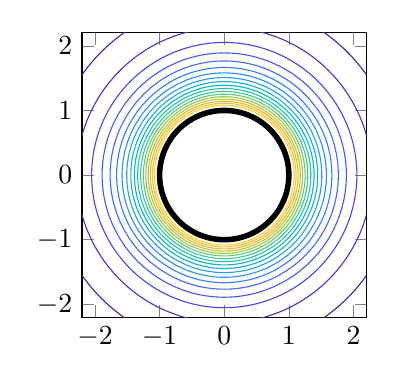
\begin{tikzpicture}

\begin{axis}[%
width=1.422in,
height=1.422in,
at={(0.406in,0.406in)},
scale only axis,
colormap={mymap}{[1pt] rgb(0pt)=(0.2422,0.1504,0.6603); rgb(1pt)=(0.25039,0.164995,0.707614); rgb(2pt)=(0.257771,0.181781,0.751138); rgb(3pt)=(0.264729,0.197757,0.795214); rgb(4pt)=(0.270648,0.214676,0.836371); rgb(5pt)=(0.275114,0.234238,0.870986); rgb(6pt)=(0.2783,0.255871,0.899071); rgb(7pt)=(0.280333,0.278233,0.9221); rgb(8pt)=(0.281338,0.300595,0.941376); rgb(9pt)=(0.281014,0.322757,0.957886); rgb(10pt)=(0.279467,0.344671,0.971676); rgb(11pt)=(0.275971,0.366681,0.982905); rgb(12pt)=(0.269914,0.3892,0.9906); rgb(13pt)=(0.260243,0.412329,0.995157); rgb(14pt)=(0.244033,0.435833,0.998833); rgb(15pt)=(0.220643,0.460257,0.997286); rgb(16pt)=(0.196333,0.484719,0.989152); rgb(17pt)=(0.183405,0.507371,0.979795); rgb(18pt)=(0.178643,0.528857,0.968157); rgb(19pt)=(0.176438,0.549905,0.952019); rgb(20pt)=(0.168743,0.570262,0.935871); rgb(21pt)=(0.154,0.5902,0.9218); rgb(22pt)=(0.146029,0.609119,0.907857); rgb(23pt)=(0.138024,0.627629,0.89729); rgb(24pt)=(0.124814,0.645929,0.888343); rgb(25pt)=(0.111252,0.6635,0.876314); rgb(26pt)=(0.0952095,0.679829,0.859781); rgb(27pt)=(0.0688714,0.694771,0.839357); rgb(28pt)=(0.0296667,0.708167,0.816333); rgb(29pt)=(0.00357143,0.720267,0.7917); rgb(30pt)=(0.00665714,0.731214,0.766014); rgb(31pt)=(0.0433286,0.741095,0.73941); rgb(32pt)=(0.0963952,0.75,0.712038); rgb(33pt)=(0.140771,0.7584,0.684157); rgb(34pt)=(0.1717,0.766962,0.655443); rgb(35pt)=(0.193767,0.775767,0.6251); rgb(36pt)=(0.216086,0.7843,0.5923); rgb(37pt)=(0.246957,0.791795,0.556743); rgb(38pt)=(0.290614,0.79729,0.518829); rgb(39pt)=(0.340643,0.8008,0.478857); rgb(40pt)=(0.3909,0.802871,0.435448); rgb(41pt)=(0.445629,0.802419,0.390919); rgb(42pt)=(0.5044,0.7993,0.348); rgb(43pt)=(0.561562,0.794233,0.304481); rgb(44pt)=(0.617395,0.787619,0.261238); rgb(45pt)=(0.671986,0.779271,0.2227); rgb(46pt)=(0.7242,0.769843,0.191029); rgb(47pt)=(0.773833,0.759805,0.16461); rgb(48pt)=(0.820314,0.749814,0.153529); rgb(49pt)=(0.863433,0.7406,0.159633); rgb(50pt)=(0.903543,0.733029,0.177414); rgb(51pt)=(0.939257,0.728786,0.209957); rgb(52pt)=(0.972757,0.729771,0.239443); rgb(53pt)=(0.995648,0.743371,0.237148); rgb(54pt)=(0.996986,0.765857,0.219943); rgb(55pt)=(0.995205,0.789252,0.202762); rgb(56pt)=(0.9892,0.813567,0.188533); rgb(57pt)=(0.978629,0.838629,0.176557); rgb(58pt)=(0.967648,0.8639,0.16429); rgb(59pt)=(0.96101,0.889019,0.153676); rgb(60pt)=(0.959671,0.913457,0.142257); rgb(61pt)=(0.962795,0.937338,0.12651); rgb(62pt)=(0.969114,0.960629,0.106362); rgb(63pt)=(0.9769,0.9839,0.0805)},
xmin=-2.2000,
xmax=2.2000,
ymin=-2.2000,
ymax=2.2000,
axis background/.style={fill=white}
]
\addplot[contour prepared, contour prepared format=matlab, contour/labels=false] table[row sep=crcr] {%
%
0.0476	59.0000\\
0.9997	-2.5000\\
1.0176	-2.4930\\
1.0678	-2.4722\\
1.1173	-2.4497\\
1.1181	-2.4494\\
1.1683	-2.4263\\
1.2186	-2.4010\\
1.2215	-2.3995\\
1.2688	-2.3752\\
1.3155	-2.3492\\
1.3191	-2.3473\\
1.3693	-2.3187\\
1.4016	-2.2990\\
1.4196	-2.2881\\
1.4698	-2.2561\\
1.4809	-2.2487\\
1.5201	-2.2228\\
1.5546	-2.1985\\
1.5704	-2.1874\\
1.6206	-2.1502\\
1.6232	-2.1482\\
1.6709	-2.1116\\
1.6878	-2.0980\\
1.7211	-2.0709\\
1.7485	-2.0477\\
1.7714	-2.0281\\
1.8057	-1.9975\\
1.8216	-1.9830\\
1.8597	-1.9472\\
1.8719	-1.9356\\
1.9110	-1.8970\\
1.9221	-1.8857\\
1.9596	-1.8467\\
1.9724	-1.8331\\
2.0058	-1.7965\\
2.0226	-1.7775\\
2.0498	-1.7462\\
2.0729	-1.7186\\
2.0916	-1.6960\\
2.1231	-1.6560\\
2.1312	-1.6457\\
2.1690	-1.5955\\
2.1734	-1.5894\\
2.2053	-1.5452\\
2.2236	-1.5184\\
2.2397	-1.4950\\
2.2721	-1.4447\\
2.2739	-1.4419\\
2.3037	-1.3945\\
2.3241	-1.3595\\
2.3332	-1.3442\\
2.3615	-1.2940\\
2.3744	-1.2697\\
2.3884	-1.2437\\
2.4139	-1.1935\\
2.4246	-1.1708\\
2.4381	-1.1432\\
2.4611	-1.0930\\
2.4749	-1.0604\\
0.0476	60.0000\\
-2.5000	-0.9997\\
-2.4828	-1.0427\\
-2.4610	-1.0930\\
-2.4497	-1.1173\\
-2.4381	-1.1432\\
-2.4139	-1.1935\\
-2.3995	-1.2215\\
-2.3884	-1.2437\\
-2.3615	-1.2940\\
-2.3492	-1.3156\\
-2.3333	-1.3442\\
-2.3034	-1.3945\\
-2.2990	-1.4015\\
-2.2725	-1.4447\\
-2.2487	-1.4809\\
-2.2396	-1.4950\\
-2.2051	-1.5452\\
-2.1985	-1.5545\\
-2.1692	-1.5955\\
-2.1482	-1.6233\\
-2.1313	-1.6457\\
-2.0980	-1.6877\\
-2.0914	-1.6960\\
-2.0495	-1.7462\\
-2.0477	-1.7483\\
-2.0057	-1.7965\\
-1.9975	-1.8056\\
-1.9596	-1.8467\\
-1.9472	-1.8597\\
-1.9110	-1.8970\\
-1.8970	-1.9110\\
-1.8597	-1.9472\\
-1.8467	-1.9596\\
-1.8056	-1.9975\\
-1.7965	-2.0057\\
-1.7483	-2.0477\\
-1.7462	-2.0495\\
-1.6960	-2.0914\\
-1.6877	-2.0980\\
-1.6457	-2.1313\\
-1.6233	-2.1482\\
-1.5955	-2.1692\\
-1.5545	-2.1985\\
-1.5452	-2.2051\\
-1.4950	-2.2396\\
-1.4809	-2.2487\\
-1.4447	-2.2725\\
-1.4015	-2.2990\\
-1.3945	-2.3034\\
-1.3442	-2.3333\\
-1.3156	-2.3492\\
-1.2940	-2.3615\\
-1.2437	-2.3884\\
-1.2215	-2.3995\\
-1.1935	-2.4139\\
-1.1432	-2.4381\\
-1.1173	-2.4497\\
-1.0930	-2.4610\\
-1.0427	-2.4828\\
-0.9997	-2.5000\\
0.0476	58.0000\\
2.4749	1.0604\\
2.4718	1.0678\\
2.4498	1.1181\\
2.4258	1.1683\\
2.4246	1.1708\\
2.4014	1.2186\\
2.3748	1.2688\\
2.3744	1.2696\\
2.3477	1.3191\\
2.3241	1.3595\\
2.3185	1.3693\\
2.2882	1.4196\\
2.2739	1.4420\\
2.2563	1.4698\\
2.2236	1.5183\\
2.2224	1.5201\\
2.1874	1.5704\\
2.1734	1.5895\\
2.1505	1.6206\\
2.1231	1.6561\\
2.1116	1.6709\\
2.0729	1.7184\\
2.0706	1.7211\\
2.0279	1.7714\\
2.0226	1.7773\\
1.9830	1.8216\\
1.9724	1.8330\\
1.9356	1.8719\\
1.9221	1.8857\\
1.8857	1.9221\\
1.8719	1.9356\\
1.8330	1.9724\\
1.8216	1.9830\\
1.7773	2.0226\\
1.7714	2.0279\\
1.7211	2.0706\\
1.7184	2.0729\\
1.6709	2.1116\\
1.6561	2.1231\\
1.6206	2.1505\\
1.5895	2.1734\\
1.5704	2.1874\\
1.5201	2.2224\\
1.5183	2.2236\\
1.4698	2.2563\\
1.4420	2.2739\\
1.4196	2.2882\\
1.3693	2.3185\\
1.3595	2.3241\\
1.3191	2.3477\\
1.2696	2.3744\\
1.2688	2.3748\\
1.2186	2.4014\\
1.1708	2.4246\\
1.1683	2.4258\\
1.1181	2.4498\\
1.0678	2.4718\\
1.0604	2.4749\\
0.0476	59.0000\\
-1.0604	2.4749\\
-1.0930	2.4611\\
-1.1432	2.4381\\
-1.1708	2.4246\\
-1.1935	2.4139\\
-1.2437	2.3884\\
-1.2697	2.3744\\
-1.2940	2.3615\\
-1.3442	2.3332\\
-1.3595	2.3241\\
-1.3945	2.3037\\
-1.4419	2.2739\\
-1.4447	2.2721\\
-1.4950	2.2397\\
-1.5184	2.2236\\
-1.5452	2.2053\\
-1.5894	2.1734\\
-1.5955	2.1690\\
-1.6457	2.1312\\
-1.6560	2.1231\\
-1.6960	2.0916\\
-1.7186	2.0729\\
-1.7462	2.0498\\
-1.7775	2.0226\\
-1.7965	2.0058\\
-1.8331	1.9724\\
-1.8467	1.9596\\
-1.8857	1.9221\\
-1.8970	1.9110\\
-1.9356	1.8719\\
-1.9472	1.8597\\
-1.9830	1.8216\\
-1.9975	1.8057\\
-2.0281	1.7714\\
-2.0477	1.7485\\
-2.0709	1.7211\\
-2.0980	1.6878\\
-2.1116	1.6709\\
-2.1482	1.6232\\
-2.1502	1.6206\\
-2.1874	1.5704\\
-2.1985	1.5546\\
-2.2228	1.5201\\
-2.2487	1.4809\\
-2.2561	1.4698\\
-2.2881	1.4196\\
-2.2990	1.4016\\
-2.3187	1.3693\\
-2.3473	1.3191\\
-2.3492	1.3155\\
-2.3752	1.2688\\
-2.3995	1.2215\\
-2.4010	1.2186\\
-2.4263	1.1683\\
-2.4494	1.1181\\
-2.4497	1.1173\\
-2.4722	1.0678\\
-2.4930	1.0176\\
-2.5000	0.9997\\
0.0476	161.0000\\
0.1155	-0.9925\\
0.1131	-0.9951\\
0.0628	-0.9951\\
0.0126	-0.9951\\
-0.0377	-0.9951\\
-0.0879	-0.9951\\
-0.0903	-0.9925\\
-0.1382	-0.9446\\
-0.1884	-0.9447\\
-0.2387	-0.9447\\
-0.2889	-0.9448\\
-0.2913	-0.9422\\
-0.3392	-0.8944\\
-0.3894	-0.8944\\
-0.4397	-0.8945\\
-0.4422	-0.8920\\
-0.4899	-0.8442\\
-0.4923	-0.8417\\
-0.5402	-0.7939\\
-0.5905	-0.7940\\
-0.5929	-0.7915\\
-0.6407	-0.7437\\
-0.6432	-0.7412\\
-0.6910	-0.6934\\
-0.6934	-0.6910\\
-0.7412	-0.6432\\
-0.7437	-0.6407\\
-0.7915	-0.5929\\
-0.7940	-0.5905\\
-0.7939	-0.5402\\
-0.8417	-0.4923\\
-0.8442	-0.4899\\
-0.8920	-0.4422\\
-0.8945	-0.4397\\
-0.8944	-0.3894\\
-0.8944	-0.3392\\
-0.9422	-0.2913\\
-0.9448	-0.2889\\
-0.9447	-0.2387\\
-0.9447	-0.1884\\
-0.9446	-0.1382\\
-0.9925	-0.0903\\
-0.9951	-0.0879\\
-0.9951	-0.0377\\
-0.9951	0.0126\\
-0.9951	0.0628\\
-0.9951	0.1131\\
-0.9925	0.1155\\
-0.9446	0.1633\\
-0.9447	0.2136\\
-0.9447	0.2638\\
-0.9448	0.3141\\
-0.9422	0.3165\\
-0.8944	0.3643\\
-0.8945	0.4146\\
-0.8920	0.4170\\
-0.8441	0.4648\\
-0.8442	0.5151\\
-0.8417	0.5175\\
-0.7939	0.5653\\
-0.7915	0.5677\\
-0.7436	0.6156\\
-0.7438	0.6658\\
-0.7412	0.6684\\
-0.6935	0.7161\\
-0.6910	0.7186\\
-0.6432	0.7663\\
-0.6407	0.7689\\
-0.5905	0.7688\\
-0.5426	0.8166\\
-0.5402	0.8191\\
-0.4924	0.8668\\
-0.4899	0.8694\\
-0.4397	0.8693\\
-0.3919	0.9171\\
-0.3894	0.9197\\
-0.3392	0.9196\\
-0.2889	0.9195\\
-0.2411	0.9673\\
-0.2387	0.9699\\
-0.1884	0.9699\\
-0.1382	0.9699\\
-0.0879	0.9698\\
-0.0377	0.9698\\
0.0126	0.9698\\
0.0628	0.9698\\
0.1131	0.9698\\
0.1633	0.9699\\
0.2136	0.9699\\
0.2160	0.9673\\
0.2638	0.9195\\
0.3141	0.9196\\
0.3643	0.9196\\
0.3667	0.9171\\
0.4146	0.8693\\
0.4648	0.8694\\
0.4673	0.8668\\
0.5151	0.8190\\
0.5653	0.8191\\
0.5678	0.8166\\
0.6156	0.7688\\
0.6180	0.7663\\
0.6658	0.7185\\
0.6683	0.7161\\
0.7161	0.6683\\
0.7185	0.6658\\
0.7663	0.6180\\
0.7688	0.6156\\
0.8166	0.5678\\
0.8191	0.5653\\
0.8190	0.5151\\
0.8668	0.4673\\
0.8694	0.4648\\
0.8693	0.4146\\
0.9171	0.3667\\
0.9196	0.3643\\
0.9196	0.3141\\
0.9195	0.2638\\
0.9673	0.2160\\
0.9699	0.2136\\
0.9699	0.1633\\
0.9698	0.1131\\
0.9698	0.0628\\
0.9698	0.0126\\
0.9698	-0.0377\\
0.9698	-0.0879\\
0.9699	-0.1382\\
0.9699	-0.1884\\
0.9699	-0.2387\\
0.9673	-0.2411\\
0.9195	-0.2889\\
0.9196	-0.3392\\
0.9197	-0.3894\\
0.9171	-0.3919\\
0.8693	-0.4397\\
0.8694	-0.4899\\
0.8668	-0.4924\\
0.8191	-0.5402\\
0.8166	-0.5426\\
0.7688	-0.5905\\
0.7689	-0.6407\\
0.7663	-0.6432\\
0.7186	-0.6910\\
0.7161	-0.6935\\
0.6684	-0.7412\\
0.6658	-0.7438\\
0.6156	-0.7436\\
0.5677	-0.7915\\
0.5653	-0.7939\\
0.5175	-0.8417\\
0.5151	-0.8442\\
0.4648	-0.8441\\
0.4170	-0.8920\\
0.4146	-0.8945\\
0.3643	-0.8944\\
0.3165	-0.9422\\
0.3141	-0.9448\\
0.2638	-0.9447\\
0.2136	-0.9447\\
0.1633	-0.9446\\
0.1155	-0.9925\\
0.0952	365.0000\\
-0.4024	-2.2487\\
-0.3894	-2.2512\\
-0.3392	-2.2596\\
-0.2889	-2.2667\\
-0.2387	-2.2726\\
-0.1884	-2.2773\\
-0.1382	-2.2809\\
-0.0879	-2.2834\\
-0.0377	-2.2847\\
0.0126	-2.2850\\
0.0628	-2.2842\\
0.1131	-2.2823\\
0.1633	-2.2792\\
0.2136	-2.2751\\
0.2638	-2.2698\\
0.3141	-2.2633\\
0.3643	-2.2556\\
0.4024	-2.2487\\
0.4146	-2.2467\\
0.4648	-2.2372\\
0.5151	-2.2263\\
0.5653	-2.2140\\
0.6156	-2.2001\\
0.6210	-2.1985\\
0.6658	-2.1858\\
0.7161	-2.1699\\
0.7663	-2.1523\\
0.7772	-2.1482\\
0.8166	-2.1340\\
0.8668	-2.1141\\
0.9042	-2.0980\\
0.9171	-2.0926\\
0.9673	-2.0701\\
1.0129	-2.0477\\
1.0176	-2.0455\\
1.0678	-2.0201\\
1.1087	-1.9975\\
1.1181	-1.9924\\
1.1683	-1.9636\\
1.1949	-1.9472\\
1.2186	-1.9328\\
1.2688	-1.8999\\
1.2731	-1.8970\\
1.3191	-1.8656\\
1.3451	-1.8467\\
1.3693	-1.8290\\
1.4114	-1.7965\\
1.4196	-1.7901\\
1.4698	-1.7490\\
1.4731	-1.7462\\
1.5201	-1.7056\\
1.5308	-1.6960\\
1.5704	-1.6595\\
1.5848	-1.6457\\
1.6206	-1.6105\\
1.6354	-1.5955\\
1.6709	-1.5582\\
1.6829	-1.5452\\
1.7211	-1.5024\\
1.7276	-1.4950\\
1.7698	-1.4447\\
1.7714	-1.4428\\
1.8099	-1.3945\\
1.8216	-1.3789\\
1.8476	-1.3442\\
1.8719	-1.3098\\
1.8831	-1.2940\\
1.9165	-1.2437\\
1.9221	-1.2348\\
1.9485	-1.1935\\
1.9724	-1.1529\\
1.9781	-1.1432\\
2.0065	-1.0930\\
2.0226	-1.0622\\
2.0330	-1.0427\\
2.0581	-0.9925\\
2.0729	-0.9604\\
2.0815	-0.9422\\
2.1037	-0.8920\\
2.1231	-0.8435\\
2.1239	-0.8417\\
2.1436	-0.7915\\
2.1614	-0.7412\\
2.1734	-0.7039\\
2.1777	-0.6910\\
2.1934	-0.6407\\
2.2074	-0.5905\\
2.2199	-0.5402\\
2.2236	-0.5237\\
2.2317	-0.4899\\
2.2424	-0.4397\\
2.2517	-0.3894\\
2.2597	-0.3392\\
2.2665	-0.2889\\
2.2721	-0.2387\\
2.2739	-0.2194\\
2.2769	-0.1884\\
2.2806	-0.1382\\
2.2832	-0.0879\\
2.2846	-0.0377\\
2.2849	0.0126\\
2.2840	0.0628\\
2.2821	0.1131\\
2.2789	0.1633\\
2.2746	0.2136\\
2.2739	0.2200\\
2.2695	0.2638\\
2.2632	0.3141\\
2.2558	0.3643\\
2.2472	0.4146\\
2.2372	0.4648\\
2.2258	0.5151\\
2.2236	0.5239\\
2.2138	0.5653\\
2.2006	0.6156\\
2.1858	0.6658\\
2.1734	0.7038\\
2.1696	0.7161\\
2.1527	0.7663\\
2.1340	0.8166\\
2.1231	0.8434\\
2.1140	0.8668\\
2.0929	0.9171\\
2.0729	0.9604\\
2.0698	0.9673\\
2.0459	1.0176\\
2.0226	1.0622\\
2.0197	1.0678\\
1.9927	1.1181\\
1.9724	1.1529\\
1.9635	1.1683\\
1.9327	1.2186\\
1.9221	1.2349\\
1.9002	1.2688\\
1.8719	1.3098\\
1.8654	1.3191\\
1.8289	1.3693\\
1.8216	1.3789\\
1.7903	1.4196\\
1.7714	1.4430\\
1.7493	1.4698\\
1.7211	1.5026\\
1.7057	1.5201\\
1.6709	1.5582\\
1.6595	1.5704\\
1.6206	1.6104\\
1.6104	1.6206\\
1.5704	1.6595\\
1.5582	1.6709\\
1.5201	1.7057\\
1.5026	1.7211\\
1.4698	1.7493\\
1.4430	1.7714\\
1.4196	1.7903\\
1.3789	1.8216\\
1.3693	1.8289\\
1.3191	1.8654\\
1.3098	1.8719\\
1.2688	1.9002\\
1.2349	1.9221\\
1.2186	1.9327\\
1.1683	1.9635\\
1.1529	1.9724\\
1.1181	1.9927\\
1.0678	2.0197\\
1.0622	2.0226\\
1.0176	2.0459\\
0.9673	2.0698\\
0.9604	2.0729\\
0.9171	2.0929\\
0.8668	2.1140\\
0.8434	2.1231\\
0.8166	2.1340\\
0.7663	2.1527\\
0.7161	2.1696\\
0.7038	2.1734\\
0.6658	2.1858\\
0.6156	2.2006\\
0.5653	2.2138\\
0.5239	2.2236\\
0.5151	2.2258\\
0.4648	2.2372\\
0.4146	2.2472\\
0.3643	2.2558\\
0.3141	2.2632\\
0.2638	2.2695\\
0.2200	2.2739\\
0.2136	2.2746\\
0.1633	2.2789\\
0.1131	2.2821\\
0.0628	2.2840\\
0.0126	2.2849\\
-0.0377	2.2846\\
-0.0879	2.2832\\
-0.1382	2.2806\\
-0.1884	2.2769\\
-0.2194	2.2739\\
-0.2387	2.2721\\
-0.2889	2.2665\\
-0.3392	2.2597\\
-0.3894	2.2517\\
-0.4397	2.2424\\
-0.4899	2.2317\\
-0.5237	2.2236\\
-0.5402	2.2199\\
-0.5905	2.2074\\
-0.6407	2.1934\\
-0.6910	2.1777\\
-0.7039	2.1734\\
-0.7412	2.1614\\
-0.7915	2.1436\\
-0.8417	2.1239\\
-0.8435	2.1231\\
-0.8920	2.1037\\
-0.9422	2.0815\\
-0.9604	2.0729\\
-0.9925	2.0581\\
-1.0427	2.0330\\
-1.0622	2.0226\\
-1.0930	2.0065\\
-1.1432	1.9781\\
-1.1529	1.9724\\
-1.1935	1.9485\\
-1.2348	1.9221\\
-1.2437	1.9165\\
-1.2940	1.8831\\
-1.3098	1.8719\\
-1.3442	1.8476\\
-1.3789	1.8216\\
-1.3945	1.8099\\
-1.4428	1.7714\\
-1.4447	1.7698\\
-1.4950	1.7276\\
-1.5024	1.7211\\
-1.5452	1.6829\\
-1.5582	1.6709\\
-1.5955	1.6354\\
-1.6105	1.6206\\
-1.6457	1.5848\\
-1.6595	1.5704\\
-1.6960	1.5308\\
-1.7056	1.5201\\
-1.7462	1.4731\\
-1.7490	1.4698\\
-1.7901	1.4196\\
-1.7965	1.4114\\
-1.8290	1.3693\\
-1.8467	1.3451\\
-1.8656	1.3191\\
-1.8970	1.2731\\
-1.8999	1.2688\\
-1.9328	1.2186\\
-1.9472	1.1949\\
-1.9636	1.1683\\
-1.9924	1.1181\\
-1.9975	1.1087\\
-2.0201	1.0678\\
-2.0455	1.0176\\
-2.0477	1.0129\\
-2.0701	0.9673\\
-2.0926	0.9171\\
-2.0980	0.9042\\
-2.1141	0.8668\\
-2.1340	0.8166\\
-2.1482	0.7772\\
-2.1523	0.7663\\
-2.1699	0.7161\\
-2.1858	0.6658\\
-2.1985	0.6210\\
-2.2001	0.6156\\
-2.2140	0.5653\\
-2.2263	0.5151\\
-2.2372	0.4648\\
-2.2467	0.4146\\
-2.2487	0.4024\\
-2.2556	0.3643\\
-2.2633	0.3141\\
-2.2698	0.2638\\
-2.2751	0.2136\\
-2.2792	0.1633\\
-2.2823	0.1131\\
-2.2842	0.0628\\
-2.2850	0.0126\\
-2.2847	-0.0377\\
-2.2834	-0.0879\\
-2.2809	-0.1382\\
-2.2773	-0.1884\\
-2.2726	-0.2387\\
-2.2667	-0.2889\\
-2.2596	-0.3392\\
-2.2512	-0.3894\\
-2.2487	-0.4024\\
-2.2421	-0.4397\\
-2.2319	-0.4899\\
-2.2203	-0.5402\\
-2.2072	-0.5905\\
-2.1985	-0.6208\\
-2.1931	-0.6407\\
-2.1781	-0.6910\\
-2.1614	-0.7412\\
-2.1482	-0.7772\\
-2.1433	-0.7915\\
-2.1243	-0.8417\\
-2.1034	-0.8920\\
-2.0980	-0.9042\\
-2.0816	-0.9422\\
-2.0580	-0.9925\\
-2.0477	-1.0129\\
-2.0331	-1.0427\\
-2.0064	-1.0930\\
-1.9975	-1.1088\\
-1.9784	-1.1432\\
-1.9481	-1.1935\\
-1.9472	-1.1948\\
-1.9167	-1.2437\\
-1.8970	-1.2732\\
-1.8831	-1.2940\\
-1.8472	-1.3442\\
-1.8467	-1.3449\\
-1.8099	-1.3945\\
-1.7965	-1.4115\\
-1.7701	-1.4447\\
-1.7462	-1.4733\\
-1.7278	-1.4950\\
-1.6960	-1.5308\\
-1.6829	-1.5452\\
-1.6457	-1.5847\\
-1.6353	-1.5955\\
-1.5955	-1.6353\\
-1.5847	-1.6457\\
-1.5452	-1.6829\\
-1.5308	-1.6960\\
-1.4950	-1.7278\\
-1.4733	-1.7462\\
-1.4447	-1.7701\\
-1.4115	-1.7965\\
-1.3945	-1.8099\\
-1.3449	-1.8467\\
-1.3442	-1.8472\\
-1.2940	-1.8831\\
-1.2732	-1.8970\\
-1.2437	-1.9167\\
-1.1948	-1.9472\\
-1.1935	-1.9481\\
-1.1432	-1.9784\\
-1.1088	-1.9975\\
-1.0930	-2.0064\\
-1.0427	-2.0331\\
-1.0129	-2.0477\\
-0.9925	-2.0580\\
-0.9422	-2.0816\\
-0.9042	-2.0980\\
-0.8920	-2.1034\\
-0.8417	-2.1243\\
-0.7915	-2.1433\\
-0.7772	-2.1482\\
-0.7412	-2.1614\\
-0.6910	-2.1781\\
-0.6407	-2.1931\\
-0.6208	-2.1985\\
-0.5905	-2.2072\\
-0.5402	-2.2203\\
-0.4899	-2.2319\\
-0.4397	-2.2421\\
-0.4024	-2.2487\\
0.0952	161.0000\\
0.1179	-0.9925\\
0.1131	-0.9977\\
0.0628	-0.9977\\
0.0126	-0.9977\\
-0.0377	-0.9977\\
-0.0879	-0.9977\\
-0.0927	-0.9925\\
-0.1382	-0.9470\\
-0.1884	-0.9471\\
-0.2387	-0.9472\\
-0.2889	-0.9473\\
-0.2937	-0.9422\\
-0.3392	-0.8968\\
-0.3894	-0.8969\\
-0.4397	-0.8971\\
-0.4446	-0.8920\\
-0.4899	-0.8467\\
-0.4947	-0.8417\\
-0.5402	-0.7962\\
-0.5905	-0.7965\\
-0.5954	-0.7915\\
-0.6407	-0.7462\\
-0.6456	-0.7412\\
-0.6910	-0.6959\\
-0.6959	-0.6910\\
-0.7412	-0.6456\\
-0.7462	-0.6407\\
-0.7915	-0.5954\\
-0.7965	-0.5905\\
-0.7962	-0.5402\\
-0.8417	-0.4947\\
-0.8467	-0.4899\\
-0.8920	-0.4446\\
-0.8971	-0.4397\\
-0.8969	-0.3894\\
-0.8968	-0.3392\\
-0.9422	-0.2937\\
-0.9473	-0.2889\\
-0.9472	-0.2387\\
-0.9471	-0.1884\\
-0.9470	-0.1382\\
-0.9925	-0.0927\\
-0.9977	-0.0879\\
-0.9977	-0.0377\\
-0.9977	0.0126\\
-0.9977	0.0628\\
-0.9977	0.1131\\
-0.9925	0.1179\\
-0.9470	0.1633\\
-0.9471	0.2136\\
-0.9472	0.2638\\
-0.9474	0.3141\\
-0.9422	0.3189\\
-0.8968	0.3643\\
-0.8970	0.4146\\
-0.8920	0.4194\\
-0.8465	0.4648\\
-0.8468	0.5151\\
-0.8417	0.5200\\
-0.7964	0.5653\\
-0.7915	0.5701\\
-0.7460	0.6156\\
-0.7463	0.6658\\
-0.7412	0.6709\\
-0.6960	0.7161\\
-0.6910	0.7212\\
-0.6458	0.7663\\
-0.6407	0.7715\\
-0.5905	0.7712\\
-0.5451	0.8166\\
-0.5402	0.8216\\
-0.4949	0.8668\\
-0.4899	0.8720\\
-0.4397	0.8718\\
-0.3944	0.9171\\
-0.3894	0.9223\\
-0.3392	0.9221\\
-0.2889	0.9220\\
-0.2436	0.9673\\
-0.2387	0.9726\\
-0.1884	0.9725\\
-0.1382	0.9724\\
-0.0879	0.9723\\
-0.0377	0.9723\\
0.0126	0.9723\\
0.0628	0.9723\\
0.1131	0.9723\\
0.1633	0.9724\\
0.2136	0.9725\\
0.2184	0.9673\\
0.2638	0.9219\\
0.3141	0.9220\\
0.3643	0.9222\\
0.3692	0.9171\\
0.4146	0.8717\\
0.4648	0.8719\\
0.4697	0.8668\\
0.5151	0.8214\\
0.5653	0.8217\\
0.5703	0.8166\\
0.6156	0.7713\\
0.6205	0.7663\\
0.6658	0.7210\\
0.6707	0.7161\\
0.7161	0.6707\\
0.7210	0.6658\\
0.7663	0.6205\\
0.7713	0.6156\\
0.8166	0.5703\\
0.8217	0.5653\\
0.8214	0.5151\\
0.8668	0.4697\\
0.8719	0.4648\\
0.8717	0.4146\\
0.9171	0.3692\\
0.9222	0.3643\\
0.9220	0.3141\\
0.9219	0.2638\\
0.9673	0.2184\\
0.9725	0.2136\\
0.9724	0.1633\\
0.9723	0.1131\\
0.9723	0.0628\\
0.9723	0.0126\\
0.9723	-0.0377\\
0.9723	-0.0879\\
0.9724	-0.1382\\
0.9725	-0.1884\\
0.9726	-0.2387\\
0.9673	-0.2436\\
0.9220	-0.2889\\
0.9221	-0.3392\\
0.9223	-0.3894\\
0.9171	-0.3944\\
0.8718	-0.4397\\
0.8720	-0.4899\\
0.8668	-0.4949\\
0.8216	-0.5402\\
0.8166	-0.5451\\
0.7712	-0.5905\\
0.7715	-0.6407\\
0.7663	-0.6458\\
0.7212	-0.6910\\
0.7161	-0.6960\\
0.6709	-0.7412\\
0.6658	-0.7463\\
0.6156	-0.7460\\
0.5701	-0.7915\\
0.5653	-0.7964\\
0.5200	-0.8417\\
0.5151	-0.8468\\
0.4648	-0.8465\\
0.4194	-0.8920\\
0.4146	-0.8970\\
0.3643	-0.8968\\
0.3189	-0.9422\\
0.3141	-0.9474\\
0.2638	-0.9472\\
0.2136	-0.9471\\
0.1633	-0.9470\\
0.1179	-0.9925\\
0.1429	329.0000\\
-0.1252	-2.0477\\
-0.0879	-2.0499\\
-0.0377	-2.0515\\
0.0126	-2.0518\\
0.0628	-2.0508\\
0.1131	-2.0486\\
0.1253	-2.0477\\
0.1633	-2.0453\\
0.2136	-2.0408\\
0.2638	-2.0351\\
0.3141	-2.0280\\
0.3643	-2.0196\\
0.4146	-2.0098\\
0.4648	-1.9984\\
0.4683	-1.9975\\
0.5151	-1.9864\\
0.5653	-1.9728\\
0.6156	-1.9575\\
0.6460	-1.9472\\
0.6658	-1.9409\\
0.7161	-1.9232\\
0.7663	-1.9034\\
0.7815	-1.8970\\
0.8166	-1.8826\\
0.8668	-1.8599\\
0.8938	-1.8467\\
0.9171	-1.8356\\
0.9673	-1.8097\\
0.9910	-1.7965\\
1.0176	-1.7819\\
1.0678	-1.7521\\
1.0771	-1.7462\\
1.1181	-1.7207\\
1.1547	-1.6960\\
1.1683	-1.6868\\
1.2186	-1.6507\\
1.2252	-1.6457\\
1.2688	-1.6126\\
1.2901	-1.5955\\
1.3191	-1.5718\\
1.3499	-1.5452\\
1.3693	-1.5281\\
1.4054	-1.4950\\
1.4196	-1.4815\\
1.4570	-1.4447\\
1.4698	-1.4316\\
1.5052	-1.3945\\
1.5201	-1.3782\\
1.5503	-1.3442\\
1.5704	-1.3206\\
1.5925	-1.2940\\
1.6206	-1.2584\\
1.6320	-1.2437\\
1.6689	-1.1935\\
1.6709	-1.1907\\
1.7040	-1.1432\\
1.7211	-1.1169\\
1.7367	-1.0930\\
1.7671	-1.0427\\
1.7714	-1.0353\\
1.7961	-0.9925\\
1.8216	-0.9440\\
1.8226	-0.9422\\
1.8481	-0.8920\\
1.8711	-0.8417\\
1.8719	-0.8399\\
1.8934	-0.7915\\
1.9134	-0.7412\\
1.9221	-0.7174\\
1.9322	-0.6910\\
1.9496	-0.6407\\
1.9652	-0.5905\\
1.9724	-0.5646\\
1.9795	-0.5402\\
1.9929	-0.4899\\
2.0045	-0.4397\\
2.0147	-0.3894\\
2.0226	-0.3439\\
2.0235	-0.3392\\
2.0316	-0.2889\\
2.0382	-0.2387\\
2.0436	-0.1884\\
2.0476	-0.1382\\
2.0504	-0.0879\\
2.0519	-0.0377\\
2.0522	0.0126\\
2.0513	0.0628\\
2.0491	0.1131\\
2.0457	0.1633\\
2.0411	0.2136\\
2.0351	0.2638\\
2.0277	0.3141\\
2.0226	0.3433\\
2.0192	0.3643\\
2.0098	0.4146\\
1.9989	0.4648\\
1.9864	0.5151\\
1.9724	0.5649\\
1.9723	0.5653\\
1.9576	0.6156\\
1.9411	0.6658\\
1.9227	0.7161\\
1.9221	0.7175\\
1.9037	0.7663\\
1.8825	0.8166\\
1.8719	0.8399\\
1.8599	0.8668\\
1.8357	0.9171\\
1.8216	0.9440\\
1.8097	0.9673\\
1.7818	1.0176\\
1.7714	1.0353\\
1.7523	1.0678\\
1.7211	1.1168\\
1.7203	1.1181\\
1.6869	1.1683\\
1.6709	1.1908\\
1.6510	1.2186\\
1.6206	1.2583\\
1.6125	1.2688\\
1.5715	1.3191\\
1.5704	1.3204\\
1.5280	1.3693\\
1.5201	1.3781\\
1.4815	1.4196\\
1.4698	1.4316\\
1.4316	1.4698\\
1.4196	1.4815\\
1.3781	1.5201\\
1.3693	1.5280\\
1.3204	1.5704\\
1.3191	1.5715\\
1.2688	1.6125\\
1.2583	1.6206\\
1.2186	1.6510\\
1.1908	1.6709\\
1.1683	1.6869\\
1.1181	1.7203\\
1.1168	1.7211\\
1.0678	1.7523\\
1.0353	1.7714\\
1.0176	1.7818\\
0.9673	1.8097\\
0.9440	1.8216\\
0.9171	1.8357\\
0.8668	1.8599\\
0.8399	1.8719\\
0.8166	1.8825\\
0.7663	1.9037\\
0.7175	1.9221\\
0.7161	1.9227\\
0.6658	1.9411\\
0.6156	1.9576\\
0.5653	1.9723\\
0.5649	1.9724\\
0.5151	1.9864\\
0.4648	1.9989\\
0.4146	2.0098\\
0.3643	2.0192\\
0.3433	2.0226\\
0.3141	2.0277\\
0.2638	2.0351\\
0.2136	2.0411\\
0.1633	2.0457\\
0.1131	2.0491\\
0.0628	2.0513\\
0.0126	2.0522\\
-0.0377	2.0519\\
-0.0879	2.0504\\
-0.1382	2.0476\\
-0.1884	2.0436\\
-0.2387	2.0382\\
-0.2889	2.0316\\
-0.3392	2.0235\\
-0.3439	2.0226\\
-0.3894	2.0147\\
-0.4397	2.0045\\
-0.4899	1.9929\\
-0.5402	1.9795\\
-0.5646	1.9724\\
-0.5905	1.9652\\
-0.6407	1.9496\\
-0.6910	1.9322\\
-0.7174	1.9221\\
-0.7412	1.9134\\
-0.7915	1.8934\\
-0.8399	1.8719\\
-0.8417	1.8711\\
-0.8920	1.8481\\
-0.9422	1.8226\\
-0.9440	1.8216\\
-0.9925	1.7961\\
-1.0353	1.7714\\
-1.0427	1.7671\\
-1.0930	1.7367\\
-1.1169	1.7211\\
-1.1432	1.7040\\
-1.1907	1.6709\\
-1.1935	1.6689\\
-1.2437	1.6320\\
-1.2584	1.6206\\
-1.2940	1.5925\\
-1.3206	1.5704\\
-1.3442	1.5503\\
-1.3782	1.5201\\
-1.3945	1.5052\\
-1.4316	1.4698\\
-1.4447	1.4570\\
-1.4815	1.4196\\
-1.4950	1.4054\\
-1.5281	1.3693\\
-1.5452	1.3499\\
-1.5718	1.3191\\
-1.5955	1.2901\\
-1.6126	1.2688\\
-1.6457	1.2252\\
-1.6507	1.2186\\
-1.6868	1.1683\\
-1.6960	1.1547\\
-1.7207	1.1181\\
-1.7462	1.0771\\
-1.7521	1.0678\\
-1.7819	1.0176\\
-1.7965	0.9910\\
-1.8097	0.9673\\
-1.8356	0.9171\\
-1.8467	0.8938\\
-1.8599	0.8668\\
-1.8826	0.8166\\
-1.8970	0.7815\\
-1.9034	0.7663\\
-1.9232	0.7161\\
-1.9409	0.6658\\
-1.9472	0.6460\\
-1.9575	0.6156\\
-1.9728	0.5653\\
-1.9864	0.5151\\
-1.9975	0.4683\\
-1.9984	0.4648\\
-2.0098	0.4146\\
-2.0196	0.3643\\
-2.0280	0.3141\\
-2.0351	0.2638\\
-2.0408	0.2136\\
-2.0453	0.1633\\
-2.0477	0.1253\\
-2.0486	0.1131\\
-2.0508	0.0628\\
-2.0518	0.0126\\
-2.0515	-0.0377\\
-2.0499	-0.0879\\
-2.0477	-0.1252\\
-2.0471	-0.1382\\
-2.0432	-0.1884\\
-2.0381	-0.2387\\
-2.0317	-0.2889\\
-2.0240	-0.3392\\
-2.0149	-0.3894\\
-2.0043	-0.4397\\
-1.9975	-0.4679\\
-1.9925	-0.4899\\
-1.9798	-0.5402\\
-1.9654	-0.5905\\
-1.9491	-0.6407\\
-1.9472	-0.6462\\
-1.9323	-0.6910\\
-1.9136	-0.7412\\
-1.8970	-0.7815\\
-1.8930	-0.7915\\
-1.8716	-0.8417\\
-1.8477	-0.8920\\
-1.8467	-0.8938\\
-1.8230	-0.9422\\
-1.7965	-0.9910\\
-1.7957	-0.9925\\
-1.7674	-1.0427\\
-1.7462	-1.0771\\
-1.7366	-1.0930\\
-1.7039	-1.1432\\
-1.6960	-1.1547\\
-1.6692	-1.1935\\
-1.6457	-1.2253\\
-1.6320	-1.2437\\
-1.5955	-1.2900\\
-1.5923	-1.2940\\
-1.5501	-1.3442\\
-1.5452	-1.3498\\
-1.5051	-1.3945\\
-1.4950	-1.4053\\
-1.4570	-1.4447\\
-1.4447	-1.4570\\
-1.4053	-1.4950\\
-1.3945	-1.5051\\
-1.3498	-1.5452\\
-1.3442	-1.5501\\
-1.2940	-1.5923\\
-1.2900	-1.5955\\
-1.2437	-1.6320\\
-1.2253	-1.6457\\
-1.1935	-1.6692\\
-1.1547	-1.6960\\
-1.1432	-1.7039\\
-1.0930	-1.7366\\
-1.0771	-1.7462\\
-1.0427	-1.7674\\
-0.9925	-1.7957\\
-0.9910	-1.7965\\
-0.9422	-1.8230\\
-0.8938	-1.8467\\
-0.8920	-1.8477\\
-0.8417	-1.8716\\
-0.7915	-1.8930\\
-0.7815	-1.8970\\
-0.7412	-1.9136\\
-0.6910	-1.9323\\
-0.6462	-1.9472\\
-0.6407	-1.9491\\
-0.5905	-1.9654\\
-0.5402	-1.9798\\
-0.4899	-1.9925\\
-0.4679	-1.9975\\
-0.4397	-2.0043\\
-0.3894	-2.0149\\
-0.3392	-2.0240\\
-0.2889	-2.0317\\
-0.2387	-2.0381\\
-0.1884	-2.0432\\
-0.1382	-2.0471\\
-0.1252	-2.0477\\
0.1429	161.0000\\
0.1203	-0.9925\\
0.1131	-1.0003\\
0.0628	-1.0003\\
0.0126	-1.0002\\
-0.0377	-1.0003\\
-0.0879	-1.0003\\
-0.0951	-0.9925\\
-0.1382	-0.9494\\
-0.1884	-0.9495\\
-0.2387	-0.9497\\
-0.2889	-0.9499\\
-0.2961	-0.9422\\
-0.3392	-0.8992\\
-0.3894	-0.8994\\
-0.4397	-0.8997\\
-0.4471	-0.8920\\
-0.4899	-0.8491\\
-0.4971	-0.8417\\
-0.5402	-0.7986\\
-0.5905	-0.7990\\
-0.5979	-0.7915\\
-0.6407	-0.7486\\
-0.6481	-0.7412\\
-0.6910	-0.6983\\
-0.6983	-0.6910\\
-0.7412	-0.6481\\
-0.7486	-0.6407\\
-0.7915	-0.5979\\
-0.7990	-0.5905\\
-0.7986	-0.5402\\
-0.8417	-0.4971\\
-0.8491	-0.4899\\
-0.8920	-0.4471\\
-0.8997	-0.4397\\
-0.8994	-0.3894\\
-0.8992	-0.3392\\
-0.9422	-0.2961\\
-0.9499	-0.2889\\
-0.9497	-0.2387\\
-0.9495	-0.1884\\
-0.9494	-0.1382\\
-0.9925	-0.0951\\
-1.0003	-0.0879\\
-1.0003	-0.0377\\
-1.0002	0.0126\\
-1.0003	0.0628\\
-1.0003	0.1131\\
-0.9925	0.1203\\
-0.9495	0.1633\\
-0.9496	0.2136\\
-0.9498	0.2638\\
-0.9500	0.3141\\
-0.9422	0.3214\\
-0.8993	0.3643\\
-0.8995	0.4146\\
-0.8920	0.4218\\
-0.8490	0.4648\\
-0.8493	0.5151\\
-0.8417	0.5224\\
-0.7988	0.5653\\
-0.7915	0.5725\\
-0.7484	0.6156\\
-0.7489	0.6658\\
-0.7412	0.6734\\
-0.6986	0.7161\\
-0.6910	0.7237\\
-0.6483	0.7663\\
-0.6407	0.7740\\
-0.5905	0.7736\\
-0.5475	0.8166\\
-0.5402	0.8241\\
-0.4974	0.8668\\
-0.4899	0.8746\\
-0.4397	0.8742\\
-0.3969	0.9171\\
-0.3894	0.9249\\
-0.3392	0.9246\\
-0.2889	0.9244\\
-0.2460	0.9673\\
-0.2387	0.9752\\
-0.1884	0.9750\\
-0.1382	0.9749\\
-0.0879	0.9748\\
-0.0377	0.9748\\
0.0126	0.9748\\
0.0628	0.9748\\
0.1131	0.9748\\
0.1633	0.9749\\
0.2136	0.9751\\
0.2208	0.9673\\
0.2638	0.9243\\
0.3141	0.9245\\
0.3643	0.9247\\
0.3716	0.9171\\
0.4146	0.8741\\
0.4648	0.8744\\
0.4721	0.8668\\
0.5151	0.8239\\
0.5653	0.8243\\
0.5728	0.8166\\
0.6156	0.7738\\
0.6230	0.7663\\
0.6658	0.7235\\
0.6732	0.7161\\
0.7161	0.6732\\
0.7235	0.6658\\
0.7663	0.6230\\
0.7738	0.6156\\
0.8166	0.5728\\
0.8243	0.5653\\
0.8239	0.5151\\
0.8668	0.4721\\
0.8744	0.4648\\
0.8741	0.4146\\
0.9171	0.3716\\
0.9247	0.3643\\
0.9245	0.3141\\
0.9243	0.2638\\
0.9673	0.2208\\
0.9751	0.2136\\
0.9749	0.1633\\
0.9748	0.1131\\
0.9748	0.0628\\
0.9748	0.0126\\
0.9748	-0.0377\\
0.9748	-0.0879\\
0.9749	-0.1382\\
0.9750	-0.1884\\
0.9752	-0.2387\\
0.9673	-0.2460\\
0.9244	-0.2889\\
0.9246	-0.3392\\
0.9249	-0.3894\\
0.9171	-0.3969\\
0.8742	-0.4397\\
0.8746	-0.4899\\
0.8668	-0.4974\\
0.8241	-0.5402\\
0.8166	-0.5475\\
0.7736	-0.5905\\
0.7740	-0.6407\\
0.7663	-0.6483\\
0.7237	-0.6910\\
0.7161	-0.6986\\
0.6734	-0.7412\\
0.6658	-0.7489\\
0.6156	-0.7484\\
0.5725	-0.7915\\
0.5653	-0.7988\\
0.5224	-0.8417\\
0.5151	-0.8493\\
0.4648	-0.8490\\
0.4218	-0.8920\\
0.4146	-0.8995\\
0.3643	-0.8993\\
0.3214	-0.9422\\
0.3141	-0.9500\\
0.2638	-0.9498\\
0.2136	-0.9496\\
0.1633	-0.9495\\
0.1203	-0.9925\\
0.1905	301.0000\\
-0.3985	-1.8467\\
-0.3894	-1.8488\\
-0.3392	-1.8590\\
-0.2889	-1.8677\\
-0.2387	-1.8748\\
-0.1884	-1.8804\\
-0.1382	-1.8847\\
-0.0879	-1.8876\\
-0.0377	-1.8893\\
0.0126	-1.8896\\
0.0628	-1.8886\\
0.1131	-1.8863\\
0.1633	-1.8827\\
0.2136	-1.8778\\
0.2638	-1.8714\\
0.3141	-1.8635\\
0.3643	-1.8541\\
0.3983	-1.8467\\
0.4146	-1.8434\\
0.4648	-1.8317\\
0.5151	-1.8183\\
0.5653	-1.8030\\
0.5847	-1.7965\\
0.6156	-1.7866\\
0.6658	-1.7686\\
0.7161	-1.7484\\
0.7212	-1.7462\\
0.7663	-1.7274\\
0.8166	-1.7040\\
0.8325	-1.6960\\
0.8668	-1.6792\\
0.9171	-1.6520\\
0.9280	-1.6457\\
0.9673	-1.6233\\
1.0120	-1.5955\\
1.0176	-1.5920\\
1.0678	-1.5589\\
1.0872	-1.5452\\
1.1181	-1.5234\\
1.1554	-1.4950\\
1.1683	-1.4850\\
1.2175	-1.4447\\
1.2186	-1.4438\\
1.2688	-1.4000\\
1.2749	-1.3945\\
1.3191	-1.3528\\
1.3278	-1.3442\\
1.3693	-1.3018\\
1.3768	-1.2940\\
1.4196	-1.2468\\
1.4223	-1.2437\\
1.4648	-1.1935\\
1.4698	-1.1871\\
1.5045	-1.1432\\
1.5201	-1.1221\\
1.5415	-1.0930\\
1.5704	-1.0506\\
1.5757	-1.0427\\
1.6080	-0.9925\\
1.6206	-0.9712\\
1.6380	-0.9422\\
1.6657	-0.8920\\
1.6709	-0.8819\\
1.6919	-0.8417\\
1.7157	-0.7915\\
1.7211	-0.7792\\
1.7383	-0.7412\\
1.7588	-0.6910\\
1.7714	-0.6569\\
1.7776	-0.6407\\
1.7952	-0.5905\\
1.8108	-0.5402\\
1.8216	-0.5010\\
1.8248	-0.4899\\
1.8379	-0.4397\\
1.8493	-0.3894\\
1.8591	-0.3392\\
1.8673	-0.2889\\
1.8719	-0.2553\\
1.8743	-0.2387\\
1.8802	-0.1884\\
1.8847	-0.1382\\
1.8878	-0.0879\\
1.8895	-0.0377\\
1.8898	0.0126\\
1.8888	0.0628\\
1.8864	0.1131\\
1.8826	0.1633\\
1.8774	0.2136\\
1.8719	0.2556\\
1.8709	0.2638\\
1.8634	0.3141\\
1.8544	0.3643\\
1.8438	0.4146\\
1.8316	0.4648\\
1.8216	0.5009\\
1.8179	0.5151\\
1.8033	0.5653\\
1.7867	0.6156\\
1.7714	0.6570\\
1.7682	0.6658\\
1.7489	0.7161\\
1.7271	0.7663\\
1.7211	0.7792\\
1.7042	0.8166\\
1.6790	0.8668\\
1.6709	0.8819\\
1.6523	0.9171\\
1.6230	0.9673\\
1.6206	0.9712\\
1.5923	1.0176\\
1.5704	1.0506\\
1.5589	1.0678\\
1.5230	1.1181\\
1.5201	1.1220\\
1.4851	1.1683\\
1.4698	1.1872\\
1.4442	1.2186\\
1.4196	1.2469\\
1.4002	1.2688\\
1.3693	1.3019\\
1.3529	1.3191\\
1.3191	1.3529\\
1.3019	1.3693\\
1.2688	1.4002\\
1.2469	1.4196\\
1.2186	1.4442\\
1.1872	1.4698\\
1.1683	1.4851\\
1.1220	1.5201\\
1.1181	1.5230\\
1.0678	1.5589\\
1.0506	1.5704\\
1.0176	1.5923\\
0.9712	1.6206\\
0.9673	1.6230\\
0.9171	1.6523\\
0.8819	1.6709\\
0.8668	1.6790\\
0.8166	1.7042\\
0.7792	1.7211\\
0.7663	1.7271\\
0.7161	1.7489\\
0.6658	1.7682\\
0.6570	1.7714\\
0.6156	1.7867\\
0.5653	1.8033\\
0.5151	1.8179\\
0.5009	1.8216\\
0.4648	1.8316\\
0.4146	1.8438\\
0.3643	1.8544\\
0.3141	1.8634\\
0.2638	1.8709\\
0.2556	1.8719\\
0.2136	1.8774\\
0.1633	1.8826\\
0.1131	1.8864\\
0.0628	1.8888\\
0.0126	1.8898\\
-0.0377	1.8895\\
-0.0879	1.8878\\
-0.1382	1.8847\\
-0.1884	1.8802\\
-0.2387	1.8743\\
-0.2553	1.8719\\
-0.2889	1.8673\\
-0.3392	1.8591\\
-0.3894	1.8493\\
-0.4397	1.8379\\
-0.4899	1.8248\\
-0.5010	1.8216\\
-0.5402	1.8108\\
-0.5905	1.7952\\
-0.6407	1.7776\\
-0.6569	1.7714\\
-0.6910	1.7588\\
-0.7412	1.7383\\
-0.7792	1.7211\\
-0.7915	1.7157\\
-0.8417	1.6919\\
-0.8819	1.6709\\
-0.8920	1.6657\\
-0.9422	1.6380\\
-0.9712	1.6206\\
-0.9925	1.6080\\
-1.0427	1.5757\\
-1.0506	1.5704\\
-1.0930	1.5415\\
-1.1221	1.5201\\
-1.1432	1.5045\\
-1.1871	1.4698\\
-1.1935	1.4648\\
-1.2437	1.4223\\
-1.2468	1.4196\\
-1.2940	1.3768\\
-1.3018	1.3693\\
-1.3442	1.3278\\
-1.3528	1.3191\\
-1.3945	1.2749\\
-1.4000	1.2688\\
-1.4438	1.2186\\
-1.4447	1.2175\\
-1.4850	1.1683\\
-1.4950	1.1554\\
-1.5234	1.1181\\
-1.5452	1.0872\\
-1.5589	1.0678\\
-1.5920	1.0176\\
-1.5955	1.0120\\
-1.6233	0.9673\\
-1.6457	0.9280\\
-1.6520	0.9171\\
-1.6792	0.8668\\
-1.6960	0.8325\\
-1.7040	0.8166\\
-1.7274	0.7663\\
-1.7462	0.7212\\
-1.7484	0.7161\\
-1.7686	0.6658\\
-1.7866	0.6156\\
-1.7965	0.5847\\
-1.8030	0.5653\\
-1.8183	0.5151\\
-1.8317	0.4648\\
-1.8434	0.4146\\
-1.8467	0.3983\\
-1.8541	0.3643\\
-1.8635	0.3141\\
-1.8714	0.2638\\
-1.8778	0.2136\\
-1.8827	0.1633\\
-1.8863	0.1131\\
-1.8886	0.0628\\
-1.8896	0.0126\\
-1.8893	-0.0377\\
-1.8876	-0.0879\\
-1.8847	-0.1382\\
-1.8804	-0.1884\\
-1.8748	-0.2387\\
-1.8677	-0.2889\\
-1.8590	-0.3392\\
-1.8488	-0.3894\\
-1.8467	-0.3985\\
-1.8378	-0.4397\\
-1.8252	-0.4899\\
-1.8109	-0.5402\\
-1.7965	-0.5848\\
-1.7948	-0.5905\\
-1.7779	-0.6407\\
-1.7588	-0.6910\\
-1.7462	-0.7211\\
-1.7381	-0.7412\\
-1.7160	-0.7915\\
-1.6960	-0.8325\\
-1.6916	-0.8417\\
-1.6660	-0.8920\\
-1.6457	-0.9280\\
-1.6379	-0.9422\\
-1.6080	-0.9925\\
-1.5955	-1.0120\\
-1.5759	-1.0427\\
-1.5452	-1.0872\\
-1.5412	-1.0930\\
-1.5044	-1.1432\\
-1.4950	-1.1554\\
-1.4650	-1.1935\\
-1.4447	-1.2177\\
-1.4226	-1.2437\\
-1.3945	-1.2750\\
-1.3769	-1.2940\\
-1.3442	-1.3279\\
-1.3279	-1.3442\\
-1.2940	-1.3769\\
-1.2750	-1.3945\\
-1.2437	-1.4226\\
-1.2177	-1.4447\\
-1.1935	-1.4650\\
-1.1554	-1.4950\\
-1.1432	-1.5044\\
-1.0930	-1.5412\\
-1.0872	-1.5452\\
-1.0427	-1.5759\\
-1.0120	-1.5955\\
-0.9925	-1.6080\\
-0.9422	-1.6379\\
-0.9280	-1.6457\\
-0.8920	-1.6660\\
-0.8417	-1.6916\\
-0.8325	-1.6960\\
-0.7915	-1.7160\\
-0.7412	-1.7381\\
-0.7211	-1.7462\\
-0.6910	-1.7588\\
-0.6407	-1.7779\\
-0.5905	-1.7948\\
-0.5848	-1.7965\\
-0.5402	-1.8109\\
-0.4899	-1.8252\\
-0.4397	-1.8378\\
-0.3985	-1.8467\\
0.1905	161.0000\\
0.1227	-0.9925\\
0.1131	-1.0030\\
0.0628	-1.0029\\
0.0126	-1.0028\\
-0.0377	-1.0029\\
-0.0879	-1.0029\\
-0.0975	-0.9925\\
-0.1382	-0.9518\\
-0.1884	-0.9520\\
-0.2387	-0.9522\\
-0.2889	-0.9524\\
-0.2985	-0.9422\\
-0.3392	-0.9016\\
-0.3894	-0.9019\\
-0.4397	-0.9023\\
-0.4496	-0.8920\\
-0.4899	-0.8516\\
-0.4995	-0.8417\\
-0.5402	-0.8010\\
-0.5905	-0.8016\\
-0.6004	-0.7915\\
-0.6407	-0.7511\\
-0.6505	-0.7412\\
-0.6910	-0.7008\\
-0.7008	-0.6910\\
-0.7412	-0.6505\\
-0.7511	-0.6407\\
-0.7915	-0.6004\\
-0.8016	-0.5905\\
-0.8010	-0.5402\\
-0.8417	-0.4995\\
-0.8516	-0.4899\\
-0.8920	-0.4496\\
-0.9023	-0.4397\\
-0.9019	-0.3894\\
-0.9016	-0.3392\\
-0.9422	-0.2985\\
-0.9524	-0.2889\\
-0.9522	-0.2387\\
-0.9520	-0.1884\\
-0.9518	-0.1382\\
-0.9925	-0.0975\\
-1.0029	-0.0879\\
-1.0029	-0.0377\\
-1.0028	0.0126\\
-1.0029	0.0628\\
-1.0030	0.1131\\
-0.9925	0.1227\\
-0.9519	0.1633\\
-0.9521	0.2136\\
-0.9523	0.2638\\
-0.9526	0.3141\\
-0.9422	0.3238\\
-0.9017	0.3643\\
-0.9021	0.4146\\
-0.8920	0.4242\\
-0.8514	0.4648\\
-0.8518	0.5151\\
-0.8417	0.5249\\
-0.8013	0.5653\\
-0.7915	0.5749\\
-0.7508	0.6156\\
-0.7514	0.6658\\
-0.7412	0.6760\\
-0.7011	0.7161\\
-0.6910	0.7262\\
-0.6509	0.7663\\
-0.6407	0.7766\\
-0.5905	0.7760\\
-0.5499	0.8166\\
-0.5402	0.8265\\
-0.4999	0.8668\\
-0.4899	0.8772\\
-0.4397	0.8767\\
-0.3993	0.9171\\
-0.3894	0.9275\\
-0.3392	0.9271\\
-0.2889	0.9268\\
-0.2484	0.9673\\
-0.2387	0.9778\\
-0.1884	0.9776\\
-0.1382	0.9774\\
-0.0879	0.9773\\
-0.0377	0.9772\\
0.0126	0.9772\\
0.0628	0.9773\\
0.1131	0.9774\\
0.1633	0.9775\\
0.2136	0.9777\\
0.2232	0.9673\\
0.2638	0.9267\\
0.3141	0.9270\\
0.3643	0.9273\\
0.3740	0.9171\\
0.4146	0.8765\\
0.4648	0.8769\\
0.4745	0.8668\\
0.5151	0.8263\\
0.5653	0.8268\\
0.5753	0.8166\\
0.6156	0.7763\\
0.6254	0.7663\\
0.6658	0.7259\\
0.6756	0.7161\\
0.7161	0.6756\\
0.7259	0.6658\\
0.7663	0.6254\\
0.7763	0.6156\\
0.8166	0.5753\\
0.8268	0.5653\\
0.8263	0.5151\\
0.8668	0.4745\\
0.8769	0.4648\\
0.8765	0.4146\\
0.9171	0.3740\\
0.9273	0.3643\\
0.9270	0.3141\\
0.9267	0.2638\\
0.9673	0.2232\\
0.9777	0.2136\\
0.9775	0.1633\\
0.9774	0.1131\\
0.9773	0.0628\\
0.9772	0.0126\\
0.9772	-0.0377\\
0.9773	-0.0879\\
0.9774	-0.1382\\
0.9776	-0.1884\\
0.9778	-0.2387\\
0.9673	-0.2484\\
0.9268	-0.2889\\
0.9271	-0.3392\\
0.9275	-0.3894\\
0.9171	-0.3993\\
0.8767	-0.4397\\
0.8772	-0.4899\\
0.8668	-0.4999\\
0.8265	-0.5402\\
0.8166	-0.5499\\
0.7760	-0.5905\\
0.7766	-0.6407\\
0.7663	-0.6509\\
0.7262	-0.6910\\
0.7161	-0.7011\\
0.6760	-0.7412\\
0.6658	-0.7514\\
0.6156	-0.7508\\
0.5749	-0.7915\\
0.5653	-0.8013\\
0.5249	-0.8417\\
0.5151	-0.8518\\
0.4648	-0.8514\\
0.4242	-0.8920\\
0.4146	-0.9021\\
0.3643	-0.9017\\
0.3238	-0.9422\\
0.3141	-0.9526\\
0.2638	-0.9523\\
0.2136	-0.9521\\
0.1633	-0.9519\\
0.1227	-0.9925\\
0.2381	281.0000\\
-0.2565	-1.7462\\
-0.2387	-1.7490\\
-0.1884	-1.7554\\
-0.1382	-1.7602\\
-0.0879	-1.7635\\
-0.0377	-1.7653\\
0.0126	-1.7656\\
0.0628	-1.7646\\
0.1131	-1.7620\\
0.1633	-1.7580\\
0.2136	-1.7524\\
0.2570	-1.7462\\
0.2638	-1.7453\\
0.3141	-1.7373\\
0.3643	-1.7277\\
0.4146	-1.7163\\
0.4648	-1.7031\\
0.4888	-1.6960\\
0.5151	-1.6886\\
0.5653	-1.6727\\
0.6156	-1.6546\\
0.6379	-1.6457\\
0.6658	-1.6351\\
0.7161	-1.6138\\
0.7550	-1.5955\\
0.7663	-1.5903\\
0.8166	-1.5653\\
0.8532	-1.5452\\
0.8668	-1.5379\\
0.9171	-1.5085\\
0.9385	-1.4950\\
0.9673	-1.4769\\
1.0141	-1.4447\\
1.0176	-1.4424\\
1.0678	-1.4058\\
1.0823	-1.3945\\
1.1181	-1.3662\\
1.1442	-1.3442\\
1.1683	-1.3234\\
1.2008	-1.2940\\
1.2186	-1.2773\\
1.2528	-1.2437\\
1.2688	-1.2273\\
1.3008	-1.1935\\
1.3191	-1.1731\\
1.3452	-1.1432\\
1.3693	-1.1140\\
1.3864	-1.0930\\
1.4196	-1.0491\\
1.4244	-1.0427\\
1.4600	-0.9925\\
1.4698	-0.9774\\
1.4931	-0.9422\\
1.5201	-0.8972\\
1.5233	-0.8920\\
1.5520	-0.8417\\
1.5704	-0.8060\\
1.5780	-0.7915\\
1.6024	-0.7412\\
1.6206	-0.6994\\
1.6244	-0.6910\\
1.6453	-0.6407\\
1.6637	-0.5905\\
1.6709	-0.5688\\
1.6808	-0.5402\\
1.6963	-0.4899\\
1.7099	-0.4397\\
1.7211	-0.3916\\
1.7216	-0.3894\\
1.7326	-0.3392\\
1.7419	-0.2889\\
1.7495	-0.2387\\
1.7556	-0.1884\\
1.7601	-0.1382\\
1.7633	-0.0879\\
1.7650	-0.0377\\
1.7653	0.0126\\
1.7643	0.0628\\
1.7619	0.1131\\
1.7580	0.1633\\
1.7527	0.2136\\
1.7459	0.2638\\
1.7375	0.3141\\
1.7274	0.3643\\
1.7211	0.3911\\
1.7160	0.4146\\
1.7033	0.4648\\
1.6888	0.5151\\
1.6722	0.5653\\
1.6709	0.5690\\
1.6548	0.6156\\
1.6352	0.6658\\
1.6206	0.6994\\
1.6136	0.7161\\
1.5906	0.7663\\
1.5704	0.8060\\
1.5651	0.8166\\
1.5380	0.8668\\
1.5201	0.8972\\
1.5085	0.9171\\
1.4767	0.9673\\
1.4698	0.9774\\
1.4427	1.0176\\
1.4196	1.0491\\
1.4058	1.0678\\
1.3693	1.1139\\
1.3659	1.1181\\
1.3232	1.1683\\
1.3191	1.1730\\
1.2772	1.2186\\
1.2688	1.2272\\
1.2272	1.2688\\
1.2186	1.2772\\
1.1730	1.3191\\
1.1683	1.3232\\
1.1181	1.3659\\
1.1139	1.3693\\
1.0678	1.4058\\
1.0491	1.4196\\
1.0176	1.4427\\
0.9774	1.4698\\
0.9673	1.4767\\
0.9171	1.5085\\
0.8972	1.5201\\
0.8668	1.5380\\
0.8166	1.5651\\
0.8060	1.5704\\
0.7663	1.5906\\
0.7161	1.6136\\
0.6994	1.6206\\
0.6658	1.6352\\
0.6156	1.6548\\
0.5690	1.6709\\
0.5653	1.6722\\
0.5151	1.6888\\
0.4648	1.7033\\
0.4146	1.7160\\
0.3911	1.7211\\
0.3643	1.7274\\
0.3141	1.7375\\
0.2638	1.7459\\
0.2136	1.7527\\
0.1633	1.7580\\
0.1131	1.7619\\
0.0628	1.7643\\
0.0126	1.7653\\
-0.0377	1.7650\\
-0.0879	1.7633\\
-0.1382	1.7601\\
-0.1884	1.7556\\
-0.2387	1.7495\\
-0.2889	1.7419\\
-0.3392	1.7326\\
-0.3894	1.7216\\
-0.3916	1.7211\\
-0.4397	1.7099\\
-0.4899	1.6963\\
-0.5402	1.6808\\
-0.5688	1.6709\\
-0.5905	1.6637\\
-0.6407	1.6453\\
-0.6910	1.6244\\
-0.6994	1.6206\\
-0.7412	1.6024\\
-0.7915	1.5780\\
-0.8060	1.5704\\
-0.8417	1.5520\\
-0.8920	1.5233\\
-0.8972	1.5201\\
-0.9422	1.4931\\
-0.9774	1.4698\\
-0.9925	1.4600\\
-1.0427	1.4244\\
-1.0491	1.4196\\
-1.0930	1.3864\\
-1.1140	1.3693\\
-1.1432	1.3452\\
-1.1731	1.3191\\
-1.1935	1.3008\\
-1.2273	1.2688\\
-1.2437	1.2528\\
-1.2773	1.2186\\
-1.2940	1.2008\\
-1.3234	1.1683\\
-1.3442	1.1442\\
-1.3662	1.1181\\
-1.3945	1.0823\\
-1.4058	1.0678\\
-1.4424	1.0176\\
-1.4447	1.0141\\
-1.4769	0.9673\\
-1.4950	0.9385\\
-1.5085	0.9171\\
-1.5379	0.8668\\
-1.5452	0.8532\\
-1.5653	0.8166\\
-1.5903	0.7663\\
-1.5955	0.7550\\
-1.6138	0.7161\\
-1.6351	0.6658\\
-1.6457	0.6379\\
-1.6546	0.6156\\
-1.6727	0.5653\\
-1.6886	0.5151\\
-1.6960	0.4888\\
-1.7031	0.4648\\
-1.7163	0.4146\\
-1.7277	0.3643\\
-1.7373	0.3141\\
-1.7453	0.2638\\
-1.7462	0.2570\\
-1.7524	0.2136\\
-1.7580	0.1633\\
-1.7620	0.1131\\
-1.7646	0.0628\\
-1.7656	0.0126\\
-1.7653	-0.0377\\
-1.7635	-0.0879\\
-1.7602	-0.1382\\
-1.7554	-0.1884\\
-1.7490	-0.2387\\
-1.7462	-0.2565\\
-1.7415	-0.2889\\
-1.7327	-0.3392\\
-1.7222	-0.3894\\
-1.7099	-0.4397\\
-1.6960	-0.4892\\
-1.6958	-0.4899\\
-1.6809	-0.5402\\
-1.6639	-0.5905\\
-1.6457	-0.6381\\
-1.6448	-0.6407\\
-1.6248	-0.6910\\
-1.6022	-0.7412\\
-1.5955	-0.7550\\
-1.5782	-0.7915\\
-1.5517	-0.8417\\
-1.5452	-0.8532\\
-1.5236	-0.8920\\
-1.4950	-0.9385\\
-1.4927	-0.9422\\
-1.4600	-0.9925\\
-1.4447	-1.0142\\
-1.4246	-1.0427\\
-1.3945	-1.0823\\
-1.3862	-1.0930\\
-1.3449	-1.1432\\
-1.3442	-1.1440\\
-1.3006	-1.1935\\
-1.2940	-1.2007\\
-1.2527	-1.2437\\
-1.2437	-1.2527\\
-1.2007	-1.2940\\
-1.1935	-1.3006\\
-1.1440	-1.3442\\
-1.1432	-1.3449\\
-1.0930	-1.3862\\
-1.0823	-1.3945\\
-1.0427	-1.4246\\
-1.0142	-1.4447\\
-0.9925	-1.4600\\
-0.9422	-1.4927\\
-0.9385	-1.4950\\
-0.8920	-1.5236\\
-0.8532	-1.5452\\
-0.8417	-1.5517\\
-0.7915	-1.5782\\
-0.7550	-1.5955\\
-0.7412	-1.6022\\
-0.6910	-1.6248\\
-0.6407	-1.6448\\
-0.6381	-1.6457\\
-0.5905	-1.6639\\
-0.5402	-1.6809\\
-0.4899	-1.6958\\
-0.4892	-1.6960\\
-0.4397	-1.7099\\
-0.3894	-1.7222\\
-0.3392	-1.7327\\
-0.2889	-1.7415\\
-0.2565	-1.7462\\
0.2381	161.0000\\
0.1252	-0.9925\\
0.1131	-1.0056\\
0.0628	-1.0055\\
0.0126	-1.0054\\
-0.0377	-1.0055\\
-0.0879	-1.0055\\
-0.0999	-0.9925\\
-0.1382	-0.9542\\
-0.1884	-0.9544\\
-0.2387	-0.9547\\
-0.2889	-0.9550\\
-0.3009	-0.9422\\
-0.3392	-0.9040\\
-0.3894	-0.9044\\
-0.4397	-0.9049\\
-0.4521	-0.8920\\
-0.4899	-0.8541\\
-0.5019	-0.8417\\
-0.5402	-0.8034\\
-0.5905	-0.8041\\
-0.6028	-0.7915\\
-0.6407	-0.7536\\
-0.6530	-0.7412\\
-0.6910	-0.7032\\
-0.7032	-0.6910\\
-0.7412	-0.6530\\
-0.7536	-0.6407\\
-0.7915	-0.6028\\
-0.8041	-0.5905\\
-0.8034	-0.5402\\
-0.8417	-0.5019\\
-0.8541	-0.4899\\
-0.8920	-0.4521\\
-0.9049	-0.4397\\
-0.9044	-0.3894\\
-0.9040	-0.3392\\
-0.9422	-0.3009\\
-0.9550	-0.2889\\
-0.9547	-0.2387\\
-0.9544	-0.1884\\
-0.9542	-0.1382\\
-0.9925	-0.0999\\
-1.0055	-0.0879\\
-1.0055	-0.0377\\
-1.0054	0.0126\\
-1.0055	0.0628\\
-1.0056	0.1131\\
-0.9925	0.1252\\
-0.9543	0.1633\\
-0.9545	0.2136\\
-0.9548	0.2638\\
-0.9551	0.3141\\
-0.9422	0.3263\\
-0.9042	0.3643\\
-0.9046	0.4146\\
-0.8920	0.4267\\
-0.8538	0.4648\\
-0.8544	0.5151\\
-0.8417	0.5274\\
-0.8037	0.5653\\
-0.7915	0.5773\\
-0.7532	0.6156\\
-0.7540	0.6658\\
-0.7412	0.6785\\
-0.7036	0.7161\\
-0.6910	0.7288\\
-0.6534	0.7663\\
-0.6407	0.7792\\
-0.5905	0.7785\\
-0.5523	0.8166\\
-0.5402	0.8290\\
-0.5024	0.8668\\
-0.4899	0.8797\\
-0.4397	0.8792\\
-0.4018	0.9171\\
-0.3894	0.9301\\
-0.3392	0.9296\\
-0.2889	0.9293\\
-0.2509	0.9673\\
-0.2387	0.9804\\
-0.1884	0.9801\\
-0.1382	0.9799\\
-0.0879	0.9798\\
-0.0377	0.9797\\
0.0126	0.9797\\
0.0628	0.9798\\
0.1131	0.9799\\
0.1633	0.9800\\
0.2136	0.9802\\
0.2256	0.9673\\
0.2638	0.9291\\
0.3141	0.9294\\
0.3643	0.9298\\
0.3764	0.9171\\
0.4146	0.8789\\
0.4648	0.8795\\
0.4770	0.8668\\
0.5151	0.8287\\
0.5653	0.8294\\
0.5778	0.8166\\
0.6156	0.7788\\
0.6279	0.7663\\
0.6658	0.7284\\
0.6781	0.7161\\
0.7161	0.6781\\
0.7284	0.6658\\
0.7663	0.6279\\
0.7788	0.6156\\
0.8166	0.5778\\
0.8294	0.5653\\
0.8287	0.5151\\
0.8668	0.4770\\
0.8795	0.4648\\
0.8789	0.4146\\
0.9171	0.3764\\
0.9298	0.3643\\
0.9294	0.3141\\
0.9291	0.2638\\
0.9673	0.2256\\
0.9802	0.2136\\
0.9800	0.1633\\
0.9799	0.1131\\
0.9798	0.0628\\
0.9797	0.0126\\
0.9797	-0.0377\\
0.9798	-0.0879\\
0.9799	-0.1382\\
0.9801	-0.1884\\
0.9804	-0.2387\\
0.9673	-0.2509\\
0.9293	-0.2889\\
0.9296	-0.3392\\
0.9301	-0.3894\\
0.9171	-0.4018\\
0.8792	-0.4397\\
0.8797	-0.4899\\
0.8668	-0.5024\\
0.8290	-0.5402\\
0.8166	-0.5523\\
0.7785	-0.5905\\
0.7792	-0.6407\\
0.7663	-0.6534\\
0.7288	-0.6910\\
0.7161	-0.7036\\
0.6785	-0.7412\\
0.6658	-0.7540\\
0.6156	-0.7532\\
0.5773	-0.7915\\
0.5653	-0.8037\\
0.5274	-0.8417\\
0.5151	-0.8544\\
0.4648	-0.8538\\
0.4267	-0.8920\\
0.4146	-0.9046\\
0.3643	-0.9042\\
0.3263	-0.9422\\
0.3141	-0.9551\\
0.2638	-0.9548\\
0.2136	-0.9545\\
0.1633	-0.9543\\
0.1252	-0.9925\\
0.2857	265.0000\\
-0.2505	-1.6457\\
-0.2387	-1.6477\\
-0.1884	-1.6544\\
-0.1382	-1.6595\\
-0.0879	-1.6630\\
-0.0377	-1.6650\\
0.0126	-1.6653\\
0.0628	-1.6642\\
0.1131	-1.6615\\
0.1633	-1.6572\\
0.2136	-1.6513\\
0.2504	-1.6457\\
0.2638	-1.6439\\
0.3141	-1.6353\\
0.3643	-1.6250\\
0.4146	-1.6129\\
0.4648	-1.5987\\
0.4752	-1.5955\\
0.5151	-1.5835\\
0.5653	-1.5664\\
0.6156	-1.5469\\
0.6195	-1.5452\\
0.6658	-1.5264\\
0.7161	-1.5032\\
0.7325	-1.4950\\
0.7663	-1.4784\\
0.8166	-1.4510\\
0.8273	-1.4447\\
0.8668	-1.4218\\
0.9095	-1.3945\\
0.9171	-1.3896\\
0.9673	-1.3552\\
0.9823	-1.3442\\
1.0176	-1.3180\\
1.0477	-1.2940\\
1.0678	-1.2775\\
1.1069	-1.2437\\
1.1181	-1.2337\\
1.1608	-1.1935\\
1.1683	-1.1861\\
1.2104	-1.1432\\
1.2186	-1.1344\\
1.2561	-1.0930\\
1.2688	-1.0780\\
1.2982	-1.0427\\
1.3191	-1.0158\\
1.3370	-0.9925\\
1.3693	-0.9469\\
1.3726	-0.9422\\
1.4061	-0.8920\\
1.4196	-0.8697\\
1.4368	-0.8417\\
1.4648	-0.7915\\
1.4698	-0.7817\\
1.4912	-0.7412\\
1.5148	-0.6910\\
1.5201	-0.6788\\
1.5371	-0.6407\\
1.5570	-0.5905\\
1.5704	-0.5526\\
1.5749	-0.5402\\
1.5916	-0.4899\\
1.6062	-0.4397\\
1.6187	-0.3894\\
1.6206	-0.3807\\
1.6302	-0.3392\\
1.6401	-0.2889\\
1.6482	-0.2387\\
1.6546	-0.1884\\
1.6595	-0.1382\\
1.6628	-0.0879\\
1.6647	-0.0377\\
1.6650	0.0126\\
1.6639	0.0628\\
1.6613	0.1131\\
1.6573	0.1633\\
1.6516	0.2136\\
1.6444	0.2638\\
1.6354	0.3141\\
1.6246	0.3643\\
1.6206	0.3805\\
1.6127	0.4146\\
1.5992	0.4648\\
1.5836	0.5151\\
1.5704	0.5525\\
1.5661	0.5653\\
1.5474	0.6156\\
1.5261	0.6658\\
1.5201	0.6788\\
1.5034	0.7161\\
1.4782	0.7663\\
1.4698	0.7817\\
1.4512	0.8166\\
1.4214	0.8668\\
1.4196	0.8697\\
1.3899	0.9171\\
1.3693	0.9469\\
1.3553	0.9673\\
1.3191	1.0157\\
1.3177	1.0176\\
1.2774	1.0678\\
1.2688	1.0779\\
1.2338	1.1181\\
1.2186	1.1345\\
1.1863	1.1683\\
1.1683	1.1863\\
1.1345	1.2186\\
1.1181	1.2338\\
1.0779	1.2688\\
1.0678	1.2774\\
1.0176	1.3177\\
1.0157	1.3191\\
0.9673	1.3553\\
0.9469	1.3693\\
0.9171	1.3899\\
0.8697	1.4196\\
0.8668	1.4214\\
0.8166	1.4512\\
0.7817	1.4698\\
0.7663	1.4782\\
0.7161	1.5034\\
0.6788	1.5201\\
0.6658	1.5261\\
0.6156	1.5474\\
0.5653	1.5661\\
0.5525	1.5704\\
0.5151	1.5836\\
0.4648	1.5992\\
0.4146	1.6127\\
0.3805	1.6206\\
0.3643	1.6246\\
0.3141	1.6354\\
0.2638	1.6444\\
0.2136	1.6516\\
0.1633	1.6573\\
0.1131	1.6613\\
0.0628	1.6639\\
0.0126	1.6650\\
-0.0377	1.6647\\
-0.0879	1.6628\\
-0.1382	1.6595\\
-0.1884	1.6546\\
-0.2387	1.6482\\
-0.2889	1.6401\\
-0.3392	1.6302\\
-0.3807	1.6206\\
-0.3894	1.6187\\
-0.4397	1.6062\\
-0.4899	1.5916\\
-0.5402	1.5749\\
-0.5526	1.5704\\
-0.5905	1.5570\\
-0.6407	1.5371\\
-0.6788	1.5201\\
-0.6910	1.5148\\
-0.7412	1.4912\\
-0.7817	1.4698\\
-0.7915	1.4648\\
-0.8417	1.4368\\
-0.8697	1.4196\\
-0.8920	1.4061\\
-0.9422	1.3726\\
-0.9469	1.3693\\
-0.9925	1.3370\\
-1.0158	1.3191\\
-1.0427	1.2982\\
-1.0780	1.2688\\
-1.0930	1.2561\\
-1.1344	1.2186\\
-1.1432	1.2104\\
-1.1861	1.1683\\
-1.1935	1.1608\\
-1.2337	1.1181\\
-1.2437	1.1069\\
-1.2775	1.0678\\
-1.2940	1.0477\\
-1.3180	1.0176\\
-1.3442	0.9823\\
-1.3552	0.9673\\
-1.3896	0.9171\\
-1.3945	0.9095\\
-1.4218	0.8668\\
-1.4447	0.8273\\
-1.4510	0.8166\\
-1.4784	0.7663\\
-1.4950	0.7325\\
-1.5032	0.7161\\
-1.5264	0.6658\\
-1.5452	0.6195\\
-1.5469	0.6156\\
-1.5664	0.5653\\
-1.5835	0.5151\\
-1.5955	0.4752\\
-1.5987	0.4648\\
-1.6129	0.4146\\
-1.6250	0.3643\\
-1.6353	0.3141\\
-1.6439	0.2638\\
-1.6457	0.2504\\
-1.6513	0.2136\\
-1.6572	0.1633\\
-1.6615	0.1131\\
-1.6642	0.0628\\
-1.6653	0.0126\\
-1.6650	-0.0377\\
-1.6630	-0.0879\\
-1.6595	-0.1382\\
-1.6544	-0.1884\\
-1.6477	-0.2387\\
-1.6457	-0.2505\\
-1.6398	-0.2889\\
-1.6304	-0.3392\\
-1.6192	-0.3894\\
-1.6061	-0.4397\\
-1.5955	-0.4751\\
-1.5913	-0.4899\\
-1.5753	-0.5402\\
-1.5570	-0.5905\\
-1.5452	-0.6194\\
-1.5369	-0.6407\\
-1.5151	-0.6910\\
-1.4950	-0.7325\\
-1.4909	-0.7412\\
-1.4651	-0.7915\\
-1.4447	-0.8273\\
-1.4366	-0.8417\\
-1.4060	-0.8920\\
-1.3945	-0.9095\\
-1.3729	-0.9422\\
-1.3442	-0.9823\\
-1.3368	-0.9925\\
-1.2979	-1.0427\\
-1.2940	-1.0476\\
-1.2560	-1.0930\\
-1.2437	-1.1069\\
-1.2105	-1.1432\\
-1.1935	-1.1610\\
-1.1610	-1.1935\\
-1.1432	-1.2105\\
-1.1069	-1.2437\\
-1.0930	-1.2560\\
-1.0476	-1.2940\\
-1.0427	-1.2979\\
-0.9925	-1.3368\\
-0.9823	-1.3442\\
-0.9422	-1.3729\\
-0.9095	-1.3945\\
-0.8920	-1.4060\\
-0.8417	-1.4366\\
-0.8273	-1.4447\\
-0.7915	-1.4651\\
-0.7412	-1.4909\\
-0.7325	-1.4950\\
-0.6910	-1.5151\\
-0.6407	-1.5369\\
-0.6194	-1.5452\\
-0.5905	-1.5570\\
-0.5402	-1.5753\\
-0.4899	-1.5913\\
-0.4751	-1.5955\\
-0.4397	-1.6061\\
-0.3894	-1.6192\\
-0.3392	-1.6304\\
-0.2889	-1.6398\\
-0.2505	-1.6457\\
0.2857	161.0000\\
0.1276	-0.9925\\
0.1131	-1.0082\\
0.0628	-1.0081\\
0.0126	-1.0080\\
-0.0377	-1.0081\\
-0.0879	-1.0081\\
-0.1023	-0.9925\\
-0.1382	-0.9566\\
-0.1884	-0.9568\\
-0.2387	-0.9571\\
-0.2889	-0.9575\\
-0.3033	-0.9422\\
-0.3392	-0.9064\\
-0.3894	-0.9069\\
-0.4397	-0.9074\\
-0.4545	-0.8920\\
-0.4899	-0.8566\\
-0.5043	-0.8417\\
-0.5402	-0.8058\\
-0.5905	-0.8066\\
-0.6053	-0.7915\\
-0.6407	-0.7561\\
-0.6554	-0.7412\\
-0.6910	-0.7057\\
-0.7057	-0.6910\\
-0.7412	-0.6554\\
-0.7561	-0.6407\\
-0.7915	-0.6053\\
-0.8066	-0.5905\\
-0.8058	-0.5402\\
-0.8417	-0.5043\\
-0.8566	-0.4899\\
-0.8920	-0.4545\\
-0.9074	-0.4397\\
-0.9069	-0.3894\\
-0.9064	-0.3392\\
-0.9422	-0.3033\\
-0.9575	-0.2889\\
-0.9571	-0.2387\\
-0.9568	-0.1884\\
-0.9566	-0.1382\\
-0.9925	-0.1023\\
-1.0081	-0.0879\\
-1.0081	-0.0377\\
-1.0080	0.0126\\
-1.0081	0.0628\\
-1.0082	0.1131\\
-0.9925	0.1276\\
-0.9567	0.1633\\
-0.9570	0.2136\\
-0.9573	0.2638\\
-0.9577	0.3141\\
-0.9422	0.3287\\
-0.9066	0.3643\\
-0.9071	0.4146\\
-0.8920	0.4291\\
-0.8562	0.4648\\
-0.8569	0.5151\\
-0.8417	0.5298\\
-0.8062	0.5653\\
-0.7915	0.5798\\
-0.7556	0.6156\\
-0.7565	0.6658\\
-0.7412	0.6810\\
-0.7062	0.7161\\
-0.6910	0.7313\\
-0.6560	0.7663\\
-0.6407	0.7818\\
-0.5905	0.7809\\
-0.5548	0.8166\\
-0.5402	0.8315\\
-0.5049	0.8668\\
-0.4899	0.8823\\
-0.4397	0.8817\\
-0.4043	0.9171\\
-0.3894	0.9327\\
-0.3392	0.9321\\
-0.2889	0.9317\\
-0.2533	0.9673\\
-0.2387	0.9830\\
-0.1884	0.9827\\
-0.1382	0.9824\\
-0.0879	0.9823\\
-0.0377	0.9822\\
0.0126	0.9822\\
0.0628	0.9822\\
0.1131	0.9824\\
0.1633	0.9826\\
0.2136	0.9828\\
0.2280	0.9673\\
0.2638	0.9315\\
0.3141	0.9319\\
0.3643	0.9324\\
0.3789	0.9171\\
0.4146	0.8814\\
0.4648	0.8820\\
0.4794	0.8668\\
0.5151	0.8312\\
0.5653	0.8319\\
0.5803	0.8166\\
0.6156	0.7813\\
0.6304	0.7663\\
0.6658	0.7309\\
0.6805	0.7161\\
0.7161	0.6805\\
0.7309	0.6658\\
0.7663	0.6304\\
0.7813	0.6156\\
0.8166	0.5803\\
0.8319	0.5653\\
0.8312	0.5151\\
0.8668	0.4794\\
0.8820	0.4648\\
0.8814	0.4146\\
0.9171	0.3789\\
0.9324	0.3643\\
0.9319	0.3141\\
0.9315	0.2638\\
0.9673	0.2280\\
0.9828	0.2136\\
0.9826	0.1633\\
0.9824	0.1131\\
0.9822	0.0628\\
0.9822	0.0126\\
0.9822	-0.0377\\
0.9823	-0.0879\\
0.9824	-0.1382\\
0.9827	-0.1884\\
0.9830	-0.2387\\
0.9673	-0.2533\\
0.9317	-0.2889\\
0.9321	-0.3392\\
0.9327	-0.3894\\
0.9171	-0.4043\\
0.8817	-0.4397\\
0.8823	-0.4899\\
0.8668	-0.5049\\
0.8315	-0.5402\\
0.8166	-0.5548\\
0.7809	-0.5905\\
0.7818	-0.6407\\
0.7663	-0.6560\\
0.7313	-0.6910\\
0.7161	-0.7062\\
0.6810	-0.7412\\
0.6658	-0.7565\\
0.6156	-0.7556\\
0.5798	-0.7915\\
0.5653	-0.8062\\
0.5298	-0.8417\\
0.5151	-0.8569\\
0.4648	-0.8562\\
0.4291	-0.8920\\
0.4146	-0.9071\\
0.3643	-0.9066\\
0.3287	-0.9422\\
0.3141	-0.9577\\
0.2638	-0.9573\\
0.2136	-0.9570\\
0.1633	-0.9567\\
0.1276	-0.9925\\
0.3333	253.0000\\
-0.3332	-1.5452\\
-0.2889	-1.5545\\
-0.2387	-1.5632\\
-0.1884	-1.5702\\
-0.1382	-1.5754\\
-0.0879	-1.5789\\
-0.0377	-1.5809\\
0.0126	-1.5813\\
0.0628	-1.5801\\
0.1131	-1.5773\\
0.1633	-1.5730\\
0.2136	-1.5669\\
0.2638	-1.5591\\
0.3141	-1.5495\\
0.3329	-1.5452\\
0.3643	-1.5385\\
0.4146	-1.5260\\
0.4648	-1.5114\\
0.5138	-1.4950\\
0.5151	-1.4946\\
0.5653	-1.4768\\
0.6156	-1.4564\\
0.6415	-1.4447\\
0.6658	-1.4341\\
0.7161	-1.4098\\
0.7446	-1.3945\\
0.7663	-1.3830\\
0.8166	-1.3539\\
0.8320	-1.3442\\
0.8668	-1.3224\\
0.9082	-1.2940\\
0.9171	-1.2878\\
0.9673	-1.2505\\
0.9759	-1.2437\\
1.0176	-1.2101\\
1.0369	-1.1935\\
1.0678	-1.1660\\
1.0921	-1.1432\\
1.1181	-1.1178\\
1.1424	-1.0930\\
1.1683	-1.0651\\
1.1885	-1.0427\\
1.2186	-1.0072\\
1.2307	-0.9925\\
1.2688	-0.9429\\
1.2694	-0.9422\\
1.3055	-0.8920\\
1.3191	-0.8713\\
1.3385	-0.8417\\
1.3685	-0.7915\\
1.3693	-0.7899\\
1.3968	-0.7412\\
1.4196	-0.6955\\
1.4219	-0.6910\\
1.4457	-0.6407\\
1.4665	-0.5905\\
1.4698	-0.5817\\
1.4861	-0.5402\\
1.5035	-0.4899\\
1.5185	-0.4397\\
1.5201	-0.4337\\
1.5325	-0.3894\\
1.5446	-0.3392\\
1.5547	-0.2889\\
1.5630	-0.2387\\
1.5696	-0.1884\\
1.5704	-0.1808\\
1.5750	-0.1382\\
1.5787	-0.0879\\
1.5808	-0.0377\\
1.5812	0.0126\\
1.5799	0.0628\\
1.5770	0.1131\\
1.5725	0.1633\\
1.5704	0.1802\\
1.5665	0.2136\\
1.5591	0.2638\\
1.5499	0.3141\\
1.5388	0.3643\\
1.5257	0.4146\\
1.5201	0.4335\\
1.5113	0.4648\\
1.4951	0.5151\\
1.4765	0.5653\\
1.4698	0.5816\\
1.4565	0.6156\\
1.4342	0.6658\\
1.4196	0.6954\\
1.4097	0.7161\\
1.3830	0.7663\\
1.3693	0.7899\\
1.3540	0.8166\\
1.3221	0.8668\\
1.3191	0.8712\\
1.2880	0.9171\\
1.2688	0.9430\\
1.2507	0.9673\\
1.2186	1.0071\\
1.2100	1.0176\\
1.1683	1.0649\\
1.1657	1.0678\\
1.1181	1.1175\\
1.1175	1.1181\\
1.0678	1.1657\\
1.0649	1.1683\\
1.0176	1.2100\\
1.0071	1.2186\\
0.9673	1.2507\\
0.9430	1.2688\\
0.9171	1.2880\\
0.8712	1.3191\\
0.8668	1.3221\\
0.8166	1.3540\\
0.7899	1.3693\\
0.7663	1.3830\\
0.7161	1.4097\\
0.6954	1.4196\\
0.6658	1.4342\\
0.6156	1.4565\\
0.5816	1.4698\\
0.5653	1.4765\\
0.5151	1.4951\\
0.4648	1.5113\\
0.4335	1.5201\\
0.4146	1.5257\\
0.3643	1.5388\\
0.3141	1.5499\\
0.2638	1.5591\\
0.2136	1.5665\\
0.1802	1.5704\\
0.1633	1.5725\\
0.1131	1.5770\\
0.0628	1.5799\\
0.0126	1.5812\\
-0.0377	1.5808\\
-0.0879	1.5787\\
-0.1382	1.5750\\
-0.1808	1.5704\\
-0.1884	1.5696\\
-0.2387	1.5630\\
-0.2889	1.5547\\
-0.3392	1.5446\\
-0.3894	1.5325\\
-0.4337	1.5201\\
-0.4397	1.5185\\
-0.4899	1.5035\\
-0.5402	1.4861\\
-0.5817	1.4698\\
-0.5905	1.4665\\
-0.6407	1.4457\\
-0.6910	1.4219\\
-0.6955	1.4196\\
-0.7412	1.3968\\
-0.7899	1.3693\\
-0.7915	1.3685\\
-0.8417	1.3385\\
-0.8713	1.3191\\
-0.8920	1.3055\\
-0.9422	1.2694\\
-0.9429	1.2688\\
-0.9925	1.2307\\
-1.0072	1.2186\\
-1.0427	1.1885\\
-1.0651	1.1683\\
-1.0930	1.1424\\
-1.1178	1.1181\\
-1.1432	1.0921\\
-1.1660	1.0678\\
-1.1935	1.0369\\
-1.2101	1.0176\\
-1.2437	0.9759\\
-1.2505	0.9673\\
-1.2878	0.9171\\
-1.2940	0.9082\\
-1.3224	0.8668\\
-1.3442	0.8320\\
-1.3539	0.8166\\
-1.3830	0.7663\\
-1.3945	0.7446\\
-1.4098	0.7161\\
-1.4341	0.6658\\
-1.4447	0.6415\\
-1.4564	0.6156\\
-1.4768	0.5653\\
-1.4946	0.5151\\
-1.4950	0.5138\\
-1.5114	0.4648\\
-1.5260	0.4146\\
-1.5385	0.3643\\
-1.5452	0.3329\\
-1.5495	0.3141\\
-1.5591	0.2638\\
-1.5669	0.2136\\
-1.5730	0.1633\\
-1.5773	0.1131\\
-1.5801	0.0628\\
-1.5813	0.0126\\
-1.5809	-0.0377\\
-1.5789	-0.0879\\
-1.5754	-0.1382\\
-1.5702	-0.1884\\
-1.5632	-0.2387\\
-1.5545	-0.2889\\
-1.5452	-0.3332\\
-1.5441	-0.3392\\
-1.5325	-0.3894\\
-1.5190	-0.4397\\
-1.5033	-0.4899\\
-1.4950	-0.5135\\
-1.4860	-0.5402\\
-1.4669	-0.5905\\
-1.4452	-0.6407\\
-1.4447	-0.6417\\
-1.4223	-0.6910\\
-1.3964	-0.7412\\
-1.3945	-0.7446\\
-1.3689	-0.7915\\
-1.3442	-0.8319\\
-1.3383	-0.8417\\
-1.3054	-0.8920\\
-1.2940	-0.9082\\
-1.2698	-0.9422\\
-1.2437	-0.9759\\
-1.2307	-0.9925\\
-1.1935	-1.0367\\
-1.1883	-1.0427\\
-1.1432	-1.0918\\
-1.1421	-1.0930\\
-1.0930	-1.1421\\
-1.0918	-1.1432\\
-1.0427	-1.1883\\
-1.0367	-1.1935\\
-0.9925	-1.2307\\
-0.9759	-1.2437\\
-0.9422	-1.2698\\
-0.9082	-1.2940\\
-0.8920	-1.3054\\
-0.8417	-1.3383\\
-0.8319	-1.3442\\
-0.7915	-1.3689\\
-0.7446	-1.3945\\
-0.7412	-1.3964\\
-0.6910	-1.4223\\
-0.6417	-1.4447\\
-0.6407	-1.4452\\
-0.5905	-1.4669\\
-0.5402	-1.4860\\
-0.5135	-1.4950\\
-0.4899	-1.5033\\
-0.4397	-1.5190\\
-0.3894	-1.5325\\
-0.3392	-1.5441\\
-0.3332	-1.5452\\
0.3333	161.0000\\
0.1300	-0.9925\\
0.1131	-1.0108\\
0.0628	-1.0107\\
0.0126	-1.0106\\
-0.0377	-1.0107\\
-0.0879	-1.0108\\
-0.1048	-0.9925\\
-0.1382	-0.9590\\
-0.1884	-0.9593\\
-0.2387	-0.9596\\
-0.2889	-0.9601\\
-0.3057	-0.9422\\
-0.3392	-0.9088\\
-0.3894	-0.9093\\
-0.4397	-0.9100\\
-0.4570	-0.8920\\
-0.4899	-0.8590\\
-0.5067	-0.8417\\
-0.5402	-0.8082\\
-0.5905	-0.8091\\
-0.6078	-0.7915\\
-0.6407	-0.7585\\
-0.6579	-0.7412\\
-0.6910	-0.7081\\
-0.7081	-0.6910\\
-0.7412	-0.6579\\
-0.7585	-0.6407\\
-0.7915	-0.6078\\
-0.8091	-0.5905\\
-0.8082	-0.5402\\
-0.8417	-0.5067\\
-0.8590	-0.4899\\
-0.8920	-0.4570\\
-0.9100	-0.4397\\
-0.9093	-0.3894\\
-0.9088	-0.3392\\
-0.9422	-0.3057\\
-0.9601	-0.2889\\
-0.9596	-0.2387\\
-0.9593	-0.1884\\
-0.9590	-0.1382\\
-0.9925	-0.1048\\
-1.0108	-0.0879\\
-1.0107	-0.0377\\
-1.0106	0.0126\\
-1.0107	0.0628\\
-1.0108	0.1131\\
-0.9925	0.1300\\
-0.9591	0.1633\\
-0.9594	0.2136\\
-0.9598	0.2638\\
-0.9603	0.3141\\
-0.9422	0.3311\\
-0.9090	0.3643\\
-0.9097	0.4146\\
-0.8920	0.4315\\
-0.8586	0.4648\\
-0.8594	0.5151\\
-0.8417	0.5323\\
-0.8087	0.5653\\
-0.7915	0.5822\\
-0.7580	0.6156\\
-0.7591	0.6658\\
-0.7412	0.6836\\
-0.7087	0.7161\\
-0.6910	0.7339\\
-0.6585	0.7663\\
-0.6407	0.7843\\
-0.5905	0.7833\\
-0.5572	0.8166\\
-0.5402	0.8340\\
-0.5074	0.8668\\
-0.4899	0.8849\\
-0.4397	0.8841\\
-0.4067	0.9171\\
-0.3894	0.9353\\
-0.3392	0.9347\\
-0.2889	0.9341\\
-0.2557	0.9673\\
-0.2387	0.9856\\
-0.1884	0.9852\\
-0.1382	0.9850\\
-0.0879	0.9848\\
-0.0377	0.9847\\
0.0126	0.9847\\
0.0628	0.9847\\
0.1131	0.9849\\
0.1633	0.9851\\
0.2136	0.9854\\
0.2304	0.9673\\
0.2638	0.9339\\
0.3141	0.9344\\
0.3643	0.9349\\
0.3813	0.9171\\
0.4146	0.8838\\
0.4648	0.8845\\
0.4818	0.8668\\
0.5151	0.8336\\
0.5653	0.8345\\
0.5828	0.8166\\
0.6156	0.7838\\
0.6328	0.7663\\
0.6658	0.7333\\
0.6830	0.7161\\
0.7161	0.6830\\
0.7333	0.6658\\
0.7663	0.6328\\
0.7838	0.6156\\
0.8166	0.5828\\
0.8345	0.5653\\
0.8336	0.5151\\
0.8668	0.4818\\
0.8845	0.4648\\
0.8838	0.4146\\
0.9171	0.3813\\
0.9349	0.3643\\
0.9344	0.3141\\
0.9339	0.2638\\
0.9673	0.2304\\
0.9854	0.2136\\
0.9851	0.1633\\
0.9849	0.1131\\
0.9847	0.0628\\
0.9847	0.0126\\
0.9847	-0.0377\\
0.9848	-0.0879\\
0.9850	-0.1382\\
0.9852	-0.1884\\
0.9856	-0.2387\\
0.9673	-0.2557\\
0.9341	-0.2889\\
0.9347	-0.3392\\
0.9353	-0.3894\\
0.9171	-0.4067\\
0.8841	-0.4397\\
0.8849	-0.4899\\
0.8668	-0.5074\\
0.8340	-0.5402\\
0.8166	-0.5572\\
0.7833	-0.5905\\
0.7843	-0.6407\\
0.7663	-0.6585\\
0.7339	-0.6910\\
0.7161	-0.7087\\
0.6836	-0.7412\\
0.6658	-0.7591\\
0.6156	-0.7580\\
0.5822	-0.7915\\
0.5653	-0.8087\\
0.5323	-0.8417\\
0.5151	-0.8594\\
0.4648	-0.8586\\
0.4315	-0.8920\\
0.4146	-0.9097\\
0.3643	-0.9090\\
0.3311	-0.9422\\
0.3141	-0.9603\\
0.2638	-0.9598\\
0.2136	-0.9594\\
0.1633	-0.9591\\
0.1300	-0.9925\\
0.3810	241.0000\\
-0.2018	-1.4950\\
-0.1884	-1.4970\\
-0.1382	-1.5027\\
-0.0879	-1.5065\\
-0.0377	-1.5087\\
0.0126	-1.5091\\
0.0628	-1.5078\\
0.1131	-1.5048\\
0.1633	-1.5000\\
0.2019	-1.4950\\
0.2136	-1.4936\\
0.2638	-1.4858\\
0.3141	-1.4762\\
0.3643	-1.4646\\
0.4146	-1.4508\\
0.4342	-1.4447\\
0.4648	-1.4356\\
0.5151	-1.4186\\
0.5653	-1.3989\\
0.5757	-1.3945\\
0.6156	-1.3779\\
0.6658	-1.3541\\
0.6849	-1.3442\\
0.7161	-1.3283\\
0.7663	-1.2998\\
0.7758	-1.2940\\
0.8166	-1.2690\\
0.8541	-1.2437\\
0.8668	-1.2350\\
0.9171	-1.1981\\
0.9230	-1.1935\\
0.9673	-1.1581\\
0.9847	-1.1432\\
1.0176	-1.1142\\
1.0402	-1.0930\\
1.0678	-1.0660\\
1.0907	-1.0427\\
1.1181	-1.0132\\
1.1366	-0.9925\\
1.1683	-0.9547\\
1.1785	-0.9422\\
1.2168	-0.8920\\
1.2186	-0.8895\\
1.2524	-0.8417\\
1.2688	-0.8162\\
1.2848	-0.7915\\
1.3142	-0.7412\\
1.3191	-0.7322\\
1.3417	-0.6910\\
1.3660	-0.6407\\
1.3693	-0.6332\\
1.3888	-0.5905\\
1.4090	-0.5402\\
1.4196	-0.5104\\
1.4272	-0.4899\\
1.4438	-0.4397\\
1.4580	-0.3894\\
1.4698	-0.3401\\
1.4701	-0.3392\\
1.4812	-0.2889\\
1.4903	-0.2387\\
1.4975	-0.1884\\
1.5029	-0.1382\\
1.5066	-0.0879\\
1.5087	-0.0377\\
1.5091	0.0126\\
1.5078	0.0628\\
1.5050	0.1131\\
1.5004	0.1633\\
1.4941	0.2136\\
1.4860	0.2638\\
1.4759	0.3141\\
1.4698	0.3394\\
1.4643	0.3643\\
1.4512	0.4146\\
1.4358	0.4648\\
1.4196	0.5106\\
1.4181	0.5151\\
1.3993	0.5653\\
1.3777	0.6156\\
1.3693	0.6331\\
1.3542	0.6658\\
1.3282	0.7161\\
1.3191	0.7322\\
1.3000	0.7663\\
1.2688	0.8162\\
1.2686	0.8166\\
1.2352	0.8668\\
1.2186	0.8896\\
1.1983	0.9171\\
1.1683	0.9547\\
1.1580	0.9673\\
1.1181	1.0130\\
1.1139	1.0176\\
1.0678	1.0658\\
1.0658	1.0678\\
1.0176	1.1139\\
1.0130	1.1181\\
0.9673	1.1580\\
0.9547	1.1683\\
0.9171	1.1983\\
0.8896	1.2186\\
0.8668	1.2352\\
0.8166	1.2686\\
0.8162	1.2688\\
0.7663	1.3000\\
0.7322	1.3191\\
0.7161	1.3282\\
0.6658	1.3542\\
0.6331	1.3693\\
0.6156	1.3777\\
0.5653	1.3993\\
0.5151	1.4181\\
0.5106	1.4196\\
0.4648	1.4358\\
0.4146	1.4512\\
0.3643	1.4643\\
0.3394	1.4698\\
0.3141	1.4759\\
0.2638	1.4860\\
0.2136	1.4941\\
0.1633	1.5004\\
0.1131	1.5050\\
0.0628	1.5078\\
0.0126	1.5091\\
-0.0377	1.5087\\
-0.0879	1.5066\\
-0.1382	1.5029\\
-0.1884	1.4975\\
-0.2387	1.4903\\
-0.2889	1.4812\\
-0.3392	1.4701\\
-0.3401	1.4698\\
-0.3894	1.4580\\
-0.4397	1.4438\\
-0.4899	1.4272\\
-0.5104	1.4196\\
-0.5402	1.4090\\
-0.5905	1.3888\\
-0.6332	1.3693\\
-0.6407	1.3660\\
-0.6910	1.3417\\
-0.7322	1.3191\\
-0.7412	1.3142\\
-0.7915	1.2848\\
-0.8162	1.2688\\
-0.8417	1.2524\\
-0.8895	1.2186\\
-0.8920	1.2168\\
-0.9422	1.1785\\
-0.9547	1.1683\\
-0.9925	1.1366\\
-1.0132	1.1181\\
-1.0427	1.0907\\
-1.0660	1.0678\\
-1.0930	1.0402\\
-1.1142	1.0176\\
-1.1432	0.9847\\
-1.1581	0.9673\\
-1.1935	0.9230\\
-1.1981	0.9171\\
-1.2350	0.8668\\
-1.2437	0.8541\\
-1.2690	0.8166\\
-1.2940	0.7758\\
-1.2998	0.7663\\
-1.3283	0.7161\\
-1.3442	0.6849\\
-1.3541	0.6658\\
-1.3779	0.6156\\
-1.3945	0.5757\\
-1.3989	0.5653\\
-1.4186	0.5151\\
-1.4356	0.4648\\
-1.4447	0.4342\\
-1.4508	0.4146\\
-1.4646	0.3643\\
-1.4762	0.3141\\
-1.4858	0.2638\\
-1.4936	0.2136\\
-1.4950	0.2019\\
-1.5000	0.1633\\
-1.5048	0.1131\\
-1.5078	0.0628\\
-1.5091	0.0126\\
-1.5087	-0.0377\\
-1.5065	-0.0879\\
-1.5027	-0.1382\\
-1.4970	-0.1884\\
-1.4950	-0.2018\\
-1.4899	-0.2387\\
-1.4812	-0.2889\\
-1.4707	-0.3392\\
-1.4580	-0.3894\\
-1.4447	-0.4344\\
-1.4433	-0.4397\\
-1.4274	-0.4899\\
-1.4091	-0.5402\\
-1.3945	-0.5756\\
-1.3886	-0.5905\\
-1.3664	-0.6407\\
-1.3442	-0.6849\\
-1.3413	-0.6910\\
-1.3145	-0.7412\\
-1.2940	-0.7757\\
-1.2847	-0.7915\\
-1.2523	-0.8417\\
-1.2437	-0.8541\\
-1.2172	-0.8920\\
-1.1935	-0.9231\\
-1.1786	-0.9422\\
-1.1432	-0.9846\\
-1.1364	-0.9925\\
-1.0930	-1.0400\\
-1.0904	-1.0427\\
-1.0427	-1.0904\\
-1.0400	-1.0930\\
-0.9925	-1.1364\\
-0.9846	-1.1432\\
-0.9422	-1.1786\\
-0.9231	-1.1935\\
-0.8920	-1.2172\\
-0.8541	-1.2437\\
-0.8417	-1.2523\\
-0.7915	-1.2847\\
-0.7757	-1.2940\\
-0.7412	-1.3145\\
-0.6910	-1.3413\\
-0.6849	-1.3442\\
-0.6407	-1.3664\\
-0.5905	-1.3886\\
-0.5756	-1.3945\\
-0.5402	-1.4091\\
-0.4899	-1.4274\\
-0.4397	-1.4433\\
-0.4344	-1.4447\\
-0.3894	-1.4580\\
-0.3392	-1.4707\\
-0.2889	-1.4812\\
-0.2387	-1.4899\\
-0.2018	-1.4950\\
0.3810	161.0000\\
0.1324	-0.9925\\
0.1131	-1.0135\\
0.0628	-1.0133\\
0.0126	-1.0132\\
-0.0377	-1.0133\\
-0.0879	-1.0134\\
-0.1072	-0.9925\\
-0.1382	-0.9614\\
-0.1884	-0.9617\\
-0.2387	-0.9621\\
-0.2889	-0.9626\\
-0.3081	-0.9422\\
-0.3392	-0.9111\\
-0.3894	-0.9118\\
-0.4397	-0.9126\\
-0.4595	-0.8920\\
-0.4899	-0.8615\\
-0.5091	-0.8417\\
-0.5402	-0.8106\\
-0.5905	-0.8117\\
-0.6103	-0.7915\\
-0.6407	-0.7610\\
-0.6603	-0.7412\\
-0.6910	-0.7106\\
-0.7106	-0.6910\\
-0.7412	-0.6603\\
-0.7610	-0.6407\\
-0.7915	-0.6103\\
-0.8117	-0.5905\\
-0.8106	-0.5402\\
-0.8417	-0.5091\\
-0.8615	-0.4899\\
-0.8920	-0.4595\\
-0.9126	-0.4397\\
-0.9118	-0.3894\\
-0.9111	-0.3392\\
-0.9422	-0.3081\\
-0.9626	-0.2889\\
-0.9621	-0.2387\\
-0.9617	-0.1884\\
-0.9614	-0.1382\\
-0.9925	-0.1072\\
-1.0134	-0.0879\\
-1.0133	-0.0377\\
-1.0132	0.0126\\
-1.0133	0.0628\\
-1.0135	0.1131\\
-0.9925	0.1324\\
-0.9616	0.1633\\
-0.9619	0.2136\\
-0.9624	0.2638\\
-0.9629	0.3141\\
-0.9422	0.3336\\
-0.9115	0.3643\\
-0.9122	0.4146\\
-0.8920	0.4339\\
-0.8611	0.4648\\
-0.8620	0.5151\\
-0.8417	0.5347\\
-0.8111	0.5653\\
-0.7915	0.5846\\
-0.7604	0.6156\\
-0.7616	0.6658\\
-0.7412	0.6861\\
-0.7112	0.7161\\
-0.6910	0.7364\\
-0.6610	0.7663\\
-0.6407	0.7869\\
-0.5905	0.7858\\
-0.5596	0.8166\\
-0.5402	0.8365\\
-0.5099	0.8668\\
-0.4899	0.8875\\
-0.4397	0.8866\\
-0.4092	0.9171\\
-0.3894	0.9379\\
-0.3392	0.9372\\
-0.2889	0.9366\\
-0.2582	0.9673\\
-0.2387	0.9882\\
-0.1884	0.9878\\
-0.1382	0.9875\\
-0.0879	0.9873\\
-0.0377	0.9872\\
0.0126	0.9871\\
0.0628	0.9872\\
0.1131	0.9874\\
0.1633	0.9876\\
0.2136	0.9880\\
0.2328	0.9673\\
0.2638	0.9363\\
0.3141	0.9369\\
0.3643	0.9375\\
0.3837	0.9171\\
0.4146	0.8862\\
0.4648	0.8870\\
0.4843	0.8668\\
0.5151	0.8360\\
0.5653	0.8370\\
0.5853	0.8166\\
0.6156	0.7863\\
0.6353	0.7663\\
0.6658	0.7358\\
0.6854	0.7161\\
0.7161	0.6854\\
0.7358	0.6658\\
0.7663	0.6353\\
0.7863	0.6156\\
0.8166	0.5853\\
0.8370	0.5653\\
0.8360	0.5151\\
0.8668	0.4843\\
0.8870	0.4648\\
0.8862	0.4146\\
0.9171	0.3837\\
0.9375	0.3643\\
0.9369	0.3141\\
0.9363	0.2638\\
0.9673	0.2328\\
0.9880	0.2136\\
0.9876	0.1633\\
0.9874	0.1131\\
0.9872	0.0628\\
0.9871	0.0126\\
0.9872	-0.0377\\
0.9873	-0.0879\\
0.9875	-0.1382\\
0.9878	-0.1884\\
0.9882	-0.2387\\
0.9673	-0.2582\\
0.9366	-0.2889\\
0.9372	-0.3392\\
0.9379	-0.3894\\
0.9171	-0.4092\\
0.8866	-0.4397\\
0.8875	-0.4899\\
0.8668	-0.5099\\
0.8365	-0.5402\\
0.8166	-0.5596\\
0.7858	-0.5905\\
0.7869	-0.6407\\
0.7663	-0.6610\\
0.7364	-0.6910\\
0.7161	-0.7112\\
0.6861	-0.7412\\
0.6658	-0.7616\\
0.6156	-0.7604\\
0.5846	-0.7915\\
0.5653	-0.8111\\
0.5347	-0.8417\\
0.5151	-0.8620\\
0.4648	-0.8611\\
0.4339	-0.8920\\
0.4146	-0.9122\\
0.3643	-0.9115\\
0.3336	-0.9422\\
0.3141	-0.9629\\
0.2638	-0.9624\\
0.2136	-0.9619\\
0.1633	-0.9616\\
0.1324	-0.9925\\
0.4286	233.0000\\
-0.0447	-1.4447\\
-0.0377	-1.4450\\
0.0126	-1.4455\\
0.0409	-1.4447\\
0.0628	-1.4442\\
0.1131	-1.4413\\
0.1633	-1.4366\\
0.2136	-1.4302\\
0.2638	-1.4218\\
0.3141	-1.4115\\
0.3643	-1.3990\\
0.3802	-1.3945\\
0.4146	-1.3851\\
0.4648	-1.3693\\
0.5151	-1.3509\\
0.5313	-1.3442\\
0.5653	-1.3308\\
0.6156	-1.3083\\
0.6442	-1.2940\\
0.6658	-1.2834\\
0.7161	-1.2560\\
0.7367	-1.2437\\
0.7663	-1.2261\\
0.8156	-1.1935\\
0.8166	-1.1928\\
0.8668	-1.1571\\
0.8848	-1.1432\\
0.9171	-1.1177\\
0.9462	-1.0930\\
0.9673	-1.0744\\
1.0014	-1.0427\\
1.0176	-1.0269\\
1.0512	-0.9925\\
1.0678	-0.9745\\
1.0966	-0.9422\\
1.1181	-0.9164\\
1.1379	-0.8920\\
1.1683	-0.8513\\
1.1754	-0.8417\\
1.2099	-0.7915\\
1.2186	-0.7776\\
1.2415	-0.7412\\
1.2688	-0.6925\\
1.2697	-0.6910\\
1.2963	-0.6407\\
1.3191	-0.5912\\
1.3194	-0.5905\\
1.3413	-0.5402\\
1.3603	-0.4899\\
1.3693	-0.4626\\
1.3773	-0.4397\\
1.3926	-0.3894\\
1.4056	-0.3392\\
1.4165	-0.2889\\
1.4196	-0.2716\\
1.4259	-0.2387\\
1.4337	-0.1884\\
1.4395	-0.1382\\
1.4435	-0.0879\\
1.4456	-0.0377\\
1.4461	0.0126\\
1.4448	0.0628\\
1.4417	0.1131\\
1.4368	0.1633\\
1.4300	0.2136\\
1.4213	0.2638\\
1.4196	0.2720\\
1.4113	0.3141\\
1.3994	0.3643\\
1.3853	0.4146\\
1.3693	0.4630\\
1.3688	0.4648\\
1.3512	0.5151\\
1.3308	0.5653\\
1.3191	0.5910\\
1.3082	0.6156\\
1.2834	0.6658\\
1.2688	0.6924\\
1.2561	0.7161\\
1.2259	0.7663\\
1.2186	0.7776\\
1.1932	0.8166\\
1.1683	0.8513\\
1.1571	0.8668\\
1.1181	0.9162\\
1.1174	0.9171\\
1.0743	0.9673\\
1.0678	0.9744\\
1.0268	1.0176\\
1.0176	1.0268\\
0.9744	1.0678\\
0.9673	1.0743\\
0.9171	1.1174\\
0.9162	1.1181\\
0.8668	1.1571\\
0.8513	1.1683\\
0.8166	1.1932\\
0.7776	1.2186\\
0.7663	1.2259\\
0.7161	1.2561\\
0.6924	1.2688\\
0.6658	1.2834\\
0.6156	1.3082\\
0.5910	1.3191\\
0.5653	1.3308\\
0.5151	1.3512\\
0.4648	1.3688\\
0.4630	1.3693\\
0.4146	1.3853\\
0.3643	1.3994\\
0.3141	1.4113\\
0.2720	1.4196\\
0.2638	1.4213\\
0.2136	1.4300\\
0.1633	1.4368\\
0.1131	1.4417\\
0.0628	1.4448\\
0.0126	1.4461\\
-0.0377	1.4456\\
-0.0879	1.4435\\
-0.1382	1.4395\\
-0.1884	1.4337\\
-0.2387	1.4259\\
-0.2716	1.4196\\
-0.2889	1.4165\\
-0.3392	1.4056\\
-0.3894	1.3926\\
-0.4397	1.3773\\
-0.4626	1.3693\\
-0.4899	1.3603\\
-0.5402	1.3413\\
-0.5905	1.3194\\
-0.5912	1.3191\\
-0.6407	1.2963\\
-0.6910	1.2697\\
-0.6925	1.2688\\
-0.7412	1.2415\\
-0.7776	1.2186\\
-0.7915	1.2099\\
-0.8417	1.1754\\
-0.8513	1.1683\\
-0.8920	1.1379\\
-0.9164	1.1181\\
-0.9422	1.0966\\
-0.9745	1.0678\\
-0.9925	1.0512\\
-1.0269	1.0176\\
-1.0427	1.0014\\
-1.0744	0.9673\\
-1.0930	0.9462\\
-1.1177	0.9171\\
-1.1432	0.8848\\
-1.1571	0.8668\\
-1.1928	0.8166\\
-1.1935	0.8156\\
-1.2261	0.7663\\
-1.2437	0.7367\\
-1.2560	0.7161\\
-1.2834	0.6658\\
-1.2940	0.6442\\
-1.3083	0.6156\\
-1.3308	0.5653\\
-1.3442	0.5313\\
-1.3509	0.5151\\
-1.3693	0.4648\\
-1.3851	0.4146\\
-1.3945	0.3802\\
-1.3990	0.3643\\
-1.4115	0.3141\\
-1.4218	0.2638\\
-1.4302	0.2136\\
-1.4366	0.1633\\
-1.4413	0.1131\\
-1.4442	0.0628\\
-1.4447	0.0409\\
-1.4455	0.0126\\
-1.4450	-0.0377\\
-1.4447	-0.0447\\
-1.4429	-0.0879\\
-1.4391	-0.1382\\
-1.4336	-0.1884\\
-1.4262	-0.2387\\
-1.4169	-0.2889\\
-1.4056	-0.3392\\
-1.3945	-0.3804\\
-1.3922	-0.3894\\
-1.3775	-0.4397\\
-1.3604	-0.4899\\
-1.3442	-0.5314\\
-1.3409	-0.5402\\
-1.3200	-0.5905\\
-1.2958	-0.6407\\
-1.2940	-0.6443\\
-1.2702	-0.6910\\
-1.2437	-0.7367\\
-1.2411	-0.7412\\
-1.2100	-0.7915\\
-1.1935	-0.8157\\
-1.1756	-0.8417\\
-1.1432	-0.8847\\
-1.1377	-0.8920\\
-1.0963	-0.9422\\
-1.0930	-0.9461\\
-1.0511	-0.9925\\
-1.0427	-1.0013\\
-1.0013	-1.0427\\
-0.9925	-1.0511\\
-0.9461	-1.0930\\
-0.9422	-1.0963\\
-0.8920	-1.1377\\
-0.8847	-1.1432\\
-0.8417	-1.1756\\
-0.8157	-1.1935\\
-0.7915	-1.2100\\
-0.7412	-1.2411\\
-0.7367	-1.2437\\
-0.6910	-1.2702\\
-0.6443	-1.2940\\
-0.6407	-1.2958\\
-0.5905	-1.3200\\
-0.5402	-1.3409\\
-0.5314	-1.3442\\
-0.4899	-1.3604\\
-0.4397	-1.3775\\
-0.3894	-1.3922\\
-0.3804	-1.3945\\
-0.3392	-1.4056\\
-0.2889	-1.4169\\
-0.2387	-1.4262\\
-0.1884	-1.4336\\
-0.1382	-1.4391\\
-0.0879	-1.4429\\
-0.0447	-1.4447\\
0.4286	161.0000\\
0.1348	-0.9925\\
0.1131	-1.0161\\
0.0628	-1.0159\\
0.0126	-1.0158\\
-0.0377	-1.0159\\
-0.0879	-1.0160\\
-0.1096	-0.9925\\
-0.1382	-0.9638\\
-0.1884	-0.9642\\
-0.2387	-0.9646\\
-0.2889	-0.9652\\
-0.3105	-0.9422\\
-0.3392	-0.9135\\
-0.3894	-0.9143\\
-0.4397	-0.9152\\
-0.4620	-0.8920\\
-0.4899	-0.8640\\
-0.5115	-0.8417\\
-0.5402	-0.8130\\
-0.5905	-0.8142\\
-0.6127	-0.7915\\
-0.6407	-0.7635\\
-0.6628	-0.7412\\
-0.6910	-0.7130\\
-0.7130	-0.6910\\
-0.7412	-0.6628\\
-0.7635	-0.6407\\
-0.7915	-0.6127\\
-0.8142	-0.5905\\
-0.8130	-0.5402\\
-0.8417	-0.5115\\
-0.8640	-0.4899\\
-0.8920	-0.4620\\
-0.9152	-0.4397\\
-0.9143	-0.3894\\
-0.9135	-0.3392\\
-0.9422	-0.3105\\
-0.9652	-0.2889\\
-0.9646	-0.2387\\
-0.9642	-0.1884\\
-0.9638	-0.1382\\
-0.9925	-0.1096\\
-1.0160	-0.0879\\
-1.0159	-0.0377\\
-1.0158	0.0126\\
-1.0159	0.0628\\
-1.0161	0.1131\\
-0.9925	0.1348\\
-0.9640	0.1633\\
-0.9644	0.2136\\
-0.9649	0.2638\\
-0.9655	0.3141\\
-0.9422	0.3360\\
-0.9139	0.3643\\
-0.9147	0.4146\\
-0.8920	0.4363\\
-0.8635	0.4648\\
-0.8645	0.5151\\
-0.8417	0.5372\\
-0.8136	0.5653\\
-0.7915	0.5870\\
-0.7628	0.6156\\
-0.7642	0.6658\\
-0.7412	0.6887\\
-0.7138	0.7161\\
-0.6910	0.7390\\
-0.6636	0.7663\\
-0.6407	0.7895\\
-0.5905	0.7882\\
-0.5620	0.8166\\
-0.5402	0.8390\\
-0.5124	0.8668\\
-0.4899	0.8901\\
-0.4397	0.8891\\
-0.4117	0.9171\\
-0.3894	0.9404\\
-0.3392	0.9397\\
-0.2889	0.9390\\
-0.2606	0.9673\\
-0.2387	0.9908\\
-0.1884	0.9903\\
-0.1382	0.9900\\
-0.0879	0.9898\\
-0.0377	0.9896\\
0.0126	0.9896\\
0.0628	0.9897\\
0.1131	0.9899\\
0.1633	0.9902\\
0.2136	0.9906\\
0.2352	0.9673\\
0.2638	0.9387\\
0.3141	0.9393\\
0.3643	0.9400\\
0.3861	0.9171\\
0.4146	0.8886\\
0.4648	0.8896\\
0.4867	0.8668\\
0.5151	0.8385\\
0.5653	0.8396\\
0.5878	0.8166\\
0.6156	0.7888\\
0.6377	0.7663\\
0.6658	0.7382\\
0.6879	0.7161\\
0.7161	0.6879\\
0.7382	0.6658\\
0.7663	0.6377\\
0.7888	0.6156\\
0.8166	0.5878\\
0.8396	0.5653\\
0.8385	0.5151\\
0.8668	0.4867\\
0.8896	0.4648\\
0.8886	0.4146\\
0.9171	0.3861\\
0.9400	0.3643\\
0.9393	0.3141\\
0.9387	0.2638\\
0.9673	0.2352\\
0.9906	0.2136\\
0.9902	0.1633\\
0.9899	0.1131\\
0.9897	0.0628\\
0.9896	0.0126\\
0.9896	-0.0377\\
0.9898	-0.0879\\
0.9900	-0.1382\\
0.9903	-0.1884\\
0.9908	-0.2387\\
0.9673	-0.2606\\
0.9390	-0.2889\\
0.9397	-0.3392\\
0.9404	-0.3894\\
0.9171	-0.4117\\
0.8891	-0.4397\\
0.8901	-0.4899\\
0.8668	-0.5124\\
0.8390	-0.5402\\
0.8166	-0.5620\\
0.7882	-0.5905\\
0.7895	-0.6407\\
0.7663	-0.6636\\
0.7390	-0.6910\\
0.7161	-0.7138\\
0.6887	-0.7412\\
0.6658	-0.7642\\
0.6156	-0.7628\\
0.5870	-0.7915\\
0.5653	-0.8136\\
0.5372	-0.8417\\
0.5151	-0.8645\\
0.4648	-0.8635\\
0.4363	-0.8920\\
0.4146	-0.9147\\
0.3643	-0.9139\\
0.3360	-0.9422\\
0.3141	-0.9655\\
0.2638	-0.9649\\
0.2136	-0.9644\\
0.1633	-0.9640\\
0.1348	-0.9925\\
0.4762	221.0000\\
-0.3508	-1.3442\\
-0.3392	-1.3475\\
-0.2889	-1.3595\\
-0.2387	-1.3693\\
-0.1884	-1.3771\\
-0.1382	-1.3829\\
-0.0879	-1.3869\\
-0.0377	-1.3891\\
0.0126	-1.3895\\
0.0628	-1.3882\\
0.1131	-1.3851\\
0.1633	-1.3802\\
0.2136	-1.3735\\
0.2638	-1.3647\\
0.3141	-1.3538\\
0.3508	-1.3442\\
0.3643	-1.3409\\
0.4146	-1.3266\\
0.4648	-1.3098\\
0.5058	-1.2940\\
0.5151	-1.2905\\
0.5653	-1.2697\\
0.6156	-1.2456\\
0.6193	-1.2437\\
0.6658	-1.2199\\
0.7113	-1.1935\\
0.7161	-1.1907\\
0.7663	-1.1593\\
0.7896	-1.1432\\
0.8166	-1.1245\\
0.8579	-1.0930\\
0.8668	-1.0860\\
0.9171	-1.0437\\
0.9182	-1.0427\\
0.9673	-0.9974\\
0.9724	-0.9925\\
1.0176	-0.9460\\
1.0212	-0.9422\\
1.0653	-0.8920\\
1.0678	-0.8889\\
1.1057	-0.8417\\
1.1181	-0.8249\\
1.1423	-0.7915\\
1.1683	-0.7519\\
1.1754	-0.7412\\
1.2057	-0.6910\\
1.2186	-0.6673\\
1.2332	-0.6407\\
1.2580	-0.5905\\
1.2688	-0.5658\\
1.2804	-0.5402\\
1.3006	-0.4899\\
1.3180	-0.4397\\
1.3191	-0.4361\\
1.3342	-0.3894\\
1.3479	-0.3392\\
1.3594	-0.2889\\
1.3687	-0.2387\\
1.3693	-0.2347\\
1.3768	-0.1884\\
1.3830	-0.1382\\
1.3871	-0.0879\\
1.3895	-0.0377\\
1.3899	0.0126\\
1.3885	0.0628\\
1.3853	0.1131\\
1.3801	0.1633\\
1.3730	0.2136\\
1.3693	0.2339\\
1.3643	0.2638\\
1.3539	0.3141\\
1.3413	0.3643\\
1.3264	0.4146\\
1.3191	0.4358\\
1.3097	0.4648\\
1.2909	0.5151\\
1.2692	0.5653\\
1.2688	0.5660\\
1.2461	0.6156\\
1.2195	0.6658\\
1.2186	0.6674\\
1.1911	0.7161\\
1.1683	0.7519\\
1.1592	0.7663\\
1.1242	0.8166\\
1.1181	0.8248\\
1.0861	0.8668\\
1.0678	0.8890\\
1.0440	0.9171\\
1.0176	0.9462\\
0.9976	0.9673\\
0.9673	0.9976\\
0.9462	1.0176\\
0.9171	1.0440\\
0.8890	1.0678\\
0.8668	1.0861\\
0.8248	1.1181\\
0.8166	1.1242\\
0.7663	1.1592\\
0.7519	1.1683\\
0.7161	1.1911\\
0.6674	1.2186\\
0.6658	1.2195\\
0.6156	1.2461\\
0.5660	1.2688\\
0.5653	1.2692\\
0.5151	1.2909\\
0.4648	1.3097\\
0.4358	1.3191\\
0.4146	1.3264\\
0.3643	1.3413\\
0.3141	1.3539\\
0.2638	1.3643\\
0.2339	1.3693\\
0.2136	1.3730\\
0.1633	1.3801\\
0.1131	1.3853\\
0.0628	1.3885\\
0.0126	1.3899\\
-0.0377	1.3895\\
-0.0879	1.3871\\
-0.1382	1.3830\\
-0.1884	1.3768\\
-0.2347	1.3693\\
-0.2387	1.3687\\
-0.2889	1.3594\\
-0.3392	1.3479\\
-0.3894	1.3342\\
-0.4361	1.3191\\
-0.4397	1.3180\\
-0.4899	1.3006\\
-0.5402	1.2804\\
-0.5658	1.2688\\
-0.5905	1.2580\\
-0.6407	1.2332\\
-0.6673	1.2186\\
-0.6910	1.2057\\
-0.7412	1.1754\\
-0.7519	1.1683\\
-0.7915	1.1423\\
-0.8249	1.1181\\
-0.8417	1.1057\\
-0.8889	1.0678\\
-0.8920	1.0653\\
-0.9422	1.0212\\
-0.9460	1.0176\\
-0.9925	0.9724\\
-0.9974	0.9673\\
-1.0427	0.9182\\
-1.0437	0.9171\\
-1.0860	0.8668\\
-1.0930	0.8579\\
-1.1245	0.8166\\
-1.1432	0.7896\\
-1.1593	0.7663\\
-1.1907	0.7161\\
-1.1935	0.7113\\
-1.2199	0.6658\\
-1.2437	0.6193\\
-1.2456	0.6156\\
-1.2697	0.5653\\
-1.2905	0.5151\\
-1.2940	0.5058\\
-1.3098	0.4648\\
-1.3266	0.4146\\
-1.3409	0.3643\\
-1.3442	0.3508\\
-1.3538	0.3141\\
-1.3647	0.2638\\
-1.3735	0.2136\\
-1.3802	0.1633\\
-1.3851	0.1131\\
-1.3882	0.0628\\
-1.3895	0.0126\\
-1.3891	-0.0377\\
-1.3869	-0.0879\\
-1.3829	-0.1382\\
-1.3771	-0.1884\\
-1.3693	-0.2387\\
-1.3595	-0.2889\\
-1.3475	-0.3392\\
-1.3442	-0.3508\\
-1.3341	-0.3894\\
-1.3185	-0.4397\\
-1.3004	-0.4899\\
-1.2940	-0.5057\\
-1.2805	-0.5402\\
-1.2581	-0.5905\\
-1.2437	-0.6192\\
-1.2332	-0.6407\\
-1.2057	-0.6910\\
-1.1935	-0.7113\\
-1.1756	-0.7412\\
-1.1432	-0.7896\\
-1.1419	-0.7915\\
-1.1057	-0.8417\\
-1.0930	-0.8579\\
-1.0656	-0.8920\\
-1.0427	-0.9184\\
-1.0214	-0.9422\\
-0.9925	-0.9726\\
-0.9726	-0.9925\\
-0.9422	-1.0214\\
-0.9184	-1.0427\\
-0.8920	-1.0656\\
-0.8579	-1.0930\\
-0.8417	-1.1057\\
-0.7915	-1.1419\\
-0.7896	-1.1432\\
-0.7412	-1.1756\\
-0.7113	-1.1935\\
-0.6910	-1.2057\\
-0.6407	-1.2332\\
-0.6192	-1.2437\\
-0.5905	-1.2581\\
-0.5402	-1.2805\\
-0.5057	-1.2940\\
-0.4899	-1.3004\\
-0.4397	-1.3185\\
-0.3894	-1.3341\\
-0.3508	-1.3442\\
0.4762	161.0000\\
0.1373	-0.9925\\
0.1131	-1.0187\\
0.0628	-1.0185\\
0.0126	-1.0184\\
-0.0377	-1.0184\\
-0.0879	-1.0186\\
-0.1120	-0.9925\\
-0.1382	-0.9662\\
-0.1884	-0.9666\\
-0.2387	-0.9671\\
-0.2889	-0.9677\\
-0.3129	-0.9422\\
-0.3392	-0.9159\\
-0.3894	-0.9168\\
-0.4397	-0.9178\\
-0.4644	-0.8920\\
-0.4899	-0.8664\\
-0.5139	-0.8417\\
-0.5402	-0.8154\\
-0.5905	-0.8167\\
-0.6152	-0.7915\\
-0.6407	-0.7660\\
-0.6652	-0.7412\\
-0.6910	-0.7155\\
-0.7155	-0.6910\\
-0.7412	-0.6652\\
-0.7660	-0.6407\\
-0.7915	-0.6152\\
-0.8167	-0.5905\\
-0.8154	-0.5402\\
-0.8417	-0.5139\\
-0.8664	-0.4899\\
-0.8920	-0.4644\\
-0.9178	-0.4397\\
-0.9168	-0.3894\\
-0.9159	-0.3392\\
-0.9422	-0.3129\\
-0.9677	-0.2889\\
-0.9671	-0.2387\\
-0.9666	-0.1884\\
-0.9662	-0.1382\\
-0.9925	-0.1120\\
-1.0186	-0.0879\\
-1.0184	-0.0377\\
-1.0184	0.0126\\
-1.0185	0.0628\\
-1.0187	0.1131\\
-0.9925	0.1373\\
-0.9664	0.1633\\
-0.9668	0.2136\\
-0.9674	0.2638\\
-0.9681	0.3141\\
-0.9422	0.3385\\
-0.9164	0.3643\\
-0.9173	0.4146\\
-0.8920	0.4388\\
-0.8659	0.4648\\
-0.8670	0.5151\\
-0.8417	0.5396\\
-0.8160	0.5653\\
-0.7915	0.5894\\
-0.7653	0.6156\\
-0.7667	0.6658\\
-0.7412	0.6912\\
-0.7163	0.7161\\
-0.6910	0.7415\\
-0.6661	0.7663\\
-0.6407	0.7920\\
-0.5905	0.7906\\
-0.5645	0.8166\\
-0.5402	0.8415\\
-0.5149	0.8668\\
-0.4899	0.8926\\
-0.4397	0.8915\\
-0.4142	0.9171\\
-0.3894	0.9430\\
-0.3392	0.9422\\
-0.2889	0.9414\\
-0.2631	0.9673\\
-0.2387	0.9934\\
-0.1884	0.9929\\
-0.1382	0.9925\\
-0.0879	0.9923\\
-0.0377	0.9921\\
0.0126	0.9921\\
0.0628	0.9922\\
0.1131	0.9924\\
0.1633	0.9927\\
0.2136	0.9931\\
0.2376	0.9673\\
0.2638	0.9411\\
0.3141	0.9418\\
0.3643	0.9426\\
0.3885	0.9171\\
0.4146	0.8911\\
0.4648	0.8921\\
0.4891	0.8668\\
0.5151	0.8409\\
0.5653	0.8422\\
0.5903	0.8166\\
0.6156	0.7913\\
0.6402	0.7663\\
0.6658	0.7407\\
0.6903	0.7161\\
0.7161	0.6903\\
0.7407	0.6658\\
0.7663	0.6402\\
0.7913	0.6156\\
0.8166	0.5903\\
0.8422	0.5653\\
0.8409	0.5151\\
0.8668	0.4891\\
0.8921	0.4648\\
0.8911	0.4146\\
0.9171	0.3885\\
0.9426	0.3643\\
0.9418	0.3141\\
0.9411	0.2638\\
0.9673	0.2376\\
0.9931	0.2136\\
0.9927	0.1633\\
0.9924	0.1131\\
0.9922	0.0628\\
0.9921	0.0126\\
0.9921	-0.0377\\
0.9923	-0.0879\\
0.9925	-0.1382\\
0.9929	-0.1884\\
0.9934	-0.2387\\
0.9673	-0.2631\\
0.9414	-0.2889\\
0.9422	-0.3392\\
0.9430	-0.3894\\
0.9171	-0.4142\\
0.8915	-0.4397\\
0.8926	-0.4899\\
0.8668	-0.5149\\
0.8415	-0.5402\\
0.8166	-0.5645\\
0.7906	-0.5905\\
0.7920	-0.6407\\
0.7663	-0.6661\\
0.7415	-0.6910\\
0.7161	-0.7163\\
0.6912	-0.7412\\
0.6658	-0.7667\\
0.6156	-0.7653\\
0.5894	-0.7915\\
0.5653	-0.8160\\
0.5396	-0.8417\\
0.5151	-0.8670\\
0.4648	-0.8659\\
0.4388	-0.8920\\
0.4146	-0.9173\\
0.3643	-0.9164\\
0.3385	-0.9422\\
0.3141	-0.9681\\
0.2638	-0.9674\\
0.2136	-0.9668\\
0.1633	-0.9664\\
0.1373	-0.9925\\
0.5238	213.0000\\
-0.3435	-1.2940\\
-0.3392	-1.2952\\
-0.2889	-1.3078\\
-0.2387	-1.3180\\
-0.1884	-1.3261\\
-0.1382	-1.3322\\
-0.0879	-1.3363\\
-0.0377	-1.3386\\
0.0126	-1.3390\\
0.0628	-1.3377\\
0.1131	-1.3345\\
0.1633	-1.3294\\
0.2136	-1.3223\\
0.2638	-1.3132\\
0.3141	-1.3018\\
0.3431	-1.2940\\
0.3643	-1.2886\\
0.4146	-1.2736\\
0.4648	-1.2560\\
0.4954	-1.2437\\
0.5151	-1.2361\\
0.5653	-1.2141\\
0.6067	-1.1935\\
0.6156	-1.1891\\
0.6658	-1.1620\\
0.6968	-1.1432\\
0.7161	-1.1316\\
0.7663	-1.0980\\
0.7733	-1.0930\\
0.8166	-1.0614\\
0.8400	-1.0427\\
0.8668	-1.0207\\
0.8988	-0.9925\\
0.9171	-0.9757\\
0.9514	-0.9422\\
0.9673	-0.9258\\
0.9988	-0.8920\\
1.0176	-0.8703\\
1.0415	-0.8417\\
1.0678	-0.8077\\
1.0802	-0.7915\\
1.1151	-0.7412\\
1.1181	-0.7365\\
1.1472	-0.6910\\
1.1683	-0.6538\\
1.1758	-0.6407\\
1.2021	-0.5905\\
1.2186	-0.5544\\
1.2253	-0.5402\\
1.2465	-0.4899\\
1.2648	-0.4397\\
1.2688	-0.4269\\
1.2814	-0.3894\\
1.2958	-0.3392\\
1.3077	-0.2889\\
1.3175	-0.2387\\
1.3191	-0.2283\\
1.3258	-0.1884\\
1.3322	-0.1382\\
1.3365	-0.0879\\
1.3389	-0.0377\\
1.3394	0.0126\\
1.3380	0.0628\\
1.3346	0.1131\\
1.3292	0.1633\\
1.3218	0.2136\\
1.3191	0.2282\\
1.3129	0.2638\\
1.3020	0.3141\\
1.2889	0.3643\\
1.2732	0.4146\\
1.2688	0.4269\\
1.2560	0.4648\\
1.2363	0.5151\\
1.2186	0.5544\\
1.2138	0.5653\\
1.1894	0.6156\\
1.1683	0.6538\\
1.1618	0.6658\\
1.1316	0.7161\\
1.1181	0.7365\\
1.0982	0.7663\\
1.0678	0.8077\\
1.0612	0.8166\\
1.0204	0.8668\\
1.0176	0.8701\\
0.9756	0.9171\\
0.9673	0.9258\\
0.9258	0.9673\\
0.9171	0.9756\\
0.8701	1.0176\\
0.8668	1.0204\\
0.8166	1.0612\\
0.8077	1.0678\\
0.7663	1.0982\\
0.7365	1.1181\\
0.7161	1.1316\\
0.6658	1.1618\\
0.6538	1.1683\\
0.6156	1.1894\\
0.5653	1.2138\\
0.5544	1.2186\\
0.5151	1.2363\\
0.4648	1.2560\\
0.4269	1.2688\\
0.4146	1.2732\\
0.3643	1.2889\\
0.3141	1.3020\\
0.2638	1.3129\\
0.2282	1.3191\\
0.2136	1.3218\\
0.1633	1.3292\\
0.1131	1.3346\\
0.0628	1.3380\\
0.0126	1.3394\\
-0.0377	1.3389\\
-0.0879	1.3365\\
-0.1382	1.3322\\
-0.1884	1.3258\\
-0.2283	1.3191\\
-0.2387	1.3175\\
-0.2889	1.3077\\
-0.3392	1.2958\\
-0.3894	1.2814\\
-0.4269	1.2688\\
-0.4397	1.2648\\
-0.4899	1.2465\\
-0.5402	1.2253\\
-0.5544	1.2186\\
-0.5905	1.2021\\
-0.6407	1.1758\\
-0.6538	1.1683\\
-0.6910	1.1472\\
-0.7365	1.1181\\
-0.7412	1.1151\\
-0.7915	1.0802\\
-0.8077	1.0678\\
-0.8417	1.0415\\
-0.8703	1.0176\\
-0.8920	0.9988\\
-0.9258	0.9673\\
-0.9422	0.9514\\
-0.9757	0.9171\\
-0.9925	0.8988\\
-1.0207	0.8668\\
-1.0427	0.8400\\
-1.0614	0.8166\\
-1.0930	0.7733\\
-1.0980	0.7663\\
-1.1316	0.7161\\
-1.1432	0.6968\\
-1.1620	0.6658\\
-1.1891	0.6156\\
-1.1935	0.6067\\
-1.2141	0.5653\\
-1.2361	0.5151\\
-1.2437	0.4954\\
-1.2560	0.4648\\
-1.2736	0.4146\\
-1.2886	0.3643\\
-1.2940	0.3431\\
-1.3018	0.3141\\
-1.3132	0.2638\\
-1.3223	0.2136\\
-1.3294	0.1633\\
-1.3345	0.1131\\
-1.3377	0.0628\\
-1.3390	0.0126\\
-1.3386	-0.0377\\
-1.3363	-0.0879\\
-1.3322	-0.1382\\
-1.3261	-0.1884\\
-1.3180	-0.2387\\
-1.3078	-0.2889\\
-1.2952	-0.3392\\
-1.2940	-0.3435\\
-1.2814	-0.3894\\
-1.2651	-0.4397\\
-1.2461	-0.4899\\
-1.2437	-0.4956\\
-1.2255	-0.5402\\
-1.2019	-0.5905\\
-1.1935	-0.6067\\
-1.1760	-0.6407\\
-1.1469	-0.6910\\
-1.1432	-0.6968\\
-1.1154	-0.7412\\
-1.0930	-0.7734\\
-1.0802	-0.7915\\
-1.0427	-0.8398\\
-1.0412	-0.8417\\
-0.9986	-0.8920\\
-0.9925	-0.8987\\
-0.9514	-0.9422\\
-0.9422	-0.9514\\
-0.8987	-0.9925\\
-0.8920	-0.9986\\
-0.8417	-1.0412\\
-0.8398	-1.0427\\
-0.7915	-1.0802\\
-0.7734	-1.0930\\
-0.7412	-1.1154\\
-0.6968	-1.1432\\
-0.6910	-1.1469\\
-0.6407	-1.1760\\
-0.6067	-1.1935\\
-0.5905	-1.2019\\
-0.5402	-1.2255\\
-0.4956	-1.2437\\
-0.4899	-1.2461\\
-0.4397	-1.2651\\
-0.3894	-1.2814\\
-0.3435	-1.2940\\
0.5238	161.0000\\
0.1397	-0.9925\\
0.1131	-1.0213\\
0.0628	-1.0211\\
0.0126	-1.0210\\
-0.0377	-1.0210\\
-0.0879	-1.0212\\
-0.1144	-0.9925\\
-0.1382	-0.9686\\
-0.1884	-0.9690\\
-0.2387	-0.9696\\
-0.2889	-0.9703\\
-0.3153	-0.9422\\
-0.3392	-0.9183\\
-0.3894	-0.9193\\
-0.4397	-0.9203\\
-0.4669	-0.8920\\
-0.4899	-0.8689\\
-0.5163	-0.8417\\
-0.5402	-0.8178\\
-0.5905	-0.8192\\
-0.6177	-0.7915\\
-0.6407	-0.7685\\
-0.6677	-0.7412\\
-0.6910	-0.7179\\
-0.7179	-0.6910\\
-0.7412	-0.6677\\
-0.7685	-0.6407\\
-0.7915	-0.6177\\
-0.8192	-0.5905\\
-0.8178	-0.5402\\
-0.8417	-0.5163\\
-0.8689	-0.4899\\
-0.8920	-0.4669\\
-0.9203	-0.4397\\
-0.9193	-0.3894\\
-0.9183	-0.3392\\
-0.9422	-0.3153\\
-0.9703	-0.2889\\
-0.9696	-0.2387\\
-0.9690	-0.1884\\
-0.9686	-0.1382\\
-0.9925	-0.1144\\
-1.0212	-0.0879\\
-1.0210	-0.0377\\
-1.0210	0.0126\\
-1.0211	0.0628\\
-1.0213	0.1131\\
-0.9925	0.1397\\
-0.9688	0.1633\\
-0.9693	0.2136\\
-0.9699	0.2638\\
-0.9707	0.3141\\
-0.9422	0.3409\\
-0.9188	0.3643\\
-0.9198	0.4146\\
-0.8920	0.4412\\
-0.8683	0.4648\\
-0.8696	0.5151\\
-0.8417	0.5421\\
-0.8185	0.5653\\
-0.7915	0.5918\\
-0.7677	0.6156\\
-0.7693	0.6658\\
-0.7412	0.6937\\
-0.7189	0.7161\\
-0.6910	0.7440\\
-0.6687	0.7663\\
-0.6407	0.7946\\
-0.5905	0.7930\\
-0.5669	0.8166\\
-0.5402	0.8440\\
-0.5174	0.8668\\
-0.4899	0.8952\\
-0.4397	0.8940\\
-0.4166	0.9171\\
-0.3894	0.9456\\
-0.3392	0.9447\\
-0.2889	0.9439\\
-0.2655	0.9673\\
-0.2387	0.9960\\
-0.1884	0.9955\\
-0.1382	0.9950\\
-0.0879	0.9947\\
-0.0377	0.9946\\
0.0126	0.9946\\
0.0628	0.9946\\
0.1131	0.9949\\
0.1633	0.9952\\
0.2136	0.9957\\
0.2400	0.9673\\
0.2638	0.9435\\
0.3141	0.9443\\
0.3643	0.9451\\
0.3910	0.9171\\
0.4146	0.8935\\
0.4648	0.8946\\
0.4916	0.8668\\
0.5151	0.8433\\
0.5653	0.8447\\
0.5928	0.8166\\
0.6156	0.7938\\
0.6427	0.7663\\
0.6658	0.7432\\
0.6928	0.7161\\
0.7161	0.6928\\
0.7432	0.6658\\
0.7663	0.6427\\
0.7938	0.6156\\
0.8166	0.5928\\
0.8447	0.5653\\
0.8433	0.5151\\
0.8668	0.4916\\
0.8946	0.4648\\
0.8935	0.4146\\
0.9171	0.3910\\
0.9451	0.3643\\
0.9443	0.3141\\
0.9435	0.2638\\
0.9673	0.2400\\
0.9957	0.2136\\
0.9952	0.1633\\
0.9949	0.1131\\
0.9946	0.0628\\
0.9946	0.0126\\
0.9946	-0.0377\\
0.9947	-0.0879\\
0.9950	-0.1382\\
0.9955	-0.1884\\
0.9960	-0.2387\\
0.9673	-0.2655\\
0.9439	-0.2889\\
0.9447	-0.3392\\
0.9456	-0.3894\\
0.9171	-0.4166\\
0.8940	-0.4397\\
0.8952	-0.4899\\
0.8668	-0.5174\\
0.8440	-0.5402\\
0.8166	-0.5669\\
0.7930	-0.5905\\
0.7946	-0.6407\\
0.7663	-0.6687\\
0.7440	-0.6910\\
0.7161	-0.7189\\
0.6937	-0.7412\\
0.6658	-0.7693\\
0.6156	-0.7677\\
0.5918	-0.7915\\
0.5653	-0.8185\\
0.5421	-0.8417\\
0.5151	-0.8696\\
0.4648	-0.8683\\
0.4412	-0.8920\\
0.4146	-0.9198\\
0.3643	-0.9188\\
0.3409	-0.9422\\
0.3141	-0.9707\\
0.2638	-0.9699\\
0.2136	-0.9693\\
0.1633	-0.9688\\
0.1397	-0.9925\\
0.5714	205.0000\\
-0.3529	-1.2437\\
-0.3392	-1.2478\\
-0.2889	-1.2608\\
-0.2387	-1.2713\\
-0.1884	-1.2796\\
-0.1382	-1.2859\\
-0.0879	-1.2901\\
-0.0377	-1.2925\\
0.0126	-1.2929\\
0.0628	-1.2915\\
0.1131	-1.2882\\
0.1633	-1.2830\\
0.2136	-1.2758\\
0.2638	-1.2663\\
0.3141	-1.2546\\
0.3529	-1.2437\\
0.3643	-1.2407\\
0.4146	-1.2252\\
0.4648	-1.2069\\
0.4971	-1.1935\\
0.5151	-1.1862\\
0.5653	-1.1633\\
0.6039	-1.1432\\
0.6156	-1.1372\\
0.6658	-1.1087\\
0.6908	-1.0930\\
0.7161	-1.0769\\
0.7645	-1.0427\\
0.7663	-1.0414\\
0.8166	-1.0027\\
0.8288	-0.9925\\
0.8668	-0.9596\\
0.8856	-0.9422\\
0.9171	-0.9117\\
0.9363	-0.8920\\
0.9673	-0.8581\\
0.9817	-0.8417\\
1.0176	-0.7977\\
1.0225	-0.7915\\
1.0596	-0.7412\\
1.0678	-0.7290\\
1.0933	-0.6910\\
1.1181	-0.6493\\
1.1232	-0.6407\\
1.1507	-0.5905\\
1.1683	-0.5536\\
1.1749	-0.5402\\
1.1971	-0.4899\\
1.2160	-0.4397\\
1.2186	-0.4319\\
1.2334	-0.3894\\
1.2482	-0.3392\\
1.2606	-0.2889\\
1.2688	-0.2478\\
1.2708	-0.2387\\
1.2795	-0.1884\\
1.2861	-0.1382\\
1.2906	-0.0879\\
1.2930	-0.0377\\
1.2935	0.0126\\
1.2920	0.0628\\
1.2886	0.1131\\
1.2831	0.1633\\
1.2755	0.2136\\
1.2688	0.2475\\
1.2659	0.2638\\
1.2547	0.3141\\
1.2411	0.3643\\
1.2249	0.4146\\
1.2186	0.4317\\
1.2069	0.4648\\
1.1864	0.5151\\
1.1683	0.5536\\
1.1630	0.5653\\
1.1375	0.6156\\
1.1181	0.6492\\
1.1086	0.6658\\
1.0768	0.7161\\
1.0678	0.7290\\
1.0418	0.7663\\
1.0176	0.7978\\
1.0027	0.8166\\
0.9673	0.8580\\
0.9595	0.8668\\
0.9171	0.9115\\
0.9115	0.9171\\
0.8668	0.9595\\
0.8580	0.9673\\
0.8166	1.0027\\
0.7978	1.0176\\
0.7663	1.0418\\
0.7290	1.0678\\
0.7161	1.0768\\
0.6658	1.1086\\
0.6492	1.1181\\
0.6156	1.1375\\
0.5653	1.1630\\
0.5536	1.1683\\
0.5151	1.1864\\
0.4648	1.2069\\
0.4317	1.2186\\
0.4146	1.2249\\
0.3643	1.2411\\
0.3141	1.2547\\
0.2638	1.2659\\
0.2475	1.2688\\
0.2136	1.2755\\
0.1633	1.2831\\
0.1131	1.2886\\
0.0628	1.2920\\
0.0126	1.2935\\
-0.0377	1.2930\\
-0.0879	1.2906\\
-0.1382	1.2861\\
-0.1884	1.2795\\
-0.2387	1.2708\\
-0.2478	1.2688\\
-0.2889	1.2606\\
-0.3392	1.2482\\
-0.3894	1.2334\\
-0.4319	1.2186\\
-0.4397	1.2160\\
-0.4899	1.1971\\
-0.5402	1.1749\\
-0.5536	1.1683\\
-0.5905	1.1507\\
-0.6407	1.1232\\
-0.6493	1.1181\\
-0.6910	1.0933\\
-0.7290	1.0678\\
-0.7412	1.0596\\
-0.7915	1.0225\\
-0.7977	1.0176\\
-0.8417	0.9817\\
-0.8581	0.9673\\
-0.8920	0.9363\\
-0.9117	0.9171\\
-0.9422	0.8856\\
-0.9596	0.8668\\
-0.9925	0.8288\\
-1.0027	0.8166\\
-1.0414	0.7663\\
-1.0427	0.7645\\
-1.0769	0.7161\\
-1.0930	0.6908\\
-1.1087	0.6658\\
-1.1372	0.6156\\
-1.1432	0.6039\\
-1.1633	0.5653\\
-1.1862	0.5151\\
-1.1935	0.4971\\
-1.2069	0.4648\\
-1.2252	0.4146\\
-1.2407	0.3643\\
-1.2437	0.3529\\
-1.2546	0.3141\\
-1.2663	0.2638\\
-1.2758	0.2136\\
-1.2830	0.1633\\
-1.2882	0.1131\\
-1.2915	0.0628\\
-1.2929	0.0126\\
-1.2925	-0.0377\\
-1.2901	-0.0879\\
-1.2859	-0.1382\\
-1.2796	-0.1884\\
-1.2713	-0.2387\\
-1.2608	-0.2889\\
-1.2478	-0.3392\\
-1.2437	-0.3529\\
-1.2333	-0.3894\\
-1.2164	-0.4397\\
-1.1966	-0.4899\\
-1.1935	-0.4972\\
-1.1752	-0.5402\\
-1.1505	-0.5905\\
-1.1432	-0.6039\\
-1.1235	-0.6407\\
-1.0930	-0.6908\\
-1.0928	-0.6910\\
-1.0598	-0.7412\\
-1.0427	-0.7646\\
-1.0228	-0.7915\\
-0.9925	-0.8288\\
-0.9817	-0.8417\\
-0.9422	-0.8855\\
-0.9361	-0.8920\\
-0.8920	-0.9361\\
-0.8855	-0.9422\\
-0.8417	-0.9817\\
-0.8288	-0.9925\\
-0.7915	-1.0228\\
-0.7646	-1.0427\\
-0.7412	-1.0598\\
-0.6910	-1.0928\\
-0.6908	-1.0930\\
-0.6407	-1.1235\\
-0.6039	-1.1432\\
-0.5905	-1.1505\\
-0.5402	-1.1752\\
-0.4972	-1.1935\\
-0.4899	-1.1966\\
-0.4397	-1.2164\\
-0.3894	-1.2333\\
-0.3529	-1.2437\\
0.5714	161.0000\\
0.1421	-0.9925\\
0.1131	-1.0240\\
0.0628	-1.0237\\
0.0126	-1.0236\\
-0.0377	-1.0236\\
-0.0879	-1.0238\\
-0.1168	-0.9925\\
-0.1382	-0.9710\\
-0.1884	-0.9715\\
-0.2387	-0.9721\\
-0.2889	-0.9728\\
-0.3177	-0.9422\\
-0.3392	-0.9207\\
-0.3894	-0.9218\\
-0.4397	-0.9229\\
-0.4694	-0.8920\\
-0.4899	-0.8714\\
-0.5187	-0.8417\\
-0.5402	-0.8202\\
-0.5905	-0.8217\\
-0.6202	-0.7915\\
-0.6407	-0.7709\\
-0.6701	-0.7412\\
-0.6910	-0.7204\\
-0.7204	-0.6910\\
-0.7412	-0.6701\\
-0.7709	-0.6407\\
-0.7915	-0.6202\\
-0.8217	-0.5905\\
-0.8202	-0.5402\\
-0.8417	-0.5187\\
-0.8714	-0.4899\\
-0.8920	-0.4694\\
-0.9229	-0.4397\\
-0.9218	-0.3894\\
-0.9207	-0.3392\\
-0.9422	-0.3177\\
-0.9728	-0.2889\\
-0.9721	-0.2387\\
-0.9715	-0.1884\\
-0.9710	-0.1382\\
-0.9925	-0.1168\\
-1.0238	-0.0879\\
-1.0236	-0.0377\\
-1.0236	0.0126\\
-1.0237	0.0628\\
-1.0240	0.1131\\
-0.9925	0.1421\\
-0.9712	0.1633\\
-0.9718	0.2136\\
-0.9724	0.2638\\
-0.9733	0.3141\\
-0.9422	0.3433\\
-0.9212	0.3643\\
-0.9223	0.4146\\
-0.8920	0.4436\\
-0.8707	0.4648\\
-0.8721	0.5151\\
-0.8417	0.5446\\
-0.8209	0.5653\\
-0.7915	0.5942\\
-0.7701	0.6156\\
-0.7719	0.6658\\
-0.7412	0.6963\\
-0.7214	0.7161\\
-0.6910	0.7466\\
-0.6712	0.7663\\
-0.6407	0.7972\\
-0.5905	0.7955\\
-0.5693	0.8166\\
-0.5402	0.8465\\
-0.5199	0.8668\\
-0.4899	0.8978\\
-0.4397	0.8965\\
-0.4191	0.9171\\
-0.3894	0.9482\\
-0.3392	0.9472\\
-0.2889	0.9463\\
-0.2679	0.9673\\
-0.2387	0.9986\\
-0.1884	0.9980\\
-0.1382	0.9976\\
-0.0879	0.9972\\
-0.0377	0.9971\\
0.0126	0.9970\\
0.0628	0.9971\\
0.1131	0.9974\\
0.1633	0.9978\\
0.2136	0.9983\\
0.2424	0.9673\\
0.2638	0.9459\\
0.3141	0.9467\\
0.3643	0.9477\\
0.3934	0.9171\\
0.4146	0.8959\\
0.4648	0.8971\\
0.4940	0.8668\\
0.5151	0.8457\\
0.5653	0.8473\\
0.5953	0.8166\\
0.6156	0.7963\\
0.6451	0.7663\\
0.6658	0.7456\\
0.6952	0.7161\\
0.7161	0.6952\\
0.7456	0.6658\\
0.7663	0.6451\\
0.7963	0.6156\\
0.8166	0.5953\\
0.8473	0.5653\\
0.8457	0.5151\\
0.8668	0.4940\\
0.8971	0.4648\\
0.8959	0.4146\\
0.9171	0.3934\\
0.9477	0.3643\\
0.9467	0.3141\\
0.9459	0.2638\\
0.9673	0.2424\\
0.9983	0.2136\\
0.9978	0.1633\\
0.9974	0.1131\\
0.9971	0.0628\\
0.9970	0.0126\\
0.9971	-0.0377\\
0.9972	-0.0879\\
0.9976	-0.1382\\
0.9980	-0.1884\\
0.9986	-0.2387\\
0.9673	-0.2679\\
0.9463	-0.2889\\
0.9472	-0.3392\\
0.9482	-0.3894\\
0.9171	-0.4191\\
0.8965	-0.4397\\
0.8978	-0.4899\\
0.8668	-0.5199\\
0.8465	-0.5402\\
0.8166	-0.5693\\
0.7955	-0.5905\\
0.7972	-0.6407\\
0.7663	-0.6712\\
0.7466	-0.6910\\
0.7161	-0.7214\\
0.6963	-0.7412\\
0.6658	-0.7719\\
0.6156	-0.7701\\
0.5942	-0.7915\\
0.5653	-0.8209\\
0.5446	-0.8417\\
0.5151	-0.8721\\
0.4648	-0.8707\\
0.4436	-0.8920\\
0.4146	-0.9223\\
0.3643	-0.9212\\
0.3433	-0.9422\\
0.3141	-0.9733\\
0.2638	-0.9724\\
0.2136	-0.9718\\
0.1633	-0.9712\\
0.1421	-0.9925\\
0.6190	201.0000\\
-0.1327	-1.2437\\
-0.0879	-1.2480\\
-0.0377	-1.2506\\
0.0126	-1.2511\\
0.0628	-1.2495\\
0.1131	-1.2459\\
0.1315	-1.2437\\
0.1633	-1.2403\\
0.2136	-1.2329\\
0.2638	-1.2233\\
0.3141	-1.2113\\
0.3643	-1.1968\\
0.3742	-1.1935\\
0.4146	-1.1806\\
0.4648	-1.1618\\
0.5075	-1.1432\\
0.5151	-1.1400\\
0.5653	-1.1163\\
0.6083	-1.0930\\
0.6156	-1.0891\\
0.6658	-1.0593\\
0.6910	-1.0427\\
0.7161	-1.0260\\
0.7614	-0.9925\\
0.7663	-0.9888\\
0.8166	-0.9477\\
0.8228	-0.9422\\
0.8668	-0.9020\\
0.8772	-0.8920\\
0.9171	-0.8508\\
0.9255	-0.8417\\
0.9673	-0.7931\\
0.9687	-0.7915\\
1.0079	-0.7412\\
1.0176	-0.7275\\
1.0432	-0.6910\\
1.0678	-0.6515\\
1.0745	-0.6407\\
1.1032	-0.5905\\
1.1181	-0.5607\\
1.1286	-0.5402\\
1.1514	-0.4899\\
1.1683	-0.4467\\
1.1712	-0.4397\\
1.1893	-0.3894\\
1.2045	-0.3392\\
1.2171	-0.2889\\
1.2186	-0.2819\\
1.2283	-0.2387\\
1.2372	-0.1884\\
1.2438	-0.1382\\
1.2484	-0.0879\\
1.2509	-0.0377\\
1.2514	0.0126\\
1.2499	0.0628\\
1.2464	0.1131\\
1.2408	0.1633\\
1.2330	0.2136\\
1.2229	0.2638\\
1.2186	0.2815\\
1.2111	0.3141\\
1.1972	0.3643\\
1.1806	0.4146\\
1.1683	0.4465\\
1.1616	0.4648\\
1.1404	0.5151\\
1.1181	0.5608\\
1.1159	0.5653\\
1.0894	0.6156\\
1.0678	0.6514\\
1.0592	0.6658\\
1.0259	0.7161\\
1.0176	0.7275\\
0.9890	0.7663\\
0.9673	0.7932\\
0.9479	0.8166\\
0.9171	0.8509\\
0.9021	0.8668\\
0.8668	0.9021\\
0.8509	0.9171\\
0.8166	0.9479\\
0.7932	0.9673\\
0.7663	0.9890\\
0.7275	1.0176\\
0.7161	1.0259\\
0.6658	1.0592\\
0.6514	1.0678\\
0.6156	1.0894\\
0.5653	1.1159\\
0.5608	1.1181\\
0.5151	1.1404\\
0.4648	1.1616\\
0.4465	1.1683\\
0.4146	1.1806\\
0.3643	1.1972\\
0.3141	1.2111\\
0.2815	1.2186\\
0.2638	1.2229\\
0.2136	1.2330\\
0.1633	1.2408\\
0.1131	1.2464\\
0.0628	1.2499\\
0.0126	1.2514\\
-0.0377	1.2509\\
-0.0879	1.2484\\
-0.1382	1.2438\\
-0.1884	1.2372\\
-0.2387	1.2283\\
-0.2819	1.2186\\
-0.2889	1.2171\\
-0.3392	1.2045\\
-0.3894	1.1893\\
-0.4397	1.1712\\
-0.4467	1.1683\\
-0.4899	1.1514\\
-0.5402	1.1286\\
-0.5607	1.1181\\
-0.5905	1.1032\\
-0.6407	1.0745\\
-0.6515	1.0678\\
-0.6910	1.0432\\
-0.7275	1.0176\\
-0.7412	1.0079\\
-0.7915	0.9687\\
-0.7931	0.9673\\
-0.8417	0.9255\\
-0.8508	0.9171\\
-0.8920	0.8772\\
-0.9020	0.8668\\
-0.9422	0.8228\\
-0.9477	0.8166\\
-0.9888	0.7663\\
-0.9925	0.7614\\
-1.0260	0.7161\\
-1.0427	0.6910\\
-1.0593	0.6658\\
-1.0891	0.6156\\
-1.0930	0.6083\\
-1.1163	0.5653\\
-1.1400	0.5151\\
-1.1432	0.5075\\
-1.1618	0.4648\\
-1.1806	0.4146\\
-1.1935	0.3742\\
-1.1968	0.3643\\
-1.2113	0.3141\\
-1.2233	0.2638\\
-1.2329	0.2136\\
-1.2403	0.1633\\
-1.2437	0.1315\\
-1.2459	0.1131\\
-1.2495	0.0628\\
-1.2511	0.0126\\
-1.2506	-0.0377\\
-1.2480	-0.0879\\
-1.2437	-0.1327\\
-1.2432	-0.1382\\
-1.2369	-0.1884\\
-1.2284	-0.2387\\
-1.2176	-0.2889\\
-1.2044	-0.3392\\
-1.1935	-0.3741\\
-1.1889	-0.3894\\
-1.1716	-0.4397\\
-1.1512	-0.4899\\
-1.1432	-0.5075\\
-1.1286	-0.5402\\
-1.1031	-0.5905\\
-1.0930	-0.6083\\
-1.0748	-0.6407\\
-1.0427	-0.6910\\
-1.0427	-0.6910\\
-1.0080	-0.7412\\
-0.9925	-0.7615\\
-0.9690	-0.7915\\
-0.9422	-0.8229\\
-0.9256	-0.8417\\
-0.8920	-0.8772\\
-0.8772	-0.8920\\
-0.8417	-0.9256\\
-0.8229	-0.9422\\
-0.7915	-0.9690\\
-0.7615	-0.9925\\
-0.7412	-1.0080\\
-0.6910	-1.0427\\
-0.6910	-1.0427\\
-0.6407	-1.0748\\
-0.6083	-1.0930\\
-0.5905	-1.1031\\
-0.5402	-1.1286\\
-0.5075	-1.1432\\
-0.4899	-1.1512\\
-0.4397	-1.1716\\
-0.3894	-1.1889\\
-0.3741	-1.1935\\
-0.3392	-1.2044\\
-0.2889	-1.2176\\
-0.2387	-1.2284\\
-0.1884	-1.2369\\
-0.1382	-1.2432\\
-0.1327	-1.2437\\
0.6190	161.0000\\
0.1445	-0.9925\\
0.1131	-1.0266\\
0.0628	-1.0263\\
0.0126	-1.0262\\
-0.0377	-1.0262\\
-0.0879	-1.0264\\
-0.1192	-0.9925\\
-0.1382	-0.9734\\
-0.1884	-0.9739\\
-0.2387	-0.9746\\
-0.2889	-0.9754\\
-0.3201	-0.9422\\
-0.3392	-0.9231\\
-0.3894	-0.9242\\
-0.4397	-0.9255\\
-0.4719	-0.8920\\
-0.4899	-0.8739\\
-0.5211	-0.8417\\
-0.5402	-0.8226\\
-0.5905	-0.8243\\
-0.6227	-0.7915\\
-0.6407	-0.7734\\
-0.6726	-0.7412\\
-0.6910	-0.7229\\
-0.7229	-0.6910\\
-0.7412	-0.6726\\
-0.7734	-0.6407\\
-0.7915	-0.6227\\
-0.8243	-0.5905\\
-0.8226	-0.5402\\
-0.8417	-0.5211\\
-0.8739	-0.4899\\
-0.8920	-0.4719\\
-0.9255	-0.4397\\
-0.9242	-0.3894\\
-0.9231	-0.3392\\
-0.9422	-0.3201\\
-0.9754	-0.2889\\
-0.9746	-0.2387\\
-0.9739	-0.1884\\
-0.9734	-0.1382\\
-0.9925	-0.1192\\
-1.0264	-0.0879\\
-1.0262	-0.0377\\
-1.0262	0.0126\\
-1.0263	0.0628\\
-1.0266	0.1131\\
-0.9925	0.1445\\
-0.9737	0.1633\\
-0.9742	0.2136\\
-0.9749	0.2638\\
-0.9758	0.3141\\
-0.9422	0.3458\\
-0.9237	0.3643\\
-0.9249	0.4146\\
-0.8920	0.4460\\
-0.8732	0.4648\\
-0.8746	0.5151\\
-0.8417	0.5470\\
-0.8234	0.5653\\
-0.7915	0.5966\\
-0.7725	0.6156\\
-0.7744	0.6658\\
-0.7412	0.6988\\
-0.7239	0.7161\\
-0.6910	0.7491\\
-0.6737	0.7663\\
-0.6407	0.7998\\
-0.5905	0.7979\\
-0.5718	0.8166\\
-0.5402	0.8490\\
-0.5223	0.8668\\
-0.4899	0.9004\\
-0.4397	0.8990\\
-0.4216	0.9171\\
-0.3894	0.9508\\
-0.3392	0.9497\\
-0.2889	0.9488\\
-0.2704	0.9673\\
-0.2387	1.0012\\
-0.1884	1.0006\\
-0.1382	1.0001\\
-0.0879	0.9997\\
-0.0377	0.9995\\
0.0126	0.9995\\
0.0628	0.9996\\
0.1131	0.9999\\
0.1633	1.0003\\
0.2136	1.0009\\
0.2448	0.9673\\
0.2638	0.9483\\
0.3141	0.9492\\
0.3643	0.9502\\
0.3958	0.9171\\
0.4146	0.8983\\
0.4648	0.8996\\
0.4964	0.8668\\
0.5151	0.8482\\
0.5653	0.8498\\
0.5978	0.8166\\
0.6156	0.7988\\
0.6476	0.7663\\
0.6658	0.7481\\
0.6977	0.7161\\
0.7161	0.6977\\
0.7481	0.6658\\
0.7663	0.6476\\
0.7988	0.6156\\
0.8166	0.5978\\
0.8498	0.5653\\
0.8482	0.5151\\
0.8668	0.4964\\
0.8996	0.4648\\
0.8983	0.4146\\
0.9171	0.3958\\
0.9502	0.3643\\
0.9492	0.3141\\
0.9483	0.2638\\
0.9673	0.2448\\
1.0009	0.2136\\
1.0003	0.1633\\
0.9999	0.1131\\
0.9996	0.0628\\
0.9995	0.0126\\
0.9995	-0.0377\\
0.9997	-0.0879\\
1.0001	-0.1382\\
1.0006	-0.1884\\
1.0012	-0.2387\\
0.9673	-0.2704\\
0.9488	-0.2889\\
0.9497	-0.3392\\
0.9508	-0.3894\\
0.9171	-0.4216\\
0.8990	-0.4397\\
0.9004	-0.4899\\
0.8668	-0.5223\\
0.8490	-0.5402\\
0.8166	-0.5718\\
0.7979	-0.5905\\
0.7998	-0.6407\\
0.7663	-0.6737\\
0.7491	-0.6910\\
0.7161	-0.7239\\
0.6988	-0.7412\\
0.6658	-0.7744\\
0.6156	-0.7725\\
0.5966	-0.7915\\
0.5653	-0.8234\\
0.5470	-0.8417\\
0.5151	-0.8746\\
0.4648	-0.8732\\
0.4460	-0.8920\\
0.4146	-0.9249\\
0.3643	-0.9237\\
0.3458	-0.9422\\
0.3141	-0.9758\\
0.2638	-0.9749\\
0.2136	-0.9742\\
0.1633	-0.9737\\
0.1445	-0.9925\\
0.6667	193.0000\\
-0.2101	-1.1935\\
-0.1884	-1.1975\\
-0.1382	-1.2046\\
-0.0879	-1.2094\\
-0.0377	-1.2120\\
0.0126	-1.2126\\
0.0628	-1.2110\\
0.1131	-1.2072\\
0.1633	-1.2013\\
0.2111	-1.1935\\
0.2136	-1.1931\\
0.2638	-1.1834\\
0.3141	-1.1712\\
0.3643	-1.1564\\
0.4022	-1.1432\\
0.4146	-1.1391\\
0.4648	-1.1199\\
0.5151	-1.0973\\
0.5238	-1.0930\\
0.5653	-1.0726\\
0.6156	-1.0441\\
0.6179	-1.0427\\
0.6658	-1.0132\\
0.6958	-0.9925\\
0.7161	-0.9782\\
0.7625	-0.9422\\
0.7663	-0.9391\\
0.8166	-0.8958\\
0.8207	-0.8920\\
0.8668	-0.8472\\
0.8722	-0.8417\\
0.9171	-0.7925\\
0.9180	-0.7915\\
0.9592	-0.7412\\
0.9673	-0.7303\\
0.9962	-0.6910\\
1.0176	-0.6585\\
1.0292	-0.6407\\
1.0588	-0.5905\\
1.0678	-0.5733\\
1.0855	-0.5402\\
1.1089	-0.4899\\
1.1181	-0.4676\\
1.1299	-0.4397\\
1.1483	-0.3894\\
1.1638	-0.3392\\
1.1683	-0.3218\\
1.1774	-0.2889\\
1.1889	-0.2387\\
1.1979	-0.1884\\
1.2046	-0.1382\\
1.2092	-0.0879\\
1.2118	-0.0377\\
1.2123	0.0126\\
1.2107	0.0628\\
1.2072	0.1131\\
1.2015	0.1633\\
1.1937	0.2136\\
1.1835	0.2638\\
1.1707	0.3141\\
1.1683	0.3221\\
1.1564	0.3643\\
1.1395	0.4146\\
1.1194	0.4648\\
1.1181	0.4678\\
1.0976	0.5151\\
1.0723	0.5653\\
1.0678	0.5733\\
1.0445	0.6156\\
1.0176	0.6584\\
1.0129	0.6658\\
0.9782	0.7161\\
0.9673	0.7304\\
0.9394	0.7663\\
0.9171	0.7926\\
0.8960	0.8166\\
0.8668	0.8474\\
0.8474	0.8668\\
0.8166	0.8960\\
0.7926	0.9171\\
0.7663	0.9394\\
0.7304	0.9673\\
0.7161	0.9782\\
0.6658	1.0129\\
0.6584	1.0176\\
0.6156	1.0445\\
0.5733	1.0678\\
0.5653	1.0723\\
0.5151	1.0976\\
0.4678	1.1181\\
0.4648	1.1194\\
0.4146	1.1395\\
0.3643	1.1564\\
0.3221	1.1683\\
0.3141	1.1707\\
0.2638	1.1835\\
0.2136	1.1937\\
0.1633	1.2015\\
0.1131	1.2072\\
0.0628	1.2107\\
0.0126	1.2123\\
-0.0377	1.2118\\
-0.0879	1.2092\\
-0.1382	1.2046\\
-0.1884	1.1979\\
-0.2387	1.1889\\
-0.2889	1.1774\\
-0.3218	1.1683\\
-0.3392	1.1638\\
-0.3894	1.1483\\
-0.4397	1.1299\\
-0.4676	1.1181\\
-0.4899	1.1089\\
-0.5402	1.0855\\
-0.5733	1.0678\\
-0.5905	1.0588\\
-0.6407	1.0292\\
-0.6585	1.0176\\
-0.6910	0.9962\\
-0.7303	0.9673\\
-0.7412	0.9592\\
-0.7915	0.9180\\
-0.7925	0.9171\\
-0.8417	0.8722\\
-0.8472	0.8668\\
-0.8920	0.8207\\
-0.8958	0.8166\\
-0.9391	0.7663\\
-0.9422	0.7625\\
-0.9782	0.7161\\
-0.9925	0.6958\\
-1.0132	0.6658\\
-1.0427	0.6179\\
-1.0441	0.6156\\
-1.0726	0.5653\\
-1.0930	0.5238\\
-1.0973	0.5151\\
-1.1199	0.4648\\
-1.1391	0.4146\\
-1.1432	0.4022\\
-1.1564	0.3643\\
-1.1712	0.3141\\
-1.1834	0.2638\\
-1.1931	0.2136\\
-1.1935	0.2111\\
-1.2013	0.1633\\
-1.2072	0.1131\\
-1.2110	0.0628\\
-1.2126	0.0126\\
-1.2120	-0.0377\\
-1.2094	-0.0879\\
-1.2046	-0.1382\\
-1.1975	-0.1884\\
-1.1935	-0.2101\\
-1.1885	-0.2387\\
-1.1776	-0.2889\\
-1.1642	-0.3392\\
-1.1480	-0.3894\\
-1.1432	-0.4023\\
-1.1299	-0.4397\\
-1.1091	-0.4899\\
-1.0930	-0.5237\\
-1.0853	-0.5402\\
-1.0589	-0.5905\\
-1.0427	-0.6178\\
-1.0292	-0.6407\\
-0.9959	-0.6910\\
-0.9925	-0.6958\\
-0.9593	-0.7412\\
-0.9422	-0.7626\\
-0.9183	-0.7915\\
-0.8920	-0.8208\\
-0.8724	-0.8417\\
-0.8417	-0.8724\\
-0.8208	-0.8920\\
-0.7915	-0.9183\\
-0.7626	-0.9422\\
-0.7412	-0.9593\\
-0.6958	-0.9925\\
-0.6910	-0.9959\\
-0.6407	-1.0292\\
-0.6178	-1.0427\\
-0.5905	-1.0589\\
-0.5402	-1.0853\\
-0.5237	-1.0930\\
-0.4899	-1.1091\\
-0.4397	-1.1299\\
-0.4023	-1.1432\\
-0.3894	-1.1480\\
-0.3392	-1.1642\\
-0.2889	-1.1776\\
-0.2387	-1.1885\\
-0.2101	-1.1935\\
0.6667	161.0000\\
0.1469	-0.9925\\
0.1131	-1.0292\\
0.0628	-1.0289\\
0.0126	-1.0288\\
-0.0377	-1.0288\\
-0.0879	-1.0291\\
-0.1216	-0.9925\\
-0.1382	-0.9758\\
-0.1884	-0.9764\\
-0.2387	-0.9771\\
-0.2889	-0.9779\\
-0.3225	-0.9422\\
-0.3392	-0.9255\\
-0.3894	-0.9267\\
-0.4397	-0.9281\\
-0.4743	-0.8920\\
-0.4899	-0.8763\\
-0.5235	-0.8417\\
-0.5402	-0.8250\\
-0.5905	-0.8268\\
-0.6251	-0.7915\\
-0.6407	-0.7759\\
-0.6751	-0.7412\\
-0.6910	-0.7253\\
-0.7253	-0.6910\\
-0.7412	-0.6751\\
-0.7759	-0.6407\\
-0.7915	-0.6251\\
-0.8268	-0.5905\\
-0.8250	-0.5402\\
-0.8417	-0.5235\\
-0.8763	-0.4899\\
-0.8920	-0.4743\\
-0.9281	-0.4397\\
-0.9267	-0.3894\\
-0.9255	-0.3392\\
-0.9422	-0.3225\\
-0.9779	-0.2889\\
-0.9771	-0.2387\\
-0.9764	-0.1884\\
-0.9758	-0.1382\\
-0.9925	-0.1216\\
-1.0291	-0.0879\\
-1.0288	-0.0377\\
-1.0288	0.0126\\
-1.0289	0.0628\\
-1.0292	0.1131\\
-0.9925	0.1469\\
-0.9761	0.1633\\
-0.9767	0.2136\\
-0.9775	0.2638\\
-0.9784	0.3141\\
-0.9422	0.3482\\
-0.9261	0.3643\\
-0.9274	0.4146\\
-0.8920	0.4484\\
-0.8756	0.4648\\
-0.8772	0.5151\\
-0.8417	0.5495\\
-0.8258	0.5653\\
-0.7915	0.5990\\
-0.7749	0.6156\\
-0.7770	0.6658\\
-0.7412	0.7013\\
-0.7265	0.7161\\
-0.6910	0.7517\\
-0.6763	0.7663\\
-0.6407	0.8023\\
-0.5905	0.8003\\
-0.5742	0.8166\\
-0.5402	0.8515\\
-0.5248	0.8668\\
-0.4899	0.9030\\
-0.4397	0.9014\\
-0.4240	0.9171\\
-0.3894	0.9534\\
-0.3392	0.9522\\
-0.2889	0.9512\\
-0.2728	0.9673\\
-0.2387	1.0038\\
-0.1884	1.0031\\
-0.1382	1.0026\\
-0.0879	1.0022\\
-0.0377	1.0020\\
0.0126	1.0020\\
0.0628	1.0021\\
0.1131	1.0024\\
0.1633	1.0028\\
0.2136	1.0035\\
0.2472	0.9673\\
0.2638	0.9507\\
0.3141	0.9517\\
0.3643	0.9528\\
0.3982	0.9171\\
0.4146	0.9007\\
0.4648	0.9022\\
0.4989	0.8668\\
0.5151	0.8506\\
0.5653	0.8524\\
0.6003	0.8166\\
0.6156	0.8013\\
0.6501	0.7663\\
0.6658	0.7506\\
0.7001	0.7161\\
0.7161	0.7001\\
0.7506	0.6658\\
0.7663	0.6501\\
0.8013	0.6156\\
0.8166	0.6003\\
0.8524	0.5653\\
0.8506	0.5151\\
0.8668	0.4989\\
0.9022	0.4648\\
0.9007	0.4146\\
0.9171	0.3982\\
0.9528	0.3643\\
0.9517	0.3141\\
0.9507	0.2638\\
0.9673	0.2472\\
1.0035	0.2136\\
1.0028	0.1633\\
1.0024	0.1131\\
1.0021	0.0628\\
1.0020	0.0126\\
1.0020	-0.0377\\
1.0022	-0.0879\\
1.0026	-0.1382\\
1.0031	-0.1884\\
1.0038	-0.2387\\
0.9673	-0.2728\\
0.9512	-0.2889\\
0.9522	-0.3392\\
0.9534	-0.3894\\
0.9171	-0.4240\\
0.9014	-0.4397\\
0.9030	-0.4899\\
0.8668	-0.5248\\
0.8515	-0.5402\\
0.8166	-0.5742\\
0.8003	-0.5905\\
0.8023	-0.6407\\
0.7663	-0.6763\\
0.7517	-0.6910\\
0.7161	-0.7265\\
0.7013	-0.7412\\
0.6658	-0.7770\\
0.6156	-0.7749\\
0.5990	-0.7915\\
0.5653	-0.8258\\
0.5495	-0.8417\\
0.5151	-0.8772\\
0.4648	-0.8756\\
0.4484	-0.8920\\
0.4146	-0.9274\\
0.3643	-0.9261\\
0.3482	-0.9422\\
0.3141	-0.9784\\
0.2638	-0.9775\\
0.2136	-0.9767\\
0.1633	-0.9761\\
0.1469	-0.9925\\
0.7143	189.0000\\
-0.2749	-1.1432\\
-0.2387	-1.1518\\
-0.1884	-1.1613\\
-0.1382	-1.1684\\
-0.0879	-1.1733\\
-0.0377	-1.1759\\
0.0126	-1.1765\\
0.0628	-1.1749\\
0.1131	-1.1711\\
0.1633	-1.1652\\
0.2136	-1.1569\\
0.2638	-1.1461\\
0.2750	-1.1432\\
0.3141	-1.1336\\
0.3643	-1.1187\\
0.4146	-1.1008\\
0.4336	-1.0930\\
0.4648	-1.0806\\
0.5151	-1.0576\\
0.5436	-1.0427\\
0.5653	-1.0315\\
0.6156	-1.0023\\
0.6308	-0.9925\\
0.6658	-0.9697\\
0.7037	-0.9422\\
0.7161	-0.9330\\
0.7663	-0.8920\\
0.7664	-0.8920\\
0.8166	-0.8463\\
0.8213	-0.8417\\
0.8668	-0.7947\\
0.8698	-0.7915\\
0.9131	-0.7412\\
0.9171	-0.7362\\
0.9519	-0.6910\\
0.9673	-0.6687\\
0.9865	-0.6407\\
1.0170	-0.5905\\
1.0176	-0.5894\\
1.0450	-0.5402\\
1.0678	-0.4925\\
1.0691	-0.4899\\
1.0912	-0.4397\\
1.1099	-0.3894\\
1.1181	-0.3638\\
1.1263	-0.3392\\
1.1405	-0.2889\\
1.1520	-0.2387\\
1.1611	-0.1884\\
1.1678	-0.1382\\
1.1683	-0.1329\\
1.1729	-0.0879\\
1.1757	-0.0377\\
1.1762	0.0126\\
1.1746	0.0628\\
1.1706	0.1131\\
1.1683	0.1316\\
1.1647	0.1633\\
1.1568	0.2136\\
1.1466	0.2638\\
1.1337	0.3141\\
1.1181	0.3643\\
1.1181	0.3644\\
1.1010	0.4146\\
1.0806	0.4648\\
1.0678	0.4923\\
1.0575	0.5151\\
1.0315	0.5653\\
1.0176	0.5893\\
1.0024	0.6156\\
0.9694	0.6658\\
0.9673	0.6687\\
0.9331	0.7161\\
0.9171	0.7362\\
0.8923	0.7663\\
0.8668	0.7949\\
0.8465	0.8166\\
0.8166	0.8465\\
0.7949	0.8668\\
0.7663	0.8923\\
0.7362	0.9171\\
0.7161	0.9331\\
0.6687	0.9673\\
0.6658	0.9694\\
0.6156	1.0024\\
0.5893	1.0176\\
0.5653	1.0315\\
0.5151	1.0575\\
0.4923	1.0678\\
0.4648	1.0806\\
0.4146	1.1010\\
0.3644	1.1181\\
0.3643	1.1181\\
0.3141	1.1337\\
0.2638	1.1466\\
0.2136	1.1568\\
0.1633	1.1647\\
0.1316	1.1683\\
0.1131	1.1706\\
0.0628	1.1746\\
0.0126	1.1762\\
-0.0377	1.1757\\
-0.0879	1.1729\\
-0.1329	1.1683\\
-0.1382	1.1678\\
-0.1884	1.1611\\
-0.2387	1.1520\\
-0.2889	1.1405\\
-0.3392	1.1263\\
-0.3638	1.1181\\
-0.3894	1.1099\\
-0.4397	1.0912\\
-0.4899	1.0691\\
-0.4925	1.0678\\
-0.5402	1.0450\\
-0.5894	1.0176\\
-0.5905	1.0170\\
-0.6407	0.9865\\
-0.6687	0.9673\\
-0.6910	0.9519\\
-0.7362	0.9171\\
-0.7412	0.9131\\
-0.7915	0.8698\\
-0.7947	0.8668\\
-0.8417	0.8213\\
-0.8463	0.8166\\
-0.8920	0.7664\\
-0.8920	0.7663\\
-0.9330	0.7161\\
-0.9422	0.7037\\
-0.9697	0.6658\\
-0.9925	0.6308\\
-1.0023	0.6156\\
-1.0315	0.5653\\
-1.0427	0.5436\\
-1.0576	0.5151\\
-1.0806	0.4648\\
-1.0930	0.4336\\
-1.1008	0.4146\\
-1.1187	0.3643\\
-1.1336	0.3141\\
-1.1432	0.2750\\
-1.1461	0.2638\\
-1.1569	0.2136\\
-1.1652	0.1633\\
-1.1711	0.1131\\
-1.1749	0.0628\\
-1.1765	0.0126\\
-1.1759	-0.0377\\
-1.1733	-0.0879\\
-1.1684	-0.1382\\
-1.1613	-0.1884\\
-1.1518	-0.2387\\
-1.1432	-0.2749\\
-1.1401	-0.2889\\
-1.1265	-0.3392\\
-1.1101	-0.3894\\
-1.0930	-0.4338\\
-1.0908	-0.4397\\
-1.0696	-0.4899\\
-1.0446	-0.5402\\
-1.0427	-0.5437\\
-1.0175	-0.5905\\
-0.9925	-0.6308\\
-0.9863	-0.6407\\
-0.9518	-0.6910\\
-0.9422	-0.7037\\
-0.9133	-0.7412\\
-0.8920	-0.7665\\
-0.8701	-0.7915\\
-0.8417	-0.8215\\
-0.8215	-0.8417\\
-0.7915	-0.8701\\
-0.7665	-0.8920\\
-0.7412	-0.9133\\
-0.7037	-0.9422\\
-0.6910	-0.9518\\
-0.6407	-0.9863\\
-0.6308	-0.9925\\
-0.5905	-1.0175\\
-0.5437	-1.0427\\
-0.5402	-1.0446\\
-0.4899	-1.0696\\
-0.4397	-1.0908\\
-0.4338	-1.0930\\
-0.3894	-1.1101\\
-0.3392	-1.1265\\
-0.2889	-1.1401\\
-0.2749	-1.1432\\
0.7143	161.0000\\
0.1493	-0.9925\\
0.1131	-1.0318\\
0.0628	-1.0315\\
0.0126	-1.0314\\
-0.0377	-1.0314\\
-0.0879	-1.0317\\
-0.1240	-0.9925\\
-0.1382	-0.9782\\
-0.1884	-0.9788\\
-0.2387	-0.9795\\
-0.2889	-0.9805\\
-0.3249	-0.9422\\
-0.3392	-0.9279\\
-0.3894	-0.9292\\
-0.4397	-0.9307\\
-0.4768	-0.8920\\
-0.4899	-0.8788\\
-0.5258	-0.8417\\
-0.5402	-0.8274\\
-0.5905	-0.8293\\
-0.6276	-0.7915\\
-0.6407	-0.7784\\
-0.6775	-0.7412\\
-0.6910	-0.7278\\
-0.7278	-0.6910\\
-0.7412	-0.6775\\
-0.7784	-0.6407\\
-0.7915	-0.6276\\
-0.8293	-0.5905\\
-0.8274	-0.5402\\
-0.8417	-0.5258\\
-0.8788	-0.4899\\
-0.8920	-0.4768\\
-0.9307	-0.4397\\
-0.9292	-0.3894\\
-0.9279	-0.3392\\
-0.9422	-0.3249\\
-0.9805	-0.2889\\
-0.9795	-0.2387\\
-0.9788	-0.1884\\
-0.9782	-0.1382\\
-0.9925	-0.1240\\
-1.0317	-0.0879\\
-1.0314	-0.0377\\
-1.0314	0.0126\\
-1.0315	0.0628\\
-1.0318	0.1131\\
-0.9925	0.1493\\
-0.9785	0.1633\\
-0.9791	0.2136\\
-0.9800	0.2638\\
-0.9810	0.3141\\
-0.9422	0.3507\\
-0.9285	0.3643\\
-0.9299	0.4146\\
-0.8920	0.4509\\
-0.8780	0.4648\\
-0.8797	0.5151\\
-0.8417	0.5519\\
-0.8283	0.5653\\
-0.7915	0.6014\\
-0.7773	0.6156\\
-0.7795	0.6658\\
-0.7412	0.7039\\
-0.7290	0.7161\\
-0.6910	0.7542\\
-0.6788	0.7663\\
-0.6407	0.8049\\
-0.5905	0.8027\\
-0.5766	0.8166\\
-0.5402	0.8540\\
-0.5273	0.8668\\
-0.4899	0.9055\\
-0.4397	0.9039\\
-0.4265	0.9171\\
-0.3894	0.9560\\
-0.3392	0.9547\\
-0.2889	0.9536\\
-0.2752	0.9673\\
-0.2387	1.0065\\
-0.1884	1.0057\\
-0.1382	1.0051\\
-0.0879	1.0047\\
-0.0377	1.0045\\
0.0126	1.0044\\
0.0628	1.0046\\
0.1131	1.0049\\
0.1633	1.0054\\
0.2136	1.0060\\
0.2496	0.9673\\
0.2638	0.9532\\
0.3141	0.9542\\
0.3643	0.9553\\
0.4006	0.9171\\
0.4146	0.9032\\
0.4648	0.9047\\
0.5013	0.8668\\
0.5151	0.8530\\
0.5653	0.8549\\
0.6028	0.8166\\
0.6156	0.8038\\
0.6525	0.7663\\
0.6658	0.7530\\
0.7026	0.7161\\
0.7161	0.7026\\
0.7530	0.6658\\
0.7663	0.6525\\
0.8038	0.6156\\
0.8166	0.6028\\
0.8549	0.5653\\
0.8530	0.5151\\
0.8668	0.5013\\
0.9047	0.4648\\
0.9032	0.4146\\
0.9171	0.4006\\
0.9553	0.3643\\
0.9542	0.3141\\
0.9532	0.2638\\
0.9673	0.2496\\
1.0060	0.2136\\
1.0054	0.1633\\
1.0049	0.1131\\
1.0046	0.0628\\
1.0044	0.0126\\
1.0045	-0.0377\\
1.0047	-0.0879\\
1.0051	-0.1382\\
1.0057	-0.1884\\
1.0065	-0.2387\\
0.9673	-0.2752\\
0.9536	-0.2889\\
0.9547	-0.3392\\
0.9560	-0.3894\\
0.9171	-0.4265\\
0.9039	-0.4397\\
0.9055	-0.4899\\
0.8668	-0.5273\\
0.8540	-0.5402\\
0.8166	-0.5766\\
0.8027	-0.5905\\
0.8049	-0.6407\\
0.7663	-0.6788\\
0.7542	-0.6910\\
0.7161	-0.7290\\
0.7039	-0.7412\\
0.6658	-0.7795\\
0.6156	-0.7773\\
0.6014	-0.7915\\
0.5653	-0.8283\\
0.5519	-0.8417\\
0.5151	-0.8797\\
0.4648	-0.8780\\
0.4509	-0.8920\\
0.4146	-0.9299\\
0.3643	-0.9285\\
0.3507	-0.9422\\
0.3141	-0.9810\\
0.2638	-0.9800\\
0.2136	-0.9791\\
0.1633	-0.9785\\
0.1493	-0.9925\\
0.7619	181.0000\\
-0.3316	-1.0930\\
-0.2889	-1.1056\\
-0.2387	-1.1176\\
-0.1884	-1.1272\\
-0.1382	-1.1343\\
-0.0879	-1.1391\\
-0.0377	-1.1417\\
0.0126	-1.1423\\
0.0628	-1.1407\\
0.1131	-1.1369\\
0.1633	-1.1310\\
0.2136	-1.1227\\
0.2638	-1.1119\\
0.3141	-1.0985\\
0.3314	-1.0930\\
0.3643	-1.0830\\
0.4146	-1.0649\\
0.4648	-1.0435\\
0.4664	-1.0427\\
0.5151	-1.0200\\
0.5653	-0.9926\\
0.5655	-0.9925\\
0.6156	-0.9626\\
0.6458	-0.9422\\
0.6658	-0.9285\\
0.7136	-0.8920\\
0.7161	-0.8900\\
0.7663	-0.8472\\
0.7723	-0.8417\\
0.8166	-0.7989\\
0.8238	-0.7915\\
0.8668	-0.7439\\
0.8692	-0.7412\\
0.9098	-0.6910\\
0.9171	-0.6810\\
0.9461	-0.6407\\
0.9673	-0.6075\\
0.9781	-0.5905\\
1.0068	-0.5402\\
1.0176	-0.5188\\
1.0323	-0.4899\\
1.0547	-0.4397\\
1.0678	-0.4052\\
1.0741	-0.3894\\
1.0913	-0.3392\\
1.1056	-0.2889\\
1.1171	-0.2387\\
1.1181	-0.2334\\
1.1270	-0.1884\\
1.1344	-0.1382\\
1.1395	-0.0879\\
1.1423	-0.0377\\
1.1428	0.0126\\
1.1412	0.0628\\
1.1372	0.1131\\
1.1310	0.1633\\
1.1223	0.2136\\
1.1181	0.2327\\
1.1117	0.2638\\
1.0988	0.3141\\
1.0831	0.3643\\
1.0678	0.4053\\
1.0645	0.4146\\
1.0439	0.4648\\
1.0196	0.5151\\
1.0176	0.5189\\
0.9930	0.5653\\
0.9673	0.6075\\
0.9624	0.6156\\
0.9284	0.6658\\
0.9171	0.6811\\
0.8903	0.7161\\
0.8668	0.7441\\
0.8473	0.7663\\
0.8166	0.7989\\
0.7989	0.8166\\
0.7663	0.8473\\
0.7441	0.8668\\
0.7161	0.8903\\
0.6811	0.9171\\
0.6658	0.9284\\
0.6156	0.9624\\
0.6075	0.9673\\
0.5653	0.9930\\
0.5189	1.0176\\
0.5151	1.0196\\
0.4648	1.0439\\
0.4146	1.0645\\
0.4053	1.0678\\
0.3643	1.0831\\
0.3141	1.0988\\
0.2638	1.1117\\
0.2327	1.1181\\
0.2136	1.1223\\
0.1633	1.1310\\
0.1131	1.1372\\
0.0628	1.1412\\
0.0126	1.1428\\
-0.0377	1.1423\\
-0.0879	1.1395\\
-0.1382	1.1344\\
-0.1884	1.1270\\
-0.2334	1.1181\\
-0.2387	1.1171\\
-0.2889	1.1056\\
-0.3392	1.0913\\
-0.3894	1.0741\\
-0.4052	1.0678\\
-0.4397	1.0547\\
-0.4899	1.0323\\
-0.5188	1.0176\\
-0.5402	1.0068\\
-0.5905	0.9781\\
-0.6075	0.9673\\
-0.6407	0.9461\\
-0.6810	0.9171\\
-0.6910	0.9098\\
-0.7412	0.8692\\
-0.7439	0.8668\\
-0.7915	0.8238\\
-0.7989	0.8166\\
-0.8417	0.7723\\
-0.8472	0.7663\\
-0.8900	0.7161\\
-0.8920	0.7136\\
-0.9285	0.6658\\
-0.9422	0.6458\\
-0.9626	0.6156\\
-0.9925	0.5655\\
-0.9926	0.5653\\
-1.0200	0.5151\\
-1.0427	0.4664\\
-1.0435	0.4648\\
-1.0649	0.4146\\
-1.0830	0.3643\\
-1.0930	0.3314\\
-1.0985	0.3141\\
-1.1119	0.2638\\
-1.1227	0.2136\\
-1.1310	0.1633\\
-1.1369	0.1131\\
-1.1407	0.0628\\
-1.1423	0.0126\\
-1.1417	-0.0377\\
-1.1391	-0.0879\\
-1.1343	-0.1382\\
-1.1272	-0.1884\\
-1.1176	-0.2387\\
-1.1056	-0.2889\\
-1.0930	-0.3316\\
-1.0908	-0.3392\\
-1.0743	-0.3894\\
-1.0546	-0.4397\\
-1.0427	-0.4661\\
-1.0322	-0.4899\\
-1.0069	-0.5402\\
-0.9925	-0.5654\\
-0.9782	-0.5905\\
-0.9458	-0.6407\\
-0.9422	-0.6458\\
-0.9099	-0.6910\\
-0.8920	-0.7137\\
-0.8695	-0.7412\\
-0.8417	-0.7724\\
-0.8239	-0.7915\\
-0.7915	-0.8239\\
-0.7724	-0.8417\\
-0.7412	-0.8695\\
-0.7137	-0.8920\\
-0.6910	-0.9099\\
-0.6458	-0.9422\\
-0.6407	-0.9458\\
-0.5905	-0.9782\\
-0.5654	-0.9925\\
-0.5402	-1.0069\\
-0.4899	-1.0322\\
-0.4661	-1.0427\\
-0.4397	-1.0546\\
-0.3894	-1.0743\\
-0.3392	-1.0908\\
-0.3316	-1.0930\\
0.7619	161.0000\\
0.1518	-0.9925\\
0.1131	-1.0345\\
0.0628	-1.0341\\
0.0126	-1.0340\\
-0.0377	-1.0340\\
-0.0879	-1.0343\\
-0.1264	-0.9925\\
-0.1382	-0.9806\\
-0.1884	-0.9812\\
-0.2387	-0.9820\\
-0.2889	-0.9830\\
-0.3273	-0.9422\\
-0.3392	-0.9303\\
-0.3894	-0.9317\\
-0.4397	-0.9333\\
-0.4793	-0.8920\\
-0.4899	-0.8813\\
-0.5282	-0.8417\\
-0.5402	-0.8297\\
-0.5905	-0.8318\\
-0.6301	-0.7915\\
-0.6407	-0.7808\\
-0.6800	-0.7412\\
-0.6910	-0.7302\\
-0.7302	-0.6910\\
-0.7412	-0.6800\\
-0.7808	-0.6407\\
-0.7915	-0.6301\\
-0.8318	-0.5905\\
-0.8297	-0.5402\\
-0.8417	-0.5282\\
-0.8813	-0.4899\\
-0.8920	-0.4793\\
-0.9333	-0.4397\\
-0.9317	-0.3894\\
-0.9303	-0.3392\\
-0.9422	-0.3273\\
-0.9830	-0.2889\\
-0.9820	-0.2387\\
-0.9812	-0.1884\\
-0.9806	-0.1382\\
-0.9925	-0.1264\\
-1.0343	-0.0879\\
-1.0340	-0.0377\\
-1.0340	0.0126\\
-1.0341	0.0628\\
-1.0345	0.1131\\
-0.9925	0.1518\\
-0.9809	0.1633\\
-0.9816	0.2136\\
-0.9825	0.2638\\
-0.9836	0.3141\\
-0.9422	0.3531\\
-0.9310	0.3643\\
-0.9324	0.4146\\
-0.8920	0.4533\\
-0.8804	0.4648\\
-0.8822	0.5151\\
-0.8417	0.5544\\
-0.8308	0.5653\\
-0.7915	0.6038\\
-0.7797	0.6156\\
-0.7821	0.6658\\
-0.7412	0.7064\\
-0.7315	0.7161\\
-0.6910	0.7568\\
-0.6814	0.7663\\
-0.6407	0.8075\\
-0.5905	0.8052\\
-0.5790	0.8166\\
-0.5402	0.8564\\
-0.5298	0.8668\\
-0.4899	0.9081\\
-0.4397	0.9064\\
-0.4290	0.9171\\
-0.3894	0.9586\\
-0.3392	0.9572\\
-0.2889	0.9561\\
-0.2777	0.9673\\
-0.2387	1.0091\\
-0.1884	1.0082\\
-0.1382	1.0076\\
-0.0879	1.0072\\
-0.0377	1.0070\\
0.0126	1.0069\\
0.0628	1.0071\\
0.1131	1.0074\\
0.1633	1.0079\\
0.2136	1.0086\\
0.2520	0.9673\\
0.2638	0.9556\\
0.3141	0.9566\\
0.3643	0.9579\\
0.4031	0.9171\\
0.4146	0.9056\\
0.4648	0.9072\\
0.5037	0.8668\\
0.5151	0.8555\\
0.5653	0.8575\\
0.6053	0.8166\\
0.6156	0.8063\\
0.6550	0.7663\\
0.6658	0.7555\\
0.7050	0.7161\\
0.7161	0.7050\\
0.7555	0.6658\\
0.7663	0.6550\\
0.8063	0.6156\\
0.8166	0.6053\\
0.8575	0.5653\\
0.8555	0.5151\\
0.8668	0.5037\\
0.9072	0.4648\\
0.9056	0.4146\\
0.9171	0.4031\\
0.9579	0.3643\\
0.9566	0.3141\\
0.9556	0.2638\\
0.9673	0.2520\\
1.0086	0.2136\\
1.0079	0.1633\\
1.0074	0.1131\\
1.0071	0.0628\\
1.0069	0.0126\\
1.0070	-0.0377\\
1.0072	-0.0879\\
1.0076	-0.1382\\
1.0082	-0.1884\\
1.0091	-0.2387\\
0.9673	-0.2777\\
0.9561	-0.2889\\
0.9572	-0.3392\\
0.9586	-0.3894\\
0.9171	-0.4290\\
0.9064	-0.4397\\
0.9081	-0.4899\\
0.8668	-0.5298\\
0.8564	-0.5402\\
0.8166	-0.5790\\
0.8052	-0.5905\\
0.8075	-0.6407\\
0.7663	-0.6814\\
0.7568	-0.6910\\
0.7161	-0.7315\\
0.7064	-0.7412\\
0.6658	-0.7821\\
0.6156	-0.7797\\
0.6038	-0.7915\\
0.5653	-0.8308\\
0.5544	-0.8417\\
0.5151	-0.8822\\
0.4648	-0.8804\\
0.4533	-0.8920\\
0.4146	-0.9324\\
0.3643	-0.9310\\
0.3531	-0.9422\\
0.3141	-0.9836\\
0.2638	-0.9825\\
0.2136	-0.9816\\
0.1633	-0.9809\\
0.1518	-0.9925\\
0.8095	177.0000\\
-0.1967	-1.0930\\
-0.1884	-1.0946\\
-0.1382	-1.1024\\
-0.0879	-1.1077\\
-0.0377	-1.1106\\
0.0126	-1.1111\\
0.0628	-1.1094\\
0.1131	-1.1053\\
0.1633	-1.0988\\
0.1961	-1.0930\\
0.2136	-1.0901\\
0.2638	-1.0793\\
0.3141	-1.0659\\
0.3643	-1.0494\\
0.3820	-1.0427\\
0.4146	-1.0308\\
0.4648	-1.0091\\
0.4984	-0.9925\\
0.5151	-0.9843\\
0.5653	-0.9564\\
0.5880	-0.9422\\
0.6156	-0.9248\\
0.6618	-0.8920\\
0.6658	-0.8890\\
0.7161	-0.8491\\
0.7247	-0.8417\\
0.7663	-0.8041\\
0.7794	-0.7915\\
0.8166	-0.7530\\
0.8273	-0.7412\\
0.8668	-0.6944\\
0.8696	-0.6910\\
0.9075	-0.6407\\
0.9171	-0.6265\\
0.9411	-0.5905\\
0.9673	-0.5457\\
0.9705	-0.5402\\
0.9972	-0.4899\\
1.0176	-0.4449\\
1.0200	-0.4397\\
1.0407	-0.3894\\
1.0579	-0.3392\\
1.0678	-0.3047\\
1.0726	-0.2889\\
1.0852	-0.2387\\
1.0951	-0.1884\\
1.1025	-0.1382\\
1.1076	-0.0879\\
1.1103	-0.0377\\
1.1109	0.0126\\
1.1092	0.0628\\
1.1053	0.1131\\
1.0991	0.1633\\
1.0905	0.2136\\
1.0793	0.2638\\
1.0678	0.3049\\
1.0654	0.3141\\
1.0497	0.3643\\
1.0308	0.4146\\
1.0176	0.4447\\
1.0090	0.4648\\
0.9844	0.5151\\
0.9673	0.5456\\
0.9563	0.5653\\
0.9247	0.6156\\
0.9171	0.6265\\
0.8893	0.6658\\
0.8668	0.6945\\
0.8493	0.7161\\
0.8166	0.7530\\
0.8041	0.7663\\
0.7663	0.8041\\
0.7530	0.8166\\
0.7161	0.8493\\
0.6945	0.8668\\
0.6658	0.8893\\
0.6265	0.9171\\
0.6156	0.9247\\
0.5653	0.9563\\
0.5456	0.9673\\
0.5151	0.9844\\
0.4648	1.0090\\
0.4447	1.0176\\
0.4146	1.0308\\
0.3643	1.0497\\
0.3141	1.0654\\
0.3049	1.0678\\
0.2638	1.0793\\
0.2136	1.0905\\
0.1633	1.0991\\
0.1131	1.1053\\
0.0628	1.1092\\
0.0126	1.1109\\
-0.0377	1.1103\\
-0.0879	1.1076\\
-0.1382	1.1025\\
-0.1884	1.0951\\
-0.2387	1.0852\\
-0.2889	1.0726\\
-0.3047	1.0678\\
-0.3392	1.0579\\
-0.3894	1.0407\\
-0.4397	1.0200\\
-0.4449	1.0176\\
-0.4899	0.9972\\
-0.5402	0.9705\\
-0.5457	0.9673\\
-0.5905	0.9411\\
-0.6265	0.9171\\
-0.6407	0.9075\\
-0.6910	0.8696\\
-0.6944	0.8668\\
-0.7412	0.8273\\
-0.7530	0.8166\\
-0.7915	0.7794\\
-0.8041	0.7663\\
-0.8417	0.7247\\
-0.8491	0.7161\\
-0.8890	0.6658\\
-0.8920	0.6618\\
-0.9248	0.6156\\
-0.9422	0.5880\\
-0.9564	0.5653\\
-0.9843	0.5151\\
-0.9925	0.4984\\
-1.0091	0.4648\\
-1.0308	0.4146\\
-1.0427	0.3820\\
-1.0494	0.3643\\
-1.0659	0.3141\\
-1.0793	0.2638\\
-1.0901	0.2136\\
-1.0930	0.1961\\
-1.0988	0.1633\\
-1.1053	0.1131\\
-1.1094	0.0628\\
-1.1111	0.0126\\
-1.1106	-0.0377\\
-1.1077	-0.0879\\
-1.1024	-0.1382\\
-1.0946	-0.1884\\
-1.0930	-0.1967\\
-1.0850	-0.2387\\
-1.0730	-0.2889\\
-1.0581	-0.3392\\
-1.0427	-0.3822\\
-1.0402	-0.3894\\
-1.0204	-0.4397\\
-0.9969	-0.4899\\
-0.9925	-0.4984\\
-0.9709	-0.5402\\
-0.9422	-0.5880\\
-0.9407	-0.5905\\
-0.9075	-0.6407\\
-0.8920	-0.6618\\
-0.8699	-0.6910\\
-0.8417	-0.7247\\
-0.8274	-0.7412\\
-0.7915	-0.7794\\
-0.7794	-0.7915\\
-0.7412	-0.8274\\
-0.7247	-0.8417\\
-0.6910	-0.8699\\
-0.6618	-0.8920\\
-0.6407	-0.9075\\
-0.5905	-0.9407\\
-0.5880	-0.9422\\
-0.5402	-0.9709\\
-0.4984	-0.9925\\
-0.4899	-0.9969\\
-0.4397	-1.0204\\
-0.3894	-1.0402\\
-0.3822	-1.0427\\
-0.3392	-1.0581\\
-0.2889	-1.0730\\
-0.2387	-1.0850\\
-0.1967	-1.0930\\
0.8095	161.0000\\
0.1542	-0.9925\\
0.1131	-1.0371\\
0.0628	-1.0367\\
0.0126	-1.0366\\
-0.0377	-1.0366\\
-0.0879	-1.0369\\
-0.1288	-0.9925\\
-0.1382	-0.9830\\
-0.1884	-0.9837\\
-0.2387	-0.9845\\
-0.2889	-0.9856\\
-0.3297	-0.9422\\
-0.3392	-0.9327\\
-0.3894	-0.9342\\
-0.4397	-0.9358\\
-0.4818	-0.8920\\
-0.4899	-0.8838\\
-0.5306	-0.8417\\
-0.5402	-0.8321\\
-0.5905	-0.8344\\
-0.6326	-0.7915\\
-0.6407	-0.7833\\
-0.6824	-0.7412\\
-0.6910	-0.7327\\
-0.7327	-0.6910\\
-0.7412	-0.6824\\
-0.7833	-0.6407\\
-0.7915	-0.6326\\
-0.8344	-0.5905\\
-0.8321	-0.5402\\
-0.8417	-0.5306\\
-0.8838	-0.4899\\
-0.8920	-0.4818\\
-0.9358	-0.4397\\
-0.9342	-0.3894\\
-0.9327	-0.3392\\
-0.9422	-0.3297\\
-0.9856	-0.2889\\
-0.9845	-0.2387\\
-0.9837	-0.1884\\
-0.9830	-0.1382\\
-0.9925	-0.1288\\
-1.0369	-0.0879\\
-1.0366	-0.0377\\
-1.0366	0.0126\\
-1.0367	0.0628\\
-1.0371	0.1131\\
-0.9925	0.1542\\
-0.9833	0.1633\\
-0.9841	0.2136\\
-0.9850	0.2638\\
-0.9862	0.3141\\
-0.9422	0.3555\\
-0.9334	0.3643\\
-0.9350	0.4146\\
-0.8920	0.4557\\
-0.8828	0.4648\\
-0.8848	0.5151\\
-0.8417	0.5568\\
-0.8332	0.5653\\
-0.7915	0.6062\\
-0.7821	0.6156\\
-0.7846	0.6658\\
-0.7412	0.7089\\
-0.7341	0.7161\\
-0.6910	0.7593\\
-0.6839	0.7663\\
-0.6407	0.8101\\
-0.5905	0.8076\\
-0.5815	0.8166\\
-0.5402	0.8589\\
-0.5323	0.8668\\
-0.4899	0.9107\\
-0.4397	0.9088\\
-0.4315	0.9171\\
-0.3894	0.9612\\
-0.3392	0.9597\\
-0.2889	0.9585\\
-0.2801	0.9673\\
-0.2387	1.0117\\
-0.1884	1.0108\\
-0.1382	1.0101\\
-0.0879	1.0097\\
-0.0377	1.0094\\
0.0126	1.0094\\
0.0628	1.0095\\
0.1131	1.0099\\
0.1633	1.0104\\
0.2136	1.0112\\
0.2544	0.9673\\
0.2638	0.9580\\
0.3141	0.9591\\
0.3643	0.9604\\
0.4055	0.9171\\
0.4146	0.9080\\
0.4648	0.9097\\
0.5061	0.8668\\
0.5151	0.8579\\
0.5653	0.8600\\
0.6078	0.8166\\
0.6156	0.8088\\
0.6574	0.7663\\
0.6658	0.7579\\
0.7075	0.7161\\
0.7161	0.7075\\
0.7579	0.6658\\
0.7663	0.6574\\
0.8088	0.6156\\
0.8166	0.6078\\
0.8600	0.5653\\
0.8579	0.5151\\
0.8668	0.5061\\
0.9097	0.4648\\
0.9080	0.4146\\
0.9171	0.4055\\
0.9604	0.3643\\
0.9591	0.3141\\
0.9580	0.2638\\
0.9673	0.2544\\
1.0112	0.2136\\
1.0104	0.1633\\
1.0099	0.1131\\
1.0095	0.0628\\
1.0094	0.0126\\
1.0094	-0.0377\\
1.0097	-0.0879\\
1.0101	-0.1382\\
1.0108	-0.1884\\
1.0117	-0.2387\\
0.9673	-0.2801\\
0.9585	-0.2889\\
0.9597	-0.3392\\
0.9612	-0.3894\\
0.9171	-0.4315\\
0.9088	-0.4397\\
0.9107	-0.4899\\
0.8668	-0.5323\\
0.8589	-0.5402\\
0.8166	-0.5815\\
0.8076	-0.5905\\
0.8101	-0.6407\\
0.7663	-0.6839\\
0.7593	-0.6910\\
0.7161	-0.7341\\
0.7089	-0.7412\\
0.6658	-0.7846\\
0.6156	-0.7821\\
0.6062	-0.7915\\
0.5653	-0.8332\\
0.5568	-0.8417\\
0.5151	-0.8848\\
0.4648	-0.8828\\
0.4557	-0.8920\\
0.4146	-0.9350\\
0.3643	-0.9334\\
0.3555	-0.9422\\
0.3141	-0.9862\\
0.2638	-0.9850\\
0.2136	-0.9841\\
0.1633	-0.9833\\
0.1542	-0.9925\\
0.8571	173.0000\\
-0.2842	-1.0427\\
-0.2387	-1.0545\\
-0.1884	-1.0648\\
-0.1382	-1.0725\\
-0.0879	-1.0778\\
-0.0377	-1.0806\\
0.0126	-1.0812\\
0.0628	-1.0795\\
0.1131	-1.0754\\
0.1633	-1.0690\\
0.2136	-1.0600\\
0.2638	-1.0484\\
0.2837	-1.0427\\
0.3141	-1.0345\\
0.3643	-1.0181\\
0.4146	-0.9984\\
0.4278	-0.9925\\
0.4648	-0.9762\\
0.5151	-0.9505\\
0.5294	-0.9422\\
0.5653	-0.9216\\
0.6104	-0.8920\\
0.6156	-0.8885\\
0.6658	-0.8516\\
0.6781	-0.8417\\
0.7161	-0.8098\\
0.7362	-0.7915\\
0.7663	-0.7624\\
0.7869	-0.7412\\
0.8166	-0.7082\\
0.8314	-0.6910\\
0.8668	-0.6456\\
0.8706	-0.6407\\
0.9056	-0.5905\\
0.9171	-0.5719\\
0.9366	-0.5402\\
0.9635	-0.4899\\
0.9673	-0.4820\\
0.9878	-0.4397\\
1.0085	-0.3894\\
1.0176	-0.3637\\
1.0265	-0.3392\\
1.0420	-0.2889\\
1.0546	-0.2387\\
1.0644	-0.1884\\
1.0678	-0.1653\\
1.0721	-0.1382\\
1.0776	-0.0879\\
1.0806	-0.0377\\
1.0812	0.0126\\
1.0794	0.0628\\
1.0752	0.1131\\
1.0684	0.1633\\
1.0678	0.1667\\
1.0598	0.2136\\
1.0487	0.2638\\
1.0347	0.3141\\
1.0176	0.3643\\
1.0176	0.3643\\
0.9986	0.4146\\
0.9760	0.4648\\
0.9673	0.4819\\
0.9506	0.5151\\
0.9213	0.5653\\
0.9171	0.5719\\
0.8888	0.6156\\
0.8668	0.6456\\
0.8517	0.6658\\
0.8166	0.7082\\
0.8097	0.7161\\
0.7663	0.7622\\
0.7622	0.7663\\
0.7161	0.8097\\
0.7082	0.8166\\
0.6658	0.8517\\
0.6456	0.8668\\
0.6156	0.8888\\
0.5719	0.9171\\
0.5653	0.9213\\
0.5151	0.9506\\
0.4819	0.9673\\
0.4648	0.9760\\
0.4146	0.9986\\
0.3643	1.0176\\
0.3643	1.0176\\
0.3141	1.0347\\
0.2638	1.0487\\
0.2136	1.0598\\
0.1667	1.0678\\
0.1633	1.0684\\
0.1131	1.0752\\
0.0628	1.0794\\
0.0126	1.0812\\
-0.0377	1.0806\\
-0.0879	1.0776\\
-0.1382	1.0721\\
-0.1653	1.0678\\
-0.1884	1.0644\\
-0.2387	1.0546\\
-0.2889	1.0420\\
-0.3392	1.0265\\
-0.3637	1.0176\\
-0.3894	1.0085\\
-0.4397	0.9878\\
-0.4820	0.9673\\
-0.4899	0.9635\\
-0.5402	0.9366\\
-0.5719	0.9171\\
-0.5905	0.9056\\
-0.6407	0.8706\\
-0.6456	0.8668\\
-0.6910	0.8314\\
-0.7082	0.8166\\
-0.7412	0.7869\\
-0.7624	0.7663\\
-0.7915	0.7362\\
-0.8098	0.7161\\
-0.8417	0.6781\\
-0.8516	0.6658\\
-0.8885	0.6156\\
-0.8920	0.6104\\
-0.9216	0.5653\\
-0.9422	0.5294\\
-0.9505	0.5151\\
-0.9762	0.4648\\
-0.9925	0.4278\\
-0.9984	0.4146\\
-1.0181	0.3643\\
-1.0345	0.3141\\
-1.0427	0.2837\\
-1.0484	0.2638\\
-1.0600	0.2136\\
-1.0690	0.1633\\
-1.0754	0.1131\\
-1.0795	0.0628\\
-1.0812	0.0126\\
-1.0806	-0.0377\\
-1.0778	-0.0879\\
-1.0725	-0.1382\\
-1.0648	-0.1884\\
-1.0545	-0.2387\\
-1.0427	-0.2842\\
-1.0415	-0.2889\\
-1.0267	-0.3392\\
-1.0087	-0.3894\\
-0.9925	-0.4277\\
-0.9875	-0.4397\\
-0.9639	-0.4899\\
-0.9422	-0.5294\\
-0.9363	-0.5402\\
-0.9056	-0.5905\\
-0.8920	-0.6104\\
-0.8708	-0.6407\\
-0.8417	-0.6781\\
-0.8313	-0.6910\\
-0.7915	-0.7361\\
-0.7867	-0.7412\\
-0.7412	-0.7867\\
-0.7361	-0.7915\\
-0.6910	-0.8313\\
-0.6781	-0.8417\\
-0.6407	-0.8708\\
-0.6104	-0.8920\\
-0.5905	-0.9056\\
-0.5402	-0.9363\\
-0.5294	-0.9422\\
-0.4899	-0.9639\\
-0.4397	-0.9875\\
-0.4277	-0.9925\\
-0.3894	-1.0087\\
-0.3392	-1.0267\\
-0.2889	-1.0415\\
-0.2842	-1.0427\\
0.8571	161.0000\\
0.1566	-0.9925\\
0.1131	-1.0397\\
0.0628	-1.0393\\
0.0126	-1.0392\\
-0.0377	-1.0392\\
-0.0879	-1.0395\\
-0.1312	-0.9925\\
-0.1382	-0.9854\\
-0.1884	-0.9861\\
-0.2387	-0.9870\\
-0.2889	-0.9881\\
-0.3321	-0.9422\\
-0.3392	-0.9351\\
-0.3894	-0.9367\\
-0.4397	-0.9384\\
-0.4842	-0.8920\\
-0.4899	-0.8862\\
-0.5330	-0.8417\\
-0.5402	-0.8345\\
-0.5905	-0.8369\\
-0.6350	-0.7915\\
-0.6407	-0.7858\\
-0.6849	-0.7412\\
-0.6910	-0.7351\\
-0.7351	-0.6910\\
-0.7412	-0.6849\\
-0.7858	-0.6407\\
-0.7915	-0.6350\\
-0.8369	-0.5905\\
-0.8345	-0.5402\\
-0.8417	-0.5330\\
-0.8862	-0.4899\\
-0.8920	-0.4842\\
-0.9384	-0.4397\\
-0.9367	-0.3894\\
-0.9351	-0.3392\\
-0.9422	-0.3321\\
-0.9881	-0.2889\\
-0.9870	-0.2387\\
-0.9861	-0.1884\\
-0.9854	-0.1382\\
-0.9925	-0.1312\\
-1.0395	-0.0879\\
-1.0392	-0.0377\\
-1.0392	0.0126\\
-1.0393	0.0628\\
-1.0397	0.1131\\
-0.9925	0.1566\\
-0.9858	0.1633\\
-0.9865	0.2136\\
-0.9875	0.2638\\
-0.9888	0.3141\\
-0.9422	0.3580\\
-0.9359	0.3643\\
-0.9375	0.4146\\
-0.8920	0.4581\\
-0.8852	0.4648\\
-0.8873	0.5151\\
-0.8417	0.5593\\
-0.8357	0.5653\\
-0.7915	0.6086\\
-0.7845	0.6156\\
-0.7872	0.6658\\
-0.7412	0.7115\\
-0.7366	0.7161\\
-0.6910	0.7618\\
-0.6865	0.7663\\
-0.6407	0.8126\\
-0.5905	0.8100\\
-0.5839	0.8166\\
-0.5402	0.8614\\
-0.5348	0.8668\\
-0.4899	0.9133\\
-0.4397	0.9113\\
-0.4339	0.9171\\
-0.3894	0.9638\\
-0.3392	0.9623\\
-0.2889	0.9609\\
-0.2825	0.9673\\
-0.2387	1.0143\\
-0.1884	1.0134\\
-0.1382	1.0127\\
-0.0879	1.0122\\
-0.0377	1.0119\\
0.0126	1.0119\\
0.0628	1.0120\\
0.1131	1.0124\\
0.1633	1.0130\\
0.2136	1.0138\\
0.2568	0.9673\\
0.2638	0.9604\\
0.3141	0.9616\\
0.3643	0.9630\\
0.4079	0.9171\\
0.4146	0.9104\\
0.4648	0.9123\\
0.5086	0.8668\\
0.5151	0.8603\\
0.5653	0.8626\\
0.6103	0.8166\\
0.6156	0.8113\\
0.6599	0.7663\\
0.6658	0.7604\\
0.7099	0.7161\\
0.7161	0.7099\\
0.7604	0.6658\\
0.7663	0.6599\\
0.8113	0.6156\\
0.8166	0.6103\\
0.8626	0.5653\\
0.8603	0.5151\\
0.8668	0.5086\\
0.9123	0.4648\\
0.9104	0.4146\\
0.9171	0.4079\\
0.9630	0.3643\\
0.9616	0.3141\\
0.9604	0.2638\\
0.9673	0.2568\\
1.0138	0.2136\\
1.0130	0.1633\\
1.0124	0.1131\\
1.0120	0.0628\\
1.0119	0.0126\\
1.0119	-0.0377\\
1.0122	-0.0879\\
1.0127	-0.1382\\
1.0134	-0.1884\\
1.0143	-0.2387\\
0.9673	-0.2825\\
0.9609	-0.2889\\
0.9623	-0.3392\\
0.9638	-0.3894\\
0.9171	-0.4339\\
0.9113	-0.4397\\
0.9133	-0.4899\\
0.8668	-0.5348\\
0.8614	-0.5402\\
0.8166	-0.5839\\
0.8100	-0.5905\\
0.8126	-0.6407\\
0.7663	-0.6865\\
0.7618	-0.6910\\
0.7161	-0.7366\\
0.7115	-0.7412\\
0.6658	-0.7872\\
0.6156	-0.7845\\
0.6086	-0.7915\\
0.5653	-0.8357\\
0.5593	-0.8417\\
0.5151	-0.8873\\
0.4648	-0.8852\\
0.4581	-0.8920\\
0.4146	-0.9375\\
0.3643	-0.9359\\
0.3580	-0.9422\\
0.3141	-0.9888\\
0.2638	-0.9875\\
0.2136	-0.9865\\
0.1633	-0.9858\\
0.1566	-0.9925\\
0.9048	31.0000\\
-0.1432	-1.0427\\
-0.1382	-1.0435\\
-0.0879	-1.0492\\
-0.0377	-1.0523\\
0.0126	-1.0529\\
0.0628	-1.0510\\
0.1131	-1.0467\\
0.1418	-1.0427\\
0.1131	-1.0424\\
0.0628	-1.0420\\
0.0126	-1.0418\\
-0.0377	-1.0418\\
-0.0879	-1.0421\\
-0.1336	-0.9925\\
-0.1382	-0.9878\\
-0.1884	-0.9886\\
-0.2387	-0.9895\\
-0.2889	-0.9907\\
-0.3345	-0.9422\\
-0.3392	-0.9375\\
-0.3894	-0.9391\\
-0.4397	-0.9410\\
-0.4690	-0.9422\\
-0.4397	-0.9567\\
-0.3894	-0.9783\\
-0.3503	-0.9925\\
-0.3392	-0.9966\\
-0.2889	-1.0127\\
-0.2387	-1.0257\\
-0.1884	-1.0359\\
-0.1432	-1.0427\\
0.9048	11.0000\\
0.1590	-0.9925\\
0.1633	-1.0400\\
0.2136	-1.0311\\
0.2638	-1.0195\\
0.3141	-1.0050\\
0.3502	-0.9925\\
0.3141	-0.9914\\
0.2638	-0.9901\\
0.2136	-0.9890\\
0.1633	-0.9882\\
0.1590	-0.9925\\
0.9048	13.0000\\
0.3604	-0.9422\\
0.3643	-0.9877\\
0.4146	-0.9680\\
0.4648	-0.9445\\
0.4692	-0.9422\\
0.5151	-0.9184\\
0.5588	-0.8920\\
0.5151	-0.8898\\
0.4648	-0.8877\\
0.4605	-0.8920\\
0.4146	-0.9400\\
0.3643	-0.9383\\
0.3604	-0.9422\\
0.9048	11.0000\\
-0.5588	-0.8920\\
-0.5402	-0.9037\\
-0.4899	-0.9319\\
-0.4867	-0.8920\\
-0.4899	-0.8887\\
-0.5354	-0.8417\\
-0.5402	-0.8369\\
-0.5905	-0.8394\\
-0.6321	-0.8417\\
-0.5905	-0.8717\\
-0.5588	-0.8920\\
0.9048	11.0000\\
0.5618	-0.8417\\
0.5653	-0.8880\\
0.6156	-0.8541\\
0.6321	-0.8417\\
0.6658	-0.8155\\
0.6941	-0.7915\\
0.6658	-0.7897\\
0.6156	-0.7869\\
0.6110	-0.7915\\
0.5653	-0.8381\\
0.5618	-0.8417\\
0.9048	17.0000\\
-0.6940	-0.7915\\
-0.6910	-0.7941\\
-0.6407	-0.8353\\
-0.6375	-0.7915\\
-0.6407	-0.7883\\
-0.6873	-0.7412\\
-0.6910	-0.7376\\
-0.7376	-0.6910\\
-0.7412	-0.6873\\
-0.7883	-0.6407\\
-0.7915	-0.6375\\
-0.8353	-0.6407\\
-0.7941	-0.6910\\
-0.7915	-0.6940\\
-0.7475	-0.7412\\
-0.7412	-0.7475\\
-0.6940	-0.7915\\
0.9048	5.0000\\
0.7140	-0.7412\\
0.7161	-0.7717\\
0.7476	-0.7412\\
0.7161	-0.7391\\
0.7140	-0.7412\\
0.9048	5.0000\\
0.7644	-0.6910\\
0.7663	-0.7217\\
0.7943	-0.6910\\
0.7663	-0.6890\\
0.7644	-0.6910\\
0.9048	11.0000\\
0.8152	-0.6407\\
0.8166	-0.6643\\
0.8354	-0.6407\\
0.8668	-0.5971\\
0.8715	-0.5905\\
0.9037	-0.5402\\
0.8668	-0.5373\\
0.8639	-0.5402\\
0.8166	-0.5863\\
0.8125	-0.5905\\
0.8152	-0.6407\\
0.9048	11.0000\\
-0.8717	-0.5905\\
-0.8417	-0.6321\\
-0.8394	-0.5905\\
-0.8369	-0.5402\\
-0.8417	-0.5354\\
-0.8887	-0.4899\\
-0.8920	-0.4867\\
-0.9319	-0.4899\\
-0.9037	-0.5402\\
-0.8920	-0.5588\\
-0.8717	-0.5905\\
0.9048	7.0000\\
0.9159	-0.4899\\
0.9171	-0.5165\\
0.9320	-0.4899\\
0.9567	-0.4397\\
0.9171	-0.4364\\
0.9138	-0.4397\\
0.9159	-0.4899\\
0.9048	31.0000\\
-0.9567	-0.4397\\
-0.9422	-0.4690\\
-0.9410	-0.4397\\
-0.9391	-0.3894\\
-0.9375	-0.3392\\
-0.9422	-0.3345\\
-0.9907	-0.2889\\
-0.9895	-0.2387\\
-0.9886	-0.1884\\
-0.9878	-0.1382\\
-0.9925	-0.1336\\
-1.0421	-0.0879\\
-1.0418	-0.0377\\
-1.0418	0.0126\\
-1.0420	0.0628\\
-1.0424	0.1131\\
-1.0427	0.1418\\
-1.0467	0.1131\\
-1.0510	0.0628\\
-1.0529	0.0126\\
-1.0523	-0.0377\\
-1.0492	-0.0879\\
-1.0435	-0.1382\\
-1.0427	-0.1432\\
-1.0359	-0.1884\\
-1.0257	-0.2387\\
-1.0127	-0.2889\\
-0.9966	-0.3392\\
-0.9925	-0.3503\\
-0.9783	-0.3894\\
-0.9567	-0.4397\\
0.9048	9.0000\\
0.9664	-0.3894\\
0.9673	-0.4146\\
0.9782	-0.3894\\
0.9969	-0.3392\\
1.0124	-0.2889\\
0.9673	-0.2850\\
0.9634	-0.2889\\
0.9648	-0.3392\\
0.9664	-0.3894\\
0.9048	43.0000\\
1.0169	-0.2387\\
1.0176	-0.2683\\
1.0255	-0.2387\\
1.0361	-0.1884\\
1.0441	-0.1382\\
1.0495	-0.0879\\
1.0524	-0.0377\\
1.0530	0.0126\\
1.0512	0.0628\\
1.0471	0.1131\\
1.0404	0.1633\\
1.0311	0.2136\\
1.0191	0.2638\\
1.0176	0.2689\\
1.0050	0.3141\\
0.9880	0.3643\\
0.9675	0.4146\\
0.9673	0.4150\\
0.9449	0.4648\\
0.9180	0.5151\\
0.9171	0.5166\\
0.8883	0.5653\\
0.8668	0.5971\\
0.8652	0.5653\\
0.8628	0.5151\\
0.8668	0.5110\\
0.9148	0.4648\\
0.9128	0.4146\\
0.9171	0.4103\\
0.9656	0.3643\\
0.9640	0.3141\\
0.9628	0.2638\\
0.9673	0.2593\\
1.0164	0.2136\\
1.0155	0.1633\\
1.0149	0.1131\\
1.0145	0.0628\\
1.0143	0.0126\\
1.0144	-0.0377\\
1.0147	-0.0879\\
1.0152	-0.1382\\
1.0159	-0.1884\\
1.0169	-0.2387\\
0.9048	11.0000\\
-1.0400	0.1633\\
-0.9925	0.1590\\
-0.9882	0.1633\\
-0.9890	0.2136\\
-0.9901	0.2638\\
-0.9914	0.3141\\
-0.9925	0.3502\\
-1.0050	0.3141\\
-1.0195	0.2638\\
-1.0311	0.2136\\
-1.0400	0.1633\\
0.9048	13.0000\\
-0.9877	0.3643\\
-0.9422	0.3604\\
-0.9383	0.3643\\
-0.9400	0.4146\\
-0.8920	0.4605\\
-0.8877	0.4648\\
-0.8898	0.5151\\
-0.8920	0.5588\\
-0.9184	0.5151\\
-0.9422	0.4692\\
-0.9445	0.4648\\
-0.9680	0.4146\\
-0.9877	0.3643\\
0.9048	11.0000\\
-0.8880	0.5653\\
-0.8417	0.5618\\
-0.8381	0.5653\\
-0.7915	0.6110\\
-0.7869	0.6156\\
-0.7897	0.6658\\
-0.7915	0.6941\\
-0.8155	0.6658\\
-0.8417	0.6321\\
-0.8541	0.6156\\
-0.8880	0.5653\\
0.9048	5.0000\\
0.8138	0.6156\\
0.8166	0.6128\\
0.8541	0.6156\\
0.8166	0.6642\\
0.8138	0.6156\\
0.9048	13.0000\\
0.7629	0.6658\\
0.7663	0.6624\\
0.8153	0.6658\\
0.7716	0.7161\\
0.7663	0.7217\\
0.7217	0.7663\\
0.7161	0.7716\\
0.6658	0.8153\\
0.6624	0.7663\\
0.6658	0.7629\\
0.7124	0.7161\\
0.7161	0.7124\\
0.7629	0.6658\\
0.9048	5.0000\\
-0.7717	0.7161\\
-0.7412	0.7140\\
-0.7391	0.7161\\
-0.7412	0.7476\\
-0.7717	0.7161\\
0.9048	5.0000\\
-0.7217	0.7663\\
-0.6910	0.7644\\
-0.6890	0.7663\\
-0.6910	0.7943\\
-0.7217	0.7663\\
0.9048	11.0000\\
-0.6643	0.8166\\
-0.6407	0.8152\\
-0.5905	0.8125\\
-0.5863	0.8166\\
-0.5402	0.8639\\
-0.5373	0.8668\\
-0.5402	0.9037\\
-0.5905	0.8715\\
-0.5971	0.8668\\
-0.6407	0.8354\\
-0.6643	0.8166\\
0.9048	5.0000\\
0.6128	0.8166\\
0.6156	0.8138\\
0.6642	0.8166\\
0.6156	0.8541\\
0.6128	0.8166\\
0.9048	43.0000\\
0.5110	0.8668\\
0.5151	0.8628\\
0.5653	0.8652\\
0.5971	0.8668\\
0.5653	0.8883\\
0.5166	0.9171\\
0.5151	0.9180\\
0.4648	0.9449\\
0.4150	0.9673\\
0.4146	0.9675\\
0.3643	0.9880\\
0.3141	1.0050\\
0.2689	1.0176\\
0.2638	1.0191\\
0.2136	1.0311\\
0.1633	1.0404\\
0.1131	1.0471\\
0.0628	1.0512\\
0.0126	1.0530\\
-0.0377	1.0524\\
-0.0879	1.0495\\
-0.1382	1.0441\\
-0.1884	1.0361\\
-0.2387	1.0255\\
-0.2683	1.0176\\
-0.2387	1.0169\\
-0.1884	1.0159\\
-0.1382	1.0152\\
-0.0879	1.0147\\
-0.0377	1.0144\\
0.0126	1.0143\\
0.0628	1.0145\\
0.1131	1.0149\\
0.1633	1.0155\\
0.2136	1.0164\\
0.2593	0.9673\\
0.2638	0.9628\\
0.3141	0.9640\\
0.3643	0.9656\\
0.4103	0.9171\\
0.4146	0.9128\\
0.4648	0.9148\\
0.5110	0.8668\\
0.9048	7.0000\\
-0.5165	0.9171\\
-0.4899	0.9159\\
-0.4397	0.9138\\
-0.4364	0.9171\\
-0.4397	0.9567\\
-0.4899	0.9320\\
-0.5165	0.9171\\
0.9048	9.0000\\
-0.4146	0.9673\\
-0.3894	0.9664\\
-0.3392	0.9648\\
-0.2889	0.9634\\
-0.2850	0.9673\\
-0.2889	1.0124\\
-0.3392	0.9969\\
-0.3894	0.9782\\
-0.4146	0.9673\\
0.9524	9.0000\\
-0.2583	-0.9925\\
-0.2387	-0.9978\\
-0.1884	-1.0088\\
-0.1382	-1.0170\\
-0.1360	-0.9925\\
-0.1382	-0.9902\\
-0.1884	-0.9910\\
-0.2387	-0.9920\\
-0.2583	-0.9925\\
0.9524	7.0000\\
0.1614	-0.9925\\
0.1633	-1.0132\\
0.2136	-1.0036\\
0.2588	-0.9925\\
0.2136	-0.9915\\
0.1633	-0.9906\\
0.1614	-0.9925\\
0.9524	7.0000\\
-0.4051	-0.9422\\
-0.3894	-0.9492\\
-0.3392	-0.9685\\
-0.3369	-0.9422\\
-0.3392	-0.9399\\
-0.3894	-0.9416\\
-0.4051	-0.9422\\
0.9524	5.0000\\
0.3629	-0.9422\\
0.3643	-0.9593\\
0.4052	-0.9422\\
0.3643	-0.9407\\
0.3629	-0.9422\\
0.9524	5.0000\\
-0.5064	-0.8920\\
-0.4899	-0.9014\\
-0.4892	-0.8920\\
-0.4899	-0.8912\\
-0.5064	-0.8920\\
0.9524	5.0000\\
0.4629	-0.8920\\
0.4648	-0.9148\\
0.5064	-0.8920\\
0.4648	-0.8901\\
0.4629	-0.8920\\
0.9524	5.0000\\
-0.5862	-0.8417\\
-0.5402	-0.8723\\
-0.5378	-0.8417\\
-0.5402	-0.8393\\
-0.5862	-0.8417\\
0.9524	5.0000\\
0.5642	-0.8417\\
0.5653	-0.8562\\
0.5862	-0.8417\\
0.5653	-0.8406\\
0.5642	-0.8417\\
0.9524	5.0000\\
-0.6526	-0.7915\\
-0.6407	-0.8012\\
-0.6400	-0.7915\\
-0.6407	-0.7907\\
-0.6526	-0.7915\\
0.9524	5.0000\\
0.6134	-0.7915\\
0.6156	-0.8208\\
0.6526	-0.7915\\
0.6156	-0.7893\\
0.6134	-0.7915\\
0.9524	5.0000\\
-0.7092	-0.7412\\
-0.6910	-0.7583\\
-0.6898	-0.7412\\
-0.6910	-0.7400\\
-0.7092	-0.7412\\
0.9524	5.0000\\
-0.7583	-0.6910\\
-0.7412	-0.7092\\
-0.7400	-0.6910\\
-0.7412	-0.6898\\
-0.7583	-0.6910\\
0.9524	5.0000\\
-0.8012	-0.6407\\
-0.7915	-0.6526\\
-0.7907	-0.6407\\
-0.7915	-0.6400\\
-0.8012	-0.6407\\
0.9524	5.0000\\
0.8149	-0.5905\\
0.8166	-0.6208\\
0.8391	-0.5905\\
0.8166	-0.5888\\
0.8149	-0.5905\\
0.9524	5.0000\\
-0.8723	-0.5402\\
-0.8417	-0.5862\\
-0.8393	-0.5402\\
-0.8417	-0.5378\\
-0.8723	-0.5402\\
0.9524	5.0000\\
0.8664	-0.5402\\
0.8668	-0.5484\\
0.8721	-0.5402\\
0.8668	-0.5398\\
0.8664	-0.5402\\
0.9524	5.0000\\
-0.9014	-0.4899\\
-0.8920	-0.5064\\
-0.8912	-0.4899\\
-0.8920	-0.4892\\
-0.9014	-0.4899\\
0.9524	5.0000\\
0.9163	-0.4397\\
0.9171	-0.4592\\
0.9270	-0.4397\\
0.9171	-0.4389\\
0.9163	-0.4397\\
0.9524	7.0000\\
-0.9492	-0.3894\\
-0.9422	-0.4051\\
-0.9416	-0.3894\\
-0.9399	-0.3392\\
-0.9422	-0.3369\\
-0.9685	-0.3392\\
-0.9492	-0.3894\\
0.9524	7.0000\\
0.9673	-0.3392\\
0.9673	-0.3411\\
0.9681	-0.3392\\
0.9847	-0.2889\\
0.9673	-0.2874\\
0.9658	-0.2889\\
0.9673	-0.3392\\
0.9524	9.0000\\
-0.9978	-0.2387\\
-0.9925	-0.2583\\
-0.9920	-0.2387\\
-0.9910	-0.1884\\
-0.9902	-0.1382\\
-0.9925	-0.1360\\
-1.0170	-0.1382\\
-1.0088	-0.1884\\
-0.9978	-0.2387\\
0.9524	13.0000\\
1.0172	-0.0879\\
1.0176	-0.1276\\
1.0222	-0.0879\\
1.0254	-0.0377\\
1.0260	0.0126\\
1.0241	0.0628\\
1.0196	0.1131\\
1.0176	0.1273\\
1.0174	0.1131\\
1.0170	0.0628\\
1.0168	0.0126\\
1.0169	-0.0377\\
1.0172	-0.0879\\
0.9524	7.0000\\
-1.0132	0.1633\\
-0.9925	0.1614\\
-0.9906	0.1633\\
-0.9915	0.2136\\
-0.9925	0.2588\\
-1.0036	0.2136\\
-1.0132	0.1633\\
0.9524	7.0000\\
0.9652	0.2638\\
0.9673	0.2617\\
0.9918	0.2638\\
0.9768	0.3141\\
0.9673	0.3406\\
0.9665	0.3141\\
0.9652	0.2638\\
0.9524	5.0000\\
-0.9593	0.3643\\
-0.9422	0.3629\\
-0.9407	0.3643\\
-0.9422	0.4052\\
-0.9593	0.3643\\
0.9524	5.0000\\
0.9153	0.4146\\
0.9171	0.4128\\
0.9387	0.4146\\
0.9171	0.4594\\
0.9153	0.4146\\
0.9524	5.0000\\
-0.9148	0.4648\\
-0.8920	0.4629\\
-0.8901	0.4648\\
-0.8920	0.5064\\
-0.9148	0.4648\\
0.9524	5.0000\\
0.8652	0.5151\\
0.8668	0.5134\\
0.8874	0.5151\\
0.8668	0.5483\\
0.8652	0.5151\\
0.9524	5.0000\\
-0.8562	0.5653\\
-0.8417	0.5642\\
-0.8406	0.5653\\
-0.8417	0.5862\\
-0.8562	0.5653\\
0.9524	5.0000\\
-0.8208	0.6156\\
-0.7915	0.6134\\
-0.7893	0.6156\\
-0.7915	0.6526\\
-0.8208	0.6156\\
0.9524	5.0000\\
0.8163	0.6156\\
0.8166	0.6153\\
0.8206	0.6156\\
0.8166	0.6208\\
0.8163	0.6156\\
0.9524	5.0000\\
0.7653	0.6658\\
0.7663	0.6648\\
0.7805	0.6658\\
0.7663	0.6819\\
0.7653	0.6658\\
0.9524	5.0000\\
0.7148	0.7161\\
0.7161	0.7148\\
0.7346	0.7161\\
0.7161	0.7346\\
0.7148	0.7161\\
0.9524	5.0000\\
0.6648	0.7663\\
0.6658	0.7653\\
0.6819	0.7663\\
0.6658	0.7805\\
0.6648	0.7663\\
0.9524	5.0000\\
-0.6208	0.8166\\
-0.5905	0.8149\\
-0.5888	0.8166\\
-0.5905	0.8391\\
-0.6208	0.8166\\
0.9524	5.0000\\
0.6153	0.8166\\
0.6156	0.8163\\
0.6208	0.8166\\
0.6156	0.8206\\
0.6153	0.8166\\
0.9524	5.0000\\
-0.5484	0.8668\\
-0.5402	0.8664\\
-0.5398	0.8668\\
-0.5402	0.8721\\
-0.5484	0.8668\\
0.9524	5.0000\\
0.5134	0.8668\\
0.5151	0.8652\\
0.5483	0.8668\\
0.5151	0.8874\\
0.5134	0.8668\\
0.9524	5.0000\\
-0.4592	0.9171\\
-0.4397	0.9163\\
-0.4389	0.9171\\
-0.4397	0.9270\\
-0.4592	0.9171\\
0.9524	5.0000\\
0.4128	0.9171\\
0.4146	0.9153\\
0.4594	0.9171\\
0.4146	0.9387\\
0.4128	0.9171\\
0.9524	7.0000\\
-0.3411	0.9673\\
-0.3392	0.9673\\
-0.2889	0.9658\\
-0.2874	0.9673\\
-0.2889	0.9847\\
-0.3392	0.9681\\
-0.3411	0.9673\\
0.9524	7.0000\\
0.2617	0.9673\\
0.2638	0.9652\\
0.3141	0.9665\\
0.3406	0.9673\\
0.3141	0.9768\\
0.2638	0.9918\\
0.2617	0.9673\\
0.9524	13.0000\\
-0.1276	1.0176\\
-0.0879	1.0172\\
-0.0377	1.0169\\
0.0126	1.0168\\
0.0628	1.0170\\
0.1131	1.0174\\
0.1273	1.0176\\
0.1131	1.0196\\
0.0628	1.0241\\
0.0126	1.0260\\
-0.0377	1.0254\\
-0.0879	1.0222\\
-0.1276	1.0176\\
};
\addplot [color=white, line width=3.0pt, forget plot]
  table[row sep=crcr]{%
1.0000	0.0000\\
0.9976	0.0698\\
0.9903	0.1392\\
0.9781	0.2079\\
0.9613	0.2756\\
0.9397	0.3420\\
0.9135	0.4067\\
0.8829	0.4695\\
0.8480	0.5299\\
0.8090	0.5878\\
0.7660	0.6428\\
0.7193	0.6947\\
0.6691	0.7431\\
0.6157	0.7880\\
0.5592	0.8290\\
0.5000	0.8660\\
0.4384	0.8988\\
0.3746	0.9272\\
0.3090	0.9511\\
0.2419	0.9703\\
0.1736	0.9848\\
0.1045	0.9945\\
0.0349	0.9994\\
-0.0349	0.9994\\
-0.1045	0.9945\\
-0.1736	0.9848\\
-0.2419	0.9703\\
-0.3090	0.9511\\
-0.3746	0.9272\\
-0.4384	0.8988\\
-0.5000	0.8660\\
-0.5592	0.8290\\
-0.6157	0.7880\\
-0.6691	0.7431\\
-0.7193	0.6947\\
-0.7660	0.6428\\
-0.8090	0.5878\\
-0.8480	0.5299\\
-0.8829	0.4695\\
-0.9135	0.4067\\
-0.9397	0.3420\\
-0.9613	0.2756\\
-0.9781	0.2079\\
-0.9903	0.1392\\
-0.9976	0.0698\\
-1.0000	0.0000\\
-0.9976	-0.0698\\
-0.9903	-0.1392\\
-0.9781	-0.2079\\
-0.9613	-0.2756\\
-0.9397	-0.3420\\
-0.9135	-0.4067\\
-0.8829	-0.4695\\
-0.8480	-0.5299\\
-0.8090	-0.5878\\
-0.7660	-0.6428\\
-0.7193	-0.6947\\
-0.6691	-0.7431\\
-0.6157	-0.7880\\
-0.5592	-0.8290\\
-0.5000	-0.8660\\
-0.4384	-0.8988\\
-0.3746	-0.9272\\
-0.3090	-0.9511\\
-0.2419	-0.9703\\
-0.1736	-0.9848\\
-0.1045	-0.9945\\
-0.0349	-0.9994\\
0.0349	-0.9994\\
0.1045	-0.9945\\
0.1736	-0.9848\\
0.2419	-0.9703\\
0.3090	-0.9511\\
0.3746	-0.9272\\
0.4384	-0.8988\\
0.5000	-0.8660\\
0.5592	-0.8290\\
0.6157	-0.7880\\
0.6691	-0.7431\\
0.7193	-0.6947\\
0.7660	-0.6428\\
0.8090	-0.5878\\
0.8480	-0.5299\\
0.8829	-0.4695\\
0.9135	-0.4067\\
0.9397	-0.3420\\
0.9613	-0.2756\\
0.9781	-0.2079\\
0.9903	-0.1392\\
0.9976	-0.0698\\
1.0000	-0.0000\\
};
\addplot [color=black, line width=2.0pt, forget plot]
  table[row sep=crcr]{%
1.0000	0.0000\\
0.9976	0.0698\\
0.9903	0.1392\\
0.9781	0.2079\\
0.9613	0.2756\\
0.9397	0.3420\\
0.9135	0.4067\\
0.8829	0.4695\\
0.8480	0.5299\\
0.8090	0.5878\\
0.7660	0.6428\\
0.7193	0.6947\\
0.6691	0.7431\\
0.6157	0.7880\\
0.5592	0.8290\\
0.5000	0.8660\\
0.4384	0.8988\\
0.3746	0.9272\\
0.3090	0.9511\\
0.2419	0.9703\\
0.1736	0.9848\\
0.1045	0.9945\\
0.0349	0.9994\\
-0.0349	0.9994\\
-0.1045	0.9945\\
-0.1736	0.9848\\
-0.2419	0.9703\\
-0.3090	0.9511\\
-0.3746	0.9272\\
-0.4384	0.8988\\
-0.5000	0.8660\\
-0.5592	0.8290\\
-0.6157	0.7880\\
-0.6691	0.7431\\
-0.7193	0.6947\\
-0.7660	0.6428\\
-0.8090	0.5878\\
-0.8480	0.5299\\
-0.8829	0.4695\\
-0.9135	0.4067\\
-0.9397	0.3420\\
-0.9613	0.2756\\
-0.9781	0.2079\\
-0.9903	0.1392\\
-0.9976	0.0698\\
-1.0000	0.0000\\
-0.9976	-0.0698\\
-0.9903	-0.1392\\
-0.9781	-0.2079\\
-0.9613	-0.2756\\
-0.9397	-0.3420\\
-0.9135	-0.4067\\
-0.8829	-0.4695\\
-0.8480	-0.5299\\
-0.8090	-0.5878\\
-0.7660	-0.6428\\
-0.7193	-0.6947\\
-0.6691	-0.7431\\
-0.6157	-0.7880\\
-0.5592	-0.8290\\
-0.5000	-0.8660\\
-0.4384	-0.8988\\
-0.3746	-0.9272\\
-0.3090	-0.9511\\
-0.2419	-0.9703\\
-0.1736	-0.9848\\
-0.1045	-0.9945\\
-0.0349	-0.9994\\
0.0349	-0.9994\\
0.1045	-0.9945\\
0.1736	-0.9848\\
0.2419	-0.9703\\
0.3090	-0.9511\\
0.3746	-0.9272\\
0.4384	-0.8988\\
0.5000	-0.8660\\
0.5592	-0.8290\\
0.6157	-0.7880\\
0.6691	-0.7431\\
0.7193	-0.6947\\
0.7660	-0.6428\\
0.8090	-0.5878\\
0.8480	-0.5299\\
0.8829	-0.4695\\
0.9135	-0.4067\\
0.9397	-0.3420\\
0.9613	-0.2756\\
0.9781	-0.2079\\
0.9903	-0.1392\\
0.9976	-0.0698\\
1.0000	-0.0000\\
};
\end{axis}
\end{tikzpicture}%
    \includegraphics{fig/autofig/FaradayProtocol-figure0}
    \label{fig:nanofiber_invAFarxy}
    }
    \hfill
  \subfloat[h][$ 1/\Ain $]{
      \label{fig:nanofiber_invAin_xy}
      \includegraphics{fig/autofig/FaradayProtocol-figure1}
      %% This file was created by matlab2tikz.
%
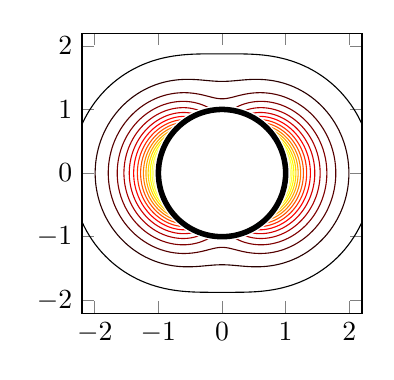
\begin{tikzpicture}

\begin{axis}[%
width=1.4in,
height=1.4in,
at={(0in,0in)},
scale only axis,
colormap/hot2,
xmin=-2.2000,
xmax=2.2000,
ymin=-2.2000,
ymax=2.2000,
axis background/.style={fill=white}
]
\addplot[contour prepared, contour prepared format=matlab, contour/labels=false] table[row sep=crcr] {%
%
0.0556	336.0000\\
2.3637	0.0000\\
2.3619	0.0829\\
2.3564	0.1657\\
2.3545	0.1823\\
2.3473	0.2481\\
2.3346	0.3300\\
2.3183	0.4111\\
2.2984	0.4914\\
2.2930	0.5097\\
2.2751	0.5706\\
2.2484	0.6485\\
2.2322	0.6896\\
2.2183	0.7251\\
2.1849	0.8001\\
2.1722	0.8256\\
2.1484	0.8734\\
2.1129	0.9372\\
2.1087	0.9448\\
2.0661	1.0142\\
2.0542	1.0317\\
2.0205	1.0814\\
1.9962	1.1142\\
1.9722	1.1464\\
1.9389	1.1873\\
1.9213	1.2089\\
1.8822	1.2528\\
1.8679	1.2689\\
1.8261	1.3118\\
1.8121	1.3263\\
1.7706	1.3653\\
1.7540	1.3809\\
1.7157	1.4140\\
1.6940	1.4327\\
1.6613	1.4585\\
1.6320	1.4816\\
1.6075	1.4993\\
1.5683	1.5275\\
1.5542	1.5368\\
1.5029	1.5704\\
1.5016	1.5712\\
1.4490	1.6027\\
1.4363	1.6102\\
1.3969	1.6316\\
1.3684	1.6470\\
1.3453	1.6583\\
1.2994	1.6806\\
1.2943	1.6829\\
1.2432	1.7053\\
1.2296	1.7112\\
1.1924	1.7258\\
1.1590	1.7387\\
1.1419	1.7447\\
1.0918	1.7619\\
1.0880	1.7632\\
1.0412	1.7775\\
1.0166	1.7849\\
0.9909	1.7917\\
0.9450	1.8036\\
0.9409	1.8045\\
0.8900	1.8160\\
0.8735	1.8197\\
0.8389	1.8263\\
0.8021	1.8331\\
0.7876	1.8354\\
0.7357	1.8435\\
0.7309	1.8442\\
0.6821	1.8504\\
0.6602	1.8531\\
0.6273	1.8564\\
0.5899	1.8600\\
0.5710	1.8614\\
0.5203	1.8651\\
0.5121	1.8655\\
0.4512	1.8687\\
0.4495	1.8688\\
0.3829	1.8712\\
0.3805	1.8712\\
0.3152	1.8727\\
0.3004	1.8729\\
0.2480	1.8735\\
0.1982	1.8737\\
0.1814	1.8738\\
0.1153	1.8740\\
0.0493	1.8740\\
-0.0164	1.8740\\
-0.0823	1.8740\\
-0.1483	1.8739\\
-0.1983	1.8737\\
-0.2147	1.8737\\
-0.2815	1.8731\\
-0.3002	1.8729\\
-0.3489	1.8720\\
-0.3793	1.8712\\
-0.4170	1.8701\\
-0.4484	1.8688\\
-0.4857	1.8671\\
-0.5116	1.8655\\
-0.5550	1.8627\\
-0.5710	1.8614\\
-0.6250	1.8567\\
-0.6280	1.8564\\
-0.6822	1.8504\\
-0.6955	1.8489\\
-0.7352	1.8434\\
-0.7665	1.8390\\
-0.7875	1.8354\\
-0.8377	1.8267\\
-0.8394	1.8263\\
-0.8900	1.8160\\
-0.9093	1.8120\\
-0.9405	1.8045\\
-0.9808	1.7946\\
-0.9911	1.7917\\
-1.0414	1.7775\\
-1.0523	1.7744\\
-1.0915	1.7619\\
-1.1236	1.7514\\
-1.1419	1.7447\\
-1.1927	1.7259\\
-1.1944	1.7253\\
-1.2431	1.7053\\
-1.2646	1.6963\\
-1.2940	1.6828\\
-1.3340	1.6642\\
-1.3454	1.6583\\
-1.3971	1.6317\\
-1.4024	1.6290\\
-1.4489	1.6026\\
-1.4698	1.5907\\
-1.5013	1.5710\\
-1.5358	1.5493\\
-1.5542	1.5367\\
-1.6003	1.5049\\
-1.6076	1.4994\\
-1.6615	1.4588\\
-1.6632	1.4575\\
-1.7158	1.4142\\
-1.7242	1.4072\\
-1.7707	1.3654\\
-1.7833	1.3539\\
-1.8261	1.3119\\
-1.8402	1.2979\\
-1.8822	1.2529\\
-1.8949	1.2392\\
-1.9389	1.1875\\
-1.9471	1.1779\\
-1.9963	1.1147\\
-1.9967	1.1142\\
-2.0436	1.0481\\
-2.0542	1.0317\\
-2.0878	0.9797\\
-2.1128	0.9368\\
-2.1289	0.9093\\
-2.1670	0.8369\\
-2.1722	0.8260\\
-2.2020	0.7628\\
-2.2323	0.6905\\
-2.2337	0.6870\\
-2.2622	0.6097\\
-2.2872	0.5311\\
-2.2930	0.5096\\
-2.3088	0.4514\\
-2.3269	0.3706\\
-2.3414	0.2891\\
-2.3523	0.2070\\
-2.3545	0.1813\\
-2.3596	0.1244\\
-2.3632	0.0415\\
-2.3632	-0.0415\\
-2.3596	-0.1244\\
-2.3545	-0.1813\\
-2.3523	-0.2070\\
-2.3414	-0.2891\\
-2.3269	-0.3706\\
-2.3088	-0.4514\\
-2.2930	-0.5096\\
-2.2872	-0.5311\\
-2.2622	-0.6097\\
-2.2337	-0.6870\\
-2.2323	-0.6905\\
-2.2020	-0.7628\\
-2.1722	-0.8260\\
-2.1670	-0.8369\\
-2.1289	-0.9093\\
-2.1128	-0.9368\\
-2.0878	-0.9797\\
-2.0542	-1.0317\\
-2.0436	-1.0481\\
-1.9967	-1.1142\\
-1.9963	-1.1147\\
-1.9471	-1.1779\\
-1.9389	-1.1875\\
-1.8949	-1.2392\\
-1.8822	-1.2529\\
-1.8402	-1.2979\\
-1.8261	-1.3119\\
-1.7833	-1.3539\\
-1.7707	-1.3654\\
-1.7242	-1.4072\\
-1.7158	-1.4142\\
-1.6632	-1.4575\\
-1.6615	-1.4588\\
-1.6076	-1.4994\\
-1.6003	-1.5049\\
-1.5542	-1.5367\\
-1.5358	-1.5493\\
-1.5013	-1.5710\\
-1.4698	-1.5907\\
-1.4489	-1.6026\\
-1.4024	-1.6290\\
-1.3971	-1.6317\\
-1.3454	-1.6583\\
-1.3340	-1.6642\\
-1.2940	-1.6828\\
-1.2646	-1.6963\\
-1.2431	-1.7053\\
-1.1944	-1.7253\\
-1.1927	-1.7259\\
-1.1419	-1.7447\\
-1.1236	-1.7514\\
-1.0915	-1.7619\\
-1.0523	-1.7744\\
-1.0414	-1.7775\\
-0.9911	-1.7917\\
-0.9808	-1.7946\\
-0.9405	-1.8045\\
-0.9093	-1.8120\\
-0.8900	-1.8160\\
-0.8394	-1.8263\\
-0.8377	-1.8267\\
-0.7875	-1.8354\\
-0.7665	-1.8390\\
-0.7352	-1.8434\\
-0.6955	-1.8489\\
-0.6822	-1.8504\\
-0.6280	-1.8564\\
-0.6250	-1.8567\\
-0.5710	-1.8614\\
-0.5550	-1.8627\\
-0.5116	-1.8655\\
-0.4857	-1.8671\\
-0.4484	-1.8688\\
-0.4170	-1.8701\\
-0.3793	-1.8712\\
-0.3489	-1.8720\\
-0.3002	-1.8729\\
-0.2815	-1.8731\\
-0.2147	-1.8737\\
-0.1983	-1.8737\\
-0.1483	-1.8739\\
-0.0823	-1.8740\\
-0.0164	-1.8740\\
0.0493	-1.8740\\
0.1153	-1.8740\\
0.1814	-1.8738\\
0.1982	-1.8737\\
0.2480	-1.8735\\
0.3004	-1.8729\\
0.3152	-1.8727\\
0.3805	-1.8712\\
0.3829	-1.8712\\
0.4495	-1.8688\\
0.4512	-1.8687\\
0.5121	-1.8655\\
0.5203	-1.8651\\
0.5710	-1.8614\\
0.5899	-1.8600\\
0.6273	-1.8564\\
0.6602	-1.8531\\
0.6821	-1.8504\\
0.7309	-1.8442\\
0.7357	-1.8435\\
0.7876	-1.8354\\
0.8021	-1.8331\\
0.8389	-1.8263\\
0.8735	-1.8197\\
0.8900	-1.8160\\
0.9409	-1.8045\\
0.9450	-1.8036\\
0.9909	-1.7917\\
1.0166	-1.7849\\
1.0412	-1.7775\\
1.0880	-1.7632\\
1.0918	-1.7619\\
1.1419	-1.7447\\
1.1590	-1.7387\\
1.1924	-1.7258\\
1.2296	-1.7112\\
1.2432	-1.7053\\
1.2943	-1.6829\\
1.2994	-1.6806\\
1.3453	-1.6583\\
1.3684	-1.6470\\
1.3969	-1.6316\\
1.4363	-1.6102\\
1.4490	-1.6027\\
1.5016	-1.5712\\
1.5029	-1.5704\\
1.5542	-1.5368\\
1.5683	-1.5275\\
1.6075	-1.4993\\
1.6320	-1.4816\\
1.6613	-1.4585\\
1.6940	-1.4327\\
1.7157	-1.4140\\
1.7540	-1.3809\\
1.7706	-1.3653\\
1.8121	-1.3263\\
1.8261	-1.3118\\
1.8679	-1.2689\\
1.8822	-1.2528\\
1.9213	-1.2089\\
1.9389	-1.1873\\
1.9722	-1.1464\\
1.9962	-1.1142\\
2.0205	-1.0814\\
2.0542	-1.0317\\
2.0661	-1.0142\\
2.1087	-0.9448\\
2.1129	-0.9372\\
2.1484	-0.8734\\
2.1722	-0.8256\\
2.1849	-0.8001\\
2.2183	-0.7251\\
2.2322	-0.6896\\
2.2484	-0.6485\\
2.2751	-0.5706\\
2.2930	-0.5097\\
2.2984	-0.4914\\
2.3183	-0.4111\\
2.3346	-0.3300\\
2.3473	-0.2481\\
2.3545	-0.1823\\
2.3564	-0.1657\\
2.3619	-0.0829\\
2.3637	-0.0000\\
0.0556	180.0000\\
0.9932	-0.0000\\
0.9925	-0.0349\\
0.9907	-0.0697\\
0.9877	-0.1044\\
0.9834	-0.1390\\
0.9779	-0.1734\\
0.9712	-0.2076\\
0.9634	-0.2416\\
0.9543	-0.2753\\
0.9441	-0.3086\\
0.9327	-0.3415\\
0.9201	-0.3741\\
0.9064	-0.4061\\
0.8917	-0.4377\\
0.8758	-0.4687\\
0.8588	-0.4992\\
0.8408	-0.5290\\
0.8217	-0.5582\\
0.8016	-0.5867\\
0.7806	-0.6145\\
0.7586	-0.6416\\
0.7356	-0.6678\\
0.7118	-0.6933\\
0.6870	-0.7179\\
0.6615	-0.7416\\
0.6351	-0.7644\\
0.6079	-0.7863\\
0.5800	-0.8072\\
0.5513	-0.8271\\
0.5220	-0.8460\\
0.4921	-0.8639\\
0.4615	-0.8807\\
0.4303	-0.8965\\
0.3987	-0.9112\\
0.3665	-0.9247\\
0.3339	-0.9371\\
0.3008	-0.9484\\
0.2674	-0.9585\\
0.2336	-0.9675\\
0.1995	-0.9752\\
0.1652	-0.9817\\
0.1307	-0.9871\\
0.0960	-0.9911\\
0.0611	-0.9940\\
0.0262	-0.9955\\
-0.0087	-0.9958\\
-0.0437	-0.9949\\
-0.0786	-0.9927\\
-0.1133	-0.9892\\
-0.1480	-0.9846\\
-0.1824	-0.9786\\
-0.2166	-0.9715\\
-0.2505	-0.9632\\
-0.2841	-0.9536\\
-0.3174	-0.9429\\
-0.3502	-0.9311\\
-0.3826	-0.9181\\
-0.4146	-0.9040\\
-0.4460	-0.8888\\
-0.4768	-0.8725\\
-0.5071	-0.8551\\
-0.5368	-0.8367\\
-0.5657	-0.8173\\
-0.5940	-0.7968\\
-0.6216	-0.7754\\
-0.6484	-0.7531\\
-0.6744	-0.7298\\
-0.6995	-0.7057\\
-0.7238	-0.6807\\
-0.7472	-0.6548\\
-0.7697	-0.6282\\
-0.7912	-0.6007\\
-0.8118	-0.5726\\
-0.8314	-0.5437\\
-0.8499	-0.5142\\
-0.8674	-0.4840\\
-0.8838	-0.4533\\
-0.8992	-0.4220\\
-0.9134	-0.3901\\
-0.9265	-0.3578\\
-0.9385	-0.3251\\
-0.9493	-0.2920\\
-0.9590	-0.2585\\
-0.9675	-0.2246\\
-0.9747	-0.1906\\
-0.9808	-0.1562\\
-0.9857	-0.1217\\
-0.9893	-0.0870\\
-0.9918	-0.0523\\
-0.9930	-0.0174\\
-0.9930	0.0174\\
-0.9918	0.0523\\
-0.9893	0.0870\\
-0.9857	0.1217\\
-0.9808	0.1562\\
-0.9747	0.1906\\
-0.9675	0.2246\\
-0.9590	0.2585\\
-0.9493	0.2920\\
-0.9385	0.3251\\
-0.9265	0.3578\\
-0.9134	0.3901\\
-0.8992	0.4220\\
-0.8838	0.4533\\
-0.8674	0.4840\\
-0.8499	0.5142\\
-0.8314	0.5437\\
-0.8118	0.5726\\
-0.7912	0.6007\\
-0.7697	0.6282\\
-0.7472	0.6548\\
-0.7238	0.6807\\
-0.6995	0.7057\\
-0.6744	0.7298\\
-0.6484	0.7531\\
-0.6216	0.7754\\
-0.5940	0.7968\\
-0.5657	0.8173\\
-0.5368	0.8367\\
-0.5071	0.8551\\
-0.4768	0.8725\\
-0.4460	0.8888\\
-0.4146	0.9040\\
-0.3826	0.9181\\
-0.3502	0.9311\\
-0.3174	0.9429\\
-0.2841	0.9536\\
-0.2505	0.9632\\
-0.2166	0.9715\\
-0.1824	0.9786\\
-0.1480	0.9846\\
-0.1133	0.9892\\
-0.0786	0.9927\\
-0.0437	0.9949\\
-0.0087	0.9958\\
0.0262	0.9955\\
0.0611	0.9940\\
0.0960	0.9911\\
0.1307	0.9871\\
0.1652	0.9817\\
0.1995	0.9752\\
0.2336	0.9675\\
0.2674	0.9585\\
0.3008	0.9484\\
0.3339	0.9371\\
0.3665	0.9247\\
0.3987	0.9112\\
0.4303	0.8965\\
0.4615	0.8807\\
0.4921	0.8639\\
0.5220	0.8460\\
0.5513	0.8271\\
0.5800	0.8072\\
0.6079	0.7863\\
0.6351	0.7644\\
0.6615	0.7416\\
0.6870	0.7179\\
0.7118	0.6933\\
0.7356	0.6678\\
0.7586	0.6416\\
0.7806	0.6145\\
0.8016	0.5867\\
0.8217	0.5582\\
0.8408	0.5290\\
0.8588	0.4992\\
0.8758	0.4687\\
0.8917	0.4377\\
0.9064	0.4061\\
0.9201	0.3741\\
0.9327	0.3415\\
0.9441	0.3086\\
0.9543	0.2753\\
0.9634	0.2416\\
0.9712	0.2076\\
0.9779	0.1734\\
0.9834	0.1390\\
0.9877	0.1044\\
0.9907	0.0697\\
0.9925	0.0349\\
0.9932	0.0000\\
0.1111	356.0000\\
1.9939	0.0000\\
1.9923	0.0700\\
1.9875	0.1398\\
1.9795	0.2092\\
1.9683	0.2782\\
1.9558	0.3378\\
1.9540	0.3465\\
1.9366	0.4140\\
1.9162	0.4805\\
1.9031	0.5169\\
1.8927	0.5459\\
1.8663	0.6100\\
1.8512	0.6424\\
1.8371	0.6727\\
1.8050	0.7338\\
1.8000	0.7423\\
1.7703	0.7932\\
1.7496	0.8250\\
1.7330	0.8507\\
1.7000	0.8967\\
1.6931	0.9062\\
1.6510	0.9594\\
1.6509	0.9596\\
1.6064	1.0108\\
1.6028	1.0146\\
1.5597	1.0596\\
1.5552	1.0639\\
1.5111	1.1060\\
1.5084	1.1083\\
1.4622	1.1484\\
1.4605	1.1498\\
1.4166	1.1845\\
1.4083	1.1911\\
1.3717	1.2173\\
1.3544	1.2296\\
1.3274	1.2471\\
1.2991	1.2653\\
1.2838	1.2742\\
1.2424	1.2982\\
1.2409	1.2990\\
1.1983	1.3212\\
1.1847	1.3282\\
1.1564	1.3415\\
1.1261	1.3554\\
1.1151	1.3599\\
1.0744	1.3764\\
1.0666	1.3796\\
1.0339	1.3913\\
1.0066	1.4009\\
0.9942	1.4047\\
0.9550	1.4166\\
0.9461	1.4192\\
0.9159	1.4271\\
0.8853	1.4347\\
0.8776	1.4364\\
0.8395	1.4444\\
0.8244	1.4475\\
0.8017	1.4514\\
0.7647	1.4573\\
0.7637	1.4574\\
0.7272	1.4621\\
0.7032	1.4648\\
0.6905	1.4660\\
0.6538	1.4690\\
0.6431	1.4697\\
0.6171	1.4711\\
0.5835	1.4723\\
0.5810	1.4724\\
0.5440	1.4729\\
0.5247	1.4729\\
0.5073	1.4727\\
0.4706	1.4718\\
0.4668	1.4716\\
0.4325	1.4701\\
0.4097	1.4689\\
0.3942	1.4679\\
0.3552	1.4651\\
0.3537	1.4649\\
0.3132	1.4616\\
0.2988	1.4603\\
0.2687	1.4576\\
0.2449	1.4553\\
0.2198	1.4531\\
0.1920	1.4505\\
0.1617	1.4481\\
0.1400	1.4463\\
0.0888	1.4430\\
0.0763	1.4425\\
0.0379	1.4411\\
-0.0126	1.4407\\
-0.0633	1.4419\\
-0.0762	1.4425\\
-0.1143	1.4445\\
-0.1633	1.4481\\
-0.1659	1.4483\\
-0.2184	1.4528\\
-0.2210	1.4531\\
-0.2697	1.4576\\
-0.2717	1.4578\\
-0.3132	1.4616\\
-0.3261	1.4627\\
-0.3544	1.4651\\
-0.3816	1.4670\\
-0.3943	1.4679\\
-0.4330	1.4702\\
-0.4381	1.4704\\
-0.4701	1.4717\\
-0.4956	1.4725\\
-0.5074	1.4727\\
-0.5442	1.4729\\
-0.5540	1.4729\\
-0.5805	1.4724\\
-0.6132	1.4713\\
-0.6174	1.4711\\
-0.6537	1.4689\\
-0.6731	1.4676\\
-0.6904	1.4660\\
-0.7275	1.4621\\
-0.7334	1.4614\\
-0.7643	1.4572\\
-0.7940	1.4528\\
-0.8019	1.4514\\
-0.8395	1.4444\\
-0.8549	1.4415\\
-0.8775	1.4364\\
-0.9157	1.4273\\
-0.9162	1.4272\\
-0.9548	1.4165\\
-0.9764	1.4104\\
-0.9942	1.4047\\
-1.0342	1.3914\\
-1.0366	1.3906\\
-1.0742	1.3764\\
-1.0964	1.3678\\
-1.1151	1.3598\\
-1.1555	1.3421\\
-1.1566	1.3416\\
-1.1983	1.3212\\
-1.2137	1.3136\\
-1.2407	1.2988\\
-1.2709	1.2821\\
-1.2838	1.2742\\
-1.3269	1.2478\\
-1.3276	1.2473\\
-1.3717	1.2173\\
-1.3815	1.2107\\
-1.4166	1.1844\\
-1.4346	1.1708\\
-1.4621	1.1481\\
-1.4861	1.1283\\
-1.5083	1.1081\\
-1.5357	1.0831\\
-1.5552	1.0637\\
-1.5834	1.0355\\
-1.6027	1.0143\\
-1.6289	0.9855\\
-1.6510	0.9589\\
-1.6723	0.9332\\
-1.6999	0.8965\\
-1.7134	0.8787\\
-1.7497	0.8255\\
-1.7519	0.8221\\
-1.7880	0.7637\\
-1.8000	0.7420\\
-1.8214	0.7035\\
-1.8512	0.6432\\
-1.8520	0.6415\\
-1.8799	0.5782\\
-1.9031	0.5177\\
-1.9048	0.5134\\
-1.9268	0.4474\\
-1.9457	0.3804\\
-1.9558	0.3369\\
-1.9616	0.3124\\
-1.9743	0.2438\\
-1.9839	0.1745\\
-1.9903	0.1049\\
-1.9935	0.0350\\
-1.9935	-0.0350\\
-1.9903	-0.1049\\
-1.9839	-0.1745\\
-1.9743	-0.2438\\
-1.9616	-0.3124\\
-1.9558	-0.3369\\
-1.9457	-0.3804\\
-1.9268	-0.4474\\
-1.9048	-0.5134\\
-1.9031	-0.5177\\
-1.8799	-0.5782\\
-1.8520	-0.6415\\
-1.8512	-0.6432\\
-1.8214	-0.7035\\
-1.8000	-0.7420\\
-1.7880	-0.7637\\
-1.7519	-0.8221\\
-1.7497	-0.8255\\
-1.7134	-0.8787\\
-1.6999	-0.8965\\
-1.6723	-0.9332\\
-1.6510	-0.9589\\
-1.6289	-0.9855\\
-1.6027	-1.0143\\
-1.5834	-1.0355\\
-1.5552	-1.0637\\
-1.5357	-1.0831\\
-1.5083	-1.1081\\
-1.4861	-1.1283\\
-1.4621	-1.1481\\
-1.4346	-1.1708\\
-1.4166	-1.1844\\
-1.3815	-1.2107\\
-1.3717	-1.2173\\
-1.3276	-1.2473\\
-1.3269	-1.2478\\
-1.2838	-1.2742\\
-1.2709	-1.2821\\
-1.2407	-1.2988\\
-1.2137	-1.3136\\
-1.1983	-1.3212\\
-1.1566	-1.3416\\
-1.1555	-1.3421\\
-1.1151	-1.3598\\
-1.0964	-1.3678\\
-1.0742	-1.3764\\
-1.0366	-1.3906\\
-1.0342	-1.3914\\
-0.9942	-1.4047\\
-0.9764	-1.4104\\
-0.9548	-1.4165\\
-0.9162	-1.4272\\
-0.9157	-1.4273\\
-0.8775	-1.4364\\
-0.8549	-1.4415\\
-0.8395	-1.4444\\
-0.8019	-1.4514\\
-0.7940	-1.4528\\
-0.7643	-1.4572\\
-0.7334	-1.4614\\
-0.7275	-1.4621\\
-0.6904	-1.4660\\
-0.6731	-1.4676\\
-0.6537	-1.4689\\
-0.6174	-1.4711\\
-0.6132	-1.4713\\
-0.5805	-1.4724\\
-0.5540	-1.4729\\
-0.5442	-1.4729\\
-0.5074	-1.4727\\
-0.4956	-1.4725\\
-0.4701	-1.4717\\
-0.4381	-1.4704\\
-0.4330	-1.4702\\
-0.3943	-1.4679\\
-0.3816	-1.4670\\
-0.3544	-1.4651\\
-0.3261	-1.4627\\
-0.3132	-1.4616\\
-0.2717	-1.4578\\
-0.2697	-1.4576\\
-0.2210	-1.4531\\
-0.2184	-1.4528\\
-0.1659	-1.4483\\
-0.1633	-1.4481\\
-0.1143	-1.4445\\
-0.0762	-1.4425\\
-0.0633	-1.4419\\
-0.0126	-1.4407\\
0.0379	-1.4411\\
0.0763	-1.4425\\
0.0888	-1.4430\\
0.1400	-1.4463\\
0.1617	-1.4481\\
0.1920	-1.4505\\
0.2198	-1.4531\\
0.2449	-1.4553\\
0.2687	-1.4576\\
0.2988	-1.4603\\
0.3132	-1.4616\\
0.3537	-1.4649\\
0.3552	-1.4651\\
0.3942	-1.4679\\
0.4097	-1.4689\\
0.4325	-1.4701\\
0.4668	-1.4716\\
0.4706	-1.4718\\
0.5073	-1.4727\\
0.5247	-1.4729\\
0.5440	-1.4729\\
0.5810	-1.4724\\
0.5835	-1.4723\\
0.6171	-1.4711\\
0.6431	-1.4697\\
0.6538	-1.4690\\
0.6905	-1.4660\\
0.7032	-1.4648\\
0.7272	-1.4621\\
0.7637	-1.4574\\
0.7647	-1.4573\\
0.8017	-1.4514\\
0.8244	-1.4475\\
0.8395	-1.4444\\
0.8776	-1.4364\\
0.8853	-1.4347\\
0.9159	-1.4271\\
0.9461	-1.4192\\
0.9550	-1.4166\\
0.9942	-1.4047\\
1.0066	-1.4009\\
1.0339	-1.3913\\
1.0666	-1.3796\\
1.0744	-1.3764\\
1.1151	-1.3599\\
1.1261	-1.3554\\
1.1564	-1.3415\\
1.1847	-1.3282\\
1.1983	-1.3212\\
1.2409	-1.2990\\
1.2424	-1.2982\\
1.2838	-1.2742\\
1.2991	-1.2653\\
1.3274	-1.2471\\
1.3544	-1.2296\\
1.3717	-1.2173\\
1.4083	-1.1911\\
1.4166	-1.1845\\
1.4605	-1.1498\\
1.4622	-1.1484\\
1.5084	-1.1083\\
1.5111	-1.1060\\
1.5552	-1.0639\\
1.5597	-1.0596\\
1.6028	-1.0146\\
1.6064	-1.0108\\
1.6509	-0.9596\\
1.6510	-0.9594\\
1.6931	-0.9062\\
1.7000	-0.8967\\
1.7330	-0.8507\\
1.7496	-0.8250\\
1.7703	-0.7932\\
1.8000	-0.7423\\
1.8050	-0.7338\\
1.8371	-0.6727\\
1.8512	-0.6424\\
1.8663	-0.6100\\
1.8927	-0.5459\\
1.9031	-0.5169\\
1.9162	-0.4805\\
1.9366	-0.4140\\
1.9540	-0.3465\\
1.9558	-0.3378\\
1.9683	-0.2782\\
1.9795	-0.2092\\
1.9875	-0.1398\\
1.9923	-0.0700\\
1.9939	-0.0000\\
0.1111	180.0000\\
0.9939	-0.0000\\
0.9932	-0.0349\\
0.9914	-0.0697\\
0.9884	-0.1045\\
0.9841	-0.1391\\
0.9786	-0.1735\\
0.9719	-0.2078\\
0.9641	-0.2418\\
0.9550	-0.2755\\
0.9448	-0.3088\\
0.9334	-0.3418\\
0.9209	-0.3743\\
0.9072	-0.4064\\
0.8924	-0.4381\\
0.8765	-0.4691\\
0.8596	-0.4996\\
0.8415	-0.5295\\
0.8225	-0.5588\\
0.8024	-0.5873\\
0.7814	-0.6152\\
0.7594	-0.6423\\
0.7364	-0.6686\\
0.7126	-0.6941\\
0.6879	-0.7187\\
0.6623	-0.7425\\
0.6359	-0.7654\\
0.6087	-0.7874\\
0.5808	-0.8084\\
0.5522	-0.8284\\
0.5229	-0.8474\\
0.4929	-0.8654\\
0.4624	-0.8824\\
0.4312	-0.8983\\
0.3995	-0.9131\\
0.3673	-0.9268\\
0.3347	-0.9394\\
0.3016	-0.9508\\
0.2681	-0.9611\\
0.2343	-0.9702\\
0.2001	-0.9781\\
0.1657	-0.9848\\
0.1311	-0.9902\\
0.0963	-0.9944\\
0.0613	-0.9973\\
0.0263	-0.9989\\
-0.0088	-0.9993\\
-0.0438	-0.9983\\
-0.0788	-0.9960\\
-0.1137	-0.9925\\
-0.1484	-0.9877\\
-0.1830	-0.9816\\
-0.2172	-0.9743\\
-0.2512	-0.9658\\
-0.2849	-0.9561\\
-0.3182	-0.9452\\
-0.3510	-0.9332\\
-0.3835	-0.9201\\
-0.4154	-0.9058\\
-0.4468	-0.8905\\
-0.4777	-0.8740\\
-0.5080	-0.8566\\
-0.5376	-0.8380\\
-0.5666	-0.8185\\
-0.5949	-0.7980\\
-0.6224	-0.7765\\
-0.6492	-0.7541\\
-0.6752	-0.7307\\
-0.7003	-0.7065\\
-0.7246	-0.6814\\
-0.7480	-0.6555\\
-0.7705	-0.6288\\
-0.7920	-0.6013\\
-0.8126	-0.5731\\
-0.8321	-0.5442\\
-0.8507	-0.5146\\
-0.8682	-0.4844\\
-0.8846	-0.4537\\
-0.8999	-0.4223\\
-0.9142	-0.3905\\
-0.9273	-0.3581\\
-0.9392	-0.3254\\
-0.9500	-0.2922\\
-0.9597	-0.2587\\
-0.9682	-0.2248\\
-0.9754	-0.1907\\
-0.9815	-0.1563\\
-0.9864	-0.1218\\
-0.9900	-0.0871\\
-0.9925	-0.0523\\
-0.9937	-0.0174\\
-0.9937	0.0174\\
-0.9925	0.0523\\
-0.9900	0.0871\\
-0.9864	0.1218\\
-0.9815	0.1563\\
-0.9754	0.1907\\
-0.9682	0.2248\\
-0.9597	0.2587\\
-0.9500	0.2922\\
-0.9392	0.3254\\
-0.9273	0.3581\\
-0.9142	0.3905\\
-0.8999	0.4223\\
-0.8846	0.4537\\
-0.8682	0.4844\\
-0.8507	0.5146\\
-0.8321	0.5442\\
-0.8126	0.5731\\
-0.7920	0.6013\\
-0.7705	0.6288\\
-0.7480	0.6555\\
-0.7246	0.6814\\
-0.7003	0.7065\\
-0.6752	0.7307\\
-0.6492	0.7541\\
-0.6224	0.7765\\
-0.5949	0.7980\\
-0.5666	0.8185\\
-0.5376	0.8380\\
-0.5080	0.8566\\
-0.4777	0.8740\\
-0.4468	0.8905\\
-0.4154	0.9058\\
-0.3835	0.9201\\
-0.3510	0.9332\\
-0.3182	0.9452\\
-0.2849	0.9561\\
-0.2512	0.9658\\
-0.2172	0.9743\\
-0.1830	0.9816\\
-0.1484	0.9877\\
-0.1137	0.9925\\
-0.0788	0.9960\\
-0.0438	0.9983\\
-0.0088	0.9993\\
0.0263	0.9989\\
0.0613	0.9973\\
0.0963	0.9944\\
0.1311	0.9902\\
0.1657	0.9848\\
0.2001	0.9781\\
0.2343	0.9702\\
0.2681	0.9611\\
0.3016	0.9508\\
0.3347	0.9394\\
0.3673	0.9268\\
0.3995	0.9131\\
0.4312	0.8983\\
0.4624	0.8824\\
0.4929	0.8654\\
0.5229	0.8474\\
0.5522	0.8284\\
0.5808	0.8084\\
0.6087	0.7874\\
0.6359	0.7654\\
0.6623	0.7425\\
0.6879	0.7187\\
0.7126	0.6941\\
0.7364	0.6686\\
0.7594	0.6423\\
0.7814	0.6152\\
0.8024	0.5873\\
0.8225	0.5588\\
0.8415	0.5295\\
0.8596	0.4996\\
0.8765	0.4691\\
0.8924	0.4381\\
0.9072	0.4064\\
0.9209	0.3743\\
0.9334	0.3418\\
0.9448	0.3088\\
0.9550	0.2755\\
0.9641	0.2418\\
0.9719	0.2078\\
0.9786	0.1735\\
0.9841	0.1391\\
0.9884	0.1045\\
0.9914	0.0697\\
0.9932	0.0349\\
0.9939	0.0000\\
0.1667	380.0000\\
1.7880	0.0000\\
1.7865	0.0627\\
1.7821	0.1253\\
1.7747	0.1876\\
1.7721	0.2033\\
1.7644	0.2494\\
1.7513	0.3106\\
1.7352	0.3710\\
1.7236	0.4076\\
1.7163	0.4304\\
1.6947	0.4888\\
1.6758	0.5332\\
1.6704	0.5460\\
1.6435	0.6018\\
1.6289	0.6286\\
1.6139	0.6561\\
1.5827	0.7074\\
1.5819	0.7088\\
1.5476	0.7597\\
1.5373	0.7734\\
1.5109	0.8087\\
1.4926	0.8308\\
1.4721	0.8557\\
1.4487	0.8813\\
1.4312	0.9005\\
1.4055	0.9260\\
1.3883	0.9431\\
1.3631	0.9659\\
1.3436	0.9834\\
1.3213	1.0016\\
1.2972	1.0212\\
1.2803	1.0337\\
1.2492	1.0565\\
1.2400	1.0626\\
1.2004	1.0887\\
1.1997	1.0892\\
1.1613	1.1120\\
1.1491	1.1192\\
1.1229	1.1330\\
1.0972	1.1464\\
1.0853	1.1520\\
1.0483	1.1691\\
1.0444	1.1709\\
1.0118	1.1842\\
0.9908	1.1925\\
0.9760	1.1977\\
0.9409	1.2098\\
0.9365	1.2113\\
0.9061	1.2202\\
0.8817	1.2271\\
0.8722	1.2295\\
0.8387	1.2374\\
0.8266	1.2401\\
0.8057	1.2441\\
0.7736	1.2498\\
0.7714	1.2502\\
0.7415	1.2543\\
0.7162	1.2574\\
0.7103	1.2579\\
0.6793	1.2606\\
0.6612	1.2618\\
0.6490	1.2624\\
0.6191	1.2633\\
0.6065	1.2636\\
0.5896	1.2635\\
0.5607	1.2629\\
0.5525	1.2626\\
0.5319	1.2616\\
0.5040	1.2596\\
0.4991	1.2593\\
0.4757	1.2570\\
0.4485	1.2538\\
0.4466	1.2536\\
0.4207	1.2500\\
0.3951	1.2458\\
0.3941	1.2457\\
0.3666	1.2408\\
0.3449	1.2364\\
0.3401	1.2354\\
0.3127	1.2295\\
0.2959	1.2255\\
0.2858	1.2232\\
0.2583	1.2165\\
0.2484	1.2138\\
0.2299	1.2093\\
0.2023	1.2019\\
0.2017	1.2018\\
0.1700	1.1938\\
0.1576	1.1905\\
0.1355	1.1856\\
0.1143	1.1805\\
0.0944	1.1769\\
0.0721	1.1728\\
0.0308	1.1682\\
0.0238	1.1680\\
-0.0102	1.1672\\
-0.0216	1.1680\\
-0.0514	1.1700\\
-0.0931	1.1763\\
-0.0961	1.1769\\
-0.1358	1.1853\\
-0.1369	1.1856\\
-0.1701	1.1938\\
-0.1798	1.1961\\
-0.2007	1.2018\\
-0.2251	1.2079\\
-0.2304	1.2093\\
-0.2581	1.2165\\
-0.2720	1.2198\\
-0.2856	1.2232\\
-0.3130	1.2295\\
-0.3202	1.2311\\
-0.3396	1.2354\\
-0.3671	1.2408\\
-0.3699	1.2413\\
-0.3936	1.2456\\
-0.4207	1.2499\\
-0.4213	1.2500\\
-0.4481	1.2538\\
-0.4727	1.2567\\
-0.4761	1.2570\\
-0.5036	1.2596\\
-0.5257	1.2612\\
-0.5322	1.2616\\
-0.5606	1.2629\\
-0.5794	1.2634\\
-0.5897	1.2635\\
-0.6191	1.2633\\
-0.6338	1.2630\\
-0.6490	1.2624\\
-0.6794	1.2606\\
-0.6886	1.2600\\
-0.7101	1.2579\\
-0.7417	1.2544\\
-0.7438	1.2541\\
-0.7733	1.2497\\
-0.7990	1.2455\\
-0.8058	1.2441\\
-0.8386	1.2374\\
-0.8542	1.2340\\
-0.8721	1.2294\\
-0.9063	1.2203\\
-0.9091	1.2195\\
-0.9407	1.2097\\
-0.9637	1.2023\\
-0.9760	1.1978\\
-1.0119	1.1843\\
-1.0177	1.1821\\
-1.0482	1.1690\\
-1.0709	1.1590\\
-1.0853	1.1520\\
-1.1231	1.1332\\
-1.1232	1.1331\\
-1.1613	1.1120\\
-1.1746	1.1045\\
-1.2003	1.0885\\
-1.2246	1.0732\\
-1.2400	1.0625\\
-1.2733	1.0392\\
-1.2804	1.0338\\
-1.3205	1.0026\\
-1.3215	1.0018\\
-1.3632	0.9661\\
-1.3661	0.9635\\
-1.4056	0.9262\\
-1.4099	0.9221\\
-1.4488	0.8816\\
-1.4519	0.8783\\
-1.4917	0.8324\\
-1.4927	0.8312\\
-1.5295	0.7844\\
-1.5373	0.7735\\
-1.5651	0.7345\\
-1.5827	0.7069\\
-1.5983	0.6827\\
-1.6289	0.6293\\
-1.6290	0.6291\\
-1.6573	0.5741\\
-1.6758	0.5331\\
-1.6829	0.5176\\
-1.7059	0.4598\\
-1.7236	0.4082\\
-1.7261	0.4008\\
-1.7436	0.3409\\
-1.7582	0.2801\\
-1.7699	0.2185\\
-1.7721	0.2033\\
-1.7788	0.1565\\
-1.7847	0.0941\\
-1.7877	0.0314\\
-1.7877	-0.0314\\
-1.7847	-0.0941\\
-1.7788	-0.1565\\
-1.7721	-0.2033\\
-1.7699	-0.2185\\
-1.7582	-0.2801\\
-1.7436	-0.3409\\
-1.7261	-0.4008\\
-1.7236	-0.4082\\
-1.7059	-0.4598\\
-1.6829	-0.5176\\
-1.6758	-0.5331\\
-1.6573	-0.5741\\
-1.6290	-0.6291\\
-1.6289	-0.6293\\
-1.5983	-0.6827\\
-1.5827	-0.7069\\
-1.5651	-0.7345\\
-1.5373	-0.7735\\
-1.5295	-0.7844\\
-1.4927	-0.8312\\
-1.4917	-0.8324\\
-1.4519	-0.8783\\
-1.4488	-0.8816\\
-1.4099	-0.9221\\
-1.4056	-0.9262\\
-1.3661	-0.9635\\
-1.3632	-0.9661\\
-1.3215	-1.0018\\
-1.3205	-1.0026\\
-1.2804	-1.0338\\
-1.2733	-1.0392\\
-1.2400	-1.0625\\
-1.2246	-1.0732\\
-1.2003	-1.0885\\
-1.1746	-1.1045\\
-1.1613	-1.1120\\
-1.1232	-1.1331\\
-1.1231	-1.1332\\
-1.0853	-1.1520\\
-1.0709	-1.1590\\
-1.0482	-1.1690\\
-1.0177	-1.1821\\
-1.0119	-1.1843\\
-0.9760	-1.1978\\
-0.9637	-1.2023\\
-0.9407	-1.2097\\
-0.9091	-1.2195\\
-0.9063	-1.2203\\
-0.8721	-1.2294\\
-0.8542	-1.2340\\
-0.8386	-1.2374\\
-0.8058	-1.2441\\
-0.7990	-1.2455\\
-0.7733	-1.2497\\
-0.7438	-1.2541\\
-0.7417	-1.2544\\
-0.7101	-1.2579\\
-0.6886	-1.2600\\
-0.6794	-1.2606\\
-0.6490	-1.2624\\
-0.6338	-1.2630\\
-0.6191	-1.2633\\
-0.5897	-1.2635\\
-0.5794	-1.2634\\
-0.5606	-1.2629\\
-0.5322	-1.2616\\
-0.5257	-1.2612\\
-0.5036	-1.2596\\
-0.4761	-1.2570\\
-0.4727	-1.2567\\
-0.4481	-1.2538\\
-0.4213	-1.2500\\
-0.4207	-1.2499\\
-0.3936	-1.2456\\
-0.3699	-1.2413\\
-0.3671	-1.2408\\
-0.3396	-1.2354\\
-0.3202	-1.2311\\
-0.3130	-1.2295\\
-0.2856	-1.2232\\
-0.2720	-1.2198\\
-0.2581	-1.2165\\
-0.2304	-1.2093\\
-0.2251	-1.2079\\
-0.2007	-1.2018\\
-0.1798	-1.1961\\
-0.1701	-1.1938\\
-0.1369	-1.1856\\
-0.1358	-1.1853\\
-0.0961	-1.1769\\
-0.0931	-1.1763\\
-0.0514	-1.1700\\
-0.0216	-1.1680\\
-0.0102	-1.1672\\
0.0238	-1.1680\\
0.0308	-1.1682\\
0.0721	-1.1728\\
0.0944	-1.1769\\
0.1143	-1.1805\\
0.1355	-1.1856\\
0.1576	-1.1905\\
0.1700	-1.1938\\
0.2017	-1.2018\\
0.2023	-1.2019\\
0.2299	-1.2093\\
0.2484	-1.2138\\
0.2583	-1.2165\\
0.2858	-1.2232\\
0.2959	-1.2255\\
0.3127	-1.2295\\
0.3401	-1.2354\\
0.3449	-1.2364\\
0.3666	-1.2408\\
0.3941	-1.2457\\
0.3951	-1.2458\\
0.4207	-1.2500\\
0.4466	-1.2536\\
0.4485	-1.2538\\
0.4757	-1.2570\\
0.4991	-1.2593\\
0.5040	-1.2596\\
0.5319	-1.2616\\
0.5525	-1.2626\\
0.5607	-1.2629\\
0.5896	-1.2635\\
0.6065	-1.2636\\
0.6191	-1.2633\\
0.6490	-1.2624\\
0.6612	-1.2618\\
0.6793	-1.2606\\
0.7103	-1.2579\\
0.7162	-1.2574\\
0.7415	-1.2543\\
0.7714	-1.2502\\
0.7736	-1.2498\\
0.8057	-1.2441\\
0.8266	-1.2401\\
0.8387	-1.2374\\
0.8722	-1.2295\\
0.8817	-1.2271\\
0.9061	-1.2202\\
0.9365	-1.2113\\
0.9409	-1.2098\\
0.9760	-1.1977\\
0.9908	-1.1925\\
1.0118	-1.1842\\
1.0444	-1.1709\\
1.0483	-1.1691\\
1.0853	-1.1520\\
1.0972	-1.1464\\
1.1229	-1.1330\\
1.1491	-1.1192\\
1.1613	-1.1120\\
1.1997	-1.0892\\
1.2004	-1.0887\\
1.2400	-1.0626\\
1.2492	-1.0565\\
1.2803	-1.0337\\
1.2972	-1.0212\\
1.3213	-1.0016\\
1.3436	-0.9834\\
1.3631	-0.9659\\
1.3883	-0.9431\\
1.4055	-0.9260\\
1.4312	-0.9005\\
1.4487	-0.8813\\
1.4721	-0.8557\\
1.4926	-0.8308\\
1.5109	-0.8087\\
1.5373	-0.7734\\
1.5476	-0.7597\\
1.5819	-0.7088\\
1.5827	-0.7074\\
1.6139	-0.6561\\
1.6289	-0.6286\\
1.6435	-0.6018\\
1.6704	-0.5460\\
1.6758	-0.5332\\
1.6947	-0.4888\\
1.7163	-0.4304\\
1.7236	-0.4076\\
1.7352	-0.3710\\
1.7513	-0.3106\\
1.7644	-0.2494\\
1.7721	-0.2033\\
1.7747	-0.1876\\
1.7821	-0.1253\\
1.7865	-0.0627\\
1.7880	-0.0000\\
0.1667	180.0000\\
0.9946	-0.0000\\
0.9939	-0.0349\\
0.9921	-0.0698\\
0.9891	-0.1045\\
0.9848	-0.1392\\
0.9793	-0.1737\\
0.9727	-0.2079\\
0.9648	-0.2419\\
0.9557	-0.2757\\
0.9455	-0.3090\\
0.9341	-0.3421\\
0.9216	-0.3746\\
0.9079	-0.4068\\
0.8931	-0.4384\\
0.8773	-0.4695\\
0.8603	-0.5001\\
0.8423	-0.5300\\
0.8233	-0.5593\\
0.8032	-0.5879\\
0.7822	-0.6158\\
0.7602	-0.6429\\
0.7372	-0.6693\\
0.7134	-0.6949\\
0.6887	-0.7196\\
0.6631	-0.7434\\
0.6368	-0.7664\\
0.6096	-0.7885\\
0.5817	-0.8096\\
0.5531	-0.8297\\
0.5238	-0.8488\\
0.4938	-0.8669\\
0.4632	-0.8840\\
0.4321	-0.9001\\
0.4004	-0.9150\\
0.3681	-0.9289\\
0.3355	-0.9416\\
0.3023	-0.9532\\
0.2688	-0.9637\\
0.2349	-0.9729\\
0.2007	-0.9810\\
0.1662	-0.9878\\
0.1315	-0.9934\\
0.0966	-0.9977\\
0.0615	-1.0007\\
0.0264	-1.0023\\
-0.0088	-1.0027\\
-0.0440	-1.0017\\
-0.0791	-0.9993\\
-0.1141	-0.9957\\
-0.1489	-0.9908\\
-0.1835	-0.9846\\
-0.2179	-0.9771\\
-0.2519	-0.9685\\
-0.2856	-0.9586\\
-0.3190	-0.9476\\
-0.3519	-0.9354\\
-0.3843	-0.9221\\
-0.4163	-0.9077\\
-0.4477	-0.8922\\
-0.4786	-0.8756\\
-0.5089	-0.8580\\
-0.5385	-0.8394\\
-0.5675	-0.8197\\
-0.5957	-0.7991\\
-0.6233	-0.7776\\
-0.6500	-0.7550\\
-0.6760	-0.7316\\
-0.7012	-0.7073\\
-0.7254	-0.6822\\
-0.7488	-0.6562\\
-0.7713	-0.6294\\
-0.7928	-0.6019\\
-0.8134	-0.5737\\
-0.8329	-0.5447\\
-0.8514	-0.5151\\
-0.8689	-0.4849\\
-0.8853	-0.4540\\
-0.9007	-0.4227\\
-0.9149	-0.3908\\
-0.9280	-0.3584\\
-0.9400	-0.3256\\
-0.9508	-0.2924\\
-0.9604	-0.2588\\
-0.9689	-0.2250\\
-0.9761	-0.1908\\
-0.9822	-0.1565\\
-0.9871	-0.1219\\
-0.9907	-0.0872\\
-0.9932	-0.0523\\
-0.9944	-0.0175\\
-0.9944	0.0175\\
-0.9932	0.0523\\
-0.9907	0.0872\\
-0.9871	0.1219\\
-0.9822	0.1565\\
-0.9761	0.1908\\
-0.9689	0.2250\\
-0.9604	0.2588\\
-0.9508	0.2924\\
-0.9400	0.3256\\
-0.9280	0.3584\\
-0.9149	0.3908\\
-0.9007	0.4227\\
-0.8853	0.4540\\
-0.8689	0.4849\\
-0.8514	0.5151\\
-0.8329	0.5447\\
-0.8134	0.5737\\
-0.7928	0.6019\\
-0.7713	0.6294\\
-0.7488	0.6562\\
-0.7254	0.6822\\
-0.7012	0.7073\\
-0.6760	0.7316\\
-0.6500	0.7550\\
-0.6233	0.7776\\
-0.5957	0.7991\\
-0.5675	0.8197\\
-0.5385	0.8394\\
-0.5089	0.8580\\
-0.4786	0.8756\\
-0.4477	0.8922\\
-0.4163	0.9077\\
-0.3843	0.9221\\
-0.3519	0.9354\\
-0.3190	0.9476\\
-0.2856	0.9586\\
-0.2519	0.9685\\
-0.2179	0.9771\\
-0.1835	0.9846\\
-0.1489	0.9908\\
-0.1141	0.9957\\
-0.0791	0.9993\\
-0.0440	1.0017\\
-0.0088	1.0027\\
0.0264	1.0023\\
0.0615	1.0007\\
0.0966	0.9977\\
0.1315	0.9934\\
0.1662	0.9878\\
0.2007	0.9810\\
0.2349	0.9729\\
0.2688	0.9637\\
0.3023	0.9532\\
0.3355	0.9416\\
0.3681	0.9289\\
0.4004	0.9150\\
0.4321	0.9001\\
0.4632	0.8840\\
0.4938	0.8669\\
0.5238	0.8488\\
0.5531	0.8297\\
0.5817	0.8096\\
0.6096	0.7885\\
0.6368	0.7664\\
0.6631	0.7434\\
0.6887	0.7196\\
0.7134	0.6949\\
0.7372	0.6693\\
0.7602	0.6429\\
0.7822	0.6158\\
0.8032	0.5879\\
0.8233	0.5593\\
0.8423	0.5300\\
0.8603	0.5001\\
0.8773	0.4695\\
0.8931	0.4384\\
0.9079	0.4068\\
0.9216	0.3746\\
0.9341	0.3421\\
0.9455	0.3090\\
0.9557	0.2757\\
0.9648	0.2419\\
0.9727	0.2079\\
0.9793	0.1737\\
0.9848	0.1392\\
0.9891	0.1045\\
0.9921	0.0698\\
0.9939	0.0349\\
0.9946	0.0000\\
0.2222	134.0000\\
1.6474	0.0000\\
1.6460	0.0578\\
1.6418	0.1154\\
1.6414	0.1184\\
1.6348	0.1728\\
1.6252	0.2297\\
1.6127	0.2860\\
1.5976	0.3415\\
1.5957	0.3474\\
1.5799	0.3962\\
1.5595	0.4498\\
1.5508	0.4698\\
1.5366	0.5023\\
1.5112	0.5534\\
1.5066	0.5616\\
1.4835	0.6031\\
1.4633	0.6353\\
1.4534	0.6512\\
1.4210	0.6975\\
1.4208	0.6978\\
1.3865	0.7421\\
1.3790	0.7509\\
1.3500	0.7847\\
1.3380	0.7975\\
1.3116	0.8253\\
1.2977	0.8385\\
1.2713	0.8636\\
1.2582	0.8749\\
1.2292	0.8997\\
1.2194	0.9074\\
1.1856	0.9334\\
1.1813	0.9364\\
1.1440	0.9623\\
1.1406	0.9647\\
1.1073	0.9853\\
1.0942	0.9934\\
1.0713	1.0060\\
1.0466	1.0194\\
1.0361	1.0246\\
1.0016	1.0411\\
0.9980	1.0428\\
0.9675	1.0557\\
0.9485	1.0634\\
0.9343	1.0686\\
0.9018	1.0800\\
0.8983	1.0812\\
0.8697	1.0898\\
0.8475	1.0961\\
0.8384	1.0984\\
0.8077	1.1056\\
0.7962	1.1082\\
0.7775	1.1117\\
0.7482	1.1167\\
0.7447	1.1172\\
0.7192	1.1205\\
0.6931	1.1234\\
0.6911	1.1235\\
0.6632	1.1255\\
0.6416	1.1265\\
0.6363	1.1266\\
0.6095	1.1269\\
0.5904	1.1267\\
0.5837	1.1265\\
0.5581	1.1253\\
0.5395	1.1240\\
0.5334	1.1234\\
0.5089	1.1209\\
0.4893	1.1183\\
0.4853	1.1177\\
0.4618	1.1139\\
0.4398	1.1097\\
0.4394	1.1096\\
0.4167	1.1048\\
0.3952	1.0994\\
0.3913	1.0984\\
0.3736	1.0936\\
0.3529	1.0873\\
0.3439	1.0843\\
0.3325	1.0805\\
0.3125	1.0734\\
0.2978	1.0676\\
0.2933	1.0658\\
0.2739	1.0579\\
0.2557	1.0497\\
0.2532	1.0484\\
0.2370	1.0411\\
0.2193	1.0321\\
0.2102	1.0272\\
0.2017	1.0229\\
0.1842	1.0134\\
0.1690	1.0042\\
0.1679	1.0036\\
0.1502	0.9936\\
0.1668	0.9909\\
0.2013	0.9839\\
0.2356	0.9757\\
0.2695	0.9662\\
0.3031	0.9556\\
0.3363	0.9439\\
0.3690	0.9310\\
0.4012	0.9169\\
0.4329	0.9018\\
0.4641	0.8857\\
0.4947	0.8685\\
0.5246	0.8502\\
0.5539	0.8310\\
0.5825	0.8108\\
0.6104	0.7896\\
0.6376	0.7674\\
0.6640	0.7444\\
0.6895	0.7205\\
0.7142	0.6957\\
0.7380	0.6700\\
0.7610	0.6436\\
0.7830	0.6164\\
0.8040	0.5885\\
0.8240	0.5598\\
0.8431	0.5305\\
0.8611	0.5005\\
0.8780	0.4699\\
0.8939	0.4388\\
0.9087	0.4071\\
0.9223	0.3749\\
0.9348	0.3423\\
0.9462	0.3093\\
0.9564	0.2759\\
0.9655	0.2421\\
0.9734	0.2081\\
0.9800	0.1738\\
0.9855	0.1393\\
0.9898	0.1046\\
0.9928	0.0698\\
0.9946	0.0349\\
0.9953	0.0000\\
0.2222	134.0000\\
0.9953	-0.0000\\
0.9946	-0.0349\\
0.9928	-0.0698\\
0.9898	-0.1046\\
0.9855	-0.1393\\
0.9800	-0.1738\\
0.9734	-0.2081\\
0.9655	-0.2421\\
0.9564	-0.2759\\
0.9462	-0.3093\\
0.9348	-0.3423\\
0.9223	-0.3749\\
0.9087	-0.4071\\
0.8939	-0.4388\\
0.8780	-0.4699\\
0.8611	-0.5005\\
0.8431	-0.5305\\
0.8240	-0.5598\\
0.8040	-0.5885\\
0.7830	-0.6164\\
0.7610	-0.6436\\
0.7380	-0.6700\\
0.7142	-0.6957\\
0.6895	-0.7205\\
0.6640	-0.7444\\
0.6376	-0.7674\\
0.6104	-0.7896\\
0.5825	-0.8108\\
0.5539	-0.8310\\
0.5246	-0.8502\\
0.4947	-0.8685\\
0.4641	-0.8857\\
0.4329	-0.9018\\
0.4012	-0.9169\\
0.3690	-0.9310\\
0.3363	-0.9439\\
0.3031	-0.9556\\
0.2695	-0.9662\\
0.2356	-0.9757\\
0.2013	-0.9839\\
0.1668	-0.9909\\
0.1502	-0.9936\\
0.1679	-1.0036\\
0.1690	-1.0042\\
0.1842	-1.0134\\
0.2017	-1.0229\\
0.2102	-1.0272\\
0.2193	-1.0321\\
0.2370	-1.0411\\
0.2532	-1.0484\\
0.2557	-1.0497\\
0.2739	-1.0579\\
0.2933	-1.0658\\
0.2978	-1.0676\\
0.3125	-1.0734\\
0.3325	-1.0805\\
0.3439	-1.0843\\
0.3529	-1.0873\\
0.3736	-1.0936\\
0.3913	-1.0984\\
0.3952	-1.0994\\
0.4167	-1.1048\\
0.4394	-1.1096\\
0.4398	-1.1097\\
0.4618	-1.1139\\
0.4853	-1.1177\\
0.4893	-1.1183\\
0.5089	-1.1209\\
0.5334	-1.1234\\
0.5395	-1.1240\\
0.5581	-1.1253\\
0.5837	-1.1265\\
0.5904	-1.1267\\
0.6095	-1.1269\\
0.6363	-1.1266\\
0.6416	-1.1265\\
0.6632	-1.1255\\
0.6911	-1.1235\\
0.6931	-1.1234\\
0.7192	-1.1205\\
0.7447	-1.1172\\
0.7482	-1.1167\\
0.7775	-1.1117\\
0.7962	-1.1082\\
0.8077	-1.1056\\
0.8384	-1.0984\\
0.8475	-1.0961\\
0.8697	-1.0898\\
0.8983	-1.0812\\
0.9018	-1.0800\\
0.9343	-1.0686\\
0.9485	-1.0634\\
0.9675	-1.0557\\
0.9980	-1.0428\\
1.0016	-1.0411\\
1.0361	-1.0246\\
1.0466	-1.0194\\
1.0713	-1.0060\\
1.0942	-0.9934\\
1.1073	-0.9853\\
1.1406	-0.9647\\
1.1440	-0.9623\\
1.1813	-0.9364\\
1.1856	-0.9334\\
1.2194	-0.9074\\
1.2292	-0.8997\\
1.2582	-0.8749\\
1.2713	-0.8636\\
1.2977	-0.8385\\
1.3116	-0.8253\\
1.3380	-0.7975\\
1.3500	-0.7847\\
1.3790	-0.7509\\
1.3865	-0.7421\\
1.4208	-0.6978\\
1.4210	-0.6975\\
1.4534	-0.6512\\
1.4633	-0.6353\\
1.4835	-0.6031\\
1.5066	-0.5616\\
1.5112	-0.5534\\
1.5366	-0.5023\\
1.5508	-0.4698\\
1.5595	-0.4498\\
1.5799	-0.3962\\
1.5957	-0.3474\\
1.5976	-0.3415\\
1.6127	-0.2860\\
1.6252	-0.2297\\
1.6348	-0.1728\\
1.6414	-0.1184\\
1.6418	-0.1154\\
1.6460	-0.0578\\
1.6474	-0.0000\\
0.2222	265.0000\\
-0.1841	0.9875\\
-0.1510	0.9936\\
-0.1671	1.0036\\
-0.1846	1.0134\\
-0.1894	1.0159\\
-0.2016	1.0229\\
-0.2191	1.0321\\
-0.2315	1.0380\\
-0.2373	1.0411\\
-0.2552	1.0497\\
-0.2745	1.0579\\
-0.2753	1.0583\\
-0.2930	1.0658\\
-0.3127	1.0734\\
-0.3207	1.0762\\
-0.3325	1.0805\\
-0.3528	1.0873\\
-0.3675	1.0917\\
-0.3738	1.0936\\
-0.3949	1.0994\\
-0.4154	1.1044\\
-0.4171	1.1048\\
-0.4390	1.1096\\
-0.4621	1.1140\\
-0.4645	1.1144\\
-0.4851	1.1177\\
-0.5091	1.1209\\
-0.5143	1.1215\\
-0.5332	1.1234\\
-0.5583	1.1253\\
-0.5649	1.1257\\
-0.5836	1.1265\\
-0.6097	1.1270\\
-0.6160	1.1270\\
-0.6361	1.1266\\
-0.6634	1.1255\\
-0.6674	1.1253\\
-0.6909	1.1235\\
-0.7189	1.1207\\
-0.7194	1.1206\\
-0.7480	1.1166\\
-0.7705	1.1131\\
-0.7777	1.1117\\
-0.8077	1.1056\\
-0.8219	1.1025\\
-0.8383	1.0983\\
-0.8698	1.0899\\
-0.8729	1.0890\\
-0.9016	1.0799\\
-0.9235	1.0727\\
-0.9343	1.0686\\
-0.9676	1.0557\\
-0.9734	1.0535\\
-1.0014	1.0410\\
-1.0225	1.0315\\
-1.0361	1.0246\\
-1.0705	1.0067\\
-1.0714	1.0062\\
-1.1073	0.9854\\
-1.1176	0.9793\\
-1.1439	0.9622\\
-1.1633	0.9494\\
-1.1813	0.9363\\
-1.2076	0.9169\\
-1.2194	0.9073\\
-1.2504	0.8819\\
-1.2582	0.8750\\
-1.2916	0.8447\\
-1.2977	0.8386\\
-1.3310	0.8052\\
-1.3380	0.7975\\
-1.3685	0.7637\\
-1.3790	0.7509\\
-1.4041	0.7201\\
-1.4207	0.6974\\
-1.4375	0.6746\\
-1.4633	0.6355\\
-1.4687	0.6273\\
-1.4977	0.5784\\
-1.5066	0.5614\\
-1.5242	0.5280\\
-1.5484	0.4762\\
-1.5508	0.4703\\
-1.5700	0.4231\\
-1.5891	0.3690\\
-1.5957	0.3468\\
-1.6055	0.3139\\
-1.6193	0.2579\\
-1.6304	0.2013\\
-1.6387	0.1442\\
-1.6414	0.1155\\
-1.6442	0.0867\\
-1.6470	0.0289\\
-1.6470	-0.0289\\
-1.6442	-0.0867\\
-1.6414	-0.1155\\
-1.6387	-0.1442\\
-1.6304	-0.2013\\
-1.6193	-0.2579\\
-1.6055	-0.3139\\
-1.5957	-0.3468\\
-1.5891	-0.3690\\
-1.5700	-0.4231\\
-1.5508	-0.4703\\
-1.5484	-0.4762\\
-1.5242	-0.5280\\
-1.5066	-0.5614\\
-1.4977	-0.5784\\
-1.4687	-0.6273\\
-1.4633	-0.6355\\
-1.4375	-0.6746\\
-1.4207	-0.6974\\
-1.4041	-0.7201\\
-1.3790	-0.7509\\
-1.3685	-0.7637\\
-1.3380	-0.7975\\
-1.3310	-0.8052\\
-1.2977	-0.8386\\
-1.2916	-0.8447\\
-1.2582	-0.8750\\
-1.2504	-0.8819\\
-1.2194	-0.9073\\
-1.2076	-0.9169\\
-1.1813	-0.9363\\
-1.1633	-0.9494\\
-1.1439	-0.9622\\
-1.1176	-0.9793\\
-1.1073	-0.9854\\
-1.0714	-1.0062\\
-1.0705	-1.0067\\
-1.0361	-1.0246\\
-1.0225	-1.0315\\
-1.0014	-1.0410\\
-0.9734	-1.0535\\
-0.9676	-1.0557\\
-0.9343	-1.0686\\
-0.9235	-1.0727\\
-0.9016	-1.0799\\
-0.8729	-1.0890\\
-0.8698	-1.0899\\
-0.8383	-1.0983\\
-0.8219	-1.1025\\
-0.8077	-1.1056\\
-0.7777	-1.1117\\
-0.7705	-1.1131\\
-0.7480	-1.1166\\
-0.7194	-1.1206\\
-0.7189	-1.1207\\
-0.6909	-1.1235\\
-0.6674	-1.1253\\
-0.6634	-1.1255\\
-0.6361	-1.1266\\
-0.6160	-1.1270\\
-0.6097	-1.1270\\
-0.5836	-1.1265\\
-0.5649	-1.1257\\
-0.5583	-1.1253\\
-0.5332	-1.1234\\
-0.5143	-1.1215\\
-0.5091	-1.1209\\
-0.4851	-1.1177\\
-0.4645	-1.1144\\
-0.4621	-1.1140\\
-0.4390	-1.1096\\
-0.4171	-1.1048\\
-0.4154	-1.1044\\
-0.3949	-1.0994\\
-0.3738	-1.0936\\
-0.3675	-1.0917\\
-0.3528	-1.0873\\
-0.3325	-1.0805\\
-0.3207	-1.0762\\
-0.3127	-1.0734\\
-0.2930	-1.0658\\
-0.2753	-1.0583\\
-0.2745	-1.0579\\
-0.2552	-1.0497\\
-0.2373	-1.0411\\
-0.2315	-1.0380\\
-0.2191	-1.0321\\
-0.2016	-1.0229\\
-0.1894	-1.0159\\
-0.1846	-1.0134\\
-0.1671	-1.0036\\
-0.1510	-0.9936\\
-0.1841	-0.9875\\
-0.2185	-0.9799\\
-0.2526	-0.9711\\
-0.2864	-0.9611\\
-0.3197	-0.9499\\
-0.3527	-0.9375\\
-0.3851	-0.9241\\
-0.4171	-0.9095\\
-0.4486	-0.8939\\
-0.4794	-0.8772\\
-0.5097	-0.8595\\
-0.5394	-0.8407\\
-0.5683	-0.8210\\
-0.5966	-0.8003\\
-0.6241	-0.7786\\
-0.6509	-0.7560\\
-0.6768	-0.7325\\
-0.7020	-0.7082\\
-0.7262	-0.6829\\
-0.7496	-0.6569\\
-0.7721	-0.6301\\
-0.7936	-0.6025\\
-0.8141	-0.5742\\
-0.8337	-0.5452\\
-0.8522	-0.5156\\
-0.8697	-0.4853\\
-0.8861	-0.4544\\
-0.9014	-0.4230\\
-0.9156	-0.3911\\
-0.9287	-0.3587\\
-0.9407	-0.3259\\
-0.9515	-0.2926\\
-0.9611	-0.2590\\
-0.9696	-0.2251\\
-0.9768	-0.1910\\
-0.9829	-0.1566\\
-0.9878	-0.1220\\
-0.9914	-0.0872\\
-0.9939	-0.0524\\
-0.9951	-0.0175\\
-0.9951	0.0175\\
-0.9939	0.0524\\
-0.9914	0.0872\\
-0.9878	0.1220\\
-0.9829	0.1566\\
-0.9768	0.1910\\
-0.9696	0.2251\\
-0.9611	0.2590\\
-0.9515	0.2926\\
-0.9407	0.3259\\
-0.9287	0.3587\\
-0.9156	0.3911\\
-0.9014	0.4230\\
-0.8861	0.4544\\
-0.8697	0.4853\\
-0.8522	0.5156\\
-0.8337	0.5452\\
-0.8141	0.5742\\
-0.7936	0.6025\\
-0.7721	0.6301\\
-0.7496	0.6569\\
-0.7262	0.6829\\
-0.7020	0.7082\\
-0.6768	0.7325\\
-0.6509	0.7560\\
-0.6241	0.7786\\
-0.5966	0.8003\\
-0.5683	0.8210\\
-0.5394	0.8407\\
-0.5097	0.8595\\
-0.4794	0.8772\\
-0.4486	0.8939\\
-0.4171	0.9095\\
-0.3851	0.9241\\
-0.3527	0.9375\\
-0.3197	0.9499\\
-0.2864	0.9611\\
-0.2526	0.9711\\
-0.2185	0.9799\\
-0.1841	0.9875\\
0.2778	115.0000\\
1.5417	0.0000\\
1.5404	0.0541\\
1.5364	0.1080\\
1.5298	0.1617\\
1.5205	0.2149\\
1.5103	0.2604\\
1.5087	0.2675\\
1.4943	0.3195\\
1.4774	0.3705\\
1.4672	0.3967\\
1.4580	0.4205\\
1.4362	0.4694\\
1.4249	0.4916\\
1.4120	0.5170\\
1.3855	0.5632\\
1.3834	0.5664\\
1.3569	0.6079\\
1.3427	0.6276\\
1.3261	0.6509\\
1.3028	0.6801\\
1.2932	0.6922\\
1.2637	0.7255\\
1.2584	0.7315\\
1.2254	0.7651\\
1.2218	0.7688\\
1.1878	0.8000\\
1.1834	0.8040\\
1.1509	0.8308\\
1.1435	0.8369\\
1.1148	0.8582\\
1.1020	0.8676\\
1.0794	0.8826\\
1.0592	0.8958\\
1.0447	0.9043\\
1.0150	0.9215\\
1.0108	0.9237\\
0.9775	0.9407\\
0.9698	0.9446\\
0.9449	0.9558\\
0.9236	0.9651\\
0.9131	0.9691\\
0.8819	0.9808\\
0.8766	0.9828\\
0.8513	0.9908\\
0.8289	0.9977\\
0.8216	0.9996\\
0.7923	1.0069\\
0.7806	1.0097\\
0.7638	1.0130\\
0.7360	1.0180\\
0.7320	1.0187\\
0.7086	1.0219\\
0.6831	1.0248\\
0.6822	1.0249\\
0.6560	1.0268\\
0.6342	1.0278\\
0.6308	1.0279\\
0.6058	1.0281\\
0.5854	1.0277\\
0.5819	1.0275\\
0.5581	1.0262\\
0.5368	1.0244\\
0.5354	1.0243\\
0.5128	1.0216\\
0.4913	1.0183\\
0.4886	1.0178\\
0.4699	1.0144\\
0.4494	1.0100\\
0.4410	1.0079\\
0.4293	1.0050\\
0.4098	0.9995\\
0.3942	0.9945\\
0.3912	0.9936\\
0.3726	0.9871\\
0.3551	0.9803\\
0.3482	0.9774\\
0.3379	0.9731\\
0.3212	0.9654\\
0.3055	0.9574\\
0.3371	0.9461\\
0.3698	0.9330\\
0.4020	0.9189\\
0.4338	0.9036\\
0.4649	0.8873\\
0.4955	0.8700\\
0.5255	0.8516\\
0.5548	0.8323\\
0.5834	0.8119\\
0.6113	0.7907\\
0.6384	0.7684\\
0.6648	0.7453\\
0.6903	0.7213\\
0.7150	0.6965\\
0.7389	0.6708\\
0.7618	0.6443\\
0.7837	0.6170\\
0.8048	0.5890\\
0.8248	0.5603\\
0.8438	0.5309\\
0.8618	0.5009\\
0.8788	0.4703\\
0.8946	0.4391\\
0.9094	0.4074\\
0.9230	0.3752\\
0.9356	0.3426\\
0.9469	0.3095\\
0.9572	0.2761\\
0.9662	0.2423\\
0.9741	0.2082\\
0.9807	0.1739\\
0.9862	0.1394\\
0.9905	0.1047\\
0.9935	0.0699\\
0.9953	0.0350\\
0.9960	0.0000\\
0.2778	115.0000\\
0.9960	-0.0000\\
0.9953	-0.0350\\
0.9935	-0.0699\\
0.9905	-0.1047\\
0.9862	-0.1394\\
0.9807	-0.1739\\
0.9741	-0.2082\\
0.9662	-0.2423\\
0.9572	-0.2761\\
0.9469	-0.3095\\
0.9356	-0.3426\\
0.9230	-0.3752\\
0.9094	-0.4074\\
0.8946	-0.4391\\
0.8788	-0.4703\\
0.8618	-0.5009\\
0.8438	-0.5309\\
0.8248	-0.5603\\
0.8048	-0.5890\\
0.7837	-0.6170\\
0.7618	-0.6443\\
0.7389	-0.6708\\
0.7150	-0.6965\\
0.6903	-0.7213\\
0.6648	-0.7453\\
0.6384	-0.7684\\
0.6113	-0.7907\\
0.5834	-0.8119\\
0.5548	-0.8323\\
0.5255	-0.8516\\
0.4955	-0.8700\\
0.4649	-0.8873\\
0.4338	-0.9036\\
0.4020	-0.9189\\
0.3698	-0.9330\\
0.3371	-0.9461\\
0.3055	-0.9574\\
0.3212	-0.9654\\
0.3379	-0.9731\\
0.3482	-0.9774\\
0.3551	-0.9803\\
0.3726	-0.9871\\
0.3912	-0.9936\\
0.3942	-0.9945\\
0.4098	-0.9995\\
0.4293	-1.0050\\
0.4410	-1.0079\\
0.4494	-1.0100\\
0.4699	-1.0144\\
0.4886	-1.0178\\
0.4913	-1.0183\\
0.5128	-1.0216\\
0.5354	-1.0243\\
0.5368	-1.0244\\
0.5581	-1.0262\\
0.5819	-1.0275\\
0.5854	-1.0277\\
0.6058	-1.0281\\
0.6308	-1.0279\\
0.6342	-1.0278\\
0.6560	-1.0268\\
0.6822	-1.0249\\
0.6831	-1.0248\\
0.7086	-1.0219\\
0.7320	-1.0187\\
0.7360	-1.0180\\
0.7638	-1.0130\\
0.7806	-1.0097\\
0.7923	-1.0069\\
0.8216	-0.9996\\
0.8289	-0.9977\\
0.8513	-0.9908\\
0.8766	-0.9828\\
0.8819	-0.9808\\
0.9131	-0.9691\\
0.9236	-0.9651\\
0.9449	-0.9558\\
0.9698	-0.9446\\
0.9775	-0.9407\\
1.0108	-0.9237\\
1.0150	-0.9215\\
1.0447	-0.9043\\
1.0592	-0.8958\\
1.0794	-0.8826\\
1.1020	-0.8676\\
1.1148	-0.8582\\
1.1435	-0.8369\\
1.1509	-0.8308\\
1.1834	-0.8040\\
1.1878	-0.8000\\
1.2218	-0.7688\\
1.2254	-0.7651\\
1.2584	-0.7315\\
1.2637	-0.7255\\
1.2932	-0.6922\\
1.3028	-0.6801\\
1.3261	-0.6509\\
1.3427	-0.6276\\
1.3569	-0.6079\\
1.3834	-0.5664\\
1.3855	-0.5632\\
1.4120	-0.5170\\
1.4249	-0.4916\\
1.4362	-0.4694\\
1.4580	-0.4205\\
1.4672	-0.3967\\
1.4774	-0.3705\\
1.4943	-0.3195\\
1.5087	-0.2675\\
1.5103	-0.2604\\
1.5205	-0.2149\\
1.5298	-0.1617\\
1.5364	-0.1080\\
1.5404	-0.0541\\
1.5417	-0.0000\\
0.2778	231.0000\\
-0.3205	0.9522\\
-0.3051	0.9574\\
-0.3214	0.9654\\
-0.3256	0.9674\\
-0.3378	0.9730\\
-0.3549	0.9803\\
-0.3711	0.9864\\
-0.3730	0.9871\\
-0.3909	0.9935\\
-0.4100	0.9995\\
-0.4175	1.0017\\
-0.4293	1.0050\\
-0.4493	1.0099\\
-0.4647	1.0133\\
-0.4701	1.0144\\
-0.4910	1.0183\\
-0.5126	1.0215\\
-0.5131	1.0216\\
-0.5352	1.0242\\
-0.5583	1.0262\\
-0.5610	1.0265\\
-0.5817	1.0275\\
-0.6060	1.0281\\
-0.6098	1.0282\\
-0.6306	1.0278\\
-0.6562	1.0268\\
-0.6587	1.0267\\
-0.6820	1.0248\\
-0.7076	1.0221\\
-0.7088	1.0220\\
-0.7358	1.0180\\
-0.7564	1.0146\\
-0.7638	1.0130\\
-0.7923	1.0069\\
-0.8048	1.0040\\
-0.8215	0.9995\\
-0.8515	0.9909\\
-0.8528	0.9905\\
-0.8819	0.9807\\
-0.9002	0.9743\\
-0.9131	0.9691\\
-0.9450	0.9559\\
-0.9468	0.9552\\
-0.9775	0.9407\\
-0.9926	0.9334\\
-1.0107	0.9236\\
-1.0372	0.9090\\
-1.0447	0.9044\\
-1.0795	0.8828\\
-1.0807	0.8820\\
-1.1148	0.8583\\
-1.1229	0.8525\\
-1.1509	0.8308\\
-1.1637	0.8207\\
-1.1877	0.7998\\
-1.2029	0.7867\\
-1.2253	0.7649\\
-1.2404	0.7504\\
-1.2637	0.7253\\
-1.2761	0.7121\\
-1.3028	0.6801\\
-1.3099	0.6718\\
-1.3417	0.6296\\
-1.3428	0.6280\\
-1.3715	0.5858\\
-1.3834	0.5661\\
-1.3990	0.5403\\
-1.4243	0.4934\\
-1.4249	0.4922\\
-1.4474	0.4451\\
-1.4672	0.3975\\
-1.4679	0.3956\\
-1.4862	0.3451\\
-1.5018	0.2936\\
-1.5103	0.2598\\
-1.5149	0.2413\\
-1.5255	0.1884\\
-1.5334	0.1349\\
-1.5387	0.0811\\
-1.5414	0.0271\\
-1.5414	-0.0271\\
-1.5387	-0.0811\\
-1.5334	-0.1349\\
-1.5255	-0.1884\\
-1.5149	-0.2413\\
-1.5103	-0.2598\\
-1.5018	-0.2936\\
-1.4862	-0.3451\\
-1.4679	-0.3956\\
-1.4672	-0.3975\\
-1.4474	-0.4451\\
-1.4249	-0.4922\\
-1.4243	-0.4934\\
-1.3990	-0.5403\\
-1.3834	-0.5661\\
-1.3715	-0.5858\\
-1.3428	-0.6280\\
-1.3417	-0.6296\\
-1.3099	-0.6718\\
-1.3028	-0.6801\\
-1.2761	-0.7121\\
-1.2637	-0.7253\\
-1.2404	-0.7504\\
-1.2253	-0.7649\\
-1.2029	-0.7867\\
-1.1877	-0.7998\\
-1.1637	-0.8207\\
-1.1509	-0.8308\\
-1.1229	-0.8525\\
-1.1148	-0.8583\\
-1.0807	-0.8820\\
-1.0795	-0.8828\\
-1.0447	-0.9044\\
-1.0372	-0.9090\\
-1.0107	-0.9236\\
-0.9926	-0.9334\\
-0.9775	-0.9407\\
-0.9468	-0.9552\\
-0.9450	-0.9559\\
-0.9131	-0.9691\\
-0.9002	-0.9743\\
-0.8819	-0.9807\\
-0.8528	-0.9905\\
-0.8515	-0.9909\\
-0.8215	-0.9995\\
-0.8048	-1.0040\\
-0.7923	-1.0069\\
-0.7638	-1.0130\\
-0.7564	-1.0146\\
-0.7358	-1.0180\\
-0.7088	-1.0220\\
-0.7076	-1.0221\\
-0.6820	-1.0248\\
-0.6587	-1.0267\\
-0.6562	-1.0268\\
-0.6306	-1.0278\\
-0.6098	-1.0282\\
-0.6060	-1.0281\\
-0.5817	-1.0275\\
-0.5610	-1.0265\\
-0.5583	-1.0262\\
-0.5352	-1.0242\\
-0.5131	-1.0216\\
-0.5126	-1.0215\\
-0.4910	-1.0183\\
-0.4701	-1.0144\\
-0.4647	-1.0133\\
-0.4493	-1.0099\\
-0.4293	-1.0050\\
-0.4175	-1.0017\\
-0.4100	-0.9995\\
-0.3909	-0.9935\\
-0.3730	-0.9871\\
-0.3711	-0.9864\\
-0.3549	-0.9803\\
-0.3378	-0.9730\\
-0.3256	-0.9674\\
-0.3214	-0.9654\\
-0.3051	-0.9574\\
-0.3205	-0.9522\\
-0.3535	-0.9397\\
-0.3860	-0.9261\\
-0.4180	-0.9114\\
-0.4494	-0.8956\\
-0.4803	-0.8788\\
-0.5106	-0.8609\\
-0.5402	-0.8421\\
-0.5692	-0.8222\\
-0.5974	-0.8014\\
-0.6250	-0.7797\\
-0.6517	-0.7570\\
-0.6777	-0.7334\\
-0.7028	-0.7090\\
-0.7271	-0.6837\\
-0.7504	-0.6576\\
-0.7729	-0.6307\\
-0.7944	-0.6031\\
-0.8149	-0.5748\\
-0.8344	-0.5457\\
-0.8530	-0.5160\\
-0.8704	-0.4857\\
-0.8868	-0.4548\\
-0.9021	-0.4234\\
-0.9164	-0.3914\\
-0.9294	-0.3590\\
-0.9414	-0.3261\\
-0.9522	-0.2928\\
-0.9618	-0.2592\\
-0.9703	-0.2253\\
-0.9776	-0.1911\\
-0.9836	-0.1567\\
-0.9885	-0.1221\\
-0.9921	-0.0873\\
-0.9946	-0.0524\\
-0.9958	-0.0175\\
-0.9958	0.0175\\
-0.9946	0.0524\\
-0.9921	0.0873\\
-0.9885	0.1221\\
-0.9836	0.1567\\
-0.9776	0.1911\\
-0.9703	0.2253\\
-0.9618	0.2592\\
-0.9522	0.2928\\
-0.9414	0.3261\\
-0.9294	0.3590\\
-0.9164	0.3914\\
-0.9021	0.4234\\
-0.8868	0.4548\\
-0.8704	0.4857\\
-0.8530	0.5160\\
-0.8344	0.5457\\
-0.8149	0.5748\\
-0.7944	0.6031\\
-0.7729	0.6307\\
-0.7504	0.6576\\
-0.7271	0.6837\\
-0.7028	0.7090\\
-0.6777	0.7334\\
-0.6517	0.7570\\
-0.6250	0.7797\\
-0.5974	0.8014\\
-0.5692	0.8222\\
-0.5402	0.8421\\
-0.5106	0.8609\\
-0.4803	0.8788\\
-0.4494	0.8956\\
-0.4180	0.9114\\
-0.3860	0.9261\\
-0.3535	0.9397\\
-0.3205	0.9522\\
0.3333	103.0000\\
1.4577	0.0000\\
1.4565	0.0511\\
1.4562	0.0545\\
1.4527	0.1021\\
1.4463	0.1529\\
1.4374	0.2032\\
1.4261	0.2529\\
1.4142	0.2946\\
1.4122	0.3019\\
1.3960	0.3501\\
1.3773	0.3973\\
1.3731	0.4066\\
1.3564	0.4434\\
1.3331	0.4882\\
1.3328	0.4888\\
1.3078	0.5316\\
1.2932	0.5538\\
1.2803	0.5736\\
1.2545	0.6087\\
1.2507	0.6139\\
1.2191	0.6525\\
1.2166	0.6553\\
1.1858	0.6892\\
1.1794	0.6956\\
1.1506	0.7240\\
1.1430	0.7308\\
1.1138	0.7567\\
1.1073	0.7618\\
1.0755	0.7871\\
1.0725	0.7893\\
1.0383	0.8135\\
1.0357	0.8154\\
1.0049	0.8348\\
0.9946	0.8412\\
0.9721	0.8537\\
0.9523	0.8645\\
0.9402	0.8704\\
0.9090	0.8852\\
0.9089	0.8853\\
0.8783	0.8980\\
0.8647	0.9035\\
0.8485	0.9091\\
0.8196	0.9188\\
0.8194	0.9189\\
0.7908	0.9269\\
0.7739	0.9314\\
0.7630	0.9338\\
0.7358	0.9395\\
0.7276	0.9411\\
0.7093	0.9440\\
0.6836	0.9475\\
0.6810	0.9478\\
0.6582	0.9498\\
0.6342	0.9514\\
0.6339	0.9514\\
0.6097	0.9520\\
0.5873	0.9518\\
0.5867	0.9518\\
0.5638	0.9508\\
0.5420	0.9491\\
0.5405	0.9490\\
0.5203	0.9467\\
0.4997	0.9436\\
0.4940	0.9427\\
0.4793	0.9400\\
0.4598	0.9357\\
0.4478	0.9328\\
0.4409	0.9310\\
0.4223	0.9256\\
0.4048	0.9199\\
0.4346	0.9054\\
0.4658	0.8890\\
0.4964	0.8715\\
0.5263	0.8530\\
0.5556	0.8336\\
0.5843	0.8131\\
0.6122	0.7918\\
0.6393	0.7695\\
0.6656	0.7463\\
0.6912	0.7222\\
0.7159	0.6972\\
0.7397	0.6715\\
0.7626	0.6450\\
0.7845	0.6176\\
0.8055	0.5896\\
0.8256	0.5608\\
0.8446	0.5314\\
0.8626	0.5014\\
0.8795	0.4707\\
0.8954	0.4395\\
0.9101	0.4078\\
0.9238	0.3755\\
0.9363	0.3428\\
0.9477	0.3098\\
0.9579	0.2763\\
0.9669	0.2425\\
0.9748	0.2084\\
0.9814	0.1740\\
0.9869	0.1395\\
0.9912	0.1048\\
0.9942	0.0699\\
0.9960	0.0350\\
0.9966	0.0000\\
0.3333	103.0000\\
0.9966	-0.0000\\
0.9960	-0.0350\\
0.9942	-0.0699\\
0.9912	-0.1048\\
0.9869	-0.1395\\
0.9814	-0.1740\\
0.9748	-0.2084\\
0.9669	-0.2425\\
0.9579	-0.2763\\
0.9477	-0.3098\\
0.9363	-0.3428\\
0.9238	-0.3755\\
0.9101	-0.4078\\
0.8954	-0.4395\\
0.8795	-0.4707\\
0.8626	-0.5014\\
0.8446	-0.5314\\
0.8256	-0.5608\\
0.8055	-0.5896\\
0.7845	-0.6176\\
0.7626	-0.6450\\
0.7397	-0.6715\\
0.7159	-0.6972\\
0.6912	-0.7222\\
0.6656	-0.7463\\
0.6393	-0.7695\\
0.6122	-0.7918\\
0.5843	-0.8131\\
0.5556	-0.8336\\
0.5263	-0.8530\\
0.4964	-0.8715\\
0.4658	-0.8890\\
0.4346	-0.9054\\
0.4048	-0.9199\\
0.4223	-0.9256\\
0.4409	-0.9310\\
0.4478	-0.9328\\
0.4598	-0.9357\\
0.4793	-0.9400\\
0.4940	-0.9427\\
0.4997	-0.9436\\
0.5203	-0.9467\\
0.5405	-0.9490\\
0.5420	-0.9491\\
0.5638	-0.9508\\
0.5867	-0.9518\\
0.5873	-0.9518\\
0.6097	-0.9520\\
0.6339	-0.9514\\
0.6342	-0.9514\\
0.6582	-0.9498\\
0.6810	-0.9478\\
0.6836	-0.9475\\
0.7093	-0.9440\\
0.7276	-0.9411\\
0.7358	-0.9395\\
0.7630	-0.9338\\
0.7739	-0.9314\\
0.7908	-0.9269\\
0.8194	-0.9189\\
0.8196	-0.9188\\
0.8485	-0.9091\\
0.8647	-0.9035\\
0.8783	-0.8980\\
0.9089	-0.8853\\
0.9090	-0.8852\\
0.9402	-0.8704\\
0.9523	-0.8645\\
0.9721	-0.8537\\
0.9946	-0.8412\\
1.0049	-0.8348\\
1.0357	-0.8154\\
1.0383	-0.8135\\
1.0725	-0.7893\\
1.0755	-0.7871\\
1.1073	-0.7618\\
1.1138	-0.7567\\
1.1430	-0.7308\\
1.1506	-0.7240\\
1.1794	-0.6956\\
1.1858	-0.6892\\
1.2166	-0.6553\\
1.2191	-0.6525\\
1.2507	-0.6139\\
1.2545	-0.6087\\
1.2803	-0.5736\\
1.2932	-0.5538\\
1.3078	-0.5316\\
1.3328	-0.4888\\
1.3331	-0.4882\\
1.3564	-0.4434\\
1.3731	-0.4066\\
1.3773	-0.3973\\
1.3960	-0.3501\\
1.4122	-0.3019\\
1.4142	-0.2946\\
1.4261	-0.2529\\
1.4374	-0.2032\\
1.4463	-0.1529\\
1.4527	-0.1021\\
1.4562	-0.0545\\
1.4565	-0.0511\\
1.4577	-0.0000\\
0.3333	207.0000\\
-0.4188	0.9132\\
-0.4045	0.9199\\
-0.4226	0.9257\\
-0.4248	0.9264\\
-0.4407	0.9309\\
-0.4598	0.9357\\
-0.4708	0.9382\\
-0.4794	0.9400\\
-0.4995	0.9436\\
-0.5172	0.9463\\
-0.5205	0.9467\\
-0.5417	0.9491\\
-0.5639	0.9508\\
-0.5640	0.9508\\
-0.5864	0.9518\\
-0.6099	0.9520\\
-0.6107	0.9520\\
-0.6336	0.9513\\
-0.6576	0.9500\\
-0.6584	0.9499\\
-0.6834	0.9474\\
-0.7043	0.9448\\
-0.7094	0.9440\\
-0.7358	0.9395\\
-0.7508	0.9366\\
-0.7630	0.9338\\
-0.7908	0.9270\\
-0.7968	0.9255\\
-0.8193	0.9187\\
-0.8422	0.9115\\
-0.8485	0.9092\\
-0.8784	0.8980\\
-0.8869	0.8947\\
-0.9089	0.8851\\
-0.9307	0.8753\\
-0.9402	0.8705\\
-0.9722	0.8538\\
-0.9736	0.8532\\
-1.0049	0.8348\\
-1.0153	0.8286\\
-1.0383	0.8133\\
-1.0558	0.8016\\
-1.0724	0.7891\\
-1.0948	0.7722\\
-1.1073	0.7618\\
-1.1324	0.7406\\
-1.1430	0.7308\\
-1.1684	0.7069\\
-1.1794	0.6955\\
-1.2027	0.6711\\
-1.2165	0.6551\\
-1.2352	0.6335\\
-1.2545	0.6085\\
-1.2657	0.5940\\
-1.2933	0.5542\\
-1.2942	0.5528\\
-1.3207	0.5101\\
-1.3328	0.4883\\
-1.3451	0.4659\\
-1.3671	0.4205\\
-1.3731	0.4064\\
-1.3870	0.3738\\
-1.4044	0.3261\\
-1.4142	0.2942\\
-1.4194	0.2775\\
-1.4321	0.2281\\
-1.4422	0.1781\\
-1.4498	0.1276\\
-1.4549	0.0767\\
-1.4562	0.0498\\
-1.4574	0.0256\\
-1.4574	-0.0256\\
-1.4562	-0.0498\\
-1.4549	-0.0767\\
-1.4498	-0.1276\\
-1.4422	-0.1781\\
-1.4321	-0.2281\\
-1.4194	-0.2775\\
-1.4142	-0.2942\\
-1.4044	-0.3261\\
-1.3870	-0.3738\\
-1.3731	-0.4064\\
-1.3671	-0.4205\\
-1.3451	-0.4659\\
-1.3328	-0.4883\\
-1.3207	-0.5101\\
-1.2942	-0.5528\\
-1.2933	-0.5542\\
-1.2657	-0.5940\\
-1.2545	-0.6085\\
-1.2352	-0.6335\\
-1.2165	-0.6551\\
-1.2027	-0.6711\\
-1.1794	-0.6955\\
-1.1684	-0.7069\\
-1.1430	-0.7308\\
-1.1324	-0.7406\\
-1.1073	-0.7618\\
-1.0948	-0.7722\\
-1.0724	-0.7891\\
-1.0558	-0.8016\\
-1.0383	-0.8133\\
-1.0153	-0.8286\\
-1.0049	-0.8348\\
-0.9736	-0.8532\\
-0.9722	-0.8538\\
-0.9402	-0.8705\\
-0.9307	-0.8753\\
-0.9089	-0.8851\\
-0.8869	-0.8947\\
-0.8784	-0.8980\\
-0.8485	-0.9092\\
-0.8422	-0.9115\\
-0.8193	-0.9187\\
-0.7968	-0.9255\\
-0.7908	-0.9270\\
-0.7630	-0.9338\\
-0.7508	-0.9366\\
-0.7358	-0.9395\\
-0.7094	-0.9440\\
-0.7043	-0.9448\\
-0.6834	-0.9474\\
-0.6584	-0.9499\\
-0.6576	-0.9500\\
-0.6336	-0.9513\\
-0.6107	-0.9520\\
-0.6099	-0.9520\\
-0.5864	-0.9518\\
-0.5640	-0.9508\\
-0.5639	-0.9508\\
-0.5417	-0.9491\\
-0.5205	-0.9467\\
-0.5172	-0.9463\\
-0.4995	-0.9436\\
-0.4794	-0.9400\\
-0.4708	-0.9382\\
-0.4598	-0.9357\\
-0.4407	-0.9309\\
-0.4248	-0.9264\\
-0.4226	-0.9257\\
-0.4045	-0.9199\\
-0.4188	-0.9132\\
-0.4503	-0.8973\\
-0.4812	-0.8804\\
-0.5114	-0.8624\\
-0.5411	-0.8434\\
-0.5700	-0.8235\\
-0.5983	-0.8026\\
-0.6258	-0.7807\\
-0.6526	-0.7580\\
-0.6785	-0.7343\\
-0.7036	-0.7098\\
-0.7279	-0.6845\\
-0.7512	-0.6583\\
-0.7737	-0.6314\\
-0.7952	-0.6037\\
-0.8157	-0.5753\\
-0.8352	-0.5462\\
-0.8537	-0.5165\\
-0.8712	-0.4861\\
-0.8876	-0.4552\\
-0.9029	-0.4237\\
-0.9171	-0.3917\\
-0.9302	-0.3592\\
-0.9421	-0.3264\\
-0.9529	-0.2931\\
-0.9625	-0.2594\\
-0.9710	-0.2255\\
-0.9783	-0.1912\\
-0.9843	-0.1568\\
-0.9892	-0.1221\\
-0.9928	-0.0874\\
-0.9953	-0.0525\\
-0.9965	-0.0175\\
-0.9965	0.0175\\
-0.9953	0.0525\\
-0.9928	0.0874\\
-0.9892	0.1221\\
-0.9843	0.1568\\
-0.9783	0.1912\\
-0.9710	0.2255\\
-0.9625	0.2594\\
-0.9529	0.2931\\
-0.9421	0.3264\\
-0.9302	0.3592\\
-0.9171	0.3917\\
-0.9029	0.4237\\
-0.8876	0.4552\\
-0.8712	0.4861\\
-0.8537	0.5165\\
-0.8352	0.5462\\
-0.8157	0.5753\\
-0.7952	0.6037\\
-0.7737	0.6314\\
-0.7512	0.6583\\
-0.7279	0.6845\\
-0.7036	0.7098\\
-0.6785	0.7343\\
-0.6526	0.7580\\
-0.6258	0.7807\\
-0.5983	0.8026\\
-0.5700	0.8235\\
-0.5411	0.8434\\
-0.5114	0.8624\\
-0.4812	0.8804\\
-0.4503	0.8973\\
-0.4188	0.9132\\
0.3889	93.0000\\
1.3886	0.0000\\
1.3874	0.0487\\
1.3837	0.0973\\
1.3775	0.1456\\
1.3689	0.1935\\
1.3669	0.2019\\
1.3580	0.2408\\
1.3446	0.2875\\
1.3289	0.3333\\
1.3267	0.3386\\
1.3109	0.3781\\
1.2907	0.4219\\
1.2874	0.4281\\
1.2683	0.4644\\
1.2488	0.4971\\
1.2437	0.5056\\
1.2172	0.5453\\
1.2110	0.5536\\
1.1886	0.5835\\
1.1740	0.6010\\
1.1582	0.6199\\
1.1378	0.6418\\
1.1260	0.6545\\
1.1024	0.6772\\
1.0921	0.6871\\
1.0678	0.7081\\
1.0565	0.7178\\
1.0339	0.7353\\
1.0195	0.7462\\
1.0007	0.7592\\
0.9812	0.7724\\
0.9683	0.7802\\
0.9415	0.7963\\
0.9367	0.7988\\
0.9058	0.8151\\
0.9007	0.8177\\
0.8755	0.8292\\
0.8589	0.8366\\
0.8460	0.8416\\
0.8173	0.8524\\
0.8162	0.8528\\
0.7891	0.8614\\
0.7727	0.8663\\
0.7617	0.8691\\
0.7350	0.8755\\
0.7286	0.8770\\
0.7088	0.8807\\
0.6840	0.8847\\
0.6836	0.8848\\
0.6587	0.8877\\
0.6391	0.8895\\
0.6347	0.8897\\
0.6112	0.8907\\
0.5940	0.8910\\
0.5885	0.8910\\
0.5662	0.8903\\
0.5487	0.8893\\
0.5449	0.8890\\
0.5238	0.8868\\
0.5038	0.8841\\
0.5036	0.8841\\
0.4839	0.8807\\
0.4973	0.8730\\
0.5272	0.8544\\
0.5565	0.8349\\
0.5851	0.8143\\
0.6130	0.7929\\
0.6401	0.7705\\
0.6665	0.7472\\
0.6920	0.7230\\
0.7167	0.6980\\
0.7405	0.6722\\
0.7634	0.6456\\
0.7853	0.6183\\
0.8063	0.5902\\
0.8263	0.5614\\
0.8454	0.5319\\
0.8633	0.5018\\
0.8803	0.4711\\
0.8961	0.4399\\
0.9109	0.4081\\
0.9245	0.3758\\
0.9370	0.3431\\
0.9484	0.3100\\
0.9586	0.2765\\
0.9676	0.2427\\
0.9755	0.2085\\
0.9821	0.1742\\
0.9876	0.1396\\
0.9919	0.1048\\
0.9949	0.0700\\
0.9967	0.0350\\
0.9973	0.0000\\
0.3889	93.0000\\
0.9973	-0.0000\\
0.9967	-0.0350\\
0.9949	-0.0700\\
0.9919	-0.1048\\
0.9876	-0.1396\\
0.9821	-0.1742\\
0.9755	-0.2085\\
0.9676	-0.2427\\
0.9586	-0.2765\\
0.9484	-0.3100\\
0.9370	-0.3431\\
0.9245	-0.3758\\
0.9109	-0.4081\\
0.8961	-0.4399\\
0.8803	-0.4711\\
0.8633	-0.5018\\
0.8454	-0.5319\\
0.8263	-0.5614\\
0.8063	-0.5902\\
0.7853	-0.6183\\
0.7634	-0.6456\\
0.7405	-0.6722\\
0.7167	-0.6980\\
0.6920	-0.7230\\
0.6665	-0.7472\\
0.6401	-0.7705\\
0.6130	-0.7929\\
0.5851	-0.8143\\
0.5565	-0.8349\\
0.5272	-0.8544\\
0.4973	-0.8730\\
0.4839	-0.8807\\
0.5036	-0.8841\\
0.5038	-0.8841\\
0.5238	-0.8868\\
0.5449	-0.8890\\
0.5487	-0.8893\\
0.5662	-0.8903\\
0.5885	-0.8910\\
0.5940	-0.8910\\
0.6112	-0.8907\\
0.6347	-0.8897\\
0.6391	-0.8895\\
0.6587	-0.8877\\
0.6836	-0.8848\\
0.6840	-0.8847\\
0.7088	-0.8807\\
0.7286	-0.8770\\
0.7350	-0.8755\\
0.7617	-0.8691\\
0.7727	-0.8663\\
0.7891	-0.8614\\
0.8162	-0.8528\\
0.8173	-0.8524\\
0.8460	-0.8416\\
0.8589	-0.8366\\
0.8755	-0.8292\\
0.9007	-0.8177\\
0.9058	-0.8151\\
0.9367	-0.7988\\
0.9415	-0.7963\\
0.9683	-0.7802\\
0.9812	-0.7724\\
1.0007	-0.7592\\
1.0195	-0.7462\\
1.0339	-0.7353\\
1.0565	-0.7178\\
1.0678	-0.7081\\
1.0921	-0.6871\\
1.1024	-0.6772\\
1.1260	-0.6545\\
1.1378	-0.6418\\
1.1582	-0.6199\\
1.1740	-0.6010\\
1.1886	-0.5835\\
1.2110	-0.5536\\
1.2172	-0.5453\\
1.2437	-0.5056\\
1.2488	-0.4971\\
1.2683	-0.4644\\
1.2874	-0.4281\\
1.2907	-0.4219\\
1.3109	-0.3781\\
1.3267	-0.3386\\
1.3289	-0.3333\\
1.3446	-0.2875\\
1.3580	-0.2408\\
1.3669	-0.2019\\
1.3689	-0.1935\\
1.3775	-0.1456\\
1.3837	-0.0973\\
1.3874	-0.0487\\
1.3886	-0.0000\\
0.3889	183.0000\\
-0.5123	0.8639\\
-0.4841	0.8807\\
-0.5036	0.8841\\
-0.5240	0.8869\\
-0.5261	0.8871\\
-0.5447	0.8889\\
-0.5664	0.8903\\
-0.5713	0.8906\\
-0.5884	0.8909\\
-0.6113	0.8908\\
-0.6166	0.8907\\
-0.6346	0.8897\\
-0.6588	0.8877\\
-0.6616	0.8875\\
-0.6834	0.8847\\
-0.7064	0.8812\\
-0.7089	0.8807\\
-0.7349	0.8755\\
-0.7507	0.8720\\
-0.7617	0.8691\\
-0.7891	0.8615\\
-0.7945	0.8599\\
-0.8172	0.8523\\
-0.8376	0.8450\\
-0.8460	0.8416\\
-0.8756	0.8293\\
-0.8799	0.8275\\
-0.9057	0.8150\\
-0.9212	0.8073\\
-0.9367	0.7987\\
-0.9615	0.7847\\
-0.9684	0.7803\\
-1.0005	0.7596\\
-1.0008	0.7594\\
-1.0339	0.7354\\
-1.0382	0.7323\\
-1.0678	0.7082\\
-1.0745	0.7027\\
-1.1024	0.6773\\
-1.1092	0.6711\\
-1.1378	0.6419\\
-1.1423	0.6374\\
-1.1736	0.6019\\
-1.1741	0.6013\\
-1.2031	0.5646\\
-1.2110	0.5535\\
-1.2307	0.5257\\
-1.2488	0.4970\\
-1.2563	0.4852\\
-1.2797	0.4433\\
-1.2873	0.4279\\
-1.3011	0.4001\\
-1.3202	0.3558\\
-1.3267	0.3381\\
-1.3370	0.3105\\
-1.3516	0.2642\\
-1.3637	0.2172\\
-1.3669	0.2015\\
-1.3735	0.1696\\
-1.3809	0.1215\\
-1.3858	0.0730\\
-1.3883	0.0244\\
-1.3883	-0.0244\\
-1.3858	-0.0730\\
-1.3809	-0.1215\\
-1.3735	-0.1696\\
-1.3669	-0.2015\\
-1.3637	-0.2172\\
-1.3516	-0.2642\\
-1.3370	-0.3105\\
-1.3267	-0.3381\\
-1.3202	-0.3558\\
-1.3011	-0.4001\\
-1.2873	-0.4279\\
-1.2797	-0.4433\\
-1.2563	-0.4852\\
-1.2488	-0.4970\\
-1.2307	-0.5257\\
-1.2110	-0.5535\\
-1.2031	-0.5646\\
-1.1741	-0.6013\\
-1.1736	-0.6019\\
-1.1423	-0.6374\\
-1.1378	-0.6419\\
-1.1092	-0.6711\\
-1.1024	-0.6773\\
-1.0745	-0.7027\\
-1.0678	-0.7082\\
-1.0382	-0.7323\\
-1.0339	-0.7354\\
-1.0008	-0.7594\\
-1.0005	-0.7596\\
-0.9684	-0.7803\\
-0.9615	-0.7847\\
-0.9367	-0.7987\\
-0.9212	-0.8073\\
-0.9057	-0.8150\\
-0.8799	-0.8275\\
-0.8756	-0.8293\\
-0.8460	-0.8416\\
-0.8376	-0.8450\\
-0.8172	-0.8523\\
-0.7945	-0.8599\\
-0.7891	-0.8615\\
-0.7617	-0.8691\\
-0.7507	-0.8720\\
-0.7349	-0.8755\\
-0.7089	-0.8807\\
-0.7064	-0.8812\\
-0.6834	-0.8847\\
-0.6616	-0.8875\\
-0.6588	-0.8877\\
-0.6346	-0.8897\\
-0.6166	-0.8907\\
-0.6113	-0.8908\\
-0.5884	-0.8909\\
-0.5713	-0.8906\\
-0.5664	-0.8903\\
-0.5447	-0.8889\\
-0.5261	-0.8871\\
-0.5240	-0.8869\\
-0.5036	-0.8841\\
-0.4841	-0.8807\\
-0.5123	-0.8639\\
-0.5419	-0.8448\\
-0.5709	-0.8247\\
-0.5992	-0.8037\\
-0.6267	-0.7818\\
-0.6534	-0.7589\\
-0.6793	-0.7352\\
-0.7044	-0.7106\\
-0.7287	-0.6852\\
-0.7520	-0.6590\\
-0.7745	-0.6320\\
-0.7959	-0.6043\\
-0.8165	-0.5759\\
-0.8360	-0.5467\\
-0.8545	-0.5169\\
-0.8719	-0.4865\\
-0.8883	-0.4556\\
-0.9036	-0.4240\\
-0.9178	-0.3920\\
-0.9309	-0.3595\\
-0.9428	-0.3266\\
-0.9536	-0.2933\\
-0.9633	-0.2596\\
-0.9717	-0.2256\\
-0.9790	-0.1914\\
-0.9850	-0.1569\\
-0.9899	-0.1222\\
-0.9935	-0.0874\\
-0.9960	-0.0525\\
-0.9972	-0.0175\\
-0.9972	0.0175\\
-0.9960	0.0525\\
-0.9935	0.0874\\
-0.9899	0.1222\\
-0.9850	0.1569\\
-0.9790	0.1914\\
-0.9717	0.2256\\
-0.9633	0.2596\\
-0.9536	0.2933\\
-0.9428	0.3266\\
-0.9309	0.3595\\
-0.9178	0.3920\\
-0.9036	0.4240\\
-0.8883	0.4556\\
-0.8719	0.4865\\
-0.8545	0.5169\\
-0.8360	0.5467\\
-0.8165	0.5759\\
-0.7959	0.6043\\
-0.7745	0.6320\\
-0.7520	0.6590\\
-0.7287	0.6852\\
-0.7044	0.7106\\
-0.6793	0.7352\\
-0.6534	0.7589\\
-0.6267	0.7818\\
-0.5992	0.8037\\
-0.5709	0.8247\\
-0.5419	0.8448\\
-0.5123	0.8639\\
0.4444	84.0000\\
1.3300	0.0000\\
1.3288	0.0467\\
1.3253	0.0932\\
1.3193	0.1394\\
1.3110	0.1853\\
1.3003	0.2306\\
1.2956	0.2468\\
1.2874	0.2752\\
1.2722	0.3190\\
1.2568	0.3567\\
1.2547	0.3619\\
1.2351	0.4037\\
1.2188	0.4341\\
1.2134	0.4443\\
1.1896	0.4836\\
1.1816	0.4953\\
1.1638	0.5214\\
1.1453	0.5458\\
1.1362	0.5577\\
1.1097	0.5887\\
1.1067	0.5923\\
1.0754	0.6251\\
1.0749	0.6255\\
1.0426	0.6560\\
1.0409	0.6574\\
1.0081	0.6849\\
1.0077	0.6852\\
0.9752	0.7095\\
0.9723	0.7116\\
0.9434	0.7308\\
0.9351	0.7362\\
0.9124	0.7494\\
0.8967	0.7584\\
0.8821	0.7658\\
0.8572	0.7782\\
0.8527	0.7802\\
0.8238	0.7925\\
0.8167	0.7955\\
0.7957	0.8031\\
0.7753	0.8101\\
0.7683	0.8122\\
0.7416	0.8198\\
0.7332	0.8220\\
0.7155	0.8260\\
0.6905	0.8311\\
0.6903	0.8311\\
0.6655	0.8349\\
0.6473	0.8372\\
0.6416	0.8378\\
0.6182	0.8395\\
0.6038	0.8403\\
0.5955	0.8405\\
0.5734	0.8405\\
0.5600	0.8402\\
0.5521	0.8397\\
0.5574	0.8362\\
0.5860	0.8155\\
0.6139	0.7940\\
0.6410	0.7715\\
0.6673	0.7481\\
0.6928	0.7239\\
0.7175	0.6988\\
0.7413	0.6730\\
0.7642	0.6463\\
0.7861	0.6189\\
0.8071	0.5907\\
0.8271	0.5619\\
0.8461	0.5324\\
0.8641	0.5023\\
0.8810	0.4715\\
0.8968	0.4402\\
0.9116	0.4084\\
0.9252	0.3761\\
0.9377	0.3434\\
0.9491	0.3102\\
0.9593	0.2767\\
0.9683	0.2428\\
0.9762	0.2087\\
0.9829	0.1743\\
0.9883	0.1397\\
0.9926	0.1049\\
0.9956	0.0700\\
0.9974	0.0350\\
0.9980	0.0000\\
0.4444	84.0000\\
0.9980	-0.0000\\
0.9974	-0.0350\\
0.9956	-0.0700\\
0.9926	-0.1049\\
0.9883	-0.1397\\
0.9829	-0.1743\\
0.9762	-0.2087\\
0.9683	-0.2428\\
0.9593	-0.2767\\
0.9491	-0.3102\\
0.9377	-0.3434\\
0.9252	-0.3761\\
0.9116	-0.4084\\
0.8968	-0.4402\\
0.8810	-0.4715\\
0.8641	-0.5023\\
0.8461	-0.5324\\
0.8271	-0.5619\\
0.8071	-0.5907\\
0.7861	-0.6189\\
0.7642	-0.6463\\
0.7413	-0.6730\\
0.7175	-0.6988\\
0.6928	-0.7239\\
0.6673	-0.7481\\
0.6410	-0.7715\\
0.6139	-0.7940\\
0.5860	-0.8155\\
0.5574	-0.8362\\
0.5521	-0.8397\\
0.5600	-0.8402\\
0.5734	-0.8405\\
0.5955	-0.8405\\
0.6038	-0.8403\\
0.6182	-0.8395\\
0.6416	-0.8378\\
0.6473	-0.8372\\
0.6655	-0.8349\\
0.6903	-0.8311\\
0.6905	-0.8311\\
0.7155	-0.8260\\
0.7332	-0.8220\\
0.7416	-0.8198\\
0.7683	-0.8122\\
0.7753	-0.8101\\
0.7957	-0.8031\\
0.8167	-0.7955\\
0.8238	-0.7925\\
0.8527	-0.7802\\
0.8572	-0.7782\\
0.8821	-0.7658\\
0.8967	-0.7584\\
0.9124	-0.7494\\
0.9351	-0.7362\\
0.9434	-0.7308\\
0.9723	-0.7116\\
0.9752	-0.7095\\
1.0077	-0.6852\\
1.0081	-0.6849\\
1.0409	-0.6574\\
1.0426	-0.6560\\
1.0749	-0.6255\\
1.0754	-0.6251\\
1.1067	-0.5923\\
1.1097	-0.5887\\
1.1362	-0.5577\\
1.1453	-0.5458\\
1.1638	-0.5214\\
1.1816	-0.4953\\
1.1896	-0.4836\\
1.2134	-0.4443\\
1.2188	-0.4341\\
1.2351	-0.4037\\
1.2547	-0.3619\\
1.2568	-0.3567\\
1.2722	-0.3190\\
1.2874	-0.2752\\
1.2956	-0.2468\\
1.3003	-0.2306\\
1.3110	-0.1853\\
1.3193	-0.1394\\
1.3253	-0.0932\\
1.3288	-0.0467\\
1.3300	-0.0000\\
0.4444	165.0000\\
-0.5718	0.8260\\
-0.5520	0.8397\\
-0.5735	0.8405\\
-0.5819	0.8406\\
-0.5955	0.8404\\
-0.6182	0.8396\\
-0.6256	0.8392\\
-0.6415	0.8377\\
-0.6656	0.8350\\
-0.6690	0.8345\\
-0.6902	0.8310\\
-0.7119	0.8269\\
-0.7156	0.8261\\
-0.7416	0.8197\\
-0.7544	0.8164\\
-0.7683	0.8121\\
-0.7958	0.8032\\
-0.7961	0.8031\\
-0.8238	0.7924\\
-0.8371	0.7872\\
-0.8526	0.7801\\
-0.8771	0.7686\\
-0.8822	0.7659\\
-0.9125	0.7495\\
-0.9160	0.7476\\
-0.9434	0.7307\\
-0.9539	0.7242\\
-0.9751	0.7094\\
-0.9904	0.6985\\
-1.0076	0.6850\\
-1.0256	0.6707\\
-1.0409	0.6572\\
-1.0592	0.6408\\
-1.0749	0.6253\\
-1.0913	0.6090\\
-1.1097	0.5885\\
-1.1217	0.5752\\
-1.1453	0.5459\\
-1.1502	0.5398\\
-1.1769	0.5027\\
-1.1817	0.4954\\
-1.2018	0.4641\\
-1.2188	0.4341\\
-1.2245	0.4242\\
-1.2452	0.3830\\
-1.2568	0.3563\\
-1.2637	0.3406\\
-1.2801	0.2972\\
-1.2941	0.2530\\
-1.2956	0.2473\\
-1.3060	0.2080\\
-1.3155	0.1624\\
-1.3226	0.1164\\
-1.3274	0.0700\\
-1.3297	0.0233\\
-1.3297	-0.0233\\
-1.3274	-0.0700\\
-1.3226	-0.1164\\
-1.3155	-0.1624\\
-1.3060	-0.2080\\
-1.2956	-0.2473\\
-1.2941	-0.2530\\
-1.2801	-0.2972\\
-1.2637	-0.3406\\
-1.2568	-0.3563\\
-1.2452	-0.3830\\
-1.2245	-0.4242\\
-1.2188	-0.4341\\
-1.2018	-0.4641\\
-1.1817	-0.4954\\
-1.1769	-0.5027\\
-1.1502	-0.5398\\
-1.1453	-0.5459\\
-1.1217	-0.5752\\
-1.1097	-0.5885\\
-1.0913	-0.6090\\
-1.0749	-0.6253\\
-1.0592	-0.6408\\
-1.0409	-0.6572\\
-1.0256	-0.6707\\
-1.0076	-0.6850\\
-0.9904	-0.6985\\
-0.9751	-0.7094\\
-0.9539	-0.7242\\
-0.9434	-0.7307\\
-0.9160	-0.7476\\
-0.9125	-0.7495\\
-0.8822	-0.7659\\
-0.8771	-0.7686\\
-0.8526	-0.7801\\
-0.8371	-0.7872\\
-0.8238	-0.7924\\
-0.7961	-0.8031\\
-0.7958	-0.8032\\
-0.7683	-0.8121\\
-0.7544	-0.8164\\
-0.7416	-0.8197\\
-0.7156	-0.8261\\
-0.7119	-0.8269\\
-0.6902	-0.8310\\
-0.6690	-0.8345\\
-0.6656	-0.8350\\
-0.6415	-0.8377\\
-0.6256	-0.8392\\
-0.6182	-0.8396\\
-0.5955	-0.8404\\
-0.5819	-0.8406\\
-0.5735	-0.8405\\
-0.5520	-0.8397\\
-0.5718	-0.8260\\
-0.6000	-0.8049\\
-0.6275	-0.7828\\
-0.6542	-0.7599\\
-0.6802	-0.7361\\
-0.7053	-0.7115\\
-0.7295	-0.6860\\
-0.7528	-0.6597\\
-0.7753	-0.6327\\
-0.7967	-0.6049\\
-0.8172	-0.5764\\
-0.8367	-0.5472\\
-0.8552	-0.5174\\
-0.8727	-0.4870\\
-0.8891	-0.4559\\
-0.9044	-0.4244\\
-0.9185	-0.3923\\
-0.9316	-0.3598\\
-0.9436	-0.3268\\
-0.9543	-0.2935\\
-0.9640	-0.2598\\
-0.9724	-0.2258\\
-0.9797	-0.1915\\
-0.9857	-0.1570\\
-0.9906	-0.1223\\
-0.9942	-0.0875\\
-0.9967	-0.0525\\
-0.9979	-0.0175\\
-0.9979	0.0175\\
-0.9967	0.0525\\
-0.9942	0.0875\\
-0.9906	0.1223\\
-0.9857	0.1570\\
-0.9797	0.1915\\
-0.9724	0.2258\\
-0.9640	0.2598\\
-0.9543	0.2935\\
-0.9436	0.3268\\
-0.9316	0.3598\\
-0.9185	0.3923\\
-0.9044	0.4244\\
-0.8891	0.4559\\
-0.8727	0.4870\\
-0.8552	0.5174\\
-0.8367	0.5472\\
-0.8172	0.5764\\
-0.7967	0.6049\\
-0.7753	0.6327\\
-0.7528	0.6597\\
-0.7295	0.6860\\
-0.7053	0.7115\\
-0.6802	0.7361\\
-0.6542	0.7599\\
-0.6275	0.7828\\
-0.6000	0.8049\\
-0.5718	0.8260\\
0.5000	76.0000\\
1.2795	0.0000\\
1.2783	0.0449\\
1.2749	0.0896\\
1.2691	0.1341\\
1.2610	0.1782\\
1.2506	0.2218\\
1.2468	0.2348\\
1.2380	0.2647\\
1.2232	0.3068\\
1.2089	0.3414\\
1.2062	0.3479\\
1.1872	0.3880\\
1.1718	0.4163\\
1.1660	0.4270\\
1.1429	0.4646\\
1.1356	0.4752\\
1.1179	0.5008\\
1.1002	0.5237\\
1.0910	0.5355\\
1.0655	0.5648\\
1.0623	0.5685\\
1.0319	0.5998\\
1.0317	0.5999\\
0.9999	0.6292\\
0.9986	0.6302\\
0.9665	0.6566\\
0.9664	0.6566\\
0.9348	0.6796\\
0.9316	0.6819\\
0.9040	0.6996\\
0.8955	0.7050\\
0.8739	0.7171\\
0.8582	0.7258\\
0.8446	0.7324\\
0.8197	0.7442\\
0.8161	0.7457\\
0.7882	0.7570\\
0.7804	0.7601\\
0.7610	0.7667\\
0.7402	0.7734\\
0.7346	0.7749\\
0.7088	0.7816\\
0.6993	0.7840\\
0.6837	0.7871\\
0.6595	0.7914\\
0.6577	0.7917\\
0.6356	0.7944\\
0.6158	0.7964\\
0.6127	0.7966\\
0.6147	0.7951\\
0.6418	0.7725\\
0.6681	0.7491\\
0.6936	0.7248\\
0.7183	0.6996\\
0.7421	0.6737\\
0.7650	0.6470\\
0.7869	0.6195\\
0.8079	0.5913\\
0.8279	0.5624\\
0.8469	0.5329\\
0.8648	0.5027\\
0.8817	0.4719\\
0.8976	0.4406\\
0.9123	0.4088\\
0.9260	0.3764\\
0.9385	0.3436\\
0.9498	0.3105\\
0.9600	0.2769\\
0.9690	0.2430\\
0.9769	0.2088\\
0.9836	0.1744\\
0.9890	0.1398\\
0.9933	0.1050\\
0.9963	0.0701\\
0.9981	0.0351\\
0.9987	0.0000\\
0.5000	76.0000\\
0.9987	-0.0000\\
0.9981	-0.0351\\
0.9963	-0.0701\\
0.9933	-0.1050\\
0.9890	-0.1398\\
0.9836	-0.1744\\
0.9769	-0.2088\\
0.9690	-0.2430\\
0.9600	-0.2769\\
0.9498	-0.3105\\
0.9385	-0.3436\\
0.9260	-0.3764\\
0.9123	-0.4088\\
0.8976	-0.4406\\
0.8817	-0.4719\\
0.8648	-0.5027\\
0.8469	-0.5329\\
0.8279	-0.5624\\
0.8079	-0.5913\\
0.7869	-0.6195\\
0.7650	-0.6470\\
0.7421	-0.6737\\
0.7183	-0.6996\\
0.6936	-0.7248\\
0.6681	-0.7491\\
0.6418	-0.7725\\
0.6147	-0.7951\\
0.6127	-0.7966\\
0.6158	-0.7964\\
0.6356	-0.7944\\
0.6577	-0.7917\\
0.6595	-0.7914\\
0.6837	-0.7871\\
0.6993	-0.7840\\
0.7088	-0.7816\\
0.7346	-0.7749\\
0.7402	-0.7734\\
0.7610	-0.7667\\
0.7804	-0.7601\\
0.7882	-0.7570\\
0.8161	-0.7457\\
0.8197	-0.7442\\
0.8446	-0.7324\\
0.8582	-0.7258\\
0.8739	-0.7171\\
0.8955	-0.7050\\
0.9040	-0.6996\\
0.9316	-0.6819\\
0.9348	-0.6796\\
0.9664	-0.6566\\
0.9665	-0.6566\\
0.9986	-0.6302\\
0.9999	-0.6292\\
1.0317	-0.5999\\
1.0319	-0.5998\\
1.0623	-0.5685\\
1.0655	-0.5648\\
1.0910	-0.5355\\
1.1002	-0.5237\\
1.1179	-0.5008\\
1.1356	-0.4752\\
1.1429	-0.4646\\
1.1660	-0.4270\\
1.1718	-0.4163\\
1.1872	-0.3880\\
1.2062	-0.3479\\
1.2089	-0.3414\\
1.2232	-0.3068\\
1.2380	-0.2647\\
1.2468	-0.2348\\
1.2506	-0.2218\\
1.2610	-0.1782\\
1.2691	-0.1341\\
1.2749	-0.0896\\
1.2783	-0.0449\\
1.2795	-0.0000\\
0.5000	149.0000\\
-0.6284	0.7839\\
-0.6126	0.7966\\
-0.6358	0.7945\\
-0.6368	0.7944\\
-0.6593	0.7913\\
-0.6786	0.7882\\
-0.6838	0.7871\\
-0.7088	0.7816\\
-0.7198	0.7790\\
-0.7346	0.7748\\
-0.7603	0.7671\\
-0.7611	0.7668\\
-0.7882	0.7570\\
-0.8002	0.7525\\
-0.8160	0.7456\\
-0.8391	0.7353\\
-0.8447	0.7325\\
-0.8740	0.7172\\
-0.8769	0.7157\\
-0.9040	0.6996\\
-0.9137	0.6937\\
-0.9347	0.6795\\
-0.9492	0.6695\\
-0.9663	0.6564\\
-0.9834	0.6431\\
-0.9986	0.6300\\
-1.0161	0.6147\\
-1.0317	0.5997\\
-1.0473	0.5844\\
-1.0655	0.5646\\
-1.0768	0.5523\\
-1.1002	0.5238\\
-1.1046	0.5184\\
-1.1306	0.4829\\
-1.1356	0.4753\\
-1.1547	0.4460\\
-1.1718	0.4163\\
-1.1768	0.4077\\
-1.1970	0.3681\\
-1.2089	0.3412\\
-1.2150	0.3275\\
-1.2309	0.2858\\
-1.2446	0.2433\\
-1.2468	0.2350\\
-1.2561	0.2001\\
-1.2653	0.1562\\
-1.2723	0.1119\\
-1.2769	0.0673\\
-1.2792	0.0225\\
-1.2792	-0.0225\\
-1.2769	-0.0673\\
-1.2723	-0.1119\\
-1.2653	-0.1562\\
-1.2561	-0.2001\\
-1.2468	-0.2350\\
-1.2446	-0.2433\\
-1.2309	-0.2858\\
-1.2150	-0.3275\\
-1.2089	-0.3412\\
-1.1970	-0.3681\\
-1.1768	-0.4077\\
-1.1718	-0.4163\\
-1.1547	-0.4460\\
-1.1356	-0.4753\\
-1.1306	-0.4829\\
-1.1046	-0.5184\\
-1.1002	-0.5238\\
-1.0768	-0.5523\\
-1.0655	-0.5646\\
-1.0473	-0.5844\\
-1.0317	-0.5997\\
-1.0161	-0.6147\\
-0.9986	-0.6300\\
-0.9834	-0.6431\\
-0.9663	-0.6564\\
-0.9492	-0.6695\\
-0.9347	-0.6795\\
-0.9137	-0.6937\\
-0.9040	-0.6996\\
-0.8769	-0.7157\\
-0.8740	-0.7172\\
-0.8447	-0.7325\\
-0.8391	-0.7353\\
-0.8160	-0.7456\\
-0.8002	-0.7525\\
-0.7882	-0.7570\\
-0.7611	-0.7668\\
-0.7603	-0.7671\\
-0.7346	-0.7748\\
-0.7198	-0.7790\\
-0.7088	-0.7816\\
-0.6838	-0.7871\\
-0.6786	-0.7882\\
-0.6593	-0.7913\\
-0.6368	-0.7944\\
-0.6358	-0.7945\\
-0.6126	-0.7966\\
-0.6284	-0.7839\\
-0.6551	-0.7609\\
-0.6810	-0.7370\\
-0.7061	-0.7123\\
-0.7303	-0.6868\\
-0.7536	-0.6604\\
-0.7760	-0.6333\\
-0.7975	-0.6055\\
-0.8180	-0.5769\\
-0.8375	-0.5477\\
-0.8560	-0.5179\\
-0.8734	-0.4874\\
-0.8898	-0.4563\\
-0.9051	-0.4247\\
-0.9193	-0.3926\\
-0.9323	-0.3601\\
-0.9443	-0.3271\\
-0.9551	-0.2937\\
-0.9647	-0.2600\\
-0.9731	-0.2260\\
-0.9804	-0.1917\\
-0.9864	-0.1571\\
-0.9913	-0.1224\\
-0.9949	-0.0875\\
-0.9974	-0.0526\\
-0.9986	-0.0175\\
-0.9986	0.0175\\
-0.9974	0.0526\\
-0.9949	0.0875\\
-0.9913	0.1224\\
-0.9864	0.1571\\
-0.9804	0.1917\\
-0.9731	0.2260\\
-0.9647	0.2600\\
-0.9551	0.2937\\
-0.9443	0.3271\\
-0.9323	0.3601\\
-0.9193	0.3926\\
-0.9051	0.4247\\
-0.8898	0.4563\\
-0.8734	0.4874\\
-0.8560	0.5179\\
-0.8375	0.5477\\
-0.8180	0.5769\\
-0.7975	0.6055\\
-0.7760	0.6333\\
-0.7536	0.6604\\
-0.7303	0.6868\\
-0.7061	0.7123\\
-0.6810	0.7370\\
-0.6551	0.7609\\
-0.6284	0.7839\\
0.5556	69.0000\\
1.2352	0.0000\\
1.2341	0.0433\\
1.2307	0.0865\\
1.2250	0.1295\\
1.2230	0.1404\\
1.2171	0.1720\\
1.2071	0.2141\\
1.1948	0.2554\\
1.1855	0.2814\\
1.1803	0.2960\\
1.1638	0.3357\\
1.1488	0.3667\\
1.1452	0.3743\\
1.1246	0.4118\\
1.1129	0.4304\\
1.1020	0.4480\\
1.0779	0.4822\\
1.0776	0.4828\\
1.0514	0.5161\\
1.0437	0.5248\\
1.0234	0.5478\\
1.0102	0.5611\\
0.9938	0.5777\\
0.9776	0.5923\\
0.9627	0.6057\\
0.9457	0.6194\\
0.9301	0.6318\\
0.9146	0.6428\\
0.8961	0.6559\\
0.8843	0.6633\\
0.8609	0.6777\\
0.8547	0.6811\\
0.8259	0.6965\\
0.8244	0.6973\\
0.7977	0.7097\\
0.7871	0.7145\\
0.7702	0.7211\\
0.7487	0.7292\\
0.7436	0.7309\\
0.7176	0.7389\\
0.7095	0.7414\\
0.6923	0.7456\\
0.6696	0.7507\\
0.6678	0.7511\\
0.6690	0.7500\\
0.6945	0.7256\\
0.7191	0.7004\\
0.7429	0.6744\\
0.7658	0.6476\\
0.7877	0.6201\\
0.8087	0.5919\\
0.8287	0.5629\\
0.8476	0.5333\\
0.8656	0.5031\\
0.8825	0.4723\\
0.8983	0.4410\\
0.9131	0.4091\\
0.9267	0.3767\\
0.9392	0.3439\\
0.9505	0.3107\\
0.9607	0.2771\\
0.9698	0.2432\\
0.9776	0.2090\\
0.9843	0.1745\\
0.9897	0.1399\\
0.9940	0.1051\\
0.9970	0.0701\\
0.9988	0.0351\\
0.9994	0.0000\\
0.5556	69.0000\\
0.9994	-0.0000\\
0.9988	-0.0351\\
0.9970	-0.0701\\
0.9940	-0.1051\\
0.9897	-0.1399\\
0.9843	-0.1745\\
0.9776	-0.2090\\
0.9698	-0.2432\\
0.9607	-0.2771\\
0.9505	-0.3107\\
0.9392	-0.3439\\
0.9267	-0.3767\\
0.9131	-0.4091\\
0.8983	-0.4410\\
0.8825	-0.4723\\
0.8656	-0.5031\\
0.8476	-0.5333\\
0.8287	-0.5629\\
0.8087	-0.5919\\
0.7877	-0.6201\\
0.7658	-0.6476\\
0.7429	-0.6744\\
0.7191	-0.7004\\
0.6945	-0.7256\\
0.6690	-0.7500\\
0.6678	-0.7511\\
0.6696	-0.7507\\
0.6923	-0.7456\\
0.7095	-0.7414\\
0.7176	-0.7389\\
0.7436	-0.7309\\
0.7487	-0.7292\\
0.7702	-0.7211\\
0.7871	-0.7145\\
0.7977	-0.7097\\
0.8244	-0.6973\\
0.8259	-0.6965\\
0.8547	-0.6811\\
0.8609	-0.6777\\
0.8843	-0.6633\\
0.8961	-0.6559\\
0.9146	-0.6428\\
0.9301	-0.6318\\
0.9457	-0.6194\\
0.9627	-0.6057\\
0.9776	-0.5923\\
0.9938	-0.5777\\
1.0102	-0.5611\\
1.0234	-0.5478\\
1.0437	-0.5248\\
1.0514	-0.5161\\
1.0776	-0.4828\\
1.0779	-0.4822\\
1.1020	-0.4480\\
1.1129	-0.4304\\
1.1246	-0.4118\\
1.1452	-0.3743\\
1.1488	-0.3667\\
1.1638	-0.3357\\
1.1803	-0.2960\\
1.1855	-0.2814\\
1.1948	-0.2554\\
1.2071	-0.2141\\
1.2171	-0.1720\\
1.2230	-0.1404\\
1.2250	-0.1295\\
1.2307	-0.0865\\
1.2341	-0.0433\\
1.2352	-0.0000\\
0.5556	135.0000\\
-0.6818	0.7379\\
-0.6677	0.7510\\
-0.6896	0.7464\\
-0.6924	0.7457\\
-0.7176	0.7389\\
-0.7292	0.7356\\
-0.7436	0.7308\\
-0.7680	0.7222\\
-0.7703	0.7212\\
-0.7977	0.7098\\
-0.8059	0.7062\\
-0.8258	0.6964\\
-0.8428	0.6878\\
-0.8547	0.6810\\
-0.8786	0.6671\\
-0.8843	0.6633\\
-0.9132	0.6441\\
-0.9147	0.6430\\
-0.9458	0.6196\\
-0.9465	0.6190\\
-0.9776	0.5926\\
-0.9784	0.5919\\
-1.0088	0.5629\\
-1.0103	0.5613\\
-1.0376	0.5321\\
-1.0437	0.5248\\
-1.0647	0.4996\\
-1.0779	0.4819\\
-1.0900	0.4656\\
-1.1130	0.4308\\
-1.1135	0.4300\\
-1.1351	0.3932\\
-1.1488	0.3666\\
-1.1547	0.3551\\
-1.1723	0.3160\\
-1.1855	0.2818\\
-1.1878	0.2758\\
-1.2012	0.2348\\
-1.2124	0.1931\\
-1.2213	0.1508\\
-1.2230	0.1405\\
-1.2281	0.1081\\
-1.2327	0.0650\\
-1.2350	0.0217\\
-1.2350	-0.0217\\
-1.2327	-0.0650\\
-1.2281	-0.1081\\
-1.2230	-0.1405\\
-1.2213	-0.1508\\
-1.2124	-0.1931\\
-1.2012	-0.2348\\
-1.1878	-0.2758\\
-1.1855	-0.2818\\
-1.1723	-0.3160\\
-1.1547	-0.3551\\
-1.1488	-0.3666\\
-1.1351	-0.3932\\
-1.1135	-0.4300\\
-1.1130	-0.4308\\
-1.0900	-0.4656\\
-1.0779	-0.4819\\
-1.0647	-0.4996\\
-1.0437	-0.5248\\
-1.0376	-0.5321\\
-1.0103	-0.5613\\
-1.0088	-0.5629\\
-0.9784	-0.5919\\
-0.9776	-0.5926\\
-0.9465	-0.6190\\
-0.9458	-0.6196\\
-0.9147	-0.6430\\
-0.9132	-0.6441\\
-0.8843	-0.6633\\
-0.8786	-0.6671\\
-0.8547	-0.6810\\
-0.8428	-0.6878\\
-0.8258	-0.6964\\
-0.8059	-0.7062\\
-0.7977	-0.7098\\
-0.7703	-0.7212\\
-0.7680	-0.7222\\
-0.7436	-0.7308\\
-0.7292	-0.7356\\
-0.7176	-0.7389\\
-0.6924	-0.7457\\
-0.6896	-0.7464\\
-0.6677	-0.7510\\
-0.6818	-0.7379\\
-0.7069	-0.7131\\
-0.7311	-0.6875\\
-0.7544	-0.6611\\
-0.7768	-0.6340\\
-0.7983	-0.6061\\
-0.8188	-0.5775\\
-0.8383	-0.5482\\
-0.8567	-0.5183\\
-0.8742	-0.4878\\
-0.8905	-0.4567\\
-0.9058	-0.4251\\
-0.9200	-0.3930\\
-0.9331	-0.3604\\
-0.9450	-0.3273\\
-0.9558	-0.2939\\
-0.9654	-0.2602\\
-0.9738	-0.2261\\
-0.9811	-0.1918\\
-0.9871	-0.1572\\
-0.9920	-0.1225\\
-0.9956	-0.0876\\
-0.9981	-0.0526\\
-0.9993	-0.0175\\
-0.9993	0.0175\\
-0.9981	0.0526\\
-0.9956	0.0876\\
-0.9920	0.1225\\
-0.9871	0.1572\\
-0.9811	0.1918\\
-0.9738	0.2261\\
-0.9654	0.2602\\
-0.9558	0.2939\\
-0.9450	0.3273\\
-0.9331	0.3604\\
-0.9200	0.3930\\
-0.9058	0.4251\\
-0.8905	0.4567\\
-0.8742	0.4878\\
-0.8567	0.5183\\
-0.8383	0.5482\\
-0.8188	0.5775\\
-0.7983	0.6061\\
-0.7768	0.6340\\
-0.7544	0.6611\\
-0.7311	0.6875\\
-0.7069	0.7131\\
-0.6818	0.7379\\
0.6111	62.0000\\
1.1959	0.0000\\
1.1948	0.0420\\
1.1915	0.0838\\
1.1887	0.1047\\
1.1859	0.1253\\
1.1783	0.1665\\
1.1684	0.2072\\
1.1564	0.2472\\
1.1518	0.2599\\
1.1423	0.2865\\
1.1261	0.3248\\
1.1157	0.3461\\
1.1079	0.3621\\
1.0878	0.3983\\
1.0805	0.4099\\
1.0658	0.4333\\
1.0461	0.4609\\
1.0419	0.4668\\
1.0163	0.4989\\
1.0125	0.5031\\
0.9890	0.5293\\
0.9796	0.5386\\
0.9601	0.5581\\
0.9476	0.5691\\
0.9297	0.5850\\
0.9163	0.5954\\
0.8978	0.6099\\
0.8858	0.6182\\
0.8646	0.6328\\
0.8561	0.6380\\
0.8302	0.6536\\
0.8272	0.6552\\
0.7990	0.6699\\
0.7947	0.6721\\
0.7714	0.6825\\
0.7581	0.6883\\
0.7446	0.6933\\
0.7207	0.7019\\
0.7186	0.7025\\
0.7199	0.7012\\
0.7437	0.6752\\
0.7665	0.6483\\
0.7885	0.6207\\
0.8094	0.5924\\
0.8294	0.5635\\
0.8484	0.5338\\
0.8663	0.5036\\
0.8832	0.4727\\
0.8991	0.4413\\
0.9138	0.4094\\
0.9274	0.3770\\
0.9399	0.3442\\
0.9513	0.3109\\
0.9614	0.2773\\
0.9705	0.2434\\
0.9783	0.2091\\
0.9850	0.1747\\
0.9904	0.1400\\
0.9947	0.1051\\
0.9977	0.0702\\
0.9995	0.0351\\
1.0001	0.0000\\
0.6111	62.0000\\
1.0001	-0.0000\\
0.9995	-0.0351\\
0.9977	-0.0702\\
0.9947	-0.1051\\
0.9904	-0.1400\\
0.9850	-0.1747\\
0.9783	-0.2091\\
0.9705	-0.2434\\
0.9614	-0.2773\\
0.9513	-0.3109\\
0.9399	-0.3442\\
0.9274	-0.3770\\
0.9138	-0.4094\\
0.8991	-0.4413\\
0.8832	-0.4727\\
0.8663	-0.5036\\
0.8484	-0.5338\\
0.8294	-0.5635\\
0.8094	-0.5924\\
0.7885	-0.6207\\
0.7665	-0.6483\\
0.7437	-0.6752\\
0.7199	-0.7012\\
0.7186	-0.7025\\
0.7207	-0.7019\\
0.7446	-0.6933\\
0.7581	-0.6883\\
0.7714	-0.6825\\
0.7947	-0.6721\\
0.7990	-0.6699\\
0.8272	-0.6552\\
0.8302	-0.6536\\
0.8561	-0.6380\\
0.8646	-0.6328\\
0.8858	-0.6182\\
0.8978	-0.6099\\
0.9163	-0.5954\\
0.9297	-0.5850\\
0.9476	-0.5691\\
0.9601	-0.5581\\
0.9796	-0.5386\\
0.9890	-0.5293\\
1.0125	-0.5031\\
1.0163	-0.4989\\
1.0419	-0.4668\\
1.0461	-0.4609\\
1.0658	-0.4333\\
1.0805	-0.4099\\
1.0878	-0.3983\\
1.1079	-0.3621\\
1.1157	-0.3461\\
1.1261	-0.3248\\
1.1423	-0.2865\\
1.1518	-0.2599\\
1.1564	-0.2472\\
1.1684	-0.2072\\
1.1783	-0.1665\\
1.1859	-0.1253\\
1.1887	-0.1047\\
1.1915	-0.0838\\
1.1948	-0.0420\\
1.1959	-0.0000\\
0.6111	121.0000\\
-0.7319	0.6883\\
-0.7186	0.7025\\
-0.7395	0.6954\\
-0.7447	0.6934\\
-0.7714	0.6826\\
-0.7765	0.6805\\
-0.7989	0.6698\\
-0.8126	0.6632\\
-0.8271	0.6551\\
-0.8476	0.6435\\
-0.8561	0.6380\\
-0.8814	0.6216\\
-0.8859	0.6183\\
-0.9139	0.5977\\
-0.9164	0.5956\\
-0.9450	0.5717\\
-0.9476	0.5693\\
-0.9747	0.5439\\
-0.9796	0.5387\\
-1.0028	0.5143\\
-1.0124	0.5030\\
-1.0293	0.4830\\
-1.0461	0.4608\\
-1.0541	0.4502\\
-1.0770	0.4160\\
-1.0805	0.4101\\
-1.0981	0.3804\\
-1.1157	0.3465\\
-1.1172	0.3436\\
-1.1345	0.3058\\
-1.1496	0.2669\\
-1.1518	0.2602\\
-1.1627	0.2273\\
-1.1736	0.1869\\
-1.1824	0.1460\\
-1.1887	0.1064\\
-1.1890	0.1046\\
-1.1934	0.0629\\
-1.1956	0.0210\\
-1.1956	-0.0210\\
-1.1934	-0.0629\\
-1.1890	-0.1046\\
-1.1887	-0.1064\\
-1.1824	-0.1460\\
-1.1736	-0.1869\\
-1.1627	-0.2273\\
-1.1518	-0.2602\\
-1.1496	-0.2669\\
-1.1345	-0.3058\\
-1.1172	-0.3436\\
-1.1157	-0.3465\\
-1.0981	-0.3804\\
-1.0805	-0.4101\\
-1.0770	-0.4160\\
-1.0541	-0.4502\\
-1.0461	-0.4608\\
-1.0293	-0.4830\\
-1.0124	-0.5030\\
-1.0028	-0.5143\\
-0.9796	-0.5387\\
-0.9747	-0.5439\\
-0.9476	-0.5693\\
-0.9450	-0.5717\\
-0.9164	-0.5956\\
-0.9139	-0.5977\\
-0.8859	-0.6183\\
-0.8814	-0.6216\\
-0.8561	-0.6380\\
-0.8476	-0.6435\\
-0.8271	-0.6551\\
-0.8126	-0.6632\\
-0.7989	-0.6698\\
-0.7765	-0.6805\\
-0.7714	-0.6826\\
-0.7447	-0.6934\\
-0.7395	-0.6954\\
-0.7186	-0.7025\\
-0.7319	-0.6883\\
-0.7552	-0.6618\\
-0.7776	-0.6346\\
-0.7991	-0.6067\\
-0.8196	-0.5780\\
-0.8390	-0.5487\\
-0.8575	-0.5188\\
-0.8749	-0.4882\\
-0.8913	-0.4571\\
-0.9066	-0.4254\\
-0.9207	-0.3933\\
-0.9338	-0.3606\\
-0.9457	-0.3276\\
-0.9565	-0.2942\\
-0.9661	-0.2604\\
-0.9745	-0.2263\\
-0.9818	-0.1919\\
-0.9878	-0.1573\\
-0.9927	-0.1226\\
-0.9963	-0.0877\\
-0.9988	-0.0526\\
-1.0000	-0.0176\\
-1.0000	0.0176\\
-0.9988	0.0526\\
-0.9963	0.0877\\
-0.9927	0.1226\\
-0.9878	0.1573\\
-0.9818	0.1919\\
-0.9745	0.2263\\
-0.9661	0.2604\\
-0.9565	0.2942\\
-0.9457	0.3276\\
-0.9338	0.3606\\
-0.9207	0.3933\\
-0.9066	0.4254\\
-0.8913	0.4571\\
-0.8749	0.4882\\
-0.8575	0.5188\\
-0.8390	0.5487\\
-0.8196	0.5780\\
-0.7991	0.6067\\
-0.7776	0.6346\\
-0.7552	0.6618\\
-0.7319	0.6883\\
0.6667	55.0000\\
1.1607	0.0000\\
1.1596	0.0407\\
1.1564	0.0813\\
1.1509	0.1216\\
1.1464	0.1455\\
1.1434	0.1616\\
1.1338	0.2011\\
1.1220	0.2399\\
1.1103	0.2719\\
1.1081	0.2779\\
1.0924	0.3151\\
1.0750	0.3502\\
1.0745	0.3512\\
1.0549	0.3863\\
1.0406	0.4086\\
1.0333	0.4201\\
1.0099	0.4525\\
1.0070	0.4562\\
0.9849	0.4835\\
0.9741	0.4953\\
0.9582	0.5128\\
0.9421	0.5286\\
0.9299	0.5405\\
0.9108	0.5571\\
0.9001	0.5664\\
0.8804	0.5816\\
0.8690	0.5903\\
0.8507	0.6027\\
0.8365	0.6122\\
0.8217	0.6210\\
0.8028	0.6320\\
0.7935	0.6368\\
0.7680	0.6496\\
0.7661	0.6504\\
0.7673	0.6490\\
0.7893	0.6214\\
0.8102	0.5930\\
0.8302	0.5640\\
0.8492	0.5343\\
0.8671	0.5040\\
0.8840	0.4731\\
0.8998	0.4417\\
0.9145	0.4097\\
0.9281	0.3773\\
0.9406	0.3444\\
0.9520	0.3112\\
0.9622	0.2775\\
0.9712	0.2436\\
0.9790	0.2093\\
0.9857	0.1748\\
0.9911	0.1401\\
0.9954	0.1052\\
0.9984	0.0702\\
1.0002	0.0351\\
1.0008	0.0000\\
0.6667	55.0000\\
1.0008	-0.0000\\
1.0002	-0.0351\\
0.9984	-0.0702\\
0.9954	-0.1052\\
0.9911	-0.1401\\
0.9857	-0.1748\\
0.9790	-0.2093\\
0.9712	-0.2436\\
0.9622	-0.2775\\
0.9520	-0.3112\\
0.9406	-0.3444\\
0.9281	-0.3773\\
0.9145	-0.4097\\
0.8998	-0.4417\\
0.8840	-0.4731\\
0.8671	-0.5040\\
0.8492	-0.5343\\
0.8302	-0.5640\\
0.8102	-0.5930\\
0.7893	-0.6214\\
0.7673	-0.6490\\
0.7661	-0.6504\\
0.7680	-0.6496\\
0.7935	-0.6368\\
0.8028	-0.6320\\
0.8217	-0.6210\\
0.8365	-0.6122\\
0.8507	-0.6027\\
0.8690	-0.5903\\
0.8804	-0.5816\\
0.9001	-0.5664\\
0.9108	-0.5571\\
0.9299	-0.5405\\
0.9421	-0.5286\\
0.9582	-0.5128\\
0.9741	-0.4953\\
0.9849	-0.4835\\
1.0070	-0.4562\\
1.0099	-0.4525\\
1.0333	-0.4201\\
1.0406	-0.4086\\
1.0549	-0.3863\\
1.0745	-0.3512\\
1.0750	-0.3502\\
1.0924	-0.3151\\
1.1081	-0.2779\\
1.1103	-0.2719\\
1.1220	-0.2399\\
1.1338	-0.2011\\
1.1434	-0.1616\\
1.1464	-0.1455\\
1.1509	-0.1216\\
1.1564	-0.0813\\
1.1596	-0.0407\\
1.1607	-0.0000\\
0.6667	107.0000\\
-0.7784	0.6353\\
-0.7661	0.6503\\
-0.7856	0.6411\\
-0.7935	0.6368\\
-0.8198	0.6224\\
-0.8218	0.6211\\
-0.8507	0.6029\\
-0.8528	0.6015\\
-0.8804	0.5817\\
-0.8847	0.5786\\
-0.9109	0.5572\\
-0.9152	0.5536\\
-0.9421	0.5288\\
-0.9442	0.5269\\
-0.9717	0.4983\\
-0.9741	0.4955\\
-0.9976	0.4682\\
-1.0069	0.4560\\
-1.0219	0.4365\\
-1.0406	0.4088\\
-1.0443	0.4033\\
-1.0650	0.3689\\
-1.0750	0.3497\\
-1.0837	0.3333\\
-1.1005	0.2966\\
-1.1103	0.2717\\
-1.1153	0.2590\\
-1.1281	0.2205\\
-1.1388	0.1814\\
-1.1464	0.1463\\
-1.1474	0.1417\\
-1.1539	0.1015\\
-1.1583	0.0610\\
-1.1604	0.0204\\
-1.1604	-0.0204\\
-1.1583	-0.0610\\
-1.1539	-0.1015\\
-1.1474	-0.1417\\
-1.1464	-0.1463\\
-1.1388	-0.1814\\
-1.1281	-0.2205\\
-1.1153	-0.2590\\
-1.1103	-0.2717\\
-1.1005	-0.2966\\
-1.0837	-0.3333\\
-1.0750	-0.3497\\
-1.0650	-0.3689\\
-1.0443	-0.4033\\
-1.0406	-0.4088\\
-1.0219	-0.4365\\
-1.0069	-0.4560\\
-0.9976	-0.4682\\
-0.9741	-0.4955\\
-0.9717	-0.4983\\
-0.9442	-0.5269\\
-0.9421	-0.5288\\
-0.9152	-0.5536\\
-0.9109	-0.5572\\
-0.8847	-0.5786\\
-0.8804	-0.5817\\
-0.8528	-0.6015\\
-0.8507	-0.6029\\
-0.8218	-0.6211\\
-0.8198	-0.6224\\
-0.7935	-0.6368\\
-0.7856	-0.6411\\
-0.7661	-0.6503\\
-0.7784	-0.6353\\
-0.7999	-0.6073\\
-0.8203	-0.5786\\
-0.8398	-0.5492\\
-0.8583	-0.5192\\
-0.8757	-0.4886\\
-0.8920	-0.4575\\
-0.9073	-0.4258\\
-0.9215	-0.3936\\
-0.9345	-0.3609\\
-0.9464	-0.3278\\
-0.9572	-0.2944\\
-0.9668	-0.2606\\
-0.9752	-0.2265\\
-0.9825	-0.1921\\
-0.9885	-0.1575\\
-0.9934	-0.1227\\
-0.9970	-0.0877\\
-0.9995	-0.0527\\
-1.0007	-0.0176\\
-1.0007	0.0176\\
-0.9995	0.0527\\
-0.9970	0.0877\\
-0.9934	0.1227\\
-0.9885	0.1575\\
-0.9825	0.1921\\
-0.9752	0.2265\\
-0.9668	0.2606\\
-0.9572	0.2944\\
-0.9464	0.3278\\
-0.9345	0.3609\\
-0.9215	0.3936\\
-0.9073	0.4258\\
-0.8920	0.4575\\
-0.8757	0.4886\\
-0.8583	0.5192\\
-0.8398	0.5492\\
-0.8203	0.5786\\
-0.7999	0.6073\\
-0.7784	0.6353\\
0.7222	48.0000\\
1.1288	0.0000\\
1.1278	0.0396\\
1.1246	0.0791\\
1.1193	0.1183\\
1.1119	0.1572\\
1.1024	0.1955\\
1.0982	0.2094\\
1.0909	0.2332\\
1.0774	0.2702\\
1.0630	0.3035\\
1.0618	0.3063\\
1.0444	0.3414\\
1.0287	0.3691\\
1.0251	0.3754\\
1.0040	0.4081\\
0.9951	0.4203\\
0.9811	0.4396\\
0.9625	0.4623\\
0.9565	0.4695\\
0.9306	0.4976\\
0.9303	0.4979\\
0.9026	0.5246\\
0.8995	0.5273\\
0.8734	0.5496\\
0.8692	0.5528\\
0.8429	0.5726\\
0.8396	0.5748\\
0.8111	0.5936\\
0.8109	0.5938\\
0.8110	0.5936\\
0.8310	0.5645\\
0.8499	0.5348\\
0.8679	0.5044\\
0.8847	0.4735\\
0.9005	0.4421\\
0.9153	0.4101\\
0.9289	0.3776\\
0.9414	0.3447\\
0.9527	0.3114\\
0.9629	0.2777\\
0.9719	0.2437\\
0.9797	0.2094\\
0.9864	0.1749\\
0.9918	0.1402\\
0.9961	0.1053\\
0.9991	0.0703\\
1.0009	0.0351\\
1.0015	0.0000\\
0.7222	48.0000\\
1.0015	-0.0000\\
1.0009	-0.0351\\
0.9991	-0.0703\\
0.9961	-0.1053\\
0.9918	-0.1402\\
0.9864	-0.1749\\
0.9797	-0.2094\\
0.9719	-0.2437\\
0.9629	-0.2777\\
0.9527	-0.3114\\
0.9414	-0.3447\\
0.9289	-0.3776\\
0.9153	-0.4101\\
0.9005	-0.4421\\
0.8847	-0.4735\\
0.8679	-0.5044\\
0.8499	-0.5348\\
0.8310	-0.5645\\
0.8110	-0.5936\\
0.8109	-0.5938\\
0.8111	-0.5936\\
0.8396	-0.5748\\
0.8429	-0.5726\\
0.8692	-0.5528\\
0.8734	-0.5496\\
0.8995	-0.5273\\
0.9026	-0.5246\\
0.9303	-0.4979\\
0.9306	-0.4976\\
0.9565	-0.4695\\
0.9625	-0.4623\\
0.9811	-0.4396\\
0.9951	-0.4203\\
1.0040	-0.4081\\
1.0251	-0.3754\\
1.0287	-0.3691\\
1.0444	-0.3414\\
1.0618	-0.3063\\
1.0630	-0.3035\\
1.0774	-0.2702\\
1.0909	-0.2332\\
1.0982	-0.2094\\
1.1024	-0.1955\\
1.1119	-0.1572\\
1.1193	-0.1183\\
1.1246	-0.0791\\
1.1278	-0.0396\\
1.1288	-0.0000\\
0.7222	93.0000\\
-0.8211	0.5791\\
-0.8108	0.5936\\
-0.8272	0.5834\\
-0.8396	0.5747\\
-0.8584	0.5614\\
-0.8691	0.5527\\
-0.8882	0.5374\\
-0.8995	0.5272\\
-0.9167	0.5115\\
-0.9305	0.4973\\
-0.9436	0.4839\\
-0.9625	0.4623\\
-0.9690	0.4547\\
-0.9927	0.4240\\
-0.9952	0.4205\\
-1.0148	0.3919\\
-1.0287	0.3690\\
-1.0350	0.3585\\
-1.0534	0.3240\\
-1.0630	0.3031\\
-1.0698	0.2883\\
-1.0844	0.2518\\
-1.0969	0.2144\\
-1.0982	0.2098\\
-1.1074	0.1764\\
-1.1159	0.1378\\
-1.1222	0.0987\\
-1.1265	0.0594\\
-1.1286	0.0198\\
-1.1286	-0.0198\\
-1.1265	-0.0594\\
-1.1222	-0.0987\\
-1.1159	-0.1378\\
-1.1074	-0.1764\\
-1.0982	-0.2098\\
-1.0969	-0.2144\\
-1.0844	-0.2518\\
-1.0698	-0.2883\\
-1.0630	-0.3031\\
-1.0534	-0.3240\\
-1.0350	-0.3585\\
-1.0287	-0.3690\\
-1.0148	-0.3919\\
-0.9952	-0.4205\\
-0.9927	-0.4240\\
-0.9690	-0.4547\\
-0.9625	-0.4623\\
-0.9436	-0.4839\\
-0.9305	-0.4973\\
-0.9167	-0.5115\\
-0.8995	-0.5272\\
-0.8882	-0.5374\\
-0.8691	-0.5527\\
-0.8584	-0.5614\\
-0.8396	-0.5747\\
-0.8272	-0.5834\\
-0.8108	-0.5936\\
-0.8211	-0.5791\\
-0.8406	-0.5497\\
-0.8590	-0.5197\\
-0.8764	-0.4891\\
-0.8928	-0.4579\\
-0.9080	-0.4261\\
-0.9222	-0.3939\\
-0.9353	-0.3612\\
-0.9472	-0.3281\\
-0.9579	-0.2946\\
-0.9675	-0.2608\\
-0.9760	-0.2266\\
-0.9832	-0.1922\\
-0.9892	-0.1576\\
-0.9941	-0.1227\\
-0.9977	-0.0878\\
-1.0002	-0.0527\\
-1.0014	-0.0176\\
-1.0014	0.0176\\
-1.0002	0.0527\\
-0.9977	0.0878\\
-0.9941	0.1227\\
-0.9892	0.1576\\
-0.9832	0.1922\\
-0.9760	0.2266\\
-0.9675	0.2608\\
-0.9579	0.2946\\
-0.9472	0.3281\\
-0.9353	0.3612\\
-0.9222	0.3939\\
-0.9080	0.4261\\
-0.8928	0.4579\\
-0.8764	0.4891\\
-0.8590	0.5197\\
-0.8406	0.5497\\
-0.8211	0.5791\\
0.7778	40.0000\\
1.0999	0.0000\\
1.0988	0.0386\\
1.0957	0.0770\\
1.0905	0.1153\\
1.0832	0.1531\\
1.0804	0.1640\\
1.0739	0.1904\\
1.0626	0.2272\\
1.0493	0.2631\\
1.0455	0.2718\\
1.0341	0.2983\\
1.0170	0.3324\\
1.0114	0.3421\\
0.9980	0.3655\\
0.9782	0.3959\\
0.9773	0.3973\\
0.9548	0.4278\\
0.9457	0.4388\\
0.9307	0.4569\\
0.9141	0.4747\\
0.9050	0.4844\\
0.8833	0.5051\\
0.8778	0.5102\\
0.8532	0.5310\\
0.8686	0.5049\\
0.8855	0.4739\\
0.9013	0.4424\\
0.9160	0.4104\\
0.9296	0.3779\\
0.9421	0.3450\\
0.9534	0.3116\\
0.9636	0.2779\\
0.9726	0.2439\\
0.9804	0.2096\\
0.9871	0.1750\\
0.9925	0.1403\\
0.9968	0.1054\\
0.9998	0.0703\\
1.0016	0.0352\\
1.0022	0.0000\\
0.7778	40.0000\\
1.0022	-0.0000\\
1.0016	-0.0352\\
0.9998	-0.0703\\
0.9968	-0.1054\\
0.9925	-0.1403\\
0.9871	-0.1750\\
0.9804	-0.2096\\
0.9726	-0.2439\\
0.9636	-0.2779\\
0.9534	-0.3116\\
0.9421	-0.3450\\
0.9296	-0.3779\\
0.9160	-0.4104\\
0.9013	-0.4424\\
0.8855	-0.4739\\
0.8686	-0.5049\\
0.8532	-0.5310\\
0.8778	-0.5102\\
0.8833	-0.5051\\
0.9050	-0.4844\\
0.9141	-0.4747\\
0.9307	-0.4569\\
0.9457	-0.4388\\
0.9548	-0.4278\\
0.9773	-0.3973\\
0.9782	-0.3959\\
0.9980	-0.3655\\
1.0114	-0.3421\\
1.0170	-0.3324\\
1.0341	-0.2983\\
1.0455	-0.2718\\
1.0493	-0.2631\\
1.0626	-0.2272\\
1.0739	-0.1904\\
1.0804	-0.1640\\
1.0832	-0.1531\\
1.0905	-0.1153\\
1.0957	-0.0770\\
1.0988	-0.0386\\
1.0999	-0.0000\\
0.7778	81.0000\\
-0.8598	0.5202\\
-0.8532	0.5309\\
-0.8637	0.5225\\
-0.8832	0.5051\\
-0.8916	0.4975\\
-0.9141	0.4748\\
-0.9181	0.4708\\
-0.9430	0.4425\\
-0.9457	0.4390\\
-0.9663	0.4127\\
-0.9782	0.3956\\
-0.9879	0.3815\\
-1.0077	0.3491\\
-1.0114	0.3421\\
-1.0258	0.3155\\
-1.0419	0.2808\\
-1.0455	0.2718\\
-1.0562	0.2453\\
-1.0685	0.2089\\
-1.0788	0.1718\\
-1.0804	0.1642\\
-1.0871	0.1342\\
-1.0933	0.0962\\
-1.0975	0.0578\\
-1.0996	0.0193\\
-1.0996	-0.0193\\
-1.0975	-0.0578\\
-1.0933	-0.0962\\
-1.0871	-0.1342\\
-1.0804	-0.1642\\
-1.0788	-0.1718\\
-1.0685	-0.2089\\
-1.0562	-0.2453\\
-1.0455	-0.2718\\
-1.0419	-0.2808\\
-1.0258	-0.3155\\
-1.0114	-0.3421\\
-1.0077	-0.3491\\
-0.9879	-0.3815\\
-0.9782	-0.3956\\
-0.9663	-0.4127\\
-0.9457	-0.4390\\
-0.9430	-0.4425\\
-0.9181	-0.4708\\
-0.9141	-0.4748\\
-0.8916	-0.4975\\
-0.8832	-0.5051\\
-0.8637	-0.5225\\
-0.8532	-0.5309\\
-0.8598	-0.5202\\
-0.8772	-0.4895\\
-0.8935	-0.4582\\
-0.9088	-0.4265\\
-0.9229	-0.3942\\
-0.9360	-0.3615\\
-0.9479	-0.3283\\
-0.9586	-0.2948\\
-0.9682	-0.2610\\
-0.9767	-0.2268\\
-0.9839	-0.1923\\
-0.9900	-0.1577\\
-0.9948	-0.1228\\
-0.9984	-0.0878\\
-1.0009	-0.0527\\
-1.0021	-0.0176\\
-1.0021	0.0176\\
-1.0009	0.0527\\
-0.9984	0.0878\\
-0.9948	0.1228\\
-0.9900	0.1577\\
-0.9839	0.1923\\
-0.9767	0.2268\\
-0.9682	0.2610\\
-0.9586	0.2948\\
-0.9479	0.3283\\
-0.9360	0.3615\\
-0.9229	0.3942\\
-0.9088	0.4265\\
-0.8935	0.4582\\
-0.8772	0.4895\\
-0.8598	0.5202\\
0.8333	34.0000\\
1.0733	0.0000\\
1.0723	0.0377\\
1.0692	0.0752\\
1.0640	0.1125\\
1.0581	0.1428\\
1.0569	0.1494\\
1.0478	0.1858\\
1.0367	0.2216\\
1.0236	0.2567\\
1.0236	0.2567\\
1.0087	0.2909\\
0.9918	0.3242\\
0.9898	0.3276\\
0.9733	0.3564\\
0.9569	0.3811\\
0.9529	0.3874\\
0.9308	0.4170\\
0.9249	0.4241\\
0.9071	0.4453\\
0.8936	0.4597\\
0.9020	0.4428\\
0.9167	0.4107\\
0.9303	0.3782\\
0.9428	0.3452\\
0.9541	0.3119\\
0.9643	0.2781\\
0.9733	0.2441\\
0.9811	0.2097\\
0.9878	0.1752\\
0.9932	0.1404\\
0.9975	0.1054\\
1.0005	0.0704\\
1.0023	0.0352\\
1.0029	0.0000\\
0.8333	34.0000\\
1.0029	-0.0000\\
1.0023	-0.0352\\
1.0005	-0.0704\\
0.9975	-0.1054\\
0.9932	-0.1404\\
0.9878	-0.1752\\
0.9811	-0.2097\\
0.9733	-0.2441\\
0.9643	-0.2781\\
0.9541	-0.3119\\
0.9428	-0.3452\\
0.9303	-0.3782\\
0.9167	-0.4107\\
0.9020	-0.4428\\
0.8936	-0.4597\\
0.9071	-0.4453\\
0.9249	-0.4241\\
0.9308	-0.4170\\
0.9529	-0.3874\\
0.9569	-0.3811\\
0.9733	-0.3564\\
0.9898	-0.3276\\
0.9918	-0.3242\\
1.0087	-0.2909\\
1.0236	-0.2567\\
1.0236	-0.2567\\
1.0367	-0.2216\\
1.0478	-0.1858\\
1.0569	-0.1494\\
1.0581	-0.1428\\
1.0640	-0.1125\\
1.0692	-0.0752\\
1.0723	-0.0377\\
1.0733	-0.0000\\
0.8333	69.0000\\
-0.8943	0.4586\\
-0.8936	0.4599\\
-0.8947	0.4588\\
-0.9192	0.4313\\
-0.9249	0.4241\\
-0.9421	0.4024\\
-0.9569	0.3811\\
-0.9633	0.3720\\
-0.9828	0.3404\\
-0.9898	0.3273\\
-1.0005	0.3077\\
-1.0164	0.2739\\
-1.0236	0.2561\\
-1.0304	0.2393\\
-1.0425	0.2038\\
-1.0526	0.1677\\
-1.0581	0.1425\\
-1.0607	0.1310\\
-1.0669	0.0939\\
-1.0710	0.0564\\
-1.0730	0.0188\\
-1.0730	-0.0188\\
-1.0710	-0.0564\\
-1.0669	-0.0939\\
-1.0607	-0.1310\\
-1.0581	-0.1425\\
-1.0526	-0.1677\\
-1.0425	-0.2038\\
-1.0304	-0.2393\\
-1.0236	-0.2561\\
-1.0164	-0.2739\\
-1.0005	-0.3077\\
-0.9898	-0.3273\\
-0.9828	-0.3404\\
-0.9633	-0.3720\\
-0.9569	-0.3811\\
-0.9421	-0.4024\\
-0.9249	-0.4241\\
-0.9192	-0.4313\\
-0.8947	-0.4588\\
-0.8936	-0.4599\\
-0.8943	-0.4586\\
-0.9095	-0.4268\\
-0.9237	-0.3945\\
-0.9367	-0.3618\\
-0.9486	-0.3286\\
-0.9594	-0.2950\\
-0.9690	-0.2611\\
-0.9774	-0.2269\\
-0.9846	-0.1925\\
-0.9907	-0.1578\\
-0.9955	-0.1229\\
-0.9991	-0.0879\\
-1.0016	-0.0528\\
-1.0028	-0.0176\\
-1.0028	0.0176\\
-1.0016	0.0528\\
-0.9991	0.0879\\
-0.9955	0.1229\\
-0.9907	0.1578\\
-0.9846	0.1925\\
-0.9774	0.2269\\
-0.9690	0.2611\\
-0.9594	0.2950\\
-0.9486	0.3286\\
-0.9367	0.3618\\
-0.9237	0.3945\\
-0.9095	0.4268\\
-0.8943	0.4586\\
0.8889	26.0000\\
1.0488	0.0000\\
1.0478	0.0368\\
1.0448	0.0735\\
1.0397	0.1099\\
1.0327	0.1460\\
1.0321	0.1484\\
1.0237	0.1815\\
1.0128	0.2165\\
0.9999	0.2508\\
0.9979	0.2553\\
0.9853	0.2842\\
0.9687	0.3166\\
0.9647	0.3236\\
0.9504	0.3480\\
0.9322	0.3754\\
0.9435	0.3455\\
0.9548	0.3121\\
0.9650	0.2783\\
0.9740	0.2443\\
0.9818	0.2099\\
0.9885	0.1753\\
0.9939	0.1405\\
0.9982	0.1055\\
1.0012	0.0704\\
1.0030	0.0352\\
1.0036	0.0000\\
0.8889	26.0000\\
1.0036	-0.0000\\
1.0030	-0.0352\\
1.0012	-0.0704\\
0.9982	-0.1055\\
0.9939	-0.1405\\
0.9885	-0.1753\\
0.9818	-0.2099\\
0.9740	-0.2443\\
0.9650	-0.2783\\
0.9548	-0.3121\\
0.9435	-0.3455\\
0.9322	-0.3754\\
0.9504	-0.3480\\
0.9647	-0.3236\\
0.9687	-0.3166\\
0.9853	-0.2842\\
0.9979	-0.2553\\
0.9999	-0.2508\\
1.0128	-0.2165\\
1.0237	-0.1815\\
1.0321	-0.1484\\
1.0327	-0.1460\\
1.0397	-0.1099\\
1.0448	-0.0735\\
1.0478	-0.0368\\
1.0488	-0.0000\\
0.8889	53.0000\\
-0.9374	0.3620\\
-0.9322	0.3752\\
-0.9406	0.3633\\
-0.9598	0.3325\\
-0.9647	0.3235\\
-0.9772	0.3005\\
-0.9928	0.2676\\
-0.9979	0.2550\\
-1.0066	0.2337\\
-1.0185	0.1991\\
-1.0284	0.1638\\
-1.0321	0.1475\\
-1.0365	0.1280\\
-1.0425	0.0917\\
-1.0465	0.0552\\
-1.0486	0.0184\\
-1.0486	-0.0184\\
-1.0465	-0.0552\\
-1.0425	-0.0917\\
-1.0365	-0.1280\\
-1.0321	-0.1475\\
-1.0284	-0.1638\\
-1.0185	-0.1991\\
-1.0066	-0.2337\\
-0.9979	-0.2550\\
-0.9928	-0.2676\\
-0.9772	-0.3005\\
-0.9647	-0.3235\\
-0.9598	-0.3325\\
-0.9406	-0.3633\\
-0.9322	-0.3752\\
-0.9374	-0.3620\\
-0.9493	-0.3288\\
-0.9601	-0.2953\\
-0.9697	-0.2613\\
-0.9781	-0.2271\\
-0.9853	-0.1926\\
-0.9914	-0.1579\\
-0.9962	-0.1230\\
-0.9998	-0.0880\\
-1.0023	-0.0528\\
-1.0035	-0.0176\\
-1.0035	0.0176\\
-1.0023	0.0528\\
-0.9998	0.0880\\
-0.9962	0.1230\\
-0.9914	0.1579\\
-0.9853	0.1926\\
-0.9781	0.2271\\
-0.9697	0.2613\\
-0.9601	0.2953\\
-0.9493	0.3288\\
-0.9374	0.3620\\
0.9444	18.0000\\
1.0261	0.0000\\
1.0252	0.0360\\
1.0222	0.0719\\
1.0172	0.1075\\
1.0103	0.1428\\
1.0029	0.1718\\
1.0014	0.1776\\
0.9907	0.2118\\
0.9781	0.2453\\
0.9693	0.2650\\
0.9747	0.2444\\
0.9826	0.2101\\
0.9892	0.1754\\
0.9946	0.1406\\
0.9989	0.1056\\
1.0019	0.0705\\
1.0037	0.0352\\
1.0043	0.0000\\
0.9444	18.0000\\
1.0043	-0.0000\\
1.0037	-0.0352\\
1.0019	-0.0705\\
0.9989	-0.1056\\
0.9946	-0.1406\\
0.9892	-0.1754\\
0.9826	-0.2101\\
0.9747	-0.2444\\
0.9693	-0.2650\\
0.9781	-0.2453\\
0.9907	-0.2118\\
1.0014	-0.1776\\
1.0029	-0.1718\\
1.0103	-0.1428\\
1.0172	-0.1075\\
1.0222	-0.0719\\
1.0252	-0.0360\\
1.0261	-0.0000\\
0.9444	37.0000\\
-0.9704	0.2615\\
-0.9693	0.2653\\
-0.9710	0.2617\\
-0.9846	0.2286\\
-0.9963	0.1948\\
-1.0029	0.1715\\
-1.0061	0.1603\\
-1.0140	0.1252\\
-1.0200	0.0897\\
-1.0239	0.0540\\
-1.0259	0.0180\\
-1.0259	-0.0180\\
-1.0239	-0.0540\\
-1.0200	-0.0897\\
-1.0140	-0.1252\\
-1.0061	-0.1603\\
-1.0029	-0.1715\\
-0.9963	-0.1948\\
-0.9846	-0.2286\\
-0.9710	-0.2617\\
-0.9693	-0.2653\\
-0.9704	-0.2615\\
-0.9788	-0.2273\\
-0.9860	-0.1928\\
-0.9921	-0.1580\\
-0.9969	-0.1231\\
-1.0005	-0.0880\\
-1.0030	-0.0529\\
-1.0042	-0.0176\\
-1.0042	0.0176\\
-1.0030	0.0529\\
-1.0005	0.0880\\
-0.9969	0.1231\\
-0.9921	0.1580\\
-0.9860	0.1928\\
-0.9788	0.2273\\
-0.9704	0.2615\\
};
\addplot [color=white, line width=3.0pt, forget plot]
  table[row sep=crcr]{%
1.0000	0.0000\\
0.9976	0.0698\\
0.9903	0.1392\\
0.9781	0.2079\\
0.9613	0.2756\\
0.9397	0.3420\\
0.9135	0.4067\\
0.8829	0.4695\\
0.8480	0.5299\\
0.8090	0.5878\\
0.7660	0.6428\\
0.7193	0.6947\\
0.6691	0.7431\\
0.6157	0.7880\\
0.5592	0.8290\\
0.5000	0.8660\\
0.4384	0.8988\\
0.3746	0.9272\\
0.3090	0.9511\\
0.2419	0.9703\\
0.1736	0.9848\\
0.1045	0.9945\\
0.0349	0.9994\\
-0.0349	0.9994\\
-0.1045	0.9945\\
-0.1736	0.9848\\
-0.2419	0.9703\\
-0.3090	0.9511\\
-0.3746	0.9272\\
-0.4384	0.8988\\
-0.5000	0.8660\\
-0.5592	0.8290\\
-0.6157	0.7880\\
-0.6691	0.7431\\
-0.7193	0.6947\\
-0.7660	0.6428\\
-0.8090	0.5878\\
-0.8480	0.5299\\
-0.8829	0.4695\\
-0.9135	0.4067\\
-0.9397	0.3420\\
-0.9613	0.2756\\
-0.9781	0.2079\\
-0.9903	0.1392\\
-0.9976	0.0698\\
-1.0000	0.0000\\
-0.9976	-0.0698\\
-0.9903	-0.1392\\
-0.9781	-0.2079\\
-0.9613	-0.2756\\
-0.9397	-0.3420\\
-0.9135	-0.4067\\
-0.8829	-0.4695\\
-0.8480	-0.5299\\
-0.8090	-0.5878\\
-0.7660	-0.6428\\
-0.7193	-0.6947\\
-0.6691	-0.7431\\
-0.6157	-0.7880\\
-0.5592	-0.8290\\
-0.5000	-0.8660\\
-0.4384	-0.8988\\
-0.3746	-0.9272\\
-0.3090	-0.9511\\
-0.2419	-0.9703\\
-0.1736	-0.9848\\
-0.1045	-0.9945\\
-0.0349	-0.9994\\
0.0349	-0.9994\\
0.1045	-0.9945\\
0.1736	-0.9848\\
0.2419	-0.9703\\
0.3090	-0.9511\\
0.3746	-0.9272\\
0.4384	-0.8988\\
0.5000	-0.8660\\
0.5592	-0.8290\\
0.6157	-0.7880\\
0.6691	-0.7431\\
0.7193	-0.6947\\
0.7660	-0.6428\\
0.8090	-0.5878\\
0.8480	-0.5299\\
0.8829	-0.4695\\
0.9135	-0.4067\\
0.9397	-0.3420\\
0.9613	-0.2756\\
0.9781	-0.2079\\
0.9903	-0.1392\\
0.9976	-0.0698\\
1.0000	-0.0000\\
};
\addplot [color=black, line width=2.0pt, forget plot]
  table[row sep=crcr]{%
1.0000	0.0000\\
0.9976	0.0698\\
0.9903	0.1392\\
0.9781	0.2079\\
0.9613	0.2756\\
0.9397	0.3420\\
0.9135	0.4067\\
0.8829	0.4695\\
0.8480	0.5299\\
0.8090	0.5878\\
0.7660	0.6428\\
0.7193	0.6947\\
0.6691	0.7431\\
0.6157	0.7880\\
0.5592	0.8290\\
0.5000	0.8660\\
0.4384	0.8988\\
0.3746	0.9272\\
0.3090	0.9511\\
0.2419	0.9703\\
0.1736	0.9848\\
0.1045	0.9945\\
0.0349	0.9994\\
-0.0349	0.9994\\
-0.1045	0.9945\\
-0.1736	0.9848\\
-0.2419	0.9703\\
-0.3090	0.9511\\
-0.3746	0.9272\\
-0.4384	0.8988\\
-0.5000	0.8660\\
-0.5592	0.8290\\
-0.6157	0.7880\\
-0.6691	0.7431\\
-0.7193	0.6947\\
-0.7660	0.6428\\
-0.8090	0.5878\\
-0.8480	0.5299\\
-0.8829	0.4695\\
-0.9135	0.4067\\
-0.9397	0.3420\\
-0.9613	0.2756\\
-0.9781	0.2079\\
-0.9903	0.1392\\
-0.9976	0.0698\\
-1.0000	0.0000\\
-0.9976	-0.0698\\
-0.9903	-0.1392\\
-0.9781	-0.2079\\
-0.9613	-0.2756\\
-0.9397	-0.3420\\
-0.9135	-0.4067\\
-0.8829	-0.4695\\
-0.8480	-0.5299\\
-0.8090	-0.5878\\
-0.7660	-0.6428\\
-0.7193	-0.6947\\
-0.6691	-0.7431\\
-0.6157	-0.7880\\
-0.5592	-0.8290\\
-0.5000	-0.8660\\
-0.4384	-0.8988\\
-0.3746	-0.9272\\
-0.3090	-0.9511\\
-0.2419	-0.9703\\
-0.1736	-0.9848\\
-0.1045	-0.9945\\
-0.0349	-0.9994\\
0.0349	-0.9994\\
0.1045	-0.9945\\
0.1736	-0.9848\\
0.2419	-0.9703\\
0.3090	-0.9511\\
0.3746	-0.9272\\
0.4384	-0.8988\\
0.5000	-0.8660\\
0.5592	-0.8290\\
0.6157	-0.7880\\
0.6691	-0.7431\\
0.7193	-0.6947\\
0.7660	-0.6428\\
0.8090	-0.5878\\
0.8480	-0.5299\\
0.8829	-0.4695\\
0.9135	-0.4067\\
0.9397	-0.3420\\
0.9613	-0.2756\\
0.9781	-0.2079\\
0.9903	-0.1392\\
0.9976	-0.0698\\
1.0000	-0.0000\\
};
\end{axis}
\end{tikzpicture}%
      }
   \end{minipage}\hfill
   \begin{minipage}[h]{0.75\linewidth}
   \subfloat[h][$ C_1 $]{
      \label{fig:nanofiber_C1_xy}
      \includegraphics{fig/autofig/FaradayProtocol-figure2}
      %% This file was created by matlab2tikz.
%
%The latest updates can be retrieved from
%  http://www.mathworks.com/matlabcentral/fileexchange/22022-matlab2tikz-matlab2tikz
%where you can also make suggestions and rate matlab2tikz.
%
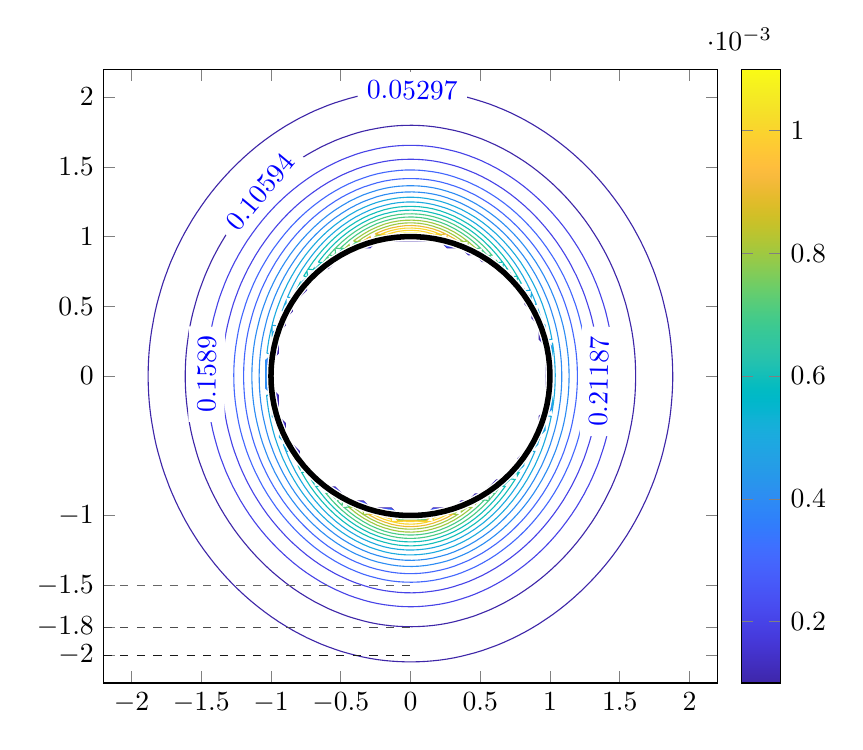
\begin{tikzpicture}

\begin{axis}[%
width=3.069in,
height=3.069in,
at={(0.565in,0.838in)},
scale only axis,
point meta min=0.0001,
point meta max=0.0011,
colormap={mymap}{[1pt] rgb(0pt)=(0.2422,0.1504,0.6603); rgb(1pt)=(0.25039,0.164995,0.707614); rgb(2pt)=(0.257771,0.181781,0.751138); rgb(3pt)=(0.264729,0.197757,0.795214); rgb(4pt)=(0.270648,0.214676,0.836371); rgb(5pt)=(0.275114,0.234238,0.870986); rgb(6pt)=(0.2783,0.255871,0.899071); rgb(7pt)=(0.280333,0.278233,0.9221); rgb(8pt)=(0.281338,0.300595,0.941376); rgb(9pt)=(0.281014,0.322757,0.957886); rgb(10pt)=(0.279467,0.344671,0.971676); rgb(11pt)=(0.275971,0.366681,0.982905); rgb(12pt)=(0.269914,0.3892,0.9906); rgb(13pt)=(0.260243,0.412329,0.995157); rgb(14pt)=(0.244033,0.435833,0.998833); rgb(15pt)=(0.220643,0.460257,0.997286); rgb(16pt)=(0.196333,0.484719,0.989152); rgb(17pt)=(0.183405,0.507371,0.979795); rgb(18pt)=(0.178643,0.528857,0.968157); rgb(19pt)=(0.176438,0.549905,0.952019); rgb(20pt)=(0.168743,0.570262,0.935871); rgb(21pt)=(0.154,0.5902,0.9218); rgb(22pt)=(0.146029,0.609119,0.907857); rgb(23pt)=(0.138024,0.627629,0.89729); rgb(24pt)=(0.124814,0.645929,0.888343); rgb(25pt)=(0.111252,0.6635,0.876314); rgb(26pt)=(0.0952095,0.679829,0.859781); rgb(27pt)=(0.0688714,0.694771,0.839357); rgb(28pt)=(0.0296667,0.708167,0.816333); rgb(29pt)=(0.00357143,0.720267,0.7917); rgb(30pt)=(0.00665714,0.731214,0.766014); rgb(31pt)=(0.0433286,0.741095,0.73941); rgb(32pt)=(0.0963952,0.75,0.712038); rgb(33pt)=(0.140771,0.7584,0.684157); rgb(34pt)=(0.1717,0.766962,0.655443); rgb(35pt)=(0.193767,0.775767,0.6251); rgb(36pt)=(0.216086,0.7843,0.5923); rgb(37pt)=(0.246957,0.791795,0.556743); rgb(38pt)=(0.290614,0.79729,0.518829); rgb(39pt)=(0.340643,0.8008,0.478857); rgb(40pt)=(0.3909,0.802871,0.435448); rgb(41pt)=(0.445629,0.802419,0.390919); rgb(42pt)=(0.5044,0.7993,0.348); rgb(43pt)=(0.561562,0.794233,0.304481); rgb(44pt)=(0.617395,0.787619,0.261238); rgb(45pt)=(0.671986,0.779271,0.2227); rgb(46pt)=(0.7242,0.769843,0.191029); rgb(47pt)=(0.773833,0.759805,0.16461); rgb(48pt)=(0.820314,0.749814,0.153529); rgb(49pt)=(0.863433,0.7406,0.159633); rgb(50pt)=(0.903543,0.733029,0.177414); rgb(51pt)=(0.939257,0.728786,0.209957); rgb(52pt)=(0.972757,0.729771,0.239443); rgb(53pt)=(0.995648,0.743371,0.237148); rgb(54pt)=(0.996986,0.765857,0.219943); rgb(55pt)=(0.995205,0.789252,0.202762); rgb(56pt)=(0.9892,0.813567,0.188533); rgb(57pt)=(0.978629,0.838629,0.176557); rgb(58pt)=(0.967648,0.8639,0.16429); rgb(59pt)=(0.96101,0.889019,0.153676); rgb(60pt)=(0.959671,0.913457,0.142257); rgb(61pt)=(0.962795,0.937338,0.12651); rgb(62pt)=(0.969114,0.960629,0.106362); rgb(63pt)=(0.9769,0.9839,0.0805)},
xmin=-2.2000,
xmax=2.2000,
ymin=-2.2000,
ymax=2.2000,
ytick={-2.0000,-1.8000,-1.5000,-1.0000,0.0000,0.5000,1.0000,1.5000,2.0000},
axis background/.style={fill=white},
colorbar
]
\addplot[contour prepared, contour prepared format=matlab, contour/labels=false] table[row sep=crcr] {%
%
0.0001	315.0000\\
-0.0589	-2.0477\\
-0.0377	-2.0486\\
0.0126	-2.0490\\
0.0628	-2.0478\\
0.0636	-2.0477\\
0.1131	-2.0453\\
0.1633	-2.0412\\
0.2136	-2.0357\\
0.2638	-2.0285\\
0.3141	-2.0196\\
0.3643	-2.0087\\
0.4086	-1.9975\\
0.4146	-1.9961\\
0.4648	-1.9829\\
0.5151	-1.9675\\
0.5653	-1.9497\\
0.5718	-1.9472\\
0.6156	-1.9314\\
0.6658	-1.9106\\
0.6955	-1.8970\\
0.7161	-1.8880\\
0.7663	-1.8638\\
0.7983	-1.8467\\
0.8166	-1.8373\\
0.8668	-1.8091\\
0.8874	-1.7965\\
0.9171	-1.7788\\
0.9663	-1.7462\\
0.9673	-1.7456\\
1.0176	-1.7112\\
1.0380	-1.6960\\
1.0678	-1.6739\\
1.1032	-1.6457\\
1.1181	-1.6337\\
1.1630	-1.5955\\
1.1683	-1.5908\\
1.2183	-1.5452\\
1.2186	-1.5449\\
1.2688	-1.4960\\
1.2698	-1.4950\\
1.3180	-1.4447\\
1.3191	-1.4435\\
1.3631	-1.3945\\
1.3693	-1.3872\\
1.4055	-1.3442\\
1.4196	-1.3264\\
1.4452	-1.2940\\
1.4698	-1.2604\\
1.4822	-1.2437\\
1.5168	-1.1935\\
1.5201	-1.1883\\
1.5500	-1.1432\\
1.5704	-1.1095\\
1.5806	-1.0930\\
1.6096	-1.0427\\
1.6206	-1.0220\\
1.6369	-0.9925\\
1.6621	-0.9422\\
1.6709	-0.9233\\
1.6861	-0.8920\\
1.7083	-0.8417\\
1.7211	-0.8096\\
1.7288	-0.7915\\
1.7484	-0.7412\\
1.7658	-0.6910\\
1.7714	-0.6732\\
1.7824	-0.6407\\
1.7977	-0.5905\\
1.8112	-0.5402\\
1.8216	-0.4960\\
1.8232	-0.4899\\
1.8348	-0.4397\\
1.8449	-0.3894\\
1.8535	-0.3392\\
1.8608	-0.2889\\
1.8667	-0.2387\\
1.8715	-0.1884\\
1.8719	-0.1832\\
1.8755	-0.1382\\
1.8783	-0.0879\\
1.8799	-0.0377\\
1.8802	0.0126\\
1.8792	0.0628\\
1.8771	0.1131\\
1.8736	0.1633\\
1.8719	0.1823\\
1.8693	0.2136\\
1.8639	0.2638\\
1.8573	0.3141\\
1.8494	0.3643\\
1.8401	0.4146\\
1.8292	0.4648\\
1.8216	0.4957\\
1.8173	0.5151\\
1.8047	0.5653\\
1.7903	0.6156\\
1.7740	0.6658\\
1.7714	0.6732\\
1.7574	0.7161\\
1.7389	0.7663\\
1.7211	0.8096\\
1.7184	0.8166\\
1.6975	0.8668\\
1.6740	0.9171\\
1.6709	0.9233\\
1.6499	0.9673\\
1.6230	1.0176\\
1.6206	1.0219\\
1.5956	1.0678\\
1.5704	1.1095\\
1.5653	1.1181\\
1.5338	1.1683\\
1.5201	1.1885\\
1.5000	1.2186\\
1.4698	1.2603\\
1.4637	1.2688\\
1.4253	1.3191\\
1.4196	1.3262\\
1.3848	1.3693\\
1.3693	1.3874\\
1.3413	1.4196\\
1.3191	1.4439\\
1.2948	1.4698\\
1.2688	1.4964\\
1.2450	1.5201\\
1.2186	1.5454\\
1.1915	1.5704\\
1.1683	1.5911\\
1.1338	1.6206\\
1.1181	1.6338\\
1.0711	1.6709\\
1.0678	1.6734\\
1.0176	1.7110\\
1.0031	1.7211\\
0.9673	1.7462\\
0.9280	1.7714\\
0.9171	1.7785\\
0.8668	1.8091\\
0.8443	1.8216\\
0.8166	1.8375\\
0.7663	1.8636\\
0.7490	1.8719\\
0.7161	1.8882\\
0.6658	1.9106\\
0.6370	1.9221\\
0.6156	1.9312\\
0.5653	1.9504\\
0.5151	1.9671\\
0.4972	1.9724\\
0.4648	1.9827\\
0.4146	1.9968\\
0.3643	2.0089\\
0.3141	2.0189\\
0.2924	2.0226\\
0.2638	2.0280\\
0.2136	2.0357\\
0.1633	2.0417\\
0.1131	2.0460\\
0.0628	2.0487\\
0.0126	2.0498\\
-0.0377	2.0494\\
-0.0879	2.0475\\
-0.1382	2.0440\\
-0.1884	2.0389\\
-0.2387	2.0321\\
-0.2889	2.0234\\
-0.2930	2.0226\\
-0.3392	2.0141\\
-0.3894	2.0031\\
-0.4397	1.9901\\
-0.4899	1.9748\\
-0.4973	1.9724\\
-0.5402	1.9590\\
-0.5905	1.9411\\
-0.6370	1.9221\\
-0.6407	1.9207\\
-0.6910	1.8998\\
-0.7412	1.8758\\
-0.7489	1.8719\\
-0.7915	1.8510\\
-0.8417	1.8231\\
-0.8442	1.8216\\
-0.8920	1.7943\\
-0.9281	1.7714\\
-0.9422	1.7625\\
-0.9925	1.7287\\
-1.0031	1.7211\\
-1.0427	1.6929\\
-1.0713	1.6709\\
-1.0930	1.6542\\
-1.1337	1.6206\\
-1.1432	1.6126\\
-1.1911	1.5704\\
-1.1935	1.5682\\
-1.2437	1.5209\\
-1.2445	1.5201\\
-1.2940	1.4702\\
-1.2943	1.4698\\
-1.3409	1.4196\\
-1.3442	1.4158\\
-1.3847	1.3693\\
-1.3945	1.3574\\
-1.4257	1.3191\\
-1.4447	1.2941\\
-1.4640	1.2688\\
-1.4950	1.2251\\
-1.4996	1.2186\\
-1.5337	1.1683\\
-1.5452	1.1500\\
-1.5657	1.1181\\
-1.5949	1.0678\\
-1.5955	1.0668\\
-1.6236	1.0176\\
-1.6457	0.9742\\
-1.6494	0.9673\\
-1.6745	0.9171\\
-1.6960	0.8687\\
-1.6968	0.8668\\
-1.7190	0.8166\\
-1.7386	0.7663\\
-1.7462	0.7449\\
-1.7572	0.7161\\
-1.7746	0.6658\\
-1.7899	0.6156\\
-1.7965	0.5917\\
-1.8043	0.5653\\
-1.8178	0.5151\\
-1.8295	0.4648\\
-1.8397	0.4146\\
-1.8467	0.3745\\
-1.8487	0.3643\\
-1.8572	0.3141\\
-1.8642	0.2638\\
-1.8699	0.2136\\
-1.8744	0.1633\\
-1.8776	0.1131\\
-1.8796	0.0628\\
-1.8805	0.0126\\
-1.8802	-0.0377\\
-1.8787	-0.0879\\
-1.8761	-0.1382\\
-1.8723	-0.1884\\
-1.8672	-0.2387\\
-1.8609	-0.2889\\
-1.8531	-0.3392\\
-1.8467	-0.3744\\
-1.8443	-0.3894\\
-1.8348	-0.4397\\
-1.8239	-0.4899\\
-1.8113	-0.5402\\
-1.7969	-0.5905\\
-1.7965	-0.5919\\
-1.7825	-0.6407\\
-1.7662	-0.6910\\
-1.7477	-0.7412\\
-1.7462	-0.7450\\
-1.7291	-0.7915\\
-1.7083	-0.8417\\
-1.6960	-0.8687\\
-1.6860	-0.8920\\
-1.6623	-0.9422\\
-1.6457	-0.9742\\
-1.6367	-0.9925\\
-1.6097	-1.0427\\
-1.5955	-1.0670\\
-1.5808	-1.0930\\
-1.5496	-1.1432\\
-1.5452	-1.1499\\
-1.5172	-1.1935\\
-1.4950	-1.2252\\
-1.4822	-1.2437\\
-1.4447	-1.2938\\
-1.4446	-1.2940\\
-1.4054	-1.3442\\
-1.3945	-1.3574\\
-1.3634	-1.3945\\
-1.3442	-1.4161\\
-1.3184	-1.4447\\
-1.2940	-1.4706\\
-1.2703	-1.4950\\
-1.2437	-1.5214\\
-1.2187	-1.5452\\
-1.1935	-1.5687\\
-1.1632	-1.5955\\
-1.1432	-1.6128\\
-1.1031	-1.6457\\
-1.0930	-1.6540\\
-1.0427	-1.6924\\
-1.0378	-1.6960\\
-0.9925	-1.7290\\
-0.9666	-1.7462\\
-0.9422	-1.7627\\
-0.8920	-1.7938\\
-0.8873	-1.7965\\
-0.8417	-1.8237\\
-0.7983	-1.8467\\
-0.7915	-1.8505\\
-0.7412	-1.8763\\
-0.6955	-1.8970\\
-0.6910	-1.8992\\
-0.6407	-1.9214\\
-0.5905	-1.9407\\
-0.5717	-1.9472\\
-0.5402	-1.9590\\
-0.4899	-1.9755\\
-0.4397	-1.9898\\
-0.4083	-1.9975\\
-0.3894	-2.0026\\
-0.3392	-2.0144\\
-0.2889	-2.0242\\
-0.2387	-2.0323\\
-0.1884	-2.0387\\
-0.1382	-2.0434\\
-0.0879	-2.0467\\
-0.0589	-2.0477\\
0.0001	161.0000\\
0.1155	-0.9925\\
0.1131	-0.9952\\
0.0628	-0.9951\\
0.0126	-0.9951\\
-0.0377	-0.9951\\
-0.0879	-0.9952\\
-0.0903	-0.9925\\
-0.1382	-0.9446\\
-0.1884	-0.9447\\
-0.2387	-0.9449\\
-0.2889	-0.9451\\
-0.2917	-0.9422\\
-0.3392	-0.8947\\
-0.3894	-0.8950\\
-0.4397	-0.8953\\
-0.4430	-0.8920\\
-0.4899	-0.8450\\
-0.4933	-0.8417\\
-0.5402	-0.7948\\
-0.5905	-0.7952\\
-0.5943	-0.7915\\
-0.6407	-0.7451\\
-0.6447	-0.7412\\
-0.6910	-0.6949\\
-0.6951	-0.6910\\
-0.7412	-0.6449\\
-0.7456	-0.6407\\
-0.7915	-0.5949\\
-0.7962	-0.5905\\
-0.7959	-0.5402\\
-0.8417	-0.4944\\
-0.8465	-0.4899\\
-0.8920	-0.4445\\
-0.8972	-0.4397\\
-0.8970	-0.3894\\
-0.8968	-0.3392\\
-0.9422	-0.2938\\
-0.9476	-0.2889\\
-0.9475	-0.2387\\
-0.9474	-0.1884\\
-0.9473	-0.1382\\
-0.9925	-0.0930\\
-0.9982	-0.0879\\
-0.9981	-0.0377\\
-0.9981	0.0126\\
-0.9981	0.0628\\
-0.9982	0.1131\\
-0.9925	0.1182\\
-0.9473	0.1633\\
-0.9474	0.2136\\
-0.9475	0.2638\\
-0.9476	0.3141\\
-0.9422	0.3190\\
-0.8969	0.3643\\
-0.8971	0.4146\\
-0.8920	0.4193\\
-0.8464	0.4648\\
-0.8466	0.5151\\
-0.8417	0.5197\\
-0.7960	0.5653\\
-0.7915	0.5696\\
-0.7455	0.6156\\
-0.7458	0.6658\\
-0.7412	0.6702\\
-0.6953	0.7161\\
-0.6910	0.7202\\
-0.6448	0.7663\\
-0.6407	0.7703\\
-0.5905	0.7699\\
-0.5438	0.8166\\
-0.5402	0.8201\\
-0.4935	0.8668\\
-0.4899	0.8703\\
-0.4397	0.8700\\
-0.3926	0.9171\\
-0.3894	0.9203\\
-0.3392	0.9200\\
-0.2889	0.9198\\
-0.2414	0.9673\\
-0.2387	0.9702\\
-0.1884	0.9701\\
-0.1382	0.9699\\
-0.0879	0.9698\\
-0.0377	0.9698\\
0.0126	0.9698\\
0.0628	0.9698\\
0.1131	0.9699\\
0.1633	0.9700\\
0.2136	0.9701\\
0.2162	0.9673\\
0.2638	0.9197\\
0.3141	0.9199\\
0.3643	0.9202\\
0.3673	0.9171\\
0.4146	0.8699\\
0.4648	0.8702\\
0.4682	0.8668\\
0.5151	0.8199\\
0.5653	0.8203\\
0.5691	0.8166\\
0.6156	0.7701\\
0.6195	0.7663\\
0.6658	0.7200\\
0.6699	0.7161\\
0.7161	0.6699\\
0.7204	0.6658\\
0.7663	0.6199\\
0.7709	0.6156\\
0.8166	0.5699\\
0.8214	0.5653\\
0.8212	0.5151\\
0.8668	0.4695\\
0.8718	0.4648\\
0.8716	0.4146\\
0.9171	0.3691\\
0.9223	0.3643\\
0.9222	0.3141\\
0.9221	0.2638\\
0.9673	0.2186\\
0.9729	0.2136\\
0.9728	0.1633\\
0.9727	0.1131\\
0.9727	0.0628\\
0.9727	0.0126\\
0.9727	-0.0377\\
0.9727	-0.0879\\
0.9727	-0.1382\\
0.9728	-0.1884\\
0.9729	-0.2387\\
0.9673	-0.2437\\
0.9221	-0.2889\\
0.9223	-0.3392\\
0.9224	-0.3894\\
0.9171	-0.3944\\
0.8717	-0.4397\\
0.8719	-0.4899\\
0.8668	-0.4947\\
0.8213	-0.5402\\
0.8166	-0.5446\\
0.7708	-0.5905\\
0.7710	-0.6407\\
0.7663	-0.6451\\
0.7205	-0.6910\\
0.7161	-0.6952\\
0.6701	-0.7412\\
0.6658	-0.7453\\
0.6156	-0.7448\\
0.5690	-0.7915\\
0.5653	-0.7950\\
0.5186	-0.8417\\
0.5151	-0.8452\\
0.4648	-0.8449\\
0.4177	-0.8920\\
0.4146	-0.8952\\
0.3643	-0.8949\\
0.3170	-0.9422\\
0.3141	-0.9452\\
0.2638	-0.9450\\
0.2136	-0.9448\\
0.1633	-0.9447\\
0.1155	-0.9925\\
0.0001	273.0000\\
-0.0154	-1.7965\\
0.0126	-1.7968\\
0.0219	-1.7965\\
0.0628	-1.7954\\
0.1131	-1.7924\\
0.1633	-1.7875\\
0.2136	-1.7808\\
0.2638	-1.7720\\
0.3141	-1.7611\\
0.3643	-1.7477\\
0.3692	-1.7462\\
0.4146	-1.7336\\
0.4648	-1.7170\\
0.5151	-1.6975\\
0.5187	-1.6960\\
0.5653	-1.6773\\
0.6156	-1.6540\\
0.6317	-1.6457\\
0.6658	-1.6289\\
0.7161	-1.6009\\
0.7252	-1.5955\\
0.7663	-1.5713\\
0.8060	-1.5452\\
0.8166	-1.5383\\
0.8668	-1.5031\\
0.8776	-1.4950\\
0.9171	-1.4651\\
0.9422	-1.4447\\
0.9673	-1.4239\\
1.0007	-1.3945\\
1.0176	-1.3792\\
1.0544	-1.3442\\
1.0678	-1.3309\\
1.1039	-1.2940\\
1.1181	-1.2787\\
1.1498	-1.2437\\
1.1683	-1.2220\\
1.1924	-1.1935\\
1.2186	-1.1600\\
1.2318	-1.1432\\
1.2681	-1.0930\\
1.2688	-1.0919\\
1.3030	-1.0427\\
1.3191	-1.0171\\
1.3349	-0.9925\\
1.3644	-0.9422\\
1.3693	-0.9330\\
1.3925	-0.8920\\
1.4177	-0.8417\\
1.4196	-0.8376\\
1.4422	-0.7915\\
1.4639	-0.7412\\
1.4698	-0.7262\\
1.4847	-0.6910\\
1.5035	-0.6407\\
1.5200	-0.5905\\
1.5201	-0.5901\\
1.5363	-0.5402\\
1.5505	-0.4899\\
1.5628	-0.4397\\
1.5704	-0.4043\\
1.5738	-0.3894\\
1.5841	-0.3392\\
1.5926	-0.2889\\
1.5997	-0.2387\\
1.6053	-0.1884\\
1.6095	-0.1382\\
1.6123	-0.0879\\
1.6139	-0.0377\\
1.6142	0.0126\\
1.6133	0.0628\\
1.6111	0.1131\\
1.6075	0.1633\\
1.6026	0.2136\\
1.5963	0.2638\\
1.5886	0.3141\\
1.5792	0.3643\\
1.5704	0.4044\\
1.5683	0.4146\\
1.5569	0.4648\\
1.5437	0.5151\\
1.5284	0.5653\\
1.5201	0.5899\\
1.5120	0.6156\\
1.4944	0.6658\\
1.4743	0.7161\\
1.4698	0.7263\\
1.4534	0.7663\\
1.4302	0.8166\\
1.4196	0.8377\\
1.4055	0.8668\\
1.3786	0.9171\\
1.3693	0.9331\\
1.3501	0.9673\\
1.3191	1.0169\\
1.3186	1.0176\\
1.2861	1.0678\\
1.2688	1.0922\\
1.2506	1.1181\\
1.2186	1.1599\\
1.2122	1.1683\\
1.1710	1.2186\\
1.1683	1.2217\\
1.1271	1.2688\\
1.1181	1.2786\\
1.0796	1.3191\\
1.0678	1.3309\\
1.0280	1.3693\\
1.0176	1.3791\\
0.9718	1.4196\\
0.9673	1.4235\\
0.9171	1.4648\\
0.9105	1.4698\\
0.8668	1.5033\\
0.8429	1.5201\\
0.8166	1.5386\\
0.7668	1.5704\\
0.7663	1.5706\\
0.7161	1.6013\\
0.6803	1.6206\\
0.6658	1.6287\\
0.6156	1.6542\\
0.5783	1.6709\\
0.5653	1.6769\\
0.5151	1.6983\\
0.4648	1.7165\\
0.4504	1.7211\\
0.4146	1.7335\\
0.3643	1.7485\\
0.3141	1.7609\\
0.2638	1.7711\\
0.2625	1.7714\\
0.2136	1.7805\\
0.1633	1.7878\\
0.1131	1.7930\\
0.0628	1.7963\\
0.0126	1.7977\\
-0.0377	1.7972\\
-0.0879	1.7949\\
-0.1382	1.7906\\
-0.1884	1.7844\\
-0.2387	1.7761\\
-0.2617	1.7714\\
-0.2889	1.7663\\
-0.3392	1.7550\\
-0.3894	1.7413\\
-0.4397	1.7250\\
-0.4505	1.7211\\
-0.4899	1.7077\\
-0.5402	1.6880\\
-0.5782	1.6709\\
-0.5905	1.6656\\
-0.6407	1.6419\\
-0.6803	1.6206\\
-0.6910	1.6151\\
-0.7412	1.5866\\
-0.7670	1.5704\\
-0.7915	1.5552\\
-0.8417	1.5208\\
-0.8426	1.5201\\
-0.8920	1.4845\\
-0.9107	1.4698\\
-0.9422	1.4449\\
-0.9721	1.4196\\
-0.9925	1.4020\\
-1.0281	1.3693\\
-1.0427	1.3556\\
-1.0796	1.3191\\
-1.0930	1.3054\\
-1.1273	1.2688\\
-1.1432	1.2510\\
-1.1715	1.2186\\
-1.1935	1.1917\\
-1.2124	1.1683\\
-1.2437	1.1268\\
-1.2503	1.1181\\
-1.2859	1.0678\\
-1.2940	1.0555\\
-1.3193	1.0176\\
-1.3442	0.9763\\
-1.3497	0.9673\\
-1.3788	0.9171\\
-1.3945	0.8870\\
-1.4054	0.8668\\
-1.4304	0.8166\\
-1.4447	0.7844\\
-1.4532	0.7663\\
-1.4748	0.7161\\
-1.4937	0.6658\\
-1.4950	0.6622\\
-1.5123	0.6156\\
-1.5287	0.5653\\
-1.5430	0.5151\\
-1.5452	0.5064\\
-1.5568	0.4648\\
-1.5690	0.4146\\
-1.5794	0.3643\\
-1.5882	0.3141\\
-1.5955	0.2641\\
-1.5955	0.2638\\
-1.6022	0.2136\\
-1.6075	0.1633\\
-1.6112	0.1131\\
-1.6136	0.0628\\
-1.6146	0.0126\\
-1.6143	-0.0377\\
-1.6126	-0.0879\\
-1.6095	-0.1382\\
-1.6050	-0.1884\\
-1.5991	-0.2387\\
-1.5955	-0.2630\\
-1.5920	-0.2889\\
-1.5840	-0.3392\\
-1.5744	-0.3894\\
-1.5631	-0.4397\\
-1.5500	-0.4899\\
-1.5452	-0.5063\\
-1.5361	-0.5402\\
-1.5208	-0.5905\\
-1.5032	-0.6407\\
-1.4950	-0.6621\\
-1.4846	-0.6910\\
-1.4643	-0.7412\\
-1.4447	-0.7843\\
-1.4417	-0.7915\\
-1.4183	-0.8417\\
-1.3945	-0.8870\\
-1.3920	-0.8920\\
-1.3648	-0.9422\\
-1.3442	-0.9763\\
-1.3348	-0.9925\\
-1.3027	-1.0427\\
-1.2940	-1.0555\\
-1.2687	-1.0930\\
-1.2437	-1.1269\\
-1.2317	-1.1432\\
-1.1935	-1.1914\\
-1.1918	-1.1935\\
-1.1495	-1.2437\\
-1.1432	-1.2508\\
-1.1038	-1.2940\\
-1.0930	-1.3053\\
-1.0544	-1.3442\\
-1.0427	-1.3555\\
-1.0006	-1.3945\\
-0.9925	-1.4018\\
-0.9422	-1.4444\\
-0.9418	-1.4447\\
-0.8920	-1.4844\\
-0.8777	-1.4950\\
-0.8417	-1.5214\\
-0.8061	-1.5452\\
-0.7915	-1.5551\\
-0.7412	-1.5864\\
-0.7252	-1.5955\\
-0.6910	-1.6155\\
-0.6407	-1.6414\\
-0.6316	-1.6457\\
-0.5905	-1.6661\\
-0.5402	-1.6877\\
-0.5186	-1.6960\\
-0.4899	-1.7077\\
-0.4397	-1.7256\\
-0.3894	-1.7408\\
-0.3688	-1.7462\\
-0.3392	-1.7547\\
-0.2889	-1.7668\\
-0.2387	-1.7767\\
-0.1884	-1.7844\\
-0.1382	-1.7902\\
-0.0879	-1.7941\\
-0.0377	-1.7963\\
-0.0154	-1.7965\\
0.0001	161.0000\\
0.1180	-0.9925\\
0.1131	-0.9979\\
0.0628	-0.9978\\
0.0126	-0.9977\\
-0.0377	-0.9978\\
-0.0879	-0.9979\\
-0.0927	-0.9925\\
-0.1382	-0.9470\\
-0.1884	-0.9473\\
-0.2387	-0.9476\\
-0.2889	-0.9480\\
-0.2945	-0.9422\\
-0.3392	-0.8975\\
-0.3894	-0.8980\\
-0.4397	-0.8987\\
-0.4464	-0.8920\\
-0.4899	-0.8484\\
-0.4967	-0.8417\\
-0.5402	-0.7982\\
-0.5905	-0.7990\\
-0.5982	-0.7915\\
-0.6407	-0.7489\\
-0.6487	-0.7412\\
-0.6910	-0.6989\\
-0.6993	-0.6910\\
-0.7412	-0.6491\\
-0.7500	-0.6407\\
-0.7915	-0.5993\\
-0.8009	-0.5905\\
-0.8004	-0.5402\\
-0.8417	-0.4989\\
-0.8513	-0.4899\\
-0.8920	-0.4493\\
-0.9024	-0.4397\\
-0.9020	-0.3894\\
-0.9017	-0.3392\\
-0.9422	-0.2987\\
-0.9529	-0.2889\\
-0.9527	-0.2387\\
-0.9525	-0.1884\\
-0.9524	-0.1382\\
-0.9925	-0.0981\\
-1.0039	-0.0879\\
-1.0038	-0.0377\\
-1.0038	0.0126\\
-1.0038	0.0628\\
-1.0039	0.1131\\
-0.9925	0.1233\\
-0.9524	0.1633\\
-0.9526	0.2136\\
-0.9528	0.2638\\
-0.9531	0.3141\\
-0.9422	0.3240\\
-0.9019	0.3643\\
-0.9022	0.4146\\
-0.8920	0.4240\\
-0.8511	0.4648\\
-0.8515	0.5151\\
-0.8417	0.5242\\
-0.8006	0.5653\\
-0.7915	0.5739\\
-0.7498	0.6156\\
-0.7503	0.6658\\
-0.7412	0.6745\\
-0.6996	0.7161\\
-0.6910	0.7244\\
-0.6490	0.7663\\
-0.6407	0.7744\\
-0.5905	0.7735\\
-0.5474	0.8166\\
-0.5402	0.8236\\
-0.4970	0.8668\\
-0.4899	0.8739\\
-0.4397	0.8732\\
-0.3958	0.9171\\
-0.3894	0.9235\\
-0.3392	0.9230\\
-0.2889	0.9225\\
-0.2441	0.9673\\
-0.2387	0.9731\\
-0.1884	0.9728\\
-0.1382	0.9725\\
-0.0879	0.9723\\
-0.0377	0.9722\\
0.0126	0.9722\\
0.0628	0.9723\\
0.1131	0.9724\\
0.1633	0.9726\\
0.2136	0.9729\\
0.2188	0.9673\\
0.2638	0.9223\\
0.3141	0.9227\\
0.3643	0.9233\\
0.3704	0.9171\\
0.4146	0.8729\\
0.4648	0.8735\\
0.4715	0.8668\\
0.5151	0.8233\\
0.5653	0.8240\\
0.5729	0.8166\\
0.6156	0.7739\\
0.6234	0.7663\\
0.6658	0.7239\\
0.6740	0.7161\\
0.7161	0.6740\\
0.7247	0.6658\\
0.7663	0.6242\\
0.7754	0.6156\\
0.8166	0.5744\\
0.8263	0.5653\\
0.8258	0.5151\\
0.8668	0.4741\\
0.8768	0.4648\\
0.8765	0.4146\\
0.9171	0.3740\\
0.9276	0.3643\\
0.9273	0.3141\\
0.9271	0.2638\\
0.9673	0.2235\\
0.9784	0.2136\\
0.9782	0.1633\\
0.9781	0.1131\\
0.9780	0.0628\\
0.9780	0.0126\\
0.9780	-0.0377\\
0.9780	-0.0879\\
0.9781	-0.1382\\
0.9783	-0.1884\\
0.9785	-0.2387\\
0.9673	-0.2488\\
0.9272	-0.2889\\
0.9274	-0.3392\\
0.9278	-0.3894\\
0.9171	-0.3993\\
0.8766	-0.4397\\
0.8770	-0.4899\\
0.8668	-0.4994\\
0.8261	-0.5402\\
0.8166	-0.5491\\
0.7752	-0.5905\\
0.7757	-0.6407\\
0.7663	-0.6496\\
0.7249	-0.6910\\
0.7161	-0.6994\\
0.6743	-0.7412\\
0.6658	-0.7494\\
0.6156	-0.7485\\
0.5726	-0.7915\\
0.5653	-0.7986\\
0.5222	-0.8417\\
0.5151	-0.8487\\
0.4648	-0.8480\\
0.4209	-0.8920\\
0.4146	-0.8983\\
0.3643	-0.8978\\
0.3199	-0.9422\\
0.3141	-0.9483\\
0.2638	-0.9478\\
0.2136	-0.9474\\
0.1633	-0.9471\\
0.1180	-0.9925\\
0.0002	249.0000\\
-0.1340	-1.6457\\
-0.0879	-1.6504\\
-0.0377	-1.6531\\
0.0126	-1.6537\\
0.0628	-1.6520\\
0.1131	-1.6481\\
0.1326	-1.6457\\
0.1633	-1.6424\\
0.2136	-1.6349\\
0.2638	-1.6251\\
0.3141	-1.6127\\
0.3643	-1.5976\\
0.3705	-1.5955\\
0.4146	-1.5814\\
0.4648	-1.5624\\
0.5039	-1.5452\\
0.5151	-1.5406\\
0.5653	-1.5172\\
0.6066	-1.4950\\
0.6156	-1.4903\\
0.6658	-1.4616\\
0.6922	-1.4447\\
0.7161	-1.4297\\
0.7661	-1.3945\\
0.7663	-1.3943\\
0.8166	-1.3568\\
0.8321	-1.3442\\
0.8668	-1.3155\\
0.8913	-1.2940\\
0.9171	-1.2705\\
0.9450	-1.2437\\
0.9673	-1.2213\\
0.9942	-1.1935\\
1.0176	-1.1677\\
1.0393	-1.1432\\
1.0678	-1.1089\\
1.0809	-1.0930\\
1.1181	-1.0439\\
1.1190	-1.0427\\
1.1551	-0.9925\\
1.1683	-0.9722\\
1.1883	-0.9422\\
1.2183	-0.8920\\
1.2186	-0.8914\\
1.2473	-0.8417\\
1.2688	-0.7994\\
1.2730	-0.7915\\
1.2978	-0.7412\\
1.3191	-0.6914\\
1.3193	-0.6910\\
1.3405	-0.6407\\
1.3589	-0.5905\\
1.3693	-0.5583\\
1.3757	-0.5402\\
1.3914	-0.4899\\
1.4050	-0.4397\\
1.4166	-0.3894\\
1.4196	-0.3745\\
1.4274	-0.3392\\
1.4368	-0.2889\\
1.4444	-0.2387\\
1.4505	-0.1884\\
1.4551	-0.1382\\
1.4582	-0.0879\\
1.4599	-0.0377\\
1.4603	0.0126\\
1.4592	0.0628\\
1.4568	0.1131\\
1.4530	0.1633\\
1.4477	0.2136\\
1.4408	0.2638\\
1.4323	0.3141\\
1.4220	0.3643\\
1.4196	0.3746\\
1.4110	0.4146\\
1.3985	0.4648\\
1.3838	0.5151\\
1.3693	0.5584\\
1.3672	0.5653\\
1.3500	0.6156\\
1.3303	0.6658\\
1.3191	0.6914\\
1.3089	0.7161\\
1.2858	0.7663\\
1.2688	0.7994\\
1.2604	0.8166\\
1.2333	0.8668\\
1.2186	0.8915\\
1.2038	0.9171\\
1.1716	0.9673\\
1.1683	0.9721\\
1.1377	1.0176\\
1.1181	1.0441\\
1.1006	1.0678\\
1.0678	1.1088\\
1.0603	1.1181\\
1.0176	1.1673\\
1.0167	1.1683\\
0.9697	1.2186\\
0.9673	1.2210\\
0.9183	1.2688\\
0.9171	1.2700\\
0.8668	1.3151\\
0.8622	1.3191\\
0.8166	1.3568\\
0.8001	1.3693\\
0.7663	1.3949\\
0.7305	1.4196\\
0.7161	1.4295\\
0.6658	1.4614\\
0.6511	1.4698\\
0.6156	1.4907\\
0.5653	1.5166\\
0.5579	1.5201\\
0.5151	1.5411\\
0.4648	1.5622\\
0.4425	1.5704\\
0.4146	1.5813\\
0.3643	1.5983\\
0.3141	1.6124\\
0.2788	1.6206\\
0.2638	1.6244\\
0.2136	1.6350\\
0.1633	1.6431\\
0.1131	1.6489\\
0.0628	1.6525\\
0.0126	1.6541\\
-0.0377	1.6536\\
-0.0879	1.6510\\
-0.1382	1.6463\\
-0.1884	1.6393\\
-0.2387	1.6300\\
-0.2789	1.6206\\
-0.2889	1.6185\\
-0.3392	1.6057\\
-0.3894	1.5902\\
-0.4397	1.5716\\
-0.4427	1.5704\\
-0.4899	1.5521\\
-0.5402	1.5291\\
-0.5580	1.5201\\
-0.5905	1.5042\\
-0.6407	1.4761\\
-0.6511	1.4698\\
-0.6910	1.4461\\
-0.7304	1.4196\\
-0.7412	1.4124\\
-0.7915	1.3760\\
-0.8000	1.3693\\
-0.8417	1.3366\\
-0.8624	1.3191\\
-0.8920	1.2935\\
-0.9188	1.2688\\
-0.9422	1.2464\\
-0.9701	1.2186\\
-0.9925	1.1951\\
-1.0172	1.1683\\
-1.0427	1.1390\\
-1.0605	1.1181\\
-1.0930	1.0772\\
-1.1003	1.0678\\
-1.1374	1.0176\\
-1.1432	1.0090\\
-1.1721	0.9673\\
-1.1935	0.9331\\
-1.2037	0.9171\\
-1.2332	0.8668\\
-1.2437	0.8471\\
-1.2606	0.8166\\
-1.2856	0.7663\\
-1.2940	0.7478\\
-1.3090	0.7161\\
-1.3304	0.6658\\
-1.3442	0.6289\\
-1.3496	0.6156\\
-1.3679	0.5653\\
-1.3837	0.5151\\
-1.3945	0.4761\\
-1.3979	0.4648\\
-1.4113	0.4146\\
-1.4227	0.3643\\
-1.4323	0.3141\\
-1.4403	0.2638\\
-1.4447	0.2294\\
-1.4470	0.2136\\
-1.4527	0.1633\\
-1.4568	0.1131\\
-1.4593	0.0628\\
-1.4604	0.0126\\
-1.4601	-0.0377\\
-1.4582	-0.0879\\
-1.4549	-0.1382\\
-1.4500	-0.1884\\
-1.4447	-0.2297\\
-1.4437	-0.2387\\
-1.4365	-0.2889\\
-1.4277	-0.3392\\
-1.4172	-0.3894\\
-1.4048	-0.4397\\
-1.3945	-0.4761\\
-1.3908	-0.4899\\
-1.3761	-0.5402\\
-1.3590	-0.5905\\
-1.3442	-0.6289\\
-1.3400	-0.6407\\
-1.3201	-0.6910\\
-1.2972	-0.7412\\
-1.2940	-0.7478\\
-1.2735	-0.7915\\
-1.2468	-0.8417\\
-1.2437	-0.8471\\
-1.2190	-0.8920\\
-1.1935	-0.9330\\
-1.1879	-0.9422\\
-1.1551	-0.9925\\
-1.1432	-1.0091\\
-1.1196	-1.0427\\
-1.0930	-1.0773\\
-1.0809	-1.0930\\
-1.0427	-1.1387\\
-1.0389	-1.1432\\
-0.9937	-1.1935\\
-0.9925	-1.1947\\
-0.9446	-1.2437\\
-0.9422	-1.2460\\
-0.8920	-1.2930\\
-0.8909	-1.2940\\
-0.8417	-1.3364\\
-0.8320	-1.3442\\
-0.7915	-1.3763\\
-0.7664	-1.3945\\
-0.7412	-1.4127\\
-0.6920	-1.4447\\
-0.6910	-1.4454\\
-0.6407	-1.4765\\
-0.6066	-1.4950\\
-0.5905	-1.5040\\
-0.5402	-1.5294\\
-0.5039	-1.5452\\
-0.4899	-1.5517\\
-0.4397	-1.5724\\
-0.3894	-1.5898\\
-0.3703	-1.5955\\
-0.3392	-1.6055\\
-0.2889	-1.6192\\
-0.2387	-1.6303\\
-0.1884	-1.6389\\
-0.1382	-1.6454\\
-0.1340	-1.6457\\
0.0002	161.0000\\
0.1204	-0.9925\\
0.1131	-1.0007\\
0.0628	-1.0005\\
0.0126	-1.0004\\
-0.0377	-1.0004\\
-0.0879	-1.0006\\
-0.0951	-0.9925\\
-0.1382	-0.9494\\
-0.1884	-0.9498\\
-0.2387	-0.9503\\
-0.2889	-0.9509\\
-0.2973	-0.9422\\
-0.3392	-0.9003\\
-0.3894	-0.9011\\
-0.4397	-0.9020\\
-0.4497	-0.8920\\
-0.4899	-0.8517\\
-0.5000	-0.8417\\
-0.5402	-0.8015\\
-0.5905	-0.8027\\
-0.6020	-0.7915\\
-0.6407	-0.7528\\
-0.6527	-0.7412\\
-0.6910	-0.7029\\
-0.7035	-0.6910\\
-0.7412	-0.6533\\
-0.7545	-0.6407\\
-0.7915	-0.6037\\
-0.8055	-0.5905\\
-0.8049	-0.5402\\
-0.8417	-0.5033\\
-0.8561	-0.4899\\
-0.8920	-0.4541\\
-0.9076	-0.4397\\
-0.9070	-0.3894\\
-0.9066	-0.3392\\
-0.9422	-0.3036\\
-0.9583	-0.2889\\
-0.9579	-0.2387\\
-0.9577	-0.1884\\
-0.9575	-0.1382\\
-0.9925	-0.1032\\
-1.0096	-0.0879\\
-1.0095	-0.0377\\
-1.0094	0.0126\\
-1.0095	0.0628\\
-1.0096	0.1131\\
-0.9925	0.1284\\
-0.9576	0.1633\\
-0.9578	0.2136\\
-0.9581	0.2638\\
-0.9585	0.3141\\
-0.9422	0.3289\\
-0.9068	0.3643\\
-0.9073	0.4146\\
-0.8920	0.4287\\
-0.8558	0.4648\\
-0.8565	0.5151\\
-0.8417	0.5288\\
-0.8052	0.5653\\
-0.7915	0.5782\\
-0.7541	0.6156\\
-0.7549	0.6658\\
-0.7412	0.6788\\
-0.7039	0.7161\\
-0.6910	0.7285\\
-0.6531	0.7663\\
-0.6407	0.7784\\
-0.5905	0.7771\\
-0.5510	0.8166\\
-0.5402	0.8272\\
-0.5005	0.8668\\
-0.4899	0.8774\\
-0.4397	0.8763\\
-0.3990	0.9171\\
-0.3894	0.9268\\
-0.3392	0.9259\\
-0.2889	0.9252\\
-0.2468	0.9673\\
-0.2387	0.9760\\
-0.1884	0.9755\\
-0.1382	0.9751\\
-0.0879	0.9748\\
-0.0377	0.9747\\
0.0126	0.9746\\
0.0628	0.9747\\
0.1131	0.9749\\
0.1633	0.9753\\
0.2136	0.9757\\
0.2214	0.9673\\
0.2638	0.9249\\
0.3141	0.9256\\
0.3643	0.9264\\
0.3734	0.9171\\
0.4146	0.8759\\
0.4648	0.8768\\
0.4748	0.8668\\
0.5151	0.8266\\
0.5653	0.8277\\
0.5767	0.8166\\
0.6156	0.7777\\
0.6273	0.7663\\
0.6658	0.7278\\
0.6781	0.7161\\
0.7161	0.6781\\
0.7290	0.6658\\
0.7663	0.6285\\
0.7800	0.6156\\
0.8166	0.5790\\
0.8312	0.5653\\
0.8305	0.5151\\
0.8668	0.4787\\
0.8818	0.4648\\
0.8813	0.4146\\
0.9171	0.3788\\
0.9329	0.3643\\
0.9324	0.3141\\
0.9320	0.2638\\
0.9673	0.2285\\
0.9839	0.2136\\
0.9837	0.1633\\
0.9835	0.1131\\
0.9833	0.0628\\
0.9833	0.0126\\
0.9833	-0.0377\\
0.9834	-0.0879\\
0.9835	-0.1382\\
0.9838	-0.1884\\
0.9841	-0.2387\\
0.9673	-0.2538\\
0.9322	-0.2889\\
0.9326	-0.3392\\
0.9331	-0.3894\\
0.9171	-0.4042\\
0.8815	-0.4397\\
0.8822	-0.4899\\
0.8668	-0.5042\\
0.8308	-0.5402\\
0.8166	-0.5535\\
0.7796	-0.5905\\
0.7804	-0.6407\\
0.7663	-0.6540\\
0.7294	-0.6910\\
0.7161	-0.7036\\
0.6785	-0.7412\\
0.6658	-0.7534\\
0.6156	-0.7521\\
0.5762	-0.7915\\
0.5653	-0.8021\\
0.5257	-0.8417\\
0.5151	-0.8522\\
0.4648	-0.8512\\
0.4241	-0.8920\\
0.4146	-0.9015\\
0.3643	-0.9007\\
0.3228	-0.9422\\
0.3141	-0.9513\\
0.2638	-0.9506\\
0.2136	-0.9500\\
0.1633	-0.9496\\
0.1204	-0.9925\\
0.0002	233.0000\\
-0.1326	-1.5452\\
-0.0879	-1.5502\\
-0.0377	-1.5533\\
0.0126	-1.5539\\
0.0628	-1.5520\\
0.1131	-1.5477\\
0.1315	-1.5452\\
0.1633	-1.5414\\
0.2136	-1.5331\\
0.2638	-1.5222\\
0.3141	-1.5084\\
0.3545	-1.4950\\
0.3643	-1.4920\\
0.4146	-1.4741\\
0.4648	-1.4525\\
0.4810	-1.4447\\
0.5151	-1.4290\\
0.5653	-1.4021\\
0.5783	-1.3945\\
0.6156	-1.3730\\
0.6593	-1.3442\\
0.6658	-1.3399\\
0.7161	-1.3043\\
0.7295	-1.2940\\
0.7663	-1.2652\\
0.7917	-1.2437\\
0.8166	-1.2221\\
0.8475	-1.1935\\
0.8668	-1.1748\\
0.8981	-1.1432\\
0.9171	-1.1229\\
0.9442	-1.0930\\
0.9673	-1.0657\\
0.9865	-1.0427\\
1.0176	-1.0023\\
1.0252	-0.9925\\
1.0610	-0.9422\\
1.0678	-0.9318\\
1.0944	-0.8920\\
1.1181	-0.8522\\
1.1245	-0.8417\\
1.1529	-0.7915\\
1.1683	-0.7608\\
1.1786	-0.7412\\
1.2026	-0.6910\\
1.2186	-0.6528\\
1.2239	-0.6407\\
1.2442	-0.5905\\
1.2618	-0.5402\\
1.2688	-0.5176\\
1.2781	-0.4899\\
1.2929	-0.4397\\
1.3056	-0.3894\\
1.3163	-0.3392\\
1.3191	-0.3235\\
1.3260	-0.2889\\
1.3343	-0.2387\\
1.3409	-0.1884\\
1.3458	-0.1382\\
1.3492	-0.0879\\
1.3510	-0.0377\\
1.3514	0.0126\\
1.3503	0.0628\\
1.3477	0.1131\\
1.3435	0.1633\\
1.3378	0.2136\\
1.3304	0.2638\\
1.3212	0.3141\\
1.3191	0.3237\\
1.3111	0.3643\\
1.2995	0.4146\\
1.2858	0.4648\\
1.2698	0.5151\\
1.2688	0.5179\\
1.2534	0.5653\\
1.2345	0.6156\\
1.2186	0.6527\\
1.2133	0.6658\\
1.1910	0.7161\\
1.1683	0.7608\\
1.1657	0.7663\\
1.1393	0.8166\\
1.1181	0.8522\\
1.1097	0.8668\\
1.0780	0.9171\\
1.0678	0.9318\\
1.0438	0.9673\\
1.0176	1.0024\\
1.0062	1.0176\\
0.9673	1.0654\\
0.9654	1.0678\\
0.9213	1.1181\\
0.9171	1.1226\\
0.8731	1.1683\\
0.8668	1.1745\\
0.8200	1.2186\\
0.8166	1.2217\\
0.7663	1.2648\\
0.7613	1.2688\\
0.7161	1.3044\\
0.6957	1.3191\\
0.6658	1.3404\\
0.6204	1.3693\\
0.6156	1.3724\\
0.5653	1.4024\\
0.5322	1.4196\\
0.5151	1.4288\\
0.4648	1.4529\\
0.4230	1.4698\\
0.4146	1.4734\\
0.3643	1.4926\\
0.3141	1.5084\\
0.2684	1.5201\\
0.2638	1.5214\\
0.2136	1.5331\\
0.1633	1.5421\\
0.1131	1.5485\\
0.0628	1.5525\\
0.0126	1.5542\\
-0.0377	1.5536\\
-0.0879	1.5508\\
-0.1382	1.5456\\
-0.1884	1.5379\\
-0.2387	1.5276\\
-0.2678	1.5201\\
-0.2889	1.5152\\
-0.3392	1.5009\\
-0.3894	1.4835\\
-0.4229	1.4698\\
-0.4397	1.4634\\
-0.4899	1.4413\\
-0.5322	1.4196\\
-0.5402	1.4156\\
-0.5905	1.3881\\
-0.6205	1.3693\\
-0.6407	1.3569\\
-0.6910	1.3224\\
-0.6955	1.3191\\
-0.7412	1.2852\\
-0.7615	1.2688\\
-0.7915	1.2441\\
-0.8203	1.2186\\
-0.8417	1.1990\\
-0.8734	1.1683\\
-0.8920	1.1494\\
-0.9217	1.1181\\
-0.9422	1.0950\\
-0.9659	1.0678\\
-0.9925	1.0349\\
-1.0063	1.0176\\
-1.0427	0.9679\\
-1.0431	0.9673\\
-1.0781	0.9171\\
-1.0930	0.8933\\
-1.1099	0.8668\\
-1.1388	0.8166\\
-1.1432	0.8082\\
-1.1662	0.7663\\
-1.1905	0.7161\\
-1.1935	0.7093\\
-1.2138	0.6658\\
-1.2343	0.6156\\
-1.2437	0.5896\\
-1.2532	0.5653\\
-1.2705	0.5151\\
-1.2855	0.4648\\
-1.2940	0.4324\\
-1.2990	0.4146\\
-1.3114	0.3643\\
-1.3219	0.3141\\
-1.3305	0.2638\\
-1.3374	0.2136\\
-1.3428	0.1633\\
-1.3442	0.1450\\
-1.3470	0.1131\\
-1.3498	0.0628\\
-1.3510	0.0126\\
-1.3506	-0.0377\\
-1.3486	-0.0879\\
-1.3450	-0.1382\\
-1.3442	-0.1459\\
-1.3403	-0.1884\\
-1.3342	-0.2387\\
-1.3264	-0.2889\\
-1.3169	-0.3392\\
-1.3055	-0.3894\\
-1.2940	-0.4326\\
-1.2922	-0.4397\\
-1.2783	-0.4899\\
-1.2622	-0.5402\\
-1.2437	-0.5898\\
-1.2435	-0.5905\\
-1.2244	-0.6407\\
-1.2023	-0.6910\\
-1.1935	-0.7093\\
-1.1788	-0.7412\\
-1.1528	-0.7915\\
-1.1432	-0.8083\\
-1.1249	-0.8417\\
-1.0938	-0.8920\\
-1.0930	-0.8932\\
-1.0613	-0.9422\\
-1.0427	-0.9682\\
-1.0254	-0.9925\\
-0.9925	-1.0348\\
-0.9862	-1.0427\\
-0.9437	-1.0930\\
-0.9422	-1.0947\\
-0.8978	-1.1432\\
-0.8920	-1.1492\\
-0.8472	-1.1935\\
-0.8417	-1.1987\\
-0.7915	-1.2436\\
-0.7913	-1.2437\\
-0.7412	-1.2851\\
-0.7295	-1.2940\\
-0.6910	-1.3229\\
-0.6594	-1.3442\\
-0.6407	-1.3569\\
-0.5905	-1.3877\\
-0.5783	-1.3945\\
-0.5402	-1.4161\\
-0.4899	-1.4408\\
-0.4810	-1.4447\\
-0.4397	-1.4638\\
-0.3894	-1.4834\\
-0.3544	-1.4950\\
-0.3392	-1.5004\\
-0.2889	-1.5157\\
-0.2387	-1.5280\\
-0.1884	-1.5376\\
-0.1382	-1.5447\\
-0.1326	-1.5452\\
0.0002	161.0000\\
0.1229	-0.9925\\
0.1131	-1.0034\\
0.0628	-1.0031\\
0.0126	-1.0030\\
-0.0377	-1.0030\\
-0.0879	-1.0033\\
-0.0975	-0.9925\\
-0.1382	-0.9518\\
-0.1884	-0.9523\\
-0.2387	-0.9530\\
-0.2889	-0.9538\\
-0.3000	-0.9422\\
-0.3392	-0.9031\\
-0.3894	-0.9041\\
-0.4397	-0.9054\\
-0.4530	-0.8920\\
-0.4899	-0.8550\\
-0.5034	-0.8417\\
-0.5402	-0.8049\\
-0.5905	-0.8065\\
-0.6059	-0.7915\\
-0.6407	-0.7566\\
-0.6567	-0.7412\\
-0.6910	-0.7069\\
-0.7077	-0.6910\\
-0.7412	-0.6574\\
-0.7589	-0.6407\\
-0.7915	-0.6081\\
-0.8102	-0.5905\\
-0.8093	-0.5402\\
-0.8417	-0.5078\\
-0.8609	-0.4899\\
-0.8920	-0.4589\\
-0.9128	-0.4397\\
-0.9121	-0.3894\\
-0.9115	-0.3392\\
-0.9422	-0.3084\\
-0.9637	-0.2889\\
-0.9632	-0.2387\\
-0.9628	-0.1884\\
-0.9625	-0.1382\\
-0.9925	-0.1083\\
-1.0153	-0.0879\\
-1.0151	-0.0377\\
-1.0151	0.0126\\
-1.0152	0.0628\\
-1.0153	0.1131\\
-0.9925	0.1335\\
-0.9627	0.1633\\
-0.9630	0.2136\\
-0.9634	0.2638\\
-0.9639	0.3141\\
-0.9422	0.3339\\
-0.9117	0.3643\\
-0.9124	0.4146\\
-0.8920	0.4334\\
-0.8605	0.4648\\
-0.8614	0.5151\\
-0.8417	0.5334\\
-0.8098	0.5653\\
-0.7915	0.5825\\
-0.7584	0.6156\\
-0.7594	0.6658\\
-0.7412	0.6831\\
-0.7083	0.7161\\
-0.6910	0.7327\\
-0.6573	0.7663\\
-0.6407	0.7824\\
-0.5905	0.7807\\
-0.5546	0.8166\\
-0.5402	0.8307\\
-0.5040	0.8668\\
-0.4899	0.8809\\
-0.4397	0.8795\\
-0.4021	0.9171\\
-0.3894	0.9300\\
-0.3392	0.9289\\
-0.2889	0.9279\\
-0.2496	0.9673\\
-0.2387	0.9789\\
-0.1884	0.9782\\
-0.1382	0.9777\\
-0.0879	0.9773\\
-0.0377	0.9771\\
0.0126	0.9771\\
0.0628	0.9772\\
0.1131	0.9775\\
0.1633	0.9779\\
0.2136	0.9785\\
0.2240	0.9673\\
0.2638	0.9275\\
0.3141	0.9284\\
0.3643	0.9294\\
0.3764	0.9171\\
0.4146	0.8789\\
0.4648	0.8802\\
0.4782	0.8668\\
0.5151	0.8299\\
0.5653	0.8315\\
0.5805	0.8166\\
0.6156	0.7815\\
0.6312	0.7663\\
0.6658	0.7317\\
0.6822	0.7161\\
0.7161	0.6822\\
0.7333	0.6658\\
0.7663	0.6328\\
0.7845	0.6156\\
0.8166	0.5835\\
0.8360	0.5653\\
0.8351	0.5151\\
0.8668	0.4833\\
0.8868	0.4648\\
0.8861	0.4146\\
0.9171	0.3836\\
0.9381	0.3643\\
0.9375	0.3141\\
0.9370	0.2638\\
0.9673	0.2335\\
0.9894	0.2136\\
0.9891	0.1633\\
0.9888	0.1131\\
0.9887	0.0628\\
0.9886	0.0126\\
0.9886	-0.0377\\
0.9888	-0.0879\\
0.9890	-0.1382\\
0.9893	-0.1884\\
0.9897	-0.2387\\
0.9673	-0.2589\\
0.9373	-0.2889\\
0.9378	-0.3392\\
0.9385	-0.3894\\
0.9171	-0.4091\\
0.8864	-0.4397\\
0.8873	-0.4899\\
0.8668	-0.5089\\
0.8355	-0.5402\\
0.8166	-0.5579\\
0.7840	-0.5905\\
0.7851	-0.6407\\
0.7663	-0.6584\\
0.7338	-0.6910\\
0.7161	-0.7079\\
0.6827	-0.7412\\
0.6658	-0.7575\\
0.6156	-0.7558\\
0.5799	-0.7915\\
0.5653	-0.8057\\
0.5293	-0.8417\\
0.5151	-0.8557\\
0.4648	-0.8544\\
0.4272	-0.8920\\
0.4146	-0.9047\\
0.3643	-0.9036\\
0.3257	-0.9422\\
0.3141	-0.9543\\
0.2638	-0.9534\\
0.2136	-0.9526\\
0.1633	-0.9520\\
0.1229	-0.9925\\
0.0003	219.0000\\
-0.2535	-1.4447\\
-0.2387	-1.4489\\
-0.1884	-1.4602\\
-0.1382	-1.4686\\
-0.0879	-1.4742\\
-0.0377	-1.4773\\
0.0126	-1.4779\\
0.0628	-1.4761\\
0.1131	-1.4717\\
0.1633	-1.4647\\
0.2136	-1.4549\\
0.2537	-1.4447\\
0.2638	-1.4424\\
0.3141	-1.4283\\
0.3643	-1.4108\\
0.4035	-1.3945\\
0.4146	-1.3901\\
0.4648	-1.3676\\
0.5087	-1.3442\\
0.5151	-1.3409\\
0.5653	-1.3122\\
0.5935	-1.2940\\
0.6156	-1.2797\\
0.6652	-1.2437\\
0.6658	-1.2433\\
0.7161	-1.2040\\
0.7285	-1.1935\\
0.7663	-1.1603\\
0.7847	-1.1432\\
0.8166	-1.1120\\
0.8353	-1.0930\\
0.8668	-1.0587\\
0.8811	-1.0427\\
0.9171	-0.9994\\
0.9227	-0.9925\\
0.9611	-0.9422\\
0.9673	-0.9334\\
0.9967	-0.8920\\
1.0176	-0.8591\\
1.0289	-0.8417\\
1.0585	-0.7915\\
1.0678	-0.7741\\
1.0860	-0.7412\\
1.1107	-0.6910\\
1.1181	-0.6744\\
1.1338	-0.6407\\
1.1546	-0.5905\\
1.1683	-0.5523\\
1.1730	-0.5402\\
1.1904	-0.4899\\
1.2054	-0.4397\\
1.2182	-0.3894\\
1.2186	-0.3876\\
1.2303	-0.3392\\
1.2405	-0.2889\\
1.2488	-0.2387\\
1.2554	-0.1884\\
1.2603	-0.1382\\
1.2637	-0.0879\\
1.2656	-0.0377\\
1.2659	0.0126\\
1.2648	0.0628\\
1.2622	0.1131\\
1.2581	0.1633\\
1.2523	0.2136\\
1.2449	0.2638\\
1.2357	0.3141\\
1.2245	0.3643\\
1.2186	0.3871\\
1.2121	0.4146\\
1.1982	0.4648\\
1.1821	0.5151\\
1.1683	0.5523\\
1.1638	0.5653\\
1.1446	0.6156\\
1.1222	0.6658\\
1.1181	0.6744\\
1.0988	0.7161\\
1.0723	0.7663\\
1.0678	0.7741\\
1.0443	0.8166\\
1.0176	0.8591\\
1.0128	0.8668\\
0.9793	0.9171\\
0.9673	0.9335\\
0.9427	0.9673\\
0.9171	0.9995\\
0.9025	1.0176\\
0.8668	1.0586\\
0.8586	1.0678\\
0.8166	1.1118\\
0.8104	1.1181\\
0.7663	1.1601\\
0.7572	1.1683\\
0.7161	1.2041\\
0.6980	1.2186\\
0.6658	1.2439\\
0.6308	1.2688\\
0.6156	1.2796\\
0.5653	1.3119\\
0.5530	1.3191\\
0.5151	1.3415\\
0.4648	1.3669\\
0.4595	1.3693\\
0.4146	1.3907\\
0.3643	1.4106\\
0.3373	1.4196\\
0.3141	1.4280\\
0.2638	1.4431\\
0.2136	1.4551\\
0.1633	1.4642\\
0.1197	1.4698\\
0.1131	1.4708\\
0.0628	1.4755\\
0.0126	1.4775\\
-0.0377	1.4769\\
-0.0879	1.4735\\
-0.1184	1.4698\\
-0.1382	1.4678\\
-0.1884	1.4600\\
-0.2387	1.4495\\
-0.2889	1.4360\\
-0.3377	1.4196\\
-0.3392	1.4191\\
-0.3894	1.4011\\
-0.4397	1.3792\\
-0.4595	1.3693\\
-0.4899	1.3548\\
-0.5402	1.3269\\
-0.5530	1.3191\\
-0.5905	1.2965\\
-0.6307	1.2688\\
-0.6407	1.2620\\
-0.6910	1.2241\\
-0.6978	1.2186\\
-0.7412	1.1827\\
-0.7574	1.1683\\
-0.7915	1.1368\\
-0.8106	1.1181\\
-0.8417	1.0860\\
-0.8587	1.0678\\
-0.8920	1.0298\\
-0.9024	1.0176\\
-0.9421	0.9673\\
-0.9422	0.9672\\
-0.9794	0.9171\\
-0.9925	0.8975\\
-1.0132	0.8668\\
-1.0427	0.8180\\
-1.0436	0.8166\\
-1.0727	0.7663\\
-1.0930	0.7264\\
-1.0984	0.7161\\
-1.1228	0.6658\\
-1.1432	0.6170\\
-1.1438	0.6156\\
-1.1643	0.5653\\
-1.1820	0.5151\\
-1.1935	0.4776\\
-1.1977	0.4648\\
-1.2124	0.4146\\
-1.2249	0.3643\\
-1.2354	0.3141\\
-1.2437	0.2660\\
-1.2441	0.2638\\
-1.2520	0.2136\\
-1.2582	0.1633\\
-1.2626	0.1131\\
-1.2654	0.0628\\
-1.2665	0.0126\\
-1.2661	-0.0377\\
-1.2642	-0.0879\\
-1.2606	-0.1382\\
-1.2553	-0.1884\\
-1.2483	-0.2387\\
-1.2437	-0.2651\\
-1.2400	-0.2889\\
-1.2304	-0.3392\\
-1.2189	-0.3894\\
-1.2054	-0.4397\\
-1.1935	-0.4776\\
-1.1899	-0.4899\\
-1.1735	-0.5402\\
-1.1545	-0.5905\\
-1.1432	-0.6169\\
-1.1336	-0.6407\\
-1.1110	-0.6910\\
-1.0930	-0.7264\\
-1.0857	-0.7412\\
-1.0587	-0.7915\\
-1.0427	-0.8181\\
-1.0290	-0.8417\\
-0.9962	-0.8920\\
-0.9925	-0.8974\\
-0.9615	-0.9422\\
-0.9422	-0.9675\\
-0.9231	-0.9925\\
-0.8920	-1.0298\\
-0.8810	-1.0427\\
-0.8417	-1.0858\\
-0.8350	-1.0930\\
-0.7915	-1.1366\\
-0.7845	-1.1432\\
-0.7412	-1.1826\\
-0.7285	-1.1935\\
-0.6910	-1.2245\\
-0.6656	-1.2437\\
-0.6407	-1.2623\\
-0.5933	-1.2940\\
-0.5905	-1.2959\\
-0.5402	-1.3272\\
-0.5088	-1.3442\\
-0.4899	-1.3546\\
-0.4397	-1.3794\\
-0.4035	-1.3945\\
-0.3894	-1.4007\\
-0.3392	-1.4200\\
-0.2889	-1.4357\\
-0.2535	-1.4447\\
0.0003	161.0000\\
0.1253	-0.9925\\
0.1131	-1.0062\\
0.0628	-1.0058\\
0.0126	-1.0056\\
-0.0377	-1.0057\\
-0.0879	-1.0060\\
-0.0999	-0.9925\\
-0.1382	-0.9542\\
-0.1884	-0.9548\\
-0.2387	-0.9557\\
-0.2889	-0.9567\\
-0.3028	-0.9422\\
-0.3392	-0.9058\\
-0.3894	-0.9072\\
-0.4397	-0.9087\\
-0.4564	-0.8920\\
-0.4899	-0.8584\\
-0.5068	-0.8417\\
-0.5402	-0.8083\\
-0.5905	-0.8102\\
-0.6097	-0.7915\\
-0.6407	-0.7605\\
-0.6607	-0.7412\\
-0.6910	-0.7109\\
-0.7119	-0.6910\\
-0.7412	-0.6616\\
-0.7633	-0.6407\\
-0.7915	-0.6125\\
-0.8149	-0.5905\\
-0.8138	-0.5402\\
-0.8417	-0.5123\\
-0.8657	-0.4899\\
-0.8920	-0.4637\\
-0.9180	-0.4397\\
-0.9171	-0.3894\\
-0.9163	-0.3392\\
-0.9422	-0.3133\\
-0.9690	-0.2889\\
-0.9684	-0.2387\\
-0.9680	-0.1884\\
-0.9676	-0.1382\\
-0.9925	-0.1133\\
-1.0209	-0.0879\\
-1.0208	-0.0377\\
-1.0208	0.0126\\
-1.0209	0.0628\\
-1.0211	0.1131\\
-0.9925	0.1386\\
-0.9678	0.1633\\
-0.9682	0.2136\\
-0.9687	0.2638\\
-0.9694	0.3141\\
-0.9422	0.3388\\
-0.9167	0.3643\\
-0.9175	0.4146\\
-0.8920	0.4381\\
-0.8653	0.4648\\
-0.8663	0.5151\\
-0.8417	0.5380\\
-0.8143	0.5653\\
-0.7915	0.5868\\
-0.7627	0.6156\\
-0.7640	0.6658\\
-0.7412	0.6875\\
-0.7126	0.7161\\
-0.6910	0.7368\\
-0.6614	0.7663\\
-0.6407	0.7864\\
-0.5905	0.7843\\
-0.5581	0.8166\\
-0.5402	0.8342\\
-0.5076	0.8668\\
-0.4899	0.8844\\
-0.4397	0.8827\\
-0.4053	0.9171\\
-0.3894	0.9332\\
-0.3392	0.9319\\
-0.2889	0.9307\\
-0.2523	0.9673\\
-0.2387	0.9818\\
-0.1884	0.9809\\
-0.1382	0.9803\\
-0.0879	0.9798\\
-0.0377	0.9795\\
0.0126	0.9795\\
0.0628	0.9796\\
0.1131	0.9800\\
0.1633	0.9806\\
0.2136	0.9813\\
0.2266	0.9673\\
0.2638	0.9301\\
0.3141	0.9312\\
0.3643	0.9325\\
0.3794	0.9171\\
0.4146	0.8819\\
0.4648	0.8835\\
0.4815	0.8668\\
0.5151	0.8333\\
0.5653	0.8352\\
0.5843	0.8166\\
0.6156	0.7853\\
0.6352	0.7663\\
0.6658	0.7357\\
0.6862	0.7161\\
0.7161	0.6862\\
0.7375	0.6658\\
0.7663	0.6370\\
0.7891	0.6156\\
0.8166	0.5881\\
0.8409	0.5653\\
0.8397	0.5151\\
0.8668	0.4880\\
0.8918	0.4648\\
0.8909	0.4146\\
0.9171	0.3884\\
0.9434	0.3643\\
0.9426	0.3141\\
0.9420	0.2638\\
0.9673	0.2385\\
0.9950	0.2136\\
0.9945	0.1633\\
0.9942	0.1131\\
0.9940	0.0628\\
0.9939	0.0126\\
0.9940	-0.0377\\
0.9941	-0.0879\\
0.9944	-0.1382\\
0.9947	-0.1884\\
0.9952	-0.2387\\
0.9673	-0.2639\\
0.9423	-0.2889\\
0.9430	-0.3392\\
0.9438	-0.3894\\
0.9171	-0.4140\\
0.8914	-0.4397\\
0.8924	-0.4899\\
0.8668	-0.5136\\
0.8403	-0.5402\\
0.8166	-0.5623\\
0.7885	-0.5905\\
0.7897	-0.6407\\
0.7663	-0.6629\\
0.7382	-0.6910\\
0.7161	-0.7121\\
0.6870	-0.7412\\
0.6658	-0.7616\\
0.6156	-0.7594\\
0.5835	-0.7915\\
0.5653	-0.8092\\
0.5328	-0.8417\\
0.5151	-0.8593\\
0.4648	-0.8575\\
0.4304	-0.8920\\
0.4146	-0.9079\\
0.3643	-0.9065\\
0.3286	-0.9422\\
0.3141	-0.9573\\
0.2638	-0.9562\\
0.2136	-0.9552\\
0.1633	-0.9545\\
0.1253	-0.9925\\
0.0003	209.0000\\
-0.1975	-1.3945\\
-0.1884	-1.3967\\
-0.1382	-1.4060\\
-0.0879	-1.4123\\
-0.0377	-1.4158\\
0.0126	-1.4165\\
0.0628	-1.4144\\
0.1131	-1.4095\\
0.1633	-1.4017\\
0.1971	-1.3945\\
0.2136	-1.3913\\
0.2638	-1.3788\\
0.3141	-1.3630\\
0.3621	-1.3442\\
0.3643	-1.3434\\
0.4146	-1.3223\\
0.4648	-1.2967\\
0.4697	-1.2940\\
0.5151	-1.2691\\
0.5548	-1.2437\\
0.5653	-1.2370\\
0.6156	-1.2017\\
0.6263	-1.1935\\
0.6658	-1.1626\\
0.6887	-1.1432\\
0.7161	-1.1190\\
0.7438	-1.0930\\
0.7663	-1.0706\\
0.7933	-1.0427\\
0.8166	-1.0169\\
0.8381	-0.9925\\
0.8668	-0.9570\\
0.8787	-0.9422\\
0.9155	-0.8920\\
0.9171	-0.8896\\
0.9500	-0.8417\\
0.9673	-0.8134\\
0.9811	-0.7915\\
1.0094	-0.7412\\
1.0176	-0.7251\\
1.0357	-0.6910\\
1.0592	-0.6407\\
1.0678	-0.6200\\
1.0809	-0.5905\\
1.1006	-0.5402\\
1.1174	-0.4899\\
1.1181	-0.4878\\
1.1337	-0.4397\\
1.1476	-0.3894\\
1.1593	-0.3392\\
1.1683	-0.2929\\
1.1692	-0.2889\\
1.1782	-0.2387\\
1.1853	-0.1884\\
1.1907	-0.1382\\
1.1943	-0.0879\\
1.1963	-0.0377\\
1.1967	0.0126\\
1.1955	0.0628\\
1.1927	0.1131\\
1.1882	0.1633\\
1.1820	0.2136\\
1.1739	0.2638\\
1.1683	0.2923\\
1.1644	0.3141\\
1.1537	0.3643\\
1.1409	0.4146\\
1.1258	0.4648\\
1.1181	0.4875\\
1.1093	0.5151\\
1.0911	0.5653\\
1.0699	0.6156\\
1.0678	0.6201\\
1.0479	0.6658\\
1.0226	0.7161\\
1.0176	0.7251\\
0.9958	0.7663\\
0.9673	0.8133\\
0.9654	0.8166\\
0.9333	0.8668\\
0.9171	0.8897\\
0.8978	0.9171\\
0.8668	0.9569\\
0.8587	0.9673\\
0.8166	1.0166\\
0.8157	1.0176\\
0.7688	1.0678\\
0.7663	1.0703\\
0.7166	1.1181\\
0.7161	1.1185\\
0.6658	1.1623\\
0.6584	1.1683\\
0.6156	1.2019\\
0.5920	1.2186\\
0.5653	1.2373\\
0.5151	1.2684\\
0.5143	1.2688\\
0.4648	1.2973\\
0.4197	1.3191\\
0.4146	1.3217\\
0.3643	1.3442\\
0.3141	1.3626\\
0.2918	1.3693\\
0.2638	1.3786\\
0.2136	1.3920\\
0.1633	1.4022\\
0.1131	1.4094\\
0.0628	1.4139\\
0.0126	1.4158\\
-0.0377	1.4152\\
-0.0879	1.4120\\
-0.1382	1.4061\\
-0.1884	1.3975\\
-0.2387	1.3857\\
-0.2889	1.3705\\
-0.2923	1.3693\\
-0.3392	1.3539\\
-0.3894	1.3335\\
-0.4197	1.3191\\
-0.4397	1.3099\\
-0.4899	1.2835\\
-0.5144	1.2688\\
-0.5402	1.2536\\
-0.5905	1.2195\\
-0.5918	1.2186\\
-0.6407	1.1827\\
-0.6585	1.1683\\
-0.6910	1.1414\\
-0.7170	1.1181\\
-0.7412	1.0955\\
-0.7692	1.0678\\
-0.7915	1.0445\\
-0.8163	1.0176\\
-0.8417	0.9878\\
-0.8589	0.9673\\
-0.8920	0.9243\\
-0.8975	0.9171\\
-0.9332	0.8668\\
-0.9422	0.8528\\
-0.9660	0.8166\\
-0.9925	0.7709\\
-0.9952	0.7663\\
-1.0230	0.7161\\
-1.0427	0.6752\\
-1.0474	0.6658\\
-1.0706	0.6156\\
-1.0905	0.5653\\
-1.0930	0.5584\\
-1.1095	0.5151\\
-1.1261	0.4648\\
-1.1403	0.4146\\
-1.1432	0.4029\\
-1.1536	0.3643\\
-1.1650	0.3141\\
-1.1744	0.2638\\
-1.1819	0.2136\\
-1.1878	0.1633\\
-1.1920	0.1131\\
-1.1935	0.0857\\
-1.1948	0.0628\\
-1.1961	0.0126\\
-1.1957	-0.0377\\
-1.1935	-0.0879\\
-1.1935	-0.0890\\
-1.1901	-0.1382\\
-1.1851	-0.1884\\
-1.1784	-0.2387\\
-1.1699	-0.2889\\
-1.1595	-0.3392\\
-1.1470	-0.3894\\
-1.1432	-0.4029\\
-1.1335	-0.4397\\
-1.1182	-0.4899\\
-1.1002	-0.5402\\
-1.0930	-0.5583\\
-1.0809	-0.5905\\
-1.0594	-0.6407\\
-1.0427	-0.6751\\
-1.0354	-0.6910\\
-1.0096	-0.7412\\
-0.9925	-0.7710\\
-0.9810	-0.7915\\
-0.9497	-0.8417\\
-0.9422	-0.8528\\
-0.9160	-0.8920\\
-0.8920	-0.9244\\
-0.8787	-0.9422\\
-0.8417	-0.9876\\
-0.8377	-0.9925\\
-0.7928	-1.0427\\
-0.7915	-1.0442\\
-0.7434	-1.0930\\
-0.7412	-1.0951\\
-0.6910	-1.1410\\
-0.6883	-1.1432\\
-0.6407	-1.1826\\
-0.6264	-1.1935\\
-0.5905	-1.2201\\
-0.5548	-1.2437\\
-0.5402	-1.2534\\
-0.4899	-1.2834\\
-0.4697	-1.2940\\
-0.4397	-1.3101\\
-0.3894	-1.3334\\
-0.3619	-1.3442\\
-0.3392	-1.3536\\
-0.2889	-1.3714\\
-0.2387	-1.3855\\
-0.1975	-1.3945\\
0.0003	161.0000\\
0.1278	-0.9925\\
0.1131	-1.0089\\
0.0628	-1.0085\\
0.0126	-1.0083\\
-0.0377	-1.0083\\
-0.0879	-1.0087\\
-0.1023	-0.9925\\
-0.1382	-0.9566\\
-0.1884	-0.9574\\
-0.2387	-0.9584\\
-0.2889	-0.9596\\
-0.3056	-0.9422\\
-0.3392	-0.9086\\
-0.3894	-0.9102\\
-0.4397	-0.9121\\
-0.4597	-0.8920\\
-0.4899	-0.8617\\
-0.5101	-0.8417\\
-0.5402	-0.8116\\
-0.5905	-0.8140\\
-0.6135	-0.7915\\
-0.6407	-0.7643\\
-0.6647	-0.7412\\
-0.6910	-0.7149\\
-0.7160	-0.6910\\
-0.7412	-0.6658\\
-0.7677	-0.6407\\
-0.7915	-0.6169\\
-0.8196	-0.5905\\
-0.8182	-0.5402\\
-0.8417	-0.5167\\
-0.8706	-0.4899\\
-0.8920	-0.4685\\
-0.9232	-0.4397\\
-0.9221	-0.3894\\
-0.9212	-0.3392\\
-0.9422	-0.3182\\
-0.9744	-0.2889\\
-0.9737	-0.2387\\
-0.9731	-0.1884\\
-0.9727	-0.1382\\
-0.9925	-0.1184\\
-1.0266	-0.0879\\
-1.0265	-0.0377\\
-1.0264	0.0126\\
-1.0265	0.0628\\
-1.0268	0.1131\\
-0.9925	0.1437\\
-0.9729	0.1633\\
-0.9734	0.2136\\
-0.9740	0.2638\\
-0.9748	0.3141\\
-0.9422	0.3438\\
-0.9216	0.3643\\
-0.9226	0.4146\\
-0.8920	0.4428\\
-0.8700	0.4648\\
-0.8712	0.5151\\
-0.8417	0.5425\\
-0.8189	0.5653\\
-0.7915	0.5911\\
-0.7669	0.6156\\
-0.7685	0.6658\\
-0.7412	0.6918\\
-0.7169	0.7161\\
-0.6910	0.7409\\
-0.6656	0.7663\\
-0.6407	0.7904\\
-0.5905	0.7879\\
-0.5617	0.8166\\
-0.5402	0.8377\\
-0.5111	0.8668\\
-0.4899	0.8879\\
-0.4397	0.8859\\
-0.4085	0.9171\\
-0.3894	0.9365\\
-0.3392	0.9348\\
-0.2889	0.9334\\
-0.2550	0.9673\\
-0.2387	0.9847\\
-0.1884	0.9837\\
-0.1382	0.9829\\
-0.0879	0.9823\\
-0.0377	0.9820\\
0.0126	0.9819\\
0.0628	0.9821\\
0.1131	0.9825\\
0.1633	0.9832\\
0.2136	0.9842\\
0.2292	0.9673\\
0.2638	0.9327\\
0.3141	0.9341\\
0.3643	0.9356\\
0.3824	0.9171\\
0.4146	0.8849\\
0.4648	0.8868\\
0.4849	0.8668\\
0.5151	0.8366\\
0.5653	0.8389\\
0.5881	0.8166\\
0.6156	0.7891\\
0.6391	0.7663\\
0.6658	0.7396\\
0.6903	0.7161\\
0.7161	0.6903\\
0.7418	0.6658\\
0.7663	0.6413\\
0.7936	0.6156\\
0.8166	0.5926\\
0.8457	0.5653\\
0.8444	0.5151\\
0.8668	0.4926\\
0.8968	0.4648\\
0.8957	0.4146\\
0.9171	0.3932\\
0.9486	0.3643\\
0.9477	0.3141\\
0.9470	0.2638\\
0.9673	0.2435\\
1.0005	0.2136\\
1.0000	0.1633\\
0.9996	0.1131\\
0.9994	0.0628\\
0.9993	0.0126\\
0.9993	-0.0377\\
0.9995	-0.0879\\
0.9998	-0.1382\\
1.0002	-0.1884\\
1.0008	-0.2387\\
0.9673	-0.2690\\
0.9473	-0.2889\\
0.9482	-0.3392\\
0.9491	-0.3894\\
0.9171	-0.4189\\
0.8963	-0.4397\\
0.8975	-0.4899\\
0.8668	-0.5184\\
0.8450	-0.5402\\
0.8166	-0.5668\\
0.7929	-0.5905\\
0.7944	-0.6407\\
0.7663	-0.6673\\
0.7427	-0.6910\\
0.7161	-0.7163\\
0.6912	-0.7412\\
0.6658	-0.7656\\
0.6156	-0.7630\\
0.5872	-0.7915\\
0.5653	-0.8128\\
0.5364	-0.8417\\
0.5151	-0.8628\\
0.4648	-0.8607\\
0.4335	-0.8920\\
0.4146	-0.9111\\
0.3643	-0.9094\\
0.3315	-0.9422\\
0.3141	-0.9603\\
0.2638	-0.9590\\
0.2136	-0.9578\\
0.1633	-0.9569\\
0.1278	-0.9925\\
0.0004	199.0000\\
-0.1861	-1.3442\\
-0.1382	-1.3538\\
-0.0879	-1.3606\\
-0.0377	-1.3643\\
0.0126	-1.3650\\
0.0628	-1.3628\\
0.1131	-1.3576\\
0.1633	-1.3492\\
0.1850	-1.3442\\
0.2136	-1.3383\\
0.2638	-1.3249\\
0.3141	-1.3077\\
0.3472	-1.2940\\
0.3643	-1.2873\\
0.4146	-1.2642\\
0.4522	-1.2437\\
0.4648	-1.2370\\
0.5151	-1.2068\\
0.5348	-1.1935\\
0.5653	-1.1727\\
0.6040	-1.1432\\
0.6156	-1.1341\\
0.6638	-1.0930\\
0.6658	-1.0912\\
0.7161	-1.0435\\
0.7169	-1.0427\\
0.7645	-0.9925\\
0.7663	-0.9904\\
0.8078	-0.9422\\
0.8166	-0.9310\\
0.8471	-0.8920\\
0.8668	-0.8639\\
0.8825	-0.8417\\
0.9145	-0.7915\\
0.9171	-0.7870\\
0.9446	-0.7412\\
0.9673	-0.6978\\
0.9711	-0.6910\\
0.9961	-0.6407\\
1.0176	-0.5907\\
1.0177	-0.5905\\
1.0385	-0.5402\\
1.0563	-0.4899\\
1.0678	-0.4526\\
1.0721	-0.4397\\
1.0867	-0.3894\\
1.0991	-0.3392\\
1.1094	-0.2889\\
1.1177	-0.2387\\
1.1181	-0.2361\\
1.1251	-0.1884\\
1.1307	-0.1382\\
1.1345	-0.0879\\
1.1367	-0.0377\\
1.1371	0.0126\\
1.1358	0.0628\\
1.1329	0.1131\\
1.1282	0.1633\\
1.1217	0.2136\\
1.1181	0.2351\\
1.1138	0.2638\\
1.1045	0.3141\\
1.0932	0.3643\\
1.0797	0.4146\\
1.0678	0.4526\\
1.0643	0.4648\\
1.0477	0.5151\\
1.0285	0.5653\\
1.0176	0.5904\\
1.0073	0.6156\\
0.9841	0.6658\\
0.9673	0.6978\\
0.9582	0.7161\\
0.9300	0.7663\\
0.9171	0.7871\\
0.8992	0.8166\\
0.8668	0.8637\\
0.8647	0.8668\\
0.8278	0.9171\\
0.8166	0.9311\\
0.7871	0.9673\\
0.7663	0.9907\\
0.7419	1.0176\\
0.7161	1.0439\\
0.6916	1.0678\\
0.6658	1.0916\\
0.6351	1.1181\\
0.6156	1.1343\\
0.5706	1.1683\\
0.5653	1.1723\\
0.5151	1.2068\\
0.4956	1.2186\\
0.4648	1.2373\\
0.4146	1.2638\\
0.4036	1.2688\\
0.3643	1.2877\\
0.3141	1.3077\\
0.2788	1.3191\\
0.2638	1.3243\\
0.2136	1.3388\\
0.1633	1.3498\\
0.1131	1.3576\\
0.0628	1.3624\\
0.0126	1.3644\\
-0.0377	1.3637\\
-0.0879	1.3603\\
-0.1382	1.3541\\
-0.1884	1.3447\\
-0.2387	1.3320\\
-0.2789	1.3191\\
-0.2889	1.3161\\
-0.3392	1.2982\\
-0.3894	1.2760\\
-0.4036	1.2688\\
-0.4397	1.2512\\
-0.4899	1.2221\\
-0.4955	1.2186\\
-0.5402	1.1903\\
-0.5708	1.1683\\
-0.5905	1.1540\\
-0.6349	1.1181\\
-0.6407	1.1132\\
-0.6910	1.0680\\
-0.6911	1.0678\\
-0.7412	1.0177\\
-0.7413	1.0176\\
-0.7867	0.9673\\
-0.7915	0.9616\\
-0.8279	0.9171\\
-0.8417	0.8985\\
-0.8653	0.8668\\
-0.8920	0.8268\\
-0.8989	0.8166\\
-0.9300	0.7663\\
-0.9422	0.7443\\
-0.9583	0.7161\\
-0.9839	0.6658\\
-0.9925	0.6469\\
-1.0074	0.6156\\
-1.0286	0.5653\\
-1.0427	0.5268\\
-1.0473	0.5151\\
-1.0648	0.4648\\
-1.0798	0.4146\\
-1.0925	0.3643\\
-1.0930	0.3620\\
-1.1044	0.3141\\
-1.1143	0.2638\\
-1.1222	0.2136\\
-1.1283	0.1633\\
-1.1327	0.1131\\
-1.1355	0.0628\\
-1.1367	0.0126\\
-1.1363	-0.0377\\
-1.1343	-0.0879\\
-1.1307	-0.1382\\
-1.1255	-0.1884\\
-1.1185	-0.2387\\
-1.1096	-0.2889\\
-1.0987	-0.3392\\
-1.0930	-0.3615\\
-1.0864	-0.3894\\
-1.0726	-0.4397\\
-1.0564	-0.4899\\
-1.0427	-0.5267\\
-1.0380	-0.5402\\
-1.0184	-0.5905\\
-0.9956	-0.6407\\
-0.9925	-0.6470\\
-0.9716	-0.6910\\
-0.9440	-0.7412\\
-0.9422	-0.7443\\
-0.9151	-0.7915\\
-0.8920	-0.8268\\
-0.8824	-0.8417\\
-0.8467	-0.8920\\
-0.8417	-0.8984\\
-0.8080	-0.9422\\
-0.7915	-0.9618\\
-0.7650	-0.9925\\
-0.7412	-1.0181\\
-0.7174	-1.0427\\
-0.6910	-1.0684\\
-0.6642	-1.0930\\
-0.6407	-1.1136\\
-0.6040	-1.1432\\
-0.5905	-1.1539\\
-0.5402	-1.1898\\
-0.5347	-1.1935\\
-0.4899	-1.2226\\
-0.4523	-1.2437\\
-0.4397	-1.2509\\
-0.3894	-1.2763\\
-0.3474	-1.2940\\
-0.3392	-1.2976\\
-0.2889	-1.3168\\
-0.2387	-1.3321\\
-0.1884	-1.3438\\
-0.1861	-1.3442\\
0.0004	161.0000\\
0.1302	-0.9925\\
0.1131	-1.0117\\
0.0628	-1.0111\\
0.0126	-1.0109\\
-0.0377	-1.0110\\
-0.0879	-1.0114\\
-0.1047	-0.9925\\
-0.1382	-0.9590\\
-0.1884	-0.9599\\
-0.2387	-0.9611\\
-0.2889	-0.9625\\
-0.3084	-0.9422\\
-0.3392	-0.9114\\
-0.3894	-0.9133\\
-0.4397	-0.9154\\
-0.4630	-0.8920\\
-0.4899	-0.8650\\
-0.5135	-0.8417\\
-0.5402	-0.8150\\
-0.5905	-0.8177\\
-0.6174	-0.7915\\
-0.6407	-0.7682\\
-0.6687	-0.7412\\
-0.6910	-0.7189\\
-0.7202	-0.6910\\
-0.7412	-0.6700\\
-0.7721	-0.6407\\
-0.7915	-0.6214\\
-0.8243	-0.5905\\
-0.8227	-0.5402\\
-0.8417	-0.5212\\
-0.8754	-0.4899\\
-0.8920	-0.4734\\
-0.9284	-0.4397\\
-0.9271	-0.3894\\
-0.9261	-0.3392\\
-0.9422	-0.3231\\
-0.9797	-0.2889\\
-0.9789	-0.2387\\
-0.9783	-0.1884\\
-0.9778	-0.1382\\
-0.9925	-0.1235\\
-1.0323	-0.0879\\
-1.0321	-0.0377\\
-1.0321	0.0126\\
-1.0322	0.0628\\
-1.0325	0.1131\\
-0.9925	0.1489\\
-0.9780	0.1633\\
-0.9786	0.2136\\
-0.9793	0.2638\\
-0.9802	0.3141\\
-0.9422	0.3487\\
-0.9266	0.3643\\
-0.9278	0.4146\\
-0.8920	0.4475\\
-0.8747	0.4648\\
-0.8761	0.5151\\
-0.8417	0.5471\\
-0.8235	0.5653\\
-0.7915	0.5954\\
-0.7712	0.6156\\
-0.7731	0.6658\\
-0.7412	0.6961\\
-0.7212	0.7161\\
-0.6910	0.7451\\
-0.6697	0.7663\\
-0.6407	0.7944\\
-0.5905	0.7915\\
-0.5653	0.8166\\
-0.5402	0.8412\\
-0.5146	0.8668\\
-0.4899	0.8914\\
-0.4397	0.8890\\
-0.4116	0.9171\\
-0.3894	0.9397\\
-0.3392	0.9378\\
-0.2889	0.9361\\
-0.2577	0.9673\\
-0.2387	0.9876\\
-0.1884	0.9864\\
-0.1382	0.9854\\
-0.0879	0.9848\\
-0.0377	0.9844\\
0.0126	0.9843\\
0.0628	0.9846\\
0.1131	0.9851\\
0.1633	0.9859\\
0.2136	0.9870\\
0.2318	0.9673\\
0.2638	0.9353\\
0.3141	0.9369\\
0.3643	0.9387\\
0.3854	0.9171\\
0.4146	0.8879\\
0.4648	0.8902\\
0.4882	0.8668\\
0.5151	0.8400\\
0.5653	0.8426\\
0.5919	0.8166\\
0.6156	0.7929\\
0.6430	0.7663\\
0.6658	0.7435\\
0.6944	0.7161\\
0.7161	0.6944\\
0.7461	0.6658\\
0.7663	0.6456\\
0.7982	0.6156\\
0.8166	0.5972\\
0.8506	0.5653\\
0.8490	0.5151\\
0.8668	0.4972\\
0.9018	0.4648\\
0.9005	0.4146\\
0.9171	0.3980\\
0.9539	0.3643\\
0.9528	0.3141\\
0.9520	0.2638\\
0.9673	0.2485\\
1.0060	0.2136\\
1.0054	0.1633\\
1.0050	0.1131\\
1.0047	0.0628\\
1.0046	0.0126\\
1.0046	-0.0377\\
1.0048	-0.0879\\
1.0052	-0.1382\\
1.0057	-0.1884\\
1.0064	-0.2387\\
0.9673	-0.2740\\
0.9524	-0.2889\\
0.9533	-0.3392\\
0.9545	-0.3894\\
0.9171	-0.4238\\
0.9012	-0.4397\\
0.9026	-0.4899\\
0.8668	-0.5231\\
0.8498	-0.5402\\
0.8166	-0.5712\\
0.7973	-0.5905\\
0.7991	-0.6407\\
0.7663	-0.6717\\
0.7471	-0.6910\\
0.7161	-0.7206\\
0.6954	-0.7412\\
0.6658	-0.7697\\
0.6156	-0.7667\\
0.5908	-0.7915\\
0.5653	-0.8163\\
0.5399	-0.8417\\
0.5151	-0.8663\\
0.4648	-0.8638\\
0.4367	-0.8920\\
0.4146	-0.9143\\
0.3643	-0.9123\\
0.3344	-0.9422\\
0.3141	-0.9634\\
0.2638	-0.9618\\
0.2136	-0.9604\\
0.1633	-0.9594\\
0.1302	-0.9925\\
0.0004	193.0000\\
-0.2056	-1.2940\\
-0.1884	-1.2987\\
-0.1382	-1.3092\\
-0.0879	-1.3163\\
-0.0377	-1.3202\\
0.0126	-1.3209\\
0.0628	-1.3186\\
0.1131	-1.3132\\
0.1633	-1.3044\\
0.2060	-1.2940\\
0.2136	-1.2923\\
0.2638	-1.2782\\
0.3141	-1.2600\\
0.3510	-1.2437\\
0.3643	-1.2381\\
0.4146	-1.2135\\
0.4493	-1.1935\\
0.4648	-1.1846\\
0.5151	-1.1519\\
0.5272	-1.1432\\
0.5653	-1.1154\\
0.5931	-1.0930\\
0.6156	-1.0740\\
0.6501	-1.0427\\
0.6658	-1.0276\\
0.7006	-0.9925\\
0.7161	-0.9757\\
0.7459	-0.9422\\
0.7663	-0.9172\\
0.7867	-0.8920\\
0.8166	-0.8510\\
0.8234	-0.8417\\
0.8571	-0.7915\\
0.8668	-0.7752\\
0.8878	-0.7412\\
0.9150	-0.6910\\
0.9171	-0.6868\\
0.9408	-0.6407\\
0.9632	-0.5905\\
0.9673	-0.5800\\
0.9841	-0.5402\\
1.0026	-0.4899\\
1.0176	-0.4421\\
1.0184	-0.4397\\
1.0334	-0.3894\\
1.0461	-0.3392\\
1.0566	-0.2889\\
1.0652	-0.2387\\
1.0678	-0.2196\\
1.0725	-0.1884\\
1.0782	-0.1382\\
1.0821	-0.0879\\
1.0843	-0.0377\\
1.0847	0.0126\\
1.0834	0.0628\\
1.0804	0.1131\\
1.0756	0.1633\\
1.0690	0.2136\\
1.0678	0.2203\\
1.0612	0.2638\\
1.0516	0.3141\\
1.0400	0.3643\\
1.0262	0.4146\\
1.0176	0.4417\\
1.0107	0.4648\\
0.9937	0.5151\\
0.9738	0.5653\\
0.9673	0.5799\\
0.9524	0.6156\\
0.9283	0.6658\\
0.9171	0.6867\\
0.9020	0.7161\\
0.8725	0.7663\\
0.8668	0.7752\\
0.8409	0.8166\\
0.8166	0.8510\\
0.8055	0.8668\\
0.7663	0.9170\\
0.7662	0.9171\\
0.7236	0.9673\\
0.7161	0.9756\\
0.6760	1.0176\\
0.6658	1.0275\\
0.6223	1.0678\\
0.6156	1.0737\\
0.5653	1.1149\\
0.5612	1.1181\\
0.5151	1.1521\\
0.4902	1.1683\\
0.4648	1.1848\\
0.4146	1.2131\\
0.4035	1.2186\\
0.3643	1.2386\\
0.3141	1.2598\\
0.2881	1.2688\\
0.2638	1.2779\\
0.2136	1.2931\\
0.1633	1.3046\\
0.1131	1.3127\\
0.0628	1.3177\\
0.0301	1.3191\\
0.0126	1.3200\\
-0.0377	1.3191\\
-0.0381	1.3191\\
-0.0879	1.3156\\
-0.1382	1.3090\\
-0.1884	1.2993\\
-0.2387	1.2860\\
-0.2886	1.2688\\
-0.2889	1.2687\\
-0.3392	1.2498\\
-0.3894	1.2262\\
-0.4036	1.2186\\
-0.4397	1.1996\\
-0.4899	1.1684\\
-0.4900	1.1683\\
-0.5402	1.1343\\
-0.5614	1.1181\\
-0.5905	1.0953\\
-0.6225	1.0678\\
-0.6407	1.0515\\
-0.6761	1.0176\\
-0.6910	1.0024\\
-0.7239	0.9673\\
-0.7412	0.9473\\
-0.7669	0.9171\\
-0.7915	0.8852\\
-0.8056	0.8668\\
-0.8403	0.8166\\
-0.8417	0.8144\\
-0.8729	0.7663\\
-0.8920	0.7328\\
-0.9018	0.7161\\
-0.9284	0.6658\\
-0.9422	0.6361\\
-0.9523	0.6156\\
-0.9742	0.5653\\
-0.9925	0.5165\\
-0.9930	0.5151\\
-1.0111	0.4648\\
-1.0265	0.4146\\
-1.0395	0.3643\\
-1.0427	0.3499\\
-1.0514	0.3141\\
-1.0615	0.2638\\
-1.0696	0.2136\\
-1.0759	0.1633\\
-1.0804	0.1131\\
-1.0833	0.0628\\
-1.0845	0.0126\\
-1.0841	-0.0377\\
-1.0820	-0.0879\\
-1.0784	-0.1382\\
-1.0730	-0.1884\\
-1.0658	-0.2387\\
-1.0567	-0.2889\\
-1.0455	-0.3392\\
-1.0427	-0.3501\\
-1.0333	-0.3894\\
-1.0191	-0.4397\\
-1.0024	-0.4899\\
-0.9925	-0.5161\\
-0.9839	-0.5402\\
-0.9636	-0.5905\\
-0.9422	-0.6362\\
-0.9402	-0.6407\\
-0.9156	-0.6910\\
-0.8920	-0.7328\\
-0.8874	-0.7412\\
-0.8572	-0.7915\\
-0.8417	-0.8145\\
-0.8237	-0.8417\\
-0.7915	-0.8851\\
-0.7864	-0.8920\\
-0.7455	-0.9422\\
-0.7412	-0.9472\\
-0.7005	-0.9925\\
-0.6910	-1.0023\\
-0.6500	-1.0427\\
-0.6407	-1.0513\\
-0.5927	-1.0930\\
-0.5905	-1.0948\\
-0.5402	-1.1341\\
-0.5272	-1.1432\\
-0.4899	-1.1690\\
-0.4493	-1.1935\\
-0.4397	-1.1992\\
-0.3894	-1.2265\\
-0.3511	-1.2437\\
-0.3392	-1.2493\\
-0.2889	-1.2696\\
-0.2387	-1.2857\\
-0.2056	-1.2940\\
0.0004	161.0000\\
0.1327	-0.9925\\
0.1131	-1.0144\\
0.0628	-1.0138\\
0.0126	-1.0135\\
-0.0377	-1.0136\\
-0.0879	-1.0141\\
-0.1071	-0.9925\\
-0.1382	-0.9614\\
-0.1884	-0.9624\\
-0.2387	-0.9638\\
-0.2889	-0.9654\\
-0.3111	-0.9422\\
-0.3392	-0.9142\\
-0.3894	-0.9163\\
-0.4397	-0.9188\\
-0.4663	-0.8920\\
-0.4899	-0.8684\\
-0.5169	-0.8417\\
-0.5402	-0.8184\\
-0.5905	-0.8215\\
-0.6212	-0.7915\\
-0.6407	-0.7720\\
-0.6727	-0.7412\\
-0.6910	-0.7229\\
-0.7244	-0.6910\\
-0.7412	-0.6742\\
-0.7765	-0.6407\\
-0.7915	-0.6258\\
-0.8290	-0.5905\\
-0.8272	-0.5402\\
-0.8417	-0.5257\\
-0.8802	-0.4899\\
-0.8920	-0.4782\\
-0.9336	-0.4397\\
-0.9322	-0.3894\\
-0.9309	-0.3392\\
-0.9422	-0.3279\\
-0.9851	-0.2889\\
-0.9842	-0.2387\\
-0.9834	-0.1884\\
-0.9829	-0.1382\\
-0.9925	-0.1286\\
-1.0380	-0.0879\\
-1.0378	-0.0377\\
-1.0378	0.0126\\
-1.0379	0.0628\\
-1.0382	0.1131\\
-0.9925	0.1540\\
-0.9831	0.1633\\
-0.9838	0.2136\\
-0.9846	0.2638\\
-0.9857	0.3141\\
-0.9422	0.3536\\
-0.9315	0.3643\\
-0.9329	0.4146\\
-0.8920	0.4522\\
-0.8794	0.4648\\
-0.8810	0.5151\\
-0.8417	0.5517\\
-0.8281	0.5653\\
-0.7915	0.5996\\
-0.7755	0.6156\\
-0.7776	0.6658\\
-0.7412	0.7004\\
-0.7256	0.7161\\
-0.6910	0.7492\\
-0.6739	0.7663\\
-0.6407	0.7984\\
-0.5905	0.7950\\
-0.5689	0.8166\\
-0.5402	0.8448\\
-0.5181	0.8668\\
-0.4899	0.8949\\
-0.4397	0.8922\\
-0.4148	0.9171\\
-0.3894	0.9429\\
-0.3392	0.9407\\
-0.2889	0.9388\\
-0.2604	0.9673\\
-0.2387	0.9905\\
-0.1884	0.9891\\
-0.1382	0.9880\\
-0.0879	0.9873\\
-0.0377	0.9869\\
0.0126	0.9868\\
0.0628	0.9870\\
0.1131	0.9876\\
0.1633	0.9885\\
0.2136	0.9898\\
0.2344	0.9673\\
0.2638	0.9379\\
0.3141	0.9397\\
0.3643	0.9418\\
0.3885	0.9171\\
0.4146	0.8910\\
0.4648	0.8935\\
0.4915	0.8668\\
0.5151	0.8433\\
0.5653	0.8463\\
0.5957	0.8166\\
0.6156	0.7967\\
0.6469	0.7663\\
0.6658	0.7474\\
0.6985	0.7161\\
0.7161	0.6985\\
0.7504	0.6658\\
0.7663	0.6499\\
0.8027	0.6156\\
0.8166	0.6017\\
0.8554	0.5653\\
0.8536	0.5151\\
0.8668	0.5019\\
0.9068	0.4648\\
0.9053	0.4146\\
0.9171	0.4028\\
0.9591	0.3643\\
0.9579	0.3141\\
0.9570	0.2638\\
0.9673	0.2535\\
1.0115	0.2136\\
1.0108	0.1633\\
1.0103	0.1131\\
1.0100	0.0628\\
1.0099	0.0126\\
1.0099	-0.0377\\
1.0102	-0.0879\\
1.0106	-0.1382\\
1.0112	-0.1884\\
1.0120	-0.2387\\
0.9673	-0.2790\\
0.9574	-0.2889\\
0.9585	-0.3392\\
0.9598	-0.3894\\
0.9171	-0.4287\\
0.9061	-0.4397\\
0.9077	-0.4899\\
0.8668	-0.5279\\
0.8545	-0.5402\\
0.8166	-0.5756\\
0.8017	-0.5905\\
0.8038	-0.6407\\
0.7663	-0.6762\\
0.7515	-0.6910\\
0.7161	-0.7248\\
0.6997	-0.7412\\
0.6658	-0.7738\\
0.6156	-0.7703\\
0.5944	-0.7915\\
0.5653	-0.8199\\
0.5435	-0.8417\\
0.5151	-0.8698\\
0.4648	-0.8670\\
0.4399	-0.8920\\
0.4146	-0.9175\\
0.3643	-0.9152\\
0.3373	-0.9422\\
0.3141	-0.9664\\
0.2638	-0.9646\\
0.2136	-0.9631\\
0.1633	-0.9618\\
0.1327	-0.9925\\
0.0005	157.0000\\
-0.2412	-1.2437\\
-0.2387	-1.2446\\
-0.1884	-1.2593\\
-0.1382	-1.2701\\
-0.0879	-1.2774\\
-0.0377	-1.2813\\
0.0126	-1.2821\\
0.0628	-1.2797\\
0.1131	-1.2742\\
0.1633	-1.2652\\
0.2136	-1.2525\\
0.2405	-1.2437\\
0.2638	-1.2367\\
0.3141	-1.2180\\
0.3643	-1.1944\\
0.3660	-1.1935\\
0.4146	-1.1685\\
0.4555	-1.1432\\
0.4648	-1.1374\\
0.5151	-1.1027\\
0.5279	-1.0930\\
0.5653	-1.0635\\
0.5894	-1.0427\\
0.6156	-1.0190\\
0.6430	-0.9925\\
0.6658	-0.9688\\
0.6905	-0.9422\\
0.7161	-0.9121\\
0.7330	-0.8920\\
0.7663	-0.8477\\
0.7709	-0.8417\\
0.8058	-0.7915\\
0.8166	-0.7740\\
0.8373	-0.7412\\
0.8652	-0.6910\\
0.8668	-0.6878\\
0.8916	-0.6407\\
0.9143	-0.5905\\
0.9171	-0.5837\\
0.9358	-0.5402\\
0.9544	-0.4899\\
0.9673	-0.4497\\
0.9708	-0.4397\\
0.9859	-0.3894\\
0.9986	-0.3392\\
1.0092	-0.2889\\
0.9673	-0.2841\\
0.9625	-0.2889\\
0.9637	-0.3392\\
0.9652	-0.3894\\
0.9171	-0.4336\\
0.9110	-0.4397\\
0.9128	-0.4899\\
0.8668	-0.5326\\
0.8592	-0.5402\\
0.8166	-0.5800\\
0.8062	-0.5905\\
0.8085	-0.6407\\
0.7663	-0.6806\\
0.7560	-0.6910\\
0.7161	-0.7290\\
0.7039	-0.7412\\
0.6658	-0.7779\\
0.6156	-0.7740\\
0.5981	-0.7915\\
0.5653	-0.8234\\
0.5470	-0.8417\\
0.5151	-0.8733\\
0.4648	-0.8702\\
0.4430	-0.8920\\
0.4146	-0.9207\\
0.3643	-0.9181\\
0.3402	-0.9422\\
0.3141	-0.9694\\
0.2638	-0.9674\\
0.2136	-0.9657\\
0.1633	-0.9643\\
0.1352	-0.9925\\
0.1131	-1.0171\\
0.0628	-1.0165\\
0.0126	-1.0162\\
-0.0377	-1.0163\\
-0.0879	-1.0168\\
-0.1095	-0.9925\\
-0.1382	-0.9637\\
-0.1884	-0.9649\\
-0.2387	-0.9665\\
-0.2889	-0.9683\\
-0.3139	-0.9422\\
-0.3392	-0.9169\\
-0.3894	-0.9194\\
-0.4397	-0.9221\\
-0.4697	-0.8920\\
-0.4899	-0.8717\\
-0.5202	-0.8417\\
-0.5402	-0.8217\\
-0.5905	-0.8252\\
-0.6251	-0.7915\\
-0.6407	-0.7759\\
-0.6766	-0.7412\\
-0.6910	-0.7269\\
-0.7286	-0.6910\\
-0.7412	-0.6783\\
-0.7809	-0.6407\\
-0.7915	-0.6302\\
-0.8337	-0.5905\\
-0.8316	-0.5402\\
-0.8417	-0.5301\\
-0.8850	-0.4899\\
-0.8920	-0.4830\\
-0.9389	-0.4397\\
-0.9372	-0.3894\\
-0.9358	-0.3392\\
-0.9422	-0.3328\\
-0.9905	-0.2889\\
-0.9894	-0.2387\\
-0.9886	-0.1884\\
-0.9879	-0.1382\\
-0.9925	-0.1337\\
-1.0312	-0.1382\\
-1.0258	-0.1884\\
-1.0186	-0.2387\\
-1.0095	-0.2889\\
-0.9983	-0.3392\\
-0.9925	-0.3613\\
-0.9856	-0.3894\\
-0.9713	-0.4397\\
-0.9544	-0.4899\\
-0.9422	-0.5216\\
-0.9355	-0.5402\\
-0.9149	-0.5905\\
-0.8920	-0.6385\\
-0.8910	-0.6407\\
-0.8658	-0.6910\\
-0.8417	-0.7326\\
-0.8369	-0.7412\\
-0.8058	-0.7915\\
-0.7915	-0.8122\\
-0.7713	-0.8417\\
-0.7412	-0.8810\\
-0.7328	-0.8920\\
-0.6910	-0.9411\\
-0.6900	-0.9422\\
-0.6426	-0.9925\\
-0.6407	-0.9943\\
-0.5905	-1.0415\\
-0.5890	-1.0427\\
-0.5402	-1.0836\\
-0.5279	-1.0930\\
-0.4899	-1.1209\\
-0.4556	-1.1432\\
-0.4397	-1.1534\\
-0.3894	-1.1820\\
-0.3659	-1.1935\\
-0.3392	-1.2068\\
-0.2889	-1.2279\\
-0.2412	-1.2437\\
0.0005	23.0000\\
1.0175	-0.2387\\
1.0176	-0.2407\\
1.0180	-0.2387\\
1.0256	-0.1884\\
1.0313	-0.1382\\
1.0352	-0.0879\\
1.0373	-0.0377\\
1.0377	0.0126\\
1.0365	0.0628\\
1.0334	0.1131\\
1.0287	0.1633\\
1.0220	0.2136\\
1.0176	0.2397\\
1.0171	0.2136\\
1.0163	0.1633\\
1.0157	0.1131\\
1.0154	0.0628\\
1.0152	0.0126\\
1.0153	-0.0377\\
1.0155	-0.0879\\
1.0160	-0.1382\\
1.0166	-0.1884\\
1.0175	-0.2387\\
0.0005	11.0000\\
-1.0287	0.1633\\
-0.9925	0.1591\\
-0.9882	0.1633\\
-0.9890	0.2136\\
-0.9899	0.2638\\
-0.9911	0.3141\\
-0.9925	0.3618\\
-1.0041	0.3141\\
-1.0143	0.2638\\
-1.0224	0.2136\\
-1.0287	0.1633\\
0.0005	147.0000\\
0.9620	0.2638\\
0.9673	0.2584\\
1.0138	0.2638\\
1.0042	0.3141\\
0.9925	0.3643\\
0.9786	0.4146\\
0.9673	0.4496\\
0.9627	0.4648\\
0.9455	0.5151\\
0.9253	0.5653\\
0.9171	0.5836\\
0.9034	0.6156\\
0.8788	0.6658\\
0.8668	0.6877\\
0.8518	0.7161\\
0.8216	0.7663\\
0.8166	0.7740\\
0.7891	0.8166\\
0.7663	0.8478\\
0.7525	0.8668\\
0.7161	0.9120\\
0.7119	0.9171\\
0.6669	0.9673\\
0.6658	0.9685\\
0.6166	1.0176\\
0.6156	1.0186\\
0.5653	1.0631\\
0.5596	1.0678\\
0.5151	1.1029\\
0.4934	1.1181\\
0.4648	1.1378\\
0.4146	1.1678\\
0.4135	1.1683\\
0.3643	1.1951\\
0.3141	1.2172\\
0.3103	1.2186\\
0.2638	1.2371\\
0.2136	1.2528\\
0.1633	1.2646\\
0.1378	1.2688\\
0.1131	1.2735\\
0.0628	1.2795\\
0.0126	1.2821\\
-0.0377	1.2812\\
-0.0879	1.2770\\
-0.1382	1.2691\\
-0.1396	1.2688\\
-0.1884	1.2591\\
-0.2387	1.2455\\
-0.2889	1.2276\\
-0.3101	1.2186\\
-0.3392	1.2068\\
-0.3894	1.1821\\
-0.4135	1.1683\\
-0.4397	1.1535\\
-0.4899	1.1204\\
-0.4932	1.1181\\
-0.5402	1.0837\\
-0.5598	1.0678\\
-0.5905	1.0419\\
-0.6171	1.0176\\
-0.6407	0.9946\\
-0.6675	0.9673\\
-0.6910	0.9414\\
-0.7123	0.9171\\
-0.7412	0.8810\\
-0.7525	0.8668\\
-0.7886	0.8166\\
-0.7915	0.8122\\
-0.8220	0.7663\\
-0.8417	0.7327\\
-0.8517	0.7161\\
-0.8789	0.6658\\
-0.8920	0.6384\\
-0.9033	0.6156\\
-0.9256	0.5653\\
-0.9422	0.5218\\
-0.9449	0.5151\\
-0.9632	0.4648\\
-0.9787	0.4146\\
-0.9919	0.3643\\
-0.9422	0.3586\\
-0.9365	0.3643\\
-0.9380	0.4146\\
-0.8920	0.4570\\
-0.8841	0.4648\\
-0.8859	0.5151\\
-0.8417	0.5563\\
-0.8326	0.5653\\
-0.7915	0.6039\\
-0.7798	0.6156\\
-0.7822	0.6658\\
-0.7412	0.7048\\
-0.7299	0.7161\\
-0.6910	0.7534\\
-0.6780	0.7663\\
-0.6407	0.8024\\
-0.5905	0.7986\\
-0.5725	0.8166\\
-0.5402	0.8483\\
-0.5217	0.8668\\
-0.4899	0.8984\\
-0.4397	0.8954\\
-0.4180	0.9171\\
-0.3894	0.9462\\
-0.3392	0.9437\\
-0.2889	0.9415\\
-0.2631	0.9673\\
-0.2387	0.9934\\
-0.1884	0.9918\\
-0.1382	0.9906\\
-0.0879	0.9898\\
-0.0377	0.9893\\
0.0126	0.9892\\
0.0628	0.9895\\
0.1131	0.9901\\
0.1633	0.9912\\
0.2136	0.9926\\
0.2370	0.9673\\
0.2638	0.9406\\
0.3141	0.9426\\
0.3643	0.9449\\
0.3915	0.9171\\
0.4146	0.8940\\
0.4648	0.8968\\
0.4949	0.8668\\
0.5151	0.8466\\
0.5653	0.8500\\
0.5995	0.8166\\
0.6156	0.8005\\
0.6508	0.7663\\
0.6658	0.7513\\
0.7026	0.7161\\
0.7161	0.7026\\
0.7547	0.6658\\
0.7663	0.6542\\
0.8073	0.6156\\
0.8166	0.6063\\
0.8603	0.5653\\
0.8582	0.5151\\
0.8668	0.5065\\
0.9118	0.4648\\
0.9102	0.4146\\
0.9171	0.4076\\
0.9644	0.3643\\
0.9631	0.3141\\
0.9620	0.2638\\
0.0005	121.0000\\
-0.0669	-1.2437\\
-0.0377	-1.2464\\
0.0126	-1.2473\\
0.0628	-1.2445\\
0.0693	-1.2437\\
0.1131	-1.2389\\
0.1633	-1.2299\\
0.2136	-1.2170\\
0.2638	-1.1999\\
0.2795	-1.1935\\
0.3141	-1.1799\\
0.3643	-1.1557\\
0.3865	-1.1432\\
0.4146	-1.1276\\
0.4648	-1.0945\\
0.4670	-1.0930\\
0.5151	-1.0578\\
0.5336	-1.0427\\
0.5653	-1.0156\\
0.5905	-0.9925\\
0.6156	-0.9678\\
0.6403	-0.9422\\
0.6658	-0.9135\\
0.6845	-0.8920\\
0.7161	-0.8516\\
0.7238	-0.8417\\
0.7594	-0.7915\\
0.7663	-0.7805\\
0.7919	-0.7412\\
0.8166	-0.6976\\
0.8205	-0.6910\\
0.8472	-0.6407\\
0.8668	-0.5978\\
0.8703	-0.5905\\
0.8921	-0.5402\\
0.8668	-0.5373\\
0.8640	-0.5402\\
0.8166	-0.5845\\
0.8106	-0.5905\\
0.8132	-0.6407\\
0.7663	-0.6850\\
0.7604	-0.6910\\
0.7161	-0.7332\\
0.7081	-0.7412\\
0.6658	-0.7819\\
0.6156	-0.7776\\
0.6017	-0.7915\\
0.5653	-0.8270\\
0.5506	-0.8417\\
0.5151	-0.8768\\
0.4648	-0.8733\\
0.4462	-0.8920\\
0.4146	-0.9239\\
0.3643	-0.9210\\
0.3431	-0.9422\\
0.3141	-0.9724\\
0.2638	-0.9702\\
0.2136	-0.9683\\
0.1633	-0.9667\\
0.1376	-0.9925\\
0.1131	-1.0199\\
0.0628	-1.0191\\
0.0126	-1.0188\\
-0.0377	-1.0189\\
-0.0879	-1.0195\\
-0.1119	-0.9925\\
-0.1382	-0.9661\\
-0.1884	-0.9675\\
-0.2387	-0.9692\\
-0.2889	-0.9712\\
-0.3167	-0.9422\\
-0.3392	-0.9197\\
-0.3894	-0.9224\\
-0.4397	-0.9255\\
-0.4730	-0.8920\\
-0.4899	-0.8750\\
-0.5236	-0.8417\\
-0.5402	-0.8251\\
-0.5905	-0.8290\\
-0.6289	-0.7915\\
-0.6407	-0.7797\\
-0.6806	-0.7412\\
-0.6910	-0.7309\\
-0.7328	-0.6910\\
-0.7412	-0.6825\\
-0.7854	-0.6407\\
-0.7915	-0.6346\\
-0.8384	-0.5905\\
-0.8361	-0.5402\\
-0.8417	-0.5346\\
-0.8915	-0.5402\\
-0.8708	-0.5905\\
-0.8468	-0.6407\\
-0.8417	-0.6502\\
-0.8209	-0.6910\\
-0.7915	-0.7408\\
-0.7912	-0.7412\\
-0.7597	-0.7915\\
-0.7412	-0.8174\\
-0.7240	-0.8417\\
-0.6910	-0.8835\\
-0.6842	-0.8920\\
-0.6407	-0.9412\\
-0.6398	-0.9422\\
-0.5905	-0.9921\\
-0.5900	-0.9925\\
-0.5402	-1.0371\\
-0.5334	-1.0427\\
-0.4899	-1.0770\\
-0.4672	-1.0930\\
-0.4397	-1.1119\\
-0.3894	-1.1416\\
-0.3865	-1.1432\\
-0.3392	-1.1685\\
-0.2889	-1.1901\\
-0.2796	-1.1935\\
-0.2387	-1.2091\\
-0.1884	-1.2240\\
-0.1382	-1.2348\\
-0.0879	-1.2421\\
-0.0669	-1.2437\\
0.0005	5.0000\\
-0.9110	-0.4899\\
-0.8920	-0.5388\\
-0.8898	-0.4899\\
-0.8920	-0.4878\\
-0.9110	-0.4899\\
0.0005	5.0000\\
0.9159	-0.4397\\
0.9171	-0.4703\\
0.9277	-0.4397\\
0.9171	-0.4385\\
0.9159	-0.4397\\
0.0005	5.0000\\
-0.9554	-0.3392\\
-0.9422	-0.3889\\
-0.9407	-0.3392\\
-0.9422	-0.3377\\
-0.9554	-0.3392\\
0.0005	5.0000\\
0.9669	0.2638\\
0.9673	0.2634\\
0.9708	0.2638\\
0.9673	0.2804\\
0.9669	0.2638\\
0.0005	5.0000\\
-0.9490	0.3643\\
-0.9422	0.3635\\
-0.9414	0.3643\\
-0.9422	0.3882\\
-0.9490	0.3643\\
0.0005	7.0000\\
0.9150	0.4146\\
0.9171	0.4125\\
0.9355	0.4146\\
0.9192	0.4648\\
0.9171	0.4706\\
0.9168	0.4648\\
0.9150	0.4146\\
0.0005	7.0000\\
-0.9197	0.4648\\
-0.8920	0.4617\\
-0.8888	0.4648\\
-0.8909	0.5151\\
-0.8920	0.5385\\
-0.9016	0.5151\\
-0.9197	0.4648\\
0.0005	7.0000\\
0.8629	0.5151\\
0.8668	0.5111\\
0.9018	0.5151\\
0.8816	0.5653\\
0.8668	0.5976\\
0.8652	0.5653\\
0.8629	0.5151\\
0.0005	113.0000\\
-0.8815	0.5653\\
-0.8417	0.5608\\
-0.8372	0.5653\\
-0.7915	0.6082\\
-0.7841	0.6156\\
-0.7867	0.6658\\
-0.7412	0.7091\\
-0.7342	0.7161\\
-0.6910	0.7575\\
-0.6822	0.7663\\
-0.6407	0.8064\\
-0.5905	0.8022\\
-0.5761	0.8166\\
-0.5402	0.8518\\
-0.5252	0.8668\\
-0.4899	0.9019\\
-0.4397	0.8985\\
-0.4212	0.9171\\
-0.3894	0.9494\\
-0.3392	0.9466\\
-0.2889	0.9442\\
-0.2658	0.9673\\
-0.2387	0.9963\\
-0.1884	0.9945\\
-0.1382	0.9932\\
-0.0879	0.9923\\
-0.0377	0.9917\\
0.0126	0.9916\\
0.0628	0.9919\\
0.1131	0.9927\\
0.1633	0.9938\\
0.2136	0.9954\\
0.2396	0.9673\\
0.2638	0.9432\\
0.3141	0.9454\\
0.3643	0.9480\\
0.3945	0.9171\\
0.4146	0.8970\\
0.4648	0.9002\\
0.4982	0.8668\\
0.5151	0.8500\\
0.5653	0.8538\\
0.6033	0.8166\\
0.6156	0.8043\\
0.6547	0.7663\\
0.6658	0.7552\\
0.7067	0.7161\\
0.7161	0.7067\\
0.7590	0.6658\\
0.7663	0.6585\\
0.8118	0.6156\\
0.8166	0.6108\\
0.8590	0.6156\\
0.8343	0.6658\\
0.8166	0.6975\\
0.8066	0.7161\\
0.7760	0.7663\\
0.7663	0.7806\\
0.7424	0.8166\\
0.7161	0.8516\\
0.7047	0.8668\\
0.6658	0.9133\\
0.6626	0.9171\\
0.6157	0.9673\\
0.6156	0.9674\\
0.5653	1.0153\\
0.5627	1.0176\\
0.5151	1.0577\\
0.5018	1.0678\\
0.4648	1.0951\\
0.4291	1.1181\\
0.4146	1.1274\\
0.3643	1.1557\\
0.3377	1.1683\\
0.3141	1.1798\\
0.2638	1.2004\\
0.2136	1.2163\\
0.2042	1.2186\\
0.1633	1.2297\\
0.1131	1.2395\\
0.0628	1.2455\\
0.0126	1.2481\\
-0.0377	1.2472\\
-0.0879	1.2429\\
-0.1382	1.2351\\
-0.1884	1.2233\\
-0.2040	1.2186\\
-0.2387	1.2089\\
-0.2889	1.1907\\
-0.3378	1.1683\\
-0.3392	1.1677\\
-0.3894	1.1423\\
-0.4291	1.1181\\
-0.4397	1.1116\\
-0.4899	1.0769\\
-0.5018	1.0678\\
-0.5402	1.0374\\
-0.5631	1.0176\\
-0.5905	0.9925\\
-0.6162	0.9673\\
-0.6407	0.9415\\
-0.6630	0.9171\\
-0.6910	0.8836\\
-0.7047	0.8668\\
-0.7412	0.8173\\
-0.7417	0.8166\\
-0.7761	0.7663\\
-0.7915	0.7408\\
-0.8067	0.7161\\
-0.8341	0.6658\\
-0.8417	0.6501\\
-0.8593	0.6156\\
-0.8815	0.5653\\
0.0006	95.0000\\
-0.1783	-1.1935\\
-0.1382	-1.2034\\
-0.0879	-1.2118\\
-0.0377	-1.2164\\
0.0126	-1.2173\\
0.0628	-1.2146\\
0.1131	-1.2081\\
0.1633	-1.1977\\
0.1781	-1.1935\\
0.2136	-1.1843\\
0.2638	-1.1672\\
0.3141	-1.1450\\
0.3176	-1.1432\\
0.3643	-1.1202\\
0.4093	-1.0930\\
0.4146	-1.0897\\
0.4648	-1.0555\\
0.4816	-1.0427\\
0.5151	-1.0161\\
0.5421	-0.9925\\
0.5653	-0.9709\\
0.5943	-0.9422\\
0.6156	-0.9194\\
0.6403	-0.8920\\
0.6658	-0.8605\\
0.6810	-0.8417\\
0.7161	-0.7927\\
0.7170	-0.7915\\
0.7504	-0.7412\\
0.7161	-0.7375\\
0.7123	-0.7412\\
0.6658	-0.7860\\
0.6156	-0.7812\\
0.6054	-0.7915\\
0.5653	-0.8305\\
0.5541	-0.8417\\
0.5151	-0.8803\\
0.4648	-0.8765\\
0.4494	-0.8920\\
0.4146	-0.9271\\
0.3643	-0.9239\\
0.3460	-0.9422\\
0.3141	-0.9754\\
0.2638	-0.9729\\
0.2136	-0.9709\\
0.1633	-0.9692\\
0.1401	-0.9925\\
0.1131	-1.0226\\
0.0628	-1.0218\\
0.0126	-1.0215\\
-0.0377	-1.0216\\
-0.0879	-1.0222\\
-0.1143	-0.9925\\
-0.1382	-0.9685\\
-0.1884	-0.9700\\
-0.2387	-0.9719\\
-0.2889	-0.9741\\
-0.3195	-0.9422\\
-0.3392	-0.9225\\
-0.3894	-0.9254\\
-0.4397	-0.9288\\
-0.4763	-0.8920\\
-0.4899	-0.8783\\
-0.5269	-0.8417\\
-0.5402	-0.8284\\
-0.5905	-0.8327\\
-0.6328	-0.7915\\
-0.6407	-0.7836\\
-0.6846	-0.7412\\
-0.6910	-0.7349\\
-0.7370	-0.6910\\
-0.7412	-0.6867\\
-0.7799	-0.6910\\
-0.7502	-0.7412\\
-0.7412	-0.7549\\
-0.7176	-0.7915\\
-0.6910	-0.8278\\
-0.6809	-0.8417\\
-0.6407	-0.8907\\
-0.6397	-0.8920\\
-0.5939	-0.9422\\
-0.5905	-0.9457\\
-0.5417	-0.9925\\
-0.5402	-0.9938\\
-0.4899	-1.0362\\
-0.4815	-1.0427\\
-0.4397	-1.0735\\
-0.4094	-1.0930\\
-0.3894	-1.1056\\
-0.3392	-1.1332\\
-0.3174	-1.1432\\
-0.2889	-1.1568\\
-0.2387	-1.1763\\
-0.1884	-1.1912\\
-0.1783	-1.1935\\
0.0006	5.0000\\
0.7648	-0.6910\\
0.7663	-0.7136\\
0.7799	-0.6910\\
0.7663	-0.6895\\
0.7648	-0.6910\\
0.0006	5.0000\\
-0.8066	-0.6407\\
-0.7915	-0.6686\\
-0.7898	-0.6407\\
-0.7915	-0.6390\\
-0.8066	-0.6407\\
0.0006	5.0000\\
0.8150	-0.5905\\
0.8166	-0.6189\\
0.8304	-0.5905\\
0.8166	-0.5889\\
0.8150	-0.5905\\
0.0006	5.0000\\
-0.8518	-0.5402\\
-0.8417	-0.5632\\
-0.8406	-0.5402\\
-0.8417	-0.5391\\
-0.8518	-0.5402\\
0.0006	7.0000\\
-0.8189	0.6156\\
-0.7915	0.6125\\
-0.7884	0.6156\\
-0.7913	0.6658\\
-0.7915	0.6688\\
-0.7931	0.6658\\
-0.8189	0.6156\\
0.0006	5.0000\\
0.8164	0.6156\\
0.8166	0.6154\\
0.8184	0.6156\\
0.8166	0.6191\\
0.8164	0.6156\\
0.0006	5.0000\\
0.7633	0.6658\\
0.7663	0.6628\\
0.7937	0.6658\\
0.7663	0.7137\\
0.7633	0.6658\\
0.0006	5.0000\\
-0.7656	0.7161\\
-0.7412	0.7134\\
-0.7385	0.7161\\
-0.7412	0.7548\\
-0.7656	0.7161\\
0.0006	89.0000\\
0.7107	0.7161\\
0.7161	0.7107\\
0.7650	0.7161\\
0.7344	0.7663\\
0.7161	0.7928\\
0.6998	0.8166\\
0.6658	0.8604\\
0.6608	0.8668\\
0.6175	0.9171\\
0.6156	0.9191\\
0.5687	0.9673\\
0.5653	0.9706\\
0.5151	1.0156\\
0.5128	1.0176\\
0.4648	1.0555\\
0.4473	1.0678\\
0.4146	1.0902\\
0.3667	1.1181\\
0.3643	1.1195\\
0.3141	1.1457\\
0.2638	1.1664\\
0.2582	1.1683\\
0.2136	1.1845\\
0.1633	1.1983\\
0.1131	1.2080\\
0.0628	1.2139\\
0.0126	1.2164\\
-0.0377	1.2156\\
-0.0879	1.2114\\
-0.1382	1.2036\\
-0.1884	1.1920\\
-0.2387	1.1759\\
-0.2579	1.1683\\
-0.2889	1.1567\\
-0.3392	1.1333\\
-0.3667	1.1181\\
-0.3894	1.1056\\
-0.4397	1.0732\\
-0.4472	1.0678\\
-0.4899	1.0365\\
-0.5131	1.0176\\
-0.5402	0.9942\\
-0.5691	0.9673\\
-0.5905	0.9460\\
-0.6180	0.9171\\
-0.6407	0.8909\\
-0.6612	0.8668\\
-0.6910	0.8279\\
-0.6996	0.8166\\
-0.7341	0.7663\\
-0.6910	0.7617\\
-0.6863	0.7663\\
-0.6407	0.8105\\
-0.5905	0.8058\\
-0.5797	0.8166\\
-0.5402	0.8553\\
-0.5287	0.8668\\
-0.4899	0.9054\\
-0.4397	0.9017\\
-0.4243	0.9171\\
-0.3894	0.9526\\
-0.3392	0.9496\\
-0.2889	0.9469\\
-0.2685	0.9673\\
-0.2387	0.9992\\
-0.1884	0.9973\\
-0.1382	0.9958\\
-0.0879	0.9948\\
-0.0377	0.9942\\
0.0126	0.9941\\
0.0628	0.9944\\
0.1131	0.9952\\
0.1633	0.9965\\
0.2136	0.9982\\
0.2423	0.9673\\
0.2638	0.9458\\
0.3141	0.9482\\
0.3643	0.9511\\
0.3975	0.9171\\
0.4146	0.9000\\
0.4648	0.9035\\
0.5016	0.8668\\
0.5151	0.8533\\
0.5653	0.8575\\
0.6071	0.8166\\
0.6156	0.8081\\
0.6587	0.7663\\
0.6658	0.7592\\
0.7107	0.7161\\
0.0006	81.0000\\
-0.2448	-1.1432\\
-0.2387	-1.1457\\
-0.1884	-1.1628\\
-0.1382	-1.1752\\
-0.0879	-1.1834\\
-0.0377	-1.1879\\
0.0126	-1.1887\\
0.0628	-1.1861\\
0.1131	-1.1798\\
0.1633	-1.1695\\
0.2136	-1.1549\\
0.2444	-1.1432\\
0.2638	-1.1363\\
0.3141	-1.1142\\
0.3529	-1.0930\\
0.3643	-1.0868\\
0.4146	-1.0554\\
0.4325	-1.0427\\
0.4648	-1.0189\\
0.4970	-0.9925\\
0.5151	-0.9767\\
0.5517	-0.9422\\
0.5653	-0.9283\\
0.5994	-0.8920\\
0.6156	-0.8729\\
0.6416	-0.8417\\
0.6658	-0.8089\\
0.6788	-0.7915\\
0.6658	-0.7901\\
0.6156	-0.7849\\
0.6090	-0.7915\\
0.5653	-0.8341\\
0.5577	-0.8417\\
0.5151	-0.8838\\
0.4648	-0.8797\\
0.4525	-0.8920\\
0.4146	-0.9303\\
0.3643	-0.9268\\
0.3489	-0.9422\\
0.3141	-0.9785\\
0.2638	-0.9757\\
0.2136	-0.9735\\
0.1633	-0.9717\\
0.1425	-0.9925\\
0.1131	-1.0254\\
0.0628	-1.0245\\
0.0126	-1.0241\\
-0.0377	-1.0242\\
-0.0879	-1.0249\\
-0.1167	-0.9925\\
-0.1382	-0.9709\\
-0.1884	-0.9725\\
-0.2387	-0.9745\\
-0.2889	-0.9770\\
-0.3222	-0.9422\\
-0.3392	-0.9253\\
-0.3894	-0.9285\\
-0.4397	-0.9322\\
-0.4797	-0.8920\\
-0.4899	-0.8817\\
-0.5303	-0.8417\\
-0.5402	-0.8318\\
-0.5905	-0.8365\\
-0.6366	-0.7915\\
-0.6407	-0.7874\\
-0.6788	-0.7915\\
-0.6409	-0.8417\\
-0.6407	-0.8420\\
-0.5993	-0.8920\\
-0.5905	-0.9015\\
-0.5517	-0.9422\\
-0.5402	-0.9533\\
-0.4968	-0.9925\\
-0.4899	-0.9983\\
-0.4397	-1.0375\\
-0.4323	-1.0427\\
-0.3894	-1.0720\\
-0.3530	-1.0930\\
-0.3392	-1.1009\\
-0.2889	-1.1259\\
-0.2448	-1.1432\\
0.0006	5.0000\\
-0.7124	-0.7412\\
-0.6910	-0.7730\\
-0.6886	-0.7412\\
-0.6910	-0.7389\\
-0.7124	-0.7412\\
0.0006	5.0000\\
-0.7418	-0.6910\\
-0.7412	-0.6919\\
-0.7411	-0.6910\\
-0.7412	-0.6909\\
-0.7418	-0.6910\\
0.0006	5.0000\\
0.7148	0.7161\\
0.7161	0.7148\\
0.7276	0.7161\\
0.7161	0.7342\\
0.7148	0.7161\\
0.0006	5.0000\\
-0.6957	0.7663\\
-0.6910	0.7658\\
-0.6904	0.7663\\
-0.6910	0.7731\\
-0.6957	0.7663\\
0.0006	5.0000\\
0.6626	0.7663\\
0.6658	0.7631\\
0.6961	0.7663\\
0.6658	0.8089\\
0.6626	0.7663\\
0.0006	77.0000\\
-0.6608	0.8166\\
-0.6407	0.8145\\
-0.5905	0.8094\\
-0.5833	0.8166\\
-0.5402	0.8589\\
-0.5322	0.8668\\
-0.4899	0.9089\\
-0.4397	0.9049\\
-0.4275	0.9171\\
-0.3894	0.9559\\
-0.3392	0.9525\\
-0.2889	0.9497\\
-0.2713	0.9673\\
-0.2387	1.0021\\
-0.1884	1.0000\\
-0.1382	0.9984\\
-0.0879	0.9972\\
-0.0377	0.9966\\
0.0126	0.9965\\
0.0628	0.9969\\
0.1131	0.9977\\
0.1633	0.9991\\
0.2136	1.0010\\
0.2449	0.9673\\
0.2638	0.9484\\
0.3141	0.9510\\
0.3643	0.9541\\
0.4005	0.9171\\
0.4146	0.9030\\
0.4648	0.9068\\
0.5049	0.8668\\
0.5151	0.8567\\
0.5653	0.8612\\
0.6109	0.8166\\
0.6156	0.8119\\
0.6604	0.8166\\
0.6208	0.8668\\
0.6156	0.8728\\
0.5763	0.9171\\
0.5653	0.9283\\
0.5253	0.9673\\
0.5151	0.9766\\
0.4659	1.0176\\
0.4648	1.0184\\
0.4146	1.0554\\
0.3951	1.0678\\
0.3643	1.0872\\
0.3141	1.1136\\
0.3041	1.1181\\
0.2638	1.1367\\
0.2136	1.1550\\
0.1640	1.1683\\
0.1633	1.1685\\
0.1131	1.1796\\
0.0628	1.1865\\
0.0126	1.1894\\
-0.0377	1.1884\\
-0.0879	1.1836\\
-0.1382	1.1746\\
-0.1626	1.1683\\
-0.1884	1.1623\\
-0.2387	1.1465\\
-0.2889	1.1256\\
-0.3041	1.1181\\
-0.3392	1.1012\\
-0.3894	1.0715\\
-0.3950	1.0678\\
-0.4397	1.0379\\
-0.4662	1.0176\\
-0.4899	0.9985\\
-0.5254	0.9673\\
-0.5402	0.9533\\
-0.5764	0.9171\\
-0.5905	0.9016\\
-0.6211	0.8668\\
-0.6407	0.8421\\
-0.6608	0.8166\\
0.0007	67.0000\\
-0.1574	-1.1432\\
-0.1382	-1.1484\\
-0.0879	-1.1578\\
-0.0377	-1.1628\\
0.0126	-1.1639\\
0.0628	-1.1608\\
0.1131	-1.1536\\
0.1583	-1.1432\\
0.1633	-1.1422\\
0.2136	-1.1279\\
0.2638	-1.1086\\
0.2963	-1.0930\\
0.3141	-1.0846\\
0.3643	-1.0564\\
0.3853	-1.0427\\
0.4146	-1.0231\\
0.4545	-0.9925\\
0.4648	-0.9841\\
0.5119	-0.9422\\
0.5151	-0.9391\\
0.5613	-0.8920\\
0.5151	-0.8873\\
0.4648	-0.8828\\
0.4557	-0.8920\\
0.4146	-0.9335\\
0.3643	-0.9297\\
0.3518	-0.9422\\
0.3141	-0.9815\\
0.2638	-0.9785\\
0.2136	-0.9761\\
0.1633	-0.9741\\
0.1450	-0.9925\\
0.1131	-1.0281\\
0.0628	-1.0271\\
0.0126	-1.0267\\
-0.0377	-1.0269\\
-0.0879	-1.0276\\
-0.1190	-0.9925\\
-0.1382	-0.9733\\
-0.1884	-0.9750\\
-0.2387	-0.9772\\
-0.2889	-0.9799\\
-0.3250	-0.9422\\
-0.3392	-0.9280\\
-0.3894	-0.9315\\
-0.4397	-0.9355\\
-0.4830	-0.8920\\
-0.4899	-0.8850\\
-0.5337	-0.8417\\
-0.5402	-0.8352\\
-0.5905	-0.8402\\
-0.6049	-0.8417\\
-0.5905	-0.8587\\
-0.5617	-0.8920\\
-0.5402	-0.9144\\
-0.5122	-0.9422\\
-0.4899	-0.9626\\
-0.4545	-0.9925\\
-0.4397	-1.0043\\
-0.3894	-1.0400\\
-0.3851	-1.0427\\
-0.3392	-1.0713\\
-0.2964	-1.0930\\
-0.2889	-1.0968\\
-0.2387	-1.1189\\
-0.1884	-1.1356\\
-0.1574	-1.1432\\
0.0007	5.0000\\
0.5612	-0.8417\\
0.5653	-0.8874\\
0.6048	-0.8417\\
0.5653	-0.8376\\
0.5612	-0.8417\\
0.0007	5.0000\\
-0.6426	-0.7915\\
-0.6407	-0.7940\\
-0.6405	-0.7915\\
-0.6407	-0.7913\\
-0.6426	-0.7915\\
0.0007	5.0000\\
0.6126	-0.7915\\
0.6156	-0.8276\\
0.6432	-0.7915\\
0.6156	-0.7885\\
0.6126	-0.7915\\
0.0007	5.0000\\
-0.6246	0.8166\\
-0.5905	0.8130\\
-0.5869	0.8166\\
-0.5905	0.8586\\
-0.6246	0.8166\\
0.0007	5.0000\\
0.6146	0.8166\\
0.6156	0.8157\\
0.6244	0.8166\\
0.6156	0.8276\\
0.6146	0.8166\\
0.0007	5.0000\\
-0.5837	0.8668\\
-0.5402	0.8624\\
-0.5358	0.8668\\
-0.5402	0.9142\\
-0.5837	0.8668\\
0.0007	61.0000\\
0.5082	0.8668\\
0.5151	0.8600\\
0.5653	0.8649\\
0.5840	0.8668\\
0.5653	0.8876\\
0.5379	0.9171\\
0.5151	0.9394\\
0.4846	0.9673\\
0.4648	0.9842\\
0.4216	1.0176\\
0.4146	1.0228\\
0.3643	1.0563\\
0.3441	1.0678\\
0.3141	1.0849\\
0.2638	1.1084\\
0.2378	1.1181\\
0.2136	1.1276\\
0.1633	1.1431\\
0.1131	1.1538\\
0.0628	1.1605\\
0.0126	1.1632\\
-0.0377	1.1623\\
-0.0879	1.1577\\
-0.1382	1.1490\\
-0.1884	1.1360\\
-0.2384	1.1181\\
-0.2387	1.1180\\
-0.2889	1.0974\\
-0.3392	1.0708\\
-0.3441	1.0678\\
-0.3894	1.0405\\
-0.4217	1.0176\\
-0.4397	1.0043\\
-0.4843	0.9673\\
-0.4899	0.9624\\
-0.5374	0.9171\\
-0.4899	0.9124\\
-0.4397	0.9081\\
-0.4307	0.9171\\
-0.3894	0.9591\\
-0.3392	0.9555\\
-0.2889	0.9524\\
-0.2740	0.9673\\
-0.2387	1.0050\\
-0.1884	1.0027\\
-0.1382	1.0010\\
-0.0879	0.9997\\
-0.0377	0.9991\\
0.0126	0.9989\\
0.0628	0.9993\\
0.1131	1.0003\\
0.1633	1.0018\\
0.2136	1.0038\\
0.2475	0.9673\\
0.2638	0.9510\\
0.3141	0.9539\\
0.3643	0.9572\\
0.4035	0.9171\\
0.4146	0.9060\\
0.4648	0.9102\\
0.5082	0.8668\\
0.0007	55.0000\\
-0.2373	-1.0930\\
-0.1884	-1.1112\\
-0.1382	-1.1248\\
-0.0879	-1.1338\\
-0.0377	-1.1387\\
0.0126	-1.1396\\
0.0628	-1.1368\\
0.1131	-1.1299\\
0.1633	-1.1186\\
0.2136	-1.1025\\
0.2367	-1.0930\\
0.2638	-1.0823\\
0.3141	-1.0575\\
0.3392	-1.0427\\
0.3643	-1.0277\\
0.4139	-0.9925\\
0.4146	-0.9920\\
0.4648	-0.9511\\
0.4749	-0.9422\\
0.5151	-0.9034\\
0.5263	-0.8920\\
0.5151	-0.8908\\
0.4648	-0.8860\\
0.4588	-0.8920\\
0.4146	-0.9367\\
0.3643	-0.9326\\
0.3547	-0.9422\\
0.3141	-0.9845\\
0.2638	-0.9813\\
0.2136	-0.9787\\
0.1633	-0.9766\\
0.1474	-0.9925\\
0.1131	-1.0309\\
0.0628	-1.0298\\
0.0126	-1.0294\\
-0.0377	-1.0295\\
-0.0879	-1.0303\\
-0.1214	-0.9925\\
-0.1382	-0.9757\\
-0.1884	-0.9776\\
-0.2387	-0.9799\\
-0.2889	-0.9829\\
-0.3278	-0.9422\\
-0.3392	-0.9308\\
-0.3894	-0.9346\\
-0.4397	-0.9389\\
-0.4750	-0.9422\\
-0.4397	-0.9726\\
-0.4142	-0.9925\\
-0.3894	-1.0108\\
-0.3392	-1.0427\\
-0.3391	-1.0427\\
-0.2889	-1.0707\\
-0.2387	-1.0925\\
-0.2373	-1.0930\\
0.0007	5.0000\\
-0.5263	-0.8920\\
-0.4899	-0.9282\\
-0.4863	-0.8920\\
-0.4899	-0.8883\\
-0.5263	-0.8920\\
0.0007	5.0000\\
-0.5709	-0.8417\\
-0.5402	-0.8766\\
-0.5370	-0.8417\\
-0.5402	-0.8385\\
-0.5709	-0.8417\\
0.0007	5.0000\\
0.5648	-0.8417\\
0.5653	-0.8477\\
0.5705	-0.8417\\
0.5653	-0.8412\\
0.5648	-0.8417\\
0.0007	5.0000\\
-0.5492	0.8668\\
-0.5402	0.8659\\
-0.5393	0.8668\\
-0.5402	0.8766\\
-0.5492	0.8668\\
0.0007	5.0000\\
0.5116	0.8668\\
0.5151	0.8633\\
0.5494	0.8668\\
0.5151	0.9034\\
0.5116	0.8668\\
0.0007	55.0000\\
-0.5016	0.9171\\
-0.4899	0.9159\\
-0.4397	0.9112\\
-0.4338	0.9171\\
-0.3894	0.9623\\
-0.3392	0.9584\\
-0.2889	0.9551\\
-0.2767	0.9673\\
-0.2387	1.0079\\
-0.1884	1.0054\\
-0.1382	1.0035\\
-0.0879	1.0022\\
-0.0377	1.0015\\
0.0126	1.0014\\
0.0628	1.0018\\
0.1131	1.0028\\
0.1633	1.0044\\
0.2136	1.0066\\
0.2501	0.9673\\
0.2638	0.9536\\
0.3141	0.9567\\
0.3643	0.9603\\
0.4066	0.9171\\
0.4146	0.9091\\
0.4648	0.9135\\
0.5016	0.9171\\
0.4648	0.9512\\
0.4460	0.9673\\
0.4146	0.9925\\
0.3789	1.0176\\
0.3643	1.0275\\
0.3141	1.0574\\
0.2930	1.0678\\
0.2638	1.0825\\
0.2136	1.1027\\
0.1633	1.1177\\
0.1614	1.1181\\
0.1131	1.1298\\
0.0628	1.1372\\
0.0126	1.1404\\
-0.0377	1.1393\\
-0.0879	1.1341\\
-0.1382	1.1243\\
-0.1602	1.1181\\
-0.1884	1.1108\\
-0.2387	1.0933\\
-0.2889	1.0701\\
-0.2931	1.0678\\
-0.3392	1.0434\\
-0.3789	1.0176\\
-0.3894	1.0105\\
-0.4397	0.9724\\
-0.4458	0.9673\\
-0.4899	0.9282\\
-0.5016	0.9171\\
0.0008	47.0000\\
-0.1689	-1.0930\\
-0.1382	-1.1020\\
-0.0879	-1.1121\\
-0.0377	-1.1176\\
0.0126	-1.1186\\
0.0628	-1.1154\\
0.1131	-1.1077\\
0.1633	-1.0951\\
0.1696	-1.0930\\
0.2136	-1.0792\\
0.2638	-1.0581\\
0.2931	-1.0427\\
0.3141	-1.0318\\
0.3643	-1.0003\\
0.3754	-0.9925\\
0.4146	-0.9633\\
0.4398	-0.9422\\
0.4146	-0.9399\\
0.3643	-0.9355\\
0.3576	-0.9422\\
0.3141	-0.9875\\
0.2638	-0.9841\\
0.2136	-0.9813\\
0.1633	-0.9790\\
0.1499	-0.9925\\
0.1131	-1.0336\\
0.0628	-1.0325\\
0.0126	-1.0320\\
-0.0377	-1.0322\\
-0.0879	-1.0330\\
-0.1238	-0.9925\\
-0.1382	-0.9781\\
-0.1884	-0.9801\\
-0.2387	-0.9826\\
-0.2889	-0.9858\\
-0.3306	-0.9422\\
-0.3392	-0.9336\\
-0.3894	-0.9376\\
-0.4394	-0.9422\\
-0.3894	-0.9825\\
-0.3754	-0.9925\\
-0.3392	-1.0170\\
-0.2933	-1.0427\\
-0.2889	-1.0451\\
-0.2387	-1.0694\\
-0.1884	-1.0877\\
-0.1689	-1.0930\\
0.0008	5.0000\\
-0.4929	-0.8920\\
-0.4899	-0.8949\\
-0.4897	-0.8920\\
-0.4899	-0.8917\\
-0.4929	-0.8920\\
0.0008	5.0000\\
0.4620	-0.8920\\
0.4648	-0.9196\\
0.4933	-0.8920\\
0.4648	-0.8891\\
0.4620	-0.8920\\
0.0008	5.0000\\
0.5149	0.8668\\
0.5151	0.8667\\
0.5165	0.8668\\
0.5151	0.8684\\
0.5149	0.8668\\
0.0008	5.0000\\
-0.4677	0.9171\\
-0.4397	0.9144\\
-0.4370	0.9171\\
-0.4397	0.9423\\
-0.4677	0.9171\\
0.0008	7.0000\\
0.4096	0.9171\\
0.4146	0.9121\\
0.4648	0.9168\\
0.4673	0.9171\\
0.4648	0.9194\\
0.4146	0.9630\\
0.4096	0.9171\\
0.0008	41.0000\\
-0.4093	0.9673\\
-0.3894	0.9656\\
-0.3392	0.9614\\
-0.2889	0.9578\\
-0.2794	0.9673\\
-0.2387	1.0107\\
-0.1884	1.0081\\
-0.1382	1.0061\\
-0.0879	1.0047\\
-0.0377	1.0039\\
0.0126	1.0038\\
0.0628	1.0043\\
0.1131	1.0053\\
0.1633	1.0071\\
0.2136	1.0094\\
0.2527	0.9673\\
0.2638	0.9562\\
0.3141	0.9595\\
0.3643	0.9634\\
0.4091	0.9673\\
0.3643	1.0005\\
0.3373	1.0176\\
0.3141	1.0319\\
0.2638	1.0579\\
0.2398	1.0678\\
0.2136	1.0791\\
0.1633	1.0959\\
0.1131	1.1075\\
0.0628	1.1146\\
0.0126	1.1176\\
-0.0377	1.1166\\
-0.0879	1.1116\\
-0.1382	1.1023\\
-0.1884	1.0882\\
-0.2387	1.0686\\
-0.2403	1.0678\\
-0.2889	1.0458\\
-0.3372	1.0176\\
-0.3392	1.0164\\
-0.3894	0.9826\\
-0.4093	0.9673\\
0.0008	35.0000\\
-0.0670	-1.0930\\
-0.0377	-1.0965\\
0.0126	-1.0977\\
0.0628	-1.0940\\
0.0694	-1.0930\\
0.1131	-1.0866\\
0.1633	-1.0746\\
0.2136	-1.0573\\
0.2459	-1.0427\\
0.2638	-1.0349\\
0.3141	-1.0077\\
0.3377	-0.9925\\
0.3141	-0.9906\\
0.2638	-0.9869\\
0.2136	-0.9839\\
0.1633	-0.9815\\
0.1523	-0.9925\\
0.1131	-1.0363\\
0.0628	-1.0351\\
0.0126	-1.0346\\
-0.0377	-1.0348\\
-0.0879	-1.0357\\
-0.1262	-0.9925\\
-0.1382	-0.9805\\
-0.1884	-0.9826\\
-0.2387	-0.9853\\
-0.2889	-0.9887\\
-0.3376	-0.9925\\
-0.2889	-1.0222\\
-0.2462	-1.0427\\
-0.2387	-1.0464\\
-0.1884	-1.0666\\
-0.1382	-1.0812\\
-0.0879	-1.0908\\
-0.0670	-1.0930\\
0.0008	7.0000\\
-0.4062	-0.9422\\
-0.3894	-0.9558\\
-0.3392	-0.9914\\
-0.3333	-0.9422\\
-0.3392	-0.9364\\
-0.3894	-0.9407\\
-0.4062	-0.9422\\
0.0008	5.0000\\
0.3605	-0.9422\\
0.3643	-0.9746\\
0.4061	-0.9422\\
0.3643	-0.9384\\
0.3605	-0.9422\\
0.0008	5.0000\\
0.4126	0.9171\\
0.4146	0.9151\\
0.4354	0.9171\\
0.4146	0.9353\\
0.4126	0.9171\\
0.0008	39.0000\\
-0.3739	0.9673\\
-0.3392	0.9644\\
-0.2889	0.9605\\
-0.2821	0.9673\\
-0.2387	1.0136\\
-0.1884	1.0109\\
-0.1382	1.0087\\
-0.0879	1.0072\\
-0.0377	1.0064\\
0.0126	1.0062\\
0.0628	1.0067\\
0.1131	1.0079\\
0.1633	1.0097\\
0.2136	1.0122\\
0.2553	0.9673\\
0.2638	0.9588\\
0.3141	0.9624\\
0.3643	0.9665\\
0.3739	0.9673\\
0.3643	0.9744\\
0.3141	1.0076\\
0.2959	1.0176\\
0.2638	1.0352\\
0.2136	1.0572\\
0.1812	1.0678\\
0.1633	1.0741\\
0.1131	1.0871\\
0.0628	1.0950\\
0.0126	1.0984\\
-0.0377	1.0972\\
-0.0879	1.0916\\
-0.1382	1.0813\\
-0.1816	1.0678\\
-0.1884	1.0659\\
-0.2387	1.0470\\
-0.2889	1.0217\\
-0.2960	1.0176\\
-0.3392	0.9920\\
-0.3739	0.9673\\
0.0009	31.0000\\
-0.1956	-1.0427\\
-0.1884	-1.0456\\
-0.1382	-1.0618\\
-0.0879	-1.0724\\
-0.0377	-1.0781\\
0.0126	-1.0792\\
0.0628	-1.0758\\
0.1131	-1.0677\\
0.1633	-1.0544\\
0.1951	-1.0427\\
0.2136	-1.0363\\
0.2638	-1.0135\\
0.3004	-0.9925\\
0.2638	-0.9897\\
0.2136	-0.9865\\
0.1633	-0.9839\\
0.1548	-0.9925\\
0.1131	-1.0391\\
0.0628	-1.0378\\
0.0126	-1.0373\\
-0.0377	-1.0374\\
-0.0879	-1.0384\\
-0.1286	-0.9925\\
-0.1382	-0.9829\\
-0.1884	-0.9851\\
-0.2387	-0.9880\\
-0.2889	-0.9916\\
-0.3005	-0.9925\\
-0.2889	-0.9995\\
-0.2387	-1.0257\\
-0.1956	-1.0427\\
0.0009	5.0000\\
-0.3740	-0.9422\\
-0.3392	-0.9681\\
-0.3361	-0.9422\\
-0.3392	-0.9391\\
-0.3740	-0.9422\\
0.0009	5.0000\\
0.3635	-0.9422\\
0.3643	-0.9497\\
0.3739	-0.9422\\
0.3643	-0.9413\\
0.3635	-0.9422\\
0.0009	7.0000\\
-0.3395	0.9673\\
-0.3392	0.9673\\
-0.2889	0.9632\\
-0.2848	0.9673\\
-0.2889	0.9998\\
-0.3392	0.9676\\
-0.3395	0.9673\\
0.0009	7.0000\\
0.2579	0.9673\\
0.2638	0.9614\\
0.3141	0.9652\\
0.3397	0.9673\\
0.3141	0.9847\\
0.2638	1.0130\\
0.2579	0.9673\\
0.0009	25.0000\\
-0.2540	1.0176\\
-0.2387	1.0165\\
-0.1884	1.0136\\
-0.1382	1.0113\\
-0.0879	1.0097\\
-0.0377	1.0088\\
0.0126	1.0086\\
0.0628	1.0092\\
0.1131	1.0104\\
0.1633	1.0124\\
0.2136	1.0150\\
0.2540	1.0176\\
0.2136	1.0367\\
0.1633	1.0545\\
0.1131	1.0668\\
0.1063	1.0678\\
0.0628	1.0754\\
0.0126	1.0791\\
-0.0377	1.0779\\
-0.0879	1.0717\\
-0.1053	1.0678\\
-0.1382	1.0613\\
-0.1884	1.0463\\
-0.2387	1.0254\\
-0.2540	1.0176\\
0.0010	13.0000\\
-0.1365	-1.0427\\
-0.0879	-1.0540\\
-0.0377	-1.0603\\
0.0126	-1.0616\\
0.0628	-1.0578\\
0.1131	-1.0489\\
0.1351	-1.0427\\
0.1131	-1.0418\\
0.0628	-1.0405\\
0.0126	-1.0399\\
-0.0377	-1.0401\\
-0.0879	-1.0411\\
-0.1365	-1.0427\\
0.0010	9.0000\\
-0.2630	-0.9925\\
-0.2387	-1.0055\\
-0.1884	-1.0271\\
-0.1382	-1.0424\\
-0.1310	-0.9925\\
-0.1382	-0.9853\\
-0.1884	-0.9877\\
-0.2387	-0.9907\\
-0.2630	-0.9925\\
0.0010	7.0000\\
0.1572	-0.9925\\
0.1633	-1.0354\\
0.2136	-1.0171\\
0.2632	-0.9925\\
0.2136	-0.9891\\
0.1633	-0.9864\\
0.1572	-0.9925\\
0.0010	5.0000\\
-0.3427	-0.9422\\
-0.3392	-0.9448\\
-0.3389	-0.9422\\
-0.3392	-0.9419\\
-0.3427	-0.9422\\
0.0010	5.0000\\
-0.3061	0.9673\\
-0.2889	0.9659\\
-0.2875	0.9673\\
-0.2889	0.9784\\
-0.3061	0.9673\\
0.0010	5.0000\\
0.2605	0.9673\\
0.2638	0.9640\\
0.3061	0.9673\\
0.2638	0.9929\\
0.2605	0.9673\\
0.0010	19.0000\\
-0.2099	1.0176\\
-0.1884	1.0163\\
-0.1382	1.0139\\
-0.0879	1.0122\\
-0.0377	1.0113\\
0.0126	1.0111\\
0.0628	1.0116\\
0.1131	1.0130\\
0.1633	1.0150\\
0.2103	1.0176\\
0.1633	1.0358\\
0.1131	1.0494\\
0.0628	1.0577\\
0.0126	1.0611\\
-0.0377	1.0600\\
-0.0879	1.0542\\
-0.1382	1.0433\\
-0.1884	1.0268\\
-0.2099	1.0176\\
0.0010	5.0000\\
-0.0309	-1.0427\\
0.0126	-1.0439\\
0.0272	-1.0427\\
0.0126	-1.0425\\
-0.0309	-1.0427\\
0.0010	7.0000\\
-0.2246	-0.9925\\
-0.1884	-1.0089\\
-0.1382	-1.0257\\
-0.1334	-0.9925\\
-0.1382	-0.9877\\
-0.1884	-0.9902\\
-0.2246	-0.9925\\
0.0010	7.0000\\
0.1597	-0.9925\\
0.1633	-1.0181\\
0.2136	-0.9980\\
0.2248	-0.9925\\
0.2136	-0.9917\\
0.1633	-0.9888\\
0.1597	-0.9925\\
0.0010	5.0000\\
0.2631	0.9673\\
0.2638	0.9666\\
0.2728	0.9673\\
0.2638	0.9727\\
0.2631	0.9673\\
0.0010	15.0000\\
-0.1608	1.0176\\
-0.1382	1.0165\\
-0.0879	1.0147\\
-0.0377	1.0137\\
0.0126	1.0135\\
0.0628	1.0141\\
0.1131	1.0155\\
0.1619	1.0176\\
0.1131	1.0320\\
0.0628	1.0411\\
0.0126	1.0449\\
-0.0377	1.0436\\
-0.0879	1.0372\\
-0.1382	1.0253\\
-0.1608	1.0176\\
0.0011	5.0000\\
-0.1841	-0.9925\\
-0.1382	-1.0091\\
-0.1358	-0.9925\\
-0.1382	-0.9901\\
-0.1841	-0.9925\\
0.0011	5.0000\\
0.1621	-0.9925\\
0.1633	-1.0008\\
0.1836	-0.9925\\
0.1633	-0.9913\\
0.1621	-0.9925\\
0.0011	11.0000\\
-0.0990	1.0176\\
-0.0879	1.0172\\
-0.0377	1.0161\\
0.0126	1.0159\\
0.0628	1.0166\\
0.0985	1.0176\\
0.0628	1.0245\\
0.0126	1.0287\\
-0.0377	1.0273\\
-0.0879	1.0203\\
-0.0990	1.0176\\
};
\addplot [color=white, line width=3.0pt, forget plot]
  table[row sep=crcr]{%
1.0000	0.0000\\
0.9976	0.0698\\
0.9903	0.1392\\
0.9781	0.2079\\
0.9613	0.2756\\
0.9397	0.3420\\
0.9135	0.4067\\
0.8829	0.4695\\
0.8480	0.5299\\
0.8090	0.5878\\
0.7660	0.6428\\
0.7193	0.6947\\
0.6691	0.7431\\
0.6157	0.7880\\
0.5592	0.8290\\
0.5000	0.8660\\
0.4384	0.8988\\
0.3746	0.9272\\
0.3090	0.9511\\
0.2419	0.9703\\
0.1736	0.9848\\
0.1045	0.9945\\
0.0349	0.9994\\
-0.0349	0.9994\\
-0.1045	0.9945\\
-0.1736	0.9848\\
-0.2419	0.9703\\
-0.3090	0.9511\\
-0.3746	0.9272\\
-0.4384	0.8988\\
-0.5000	0.8660\\
-0.5592	0.8290\\
-0.6157	0.7880\\
-0.6691	0.7431\\
-0.7193	0.6947\\
-0.7660	0.6428\\
-0.8090	0.5878\\
-0.8480	0.5299\\
-0.8829	0.4695\\
-0.9135	0.4067\\
-0.9397	0.3420\\
-0.9613	0.2756\\
-0.9781	0.2079\\
-0.9903	0.1392\\
-0.9976	0.0698\\
-1.0000	0.0000\\
-0.9976	-0.0698\\
-0.9903	-0.1392\\
-0.9781	-0.2079\\
-0.9613	-0.2756\\
-0.9397	-0.3420\\
-0.9135	-0.4067\\
-0.8829	-0.4695\\
-0.8480	-0.5299\\
-0.8090	-0.5878\\
-0.7660	-0.6428\\
-0.7193	-0.6947\\
-0.6691	-0.7431\\
-0.6157	-0.7880\\
-0.5592	-0.8290\\
-0.5000	-0.8660\\
-0.4384	-0.8988\\
-0.3746	-0.9272\\
-0.3090	-0.9511\\
-0.2419	-0.9703\\
-0.1736	-0.9848\\
-0.1045	-0.9945\\
-0.0349	-0.9994\\
0.0349	-0.9994\\
0.1045	-0.9945\\
0.1736	-0.9848\\
0.2419	-0.9703\\
0.3090	-0.9511\\
0.3746	-0.9272\\
0.4384	-0.8988\\
0.5000	-0.8660\\
0.5592	-0.8290\\
0.6157	-0.7880\\
0.6691	-0.7431\\
0.7193	-0.6947\\
0.7660	-0.6428\\
0.8090	-0.5878\\
0.8480	-0.5299\\
0.8829	-0.4695\\
0.9135	-0.4067\\
0.9397	-0.3420\\
0.9613	-0.2756\\
0.9781	-0.2079\\
0.9903	-0.1392\\
0.9976	-0.0698\\
1.0000	-0.0000\\
};
\addplot [color=black, line width=2.0pt, forget plot]
  table[row sep=crcr]{%
1.0000	0.0000\\
0.9976	0.0698\\
0.9903	0.1392\\
0.9781	0.2079\\
0.9613	0.2756\\
0.9397	0.3420\\
0.9135	0.4067\\
0.8829	0.4695\\
0.8480	0.5299\\
0.8090	0.5878\\
0.7660	0.6428\\
0.7193	0.6947\\
0.6691	0.7431\\
0.6157	0.7880\\
0.5592	0.8290\\
0.5000	0.8660\\
0.4384	0.8988\\
0.3746	0.9272\\
0.3090	0.9511\\
0.2419	0.9703\\
0.1736	0.9848\\
0.1045	0.9945\\
0.0349	0.9994\\
-0.0349	0.9994\\
-0.1045	0.9945\\
-0.1736	0.9848\\
-0.2419	0.9703\\
-0.3090	0.9511\\
-0.3746	0.9272\\
-0.4384	0.8988\\
-0.5000	0.8660\\
-0.5592	0.8290\\
-0.6157	0.7880\\
-0.6691	0.7431\\
-0.7193	0.6947\\
-0.7660	0.6428\\
-0.8090	0.5878\\
-0.8480	0.5299\\
-0.8829	0.4695\\
-0.9135	0.4067\\
-0.9397	0.3420\\
-0.9613	0.2756\\
-0.9781	0.2079\\
-0.9903	0.1392\\
-0.9976	0.0698\\
-1.0000	0.0000\\
-0.9976	-0.0698\\
-0.9903	-0.1392\\
-0.9781	-0.2079\\
-0.9613	-0.2756\\
-0.9397	-0.3420\\
-0.9135	-0.4067\\
-0.8829	-0.4695\\
-0.8480	-0.5299\\
-0.8090	-0.5878\\
-0.7660	-0.6428\\
-0.7193	-0.6947\\
-0.6691	-0.7431\\
-0.6157	-0.7880\\
-0.5592	-0.8290\\
-0.5000	-0.8660\\
-0.4384	-0.8988\\
-0.3746	-0.9272\\
-0.3090	-0.9511\\
-0.2419	-0.9703\\
-0.1736	-0.9848\\
-0.1045	-0.9945\\
-0.0349	-0.9994\\
0.0349	-0.9994\\
0.1045	-0.9945\\
0.1736	-0.9848\\
0.2419	-0.9703\\
0.3090	-0.9511\\
0.3746	-0.9272\\
0.4384	-0.8988\\
0.5000	-0.8660\\
0.5592	-0.8290\\
0.6157	-0.7880\\
0.6691	-0.7431\\
0.7193	-0.6947\\
0.7660	-0.6428\\
0.8090	-0.5878\\
0.8480	-0.5299\\
0.8829	-0.4695\\
0.9135	-0.4067\\
0.9397	-0.3420\\
0.9613	-0.2756\\
0.9781	-0.2079\\
0.9903	-0.1392\\
0.9976	-0.0698\\
1.0000	-0.0000\\
};
\node[fill=white, align=center, rotate=359.4818, font=\color{blue}]
at (axis cs:0.013,2.049) {$0.05297$};
\node[fill=white, align=center, rotate=50.2163, font=\color{blue}]
at (axis cs:-1.079,1.319) {$0.10594$};
\node[fill=white, align=center, rotate=89.6452, font=\color{blue}]
at (axis cs:-1.46,0.013) {$0.1589$};
\node[fill=white, align=center, rotate=88.9254, font=\color{blue}]
at (axis cs:1.351,-0.038) {$0.21187$};
\addplot [color=white!10!black, dashed, forget plot]
  table[row sep=crcr]{%
-2.2000	-2.0000\\
0.0000	-2.0000\\
};
\addplot [color=white!30!black, dashed, forget plot]
  table[row sep=crcr]{%
-2.2000	-1.8000\\
0.0000	-1.8000\\
};
\addplot [color=white!40!black, dashed, forget plot]
  table[row sep=crcr]{%
-2.2000	-1.5000\\
0.0000	-1.5000\\
};
\end{axis}
\end{tikzpicture}%
      }
   \end{minipage}
   %\end{tabular}
\caption{Distributions of effective mode areas and cooperativity per atom near an optical nanofiber.}\label{fig:nanofiber_Aeffgeometry}
\end{figure}

\begin{figure}[htb]
\centering
 \begin{minipage}[h]{0.2\linewidth}
 %\begin{tabular}{*{2}{b{0.2\textwidth-2\tabcolsep}}}
  \subfloat[h][$1/\AF$]{
    %% This file was created by matlab2tikz.
%
%The latest updates can be retrieved from
%  http://www.mathworks.com/matlabcentral/fileexchange/22022-matlab2tikz-matlab2tikz
%where you can also make suggestions and rate matlab2tikz.
%
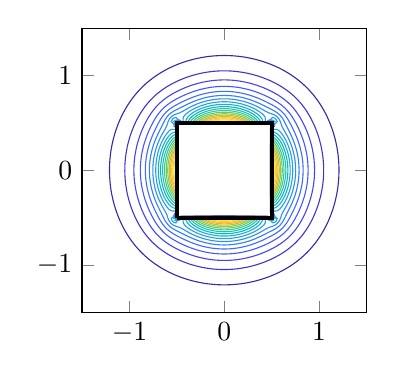
\begin{tikzpicture}

\begin{axis}[%
width=1.422in,
height=1.422in,
at={(0.406in,0.406in)},
scale only axis,
colormap={mymap}{[1pt] rgb(0pt)=(0.2422,0.1504,0.6603); rgb(1pt)=(0.25039,0.164995,0.707614); rgb(2pt)=(0.257771,0.181781,0.751138); rgb(3pt)=(0.264729,0.197757,0.795214); rgb(4pt)=(0.270648,0.214676,0.836371); rgb(5pt)=(0.275114,0.234238,0.870986); rgb(6pt)=(0.2783,0.255871,0.899071); rgb(7pt)=(0.280333,0.278233,0.9221); rgb(8pt)=(0.281338,0.300595,0.941376); rgb(9pt)=(0.281014,0.322757,0.957886); rgb(10pt)=(0.279467,0.344671,0.971676); rgb(11pt)=(0.275971,0.366681,0.982905); rgb(12pt)=(0.269914,0.3892,0.9906); rgb(13pt)=(0.260243,0.412329,0.995157); rgb(14pt)=(0.244033,0.435833,0.998833); rgb(15pt)=(0.220643,0.460257,0.997286); rgb(16pt)=(0.196333,0.484719,0.989152); rgb(17pt)=(0.183405,0.507371,0.979795); rgb(18pt)=(0.178643,0.528857,0.968157); rgb(19pt)=(0.176438,0.549905,0.952019); rgb(20pt)=(0.168743,0.570262,0.935871); rgb(21pt)=(0.154,0.5902,0.9218); rgb(22pt)=(0.146029,0.609119,0.907857); rgb(23pt)=(0.138024,0.627629,0.89729); rgb(24pt)=(0.124814,0.645929,0.888343); rgb(25pt)=(0.111252,0.6635,0.876314); rgb(26pt)=(0.0952095,0.679829,0.859781); rgb(27pt)=(0.0688714,0.694771,0.839357); rgb(28pt)=(0.0296667,0.708167,0.816333); rgb(29pt)=(0.00357143,0.720267,0.7917); rgb(30pt)=(0.00665714,0.731214,0.766014); rgb(31pt)=(0.0433286,0.741095,0.73941); rgb(32pt)=(0.0963952,0.75,0.712038); rgb(33pt)=(0.140771,0.7584,0.684157); rgb(34pt)=(0.1717,0.766962,0.655443); rgb(35pt)=(0.193767,0.775767,0.6251); rgb(36pt)=(0.216086,0.7843,0.5923); rgb(37pt)=(0.246957,0.791795,0.556743); rgb(38pt)=(0.290614,0.79729,0.518829); rgb(39pt)=(0.340643,0.8008,0.478857); rgb(40pt)=(0.3909,0.802871,0.435448); rgb(41pt)=(0.445629,0.802419,0.390919); rgb(42pt)=(0.5044,0.7993,0.348); rgb(43pt)=(0.561562,0.794233,0.304481); rgb(44pt)=(0.617395,0.787619,0.261238); rgb(45pt)=(0.671986,0.779271,0.2227); rgb(46pt)=(0.7242,0.769843,0.191029); rgb(47pt)=(0.773833,0.759805,0.16461); rgb(48pt)=(0.820314,0.749814,0.153529); rgb(49pt)=(0.863433,0.7406,0.159633); rgb(50pt)=(0.903543,0.733029,0.177414); rgb(51pt)=(0.939257,0.728786,0.209957); rgb(52pt)=(0.972757,0.729771,0.239443); rgb(53pt)=(0.995648,0.743371,0.237148); rgb(54pt)=(0.996986,0.765857,0.219943); rgb(55pt)=(0.995205,0.789252,0.202762); rgb(56pt)=(0.9892,0.813567,0.188533); rgb(57pt)=(0.978629,0.838629,0.176557); rgb(58pt)=(0.967648,0.8639,0.16429); rgb(59pt)=(0.96101,0.889019,0.153676); rgb(60pt)=(0.959671,0.913457,0.142257); rgb(61pt)=(0.962795,0.937338,0.12651); rgb(62pt)=(0.969114,0.960629,0.106362); rgb(63pt)=(0.9769,0.9839,0.0805)},
xmin=-1.5000,
xmax=1.5000,
ymin=-1.5000,
ymax=1.5000,
axis background/.style={fill=white}
]
\addplot[contour prepared, contour prepared format=matlab, contour/labels=false] table[row sep=crcr] {%
%
0.0476	393.0000\\
-1.2065	-0.0997\\
-1.2078	-0.0821\\
-1.2092	-0.0572\\
-1.2101	-0.0323\\
-1.2105	-0.0075\\
-1.2105	0.0174\\
-1.2100	0.0423\\
-1.2090	0.0672\\
-1.2075	0.0920\\
-1.2065	0.1046\\
-1.2056	0.1169\\
-1.2033	0.1418\\
-1.2006	0.1667\\
-1.1974	0.1915\\
-1.1936	0.2164\\
-1.1893	0.2413\\
-1.1844	0.2662\\
-1.1816	0.2792\\
-1.1792	0.2910\\
-1.1736	0.3159\\
-1.1674	0.3408\\
-1.1605	0.3657\\
-1.1567	0.3783\\
-1.1532	0.3905\\
-1.1456	0.4154\\
-1.1371	0.4403\\
-1.1318	0.4545\\
-1.1281	0.4652\\
-1.1187	0.4900\\
-1.1083	0.5149\\
-1.1070	0.5180\\
-1.0978	0.5398\\
-1.0862	0.5647\\
-1.0821	0.5730\\
-1.0742	0.5896\\
-1.0612	0.6144\\
-1.0572	0.6216\\
-1.0477	0.6393\\
-1.0330	0.6642\\
-1.0323	0.6653\\
-1.0179	0.6891\\
-1.0075	0.7050\\
-1.0016	0.7139\\
-0.9843	0.7388\\
-0.9826	0.7412\\
-0.9662	0.7637\\
-0.9577	0.7746\\
-0.9468	0.7886\\
-0.9328	0.8054\\
-0.9261	0.8134\\
-0.9080	0.8340\\
-0.9041	0.8383\\
-0.8831	0.8606\\
-0.8805	0.8632\\
-0.8582	0.8854\\
-0.8554	0.8881\\
-0.8333	0.9087\\
-0.8285	0.9129\\
-0.8085	0.9305\\
-0.7996	0.9378\\
-0.7836	0.9510\\
-0.7684	0.9627\\
-0.7587	0.9702\\
-0.7345	0.9876\\
-0.7338	0.9881\\
-0.7090	1.0053\\
-0.6979	1.0124\\
-0.6841	1.0214\\
-0.6592	1.0364\\
-0.6576	1.0373\\
-0.6343	1.0509\\
-0.6132	1.0622\\
-0.6095	1.0643\\
-0.5846	1.0772\\
-0.5638	1.0871\\
-0.5597	1.0891\\
-0.5348	1.1006\\
-0.5100	1.1111\\
-0.5077	1.1119\\
-0.4851	1.1214\\
-0.4602	1.1308\\
-0.4428	1.1368\\
-0.4353	1.1395\\
-0.4104	1.1480\\
-0.3856	1.1557\\
-0.3642	1.1617\\
-0.3607	1.1627\\
-0.3358	1.1697\\
-0.3109	1.1759\\
-0.2861	1.1814\\
-0.2612	1.1864\\
-0.2603	1.1866\\
-0.2363	1.1913\\
-0.2114	1.1956\\
-0.1866	1.1993\\
-0.1617	1.2025\\
-0.1368	1.2052\\
-0.1119	1.2075\\
-0.0871	1.2093\\
-0.0622	1.2106\\
-0.0374	1.2114\\
-0.0373	1.2114\\
-0.0124	1.2119\\
0.0124	1.2119\\
0.0373	1.2114\\
0.0374	1.2114\\
0.0622	1.2106\\
0.0871	1.2093\\
0.1119	1.2075\\
0.1368	1.2052\\
0.1617	1.2025\\
0.1866	1.1993\\
0.2114	1.1956\\
0.2363	1.1913\\
0.2603	1.1866\\
0.2612	1.1864\\
0.2861	1.1814\\
0.3109	1.1759\\
0.3358	1.1697\\
0.3607	1.1627\\
0.3642	1.1617\\
0.3856	1.1557\\
0.4104	1.1480\\
0.4353	1.1395\\
0.4428	1.1368\\
0.4602	1.1308\\
0.4851	1.1214\\
0.5077	1.1119\\
0.5100	1.1111\\
0.5348	1.1006\\
0.5597	1.0891\\
0.5638	1.0871\\
0.5846	1.0772\\
0.6095	1.0643\\
0.6132	1.0622\\
0.6343	1.0509\\
0.6576	1.0373\\
0.6592	1.0364\\
0.6841	1.0214\\
0.6979	1.0124\\
0.7090	1.0053\\
0.7338	0.9881\\
0.7345	0.9876\\
0.7587	0.9702\\
0.7684	0.9627\\
0.7836	0.9510\\
0.7996	0.9378\\
0.8085	0.9305\\
0.8285	0.9129\\
0.8333	0.9087\\
0.8554	0.8881\\
0.8582	0.8854\\
0.8805	0.8632\\
0.8831	0.8606\\
0.9041	0.8383\\
0.9080	0.8340\\
0.9261	0.8134\\
0.9328	0.8054\\
0.9468	0.7886\\
0.9577	0.7746\\
0.9662	0.7637\\
0.9826	0.7412\\
0.9843	0.7388\\
1.0016	0.7139\\
1.0075	0.7050\\
1.0179	0.6891\\
1.0323	0.6653\\
1.0330	0.6642\\
1.0477	0.6393\\
1.0572	0.6216\\
1.0612	0.6144\\
1.0742	0.5896\\
1.0821	0.5730\\
1.0862	0.5647\\
1.0978	0.5398\\
1.1070	0.5180\\
1.1083	0.5149\\
1.1187	0.4900\\
1.1281	0.4652\\
1.1318	0.4545\\
1.1371	0.4403\\
1.1456	0.4154\\
1.1532	0.3905\\
1.1567	0.3783\\
1.1605	0.3657\\
1.1674	0.3408\\
1.1736	0.3159\\
1.1792	0.2910\\
1.1816	0.2792\\
1.1844	0.2662\\
1.1893	0.2413\\
1.1936	0.2164\\
1.1974	0.1915\\
1.2006	0.1667\\
1.2033	0.1418\\
1.2056	0.1169\\
1.2065	0.1046\\
1.2075	0.0920\\
1.2090	0.0672\\
1.2100	0.0423\\
1.2105	0.0174\\
1.2105	-0.0075\\
1.2101	-0.0323\\
1.2092	-0.0572\\
1.2078	-0.0821\\
1.2065	-0.0997\\
1.2060	-0.1070\\
1.2038	-0.1318\\
1.2012	-0.1567\\
1.1980	-0.1816\\
1.1944	-0.2065\\
1.1902	-0.2313\\
1.1855	-0.2562\\
1.1816	-0.2743\\
1.1802	-0.2811\\
1.1748	-0.3060\\
1.1687	-0.3308\\
1.1620	-0.3557\\
1.1567	-0.3734\\
1.1547	-0.3806\\
1.1472	-0.4055\\
1.1389	-0.4303\\
1.1318	-0.4496\\
1.1299	-0.4552\\
1.1207	-0.4801\\
1.1105	-0.5050\\
1.1070	-0.5130\\
1.0999	-0.5299\\
1.0886	-0.5547\\
1.0821	-0.5680\\
1.0766	-0.5796\\
1.0639	-0.6045\\
1.0572	-0.6166\\
1.0504	-0.6294\\
1.0361	-0.6542\\
1.0323	-0.6603\\
1.0211	-0.6791\\
1.0075	-0.7000\\
1.0049	-0.7040\\
0.9879	-0.7289\\
0.9826	-0.7362\\
0.9700	-0.7537\\
0.9577	-0.7696\\
0.9507	-0.7786\\
0.9328	-0.8004\\
0.9303	-0.8035\\
0.9085	-0.8284\\
0.9080	-0.8289\\
0.8854	-0.8532\\
0.8831	-0.8556\\
0.8606	-0.8781\\
0.8582	-0.8804\\
0.8340	-0.9030\\
0.8333	-0.9036\\
0.8085	-0.9254\\
0.8055	-0.9279\\
0.7836	-0.9460\\
0.7749	-0.9527\\
0.7587	-0.9652\\
0.7416	-0.9776\\
0.7338	-0.9833\\
0.7090	-1.0002\\
0.7054	-1.0025\\
0.6841	-1.0165\\
0.6660	-1.0274\\
0.6592	-1.0315\\
0.6343	-1.0459\\
0.6225	-1.0522\\
0.6095	-1.0594\\
0.5846	-1.0721\\
0.5741	-1.0771\\
0.5597	-1.0842\\
0.5348	-1.0956\\
0.5196	-1.1020\\
0.5100	-1.1062\\
0.4851	-1.1164\\
0.4602	-1.1256\\
0.4567	-1.1269\\
0.4353	-1.1347\\
0.4104	-1.1430\\
0.3856	-1.1506\\
0.3814	-1.1517\\
0.3607	-1.1579\\
0.3358	-1.1647\\
0.3109	-1.1708\\
0.2861	-1.1763\\
0.2843	-1.1766\\
0.2612	-1.1816\\
0.2363	-1.1864\\
0.2114	-1.1906\\
0.1866	-1.1943\\
0.1617	-1.1974\\
0.1368	-1.2001\\
0.1210	-1.2015\\
0.1119	-1.2024\\
0.0871	-1.2043\\
0.0622	-1.2057\\
0.0373	-1.2067\\
0.0124	-1.2071\\
-0.0124	-1.2071\\
-0.0373	-1.2067\\
-0.0622	-1.2057\\
-0.0871	-1.2043\\
-0.1119	-1.2024\\
-0.1210	-1.2015\\
-0.1368	-1.2001\\
-0.1617	-1.1974\\
-0.1866	-1.1943\\
-0.2114	-1.1906\\
-0.2363	-1.1864\\
-0.2612	-1.1816\\
-0.2843	-1.1766\\
-0.2861	-1.1763\\
-0.3109	-1.1708\\
-0.3358	-1.1647\\
-0.3607	-1.1579\\
-0.3814	-1.1517\\
-0.3856	-1.1506\\
-0.4104	-1.1430\\
-0.4353	-1.1347\\
-0.4567	-1.1269\\
-0.4602	-1.1256\\
-0.4851	-1.1164\\
-0.5100	-1.1062\\
-0.5196	-1.1020\\
-0.5348	-1.0956\\
-0.5597	-1.0842\\
-0.5741	-1.0771\\
-0.5846	-1.0721\\
-0.6095	-1.0594\\
-0.6225	-1.0522\\
-0.6343	-1.0459\\
-0.6592	-1.0315\\
-0.6660	-1.0274\\
-0.6841	-1.0165\\
-0.7054	-1.0025\\
-0.7090	-1.0002\\
-0.7338	-0.9833\\
-0.7416	-0.9776\\
-0.7587	-0.9652\\
-0.7749	-0.9527\\
-0.7836	-0.9460\\
-0.8055	-0.9279\\
-0.8085	-0.9254\\
-0.8333	-0.9036\\
-0.8340	-0.9030\\
-0.8582	-0.8804\\
-0.8606	-0.8781\\
-0.8831	-0.8556\\
-0.8854	-0.8532\\
-0.9080	-0.8289\\
-0.9085	-0.8284\\
-0.9303	-0.8035\\
-0.9328	-0.8004\\
-0.9507	-0.7786\\
-0.9577	-0.7696\\
-0.9700	-0.7537\\
-0.9826	-0.7362\\
-0.9879	-0.7289\\
-1.0049	-0.7040\\
-1.0075	-0.7000\\
-1.0211	-0.6791\\
-1.0323	-0.6603\\
-1.0361	-0.6542\\
-1.0504	-0.6294\\
-1.0572	-0.6166\\
-1.0639	-0.6045\\
-1.0766	-0.5796\\
-1.0821	-0.5680\\
-1.0886	-0.5547\\
-1.0999	-0.5299\\
-1.1070	-0.5130\\
-1.1105	-0.5050\\
-1.1207	-0.4801\\
-1.1299	-0.4552\\
-1.1318	-0.4496\\
-1.1389	-0.4303\\
-1.1472	-0.4055\\
-1.1547	-0.3806\\
-1.1567	-0.3734\\
-1.1620	-0.3557\\
-1.1687	-0.3308\\
-1.1748	-0.3060\\
-1.1802	-0.2811\\
-1.1816	-0.2743\\
-1.1855	-0.2562\\
-1.1902	-0.2313\\
-1.1944	-0.2065\\
-1.1980	-0.1816\\
-1.2012	-0.1567\\
-1.2038	-0.1318\\
-1.2060	-0.1070\\
-1.2065	-0.0997\\
0.0476	169.0000\\
-0.5100	-0.4793\\
-0.5106	-0.4801\\
-0.5100	-0.4810\\
-0.4860	-0.5050\\
-0.4851	-0.5057\\
-0.4842	-0.5050\\
-0.4602	-0.4838\\
-0.4353	-0.4833\\
-0.4104	-0.4829\\
-0.3856	-0.4826\\
-0.3607	-0.4824\\
-0.3358	-0.4822\\
-0.3109	-0.4820\\
-0.2861	-0.4819\\
-0.2612	-0.4817\\
-0.2363	-0.4816\\
-0.2114	-0.4816\\
-0.1866	-0.4815\\
-0.1617	-0.4814\\
-0.1368	-0.4814\\
-0.1119	-0.4814\\
-0.0871	-0.4813\\
-0.0622	-0.4813\\
-0.0373	-0.4813\\
-0.0124	-0.4813\\
0.0124	-0.4813\\
0.0373	-0.4813\\
0.0622	-0.4813\\
0.0871	-0.4813\\
0.1119	-0.4814\\
0.1368	-0.4814\\
0.1617	-0.4814\\
0.1866	-0.4815\\
0.2114	-0.4816\\
0.2363	-0.4816\\
0.2612	-0.4817\\
0.2861	-0.4819\\
0.3109	-0.4820\\
0.3358	-0.4822\\
0.3607	-0.4824\\
0.3856	-0.4826\\
0.4104	-0.4829\\
0.4353	-0.4833\\
0.4602	-0.4838\\
0.4842	-0.5050\\
0.4851	-0.5057\\
0.4860	-0.5050\\
0.5100	-0.4810\\
0.5106	-0.4801\\
0.5100	-0.4793\\
0.4888	-0.4552\\
0.4882	-0.4303\\
0.4879	-0.4055\\
0.4876	-0.3806\\
0.4873	-0.3557\\
0.4871	-0.3308\\
0.4870	-0.3060\\
0.4868	-0.2811\\
0.4867	-0.2562\\
0.4866	-0.2313\\
0.4865	-0.2065\\
0.4865	-0.1816\\
0.4864	-0.1567\\
0.4864	-0.1318\\
0.4863	-0.1070\\
0.4863	-0.0821\\
0.4863	-0.0572\\
0.4863	-0.0323\\
0.4863	-0.0075\\
0.4863	0.0174\\
0.4863	0.0423\\
0.4863	0.0672\\
0.4863	0.0920\\
0.4863	0.1169\\
0.4864	0.1418\\
0.4864	0.1667\\
0.4865	0.1915\\
0.4866	0.2164\\
0.4866	0.2413\\
0.4867	0.2662\\
0.4869	0.2910\\
0.4870	0.3159\\
0.4872	0.3408\\
0.4874	0.3657\\
0.4876	0.3905\\
0.4879	0.4154\\
0.4883	0.4403\\
0.4891	0.4652\\
0.4941	0.4900\\
0.4851	0.4976\\
0.4602	0.4938\\
0.4353	0.4932\\
0.4104	0.4929\\
0.3856	0.4926\\
0.3607	0.4923\\
0.3358	0.4921\\
0.3109	0.4920\\
0.2861	0.4918\\
0.2612	0.4917\\
0.2363	0.4916\\
0.2114	0.4915\\
0.1866	0.4915\\
0.1617	0.4914\\
0.1368	0.4914\\
0.1119	0.4913\\
0.0871	0.4913\\
0.0622	0.4913\\
0.0373	0.4913\\
0.0124	0.4913\\
-0.0124	0.4913\\
-0.0373	0.4913\\
-0.0622	0.4913\\
-0.0871	0.4913\\
-0.1119	0.4913\\
-0.1368	0.4914\\
-0.1617	0.4914\\
-0.1866	0.4915\\
-0.2114	0.4915\\
-0.2363	0.4916\\
-0.2612	0.4917\\
-0.2861	0.4918\\
-0.3109	0.4920\\
-0.3358	0.4921\\
-0.3607	0.4923\\
-0.3856	0.4926\\
-0.4104	0.4929\\
-0.4353	0.4932\\
-0.4602	0.4938\\
-0.4851	0.4976\\
-0.4941	0.4900\\
-0.4891	0.4652\\
-0.4883	0.4403\\
-0.4879	0.4154\\
-0.4876	0.3905\\
-0.4874	0.3657\\
-0.4872	0.3408\\
-0.4870	0.3159\\
-0.4869	0.2910\\
-0.4867	0.2662\\
-0.4866	0.2413\\
-0.4866	0.2164\\
-0.4865	0.1915\\
-0.4864	0.1667\\
-0.4864	0.1418\\
-0.4863	0.1169\\
-0.4863	0.0920\\
-0.4863	0.0672\\
-0.4863	0.0423\\
-0.4863	0.0174\\
-0.4863	-0.0075\\
-0.4863	-0.0323\\
-0.4863	-0.0572\\
-0.4863	-0.0821\\
-0.4863	-0.1070\\
-0.4864	-0.1318\\
-0.4864	-0.1567\\
-0.4865	-0.1816\\
-0.4865	-0.2065\\
-0.4866	-0.2313\\
-0.4867	-0.2562\\
-0.4868	-0.2811\\
-0.4870	-0.3060\\
-0.4871	-0.3308\\
-0.4873	-0.3557\\
-0.4876	-0.3806\\
-0.4879	-0.4055\\
-0.4882	-0.4303\\
-0.4888	-0.4552\\
-0.5100	-0.4793\\
0.0952	337.0000\\
-1.0323	-0.1925\\
-1.0343	-0.1816\\
-1.0380	-0.1567\\
-1.0412	-0.1318\\
-1.0439	-0.1070\\
-1.0459	-0.0821\\
-1.0474	-0.0572\\
-1.0484	-0.0323\\
-1.0489	-0.0075\\
-1.0488	0.0174\\
-1.0483	0.0423\\
-1.0472	0.0672\\
-1.0455	0.0920\\
-1.0434	0.1169\\
-1.0406	0.1418\\
-1.0373	0.1667\\
-1.0334	0.1915\\
-1.0323	0.1975\\
-1.0292	0.2164\\
-1.0245	0.2413\\
-1.0191	0.2662\\
-1.0130	0.2910\\
-1.0075	0.3113\\
-1.0063	0.3159\\
-0.9994	0.3408\\
-0.9916	0.3657\\
-0.9831	0.3905\\
-0.9826	0.3918\\
-0.9743	0.4154\\
-0.9647	0.4403\\
-0.9577	0.4568\\
-0.9543	0.4652\\
-0.9435	0.4900\\
-0.9328	0.5121\\
-0.9315	0.5149\\
-0.9192	0.5398\\
-0.9080	0.5603\\
-0.9057	0.5647\\
-0.8915	0.5896\\
-0.8831	0.6032\\
-0.8762	0.6144\\
-0.8597	0.6393\\
-0.8582	0.6414\\
-0.8423	0.6642\\
-0.8333	0.6760\\
-0.8233	0.6891\\
-0.8085	0.7072\\
-0.8028	0.7139\\
-0.7836	0.7355\\
-0.7806	0.7388\\
-0.7587	0.7615\\
-0.7565	0.7637\\
-0.7338	0.7852\\
-0.7302	0.7886\\
-0.7090	0.8072\\
-0.7014	0.8134\\
-0.6841	0.8274\\
-0.6697	0.8383\\
-0.6592	0.8461\\
-0.6345	0.8632\\
-0.6343	0.8633\\
-0.6095	0.8797\\
-0.5956	0.8881\\
-0.5846	0.8948\\
-0.5597	0.9089\\
-0.5521	0.9129\\
-0.5348	0.9223\\
-0.5100	0.9346\\
-0.5029	0.9378\\
-0.4851	0.9463\\
-0.4602	0.9572\\
-0.4464	0.9627\\
-0.4353	0.9673\\
-0.4104	0.9770\\
-0.3856	0.9857\\
-0.3798	0.9876\\
-0.3607	0.9941\\
-0.3358	1.0018\\
-0.3109	1.0088\\
-0.2963	1.0124\\
-0.2861	1.0152\\
-0.2612	1.0213\\
-0.2363	1.0267\\
-0.2114	1.0314\\
-0.1866	1.0355\\
-0.1740	1.0373\\
-0.1617	1.0392\\
-0.1368	1.0425\\
-0.1119	1.0452\\
-0.0871	1.0474\\
-0.0622	1.0490\\
-0.0373	1.0500\\
-0.0124	1.0506\\
0.0124	1.0506\\
0.0373	1.0500\\
0.0622	1.0490\\
0.0871	1.0474\\
0.1119	1.0452\\
0.1368	1.0425\\
0.1617	1.0392\\
0.1740	1.0373\\
0.1866	1.0355\\
0.2114	1.0314\\
0.2363	1.0267\\
0.2612	1.0213\\
0.2861	1.0152\\
0.2963	1.0124\\
0.3109	1.0088\\
0.3358	1.0018\\
0.3607	0.9941\\
0.3798	0.9876\\
0.3856	0.9857\\
0.4104	0.9770\\
0.4353	0.9673\\
0.4464	0.9627\\
0.4602	0.9572\\
0.4851	0.9463\\
0.5029	0.9378\\
0.5100	0.9346\\
0.5348	0.9223\\
0.5521	0.9129\\
0.5597	0.9089\\
0.5846	0.8948\\
0.5956	0.8881\\
0.6095	0.8797\\
0.6343	0.8633\\
0.6345	0.8632\\
0.6592	0.8461\\
0.6697	0.8383\\
0.6841	0.8274\\
0.7014	0.8134\\
0.7090	0.8072\\
0.7302	0.7886\\
0.7338	0.7852\\
0.7565	0.7637\\
0.7587	0.7615\\
0.7806	0.7388\\
0.7836	0.7355\\
0.8028	0.7139\\
0.8085	0.7072\\
0.8233	0.6891\\
0.8333	0.6760\\
0.8423	0.6642\\
0.8582	0.6414\\
0.8597	0.6393\\
0.8762	0.6144\\
0.8831	0.6032\\
0.8915	0.5896\\
0.9057	0.5647\\
0.9080	0.5603\\
0.9192	0.5398\\
0.9315	0.5149\\
0.9328	0.5121\\
0.9435	0.4900\\
0.9543	0.4652\\
0.9577	0.4568\\
0.9647	0.4403\\
0.9743	0.4154\\
0.9826	0.3918\\
0.9831	0.3905\\
0.9916	0.3657\\
0.9994	0.3408\\
1.0063	0.3159\\
1.0075	0.3113\\
1.0130	0.2910\\
1.0191	0.2662\\
1.0245	0.2413\\
1.0292	0.2164\\
1.0323	0.1975\\
1.0334	0.1915\\
1.0373	0.1667\\
1.0406	0.1418\\
1.0434	0.1169\\
1.0455	0.0920\\
1.0472	0.0672\\
1.0483	0.0423\\
1.0488	0.0174\\
1.0489	-0.0075\\
1.0484	-0.0323\\
1.0474	-0.0572\\
1.0459	-0.0821\\
1.0439	-0.1070\\
1.0412	-0.1318\\
1.0380	-0.1567\\
1.0343	-0.1816\\
1.0323	-0.1925\\
1.0301	-0.2065\\
1.0255	-0.2313\\
1.0202	-0.2562\\
1.0143	-0.2811\\
1.0076	-0.3060\\
1.0075	-0.3064\\
1.0008	-0.3308\\
0.9933	-0.3557\\
0.9848	-0.3806\\
0.9826	-0.3868\\
0.9761	-0.4055\\
0.9667	-0.4303\\
0.9577	-0.4518\\
0.9563	-0.4552\\
0.9457	-0.4801\\
0.9339	-0.5050\\
0.9328	-0.5071\\
0.9218	-0.5299\\
0.9083	-0.5547\\
0.9080	-0.5554\\
0.8945	-0.5796\\
0.8831	-0.5982\\
0.8793	-0.6045\\
0.8632	-0.6294\\
0.8582	-0.6365\\
0.8459	-0.6542\\
0.8333	-0.6710\\
0.8272	-0.6791\\
0.8085	-0.7021\\
0.8069	-0.7040\\
0.7851	-0.7289\\
0.7836	-0.7305\\
0.7615	-0.7537\\
0.7587	-0.7565\\
0.7356	-0.7786\\
0.7338	-0.7802\\
0.7090	-0.8021\\
0.7073	-0.8035\\
0.6841	-0.8224\\
0.6762	-0.8284\\
0.6592	-0.8412\\
0.6419	-0.8532\\
0.6343	-0.8585\\
0.6095	-0.8747\\
0.6037	-0.8781\\
0.5846	-0.8899\\
0.5612	-0.9030\\
0.5597	-0.9038\\
0.5348	-0.9173\\
0.5132	-0.9279\\
0.5100	-0.9295\\
0.4851	-0.9414\\
0.4602	-0.9520\\
0.4584	-0.9527\\
0.4353	-0.9625\\
0.4104	-0.9719\\
0.3941	-0.9776\\
0.3856	-0.9807\\
0.3607	-0.9892\\
0.3358	-0.9968\\
0.3150	-1.0025\\
0.3109	-1.0037\\
0.2861	-1.0104\\
0.2612	-1.0163\\
0.2363	-1.0216\\
0.2114	-1.0263\\
0.2047	-1.0274\\
0.1866	-1.0306\\
0.1617	-1.0344\\
0.1368	-1.0377\\
0.1119	-1.0403\\
0.0871	-1.0424\\
0.0622	-1.0440\\
0.0373	-1.0450\\
0.0124	-1.0455\\
-0.0124	-1.0455\\
-0.0373	-1.0450\\
-0.0622	-1.0440\\
-0.0871	-1.0424\\
-0.1119	-1.0403\\
-0.1368	-1.0377\\
-0.1617	-1.0344\\
-0.1866	-1.0306\\
-0.2047	-1.0274\\
-0.2114	-1.0263\\
-0.2363	-1.0216\\
-0.2612	-1.0163\\
-0.2861	-1.0104\\
-0.3109	-1.0037\\
-0.3150	-1.0025\\
-0.3358	-0.9968\\
-0.3607	-0.9892\\
-0.3856	-0.9807\\
-0.3941	-0.9776\\
-0.4104	-0.9719\\
-0.4353	-0.9625\\
-0.4584	-0.9527\\
-0.4602	-0.9520\\
-0.4851	-0.9414\\
-0.5100	-0.9295\\
-0.5132	-0.9279\\
-0.5348	-0.9173\\
-0.5597	-0.9038\\
-0.5612	-0.9030\\
-0.5846	-0.8899\\
-0.6037	-0.8781\\
-0.6095	-0.8747\\
-0.6343	-0.8585\\
-0.6419	-0.8532\\
-0.6592	-0.8412\\
-0.6762	-0.8284\\
-0.6841	-0.8224\\
-0.7073	-0.8035\\
-0.7090	-0.8021\\
-0.7338	-0.7802\\
-0.7356	-0.7786\\
-0.7587	-0.7565\\
-0.7615	-0.7537\\
-0.7836	-0.7305\\
-0.7851	-0.7289\\
-0.8069	-0.7040\\
-0.8085	-0.7021\\
-0.8272	-0.6791\\
-0.8333	-0.6710\\
-0.8459	-0.6542\\
-0.8582	-0.6365\\
-0.8632	-0.6294\\
-0.8793	-0.6045\\
-0.8831	-0.5982\\
-0.8945	-0.5796\\
-0.9080	-0.5554\\
-0.9083	-0.5547\\
-0.9218	-0.5299\\
-0.9328	-0.5071\\
-0.9339	-0.5050\\
-0.9457	-0.4801\\
-0.9563	-0.4552\\
-0.9577	-0.4518\\
-0.9667	-0.4303\\
-0.9761	-0.4055\\
-0.9826	-0.3868\\
-0.9848	-0.3806\\
-0.9933	-0.3557\\
-1.0008	-0.3308\\
-1.0075	-0.3064\\
-1.0076	-0.3060\\
-1.0143	-0.2811\\
-1.0202	-0.2562\\
-1.0255	-0.2313\\
-1.0301	-0.2065\\
-1.0323	-0.1925\\
0.0952	169.0000\\
-0.5100	-0.4750\\
-0.5143	-0.4801\\
-0.5100	-0.4856\\
-0.4906	-0.5050\\
-0.4851	-0.5094\\
-0.4800	-0.5050\\
-0.4602	-0.4876\\
-0.4353	-0.4864\\
-0.4104	-0.4857\\
-0.3856	-0.4851\\
-0.3607	-0.4846\\
-0.3358	-0.4842\\
-0.3109	-0.4839\\
-0.2861	-0.4836\\
-0.2612	-0.4834\\
-0.2363	-0.4832\\
-0.2114	-0.4830\\
-0.1866	-0.4829\\
-0.1617	-0.4828\\
-0.1368	-0.4827\\
-0.1119	-0.4826\\
-0.0871	-0.4826\\
-0.0622	-0.4825\\
-0.0373	-0.4825\\
-0.0124	-0.4825\\
0.0124	-0.4825\\
0.0373	-0.4825\\
0.0622	-0.4825\\
0.0871	-0.4826\\
0.1119	-0.4826\\
0.1368	-0.4827\\
0.1617	-0.4828\\
0.1866	-0.4829\\
0.2114	-0.4830\\
0.2363	-0.4832\\
0.2612	-0.4834\\
0.2861	-0.4836\\
0.3109	-0.4839\\
0.3358	-0.4842\\
0.3607	-0.4846\\
0.3856	-0.4851\\
0.4104	-0.4857\\
0.4353	-0.4864\\
0.4602	-0.4876\\
0.4800	-0.5050\\
0.4851	-0.5094\\
0.4906	-0.5050\\
0.5100	-0.4856\\
0.5143	-0.4801\\
0.5100	-0.4750\\
0.4926	-0.4552\\
0.4914	-0.4303\\
0.4907	-0.4055\\
0.4901	-0.3806\\
0.4896	-0.3557\\
0.4892	-0.3308\\
0.4889	-0.3060\\
0.4886	-0.2811\\
0.4884	-0.2562\\
0.4882	-0.2313\\
0.4880	-0.2065\\
0.4879	-0.1816\\
0.4878	-0.1567\\
0.4877	-0.1318\\
0.4876	-0.1070\\
0.4875	-0.0821\\
0.4875	-0.0572\\
0.4875	-0.0323\\
0.4875	-0.0075\\
0.4875	0.0174\\
0.4875	0.0423\\
0.4875	0.0672\\
0.4876	0.0920\\
0.4876	0.1169\\
0.4877	0.1418\\
0.4878	0.1667\\
0.4879	0.1915\\
0.4880	0.2164\\
0.4882	0.2413\\
0.4884	0.2662\\
0.4887	0.2910\\
0.4889	0.3159\\
0.4893	0.3408\\
0.4897	0.3657\\
0.4902	0.3905\\
0.4908	0.4154\\
0.4916	0.4403\\
0.4930	0.4652\\
0.5031	0.4900\\
0.4851	0.5051\\
0.4602	0.4975\\
0.4353	0.4964\\
0.4104	0.4957\\
0.3856	0.4951\\
0.3607	0.4946\\
0.3358	0.4942\\
0.3109	0.4939\\
0.2861	0.4936\\
0.2612	0.4934\\
0.2363	0.4932\\
0.2114	0.4930\\
0.1866	0.4929\\
0.1617	0.4928\\
0.1368	0.4927\\
0.1119	0.4926\\
0.0871	0.4926\\
0.0622	0.4925\\
0.0373	0.4925\\
0.0124	0.4925\\
-0.0124	0.4925\\
-0.0373	0.4925\\
-0.0622	0.4925\\
-0.0871	0.4926\\
-0.1119	0.4926\\
-0.1368	0.4927\\
-0.1617	0.4928\\
-0.1866	0.4929\\
-0.2114	0.4930\\
-0.2363	0.4932\\
-0.2612	0.4934\\
-0.2861	0.4936\\
-0.3109	0.4939\\
-0.3358	0.4942\\
-0.3607	0.4946\\
-0.3856	0.4951\\
-0.4104	0.4957\\
-0.4353	0.4964\\
-0.4602	0.4975\\
-0.4851	0.5051\\
-0.5031	0.4900\\
-0.4930	0.4652\\
-0.4916	0.4403\\
-0.4908	0.4154\\
-0.4902	0.3905\\
-0.4897	0.3657\\
-0.4893	0.3408\\
-0.4889	0.3159\\
-0.4887	0.2910\\
-0.4884	0.2662\\
-0.4882	0.2413\\
-0.4880	0.2164\\
-0.4879	0.1915\\
-0.4878	0.1667\\
-0.4877	0.1418\\
-0.4876	0.1169\\
-0.4876	0.0920\\
-0.4875	0.0672\\
-0.4875	0.0423\\
-0.4875	0.0174\\
-0.4875	-0.0075\\
-0.4875	-0.0323\\
-0.4875	-0.0572\\
-0.4875	-0.0821\\
-0.4876	-0.1070\\
-0.4877	-0.1318\\
-0.4878	-0.1567\\
-0.4879	-0.1816\\
-0.4880	-0.2065\\
-0.4882	-0.2313\\
-0.4884	-0.2562\\
-0.4886	-0.2811\\
-0.4889	-0.3060\\
-0.4892	-0.3308\\
-0.4896	-0.3557\\
-0.4901	-0.3806\\
-0.4907	-0.4055\\
-0.4914	-0.4303\\
-0.4926	-0.4552\\
-0.5100	-0.4750\\
0.1429	305.0000\\
-0.9328	-0.2028\\
-0.9369	-0.1816\\
-0.9411	-0.1567\\
-0.9446	-0.1318\\
-0.9474	-0.1070\\
-0.9497	-0.0821\\
-0.9513	-0.0572\\
-0.9524	-0.0323\\
-0.9529	-0.0075\\
-0.9529	0.0174\\
-0.9522	0.0423\\
-0.9511	0.0672\\
-0.9493	0.0920\\
-0.9469	0.1169\\
-0.9439	0.1418\\
-0.9403	0.1667\\
-0.9360	0.1915\\
-0.9328	0.2076\\
-0.9312	0.2164\\
-0.9260	0.2413\\
-0.9201	0.2662\\
-0.9134	0.2910\\
-0.9080	0.3093\\
-0.9061	0.3159\\
-0.8985	0.3408\\
-0.8899	0.3657\\
-0.8831	0.3839\\
-0.8807	0.3905\\
-0.8711	0.4154\\
-0.8604	0.4403\\
-0.8582	0.4452\\
-0.8494	0.4652\\
-0.8374	0.4900\\
-0.8333	0.4978\\
-0.8247	0.5149\\
-0.8109	0.5398\\
-0.8085	0.5439\\
-0.7964	0.5647\\
-0.7836	0.5845\\
-0.7804	0.5896\\
-0.7632	0.6144\\
-0.7587	0.6205\\
-0.7445	0.6393\\
-0.7338	0.6523\\
-0.7238	0.6642\\
-0.7090	0.6805\\
-0.7008	0.6891\\
-0.6841	0.7056\\
-0.6752	0.7139\\
-0.6592	0.7282\\
-0.6464	0.7388\\
-0.6343	0.7486\\
-0.6139	0.7637\\
-0.6095	0.7670\\
-0.5846	0.7840\\
-0.5773	0.7886\\
-0.5597	0.7998\\
-0.5359	0.8134\\
-0.5348	0.8141\\
-0.5100	0.8278\\
-0.4890	0.8383\\
-0.4851	0.8403\\
-0.4602	0.8524\\
-0.4353	0.8632\\
-0.4353	0.8632\\
-0.4104	0.8738\\
-0.3856	0.8835\\
-0.3726	0.8881\\
-0.3607	0.8925\\
-0.3358	0.9010\\
-0.3109	0.9087\\
-0.2956	0.9129\\
-0.2861	0.9158\\
-0.2612	0.9224\\
-0.2363	0.9284\\
-0.2114	0.9335\\
-0.1879	0.9378\\
-0.1866	0.9381\\
-0.1617	0.9423\\
-0.1368	0.9459\\
-0.1119	0.9489\\
-0.0871	0.9512\\
-0.0622	0.9530\\
-0.0373	0.9541\\
-0.0124	0.9547\\
0.0124	0.9547\\
0.0373	0.9541\\
0.0622	0.9530\\
0.0871	0.9512\\
0.1119	0.9489\\
0.1368	0.9459\\
0.1617	0.9423\\
0.1866	0.9381\\
0.1879	0.9378\\
0.2114	0.9335\\
0.2363	0.9284\\
0.2612	0.9224\\
0.2861	0.9158\\
0.2956	0.9129\\
0.3109	0.9087\\
0.3358	0.9010\\
0.3607	0.8925\\
0.3726	0.8881\\
0.3856	0.8835\\
0.4104	0.8738\\
0.4353	0.8632\\
0.4353	0.8632\\
0.4602	0.8524\\
0.4851	0.8403\\
0.4890	0.8383\\
0.5100	0.8278\\
0.5348	0.8141\\
0.5359	0.8134\\
0.5597	0.7998\\
0.5773	0.7886\\
0.5846	0.7840\\
0.6095	0.7670\\
0.6139	0.7637\\
0.6343	0.7486\\
0.6464	0.7388\\
0.6592	0.7282\\
0.6752	0.7139\\
0.6841	0.7056\\
0.7008	0.6891\\
0.7090	0.6805\\
0.7238	0.6642\\
0.7338	0.6523\\
0.7445	0.6393\\
0.7587	0.6205\\
0.7632	0.6144\\
0.7804	0.5896\\
0.7836	0.5845\\
0.7964	0.5647\\
0.8085	0.5439\\
0.8109	0.5398\\
0.8247	0.5149\\
0.8333	0.4978\\
0.8374	0.4900\\
0.8494	0.4652\\
0.8582	0.4452\\
0.8604	0.4403\\
0.8711	0.4154\\
0.8807	0.3905\\
0.8831	0.3839\\
0.8899	0.3657\\
0.8985	0.3408\\
0.9061	0.3159\\
0.9080	0.3093\\
0.9134	0.2910\\
0.9201	0.2662\\
0.9260	0.2413\\
0.9312	0.2164\\
0.9328	0.2076\\
0.9360	0.1915\\
0.9403	0.1667\\
0.9439	0.1418\\
0.9469	0.1169\\
0.9493	0.0920\\
0.9511	0.0672\\
0.9522	0.0423\\
0.9529	0.0174\\
0.9529	-0.0075\\
0.9524	-0.0323\\
0.9513	-0.0572\\
0.9497	-0.0821\\
0.9474	-0.1070\\
0.9446	-0.1318\\
0.9411	-0.1567\\
0.9369	-0.1816\\
0.9328	-0.2028\\
0.9322	-0.2065\\
0.9271	-0.2313\\
0.9213	-0.2562\\
0.9148	-0.2811\\
0.9080	-0.3044\\
0.9075	-0.3060\\
0.9001	-0.3308\\
0.8917	-0.3557\\
0.8831	-0.3790\\
0.8825	-0.3806\\
0.8731	-0.4055\\
0.8627	-0.4303\\
0.8582	-0.4402\\
0.8517	-0.4552\\
0.8399	-0.4801\\
0.8333	-0.4928\\
0.8273	-0.5050\\
0.8138	-0.5299\\
0.8085	-0.5389\\
0.7994	-0.5547\\
0.7836	-0.5796\\
0.7836	-0.5796\\
0.7669	-0.6045\\
0.7587	-0.6155\\
0.7484	-0.6294\\
0.7338	-0.6473\\
0.7280	-0.6542\\
0.7090	-0.6754\\
0.7055	-0.6791\\
0.6841	-0.7006\\
0.6805	-0.7040\\
0.6592	-0.7232\\
0.6524	-0.7289\\
0.6343	-0.7436\\
0.6208	-0.7537\\
0.6095	-0.7621\\
0.5850	-0.7786\\
0.5846	-0.7789\\
0.5597	-0.7948\\
0.5446	-0.8035\\
0.5348	-0.8092\\
0.5100	-0.8228\\
0.4988	-0.8284\\
0.4851	-0.8355\\
0.4602	-0.8473\\
0.4466	-0.8532\\
0.4353	-0.8584\\
0.4104	-0.8689\\
0.3861	-0.8781\\
0.3856	-0.8783\\
0.3607	-0.8876\\
0.3358	-0.8960\\
0.3127	-0.9030\\
0.3109	-0.9036\\
0.2861	-0.9109\\
0.2612	-0.9175\\
0.2363	-0.9233\\
0.2140	-0.9279\\
0.2114	-0.9284\\
0.1866	-0.9333\\
0.1617	-0.9375\\
0.1368	-0.9410\\
0.1119	-0.9439\\
0.0871	-0.9462\\
0.0622	-0.9479\\
0.0373	-0.9490\\
0.0124	-0.9496\\
-0.0124	-0.9496\\
-0.0373	-0.9490\\
-0.0622	-0.9479\\
-0.0871	-0.9462\\
-0.1119	-0.9439\\
-0.1368	-0.9410\\
-0.1617	-0.9375\\
-0.1866	-0.9333\\
-0.2114	-0.9284\\
-0.2140	-0.9279\\
-0.2363	-0.9233\\
-0.2612	-0.9175\\
-0.2861	-0.9109\\
-0.3109	-0.9036\\
-0.3127	-0.9030\\
-0.3358	-0.8960\\
-0.3607	-0.8876\\
-0.3856	-0.8783\\
-0.3861	-0.8781\\
-0.4104	-0.8689\\
-0.4353	-0.8584\\
-0.4466	-0.8532\\
-0.4602	-0.8473\\
-0.4851	-0.8355\\
-0.4988	-0.8284\\
-0.5100	-0.8228\\
-0.5348	-0.8092\\
-0.5446	-0.8035\\
-0.5597	-0.7948\\
-0.5846	-0.7789\\
-0.5850	-0.7786\\
-0.6095	-0.7621\\
-0.6208	-0.7537\\
-0.6343	-0.7436\\
-0.6524	-0.7289\\
-0.6592	-0.7232\\
-0.6805	-0.7040\\
-0.6841	-0.7006\\
-0.7055	-0.6791\\
-0.7090	-0.6754\\
-0.7280	-0.6542\\
-0.7338	-0.6473\\
-0.7484	-0.6294\\
-0.7587	-0.6155\\
-0.7669	-0.6045\\
-0.7836	-0.5796\\
-0.7836	-0.5796\\
-0.7994	-0.5547\\
-0.8085	-0.5389\\
-0.8138	-0.5299\\
-0.8273	-0.5050\\
-0.8333	-0.4928\\
-0.8399	-0.4801\\
-0.8517	-0.4552\\
-0.8582	-0.4402\\
-0.8627	-0.4303\\
-0.8731	-0.4055\\
-0.8825	-0.3806\\
-0.8831	-0.3790\\
-0.8917	-0.3557\\
-0.9001	-0.3308\\
-0.9075	-0.3060\\
-0.9080	-0.3044\\
-0.9148	-0.2811\\
-0.9213	-0.2562\\
-0.9271	-0.2313\\
-0.9322	-0.2065\\
-0.9328	-0.2028\\
0.1429	173.0000\\
-0.5100	-0.4708\\
-0.5180	-0.4801\\
-0.5100	-0.4902\\
-0.4952	-0.5050\\
-0.4851	-0.5131\\
-0.4757	-0.5050\\
-0.4602	-0.4913\\
-0.4353	-0.4896\\
-0.4104	-0.4885\\
-0.3856	-0.4876\\
-0.3607	-0.4869\\
-0.3358	-0.4863\\
-0.3109	-0.4858\\
-0.2861	-0.4854\\
-0.2612	-0.4850\\
-0.2363	-0.4847\\
-0.2114	-0.4845\\
-0.1866	-0.4843\\
-0.1617	-0.4841\\
-0.1368	-0.4840\\
-0.1119	-0.4839\\
-0.0871	-0.4838\\
-0.0622	-0.4837\\
-0.0373	-0.4837\\
-0.0124	-0.4837\\
0.0124	-0.4837\\
0.0373	-0.4837\\
0.0622	-0.4837\\
0.0871	-0.4838\\
0.1119	-0.4839\\
0.1368	-0.4840\\
0.1617	-0.4841\\
0.1866	-0.4843\\
0.2114	-0.4845\\
0.2363	-0.4847\\
0.2612	-0.4850\\
0.2861	-0.4854\\
0.3109	-0.4858\\
0.3358	-0.4863\\
0.3607	-0.4869\\
0.3856	-0.4876\\
0.4104	-0.4885\\
0.4353	-0.4896\\
0.4602	-0.4913\\
0.4757	-0.5050\\
0.4851	-0.5131\\
0.4952	-0.5050\\
0.5100	-0.4902\\
0.5180	-0.4801\\
0.5100	-0.4708\\
0.4963	-0.4552\\
0.4946	-0.4303\\
0.4935	-0.4055\\
0.4926	-0.3806\\
0.4919	-0.3557\\
0.4913	-0.3308\\
0.4908	-0.3060\\
0.4904	-0.2811\\
0.4900	-0.2562\\
0.4897	-0.2313\\
0.4895	-0.2065\\
0.4893	-0.1816\\
0.4891	-0.1567\\
0.4890	-0.1318\\
0.4889	-0.1070\\
0.4888	-0.0821\\
0.4887	-0.0572\\
0.4887	-0.0323\\
0.4887	-0.0075\\
0.4887	0.0174\\
0.4887	0.0423\\
0.4887	0.0672\\
0.4888	0.0920\\
0.4889	0.1169\\
0.4890	0.1418\\
0.4891	0.1667\\
0.4893	0.1915\\
0.4895	0.2164\\
0.4898	0.2413\\
0.4901	0.2662\\
0.4904	0.2910\\
0.4909	0.3159\\
0.4914	0.3408\\
0.4920	0.3657\\
0.4928	0.3905\\
0.4937	0.4154\\
0.4948	0.4403\\
0.4970	0.4652\\
0.5100	0.4884\\
0.5111	0.4900\\
0.5100	0.4910\\
0.4851	0.5127\\
0.4602	0.5012\\
0.4353	0.4995\\
0.4104	0.4985\\
0.3856	0.4976\\
0.3607	0.4969\\
0.3358	0.4963\\
0.3109	0.4958\\
0.2861	0.4954\\
0.2612	0.4951\\
0.2363	0.4948\\
0.2114	0.4945\\
0.1866	0.4943\\
0.1617	0.4942\\
0.1368	0.4940\\
0.1119	0.4939\\
0.0871	0.4938\\
0.0622	0.4938\\
0.0373	0.4937\\
0.0124	0.4937\\
-0.0124	0.4937\\
-0.0373	0.4937\\
-0.0622	0.4938\\
-0.0871	0.4938\\
-0.1119	0.4939\\
-0.1368	0.4940\\
-0.1617	0.4942\\
-0.1866	0.4943\\
-0.2114	0.4945\\
-0.2363	0.4948\\
-0.2612	0.4951\\
-0.2861	0.4954\\
-0.3109	0.4958\\
-0.3358	0.4963\\
-0.3607	0.4969\\
-0.3856	0.4976\\
-0.4104	0.4985\\
-0.4353	0.4995\\
-0.4602	0.5012\\
-0.4851	0.5127\\
-0.5100	0.4910\\
-0.5111	0.4900\\
-0.5100	0.4884\\
-0.4970	0.4652\\
-0.4948	0.4403\\
-0.4937	0.4154\\
-0.4928	0.3905\\
-0.4920	0.3657\\
-0.4914	0.3408\\
-0.4909	0.3159\\
-0.4904	0.2910\\
-0.4901	0.2662\\
-0.4898	0.2413\\
-0.4895	0.2164\\
-0.4893	0.1915\\
-0.4891	0.1667\\
-0.4890	0.1418\\
-0.4889	0.1169\\
-0.4888	0.0920\\
-0.4887	0.0672\\
-0.4887	0.0423\\
-0.4887	0.0174\\
-0.4887	-0.0075\\
-0.4887	-0.0323\\
-0.4887	-0.0572\\
-0.4888	-0.0821\\
-0.4889	-0.1070\\
-0.4890	-0.1318\\
-0.4891	-0.1567\\
-0.4893	-0.1816\\
-0.4895	-0.2065\\
-0.4897	-0.2313\\
-0.4900	-0.2562\\
-0.4904	-0.2811\\
-0.4908	-0.3060\\
-0.4913	-0.3308\\
-0.4919	-0.3557\\
-0.4926	-0.3806\\
-0.4935	-0.4055\\
-0.4946	-0.4303\\
-0.4963	-0.4552\\
-0.5100	-0.4708\\
0.1905	287.0000\\
-0.8831	-0.0520\\
-0.8841	-0.0323\\
-0.8847	-0.0075\\
-0.8846	0.0174\\
-0.8839	0.0423\\
-0.8831	0.0565\\
-0.8825	0.0672\\
-0.8807	0.0920\\
-0.8781	0.1169\\
-0.8750	0.1418\\
-0.8711	0.1667\\
-0.8665	0.1915\\
-0.8612	0.2164\\
-0.8582	0.2286\\
-0.8553	0.2413\\
-0.8490	0.2662\\
-0.8418	0.2910\\
-0.8337	0.3159\\
-0.8333	0.3170\\
-0.8254	0.3408\\
-0.8162	0.3657\\
-0.8085	0.3849\\
-0.8063	0.3905\\
-0.7960	0.4154\\
-0.7846	0.4403\\
-0.7836	0.4424\\
-0.7730	0.4652\\
-0.7602	0.4900\\
-0.7587	0.4928\\
-0.7470	0.5149\\
-0.7338	0.5374\\
-0.7325	0.5398\\
-0.7171	0.5647\\
-0.7090	0.5764\\
-0.6999	0.5896\\
-0.6841	0.6099\\
-0.6805	0.6144\\
-0.6592	0.6386\\
-0.6585	0.6393\\
-0.6343	0.6632\\
-0.6333	0.6642\\
-0.6095	0.6847\\
-0.6038	0.6891\\
-0.5846	0.7037\\
-0.5694	0.7139\\
-0.5597	0.7205\\
-0.5348	0.7358\\
-0.5295	0.7388\\
-0.5100	0.7502\\
-0.4851	0.7632\\
-0.4842	0.7637\\
-0.4602	0.7760\\
-0.4353	0.7875\\
-0.4329	0.7886\\
-0.4104	0.7988\\
-0.3856	0.8091\\
-0.3744	0.8134\\
-0.3607	0.8189\\
-0.3358	0.8281\\
-0.3109	0.8364\\
-0.3046	0.8383\\
-0.2861	0.8443\\
-0.2612	0.8515\\
-0.2363	0.8578\\
-0.2123	0.8632\\
-0.2114	0.8634\\
-0.1866	0.8687\\
-0.1617	0.8733\\
-0.1368	0.8771\\
-0.1119	0.8803\\
-0.0871	0.8828\\
-0.0622	0.8846\\
-0.0373	0.8858\\
-0.0124	0.8864\\
0.0124	0.8864\\
0.0373	0.8858\\
0.0622	0.8846\\
0.0871	0.8828\\
0.1119	0.8803\\
0.1368	0.8771\\
0.1617	0.8733\\
0.1866	0.8687\\
0.2114	0.8634\\
0.2123	0.8632\\
0.2363	0.8578\\
0.2612	0.8515\\
0.2861	0.8443\\
0.3046	0.8383\\
0.3109	0.8364\\
0.3358	0.8281\\
0.3607	0.8189\\
0.3744	0.8134\\
0.3856	0.8091\\
0.4104	0.7988\\
0.4329	0.7886\\
0.4353	0.7875\\
0.4602	0.7760\\
0.4842	0.7637\\
0.4851	0.7632\\
0.5100	0.7502\\
0.5295	0.7388\\
0.5348	0.7358\\
0.5597	0.7205\\
0.5694	0.7139\\
0.5846	0.7037\\
0.6038	0.6891\\
0.6095	0.6847\\
0.6333	0.6642\\
0.6343	0.6632\\
0.6585	0.6393\\
0.6592	0.6386\\
0.6805	0.6144\\
0.6841	0.6099\\
0.6999	0.5896\\
0.7090	0.5764\\
0.7171	0.5647\\
0.7325	0.5398\\
0.7338	0.5374\\
0.7470	0.5149\\
0.7587	0.4928\\
0.7602	0.4900\\
0.7730	0.4652\\
0.7836	0.4424\\
0.7846	0.4403\\
0.7960	0.4154\\
0.8063	0.3905\\
0.8085	0.3849\\
0.8162	0.3657\\
0.8254	0.3408\\
0.8333	0.3170\\
0.8337	0.3159\\
0.8418	0.2910\\
0.8490	0.2662\\
0.8553	0.2413\\
0.8582	0.2286\\
0.8612	0.2164\\
0.8665	0.1915\\
0.8711	0.1667\\
0.8750	0.1418\\
0.8781	0.1169\\
0.8807	0.0920\\
0.8825	0.0672\\
0.8831	0.0565\\
0.8839	0.0423\\
0.8846	0.0174\\
0.8847	-0.0075\\
0.8841	-0.0323\\
0.8831	-0.0520\\
0.8828	-0.0572\\
0.8811	-0.0821\\
0.8787	-0.1070\\
0.8757	-0.1318\\
0.8719	-0.1567\\
0.8675	-0.1816\\
0.8623	-0.2065\\
0.8582	-0.2237\\
0.8565	-0.2313\\
0.8503	-0.2562\\
0.8433	-0.2811\\
0.8354	-0.3060\\
0.8333	-0.3119\\
0.8271	-0.3308\\
0.8182	-0.3557\\
0.8085	-0.3800\\
0.8082	-0.3806\\
0.7981	-0.4055\\
0.7870	-0.4303\\
0.7836	-0.4374\\
0.7754	-0.4552\\
0.7629	-0.4801\\
0.7587	-0.4878\\
0.7498	-0.5050\\
0.7354	-0.5299\\
0.7338	-0.5325\\
0.7203	-0.5547\\
0.7090	-0.5714\\
0.7034	-0.5796\\
0.6845	-0.6045\\
0.6841	-0.6050\\
0.6633	-0.6294\\
0.6592	-0.6337\\
0.6387	-0.6542\\
0.6343	-0.6583\\
0.6101	-0.6791\\
0.6095	-0.6796\\
0.5846	-0.6986\\
0.5767	-0.7040\\
0.5597	-0.7156\\
0.5380	-0.7289\\
0.5348	-0.7308\\
0.5100	-0.7452\\
0.4937	-0.7537\\
0.4851	-0.7584\\
0.4602	-0.7709\\
0.4437	-0.7786\\
0.4353	-0.7826\\
0.4104	-0.7938\\
0.3869	-0.8035\\
0.3856	-0.8040\\
0.3607	-0.8140\\
0.3358	-0.8231\\
0.3198	-0.8284\\
0.3109	-0.8314\\
0.2861	-0.8394\\
0.2612	-0.8464\\
0.2363	-0.8527\\
0.2338	-0.8532\\
0.2114	-0.8586\\
0.1866	-0.8638\\
0.1617	-0.8683\\
0.1368	-0.8721\\
0.1119	-0.8752\\
0.0871	-0.8776\\
0.0799	-0.8781\\
0.0622	-0.8795\\
0.0373	-0.8809\\
0.0124	-0.8815\\
-0.0124	-0.8815\\
-0.0373	-0.8809\\
-0.0622	-0.8795\\
-0.0799	-0.8781\\
-0.0871	-0.8776\\
-0.1119	-0.8752\\
-0.1368	-0.8721\\
-0.1617	-0.8683\\
-0.1866	-0.8638\\
-0.2114	-0.8586\\
-0.2338	-0.8532\\
-0.2363	-0.8527\\
-0.2612	-0.8464\\
-0.2861	-0.8394\\
-0.3109	-0.8314\\
-0.3198	-0.8284\\
-0.3358	-0.8231\\
-0.3607	-0.8140\\
-0.3856	-0.8040\\
-0.3869	-0.8035\\
-0.4104	-0.7938\\
-0.4353	-0.7826\\
-0.4437	-0.7786\\
-0.4602	-0.7709\\
-0.4851	-0.7584\\
-0.4937	-0.7537\\
-0.5100	-0.7452\\
-0.5348	-0.7308\\
-0.5380	-0.7289\\
-0.5597	-0.7156\\
-0.5767	-0.7040\\
-0.5846	-0.6986\\
-0.6095	-0.6796\\
-0.6101	-0.6791\\
-0.6343	-0.6583\\
-0.6387	-0.6542\\
-0.6592	-0.6337\\
-0.6633	-0.6294\\
-0.6841	-0.6050\\
-0.6845	-0.6045\\
-0.7034	-0.5796\\
-0.7090	-0.5714\\
-0.7203	-0.5547\\
-0.7338	-0.5325\\
-0.7354	-0.5299\\
-0.7498	-0.5050\\
-0.7587	-0.4878\\
-0.7629	-0.4801\\
-0.7754	-0.4552\\
-0.7836	-0.4374\\
-0.7870	-0.4303\\
-0.7981	-0.4055\\
-0.8082	-0.3806\\
-0.8085	-0.3800\\
-0.8182	-0.3557\\
-0.8271	-0.3308\\
-0.8333	-0.3119\\
-0.8354	-0.3060\\
-0.8433	-0.2811\\
-0.8503	-0.2562\\
-0.8565	-0.2313\\
-0.8582	-0.2237\\
-0.8623	-0.2065\\
-0.8675	-0.1816\\
-0.8719	-0.1567\\
-0.8757	-0.1318\\
-0.8787	-0.1070\\
-0.8811	-0.0821\\
-0.8828	-0.0572\\
-0.8831	-0.0520\\
0.1905	177.0000\\
-0.5100	-0.4665\\
-0.5218	-0.4801\\
-0.5100	-0.4948\\
-0.4998	-0.5050\\
-0.4851	-0.5168\\
-0.4715	-0.5050\\
-0.4602	-0.4951\\
-0.4353	-0.4927\\
-0.4104	-0.4913\\
-0.3856	-0.4901\\
-0.3607	-0.4892\\
-0.3358	-0.4884\\
-0.3109	-0.4877\\
-0.2861	-0.4871\\
-0.2612	-0.4867\\
-0.2363	-0.4863\\
-0.2114	-0.4859\\
-0.1866	-0.4857\\
-0.1617	-0.4854\\
-0.1368	-0.4853\\
-0.1119	-0.4851\\
-0.0871	-0.4850\\
-0.0622	-0.4849\\
-0.0373	-0.4849\\
-0.0124	-0.4848\\
0.0124	-0.4848\\
0.0373	-0.4849\\
0.0622	-0.4849\\
0.0871	-0.4850\\
0.1119	-0.4851\\
0.1368	-0.4853\\
0.1617	-0.4854\\
0.1866	-0.4857\\
0.2114	-0.4859\\
0.2363	-0.4863\\
0.2612	-0.4867\\
0.2861	-0.4871\\
0.3109	-0.4877\\
0.3358	-0.4884\\
0.3607	-0.4892\\
0.3856	-0.4901\\
0.4104	-0.4913\\
0.4353	-0.4927\\
0.4602	-0.4951\\
0.4715	-0.5050\\
0.4851	-0.5168\\
0.4998	-0.5050\\
0.5100	-0.4948\\
0.5218	-0.4801\\
0.5100	-0.4665\\
0.5000	-0.4552\\
0.4977	-0.4303\\
0.4963	-0.4055\\
0.4951	-0.3806\\
0.4942	-0.3557\\
0.4934	-0.3308\\
0.4927	-0.3060\\
0.4921	-0.2811\\
0.4917	-0.2562\\
0.4913	-0.2313\\
0.4910	-0.2065\\
0.4907	-0.1816\\
0.4905	-0.1567\\
0.4903	-0.1318\\
0.4901	-0.1070\\
0.4900	-0.0821\\
0.4899	-0.0572\\
0.4899	-0.0323\\
0.4899	-0.0075\\
0.4899	0.0174\\
0.4899	0.0423\\
0.4899	0.0672\\
0.4900	0.0920\\
0.4902	0.1169\\
0.4903	0.1418\\
0.4905	0.1667\\
0.4907	0.1915\\
0.4910	0.2164\\
0.4913	0.2413\\
0.4918	0.2662\\
0.4922	0.2910\\
0.4928	0.3159\\
0.4935	0.3408\\
0.4943	0.3657\\
0.4953	0.3905\\
0.4965	0.4154\\
0.4981	0.4403\\
0.5010	0.4652\\
0.5100	0.4812\\
0.5159	0.4900\\
0.5100	0.4948\\
0.4880	0.5149\\
0.4851	0.5189\\
0.4799	0.5149\\
0.4602	0.5050\\
0.4353	0.5027\\
0.4104	0.5013\\
0.3856	0.5002\\
0.3607	0.4992\\
0.3358	0.4984\\
0.3109	0.4978\\
0.2861	0.4972\\
0.2612	0.4967\\
0.2363	0.4964\\
0.2114	0.4960\\
0.1866	0.4957\\
0.1617	0.4955\\
0.1368	0.4953\\
0.1119	0.4952\\
0.0871	0.4951\\
0.0622	0.4950\\
0.0373	0.4949\\
0.0124	0.4949\\
-0.0124	0.4949\\
-0.0373	0.4949\\
-0.0622	0.4950\\
-0.0871	0.4951\\
-0.1119	0.4952\\
-0.1368	0.4953\\
-0.1617	0.4955\\
-0.1866	0.4957\\
-0.2114	0.4960\\
-0.2363	0.4964\\
-0.2612	0.4967\\
-0.2861	0.4972\\
-0.3109	0.4978\\
-0.3358	0.4984\\
-0.3607	0.4992\\
-0.3856	0.5002\\
-0.4104	0.5013\\
-0.4353	0.5027\\
-0.4602	0.5050\\
-0.4799	0.5149\\
-0.4851	0.5189\\
-0.4880	0.5149\\
-0.5100	0.4948\\
-0.5159	0.4900\\
-0.5100	0.4812\\
-0.5010	0.4652\\
-0.4981	0.4403\\
-0.4965	0.4154\\
-0.4953	0.3905\\
-0.4943	0.3657\\
-0.4935	0.3408\\
-0.4928	0.3159\\
-0.4922	0.2910\\
-0.4918	0.2662\\
-0.4913	0.2413\\
-0.4910	0.2164\\
-0.4907	0.1915\\
-0.4905	0.1667\\
-0.4903	0.1418\\
-0.4902	0.1169\\
-0.4900	0.0920\\
-0.4899	0.0672\\
-0.4899	0.0423\\
-0.4899	0.0174\\
-0.4899	-0.0075\\
-0.4899	-0.0323\\
-0.4899	-0.0572\\
-0.4900	-0.0821\\
-0.4901	-0.1070\\
-0.4903	-0.1318\\
-0.4905	-0.1567\\
-0.4907	-0.1816\\
-0.4910	-0.2065\\
-0.4913	-0.2313\\
-0.4917	-0.2562\\
-0.4921	-0.2811\\
-0.4927	-0.3060\\
-0.4934	-0.3308\\
-0.4942	-0.3557\\
-0.4951	-0.3806\\
-0.4963	-0.4055\\
-0.4977	-0.4303\\
-0.5000	-0.4552\\
-0.5100	-0.4665\\
0.2381	267.0000\\
-0.8085	-0.2025\\
-0.8133	-0.1816\\
-0.8182	-0.1567\\
-0.8223	-0.1318\\
-0.8256	-0.1070\\
-0.8282	-0.0821\\
-0.8302	-0.0572\\
-0.8314	-0.0323\\
-0.8320	-0.0075\\
-0.8319	0.0174\\
-0.8312	0.0423\\
-0.8298	0.0672\\
-0.8278	0.0920\\
-0.8250	0.1169\\
-0.8215	0.1418\\
-0.8173	0.1667\\
-0.8122	0.1915\\
-0.8085	0.2074\\
-0.8065	0.2164\\
-0.8003	0.2413\\
-0.7932	0.2662\\
-0.7852	0.2910\\
-0.7836	0.2956\\
-0.7768	0.3159\\
-0.7675	0.3408\\
-0.7587	0.3624\\
-0.7574	0.3657\\
-0.7470	0.3905\\
-0.7356	0.4154\\
-0.7338	0.4191\\
-0.7240	0.4403\\
-0.7116	0.4652\\
-0.7090	0.4702\\
-0.6990	0.4900\\
-0.6854	0.5149\\
-0.6841	0.5171\\
-0.6711	0.5398\\
-0.6592	0.5579\\
-0.6549	0.5647\\
-0.6360	0.5896\\
-0.6343	0.5915\\
-0.6135	0.6144\\
-0.6095	0.6184\\
-0.5855	0.6393\\
-0.5846	0.6401\\
-0.5597	0.6585\\
-0.5506	0.6642\\
-0.5348	0.6744\\
-0.5100	0.6884\\
-0.5087	0.6891\\
-0.4851	0.7020\\
-0.4614	0.7139\\
-0.4602	0.7145\\
-0.4353	0.7270\\
-0.4104	0.7385\\
-0.4098	0.7388\\
-0.3856	0.7499\\
-0.3607	0.7603\\
-0.3522	0.7637\\
-0.3358	0.7703\\
-0.3109	0.7795\\
-0.2861	0.7878\\
-0.2836	0.7886\\
-0.2612	0.7957\\
-0.2363	0.8028\\
-0.2114	0.8090\\
-0.1909	0.8134\\
-0.1866	0.8144\\
-0.1617	0.8195\\
-0.1368	0.8237\\
-0.1119	0.8272\\
-0.0871	0.8299\\
-0.0622	0.8319\\
-0.0373	0.8332\\
-0.0124	0.8339\\
0.0124	0.8339\\
0.0373	0.8332\\
0.0622	0.8319\\
0.0871	0.8299\\
0.1119	0.8272\\
0.1368	0.8237\\
0.1617	0.8195\\
0.1866	0.8144\\
0.1909	0.8134\\
0.2114	0.8090\\
0.2363	0.8028\\
0.2612	0.7957\\
0.2836	0.7886\\
0.2861	0.7878\\
0.3109	0.7795\\
0.3358	0.7703\\
0.3522	0.7637\\
0.3607	0.7603\\
0.3856	0.7499\\
0.4098	0.7388\\
0.4104	0.7385\\
0.4353	0.7270\\
0.4602	0.7145\\
0.4614	0.7139\\
0.4851	0.7020\\
0.5087	0.6891\\
0.5100	0.6884\\
0.5348	0.6744\\
0.5506	0.6642\\
0.5597	0.6585\\
0.5846	0.6401\\
0.5855	0.6393\\
0.6095	0.6184\\
0.6135	0.6144\\
0.6343	0.5915\\
0.6360	0.5896\\
0.6549	0.5647\\
0.6592	0.5579\\
0.6711	0.5398\\
0.6841	0.5171\\
0.6854	0.5149\\
0.6990	0.4900\\
0.7090	0.4702\\
0.7116	0.4652\\
0.7240	0.4403\\
0.7338	0.4191\\
0.7356	0.4154\\
0.7470	0.3905\\
0.7574	0.3657\\
0.7587	0.3624\\
0.7675	0.3408\\
0.7768	0.3159\\
0.7836	0.2956\\
0.7852	0.2910\\
0.7932	0.2662\\
0.8003	0.2413\\
0.8065	0.2164\\
0.8085	0.2074\\
0.8122	0.1915\\
0.8173	0.1667\\
0.8215	0.1418\\
0.8250	0.1169\\
0.8278	0.0920\\
0.8298	0.0672\\
0.8312	0.0423\\
0.8319	0.0174\\
0.8320	-0.0075\\
0.8314	-0.0323\\
0.8302	-0.0572\\
0.8282	-0.0821\\
0.8256	-0.1070\\
0.8223	-0.1318\\
0.8182	-0.1567\\
0.8133	-0.1816\\
0.8085	-0.2025\\
0.8076	-0.2065\\
0.8016	-0.2313\\
0.7947	-0.2562\\
0.7868	-0.2811\\
0.7836	-0.2905\\
0.7785	-0.3060\\
0.7695	-0.3308\\
0.7594	-0.3557\\
0.7587	-0.3574\\
0.7491	-0.3806\\
0.7379	-0.4055\\
0.7338	-0.4141\\
0.7263	-0.4303\\
0.7141	-0.4552\\
0.7090	-0.4653\\
0.7015	-0.4801\\
0.6882	-0.5050\\
0.6841	-0.5120\\
0.6741	-0.5299\\
0.6592	-0.5531\\
0.6582	-0.5547\\
0.6402	-0.5796\\
0.6343	-0.5866\\
0.6184	-0.6045\\
0.6095	-0.6135\\
0.5916	-0.6294\\
0.5846	-0.6353\\
0.5597	-0.6533\\
0.5583	-0.6542\\
0.5348	-0.6694\\
0.5175	-0.6791\\
0.5100	-0.6836\\
0.4851	-0.6970\\
0.4711	-0.7040\\
0.4602	-0.7097\\
0.4353	-0.7220\\
0.4205	-0.7289\\
0.4104	-0.7337\\
0.3856	-0.7449\\
0.3644	-0.7537\\
0.3607	-0.7553\\
0.3358	-0.7654\\
0.3109	-0.7745\\
0.2985	-0.7786\\
0.2861	-0.7830\\
0.2612	-0.7908\\
0.2363	-0.7978\\
0.2129	-0.8035\\
0.2114	-0.8039\\
0.1866	-0.8096\\
0.1617	-0.8146\\
0.1368	-0.8187\\
0.1119	-0.8221\\
0.0871	-0.8248\\
0.0622	-0.8267\\
0.0373	-0.8281\\
0.0255	-0.8284\\
0.0124	-0.8287\\
-0.0124	-0.8287\\
-0.0255	-0.8284\\
-0.0373	-0.8281\\
-0.0622	-0.8267\\
-0.0871	-0.8248\\
-0.1119	-0.8221\\
-0.1368	-0.8187\\
-0.1617	-0.8146\\
-0.1866	-0.8096\\
-0.2114	-0.8039\\
-0.2129	-0.8035\\
-0.2363	-0.7978\\
-0.2612	-0.7908\\
-0.2861	-0.7830\\
-0.2985	-0.7786\\
-0.3109	-0.7745\\
-0.3358	-0.7654\\
-0.3607	-0.7553\\
-0.3644	-0.7537\\
-0.3856	-0.7449\\
-0.4104	-0.7337\\
-0.4205	-0.7289\\
-0.4353	-0.7220\\
-0.4602	-0.7097\\
-0.4711	-0.7040\\
-0.4851	-0.6970\\
-0.5100	-0.6836\\
-0.5175	-0.6791\\
-0.5348	-0.6694\\
-0.5583	-0.6542\\
-0.5597	-0.6533\\
-0.5846	-0.6353\\
-0.5916	-0.6294\\
-0.6095	-0.6135\\
-0.6184	-0.6045\\
-0.6343	-0.5866\\
-0.6402	-0.5796\\
-0.6582	-0.5547\\
-0.6592	-0.5531\\
-0.6741	-0.5299\\
-0.6841	-0.5120\\
-0.6882	-0.5050\\
-0.7015	-0.4801\\
-0.7090	-0.4653\\
-0.7141	-0.4552\\
-0.7263	-0.4303\\
-0.7338	-0.4141\\
-0.7379	-0.4055\\
-0.7491	-0.3806\\
-0.7587	-0.3574\\
-0.7594	-0.3557\\
-0.7695	-0.3308\\
-0.7785	-0.3060\\
-0.7836	-0.2905\\
-0.7868	-0.2811\\
-0.7947	-0.2562\\
-0.8016	-0.2313\\
-0.8076	-0.2065\\
-0.8085	-0.2025\\
0.2381	177.0000\\
-0.5100	-0.4622\\
-0.5255	-0.4801\\
-0.5100	-0.4994\\
-0.5044	-0.5050\\
-0.4851	-0.5205\\
-0.4672	-0.5050\\
-0.4602	-0.4988\\
-0.4353	-0.4959\\
-0.4104	-0.4941\\
-0.3856	-0.4926\\
-0.3607	-0.4914\\
-0.3358	-0.4904\\
-0.3109	-0.4896\\
-0.2861	-0.4889\\
-0.2612	-0.4883\\
-0.2363	-0.4878\\
-0.2114	-0.4874\\
-0.1866	-0.4871\\
-0.1617	-0.4868\\
-0.1368	-0.4866\\
-0.1119	-0.4864\\
-0.0871	-0.4862\\
-0.0622	-0.4861\\
-0.0373	-0.4861\\
-0.0124	-0.4860\\
0.0124	-0.4860\\
0.0373	-0.4861\\
0.0622	-0.4861\\
0.0871	-0.4862\\
0.1119	-0.4864\\
0.1368	-0.4866\\
0.1617	-0.4868\\
0.1866	-0.4871\\
0.2114	-0.4874\\
0.2363	-0.4878\\
0.2612	-0.4883\\
0.2861	-0.4889\\
0.3109	-0.4896\\
0.3358	-0.4904\\
0.3607	-0.4914\\
0.3856	-0.4926\\
0.4104	-0.4941\\
0.4353	-0.4959\\
0.4602	-0.4988\\
0.4672	-0.5050\\
0.4851	-0.5205\\
0.5044	-0.5050\\
0.5100	-0.4994\\
0.5255	-0.4801\\
0.5100	-0.4622\\
0.5038	-0.4552\\
0.5009	-0.4303\\
0.4991	-0.4055\\
0.4976	-0.3806\\
0.4964	-0.3557\\
0.4954	-0.3308\\
0.4946	-0.3060\\
0.4939	-0.2811\\
0.4933	-0.2562\\
0.4928	-0.2313\\
0.4924	-0.2065\\
0.4921	-0.1816\\
0.4918	-0.1567\\
0.4916	-0.1318\\
0.4914	-0.1070\\
0.4912	-0.0821\\
0.4911	-0.0572\\
0.4911	-0.0323\\
0.4910	-0.0075\\
0.4911	0.0174\\
0.4911	0.0423\\
0.4912	0.0672\\
0.4913	0.0920\\
0.4914	0.1169\\
0.4916	0.1418\\
0.4919	0.1667\\
0.4921	0.1915\\
0.4925	0.2164\\
0.4929	0.2413\\
0.4934	0.2662\\
0.4940	0.2910\\
0.4948	0.3159\\
0.4956	0.3408\\
0.4967	0.3657\\
0.4979	0.3905\\
0.4994	0.4154\\
0.5013	0.4403\\
0.5050	0.4652\\
0.5100	0.4741\\
0.5207	0.4900\\
0.5100	0.4987\\
0.4922	0.5149\\
0.4851	0.5245\\
0.4725	0.5149\\
0.4602	0.5087\\
0.4353	0.5058\\
0.4104	0.5041\\
0.3856	0.5027\\
0.3607	0.5015\\
0.3358	0.5005\\
0.3109	0.4997\\
0.2861	0.4990\\
0.2612	0.4984\\
0.2363	0.4979\\
0.2114	0.4975\\
0.1866	0.4972\\
0.1617	0.4969\\
0.1368	0.4967\\
0.1119	0.4965\\
0.0871	0.4963\\
0.0622	0.4962\\
0.0373	0.4961\\
0.0124	0.4961\\
-0.0124	0.4961\\
-0.0373	0.4961\\
-0.0622	0.4962\\
-0.0871	0.4963\\
-0.1119	0.4965\\
-0.1368	0.4967\\
-0.1617	0.4969\\
-0.1866	0.4972\\
-0.2114	0.4975\\
-0.2363	0.4979\\
-0.2612	0.4984\\
-0.2861	0.4990\\
-0.3109	0.4997\\
-0.3358	0.5005\\
-0.3607	0.5015\\
-0.3856	0.5027\\
-0.4104	0.5041\\
-0.4353	0.5058\\
-0.4602	0.5087\\
-0.4725	0.5149\\
-0.4851	0.5245\\
-0.4922	0.5149\\
-0.5100	0.4987\\
-0.5207	0.4900\\
-0.5100	0.4741\\
-0.5050	0.4652\\
-0.5013	0.4403\\
-0.4994	0.4154\\
-0.4979	0.3905\\
-0.4967	0.3657\\
-0.4956	0.3408\\
-0.4948	0.3159\\
-0.4940	0.2910\\
-0.4934	0.2662\\
-0.4929	0.2413\\
-0.4925	0.2164\\
-0.4921	0.1915\\
-0.4919	0.1667\\
-0.4916	0.1418\\
-0.4914	0.1169\\
-0.4913	0.0920\\
-0.4912	0.0672\\
-0.4911	0.0423\\
-0.4911	0.0174\\
-0.4910	-0.0075\\
-0.4911	-0.0323\\
-0.4911	-0.0572\\
-0.4912	-0.0821\\
-0.4914	-0.1070\\
-0.4916	-0.1318\\
-0.4918	-0.1567\\
-0.4921	-0.1816\\
-0.4924	-0.2065\\
-0.4928	-0.2313\\
-0.4933	-0.2562\\
-0.4939	-0.2811\\
-0.4946	-0.3060\\
-0.4954	-0.3308\\
-0.4964	-0.3557\\
-0.4976	-0.3806\\
-0.4991	-0.4055\\
-0.5009	-0.4303\\
-0.5038	-0.4552\\
-0.5100	-0.4622\\
0.2857	257.0000\\
-0.7836	-0.0934\\
-0.7850	-0.0821\\
-0.7872	-0.0572\\
-0.7886	-0.0323\\
-0.7893	-0.0075\\
-0.7893	0.0174\\
-0.7884	0.0423\\
-0.7868	0.0672\\
-0.7844	0.0920\\
-0.7836	0.0985\\
-0.7814	0.1169\\
-0.7778	0.1418\\
-0.7733	0.1667\\
-0.7679	0.1915\\
-0.7616	0.2164\\
-0.7587	0.2266\\
-0.7547	0.2413\\
-0.7471	0.2662\\
-0.7384	0.2910\\
-0.7338	0.3030\\
-0.7290	0.3159\\
-0.7189	0.3408\\
-0.7090	0.3629\\
-0.7077	0.3657\\
-0.6962	0.3905\\
-0.6841	0.4149\\
-0.6838	0.4154\\
-0.6714	0.4403\\
-0.6592	0.4646\\
-0.6589	0.4652\\
-0.6468	0.4900\\
-0.6344	0.5149\\
-0.6343	0.5150\\
-0.6211	0.5398\\
-0.6095	0.5570\\
-0.6042	0.5647\\
-0.5846	0.5868\\
-0.5817	0.5896\\
-0.5597	0.6080\\
-0.5497	0.6144\\
-0.5348	0.6242\\
-0.5100	0.6372\\
-0.5055	0.6393\\
-0.4851	0.6496\\
-0.4602	0.6619\\
-0.4556	0.6642\\
-0.4353	0.6745\\
-0.4104	0.6870\\
-0.4063	0.6891\\
-0.3856	0.6993\\
-0.3607	0.7109\\
-0.3537	0.7139\\
-0.3358	0.7219\\
-0.3109	0.7320\\
-0.2924	0.7388\\
-0.2861	0.7412\\
-0.2612	0.7498\\
-0.2363	0.7574\\
-0.2128	0.7637\\
-0.2114	0.7641\\
-0.1866	0.7703\\
-0.1617	0.7757\\
-0.1368	0.7801\\
-0.1119	0.7837\\
-0.0871	0.7866\\
-0.0637	0.7886\\
-0.0622	0.7887\\
-0.0373	0.7902\\
-0.0124	0.7910\\
0.0124	0.7910\\
0.0373	0.7902\\
0.0622	0.7887\\
0.0637	0.7886\\
0.0871	0.7866\\
0.1119	0.7837\\
0.1368	0.7801\\
0.1617	0.7757\\
0.1866	0.7703\\
0.2114	0.7641\\
0.2128	0.7637\\
0.2363	0.7574\\
0.2612	0.7498\\
0.2861	0.7412\\
0.2924	0.7388\\
0.3109	0.7320\\
0.3358	0.7219\\
0.3537	0.7139\\
0.3607	0.7109\\
0.3856	0.6993\\
0.4063	0.6891\\
0.4104	0.6870\\
0.4353	0.6745\\
0.4556	0.6642\\
0.4602	0.6619\\
0.4851	0.6496\\
0.5055	0.6393\\
0.5100	0.6372\\
0.5348	0.6242\\
0.5497	0.6144\\
0.5597	0.6080\\
0.5817	0.5896\\
0.5846	0.5868\\
0.6042	0.5647\\
0.6095	0.5570\\
0.6211	0.5398\\
0.6343	0.5150\\
0.6344	0.5149\\
0.6468	0.4900\\
0.6589	0.4652\\
0.6592	0.4646\\
0.6714	0.4403\\
0.6838	0.4154\\
0.6841	0.4149\\
0.6962	0.3905\\
0.7077	0.3657\\
0.7090	0.3629\\
0.7189	0.3408\\
0.7290	0.3159\\
0.7338	0.3030\\
0.7384	0.2910\\
0.7471	0.2662\\
0.7547	0.2413\\
0.7587	0.2266\\
0.7616	0.2164\\
0.7679	0.1915\\
0.7733	0.1667\\
0.7778	0.1418\\
0.7814	0.1169\\
0.7836	0.0985\\
0.7844	0.0920\\
0.7868	0.0672\\
0.7884	0.0423\\
0.7893	0.0174\\
0.7893	-0.0075\\
0.7886	-0.0323\\
0.7872	-0.0572\\
0.7850	-0.0821\\
0.7836	-0.0934\\
0.7821	-0.1070\\
0.7786	-0.1318\\
0.7743	-0.1567\\
0.7691	-0.1816\\
0.7630	-0.2065\\
0.7587	-0.2216\\
0.7561	-0.2313\\
0.7487	-0.2562\\
0.7402	-0.2811\\
0.7338	-0.2980\\
0.7309	-0.3060\\
0.7210	-0.3308\\
0.7100	-0.3557\\
0.7090	-0.3579\\
0.6986	-0.3806\\
0.6863	-0.4055\\
0.6841	-0.4100\\
0.6739	-0.4303\\
0.6614	-0.4552\\
0.6592	-0.4596\\
0.6492	-0.4801\\
0.6370	-0.5050\\
0.6343	-0.5097\\
0.6240	-0.5299\\
0.6095	-0.5522\\
0.6078	-0.5547\\
0.5868	-0.5796\\
0.5846	-0.5818\\
0.5597	-0.6029\\
0.5573	-0.6045\\
0.5348	-0.6192\\
0.5151	-0.6294\\
0.5100	-0.6323\\
0.4851	-0.6446\\
0.4655	-0.6542\\
0.4602	-0.6569\\
0.4353	-0.6695\\
0.4163	-0.6791\\
0.4104	-0.6821\\
0.3856	-0.6944\\
0.3648	-0.7040\\
0.3607	-0.7059\\
0.3358	-0.7169\\
0.3109	-0.7269\\
0.3057	-0.7289\\
0.2861	-0.7363\\
0.2612	-0.7449\\
0.2363	-0.7523\\
0.2310	-0.7537\\
0.2114	-0.7593\\
0.1866	-0.7654\\
0.1617	-0.7706\\
0.1368	-0.7750\\
0.1119	-0.7785\\
0.1114	-0.7786\\
0.0871	-0.7816\\
0.0622	-0.7839\\
0.0373	-0.7855\\
0.0124	-0.7862\\
-0.0124	-0.7862\\
-0.0373	-0.7855\\
-0.0622	-0.7839\\
-0.0871	-0.7816\\
-0.1114	-0.7786\\
-0.1119	-0.7785\\
-0.1368	-0.7750\\
-0.1617	-0.7706\\
-0.1866	-0.7654\\
-0.2114	-0.7593\\
-0.2310	-0.7537\\
-0.2363	-0.7523\\
-0.2612	-0.7449\\
-0.2861	-0.7363\\
-0.3057	-0.7289\\
-0.3109	-0.7269\\
-0.3358	-0.7169\\
-0.3607	-0.7059\\
-0.3648	-0.7040\\
-0.3856	-0.6944\\
-0.4104	-0.6821\\
-0.4163	-0.6791\\
-0.4353	-0.6695\\
-0.4602	-0.6569\\
-0.4655	-0.6542\\
-0.4851	-0.6446\\
-0.5100	-0.6323\\
-0.5151	-0.6294\\
-0.5348	-0.6192\\
-0.5573	-0.6045\\
-0.5597	-0.6029\\
-0.5846	-0.5818\\
-0.5868	-0.5796\\
-0.6078	-0.5547\\
-0.6095	-0.5522\\
-0.6240	-0.5299\\
-0.6343	-0.5097\\
-0.6370	-0.5050\\
-0.6492	-0.4801\\
-0.6592	-0.4596\\
-0.6614	-0.4552\\
-0.6739	-0.4303\\
-0.6841	-0.4100\\
-0.6863	-0.4055\\
-0.6986	-0.3806\\
-0.7090	-0.3579\\
-0.7100	-0.3557\\
-0.7210	-0.3308\\
-0.7309	-0.3060\\
-0.7338	-0.2980\\
-0.7402	-0.2811\\
-0.7487	-0.2562\\
-0.7561	-0.2313\\
-0.7587	-0.2216\\
-0.7630	-0.2065\\
-0.7691	-0.1816\\
-0.7743	-0.1567\\
-0.7786	-0.1318\\
-0.7821	-0.1070\\
-0.7836	-0.0934\\
0.2857	177.0000\\
-0.5100	-0.4580\\
-0.5292	-0.4801\\
-0.5100	-0.5040\\
-0.5090	-0.5050\\
-0.4851	-0.5242\\
-0.4630	-0.5050\\
-0.4602	-0.5025\\
-0.4353	-0.4990\\
-0.4104	-0.4969\\
-0.3856	-0.4951\\
-0.3607	-0.4937\\
-0.3358	-0.4925\\
-0.3109	-0.4915\\
-0.2861	-0.4906\\
-0.2612	-0.4899\\
-0.2363	-0.4894\\
-0.2114	-0.4889\\
-0.1866	-0.4885\\
-0.1617	-0.4881\\
-0.1368	-0.4878\\
-0.1119	-0.4876\\
-0.0871	-0.4875\\
-0.0622	-0.4873\\
-0.0373	-0.4872\\
-0.0124	-0.4872\\
0.0124	-0.4872\\
0.0373	-0.4872\\
0.0622	-0.4873\\
0.0871	-0.4875\\
0.1119	-0.4876\\
0.1368	-0.4878\\
0.1617	-0.4881\\
0.1866	-0.4885\\
0.2114	-0.4889\\
0.2363	-0.4894\\
0.2612	-0.4899\\
0.2861	-0.4906\\
0.3109	-0.4915\\
0.3358	-0.4925\\
0.3607	-0.4937\\
0.3856	-0.4951\\
0.4104	-0.4969\\
0.4353	-0.4990\\
0.4602	-0.5025\\
0.4630	-0.5050\\
0.4851	-0.5242\\
0.5090	-0.5050\\
0.5100	-0.5040\\
0.5292	-0.4801\\
0.5100	-0.4580\\
0.5075	-0.4552\\
0.5040	-0.4303\\
0.5019	-0.4055\\
0.5001	-0.3806\\
0.4987	-0.3557\\
0.4975	-0.3308\\
0.4965	-0.3060\\
0.4957	-0.2811\\
0.4950	-0.2562\\
0.4944	-0.2313\\
0.4939	-0.2065\\
0.4935	-0.1816\\
0.4931	-0.1567\\
0.4929	-0.1318\\
0.4927	-0.1070\\
0.4925	-0.0821\\
0.4924	-0.0572\\
0.4923	-0.0323\\
0.4922	-0.0075\\
0.4922	0.0174\\
0.4923	0.0423\\
0.4924	0.0672\\
0.4925	0.0920\\
0.4927	0.1169\\
0.4929	0.1418\\
0.4932	0.1667\\
0.4936	0.1915\\
0.4940	0.2164\\
0.4945	0.2413\\
0.4951	0.2662\\
0.4958	0.2910\\
0.4967	0.3159\\
0.4977	0.3408\\
0.4990	0.3657\\
0.5005	0.3905\\
0.5023	0.4154\\
0.5046	0.4403\\
0.5089	0.4652\\
0.5100	0.4670\\
0.5255	0.4900\\
0.5100	0.5025\\
0.4964	0.5149\\
0.4851	0.5302\\
0.4652	0.5149\\
0.4602	0.5124\\
0.4353	0.5090\\
0.4104	0.5069\\
0.3856	0.5052\\
0.3607	0.5038\\
0.3358	0.5026\\
0.3109	0.5016\\
0.2861	0.5008\\
0.2612	0.5001\\
0.2363	0.4995\\
0.2114	0.4990\\
0.1866	0.4986\\
0.1617	0.4983\\
0.1368	0.4980\\
0.1119	0.4978\\
0.0871	0.4976\\
0.0622	0.4975\\
0.0373	0.4974\\
0.0124	0.4973\\
-0.0124	0.4973\\
-0.0373	0.4974\\
-0.0622	0.4975\\
-0.0871	0.4976\\
-0.1119	0.4978\\
-0.1368	0.4980\\
-0.1617	0.4983\\
-0.1866	0.4986\\
-0.2114	0.4990\\
-0.2363	0.4995\\
-0.2612	0.5001\\
-0.2861	0.5008\\
-0.3109	0.5016\\
-0.3358	0.5026\\
-0.3607	0.5038\\
-0.3856	0.5052\\
-0.4104	0.5069\\
-0.4353	0.5090\\
-0.4602	0.5124\\
-0.4652	0.5149\\
-0.4851	0.5302\\
-0.4964	0.5149\\
-0.5100	0.5025\\
-0.5255	0.4900\\
-0.5100	0.4670\\
-0.5089	0.4652\\
-0.5046	0.4403\\
-0.5023	0.4154\\
-0.5005	0.3905\\
-0.4990	0.3657\\
-0.4977	0.3408\\
-0.4967	0.3159\\
-0.4958	0.2910\\
-0.4951	0.2662\\
-0.4945	0.2413\\
-0.4940	0.2164\\
-0.4936	0.1915\\
-0.4932	0.1667\\
-0.4929	0.1418\\
-0.4927	0.1169\\
-0.4925	0.0920\\
-0.4924	0.0672\\
-0.4923	0.0423\\
-0.4922	0.0174\\
-0.4922	-0.0075\\
-0.4923	-0.0323\\
-0.4924	-0.0572\\
-0.4925	-0.0821\\
-0.4927	-0.1070\\
-0.4929	-0.1318\\
-0.4931	-0.1567\\
-0.4935	-0.1816\\
-0.4939	-0.2065\\
-0.4944	-0.2313\\
-0.4950	-0.2562\\
-0.4957	-0.2811\\
-0.4965	-0.3060\\
-0.4975	-0.3308\\
-0.4987	-0.3557\\
-0.5001	-0.3806\\
-0.5019	-0.4055\\
-0.5040	-0.4303\\
-0.5075	-0.4552\\
-0.5100	-0.4580\\
0.3333	241.0000\\
-0.7338	-0.1704\\
-0.7370	-0.1567\\
-0.7419	-0.1318\\
-0.7459	-0.1070\\
-0.7489	-0.0821\\
-0.7512	-0.0572\\
-0.7527	-0.0323\\
-0.7533	-0.0075\\
-0.7533	0.0174\\
-0.7524	0.0423\\
-0.7508	0.0672\\
-0.7484	0.0920\\
-0.7451	0.1169\\
-0.7410	0.1418\\
-0.7359	0.1667\\
-0.7338	0.1754\\
-0.7302	0.1915\\
-0.7237	0.2164\\
-0.7161	0.2413\\
-0.7090	0.2617\\
-0.7075	0.2662\\
-0.6982	0.2910\\
-0.6876	0.3159\\
-0.6841	0.3236\\
-0.6762	0.3408\\
-0.6636	0.3657\\
-0.6592	0.3739\\
-0.6500	0.3905\\
-0.6358	0.4154\\
-0.6343	0.4181\\
-0.6212	0.4403\\
-0.6095	0.4640\\
-0.6088	0.4652\\
-0.5997	0.4900\\
-0.5921	0.5149\\
-0.5846	0.5301\\
-0.5803	0.5398\\
-0.5602	0.5647\\
-0.5597	0.5652\\
-0.5348	0.5834\\
-0.5191	0.5896\\
-0.5100	0.5938\\
-0.4851	0.6014\\
-0.4602	0.6114\\
-0.4550	0.6144\\
-0.4353	0.6247\\
-0.4106	0.6393\\
-0.4104	0.6394\\
-0.3856	0.6536\\
-0.3661	0.6642\\
-0.3607	0.6670\\
-0.3358	0.6795\\
-0.3146	0.6891\\
-0.3109	0.6907\\
-0.2861	0.7012\\
-0.2612	0.7104\\
-0.2506	0.7139\\
-0.2363	0.7188\\
-0.2114	0.7264\\
-0.1866	0.7329\\
-0.1617	0.7383\\
-0.1590	0.7388\\
-0.1368	0.7433\\
-0.1119	0.7474\\
-0.0871	0.7506\\
-0.0622	0.7529\\
-0.0373	0.7545\\
-0.0124	0.7552\\
0.0124	0.7552\\
0.0373	0.7545\\
0.0622	0.7529\\
0.0871	0.7506\\
0.1119	0.7474\\
0.1368	0.7433\\
0.1590	0.7388\\
0.1617	0.7383\\
0.1866	0.7329\\
0.2114	0.7264\\
0.2363	0.7188\\
0.2506	0.7139\\
0.2612	0.7104\\
0.2861	0.7012\\
0.3109	0.6907\\
0.3146	0.6891\\
0.3358	0.6795\\
0.3607	0.6670\\
0.3661	0.6642\\
0.3856	0.6536\\
0.4104	0.6394\\
0.4106	0.6393\\
0.4353	0.6247\\
0.4550	0.6144\\
0.4602	0.6114\\
0.4851	0.6014\\
0.5100	0.5938\\
0.5191	0.5896\\
0.5348	0.5834\\
0.5597	0.5652\\
0.5602	0.5647\\
0.5803	0.5398\\
0.5846	0.5301\\
0.5921	0.5149\\
0.5997	0.4900\\
0.6088	0.4652\\
0.6095	0.4640\\
0.6212	0.4403\\
0.6343	0.4181\\
0.6358	0.4154\\
0.6500	0.3905\\
0.6592	0.3739\\
0.6636	0.3657\\
0.6762	0.3408\\
0.6841	0.3236\\
0.6876	0.3159\\
0.6982	0.2910\\
0.7075	0.2662\\
0.7090	0.2617\\
0.7161	0.2413\\
0.7237	0.2164\\
0.7302	0.1915\\
0.7338	0.1754\\
0.7359	0.1667\\
0.7410	0.1418\\
0.7451	0.1169\\
0.7484	0.0920\\
0.7508	0.0672\\
0.7524	0.0423\\
0.7533	0.0174\\
0.7533	-0.0075\\
0.7527	-0.0323\\
0.7512	-0.0572\\
0.7489	-0.0821\\
0.7459	-0.1070\\
0.7419	-0.1318\\
0.7370	-0.1567\\
0.7338	-0.1704\\
0.7314	-0.1816\\
0.7251	-0.2065\\
0.7177	-0.2313\\
0.7092	-0.2562\\
0.7090	-0.2568\\
0.7002	-0.2811\\
0.6898	-0.3060\\
0.6841	-0.3186\\
0.6785	-0.3308\\
0.6662	-0.3557\\
0.6592	-0.3690\\
0.6528	-0.3806\\
0.6386	-0.4055\\
0.6343	-0.4133\\
0.6240	-0.4303\\
0.6111	-0.4552\\
0.6095	-0.4591\\
0.6011	-0.4801\\
0.5938	-0.5050\\
0.5846	-0.5257\\
0.5830	-0.5299\\
0.5652	-0.5547\\
0.5597	-0.5602\\
0.5348	-0.5781\\
0.5309	-0.5796\\
0.5100	-0.5890\\
0.4851	-0.5964\\
0.4652	-0.6045\\
0.4602	-0.6066\\
0.4353	-0.6197\\
0.4195	-0.6294\\
0.4104	-0.6344\\
0.3856	-0.6486\\
0.3755	-0.6542\\
0.3607	-0.6621\\
0.3358	-0.6745\\
0.3257	-0.6791\\
0.3109	-0.6859\\
0.2861	-0.6962\\
0.2649	-0.7040\\
0.2612	-0.7054\\
0.2363	-0.7140\\
0.2114	-0.7214\\
0.1866	-0.7277\\
0.1813	-0.7289\\
0.1617	-0.7335\\
0.1368	-0.7384\\
0.1119	-0.7424\\
0.0871	-0.7455\\
0.0622	-0.7479\\
0.0373	-0.7494\\
0.0124	-0.7501\\
-0.0124	-0.7501\\
-0.0373	-0.7494\\
-0.0622	-0.7479\\
-0.0871	-0.7455\\
-0.1119	-0.7424\\
-0.1368	-0.7384\\
-0.1617	-0.7335\\
-0.1813	-0.7289\\
-0.1866	-0.7277\\
-0.2114	-0.7214\\
-0.2363	-0.7140\\
-0.2612	-0.7054\\
-0.2649	-0.7040\\
-0.2861	-0.6962\\
-0.3109	-0.6859\\
-0.3257	-0.6791\\
-0.3358	-0.6745\\
-0.3607	-0.6621\\
-0.3755	-0.6542\\
-0.3856	-0.6486\\
-0.4104	-0.6344\\
-0.4195	-0.6294\\
-0.4353	-0.6197\\
-0.4602	-0.6066\\
-0.4652	-0.6045\\
-0.4851	-0.5964\\
-0.5100	-0.5890\\
-0.5309	-0.5796\\
-0.5348	-0.5781\\
-0.5597	-0.5602\\
-0.5652	-0.5547\\
-0.5830	-0.5299\\
-0.5846	-0.5257\\
-0.5938	-0.5050\\
-0.6011	-0.4801\\
-0.6095	-0.4591\\
-0.6111	-0.4552\\
-0.6240	-0.4303\\
-0.6343	-0.4133\\
-0.6386	-0.4055\\
-0.6528	-0.3806\\
-0.6592	-0.3690\\
-0.6662	-0.3557\\
-0.6785	-0.3308\\
-0.6841	-0.3186\\
-0.6898	-0.3060\\
-0.7002	-0.2811\\
-0.7090	-0.2568\\
-0.7092	-0.2562\\
-0.7177	-0.2313\\
-0.7251	-0.2065\\
-0.7314	-0.1816\\
-0.7338	-0.1704\\
0.3333	177.0000\\
-0.5100	-0.4480\\
-0.5242	-0.4552\\
-0.5329	-0.4801\\
-0.5166	-0.5050\\
-0.5100	-0.5116\\
-0.4851	-0.5279\\
-0.4602	-0.5189\\
-0.4532	-0.5050\\
-0.4353	-0.5022\\
-0.4104	-0.4997\\
-0.3856	-0.4976\\
-0.3607	-0.4960\\
-0.3358	-0.4946\\
-0.3109	-0.4934\\
-0.2861	-0.4924\\
-0.2612	-0.4916\\
-0.2363	-0.4909\\
-0.2114	-0.4903\\
-0.1866	-0.4899\\
-0.1617	-0.4895\\
-0.1368	-0.4891\\
-0.1119	-0.4889\\
-0.0871	-0.4887\\
-0.0622	-0.4885\\
-0.0373	-0.4884\\
-0.0124	-0.4884\\
0.0124	-0.4884\\
0.0373	-0.4884\\
0.0622	-0.4885\\
0.0871	-0.4887\\
0.1119	-0.4889\\
0.1368	-0.4891\\
0.1617	-0.4895\\
0.1866	-0.4899\\
0.2114	-0.4903\\
0.2363	-0.4909\\
0.2612	-0.4916\\
0.2861	-0.4924\\
0.3109	-0.4934\\
0.3358	-0.4946\\
0.3607	-0.4960\\
0.3856	-0.4976\\
0.4104	-0.4997\\
0.4353	-0.5022\\
0.4532	-0.5050\\
0.4602	-0.5189\\
0.4851	-0.5279\\
0.5100	-0.5116\\
0.5166	-0.5050\\
0.5329	-0.4801\\
0.5242	-0.4552\\
0.5100	-0.4480\\
0.5072	-0.4303\\
0.5047	-0.4055\\
0.5027	-0.3806\\
0.5010	-0.3557\\
0.4996	-0.3308\\
0.4984	-0.3060\\
0.4974	-0.2811\\
0.4966	-0.2562\\
0.4959	-0.2313\\
0.4954	-0.2065\\
0.4949	-0.1816\\
0.4945	-0.1567\\
0.4942	-0.1318\\
0.4939	-0.1070\\
0.4937	-0.0821\\
0.4936	-0.0572\\
0.4935	-0.0323\\
0.4934	-0.0075\\
0.4934	0.0174\\
0.4935	0.0423\\
0.4936	0.0672\\
0.4938	0.0920\\
0.4940	0.1169\\
0.4942	0.1418\\
0.4946	0.1667\\
0.4950	0.1915\\
0.4955	0.2164\\
0.4961	0.2413\\
0.4968	0.2662\\
0.4976	0.2910\\
0.4986	0.3159\\
0.4998	0.3408\\
0.5013	0.3657\\
0.5030	0.3905\\
0.5051	0.4154\\
0.5078	0.4403\\
0.5100	0.4520\\
0.5302	0.4652\\
0.5303	0.4900\\
0.5100	0.5064\\
0.5006	0.5149\\
0.4851	0.5358\\
0.4602	0.5260\\
0.4535	0.5149\\
0.4353	0.5121\\
0.4104	0.5097\\
0.3856	0.5077\\
0.3607	0.5061\\
0.3358	0.5047\\
0.3109	0.5036\\
0.2861	0.5026\\
0.2612	0.5018\\
0.2363	0.5011\\
0.2114	0.5005\\
0.1866	0.5000\\
0.1617	0.4996\\
0.1368	0.4993\\
0.1119	0.4990\\
0.0871	0.4988\\
0.0622	0.4987\\
0.0373	0.4986\\
0.0124	0.4985\\
-0.0124	0.4985\\
-0.0373	0.4986\\
-0.0622	0.4987\\
-0.0871	0.4988\\
-0.1119	0.4990\\
-0.1368	0.4993\\
-0.1617	0.4996\\
-0.1866	0.5000\\
-0.2114	0.5005\\
-0.2363	0.5011\\
-0.2612	0.5018\\
-0.2861	0.5026\\
-0.3109	0.5036\\
-0.3358	0.5047\\
-0.3607	0.5061\\
-0.3856	0.5077\\
-0.4104	0.5097\\
-0.4353	0.5121\\
-0.4535	0.5149\\
-0.4602	0.5260\\
-0.4851	0.5358\\
-0.5006	0.5149\\
-0.5100	0.5064\\
-0.5303	0.4900\\
-0.5302	0.4652\\
-0.5100	0.4520\\
-0.5078	0.4403\\
-0.5051	0.4154\\
-0.5030	0.3905\\
-0.5013	0.3657\\
-0.4998	0.3408\\
-0.4986	0.3159\\
-0.4976	0.2910\\
-0.4968	0.2662\\
-0.4961	0.2413\\
-0.4955	0.2164\\
-0.4950	0.1915\\
-0.4946	0.1667\\
-0.4942	0.1418\\
-0.4940	0.1169\\
-0.4938	0.0920\\
-0.4936	0.0672\\
-0.4935	0.0423\\
-0.4934	0.0174\\
-0.4934	-0.0075\\
-0.4935	-0.0323\\
-0.4936	-0.0572\\
-0.4937	-0.0821\\
-0.4939	-0.1070\\
-0.4942	-0.1318\\
-0.4945	-0.1567\\
-0.4949	-0.1816\\
-0.4954	-0.2065\\
-0.4959	-0.2313\\
-0.4966	-0.2562\\
-0.4974	-0.2811\\
-0.4984	-0.3060\\
-0.4996	-0.3308\\
-0.5010	-0.3557\\
-0.5027	-0.3806\\
-0.5047	-0.4055\\
-0.5072	-0.4303\\
-0.5100	-0.4480\\
0.3810	87.0000\\
-0.7090	-0.1367\\
-0.7100	-0.1318\\
-0.7143	-0.1070\\
-0.7177	-0.0821\\
-0.7202	-0.0572\\
-0.7217	-0.0323\\
-0.7225	-0.0075\\
-0.7224	0.0174\\
-0.7215	0.0423\\
-0.7197	0.0672\\
-0.7171	0.0920\\
-0.7135	0.1169\\
-0.7090	0.1418\\
-0.7090	0.1419\\
-0.7039	0.1667\\
-0.6979	0.1915\\
-0.6906	0.2164\\
-0.6841	0.2357\\
-0.6823	0.2413\\
-0.6731	0.2662\\
-0.6625	0.2910\\
-0.6592	0.2980\\
-0.6508	0.3159\\
-0.6373	0.3408\\
-0.6343	0.3460\\
-0.6222	0.3657\\
-0.6095	0.3845\\
-0.6046	0.3905\\
-0.5846	0.4140\\
-0.5827	0.4154\\
-0.5597	0.4322\\
-0.5348	0.4334\\
-0.5100	0.4320\\
-0.5080	0.4154\\
-0.5056	0.3905\\
-0.5036	0.3657\\
-0.5019	0.3408\\
-0.5006	0.3159\\
-0.4994	0.2910\\
-0.4984	0.2662\\
-0.4976	0.2413\\
-0.4969	0.2164\\
-0.4964	0.1915\\
-0.4959	0.1667\\
-0.4955	0.1418\\
-0.4952	0.1169\\
-0.4950	0.0920\\
-0.4948	0.0672\\
-0.4947	0.0423\\
-0.4946	0.0174\\
-0.4946	-0.0075\\
-0.4947	-0.0323\\
-0.4948	-0.0572\\
-0.4950	-0.0821\\
-0.4952	-0.1070\\
-0.4955	-0.1318\\
-0.4958	-0.1567\\
-0.4963	-0.1816\\
-0.4968	-0.2065\\
-0.4975	-0.2313\\
-0.4983	-0.2562\\
-0.4992	-0.2811\\
-0.5003	-0.3060\\
-0.5016	-0.3308\\
-0.5032	-0.3557\\
-0.5052	-0.3806\\
-0.5075	-0.4055\\
-0.5100	-0.4271\\
-0.5348	-0.4284\\
-0.5597	-0.4267\\
-0.5846	-0.4093\\
-0.5877	-0.4055\\
-0.6085	-0.3806\\
-0.6095	-0.3793\\
-0.6254	-0.3557\\
-0.6343	-0.3411\\
-0.6402	-0.3308\\
-0.6532	-0.3060\\
-0.6592	-0.2930\\
-0.6647	-0.2811\\
-0.6751	-0.2562\\
-0.6839	-0.2313\\
-0.6841	-0.2308\\
-0.6922	-0.2065\\
-0.6992	-0.1816\\
-0.7050	-0.1567\\
-0.7090	-0.1367\\
0.3810	9.0000\\
-0.5348	-0.5456\\
-0.5506	-0.5299\\
-0.5591	-0.5050\\
-0.5348	-0.4874\\
-0.5251	-0.5050\\
-0.5100	-0.5201\\
-0.4923	-0.5299\\
-0.5100	-0.5542\\
-0.5348	-0.5456\\
0.3810	9.0000\\
-0.5348	0.4912\\
-0.5588	0.5149\\
-0.5466	0.5398\\
-0.5348	0.5507\\
-0.5100	0.5601\\
-0.4914	0.5398\\
-0.5048	0.5149\\
-0.5100	0.5102\\
-0.5348	0.4912\\
0.3810	87.0000\\
-0.4104	-0.5836\\
-0.4153	-0.5796\\
-0.4323	-0.5547\\
-0.4338	-0.5299\\
-0.4325	-0.5050\\
-0.4104	-0.5025\\
-0.3856	-0.5001\\
-0.3607	-0.4982\\
-0.3358	-0.4966\\
-0.3109	-0.4953\\
-0.2861	-0.4942\\
-0.2612	-0.4932\\
-0.2363	-0.4924\\
-0.2114	-0.4918\\
-0.1866	-0.4912\\
-0.1617	-0.4908\\
-0.1368	-0.4904\\
-0.1119	-0.4901\\
-0.0871	-0.4899\\
-0.0622	-0.4897\\
-0.0373	-0.4896\\
-0.0124	-0.4896\\
0.0124	-0.4896\\
0.0373	-0.4896\\
0.0622	-0.4897\\
0.0871	-0.4899\\
0.1119	-0.4901\\
0.1368	-0.4904\\
0.1617	-0.4908\\
0.1866	-0.4912\\
0.2114	-0.4918\\
0.2363	-0.4924\\
0.2612	-0.4932\\
0.2861	-0.4942\\
0.3109	-0.4953\\
0.3358	-0.4966\\
0.3607	-0.4982\\
0.3856	-0.5001\\
0.4104	-0.5025\\
0.4325	-0.5050\\
0.4338	-0.5299\\
0.4323	-0.5547\\
0.4153	-0.5796\\
0.4104	-0.5836\\
0.3856	-0.6044\\
0.3855	-0.6045\\
0.3607	-0.6214\\
0.3477	-0.6294\\
0.3358	-0.6362\\
0.3109	-0.6492\\
0.3003	-0.6542\\
0.2861	-0.6609\\
0.2612	-0.6712\\
0.2392	-0.6791\\
0.2363	-0.6802\\
0.2114	-0.6885\\
0.1866	-0.6955\\
0.1617	-0.7014\\
0.1488	-0.7040\\
0.1368	-0.7065\\
0.1119	-0.7109\\
0.0871	-0.7144\\
0.0622	-0.7169\\
0.0373	-0.7185\\
0.0124	-0.7193\\
-0.0124	-0.7193\\
-0.0373	-0.7185\\
-0.0622	-0.7169\\
-0.0871	-0.7144\\
-0.1119	-0.7109\\
-0.1368	-0.7065\\
-0.1488	-0.7040\\
-0.1617	-0.7014\\
-0.1866	-0.6955\\
-0.2114	-0.6885\\
-0.2363	-0.6802\\
-0.2392	-0.6791\\
-0.2612	-0.6712\\
-0.2861	-0.6609\\
-0.3003	-0.6542\\
-0.3109	-0.6492\\
-0.3358	-0.6362\\
-0.3477	-0.6294\\
-0.3607	-0.6214\\
-0.3855	-0.6045\\
-0.3856	-0.6044\\
-0.4104	-0.5836\\
0.3810	87.0000\\
-0.4104	0.5125\\
-0.4325	0.5149\\
-0.4341	0.5398\\
-0.4305	0.5647\\
-0.4104	0.5888\\
-0.4098	0.5896\\
-0.3856	0.6093\\
-0.3788	0.6144\\
-0.3607	0.6264\\
-0.3390	0.6393\\
-0.3358	0.6411\\
-0.3109	0.6543\\
-0.2894	0.6642\\
-0.2861	0.6657\\
-0.2612	0.6762\\
-0.2363	0.6853\\
-0.2243	0.6891\\
-0.2114	0.6933\\
-0.1866	0.7005\\
-0.1617	0.7065\\
-0.1368	0.7115\\
-0.1220	0.7139\\
-0.1119	0.7157\\
-0.0871	0.7192\\
-0.0622	0.7218\\
-0.0373	0.7235\\
-0.0124	0.7243\\
0.0124	0.7243\\
0.0373	0.7235\\
0.0622	0.7218\\
0.0871	0.7192\\
0.1119	0.7157\\
0.1220	0.7139\\
0.1368	0.7115\\
0.1617	0.7065\\
0.1866	0.7005\\
0.2114	0.6933\\
0.2243	0.6891\\
0.2363	0.6853\\
0.2612	0.6762\\
0.2861	0.6657\\
0.2894	0.6642\\
0.3109	0.6543\\
0.3358	0.6411\\
0.3390	0.6393\\
0.3607	0.6264\\
0.3788	0.6144\\
0.3856	0.6093\\
0.4098	0.5896\\
0.4104	0.5888\\
0.4305	0.5647\\
0.4341	0.5398\\
0.4325	0.5149\\
0.4104	0.5125\\
0.3856	0.5103\\
0.3607	0.5084\\
0.3358	0.5068\\
0.3109	0.5055\\
0.2861	0.5044\\
0.2612	0.5034\\
0.2363	0.5027\\
0.2114	0.5020\\
0.1866	0.5014\\
0.1617	0.5010\\
0.1368	0.5006\\
0.1119	0.5003\\
0.0871	0.5001\\
0.0622	0.4999\\
0.0373	0.4998\\
0.0124	0.4998\\
-0.0124	0.4998\\
-0.0373	0.4998\\
-0.0622	0.4999\\
-0.0871	0.5001\\
-0.1119	0.5003\\
-0.1368	0.5006\\
-0.1617	0.5010\\
-0.1866	0.5014\\
-0.2114	0.5020\\
-0.2363	0.5027\\
-0.2612	0.5034\\
-0.2861	0.5044\\
-0.3109	0.5055\\
-0.3358	0.5068\\
-0.3607	0.5084\\
-0.3856	0.5103\\
-0.4104	0.5125\\
0.3810	9.0000\\
0.5100	-0.5542\\
0.4923	-0.5299\\
0.5100	-0.5201\\
0.5251	-0.5050\\
0.5348	-0.4874\\
0.5591	-0.5050\\
0.5506	-0.5299\\
0.5348	-0.5456\\
0.5100	-0.5542\\
0.3810	87.0000\\
0.5100	-0.4271\\
0.5075	-0.4055\\
0.5052	-0.3806\\
0.5032	-0.3557\\
0.5016	-0.3308\\
0.5003	-0.3060\\
0.4992	-0.2811\\
0.4983	-0.2562\\
0.4975	-0.2313\\
0.4968	-0.2065\\
0.4963	-0.1816\\
0.4958	-0.1567\\
0.4955	-0.1318\\
0.4952	-0.1070\\
0.4950	-0.0821\\
0.4948	-0.0572\\
0.4947	-0.0323\\
0.4946	-0.0075\\
0.4946	0.0174\\
0.4947	0.0423\\
0.4948	0.0672\\
0.4950	0.0920\\
0.4952	0.1169\\
0.4955	0.1418\\
0.4959	0.1667\\
0.4964	0.1915\\
0.4969	0.2164\\
0.4976	0.2413\\
0.4984	0.2662\\
0.4994	0.2910\\
0.5006	0.3159\\
0.5019	0.3408\\
0.5036	0.3657\\
0.5056	0.3905\\
0.5080	0.4154\\
0.5100	0.4320\\
0.5348	0.4334\\
0.5597	0.4322\\
0.5827	0.4154\\
0.5846	0.4140\\
0.6046	0.3905\\
0.6095	0.3845\\
0.6222	0.3657\\
0.6343	0.3460\\
0.6373	0.3408\\
0.6508	0.3159\\
0.6592	0.2980\\
0.6625	0.2910\\
0.6731	0.2662\\
0.6823	0.2413\\
0.6841	0.2357\\
0.6906	0.2164\\
0.6979	0.1915\\
0.7039	0.1667\\
0.7090	0.1419\\
0.7090	0.1418\\
0.7135	0.1169\\
0.7171	0.0920\\
0.7197	0.0672\\
0.7215	0.0423\\
0.7224	0.0174\\
0.7225	-0.0075\\
0.7217	-0.0323\\
0.7202	-0.0572\\
0.7177	-0.0821\\
0.7143	-0.1070\\
0.7100	-0.1318\\
0.7090	-0.1367\\
0.7050	-0.1567\\
0.6992	-0.1816\\
0.6922	-0.2065\\
0.6841	-0.2308\\
0.6839	-0.2313\\
0.6751	-0.2562\\
0.6647	-0.2811\\
0.6592	-0.2930\\
0.6532	-0.3060\\
0.6402	-0.3308\\
0.6343	-0.3411\\
0.6254	-0.3557\\
0.6095	-0.3793\\
0.6085	-0.3806\\
0.5877	-0.4055\\
0.5846	-0.4093\\
0.5597	-0.4267\\
0.5348	-0.4284\\
0.5100	-0.4271\\
0.3810	9.0000\\
0.5100	0.5102\\
0.5048	0.5149\\
0.4914	0.5398\\
0.5100	0.5601\\
0.5348	0.5507\\
0.5466	0.5398\\
0.5588	0.5149\\
0.5348	0.4912\\
0.5100	0.5102\\
0.4286	81.0000\\
-0.6841	-0.1209\\
-0.6867	-0.1070\\
-0.6903	-0.0821\\
-0.6929	-0.0572\\
-0.6946	-0.0323\\
-0.6954	-0.0075\\
-0.6953	0.0174\\
-0.6943	0.0423\\
-0.6924	0.0672\\
-0.6896	0.0920\\
-0.6858	0.1169\\
-0.6841	0.1259\\
-0.6813	0.1418\\
-0.6758	0.1667\\
-0.6692	0.1915\\
-0.6613	0.2164\\
-0.6592	0.2222\\
-0.6525	0.2413\\
-0.6424	0.2662\\
-0.6343	0.2831\\
-0.6306	0.2910\\
-0.6171	0.3159\\
-0.6095	0.3283\\
-0.6012	0.3408\\
-0.5846	0.3624\\
-0.5816	0.3657\\
-0.5597	0.3864\\
-0.5534	0.3905\\
-0.5348	0.4006\\
-0.5100	0.4076\\
-0.5082	0.3905\\
-0.5059	0.3657\\
-0.5041	0.3408\\
-0.5025	0.3159\\
-0.5012	0.2910\\
-0.5001	0.2662\\
-0.4992	0.2413\\
-0.4984	0.2164\\
-0.4978	0.1915\\
-0.4973	0.1667\\
-0.4968	0.1418\\
-0.4965	0.1169\\
-0.4962	0.0920\\
-0.4960	0.0672\\
-0.4959	0.0423\\
-0.4958	0.0174\\
-0.4958	-0.0075\\
-0.4959	-0.0323\\
-0.4960	-0.0572\\
-0.4962	-0.0821\\
-0.4964	-0.1070\\
-0.4968	-0.1318\\
-0.4972	-0.1567\\
-0.4977	-0.1816\\
-0.4983	-0.2065\\
-0.4990	-0.2313\\
-0.4999	-0.2562\\
-0.5010	-0.2811\\
-0.5022	-0.3060\\
-0.5037	-0.3308\\
-0.5055	-0.3557\\
-0.5077	-0.3806\\
-0.5100	-0.4026\\
-0.5348	-0.3956\\
-0.5597	-0.3813\\
-0.5606	-0.3806\\
-0.5846	-0.3574\\
-0.5860	-0.3557\\
-0.6046	-0.3308\\
-0.6095	-0.3233\\
-0.6200	-0.3060\\
-0.6329	-0.2811\\
-0.6343	-0.2781\\
-0.6445	-0.2562\\
-0.6544	-0.2313\\
-0.6592	-0.2172\\
-0.6630	-0.2065\\
-0.6706	-0.1816\\
-0.6770	-0.1567\\
-0.6822	-0.1318\\
-0.6841	-0.1209\\
0.4286	5.0000\\
-0.5348	-0.5110\\
-0.5380	-0.5050\\
-0.5348	-0.5027\\
-0.5335	-0.5050\\
-0.5348	-0.5110\\
0.4286	7.0000\\
-0.5348	0.5132\\
-0.5365	0.5149\\
-0.5348	0.5176\\
-0.5100	0.5294\\
-0.5090	0.5149\\
-0.5100	0.5141\\
-0.5348	0.5132\\
0.4286	5.0000\\
-0.5100	-0.5331\\
-0.5160	-0.5299\\
-0.5100	-0.5286\\
-0.5076	-0.5299\\
-0.5100	-0.5331\\
0.4286	81.0000\\
-0.3856	-0.5567\\
-0.3872	-0.5547\\
-0.4012	-0.5299\\
-0.4080	-0.5050\\
-0.3856	-0.5026\\
-0.3607	-0.5005\\
-0.3358	-0.4987\\
-0.3109	-0.4972\\
-0.2861	-0.4959\\
-0.2612	-0.4949\\
-0.2363	-0.4940\\
-0.2114	-0.4933\\
-0.1866	-0.4926\\
-0.1617	-0.4921\\
-0.1368	-0.4917\\
-0.1119	-0.4914\\
-0.0871	-0.4911\\
-0.0622	-0.4909\\
-0.0373	-0.4908\\
-0.0124	-0.4908\\
0.0124	-0.4908\\
0.0373	-0.4908\\
0.0622	-0.4909\\
0.0871	-0.4911\\
0.1119	-0.4914\\
0.1368	-0.4917\\
0.1617	-0.4921\\
0.1866	-0.4926\\
0.2114	-0.4933\\
0.2363	-0.4940\\
0.2612	-0.4949\\
0.2861	-0.4959\\
0.3109	-0.4972\\
0.3358	-0.4987\\
0.3607	-0.5005\\
0.3856	-0.5026\\
0.4080	-0.5050\\
0.4012	-0.5299\\
0.3872	-0.5547\\
0.3856	-0.5567\\
0.3636	-0.5796\\
0.3607	-0.5820\\
0.3358	-0.6006\\
0.3299	-0.6045\\
0.3109	-0.6161\\
0.2861	-0.6290\\
0.2854	-0.6294\\
0.2612	-0.6407\\
0.2363	-0.6506\\
0.2257	-0.6542\\
0.2114	-0.6593\\
0.1866	-0.6670\\
0.1617	-0.6734\\
0.1368	-0.6786\\
0.1341	-0.6791\\
0.1119	-0.6833\\
0.0871	-0.6870\\
0.0622	-0.6896\\
0.0373	-0.6914\\
0.0124	-0.6923\\
-0.0124	-0.6923\\
-0.0373	-0.6914\\
-0.0622	-0.6896\\
-0.0871	-0.6870\\
-0.1119	-0.6833\\
-0.1341	-0.6791\\
-0.1368	-0.6786\\
-0.1617	-0.6734\\
-0.1866	-0.6670\\
-0.2114	-0.6593\\
-0.2257	-0.6542\\
-0.2363	-0.6506\\
-0.2612	-0.6407\\
-0.2854	-0.6294\\
-0.2861	-0.6290\\
-0.3109	-0.6161\\
-0.3299	-0.6045\\
-0.3358	-0.6006\\
-0.3607	-0.5820\\
-0.3636	-0.5796\\
-0.3856	-0.5567\\
0.4286	81.0000\\
-0.3856	0.5128\\
-0.4070	0.5149\\
-0.3992	0.5398\\
-0.3856	0.5617\\
-0.3833	0.5647\\
-0.3607	0.5870\\
-0.3577	0.5896\\
-0.3358	0.6057\\
-0.3220	0.6144\\
-0.3109	0.6210\\
-0.2861	0.6342\\
-0.2749	0.6393\\
-0.2612	0.6456\\
-0.2363	0.6557\\
-0.2114	0.6641\\
-0.2112	0.6642\\
-0.1866	0.6719\\
-0.1617	0.6785\\
-0.1368	0.6838\\
-0.1119	0.6881\\
-0.1051	0.6891\\
-0.0871	0.6918\\
-0.0622	0.6945\\
-0.0373	0.6963\\
-0.0124	0.6972\\
0.0124	0.6972\\
0.0373	0.6963\\
0.0622	0.6945\\
0.0871	0.6918\\
0.1051	0.6891\\
0.1119	0.6881\\
0.1368	0.6838\\
0.1617	0.6785\\
0.1866	0.6719\\
0.2112	0.6642\\
0.2114	0.6641\\
0.2363	0.6557\\
0.2612	0.6456\\
0.2749	0.6393\\
0.2861	0.6342\\
0.3109	0.6210\\
0.3220	0.6144\\
0.3358	0.6057\\
0.3577	0.5896\\
0.3607	0.5870\\
0.3833	0.5647\\
0.3856	0.5617\\
0.3992	0.5398\\
0.4070	0.5149\\
0.3856	0.5128\\
0.3607	0.5107\\
0.3358	0.5089\\
0.3109	0.5074\\
0.2861	0.5062\\
0.2612	0.5051\\
0.2363	0.5042\\
0.2114	0.5035\\
0.1866	0.5029\\
0.1617	0.5024\\
0.1368	0.5019\\
0.1119	0.5016\\
0.0871	0.5013\\
0.0622	0.5012\\
0.0373	0.5010\\
0.0124	0.5010\\
-0.0124	0.5010\\
-0.0373	0.5010\\
-0.0622	0.5012\\
-0.0871	0.5013\\
-0.1119	0.5016\\
-0.1368	0.5019\\
-0.1617	0.5024\\
-0.1866	0.5029\\
-0.2114	0.5035\\
-0.2363	0.5042\\
-0.2612	0.5051\\
-0.2861	0.5062\\
-0.3109	0.5074\\
-0.3358	0.5089\\
-0.3607	0.5107\\
-0.3856	0.5128\\
0.4286	5.0000\\
0.5100	-0.5331\\
0.5076	-0.5299\\
0.5100	-0.5286\\
0.5160	-0.5299\\
0.5100	-0.5331\\
0.4286	81.0000\\
0.5100	-0.4026\\
0.5077	-0.3806\\
0.5055	-0.3557\\
0.5037	-0.3308\\
0.5022	-0.3060\\
0.5010	-0.2811\\
0.4999	-0.2562\\
0.4990	-0.2313\\
0.4983	-0.2065\\
0.4977	-0.1816\\
0.4972	-0.1567\\
0.4968	-0.1318\\
0.4964	-0.1070\\
0.4962	-0.0821\\
0.4960	-0.0572\\
0.4959	-0.0323\\
0.4958	-0.0075\\
0.4958	0.0174\\
0.4959	0.0423\\
0.4960	0.0672\\
0.4962	0.0920\\
0.4965	0.1169\\
0.4968	0.1418\\
0.4973	0.1667\\
0.4978	0.1915\\
0.4984	0.2164\\
0.4992	0.2413\\
0.5001	0.2662\\
0.5012	0.2910\\
0.5025	0.3159\\
0.5041	0.3408\\
0.5059	0.3657\\
0.5082	0.3905\\
0.5100	0.4076\\
0.5348	0.4006\\
0.5534	0.3905\\
0.5597	0.3864\\
0.5816	0.3657\\
0.5846	0.3624\\
0.6012	0.3408\\
0.6095	0.3283\\
0.6171	0.3159\\
0.6306	0.2910\\
0.6343	0.2831\\
0.6424	0.2662\\
0.6525	0.2413\\
0.6592	0.2222\\
0.6613	0.2164\\
0.6692	0.1915\\
0.6758	0.1667\\
0.6813	0.1418\\
0.6841	0.1259\\
0.6858	0.1169\\
0.6896	0.0920\\
0.6924	0.0672\\
0.6943	0.0423\\
0.6953	0.0174\\
0.6954	-0.0075\\
0.6946	-0.0323\\
0.6929	-0.0572\\
0.6903	-0.0821\\
0.6867	-0.1070\\
0.6841	-0.1209\\
0.6822	-0.1318\\
0.6770	-0.1567\\
0.6706	-0.1816\\
0.6630	-0.2065\\
0.6592	-0.2172\\
0.6544	-0.2313\\
0.6445	-0.2562\\
0.6343	-0.2781\\
0.6329	-0.2811\\
0.6200	-0.3060\\
0.6095	-0.3233\\
0.6046	-0.3308\\
0.5860	-0.3557\\
0.5846	-0.3574\\
0.5606	-0.3806\\
0.5597	-0.3813\\
0.5348	-0.3956\\
0.5100	-0.4026\\
0.4286	7.0000\\
0.5100	0.5141\\
0.5090	0.5149\\
0.5100	0.5294\\
0.5348	0.5176\\
0.5365	0.5149\\
0.5348	0.5132\\
0.5100	0.5141\\
0.4286	5.0000\\
0.5348	-0.5110\\
0.5335	-0.5050\\
0.5348	-0.5027\\
0.5380	-0.5050\\
0.5348	-0.5110\\
0.4762	75.0000\\
-0.6592	-0.1222\\
-0.6622	-0.1070\\
-0.6660	-0.0821\\
-0.6687	-0.0572\\
-0.6705	-0.0323\\
-0.6713	-0.0075\\
-0.6712	0.0174\\
-0.6702	0.0423\\
-0.6683	0.0672\\
-0.6653	0.0920\\
-0.6613	0.1169\\
-0.6592	0.1272\\
-0.6565	0.1418\\
-0.6507	0.1667\\
-0.6437	0.1915\\
-0.6352	0.2164\\
-0.6343	0.2186\\
-0.6258	0.2413\\
-0.6146	0.2662\\
-0.6095	0.2761\\
-0.6016	0.2910\\
-0.5860	0.3159\\
-0.5846	0.3179\\
-0.5669	0.3408\\
-0.5597	0.3486\\
-0.5404	0.3657\\
-0.5348	0.3698\\
-0.5100	0.3833\\
-0.5082	0.3657\\
-0.5062	0.3408\\
-0.5044	0.3159\\
-0.5030	0.2910\\
-0.5018	0.2662\\
-0.5008	0.2413\\
-0.4999	0.2164\\
-0.4992	0.1915\\
-0.4986	0.1667\\
-0.4982	0.1418\\
-0.4978	0.1169\\
-0.4975	0.0920\\
-0.4973	0.0672\\
-0.4971	0.0423\\
-0.4970	0.0174\\
-0.4970	-0.0075\\
-0.4971	-0.0323\\
-0.4972	-0.0572\\
-0.4974	-0.0821\\
-0.4977	-0.1070\\
-0.4981	-0.1318\\
-0.4985	-0.1567\\
-0.4991	-0.1816\\
-0.4998	-0.2065\\
-0.5006	-0.2313\\
-0.5016	-0.2562\\
-0.5027	-0.2811\\
-0.5041	-0.3060\\
-0.5058	-0.3308\\
-0.5078	-0.3557\\
-0.5100	-0.3783\\
-0.5348	-0.3648\\
-0.5467	-0.3557\\
-0.5597	-0.3437\\
-0.5712	-0.3308\\
-0.5846	-0.3130\\
-0.5894	-0.3060\\
-0.6043	-0.2811\\
-0.6095	-0.2711\\
-0.6170	-0.2562\\
-0.6278	-0.2313\\
-0.6343	-0.2135\\
-0.6370	-0.2065\\
-0.6452	-0.1816\\
-0.6520	-0.1567\\
-0.6575	-0.1318\\
-0.6592	-0.1222\\
0.4762	75.0000\\
-0.3607	-0.5429\\
-0.3706	-0.5299\\
-0.3839	-0.5050\\
-0.3607	-0.5027\\
-0.3358	-0.5007\\
-0.3109	-0.4991\\
-0.2861	-0.4977\\
-0.2612	-0.4965\\
-0.2363	-0.4955\\
-0.2114	-0.4947\\
-0.1866	-0.4940\\
-0.1617	-0.4935\\
-0.1368	-0.4930\\
-0.1119	-0.4926\\
-0.0871	-0.4924\\
-0.0622	-0.4921\\
-0.0373	-0.4920\\
-0.0124	-0.4919\\
0.0124	-0.4919\\
0.0373	-0.4920\\
0.0622	-0.4921\\
0.0871	-0.4924\\
0.1119	-0.4926\\
0.1368	-0.4930\\
0.1617	-0.4935\\
0.1866	-0.4940\\
0.2114	-0.4947\\
0.2363	-0.4955\\
0.2612	-0.4965\\
0.2861	-0.4977\\
0.3109	-0.4991\\
0.3358	-0.5007\\
0.3607	-0.5027\\
0.3839	-0.5050\\
0.3706	-0.5299\\
0.3607	-0.5429\\
0.3498	-0.5547\\
0.3358	-0.5673\\
0.3195	-0.5796\\
0.3109	-0.5855\\
0.2861	-0.6005\\
0.2782	-0.6045\\
0.2612	-0.6132\\
0.2363	-0.6240\\
0.2219	-0.6294\\
0.2114	-0.6334\\
0.1866	-0.6416\\
0.1617	-0.6484\\
0.1368	-0.6539\\
0.1350	-0.6542\\
0.1119	-0.6588\\
0.0871	-0.6627\\
0.0622	-0.6655\\
0.0373	-0.6673\\
0.0124	-0.6682\\
-0.0124	-0.6682\\
-0.0373	-0.6673\\
-0.0622	-0.6655\\
-0.0871	-0.6627\\
-0.1119	-0.6588\\
-0.1350	-0.6542\\
-0.1368	-0.6539\\
-0.1617	-0.6484\\
-0.1866	-0.6416\\
-0.2114	-0.6334\\
-0.2219	-0.6294\\
-0.2363	-0.6240\\
-0.2612	-0.6132\\
-0.2782	-0.6045\\
-0.2861	-0.6005\\
-0.3109	-0.5855\\
-0.3195	-0.5796\\
-0.3358	-0.5673\\
-0.3498	-0.5547\\
-0.3607	-0.5429\\
0.4762	75.0000\\
-0.3607	0.5130\\
-0.3818	0.5149\\
-0.3671	0.5398\\
-0.3607	0.5478\\
-0.3445	0.5647\\
-0.3358	0.5722\\
-0.3122	0.5896\\
-0.3109	0.5904\\
-0.2861	0.6055\\
-0.2684	0.6144\\
-0.2612	0.6181\\
-0.2363	0.6291\\
-0.2114	0.6382\\
-0.2080	0.6393\\
-0.1866	0.6465\\
-0.1617	0.6534\\
-0.1368	0.6591\\
-0.1119	0.6636\\
-0.1080	0.6642\\
-0.0871	0.6675\\
-0.0622	0.6704\\
-0.0373	0.6722\\
-0.0124	0.6732\\
0.0124	0.6732\\
0.0373	0.6722\\
0.0622	0.6704\\
0.0871	0.6675\\
0.1080	0.6642\\
0.1119	0.6636\\
0.1368	0.6591\\
0.1617	0.6534\\
0.1866	0.6465\\
0.2080	0.6393\\
0.2114	0.6382\\
0.2363	0.6291\\
0.2612	0.6181\\
0.2684	0.6144\\
0.2861	0.6055\\
0.3109	0.5904\\
0.3122	0.5896\\
0.3358	0.5722\\
0.3445	0.5647\\
0.3607	0.5478\\
0.3671	0.5398\\
0.3818	0.5149\\
0.3607	0.5130\\
0.3358	0.5110\\
0.3109	0.5093\\
0.2861	0.5080\\
0.2612	0.5068\\
0.2363	0.5058\\
0.2114	0.5050\\
0.1866	0.5043\\
0.1617	0.5037\\
0.1368	0.5033\\
0.1119	0.5029\\
0.0871	0.5026\\
0.0622	0.5024\\
0.0373	0.5022\\
0.0124	0.5022\\
-0.0124	0.5022\\
-0.0373	0.5022\\
-0.0622	0.5024\\
-0.0871	0.5026\\
-0.1119	0.5029\\
-0.1368	0.5033\\
-0.1617	0.5037\\
-0.1866	0.5043\\
-0.2114	0.5050\\
-0.2363	0.5058\\
-0.2612	0.5068\\
-0.2861	0.5080\\
-0.3109	0.5093\\
-0.3358	0.5110\\
-0.3607	0.5130\\
0.4762	75.0000\\
0.5100	-0.3783\\
0.5078	-0.3557\\
0.5058	-0.3308\\
0.5041	-0.3060\\
0.5027	-0.2811\\
0.5016	-0.2562\\
0.5006	-0.2313\\
0.4998	-0.2065\\
0.4991	-0.1816\\
0.4985	-0.1567\\
0.4981	-0.1318\\
0.4977	-0.1070\\
0.4974	-0.0821\\
0.4972	-0.0572\\
0.4971	-0.0323\\
0.4970	-0.0075\\
0.4970	0.0174\\
0.4971	0.0423\\
0.4973	0.0672\\
0.4975	0.0920\\
0.4978	0.1169\\
0.4982	0.1418\\
0.4986	0.1667\\
0.4992	0.1915\\
0.4999	0.2164\\
0.5008	0.2413\\
0.5018	0.2662\\
0.5030	0.2910\\
0.5044	0.3159\\
0.5062	0.3408\\
0.5082	0.3657\\
0.5100	0.3833\\
0.5348	0.3698\\
0.5404	0.3657\\
0.5597	0.3486\\
0.5669	0.3408\\
0.5846	0.3179\\
0.5860	0.3159\\
0.6016	0.2910\\
0.6095	0.2761\\
0.6146	0.2662\\
0.6258	0.2413\\
0.6343	0.2186\\
0.6352	0.2164\\
0.6437	0.1915\\
0.6507	0.1667\\
0.6565	0.1418\\
0.6592	0.1272\\
0.6613	0.1169\\
0.6653	0.0920\\
0.6683	0.0672\\
0.6702	0.0423\\
0.6712	0.0174\\
0.6713	-0.0075\\
0.6705	-0.0323\\
0.6687	-0.0572\\
0.6660	-0.0821\\
0.6622	-0.1070\\
0.6592	-0.1222\\
0.6575	-0.1318\\
0.6520	-0.1567\\
0.6452	-0.1816\\
0.6370	-0.2065\\
0.6343	-0.2135\\
0.6278	-0.2313\\
0.6170	-0.2562\\
0.6095	-0.2711\\
0.6043	-0.2811\\
0.5894	-0.3060\\
0.5846	-0.3130\\
0.5712	-0.3308\\
0.5597	-0.3437\\
0.5467	-0.3557\\
0.5348	-0.3648\\
0.5100	-0.3783\\
0.5238	69.0000\\
-0.6343	-0.1354\\
-0.6352	-0.1318\\
-0.6403	-0.1070\\
-0.6442	-0.0821\\
-0.6471	-0.0572\\
-0.6489	-0.0323\\
-0.6497	-0.0075\\
-0.6496	0.0174\\
-0.6486	0.0423\\
-0.6466	0.0672\\
-0.6435	0.0920\\
-0.6394	0.1169\\
-0.6343	0.1405\\
-0.6341	0.1418\\
-0.6281	0.1667\\
-0.6207	0.1915\\
-0.6117	0.2164\\
-0.6095	0.2219\\
-0.6016	0.2413\\
-0.5894	0.2662\\
-0.5846	0.2747\\
-0.5751	0.2910\\
-0.5597	0.3128\\
-0.5573	0.3159\\
-0.5348	0.3403\\
-0.5343	0.3408\\
-0.5100	0.3596\\
-0.5083	0.3408\\
-0.5064	0.3159\\
-0.5048	0.2910\\
-0.5034	0.2662\\
-0.5023	0.2413\\
-0.5014	0.2164\\
-0.5006	0.1915\\
-0.5000	0.1667\\
-0.4995	0.1418\\
-0.4990	0.1169\\
-0.4987	0.0920\\
-0.4985	0.0672\\
-0.4983	0.0423\\
-0.4982	0.0174\\
-0.4982	-0.0075\\
-0.4983	-0.0323\\
-0.4984	-0.0572\\
-0.4987	-0.0821\\
-0.4990	-0.1070\\
-0.4994	-0.1318\\
-0.4999	-0.1567\\
-0.5005	-0.1816\\
-0.5012	-0.2065\\
-0.5021	-0.2313\\
-0.5032	-0.2562\\
-0.5045	-0.2811\\
-0.5060	-0.3060\\
-0.5079	-0.3308\\
-0.5100	-0.3546\\
-0.5348	-0.3353\\
-0.5396	-0.3308\\
-0.5597	-0.3078\\
-0.5611	-0.3060\\
-0.5782	-0.2811\\
-0.5846	-0.2697\\
-0.5921	-0.2562\\
-0.6038	-0.2313\\
-0.6095	-0.2168\\
-0.6137	-0.2065\\
-0.6223	-0.1816\\
-0.6294	-0.1567\\
-0.6343	-0.1354\\
0.5238	69.0000\\
-0.3358	-0.5358\\
-0.3414	-0.5299\\
-0.3603	-0.5050\\
-0.3358	-0.5028\\
-0.3109	-0.5010\\
-0.2861	-0.4994\\
-0.2612	-0.4982\\
-0.2363	-0.4971\\
-0.2114	-0.4962\\
-0.1866	-0.4954\\
-0.1617	-0.4948\\
-0.1368	-0.4943\\
-0.1119	-0.4939\\
-0.0871	-0.4936\\
-0.0622	-0.4934\\
-0.0373	-0.4932\\
-0.0124	-0.4931\\
0.0124	-0.4931\\
0.0373	-0.4932\\
0.0622	-0.4934\\
0.0871	-0.4936\\
0.1119	-0.4939\\
0.1368	-0.4943\\
0.1617	-0.4948\\
0.1866	-0.4954\\
0.2114	-0.4962\\
0.2363	-0.4971\\
0.2612	-0.4982\\
0.2861	-0.4994\\
0.3109	-0.5010\\
0.3358	-0.5028\\
0.3603	-0.5050\\
0.3414	-0.5299\\
0.3358	-0.5358\\
0.3142	-0.5547\\
0.3109	-0.5573\\
0.2861	-0.5743\\
0.2767	-0.5796\\
0.2612	-0.5883\\
0.2363	-0.6000\\
0.2249	-0.6045\\
0.2114	-0.6100\\
0.1866	-0.6187\\
0.1617	-0.6258\\
0.1464	-0.6294\\
0.1368	-0.6318\\
0.1119	-0.6369\\
0.0871	-0.6409\\
0.0622	-0.6438\\
0.0373	-0.6457\\
0.0124	-0.6466\\
-0.0124	-0.6466\\
-0.0373	-0.6457\\
-0.0622	-0.6438\\
-0.0871	-0.6409\\
-0.1119	-0.6369\\
-0.1368	-0.6318\\
-0.1464	-0.6294\\
-0.1617	-0.6258\\
-0.1866	-0.6187\\
-0.2114	-0.6100\\
-0.2249	-0.6045\\
-0.2363	-0.6000\\
-0.2612	-0.5883\\
-0.2767	-0.5796\\
-0.2861	-0.5743\\
-0.3109	-0.5573\\
-0.3142	-0.5547\\
-0.3358	-0.5358\\
0.5238	69.0000\\
-0.3358	0.5131\\
-0.3571	0.5149\\
-0.3366	0.5398\\
-0.3358	0.5406\\
-0.3109	0.5623\\
-0.3076	0.5647\\
-0.2861	0.5793\\
-0.2677	0.5896\\
-0.2612	0.5931\\
-0.2363	0.6050\\
-0.2123	0.6144\\
-0.2114	0.6148\\
-0.1866	0.6236\\
-0.1617	0.6309\\
-0.1368	0.6368\\
-0.1236	0.6393\\
-0.1119	0.6417\\
-0.0871	0.6458\\
-0.0622	0.6487\\
-0.0373	0.6507\\
-0.0124	0.6516\\
0.0124	0.6516\\
0.0373	0.6507\\
0.0622	0.6487\\
0.0871	0.6458\\
0.1119	0.6417\\
0.1236	0.6393\\
0.1368	0.6368\\
0.1617	0.6309\\
0.1866	0.6236\\
0.2114	0.6148\\
0.2123	0.6144\\
0.2363	0.6050\\
0.2612	0.5931\\
0.2677	0.5896\\
0.2861	0.5793\\
0.3076	0.5647\\
0.3109	0.5623\\
0.3358	0.5406\\
0.3366	0.5398\\
0.3571	0.5149\\
0.3358	0.5131\\
0.3109	0.5113\\
0.2861	0.5097\\
0.2612	0.5085\\
0.2363	0.5074\\
0.2114	0.5065\\
0.1866	0.5057\\
0.1617	0.5051\\
0.1368	0.5046\\
0.1119	0.5042\\
0.0871	0.5038\\
0.0622	0.5036\\
0.0373	0.5035\\
0.0124	0.5034\\
-0.0124	0.5034\\
-0.0373	0.5035\\
-0.0622	0.5036\\
-0.0871	0.5038\\
-0.1119	0.5042\\
-0.1368	0.5046\\
-0.1617	0.5051\\
-0.1866	0.5057\\
-0.2114	0.5065\\
-0.2363	0.5074\\
-0.2612	0.5085\\
-0.2861	0.5097\\
-0.3109	0.5113\\
-0.3358	0.5131\\
0.5238	69.0000\\
0.5100	-0.3546\\
0.5079	-0.3308\\
0.5060	-0.3060\\
0.5045	-0.2811\\
0.5032	-0.2562\\
0.5021	-0.2313\\
0.5012	-0.2065\\
0.5005	-0.1816\\
0.4999	-0.1567\\
0.4994	-0.1318\\
0.4990	-0.1070\\
0.4987	-0.0821\\
0.4984	-0.0572\\
0.4983	-0.0323\\
0.4982	-0.0075\\
0.4982	0.0174\\
0.4983	0.0423\\
0.4985	0.0672\\
0.4987	0.0920\\
0.4990	0.1169\\
0.4995	0.1418\\
0.5000	0.1667\\
0.5006	0.1915\\
0.5014	0.2164\\
0.5023	0.2413\\
0.5034	0.2662\\
0.5048	0.2910\\
0.5064	0.3159\\
0.5083	0.3408\\
0.5100	0.3596\\
0.5343	0.3408\\
0.5348	0.3403\\
0.5573	0.3159\\
0.5597	0.3128\\
0.5751	0.2910\\
0.5846	0.2747\\
0.5894	0.2662\\
0.6016	0.2413\\
0.6095	0.2219\\
0.6117	0.2164\\
0.6207	0.1915\\
0.6281	0.1667\\
0.6341	0.1418\\
0.6343	0.1405\\
0.6394	0.1169\\
0.6435	0.0920\\
0.6466	0.0672\\
0.6486	0.0423\\
0.6496	0.0174\\
0.6497	-0.0075\\
0.6489	-0.0323\\
0.6471	-0.0572\\
0.6442	-0.0821\\
0.6403	-0.1070\\
0.6352	-0.1318\\
0.6343	-0.1354\\
0.6294	-0.1567\\
0.6223	-0.1816\\
0.6137	-0.2065\\
0.6095	-0.2168\\
0.6038	-0.2313\\
0.5921	-0.2562\\
0.5846	-0.2697\\
0.5782	-0.2811\\
0.5611	-0.3060\\
0.5597	-0.3078\\
0.5396	-0.3308\\
0.5348	-0.3353\\
0.5100	-0.3546\\
0.5714	65.0000\\
-0.6095	-0.1540\\
-0.6153	-0.1318\\
-0.6205	-0.1070\\
-0.6245	-0.0821\\
-0.6273	-0.0572\\
-0.6292	-0.0323\\
-0.6300	-0.0075\\
-0.6299	0.0174\\
-0.6289	0.0423\\
-0.6268	0.0672\\
-0.6237	0.0920\\
-0.6195	0.1169\\
-0.6141	0.1418\\
-0.6095	0.1588\\
-0.6075	0.1667\\
-0.5999	0.1915\\
-0.5905	0.2164\\
-0.5846	0.2297\\
-0.5795	0.2413\\
-0.5665	0.2662\\
-0.5597	0.2771\\
-0.5508	0.2910\\
-0.5348	0.3113\\
-0.5309	0.3159\\
-0.5100	0.3360\\
-0.5083	0.3159\\
-0.5066	0.2910\\
-0.5051	0.2662\\
-0.5039	0.2413\\
-0.5029	0.2164\\
-0.5020	0.1915\\
-0.5013	0.1667\\
-0.5008	0.1418\\
-0.5003	0.1169\\
-0.5000	0.0920\\
-0.4997	0.0672\\
-0.4995	0.0423\\
-0.4994	0.0174\\
-0.4994	-0.0075\\
-0.4995	-0.0323\\
-0.4996	-0.0572\\
-0.4999	-0.0821\\
-0.5002	-0.1070\\
-0.5007	-0.1318\\
-0.5012	-0.1567\\
-0.5019	-0.1816\\
-0.5027	-0.2065\\
-0.5037	-0.2313\\
-0.5049	-0.2562\\
-0.5063	-0.2811\\
-0.5079	-0.3060\\
-0.5099	-0.3308\\
-0.5100	-0.3311\\
-0.5102	-0.3308\\
-0.5348	-0.3063\\
-0.5351	-0.3060\\
-0.5541	-0.2811\\
-0.5597	-0.2721\\
-0.5694	-0.2562\\
-0.5818	-0.2313\\
-0.5846	-0.2247\\
-0.5925	-0.2065\\
-0.6015	-0.1816\\
-0.6088	-0.1567\\
-0.6095	-0.1540\\
0.5714	67.0000\\
-0.3358	-0.5064\\
-0.3370	-0.5050\\
-0.3358	-0.5049\\
-0.3109	-0.5029\\
-0.2861	-0.5012\\
-0.2612	-0.4998\\
-0.2363	-0.4986\\
-0.2114	-0.4976\\
-0.1866	-0.4968\\
-0.1617	-0.4961\\
-0.1368	-0.4956\\
-0.1119	-0.4951\\
-0.0871	-0.4948\\
-0.0622	-0.4946\\
-0.0373	-0.4944\\
-0.0124	-0.4943\\
0.0124	-0.4943\\
0.0373	-0.4944\\
0.0622	-0.4946\\
0.0871	-0.4948\\
0.1119	-0.4951\\
0.1368	-0.4956\\
0.1617	-0.4961\\
0.1866	-0.4968\\
0.2114	-0.4976\\
0.2363	-0.4986\\
0.2612	-0.4998\\
0.2861	-0.5012\\
0.3109	-0.5029\\
0.3358	-0.5049\\
0.3370	-0.5050\\
0.3358	-0.5064\\
0.3126	-0.5299\\
0.3109	-0.5313\\
0.2861	-0.5503\\
0.2789	-0.5547\\
0.2612	-0.5656\\
0.2363	-0.5780\\
0.2325	-0.5796\\
0.2114	-0.5889\\
0.1866	-0.5978\\
0.1640	-0.6045\\
0.1617	-0.6052\\
0.1368	-0.6118\\
0.1119	-0.6170\\
0.0871	-0.6211\\
0.0622	-0.6240\\
0.0373	-0.6259\\
0.0124	-0.6269\\
-0.0124	-0.6269\\
-0.0373	-0.6259\\
-0.0622	-0.6240\\
-0.0871	-0.6211\\
-0.1119	-0.6170\\
-0.1368	-0.6118\\
-0.1617	-0.6052\\
-0.1640	-0.6045\\
-0.1866	-0.5978\\
-0.2114	-0.5889\\
-0.2325	-0.5796\\
-0.2363	-0.5780\\
-0.2612	-0.5656\\
-0.2789	-0.5547\\
-0.2861	-0.5503\\
-0.3109	-0.5313\\
-0.3126	-0.5299\\
-0.3358	-0.5064\\
0.5714	63.0000\\
-0.3109	0.5132\\
-0.3327	0.5149\\
-0.3109	0.5364\\
-0.3067	0.5398\\
-0.2861	0.5553\\
-0.2708	0.5647\\
-0.2612	0.5704\\
-0.2363	0.5831\\
-0.2210	0.5896\\
-0.2114	0.5937\\
-0.1866	0.6029\\
-0.1617	0.6104\\
-0.1451	0.6144\\
-0.1368	0.6166\\
-0.1119	0.6220\\
-0.0871	0.6261\\
-0.0622	0.6291\\
-0.0373	0.6310\\
-0.0124	0.6320\\
0.0124	0.6320\\
0.0373	0.6310\\
0.0622	0.6291\\
0.0871	0.6261\\
0.1119	0.6220\\
0.1368	0.6166\\
0.1451	0.6144\\
0.1617	0.6104\\
0.1866	0.6029\\
0.2114	0.5937\\
0.2210	0.5896\\
0.2363	0.5831\\
0.2612	0.5704\\
0.2708	0.5647\\
0.2861	0.5553\\
0.3067	0.5398\\
0.3109	0.5364\\
0.3327	0.5149\\
0.3109	0.5132\\
0.2861	0.5115\\
0.2612	0.5101\\
0.2363	0.5090\\
0.2114	0.5080\\
0.1866	0.5071\\
0.1617	0.5065\\
0.1368	0.5059\\
0.1119	0.5055\\
0.0871	0.5051\\
0.0622	0.5049\\
0.0373	0.5047\\
0.0124	0.5046\\
-0.0124	0.5046\\
-0.0373	0.5047\\
-0.0622	0.5049\\
-0.0871	0.5051\\
-0.1119	0.5055\\
-0.1368	0.5059\\
-0.1617	0.5065\\
-0.1866	0.5071\\
-0.2114	0.5080\\
-0.2363	0.5090\\
-0.2612	0.5101\\
-0.2861	0.5115\\
-0.3109	0.5132\\
0.5714	65.0000\\
0.5100	-0.3311\\
0.5099	-0.3308\\
0.5079	-0.3060\\
0.5063	-0.2811\\
0.5049	-0.2562\\
0.5037	-0.2313\\
0.5027	-0.2065\\
0.5019	-0.1816\\
0.5012	-0.1567\\
0.5007	-0.1318\\
0.5002	-0.1070\\
0.4999	-0.0821\\
0.4996	-0.0572\\
0.4995	-0.0323\\
0.4994	-0.0075\\
0.4994	0.0174\\
0.4995	0.0423\\
0.4997	0.0672\\
0.5000	0.0920\\
0.5003	0.1169\\
0.5008	0.1418\\
0.5013	0.1667\\
0.5020	0.1915\\
0.5029	0.2164\\
0.5039	0.2413\\
0.5051	0.2662\\
0.5066	0.2910\\
0.5083	0.3159\\
0.5100	0.3360\\
0.5309	0.3159\\
0.5348	0.3113\\
0.5508	0.2910\\
0.5597	0.2771\\
0.5665	0.2662\\
0.5795	0.2413\\
0.5846	0.2297\\
0.5905	0.2164\\
0.5999	0.1915\\
0.6075	0.1667\\
0.6095	0.1588\\
0.6141	0.1418\\
0.6195	0.1169\\
0.6237	0.0920\\
0.6268	0.0672\\
0.6289	0.0423\\
0.6299	0.0174\\
0.6300	-0.0075\\
0.6292	-0.0323\\
0.6273	-0.0572\\
0.6245	-0.0821\\
0.6205	-0.1070\\
0.6153	-0.1318\\
0.6095	-0.1540\\
0.6088	-0.1567\\
0.6015	-0.1816\\
0.5925	-0.2065\\
0.5846	-0.2247\\
0.5818	-0.2313\\
0.5694	-0.2562\\
0.5597	-0.2721\\
0.5541	-0.2811\\
0.5351	-0.3060\\
0.5348	-0.3063\\
0.5102	-0.3308\\
0.5100	-0.3311\\
0.6190	61.0000\\
-0.6095	-0.0523\\
-0.6111	-0.0323\\
-0.6121	-0.0075\\
-0.6120	0.0174\\
-0.6108	0.0423\\
-0.6095	0.0568\\
-0.6086	0.0672\\
-0.6055	0.0920\\
-0.6013	0.1169\\
-0.5958	0.1418\\
-0.5888	0.1667\\
-0.5846	0.1793\\
-0.5807	0.1915\\
-0.5711	0.2164\\
-0.5597	0.2401\\
-0.5592	0.2413\\
-0.5456	0.2662\\
-0.5348	0.2819\\
-0.5285	0.2910\\
-0.5100	0.3124\\
-0.5084	0.2910\\
-0.5068	0.2662\\
-0.5055	0.2413\\
-0.5044	0.2164\\
-0.5035	0.1915\\
-0.5027	0.1667\\
-0.5021	0.1418\\
-0.5016	0.1169\\
-0.5012	0.0920\\
-0.5009	0.0672\\
-0.5007	0.0423\\
-0.5006	0.0174\\
-0.5006	-0.0075\\
-0.5007	-0.0323\\
-0.5009	-0.0572\\
-0.5011	-0.0821\\
-0.5015	-0.1070\\
-0.5020	-0.1318\\
-0.5026	-0.1567\\
-0.5033	-0.1816\\
-0.5042	-0.2065\\
-0.5052	-0.2313\\
-0.5065	-0.2562\\
-0.5080	-0.2811\\
-0.5098	-0.3060\\
-0.5100	-0.3074\\
-0.5114	-0.3060\\
-0.5321	-0.2811\\
-0.5348	-0.2770\\
-0.5486	-0.2562\\
-0.5597	-0.2351\\
-0.5617	-0.2313\\
-0.5732	-0.2065\\
-0.5823	-0.1816\\
-0.5846	-0.1744\\
-0.5904	-0.1567\\
-0.5970	-0.1318\\
-0.6022	-0.1070\\
-0.6062	-0.0821\\
-0.6091	-0.0572\\
-0.6095	-0.0523\\
0.6190	63.0000\\
-0.3109	-0.5076\\
-0.3135	-0.5050\\
-0.3109	-0.5048\\
-0.2861	-0.5030\\
-0.2612	-0.5014\\
-0.2363	-0.5002\\
-0.2114	-0.4991\\
-0.1866	-0.4982\\
-0.1617	-0.4975\\
-0.1368	-0.4969\\
-0.1119	-0.4964\\
-0.0871	-0.4960\\
-0.0622	-0.4958\\
-0.0373	-0.4956\\
-0.0124	-0.4955\\
0.0124	-0.4955\\
0.0373	-0.4956\\
0.0622	-0.4958\\
0.0871	-0.4960\\
0.1119	-0.4964\\
0.1368	-0.4969\\
0.1617	-0.4975\\
0.1866	-0.4982\\
0.2114	-0.4991\\
0.2363	-0.5002\\
0.2612	-0.5014\\
0.2861	-0.5030\\
0.3109	-0.5048\\
0.3135	-0.5050\\
0.3109	-0.5076\\
0.2861	-0.5282\\
0.2836	-0.5299\\
0.2612	-0.5447\\
0.2424	-0.5547\\
0.2363	-0.5580\\
0.2114	-0.5694\\
0.1866	-0.5786\\
0.1834	-0.5796\\
0.1617	-0.5868\\
0.1368	-0.5935\\
0.1119	-0.5987\\
0.0871	-0.6028\\
0.0728	-0.6045\\
0.0622	-0.6059\\
0.0373	-0.6080\\
0.0124	-0.6091\\
-0.0124	-0.6091\\
-0.0373	-0.6080\\
-0.0622	-0.6059\\
-0.0728	-0.6045\\
-0.0871	-0.6028\\
-0.1119	-0.5987\\
-0.1368	-0.5935\\
-0.1617	-0.5868\\
-0.1834	-0.5796\\
-0.1866	-0.5786\\
-0.2114	-0.5694\\
-0.2363	-0.5580\\
-0.2424	-0.5547\\
-0.2612	-0.5447\\
-0.2836	-0.5299\\
-0.2861	-0.5282\\
-0.3109	-0.5076\\
0.6190	57.0000\\
-0.2861	0.5133\\
-0.3082	0.5149\\
-0.2861	0.5333\\
-0.2763	0.5398\\
-0.2612	0.5497\\
-0.2363	0.5629\\
-0.2324	0.5647\\
-0.2114	0.5744\\
-0.1866	0.5838\\
-0.1679	0.5896\\
-0.1617	0.5916\\
-0.1368	0.5984\\
-0.1119	0.6038\\
-0.0871	0.6080\\
-0.0622	0.6110\\
-0.0373	0.6129\\
-0.0124	0.6139\\
0.0124	0.6139\\
0.0373	0.6129\\
0.0622	0.6110\\
0.0871	0.6080\\
0.1119	0.6038\\
0.1368	0.5984\\
0.1617	0.5916\\
0.1679	0.5896\\
0.1866	0.5838\\
0.2114	0.5744\\
0.2324	0.5647\\
0.2363	0.5629\\
0.2612	0.5497\\
0.2763	0.5398\\
0.2861	0.5333\\
0.3082	0.5149\\
0.2861	0.5133\\
0.2612	0.5118\\
0.2363	0.5105\\
0.2114	0.5095\\
0.1866	0.5086\\
0.1617	0.5078\\
0.1368	0.5072\\
0.1119	0.5067\\
0.0871	0.5064\\
0.0622	0.5061\\
0.0373	0.5059\\
0.0124	0.5058\\
-0.0124	0.5058\\
-0.0373	0.5059\\
-0.0622	0.5061\\
-0.0871	0.5064\\
-0.1119	0.5067\\
-0.1368	0.5072\\
-0.1617	0.5078\\
-0.1866	0.5086\\
-0.2114	0.5095\\
-0.2363	0.5105\\
-0.2612	0.5118\\
-0.2861	0.5133\\
0.6190	61.0000\\
0.5100	-0.3074\\
0.5098	-0.3060\\
0.5080	-0.2811\\
0.5065	-0.2562\\
0.5052	-0.2313\\
0.5042	-0.2065\\
0.5033	-0.1816\\
0.5026	-0.1567\\
0.5020	-0.1318\\
0.5015	-0.1070\\
0.5011	-0.0821\\
0.5009	-0.0572\\
0.5007	-0.0323\\
0.5006	-0.0075\\
0.5006	0.0174\\
0.5007	0.0423\\
0.5009	0.0672\\
0.5012	0.0920\\
0.5016	0.1169\\
0.5021	0.1418\\
0.5027	0.1667\\
0.5035	0.1915\\
0.5044	0.2164\\
0.5055	0.2413\\
0.5068	0.2662\\
0.5084	0.2910\\
0.5100	0.3124\\
0.5285	0.2910\\
0.5348	0.2819\\
0.5456	0.2662\\
0.5592	0.2413\\
0.5597	0.2401\\
0.5711	0.2164\\
0.5807	0.1915\\
0.5846	0.1793\\
0.5888	0.1667\\
0.5958	0.1418\\
0.6013	0.1169\\
0.6055	0.0920\\
0.6086	0.0672\\
0.6095	0.0568\\
0.6108	0.0423\\
0.6120	0.0174\\
0.6121	-0.0075\\
0.6111	-0.0323\\
0.6095	-0.0523\\
0.6091	-0.0572\\
0.6062	-0.0821\\
0.6022	-0.1070\\
0.5970	-0.1318\\
0.5904	-0.1567\\
0.5846	-0.1744\\
0.5823	-0.1816\\
0.5732	-0.2065\\
0.5617	-0.2313\\
0.5597	-0.2351\\
0.5486	-0.2562\\
0.5348	-0.2770\\
0.5321	-0.2811\\
0.5114	-0.3060\\
0.5100	-0.3074\\
0.6667	55.0000\\
-0.5846	-0.1098\\
-0.5852	-0.1070\\
-0.5897	-0.0821\\
-0.5929	-0.0572\\
-0.5950	-0.0323\\
-0.5959	-0.0075\\
-0.5958	0.0174\\
-0.5946	0.0423\\
-0.5924	0.0672\\
-0.5889	0.0920\\
-0.5846	0.1149\\
-0.5842	0.1169\\
-0.5788	0.1418\\
-0.5718	0.1667\\
-0.5631	0.1915\\
-0.5597	0.1998\\
-0.5531	0.2164\\
-0.5409	0.2413\\
-0.5348	0.2515\\
-0.5262	0.2662\\
-0.5100	0.2883\\
-0.5085	0.2662\\
-0.5070	0.2413\\
-0.5059	0.2164\\
-0.5049	0.1915\\
-0.5040	0.1667\\
-0.5034	0.1418\\
-0.5028	0.1169\\
-0.5024	0.0920\\
-0.5021	0.0672\\
-0.5019	0.0423\\
-0.5018	0.0174\\
-0.5018	-0.0075\\
-0.5019	-0.0323\\
-0.5021	-0.0572\\
-0.5024	-0.0821\\
-0.5028	-0.1070\\
-0.5033	-0.1318\\
-0.5039	-0.1567\\
-0.5047	-0.1816\\
-0.5056	-0.2065\\
-0.5068	-0.2313\\
-0.5082	-0.2562\\
-0.5098	-0.2811\\
-0.5100	-0.2833\\
-0.5118	-0.2811\\
-0.5293	-0.2562\\
-0.5348	-0.2466\\
-0.5436	-0.2313\\
-0.5552	-0.2065\\
-0.5597	-0.1948\\
-0.5650	-0.1816\\
-0.5733	-0.1567\\
-0.5800	-0.1318\\
-0.5846	-0.1098\\
0.6667	57.0000\\
-0.2861	-0.5080\\
-0.2897	-0.5050\\
-0.2861	-0.5047\\
-0.2612	-0.5031\\
-0.2363	-0.5017\\
-0.2114	-0.5006\\
-0.1866	-0.4996\\
-0.1617	-0.4988\\
-0.1368	-0.4982\\
-0.1119	-0.4977\\
-0.0871	-0.4973\\
-0.0622	-0.4970\\
-0.0373	-0.4968\\
-0.0124	-0.4967\\
0.0124	-0.4967\\
0.0373	-0.4968\\
0.0622	-0.4970\\
0.0871	-0.4973\\
0.1119	-0.4977\\
0.1368	-0.4982\\
0.1617	-0.4988\\
0.1866	-0.4996\\
0.2114	-0.5006\\
0.2363	-0.5017\\
0.2612	-0.5031\\
0.2861	-0.5047\\
0.2897	-0.5050\\
0.2861	-0.5080\\
0.2612	-0.5255\\
0.2535	-0.5299\\
0.2363	-0.5398\\
0.2114	-0.5514\\
0.2029	-0.5547\\
0.1866	-0.5614\\
0.1617	-0.5697\\
0.1368	-0.5764\\
0.1217	-0.5796\\
0.1119	-0.5819\\
0.0871	-0.5864\\
0.0622	-0.5897\\
0.0373	-0.5918\\
0.0124	-0.5928\\
-0.0124	-0.5928\\
-0.0373	-0.5918\\
-0.0622	-0.5897\\
-0.0871	-0.5864\\
-0.1119	-0.5819\\
-0.1217	-0.5796\\
-0.1368	-0.5764\\
-0.1617	-0.5697\\
-0.1866	-0.5614\\
-0.2029	-0.5547\\
-0.2114	-0.5514\\
-0.2363	-0.5398\\
-0.2535	-0.5299\\
-0.2612	-0.5255\\
-0.2861	-0.5080\\
0.6667	53.0000\\
-0.2612	0.5135\\
-0.2833	0.5149\\
-0.2612	0.5306\\
-0.2448	0.5398\\
-0.2363	0.5446\\
-0.2114	0.5565\\
-0.1903	0.5647\\
-0.1866	0.5662\\
-0.1617	0.5747\\
-0.1368	0.5815\\
-0.1119	0.5869\\
-0.0958	0.5896\\
-0.0871	0.5912\\
-0.0622	0.5945\\
-0.0373	0.5967\\
-0.0124	0.5978\\
0.0124	0.5978\\
0.0373	0.5967\\
0.0622	0.5945\\
0.0871	0.5912\\
0.0958	0.5896\\
0.1119	0.5869\\
0.1368	0.5815\\
0.1617	0.5747\\
0.1866	0.5662\\
0.1903	0.5647\\
0.2114	0.5565\\
0.2363	0.5446\\
0.2448	0.5398\\
0.2612	0.5306\\
0.2833	0.5149\\
0.2612	0.5135\\
0.2363	0.5121\\
0.2114	0.5109\\
0.1866	0.5100\\
0.1617	0.5092\\
0.1368	0.5085\\
0.1119	0.5080\\
0.0871	0.5076\\
0.0622	0.5073\\
0.0373	0.5071\\
0.0124	0.5070\\
-0.0124	0.5070\\
-0.0373	0.5071\\
-0.0622	0.5073\\
-0.0871	0.5076\\
-0.1119	0.5080\\
-0.1368	0.5085\\
-0.1617	0.5092\\
-0.1866	0.5100\\
-0.2114	0.5109\\
-0.2363	0.5121\\
-0.2612	0.5135\\
0.6667	55.0000\\
0.5100	-0.2833\\
0.5098	-0.2811\\
0.5082	-0.2562\\
0.5068	-0.2313\\
0.5056	-0.2065\\
0.5047	-0.1816\\
0.5039	-0.1567\\
0.5033	-0.1318\\
0.5028	-0.1070\\
0.5024	-0.0821\\
0.5021	-0.0572\\
0.5019	-0.0323\\
0.5018	-0.0075\\
0.5018	0.0174\\
0.5019	0.0423\\
0.5021	0.0672\\
0.5024	0.0920\\
0.5028	0.1169\\
0.5034	0.1418\\
0.5040	0.1667\\
0.5049	0.1915\\
0.5059	0.2164\\
0.5070	0.2413\\
0.5085	0.2662\\
0.5100	0.2883\\
0.5262	0.2662\\
0.5348	0.2515\\
0.5409	0.2413\\
0.5531	0.2164\\
0.5597	0.1998\\
0.5631	0.1915\\
0.5718	0.1667\\
0.5788	0.1418\\
0.5842	0.1169\\
0.5846	0.1149\\
0.5889	0.0920\\
0.5924	0.0672\\
0.5946	0.0423\\
0.5958	0.0174\\
0.5959	-0.0075\\
0.5950	-0.0323\\
0.5929	-0.0572\\
0.5897	-0.0821\\
0.5852	-0.1070\\
0.5846	-0.1098\\
0.5800	-0.1318\\
0.5733	-0.1567\\
0.5650	-0.1816\\
0.5597	-0.1948\\
0.5552	-0.2065\\
0.5436	-0.2313\\
0.5348	-0.2466\\
0.5293	-0.2562\\
0.5118	-0.2811\\
0.5100	-0.2833\\
0.7143	49.0000\\
-0.5597	-0.1478\\
-0.5643	-0.1318\\
-0.5701	-0.1070\\
-0.5745	-0.0821\\
-0.5777	-0.0572\\
-0.5797	-0.0323\\
-0.5806	-0.0075\\
-0.5805	0.0174\\
-0.5793	0.0423\\
-0.5771	0.0672\\
-0.5737	0.0920\\
-0.5691	0.1169\\
-0.5630	0.1418\\
-0.5597	0.1527\\
-0.5558	0.1667\\
-0.5472	0.1915\\
-0.5363	0.2164\\
-0.5348	0.2193\\
-0.5239	0.2413\\
-0.5100	0.2635\\
-0.5086	0.2413\\
-0.5073	0.2164\\
-0.5063	0.1915\\
-0.5054	0.1667\\
-0.5047	0.1418\\
-0.5041	0.1169\\
-0.5037	0.0920\\
-0.5033	0.0672\\
-0.5031	0.0423\\
-0.5030	0.0174\\
-0.5030	-0.0075\\
-0.5031	-0.0323\\
-0.5033	-0.0572\\
-0.5036	-0.0821\\
-0.5040	-0.1070\\
-0.5046	-0.1318\\
-0.5052	-0.1567\\
-0.5061	-0.1816\\
-0.5071	-0.2065\\
-0.5083	-0.2313\\
-0.5098	-0.2562\\
-0.5100	-0.2585\\
-0.5116	-0.2562\\
-0.5266	-0.2313\\
-0.5348	-0.2143\\
-0.5387	-0.2065\\
-0.5491	-0.1816\\
-0.5573	-0.1567\\
-0.5597	-0.1478\\
0.7143	51.0000\\
-0.2612	-0.5078\\
-0.2651	-0.5050\\
-0.2612	-0.5047\\
-0.2363	-0.5032\\
-0.2114	-0.5020\\
-0.1866	-0.5010\\
-0.1617	-0.5002\\
-0.1368	-0.4995\\
-0.1119	-0.4989\\
-0.0871	-0.4985\\
-0.0622	-0.4982\\
-0.0373	-0.4980\\
-0.0124	-0.4979\\
0.0124	-0.4979\\
0.0373	-0.4980\\
0.0622	-0.4982\\
0.0871	-0.4985\\
0.1119	-0.4989\\
0.1368	-0.4995\\
0.1617	-0.5002\\
0.1866	-0.5010\\
0.2114	-0.5020\\
0.2363	-0.5032\\
0.2612	-0.5047\\
0.2651	-0.5050\\
0.2612	-0.5078\\
0.2363	-0.5228\\
0.2217	-0.5299\\
0.2114	-0.5350\\
0.1866	-0.5454\\
0.1617	-0.5536\\
0.1576	-0.5547\\
0.1368	-0.5609\\
0.1119	-0.5667\\
0.0871	-0.5711\\
0.0622	-0.5743\\
0.0373	-0.5764\\
0.0124	-0.5774\\
-0.0124	-0.5774\\
-0.0373	-0.5764\\
-0.0622	-0.5743\\
-0.0871	-0.5711\\
-0.1119	-0.5667\\
-0.1368	-0.5609\\
-0.1576	-0.5547\\
-0.1617	-0.5536\\
-0.1866	-0.5454\\
-0.2114	-0.5350\\
-0.2217	-0.5299\\
-0.2363	-0.5228\\
-0.2612	-0.5078\\
0.7143	47.0000\\
-0.2363	0.5137\\
-0.2576	0.5149\\
-0.2363	0.5278\\
-0.2114	0.5397\\
-0.2113	0.5398\\
-0.1866	0.5503\\
-0.1617	0.5588\\
-0.1400	0.5647\\
-0.1368	0.5656\\
-0.1119	0.5716\\
-0.0871	0.5761\\
-0.0622	0.5794\\
-0.0373	0.5815\\
-0.0124	0.5826\\
0.0124	0.5826\\
0.0373	0.5815\\
0.0622	0.5794\\
0.0871	0.5761\\
0.1119	0.5716\\
0.1368	0.5656\\
0.1400	0.5647\\
0.1617	0.5588\\
0.1866	0.5503\\
0.2113	0.5398\\
0.2114	0.5397\\
0.2363	0.5278\\
0.2576	0.5149\\
0.2363	0.5137\\
0.2114	0.5124\\
0.1866	0.5114\\
0.1617	0.5106\\
0.1368	0.5099\\
0.1119	0.5093\\
0.0871	0.5089\\
0.0622	0.5086\\
0.0373	0.5083\\
0.0124	0.5082\\
-0.0124	0.5082\\
-0.0373	0.5083\\
-0.0622	0.5086\\
-0.0871	0.5089\\
-0.1119	0.5093\\
-0.1368	0.5099\\
-0.1617	0.5106\\
-0.1866	0.5114\\
-0.2114	0.5124\\
-0.2363	0.5137\\
0.7143	49.0000\\
0.5100	-0.2585\\
0.5098	-0.2562\\
0.5083	-0.2313\\
0.5071	-0.2065\\
0.5061	-0.1816\\
0.5052	-0.1567\\
0.5046	-0.1318\\
0.5040	-0.1070\\
0.5036	-0.0821\\
0.5033	-0.0572\\
0.5031	-0.0323\\
0.5030	-0.0075\\
0.5030	0.0174\\
0.5031	0.0423\\
0.5033	0.0672\\
0.5037	0.0920\\
0.5041	0.1169\\
0.5047	0.1418\\
0.5054	0.1667\\
0.5063	0.1915\\
0.5073	0.2164\\
0.5086	0.2413\\
0.5100	0.2635\\
0.5239	0.2413\\
0.5348	0.2193\\
0.5363	0.2164\\
0.5472	0.1915\\
0.5558	0.1667\\
0.5597	0.1527\\
0.5630	0.1418\\
0.5691	0.1169\\
0.5737	0.0920\\
0.5771	0.0672\\
0.5793	0.0423\\
0.5805	0.0174\\
0.5806	-0.0075\\
0.5797	-0.0323\\
0.5777	-0.0572\\
0.5745	-0.0821\\
0.5701	-0.1070\\
0.5643	-0.1318\\
0.5597	-0.1478\\
0.5573	-0.1567\\
0.5491	-0.1816\\
0.5387	-0.2065\\
0.5348	-0.2143\\
0.5266	-0.2313\\
0.5116	-0.2562\\
0.5100	-0.2585\\
0.7619	45.0000\\
-0.5597	-0.0832\\
-0.5599	-0.0821\\
-0.5634	-0.0572\\
-0.5656	-0.0323\\
-0.5666	-0.0075\\
-0.5665	0.0174\\
-0.5652	0.0423\\
-0.5628	0.0672\\
-0.5597	0.0878\\
-0.5591	0.0920\\
-0.5546	0.1169\\
-0.5487	0.1418\\
-0.5411	0.1667\\
-0.5348	0.1834\\
-0.5320	0.1915\\
-0.5213	0.2164\\
-0.5100	0.2373\\
-0.5088	0.2164\\
-0.5077	0.1915\\
-0.5068	0.1667\\
-0.5060	0.1418\\
-0.5054	0.1169\\
-0.5049	0.0920\\
-0.5046	0.0672\\
-0.5043	0.0423\\
-0.5042	0.0174\\
-0.5042	-0.0075\\
-0.5043	-0.0323\\
-0.5045	-0.0572\\
-0.5048	-0.0821\\
-0.5053	-0.1070\\
-0.5059	-0.1318\\
-0.5066	-0.1567\\
-0.5075	-0.1816\\
-0.5086	-0.2065\\
-0.5099	-0.2313\\
-0.5100	-0.2325\\
-0.5106	-0.2313\\
-0.5236	-0.2065\\
-0.5338	-0.1816\\
-0.5348	-0.1786\\
-0.5428	-0.1567\\
-0.5500	-0.1318\\
-0.5556	-0.1070\\
-0.5597	-0.0832\\
0.7619	47.0000\\
-0.2363	-0.5069\\
-0.2394	-0.5050\\
-0.2363	-0.5048\\
-0.2114	-0.5035\\
-0.1866	-0.5024\\
-0.1617	-0.5015\\
-0.1368	-0.5008\\
-0.1119	-0.5002\\
-0.0871	-0.4997\\
-0.0622	-0.4994\\
-0.0373	-0.4992\\
-0.0124	-0.4991\\
0.0124	-0.4991\\
0.0373	-0.4992\\
0.0622	-0.4994\\
0.0871	-0.4997\\
0.1119	-0.5002\\
0.1368	-0.5008\\
0.1617	-0.5015\\
0.1866	-0.5024\\
0.2114	-0.5035\\
0.2363	-0.5048\\
0.2394	-0.5050\\
0.2363	-0.5069\\
0.2114	-0.5199\\
0.1871	-0.5299\\
0.1866	-0.5301\\
0.1617	-0.5392\\
0.1368	-0.5464\\
0.1119	-0.5521\\
0.0969	-0.5547\\
0.0871	-0.5566\\
0.0622	-0.5601\\
0.0373	-0.5624\\
0.0124	-0.5636\\
-0.0124	-0.5636\\
-0.0373	-0.5624\\
-0.0622	-0.5601\\
-0.0871	-0.5566\\
-0.0969	-0.5547\\
-0.1119	-0.5521\\
-0.1368	-0.5464\\
-0.1617	-0.5392\\
-0.1866	-0.5301\\
-0.1871	-0.5299\\
-0.2114	-0.5199\\
-0.2363	-0.5069\\
0.7619	43.0000\\
-0.2114	0.5139\\
-0.2304	0.5149\\
-0.2114	0.5248\\
-0.1866	0.5353\\
-0.1733	0.5398\\
-0.1617	0.5440\\
-0.1368	0.5515\\
-0.1119	0.5573\\
-0.0871	0.5617\\
-0.0636	0.5647\\
-0.0622	0.5649\\
-0.0373	0.5672\\
-0.0124	0.5684\\
0.0124	0.5684\\
0.0373	0.5672\\
0.0622	0.5649\\
0.0636	0.5647\\
0.0871	0.5617\\
0.1119	0.5573\\
0.1368	0.5515\\
0.1617	0.5440\\
0.1733	0.5398\\
0.1866	0.5353\\
0.2114	0.5248\\
0.2304	0.5149\\
0.2114	0.5139\\
0.1866	0.5128\\
0.1617	0.5119\\
0.1368	0.5112\\
0.1119	0.5106\\
0.0871	0.5101\\
0.0622	0.5098\\
0.0373	0.5096\\
0.0124	0.5095\\
-0.0124	0.5095\\
-0.0373	0.5096\\
-0.0622	0.5098\\
-0.0871	0.5101\\
-0.1119	0.5106\\
-0.1368	0.5112\\
-0.1617	0.5119\\
-0.1866	0.5128\\
-0.2114	0.5139\\
0.7619	45.0000\\
0.5100	-0.2325\\
0.5099	-0.2313\\
0.5086	-0.2065\\
0.5075	-0.1816\\
0.5066	-0.1567\\
0.5059	-0.1318\\
0.5053	-0.1070\\
0.5048	-0.0821\\
0.5045	-0.0572\\
0.5043	-0.0323\\
0.5042	-0.0075\\
0.5042	0.0174\\
0.5043	0.0423\\
0.5046	0.0672\\
0.5049	0.0920\\
0.5054	0.1169\\
0.5060	0.1418\\
0.5068	0.1667\\
0.5077	0.1915\\
0.5088	0.2164\\
0.5100	0.2373\\
0.5213	0.2164\\
0.5320	0.1915\\
0.5348	0.1834\\
0.5411	0.1667\\
0.5487	0.1418\\
0.5546	0.1169\\
0.5591	0.0920\\
0.5597	0.0878\\
0.5628	0.0672\\
0.5652	0.0423\\
0.5665	0.0174\\
0.5666	-0.0075\\
0.5656	-0.0323\\
0.5634	-0.0572\\
0.5599	-0.0821\\
0.5597	-0.0832\\
0.5556	-0.1070\\
0.5500	-0.1318\\
0.5428	-0.1567\\
0.5348	-0.1786\\
0.5338	-0.1816\\
0.5236	-0.2065\\
0.5106	-0.2313\\
0.5100	-0.2325\\
0.8095	37.0000\\
-0.5348	-0.1364\\
-0.5362	-0.1318\\
-0.5424	-0.1070\\
-0.5470	-0.0821\\
-0.5504	-0.0572\\
-0.5525	-0.0323\\
-0.5535	-0.0075\\
-0.5534	0.0174\\
-0.5521	0.0423\\
-0.5498	0.0672\\
-0.5462	0.0920\\
-0.5413	0.1169\\
-0.5348	0.1416\\
-0.5348	0.1418\\
-0.5275	0.1667\\
-0.5182	0.1915\\
-0.5100	0.2093\\
-0.5091	0.1915\\
-0.5081	0.1667\\
-0.5073	0.1418\\
-0.5067	0.1169\\
-0.5061	0.0920\\
-0.5058	0.0672\\
-0.5055	0.0423\\
-0.5054	0.0174\\
-0.5054	-0.0075\\
-0.5055	-0.0323\\
-0.5057	-0.0572\\
-0.5061	-0.0821\\
-0.5065	-0.1070\\
-0.5072	-0.1318\\
-0.5079	-0.1567\\
-0.5089	-0.1816\\
-0.5100	-0.2045\\
-0.5202	-0.1816\\
-0.5291	-0.1567\\
-0.5348	-0.1364\\
0.8095	41.0000\\
-0.2114	-0.5053\\
-0.2121	-0.5050\\
-0.2114	-0.5049\\
-0.1866	-0.5038\\
-0.1617	-0.5028\\
-0.1368	-0.5020\\
-0.1119	-0.5014\\
-0.0871	-0.5009\\
-0.0622	-0.5006\\
-0.0373	-0.5004\\
-0.0124	-0.5002\\
0.0124	-0.5002\\
0.0373	-0.5004\\
0.0622	-0.5006\\
0.0871	-0.5009\\
0.1119	-0.5014\\
0.1368	-0.5020\\
0.1617	-0.5028\\
0.1866	-0.5038\\
0.2114	-0.5049\\
0.2121	-0.5050\\
0.2114	-0.5053\\
0.1866	-0.5165\\
0.1617	-0.5254\\
0.1461	-0.5299\\
0.1368	-0.5327\\
0.1119	-0.5389\\
0.0871	-0.5436\\
0.0622	-0.5470\\
0.0373	-0.5492\\
0.0124	-0.5503\\
-0.0124	-0.5503\\
-0.0373	-0.5492\\
-0.0622	-0.5470\\
-0.0871	-0.5436\\
-0.1119	-0.5389\\
-0.1368	-0.5327\\
-0.1461	-0.5299\\
-0.1617	-0.5254\\
-0.1866	-0.5165\\
-0.2114	-0.5053\\
0.8095	37.0000\\
-0.1866	0.5143\\
-0.2010	0.5149\\
-0.1866	0.5214\\
-0.1617	0.5305\\
-0.1368	0.5377\\
-0.1276	0.5398\\
-0.1119	0.5437\\
-0.0871	0.5486\\
-0.0622	0.5521\\
-0.0373	0.5543\\
-0.0124	0.5554\\
0.0124	0.5554\\
0.0373	0.5543\\
0.0622	0.5521\\
0.0871	0.5486\\
0.1119	0.5437\\
0.1276	0.5398\\
0.1368	0.5377\\
0.1617	0.5305\\
0.1866	0.5214\\
0.2010	0.5149\\
0.1866	0.5143\\
0.1617	0.5133\\
0.1368	0.5125\\
0.1119	0.5119\\
0.0871	0.5114\\
0.0622	0.5110\\
0.0373	0.5108\\
0.0124	0.5107\\
-0.0124	0.5107\\
-0.0373	0.5108\\
-0.0622	0.5110\\
-0.0871	0.5114\\
-0.1119	0.5119\\
-0.1368	0.5125\\
-0.1617	0.5133\\
-0.1866	0.5143\\
0.8095	37.0000\\
0.5100	-0.2045\\
0.5089	-0.1816\\
0.5079	-0.1567\\
0.5072	-0.1318\\
0.5065	-0.1070\\
0.5061	-0.0821\\
0.5057	-0.0572\\
0.5055	-0.0323\\
0.5054	-0.0075\\
0.5054	0.0174\\
0.5055	0.0423\\
0.5058	0.0672\\
0.5061	0.0920\\
0.5067	0.1169\\
0.5073	0.1418\\
0.5081	0.1667\\
0.5091	0.1915\\
0.5100	0.2093\\
0.5182	0.1915\\
0.5275	0.1667\\
0.5348	0.1418\\
0.5348	0.1416\\
0.5413	0.1169\\
0.5462	0.0920\\
0.5498	0.0672\\
0.5521	0.0423\\
0.5534	0.0174\\
0.5535	-0.0075\\
0.5525	-0.0323\\
0.5504	-0.0572\\
0.5470	-0.0821\\
0.5424	-0.1070\\
0.5362	-0.1318\\
0.5348	-0.1364\\
0.5291	-0.1567\\
0.5202	-0.1816\\
0.5100	-0.2045\\
0.8571	33.0000\\
-0.5348	-0.0776\\
-0.5378	-0.0572\\
-0.5401	-0.0323\\
-0.5412	-0.0075\\
-0.5410	0.0174\\
-0.5397	0.0423\\
-0.5372	0.0672\\
-0.5348	0.0822\\
-0.5335	0.0920\\
-0.5287	0.1169\\
-0.5225	0.1418\\
-0.5145	0.1667\\
-0.5100	0.1783\\
-0.5095	0.1667\\
-0.5086	0.1418\\
-0.5079	0.1169\\
-0.5074	0.0920\\
-0.5070	0.0672\\
-0.5067	0.0423\\
-0.5066	0.0174\\
-0.5066	-0.0075\\
-0.5067	-0.0323\\
-0.5069	-0.0572\\
-0.5073	-0.0821\\
-0.5078	-0.1070\\
-0.5085	-0.1318\\
-0.5093	-0.1567\\
-0.5100	-0.1734\\
-0.5163	-0.1567\\
-0.5239	-0.1318\\
-0.5298	-0.1070\\
-0.5342	-0.0821\\
-0.5348	-0.0776\\
0.8571	33.0000\\
-0.1617	-0.5127\\
-0.1818	-0.5050\\
-0.1617	-0.5042\\
-0.1368	-0.5033\\
-0.1119	-0.5027\\
-0.0871	-0.5022\\
-0.0622	-0.5018\\
-0.0373	-0.5015\\
-0.0124	-0.5014\\
0.0124	-0.5014\\
0.0373	-0.5015\\
0.0622	-0.5018\\
0.0871	-0.5022\\
0.1119	-0.5027\\
0.1368	-0.5033\\
0.1617	-0.5042\\
0.1818	-0.5050\\
0.1617	-0.5127\\
0.1368	-0.5203\\
0.1119	-0.5262\\
0.0921	-0.5299\\
0.0871	-0.5309\\
0.0622	-0.5345\\
0.0373	-0.5369\\
0.0124	-0.5381\\
-0.0124	-0.5381\\
-0.0373	-0.5369\\
-0.0622	-0.5345\\
-0.0871	-0.5309\\
-0.0921	-0.5299\\
-0.1119	-0.5262\\
-0.1368	-0.5203\\
-0.1617	-0.5127\\
0.8571	33.0000\\
-0.1617	0.5147\\
-0.1684	0.5149\\
-0.1617	0.5175\\
-0.1368	0.5253\\
-0.1119	0.5314\\
-0.0871	0.5360\\
-0.0622	0.5393\\
-0.0567	0.5398\\
-0.0373	0.5417\\
-0.0124	0.5429\\
0.0124	0.5429\\
0.0373	0.5417\\
0.0567	0.5398\\
0.0622	0.5393\\
0.0871	0.5360\\
0.1119	0.5314\\
0.1368	0.5253\\
0.1617	0.5175\\
0.1684	0.5149\\
0.1617	0.5147\\
0.1368	0.5138\\
0.1119	0.5132\\
0.0871	0.5126\\
0.0622	0.5123\\
0.0373	0.5120\\
0.0124	0.5119\\
-0.0124	0.5119\\
-0.0373	0.5120\\
-0.0622	0.5123\\
-0.0871	0.5126\\
-0.1119	0.5132\\
-0.1368	0.5138\\
-0.1617	0.5147\\
0.8571	33.0000\\
0.5100	-0.1734\\
0.5093	-0.1567\\
0.5085	-0.1318\\
0.5078	-0.1070\\
0.5073	-0.0821\\
0.5069	-0.0572\\
0.5067	-0.0323\\
0.5066	-0.0075\\
0.5066	0.0174\\
0.5067	0.0423\\
0.5070	0.0672\\
0.5074	0.0920\\
0.5079	0.1169\\
0.5086	0.1418\\
0.5095	0.1667\\
0.5100	0.1783\\
0.5145	0.1667\\
0.5225	0.1418\\
0.5287	0.1169\\
0.5335	0.0920\\
0.5348	0.0822\\
0.5372	0.0672\\
0.5397	0.0423\\
0.5410	0.0174\\
0.5412	-0.0075\\
0.5401	-0.0323\\
0.5378	-0.0572\\
0.5348	-0.0776\\
0.5342	-0.0821\\
0.5298	-0.1070\\
0.5239	-0.1318\\
0.5163	-0.1567\\
0.5100	-0.1734\\
0.9048	27.0000\\
-0.5100	-0.1375\\
-0.5117	-0.1318\\
-0.5181	-0.1070\\
-0.5229	-0.0821\\
-0.5264	-0.0572\\
-0.5286	-0.0323\\
-0.5296	-0.0075\\
-0.5295	0.0174\\
-0.5282	0.0423\\
-0.5258	0.0672\\
-0.5221	0.0920\\
-0.5170	0.1169\\
-0.5103	0.1418\\
-0.5100	0.1427\\
-0.5099	0.1418\\
-0.5092	0.1169\\
-0.5086	0.0920\\
-0.5082	0.0672\\
-0.5079	0.0423\\
-0.5078	0.0174\\
-0.5078	-0.0075\\
-0.5079	-0.0323\\
-0.5081	-0.0572\\
-0.5085	-0.0821\\
-0.5091	-0.1070\\
-0.5098	-0.1318\\
-0.5100	-0.1375\\
0.9048	27.0000\\
-0.1368	-0.5082\\
-0.1469	-0.5050\\
-0.1368	-0.5046\\
-0.1119	-0.5039\\
-0.0871	-0.5034\\
-0.0622	-0.5030\\
-0.0373	-0.5027\\
-0.0124	-0.5026\\
0.0124	-0.5026\\
0.0373	-0.5027\\
0.0622	-0.5030\\
0.0871	-0.5034\\
0.1119	-0.5039\\
0.1368	-0.5046\\
0.1469	-0.5050\\
0.1368	-0.5082\\
0.1119	-0.5146\\
0.0871	-0.5195\\
0.0622	-0.5230\\
0.0373	-0.5253\\
0.0124	-0.5264\\
-0.0124	-0.5264\\
-0.0373	-0.5253\\
-0.0622	-0.5230\\
-0.0871	-0.5195\\
-0.1119	-0.5146\\
-0.1368	-0.5082\\
0.9048	23.0000\\
-0.1119	0.5144\\
-0.1294	0.5149\\
-0.1119	0.5195\\
-0.0871	0.5245\\
-0.0622	0.5281\\
-0.0373	0.5304\\
-0.0124	0.5315\\
0.0124	0.5315\\
0.0373	0.5304\\
0.0622	0.5281\\
0.0871	0.5245\\
0.1119	0.5195\\
0.1294	0.5149\\
0.1119	0.5144\\
0.0871	0.5139\\
0.0622	0.5135\\
0.0373	0.5132\\
0.0124	0.5131\\
-0.0124	0.5131\\
-0.0373	0.5132\\
-0.0622	0.5135\\
-0.0871	0.5139\\
-0.1119	0.5144\\
0.9048	27.0000\\
0.5100	-0.1375\\
0.5098	-0.1318\\
0.5091	-0.1070\\
0.5085	-0.0821\\
0.5081	-0.0572\\
0.5079	-0.0323\\
0.5078	-0.0075\\
0.5078	0.0174\\
0.5079	0.0423\\
0.5082	0.0672\\
0.5086	0.0920\\
0.5092	0.1169\\
0.5099	0.1418\\
0.5100	0.1427\\
0.5103	0.1418\\
0.5170	0.1169\\
0.5221	0.0920\\
0.5258	0.0672\\
0.5282	0.0423\\
0.5295	0.0174\\
0.5296	-0.0075\\
0.5286	-0.0323\\
0.5264	-0.0572\\
0.5229	-0.0821\\
0.5181	-0.1070\\
0.5117	-0.1318\\
0.5100	-0.1375\\
0.9524	19.0000\\
-0.5100	-0.0903\\
-0.5116	-0.0821\\
-0.5153	-0.0572\\
-0.5177	-0.0323\\
-0.5188	-0.0075\\
-0.5187	0.0174\\
-0.5173	0.0423\\
-0.5147	0.0672\\
-0.5107	0.0920\\
-0.5100	0.0956\\
-0.5099	0.0920\\
-0.5094	0.0672\\
-0.5091	0.0423\\
-0.5090	0.0174\\
-0.5090	-0.0075\\
-0.5091	-0.0323\\
-0.5094	-0.0572\\
-0.5098	-0.0821\\
-0.5100	-0.0903\\
0.9524	19.0000\\
-0.0871	-0.5083\\
-0.1030	-0.5050\\
-0.0871	-0.5046\\
-0.0622	-0.5042\\
-0.0373	-0.5039\\
-0.0124	-0.5038\\
0.0124	-0.5038\\
0.0373	-0.5039\\
0.0622	-0.5042\\
0.0871	-0.5046\\
0.1030	-0.5050\\
0.0871	-0.5083\\
0.0622	-0.5121\\
0.0373	-0.5145\\
0.0124	-0.5157\\
-0.0124	-0.5157\\
-0.0373	-0.5145\\
-0.0622	-0.5121\\
-0.0871	-0.5083\\
0.9524	15.0000\\
-0.0622	0.5147\\
-0.0745	0.5149\\
-0.0622	0.5168\\
-0.0373	0.5193\\
-0.0124	0.5205\\
0.0124	0.5205\\
0.0373	0.5193\\
0.0622	0.5168\\
0.0745	0.5149\\
0.0622	0.5147\\
0.0373	0.5144\\
0.0124	0.5143\\
-0.0124	0.5143\\
-0.0373	0.5144\\
-0.0622	0.5147\\
0.9524	19.0000\\
0.5100	-0.0903\\
0.5098	-0.0821\\
0.5094	-0.0572\\
0.5091	-0.0323\\
0.5090	-0.0075\\
0.5090	0.0174\\
0.5091	0.0423\\
0.5094	0.0672\\
0.5099	0.0920\\
0.5100	0.0956\\
0.5107	0.0920\\
0.5147	0.0672\\
0.5173	0.0423\\
0.5187	0.0174\\
0.5188	-0.0075\\
0.5177	-0.0323\\
0.5153	-0.0572\\
0.5116	-0.0821\\
0.5100	-0.0903\\
};
\addplot [color=black, line width=1.5pt, forget plot]
  table[row sep=crcr]{%
-0.5000	-0.5000\\
0.5000	-0.5000\\
0.5000	0.5000\\
-0.5000	0.5000\\
-0.5000	-0.5000\\
};
\end{axis}
\end{tikzpicture}%
    \includegraphics{fig/autofig/FaradayProtocol-figure3}
    \label{fig:swg_invAFarxy}
    }
    \hfill
  \subfloat[h][$ 1/\Ain $]{
      \label{fig:swg_invAin_xy}
      \includegraphics{fig/autofig/FaradayProtocol-figure4}
      %% This file was created by matlab2tikz.
%
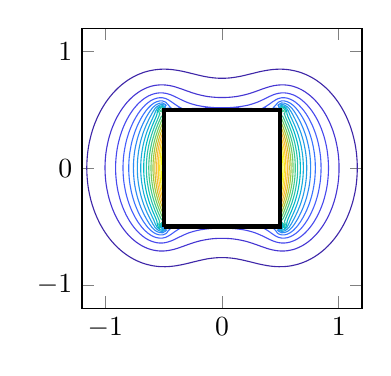
\begin{tikzpicture}

\begin{axis}[%
width=1.4in,
height=1.4in,
at={(0in,0in)},
scale only axis,
colormap={mymap}{[1pt] rgb(0pt)=(0.2422,0.1504,0.6603); rgb(1pt)=(0.25039,0.164995,0.707614); rgb(2pt)=(0.257771,0.181781,0.751138); rgb(3pt)=(0.264729,0.197757,0.795214); rgb(4pt)=(0.270648,0.214676,0.836371); rgb(5pt)=(0.275114,0.234238,0.870986); rgb(6pt)=(0.2783,0.255871,0.899071); rgb(7pt)=(0.280333,0.278233,0.9221); rgb(8pt)=(0.281338,0.300595,0.941376); rgb(9pt)=(0.281014,0.322757,0.957886); rgb(10pt)=(0.279467,0.344671,0.971676); rgb(11pt)=(0.275971,0.366681,0.982905); rgb(12pt)=(0.269914,0.3892,0.9906); rgb(13pt)=(0.260243,0.412329,0.995157); rgb(14pt)=(0.244033,0.435833,0.998833); rgb(15pt)=(0.220643,0.460257,0.997286); rgb(16pt)=(0.196333,0.484719,0.989152); rgb(17pt)=(0.183405,0.507371,0.979795); rgb(18pt)=(0.178643,0.528857,0.968157); rgb(19pt)=(0.176438,0.549905,0.952019); rgb(20pt)=(0.168743,0.570262,0.935871); rgb(21pt)=(0.154,0.5902,0.9218); rgb(22pt)=(0.146029,0.609119,0.907857); rgb(23pt)=(0.138024,0.627629,0.89729); rgb(24pt)=(0.124814,0.645929,0.888343); rgb(25pt)=(0.111252,0.6635,0.876314); rgb(26pt)=(0.0952095,0.679829,0.859781); rgb(27pt)=(0.0688714,0.694771,0.839357); rgb(28pt)=(0.0296667,0.708167,0.816333); rgb(29pt)=(0.00357143,0.720267,0.7917); rgb(30pt)=(0.00665714,0.731214,0.766014); rgb(31pt)=(0.0433286,0.741095,0.73941); rgb(32pt)=(0.0963952,0.75,0.712038); rgb(33pt)=(0.140771,0.7584,0.684157); rgb(34pt)=(0.1717,0.766962,0.655443); rgb(35pt)=(0.193767,0.775767,0.6251); rgb(36pt)=(0.216086,0.7843,0.5923); rgb(37pt)=(0.246957,0.791795,0.556743); rgb(38pt)=(0.290614,0.79729,0.518829); rgb(39pt)=(0.340643,0.8008,0.478857); rgb(40pt)=(0.3909,0.802871,0.435448); rgb(41pt)=(0.445629,0.802419,0.390919); rgb(42pt)=(0.5044,0.7993,0.348); rgb(43pt)=(0.561562,0.794233,0.304481); rgb(44pt)=(0.617395,0.787619,0.261238); rgb(45pt)=(0.671986,0.779271,0.2227); rgb(46pt)=(0.7242,0.769843,0.191029); rgb(47pt)=(0.773833,0.759805,0.16461); rgb(48pt)=(0.820314,0.749814,0.153529); rgb(49pt)=(0.863433,0.7406,0.159633); rgb(50pt)=(0.903543,0.733029,0.177414); rgb(51pt)=(0.939257,0.728786,0.209957); rgb(52pt)=(0.972757,0.729771,0.239443); rgb(53pt)=(0.995648,0.743371,0.237148); rgb(54pt)=(0.996986,0.765857,0.219943); rgb(55pt)=(0.995205,0.789252,0.202762); rgb(56pt)=(0.9892,0.813567,0.188533); rgb(57pt)=(0.978629,0.838629,0.176557); rgb(58pt)=(0.967648,0.8639,0.16429); rgb(59pt)=(0.96101,0.889019,0.153676); rgb(60pt)=(0.959671,0.913457,0.142257); rgb(61pt)=(0.962795,0.937338,0.12651); rgb(62pt)=(0.969114,0.960629,0.106362); rgb(63pt)=(0.9769,0.9839,0.0805)},
xmin=-1.2000,
xmax=1.2000,
ymin=-1.2000,
ymax=1.2000,
axis background/.style={fill=white}
]
\addplot[contour prepared, contour prepared format=matlab, contour/labels=false] table[row sep=crcr] {%
%
0.0526	337.0000\\
-1.1567	-0.0703\\
-1.1576	-0.0572\\
-1.1587	-0.0323\\
-1.1593	-0.0075\\
-1.1592	0.0174\\
-1.1586	0.0423\\
-1.1573	0.0672\\
-1.1567	0.0754\\
-1.1556	0.0920\\
-1.1534	0.1169\\
-1.1506	0.1418\\
-1.1472	0.1667\\
-1.1432	0.1915\\
-1.1385	0.2164\\
-1.1330	0.2413\\
-1.1318	0.2460\\
-1.1272	0.2662\\
-1.1208	0.2910\\
-1.1135	0.3159\\
-1.1070	0.3357\\
-1.1054	0.3408\\
-1.0970	0.3657\\
-1.0875	0.3905\\
-1.0821	0.4033\\
-1.0772	0.4154\\
-1.0663	0.4403\\
-1.0572	0.4587\\
-1.0542	0.4652\\
-1.0414	0.4900\\
-1.0323	0.5059\\
-1.0274	0.5149\\
-1.0123	0.5398\\
-1.0075	0.5471\\
-0.9961	0.5647\\
-0.9826	0.5835\\
-0.9783	0.5896\\
-0.9590	0.6144\\
-0.9577	0.6160\\
-0.9382	0.6393\\
-0.9328	0.6452\\
-0.9153	0.6642\\
-0.9080	0.6716\\
-0.8900	0.6891\\
-0.8831	0.6954\\
-0.8617	0.7139\\
-0.8582	0.7168\\
-0.8333	0.7363\\
-0.8298	0.7388\\
-0.8085	0.7539\\
-0.7930	0.7637\\
-0.7836	0.7696\\
-0.7587	0.7837\\
-0.7490	0.7886\\
-0.7338	0.7963\\
-0.7090	0.8073\\
-0.6926	0.8134\\
-0.6841	0.8168\\
-0.6592	0.8253\\
-0.6343	0.8322\\
-0.6095	0.8376\\
-0.6054	0.8383\\
-0.5846	0.8423\\
-0.5597	0.8457\\
-0.5348	0.8479\\
-0.5100	0.8490\\
-0.4851	0.8490\\
-0.4602	0.8480\\
-0.4353	0.8461\\
-0.4104	0.8431\\
-0.3856	0.8393\\
-0.3803	0.8383\\
-0.3607	0.8350\\
-0.3358	0.8301\\
-0.3109	0.8246\\
-0.2861	0.8186\\
-0.2660	0.8134\\
-0.2612	0.8123\\
-0.2363	0.8063\\
-0.2114	0.8002\\
-0.1866	0.7943\\
-0.1617	0.7886\\
-0.1613	0.7886\\
-0.1368	0.7839\\
-0.1119	0.7798\\
-0.0871	0.7763\\
-0.0622	0.7736\\
-0.0373	0.7718\\
-0.0124	0.7709\\
0.0124	0.7709\\
0.0373	0.7718\\
0.0622	0.7736\\
0.0871	0.7763\\
0.1119	0.7798\\
0.1368	0.7839\\
0.1613	0.7886\\
0.1617	0.7886\\
0.1866	0.7943\\
0.2114	0.8002\\
0.2363	0.8063\\
0.2612	0.8123\\
0.2660	0.8134\\
0.2861	0.8186\\
0.3109	0.8246\\
0.3358	0.8301\\
0.3607	0.8350\\
0.3803	0.8383\\
0.3856	0.8393\\
0.4104	0.8431\\
0.4353	0.8461\\
0.4602	0.8480\\
0.4851	0.8490\\
0.5100	0.8490\\
0.5348	0.8479\\
0.5597	0.8457\\
0.5846	0.8423\\
0.6054	0.8383\\
0.6095	0.8376\\
0.6343	0.8322\\
0.6592	0.8253\\
0.6841	0.8168\\
0.6926	0.8134\\
0.7090	0.8073\\
0.7338	0.7963\\
0.7490	0.7886\\
0.7587	0.7837\\
0.7836	0.7696\\
0.7930	0.7637\\
0.8085	0.7539\\
0.8298	0.7388\\
0.8333	0.7363\\
0.8582	0.7168\\
0.8617	0.7139\\
0.8831	0.6954\\
0.8900	0.6891\\
0.9080	0.6716\\
0.9153	0.6642\\
0.9328	0.6452\\
0.9382	0.6393\\
0.9577	0.6160\\
0.9590	0.6144\\
0.9783	0.5896\\
0.9826	0.5835\\
0.9961	0.5647\\
1.0075	0.5471\\
1.0123	0.5398\\
1.0274	0.5149\\
1.0323	0.5059\\
1.0414	0.4900\\
1.0542	0.4652\\
1.0572	0.4587\\
1.0663	0.4403\\
1.0772	0.4154\\
1.0821	0.4033\\
1.0875	0.3905\\
1.0970	0.3657\\
1.1054	0.3408\\
1.1070	0.3357\\
1.1135	0.3159\\
1.1208	0.2910\\
1.1272	0.2662\\
1.1318	0.2460\\
1.1330	0.2413\\
1.1385	0.2164\\
1.1432	0.1915\\
1.1472	0.1667\\
1.1506	0.1418\\
1.1534	0.1169\\
1.1556	0.0920\\
1.1567	0.0754\\
1.1573	0.0672\\
1.1586	0.0423\\
1.1592	0.0174\\
1.1593	-0.0075\\
1.1587	-0.0323\\
1.1576	-0.0572\\
1.1567	-0.0703\\
1.1560	-0.0821\\
1.1539	-0.1070\\
1.1512	-0.1318\\
1.1480	-0.1567\\
1.1441	-0.1816\\
1.1395	-0.2065\\
1.1342	-0.2313\\
1.1318	-0.2409\\
1.1284	-0.2562\\
1.1222	-0.2811\\
1.1150	-0.3060\\
1.1070	-0.3308\\
1.1070	-0.3309\\
1.0988	-0.3557\\
1.0895	-0.3806\\
1.0821	-0.3983\\
1.0793	-0.4055\\
1.0686	-0.4303\\
1.0572	-0.4537\\
1.0565	-0.4552\\
1.0441	-0.4801\\
1.0323	-0.5009\\
1.0301	-0.5050\\
1.0154	-0.5299\\
1.0075	-0.5421\\
0.9994	-0.5547\\
0.9826	-0.5785\\
0.9818	-0.5796\\
0.9631	-0.6045\\
0.9577	-0.6111\\
0.9426	-0.6294\\
0.9328	-0.6403\\
0.9201	-0.6542\\
0.9080	-0.6667\\
0.8953	-0.6791\\
0.8831	-0.6905\\
0.8677	-0.7040\\
0.8582	-0.7120\\
0.8365	-0.7289\\
0.8333	-0.7313\\
0.8085	-0.7489\\
0.8009	-0.7537\\
0.7836	-0.7647\\
0.7587	-0.7785\\
0.7585	-0.7786\\
0.7338	-0.7914\\
0.7090	-0.8021\\
0.7054	-0.8035\\
0.6841	-0.8120\\
0.6592	-0.8203\\
0.6343	-0.8270\\
0.6280	-0.8284\\
0.6095	-0.8328\\
0.5846	-0.8375\\
0.5597	-0.8408\\
0.5348	-0.8430\\
0.5100	-0.8440\\
0.4851	-0.8441\\
0.4602	-0.8431\\
0.4353	-0.8411\\
0.4104	-0.8383\\
0.3856	-0.8345\\
0.3607	-0.8299\\
0.3531	-0.8284\\
0.3358	-0.8250\\
0.3109	-0.8196\\
0.2861	-0.8137\\
0.2612	-0.8074\\
0.2459	-0.8035\\
0.2363	-0.8012\\
0.2114	-0.7952\\
0.1866	-0.7894\\
0.1617	-0.7839\\
0.1368	-0.7788\\
0.1359	-0.7786\\
0.1119	-0.7747\\
0.0871	-0.7713\\
0.0622	-0.7687\\
0.0373	-0.7669\\
0.0124	-0.7660\\
-0.0124	-0.7660\\
-0.0373	-0.7669\\
-0.0622	-0.7687\\
-0.0871	-0.7713\\
-0.1119	-0.7747\\
-0.1359	-0.7786\\
-0.1368	-0.7788\\
-0.1617	-0.7839\\
-0.1866	-0.7894\\
-0.2114	-0.7952\\
-0.2363	-0.8012\\
-0.2459	-0.8035\\
-0.2612	-0.8074\\
-0.2861	-0.8137\\
-0.3109	-0.8196\\
-0.3358	-0.8250\\
-0.3531	-0.8284\\
-0.3607	-0.8299\\
-0.3856	-0.8345\\
-0.4104	-0.8383\\
-0.4353	-0.8411\\
-0.4602	-0.8431\\
-0.4851	-0.8441\\
-0.5100	-0.8440\\
-0.5348	-0.8430\\
-0.5597	-0.8408\\
-0.5846	-0.8375\\
-0.6095	-0.8328\\
-0.6280	-0.8284\\
-0.6343	-0.8270\\
-0.6592	-0.8203\\
-0.6841	-0.8120\\
-0.7054	-0.8035\\
-0.7090	-0.8021\\
-0.7338	-0.7914\\
-0.7585	-0.7786\\
-0.7587	-0.7785\\
-0.7836	-0.7647\\
-0.8009	-0.7537\\
-0.8085	-0.7489\\
-0.8333	-0.7313\\
-0.8365	-0.7289\\
-0.8582	-0.7120\\
-0.8677	-0.7040\\
-0.8831	-0.6905\\
-0.8953	-0.6791\\
-0.9080	-0.6667\\
-0.9201	-0.6542\\
-0.9328	-0.6403\\
-0.9426	-0.6294\\
-0.9577	-0.6111\\
-0.9631	-0.6045\\
-0.9818	-0.5796\\
-0.9826	-0.5785\\
-0.9994	-0.5547\\
-1.0075	-0.5421\\
-1.0154	-0.5299\\
-1.0301	-0.5050\\
-1.0323	-0.5009\\
-1.0441	-0.4801\\
-1.0565	-0.4552\\
-1.0572	-0.4537\\
-1.0686	-0.4303\\
-1.0793	-0.4055\\
-1.0821	-0.3983\\
-1.0895	-0.3806\\
-1.0988	-0.3557\\
-1.1070	-0.3309\\
-1.1070	-0.3308\\
-1.1150	-0.3060\\
-1.1222	-0.2811\\
-1.1284	-0.2562\\
-1.1318	-0.2409\\
-1.1342	-0.2313\\
-1.1395	-0.2065\\
-1.1441	-0.1816\\
-1.1480	-0.1567\\
-1.1512	-0.1318\\
-1.1539	-0.1070\\
-1.1560	-0.0821\\
-1.1567	-0.0703\\
0.0526	161.0000\\
-0.4851	0.4947\\
-0.4873	0.4900\\
-0.4875	0.4652\\
-0.4872	0.4403\\
-0.4871	0.4154\\
-0.4870	0.3905\\
-0.4869	0.3657\\
-0.4868	0.3408\\
-0.4868	0.3159\\
-0.4867	0.2910\\
-0.4866	0.2662\\
-0.4866	0.2413\\
-0.4866	0.2164\\
-0.4865	0.1915\\
-0.4865	0.1667\\
-0.4865	0.1418\\
-0.4864	0.1169\\
-0.4864	0.0920\\
-0.4864	0.0672\\
-0.4864	0.0423\\
-0.4864	0.0174\\
-0.4864	-0.0075\\
-0.4864	-0.0323\\
-0.4864	-0.0572\\
-0.4864	-0.0821\\
-0.4864	-0.1070\\
-0.4864	-0.1318\\
-0.4865	-0.1567\\
-0.4865	-0.1816\\
-0.4865	-0.2065\\
-0.4866	-0.2313\\
-0.4866	-0.2562\\
-0.4867	-0.2811\\
-0.4868	-0.3060\\
-0.4868	-0.3308\\
-0.4869	-0.3557\\
-0.4870	-0.3806\\
-0.4871	-0.4055\\
-0.4872	-0.4303\\
-0.4874	-0.4552\\
-0.4884	-0.4801\\
-0.4851	-0.4869\\
-0.4602	-0.4848\\
-0.4353	-0.4850\\
-0.4104	-0.4854\\
-0.3856	-0.4857\\
-0.3607	-0.4861\\
-0.3358	-0.4864\\
-0.3109	-0.4866\\
-0.2861	-0.4869\\
-0.2612	-0.4871\\
-0.2363	-0.4873\\
-0.2114	-0.4874\\
-0.1866	-0.4876\\
-0.1617	-0.4877\\
-0.1368	-0.4878\\
-0.1119	-0.4879\\
-0.0871	-0.4880\\
-0.0622	-0.4880\\
-0.0373	-0.4881\\
-0.0124	-0.4881\\
0.0124	-0.4881\\
0.0373	-0.4881\\
0.0622	-0.4880\\
0.0871	-0.4880\\
0.1119	-0.4879\\
0.1368	-0.4878\\
0.1617	-0.4877\\
0.1866	-0.4876\\
0.2114	-0.4874\\
0.2363	-0.4873\\
0.2612	-0.4871\\
0.2861	-0.4869\\
0.3109	-0.4866\\
0.3358	-0.4864\\
0.3607	-0.4861\\
0.3856	-0.4857\\
0.4104	-0.4854\\
0.4353	-0.4850\\
0.4602	-0.4848\\
0.4851	-0.4869\\
0.4884	-0.4801\\
0.4874	-0.4552\\
0.4872	-0.4303\\
0.4871	-0.4055\\
0.4870	-0.3806\\
0.4869	-0.3557\\
0.4868	-0.3308\\
0.4868	-0.3060\\
0.4867	-0.2811\\
0.4866	-0.2562\\
0.4866	-0.2313\\
0.4865	-0.2065\\
0.4865	-0.1816\\
0.4865	-0.1567\\
0.4864	-0.1318\\
0.4864	-0.1070\\
0.4864	-0.0821\\
0.4864	-0.0572\\
0.4864	-0.0323\\
0.4864	-0.0075\\
0.4864	0.0174\\
0.4864	0.0423\\
0.4864	0.0672\\
0.4864	0.0920\\
0.4864	0.1169\\
0.4865	0.1418\\
0.4865	0.1667\\
0.4865	0.1915\\
0.4866	0.2164\\
0.4866	0.2413\\
0.4866	0.2662\\
0.4867	0.2910\\
0.4868	0.3159\\
0.4868	0.3408\\
0.4869	0.3657\\
0.4870	0.3905\\
0.4871	0.4154\\
0.4872	0.4403\\
0.4875	0.4652\\
0.4873	0.4900\\
0.4851	0.4947\\
0.4602	0.4948\\
0.4353	0.4950\\
0.4104	0.4954\\
0.3856	0.4958\\
0.3607	0.4961\\
0.3358	0.4964\\
0.3109	0.4967\\
0.2861	0.4969\\
0.2612	0.4972\\
0.2363	0.4974\\
0.2114	0.4975\\
0.1866	0.4977\\
0.1617	0.4978\\
0.1368	0.4979\\
0.1119	0.4980\\
0.0871	0.4981\\
0.0622	0.4982\\
0.0373	0.4982\\
0.0124	0.4982\\
-0.0124	0.4982\\
-0.0373	0.4982\\
-0.0622	0.4982\\
-0.0871	0.4981\\
-0.1119	0.4980\\
-0.1368	0.4979\\
-0.1617	0.4978\\
-0.1866	0.4977\\
-0.2114	0.4975\\
-0.2363	0.4974\\
-0.2612	0.4972\\
-0.2861	0.4969\\
-0.3109	0.4967\\
-0.3358	0.4964\\
-0.3607	0.4961\\
-0.3856	0.4958\\
-0.4104	0.4954\\
-0.4353	0.4950\\
-0.4602	0.4948\\
-0.4851	0.4947\\
0.1053	297.0000\\
-0.9826	-0.1979\\
-0.9860	-0.1816\\
-0.9904	-0.1567\\
-0.9942	-0.1318\\
-0.9972	-0.1070\\
-0.9995	-0.0821\\
-1.0013	-0.0572\\
-1.0024	-0.0323\\
-1.0029	-0.0075\\
-1.0029	0.0174\\
-1.0022	0.0423\\
-1.0010	0.0672\\
-0.9991	0.0920\\
-0.9966	0.1169\\
-0.9935	0.1418\\
-0.9896	0.1667\\
-0.9850	0.1915\\
-0.9826	0.2029\\
-0.9799	0.2164\\
-0.9743	0.2413\\
-0.9678	0.2662\\
-0.9603	0.2910\\
-0.9577	0.2988\\
-0.9524	0.3159\\
-0.9436	0.3408\\
-0.9336	0.3657\\
-0.9328	0.3674\\
-0.9232	0.3905\\
-0.9114	0.4154\\
-0.9080	0.4220\\
-0.8988	0.4403\\
-0.8847	0.4652\\
-0.8831	0.4677\\
-0.8697	0.4900\\
-0.8582	0.5069\\
-0.8528	0.5149\\
-0.8342	0.5398\\
-0.8333	0.5408\\
-0.8138	0.5647\\
-0.8085	0.5706\\
-0.7908	0.5896\\
-0.7836	0.5966\\
-0.7644	0.6144\\
-0.7587	0.6194\\
-0.7338	0.6391\\
-0.7335	0.6393\\
-0.7090	0.6565\\
-0.6961	0.6642\\
-0.6841	0.6712\\
-0.6592	0.6836\\
-0.6456	0.6891\\
-0.6343	0.6938\\
-0.6095	0.7021\\
-0.5846	0.7081\\
-0.5597	0.7120\\
-0.5368	0.7139\\
-0.5348	0.7141\\
-0.5100	0.7146\\
-0.4991	0.7139\\
-0.4851	0.7132\\
-0.4602	0.7103\\
-0.4353	0.7058\\
-0.4104	0.6998\\
-0.3856	0.6923\\
-0.3759	0.6891\\
-0.3607	0.6841\\
-0.3358	0.6754\\
-0.3109	0.6661\\
-0.3056	0.6642\\
-0.2861	0.6573\\
-0.2612	0.6488\\
-0.2363	0.6406\\
-0.2322	0.6393\\
-0.2114	0.6335\\
-0.1866	0.6272\\
-0.1617	0.6217\\
-0.1368	0.6169\\
-0.1217	0.6144\\
-0.1119	0.6130\\
-0.0871	0.6102\\
-0.0622	0.6081\\
-0.0373	0.6066\\
-0.0124	0.6059\\
0.0124	0.6059\\
0.0373	0.6066\\
0.0622	0.6081\\
0.0871	0.6102\\
0.1119	0.6130\\
0.1217	0.6144\\
0.1368	0.6169\\
0.1617	0.6217\\
0.1866	0.6272\\
0.2114	0.6335\\
0.2322	0.6393\\
0.2363	0.6406\\
0.2612	0.6488\\
0.2861	0.6573\\
0.3056	0.6642\\
0.3109	0.6661\\
0.3358	0.6754\\
0.3607	0.6841\\
0.3759	0.6891\\
0.3856	0.6923\\
0.4104	0.6998\\
0.4353	0.7058\\
0.4602	0.7103\\
0.4851	0.7132\\
0.4991	0.7139\\
0.5100	0.7146\\
0.5348	0.7141\\
0.5368	0.7139\\
0.5597	0.7120\\
0.5846	0.7081\\
0.6095	0.7021\\
0.6343	0.6938\\
0.6456	0.6891\\
0.6592	0.6836\\
0.6841	0.6712\\
0.6961	0.6642\\
0.7090	0.6565\\
0.7335	0.6393\\
0.7338	0.6391\\
0.7587	0.6194\\
0.7644	0.6144\\
0.7836	0.5966\\
0.7908	0.5896\\
0.8085	0.5706\\
0.8138	0.5647\\
0.8333	0.5408\\
0.8342	0.5398\\
0.8528	0.5149\\
0.8582	0.5069\\
0.8697	0.4900\\
0.8831	0.4677\\
0.8847	0.4652\\
0.8988	0.4403\\
0.9080	0.4220\\
0.9114	0.4154\\
0.9232	0.3905\\
0.9328	0.3674\\
0.9336	0.3657\\
0.9436	0.3408\\
0.9524	0.3159\\
0.9577	0.2988\\
0.9603	0.2910\\
0.9678	0.2662\\
0.9743	0.2413\\
0.9799	0.2164\\
0.9826	0.2029\\
0.9850	0.1915\\
0.9896	0.1667\\
0.9935	0.1418\\
0.9966	0.1169\\
0.9991	0.0920\\
1.0010	0.0672\\
1.0022	0.0423\\
1.0029	0.0174\\
1.0029	-0.0075\\
1.0024	-0.0323\\
1.0013	-0.0572\\
0.9995	-0.0821\\
0.9972	-0.1070\\
0.9942	-0.1318\\
0.9904	-0.1567\\
0.9860	-0.1816\\
0.9826	-0.1979\\
0.9809	-0.2065\\
0.9755	-0.2313\\
0.9692	-0.2562\\
0.9619	-0.2811\\
0.9577	-0.2938\\
0.9540	-0.3060\\
0.9455	-0.3308\\
0.9357	-0.3557\\
0.9328	-0.3623\\
0.9254	-0.3806\\
0.9139	-0.4055\\
0.9080	-0.4170\\
0.9014	-0.4303\\
0.8877	-0.4552\\
0.8831	-0.4628\\
0.8728	-0.4801\\
0.8582	-0.5019\\
0.8562	-0.5050\\
0.8382	-0.5299\\
0.8333	-0.5359\\
0.8182	-0.5547\\
0.8085	-0.5656\\
0.7957	-0.5796\\
0.7836	-0.5917\\
0.7700	-0.6045\\
0.7587	-0.6145\\
0.7402	-0.6294\\
0.7338	-0.6343\\
0.7090	-0.6514\\
0.7043	-0.6542\\
0.6841	-0.6663\\
0.6592	-0.6784\\
0.6575	-0.6791\\
0.6343	-0.6890\\
0.6095	-0.6970\\
0.5846	-0.7028\\
0.5772	-0.7040\\
0.5597	-0.7071\\
0.5348	-0.7095\\
0.5100	-0.7099\\
0.4851	-0.7085\\
0.4602	-0.7052\\
0.4539	-0.7040\\
0.4353	-0.7007\\
0.4104	-0.6948\\
0.3856	-0.6875\\
0.3611	-0.6791\\
0.3607	-0.6790\\
0.3358	-0.6704\\
0.3109	-0.6613\\
0.2918	-0.6542\\
0.2861	-0.6522\\
0.2612	-0.6438\\
0.2363	-0.6358\\
0.2150	-0.6294\\
0.2114	-0.6284\\
0.1866	-0.6222\\
0.1617	-0.6168\\
0.1368	-0.6121\\
0.1119	-0.6082\\
0.0871	-0.6050\\
0.0815	-0.6045\\
0.0622	-0.6029\\
0.0373	-0.6015\\
0.0124	-0.6008\\
-0.0124	-0.6008\\
-0.0373	-0.6015\\
-0.0622	-0.6029\\
-0.0815	-0.6045\\
-0.0871	-0.6050\\
-0.1119	-0.6082\\
-0.1368	-0.6121\\
-0.1617	-0.6168\\
-0.1866	-0.6222\\
-0.2114	-0.6284\\
-0.2150	-0.6294\\
-0.2363	-0.6358\\
-0.2612	-0.6438\\
-0.2861	-0.6522\\
-0.2918	-0.6542\\
-0.3109	-0.6613\\
-0.3358	-0.6704\\
-0.3607	-0.6790\\
-0.3611	-0.6791\\
-0.3856	-0.6875\\
-0.4104	-0.6948\\
-0.4353	-0.7007\\
-0.4539	-0.7040\\
-0.4602	-0.7052\\
-0.4851	-0.7085\\
-0.5100	-0.7099\\
-0.5348	-0.7095\\
-0.5597	-0.7071\\
-0.5772	-0.7040\\
-0.5846	-0.7028\\
-0.6095	-0.6970\\
-0.6343	-0.6890\\
-0.6575	-0.6791\\
-0.6592	-0.6784\\
-0.6841	-0.6663\\
-0.7043	-0.6542\\
-0.7090	-0.6514\\
-0.7338	-0.6343\\
-0.7402	-0.6294\\
-0.7587	-0.6145\\
-0.7700	-0.6045\\
-0.7836	-0.5917\\
-0.7957	-0.5796\\
-0.8085	-0.5656\\
-0.8182	-0.5547\\
-0.8333	-0.5359\\
-0.8382	-0.5299\\
-0.8562	-0.5050\\
-0.8582	-0.5019\\
-0.8728	-0.4801\\
-0.8831	-0.4628\\
-0.8877	-0.4552\\
-0.9014	-0.4303\\
-0.9080	-0.4170\\
-0.9139	-0.4055\\
-0.9254	-0.3806\\
-0.9328	-0.3623\\
-0.9357	-0.3557\\
-0.9455	-0.3308\\
-0.9540	-0.3060\\
-0.9577	-0.2938\\
-0.9619	-0.2811\\
-0.9692	-0.2562\\
-0.9755	-0.2313\\
-0.9809	-0.2065\\
-0.9826	-0.1979\\
0.1053	161.0000\\
-0.4851	0.4993\\
-0.4895	0.4900\\
-0.4899	0.4652\\
-0.4894	0.4403\\
-0.4891	0.4154\\
-0.4889	0.3905\\
-0.4888	0.3657\\
-0.4886	0.3408\\
-0.4885	0.3159\\
-0.4883	0.2910\\
-0.4882	0.2662\\
-0.4881	0.2413\\
-0.4880	0.2164\\
-0.4880	0.1915\\
-0.4879	0.1667\\
-0.4878	0.1418\\
-0.4878	0.1169\\
-0.4877	0.0920\\
-0.4877	0.0672\\
-0.4877	0.0423\\
-0.4877	0.0174\\
-0.4877	-0.0075\\
-0.4877	-0.0323\\
-0.4877	-0.0572\\
-0.4877	-0.0821\\
-0.4878	-0.1070\\
-0.4878	-0.1318\\
-0.4879	-0.1567\\
-0.4879	-0.1816\\
-0.4880	-0.2065\\
-0.4881	-0.2313\\
-0.4882	-0.2562\\
-0.4883	-0.2811\\
-0.4884	-0.3060\\
-0.4886	-0.3308\\
-0.4887	-0.3557\\
-0.4889	-0.3806\\
-0.4891	-0.4055\\
-0.4893	-0.4303\\
-0.4897	-0.4552\\
-0.4918	-0.4801\\
-0.4851	-0.4937\\
-0.4602	-0.4894\\
-0.4353	-0.4899\\
-0.4104	-0.4906\\
-0.3856	-0.4914\\
-0.3607	-0.4920\\
-0.3358	-0.4926\\
-0.3109	-0.4931\\
-0.2861	-0.4936\\
-0.2612	-0.4940\\
-0.2363	-0.4944\\
-0.2114	-0.4948\\
-0.1866	-0.4950\\
-0.1617	-0.4953\\
-0.1368	-0.4955\\
-0.1119	-0.4957\\
-0.0871	-0.4958\\
-0.0622	-0.4960\\
-0.0373	-0.4960\\
-0.0124	-0.4961\\
0.0124	-0.4961\\
0.0373	-0.4960\\
0.0622	-0.4960\\
0.0871	-0.4958\\
0.1119	-0.4957\\
0.1368	-0.4955\\
0.1617	-0.4953\\
0.1866	-0.4950\\
0.2114	-0.4948\\
0.2363	-0.4944\\
0.2612	-0.4940\\
0.2861	-0.4936\\
0.3109	-0.4931\\
0.3358	-0.4926\\
0.3607	-0.4920\\
0.3856	-0.4914\\
0.4104	-0.4906\\
0.4353	-0.4899\\
0.4602	-0.4894\\
0.4851	-0.4937\\
0.4918	-0.4801\\
0.4897	-0.4552\\
0.4893	-0.4303\\
0.4891	-0.4055\\
0.4889	-0.3806\\
0.4887	-0.3557\\
0.4886	-0.3308\\
0.4884	-0.3060\\
0.4883	-0.2811\\
0.4882	-0.2562\\
0.4881	-0.2313\\
0.4880	-0.2065\\
0.4879	-0.1816\\
0.4879	-0.1567\\
0.4878	-0.1318\\
0.4878	-0.1070\\
0.4877	-0.0821\\
0.4877	-0.0572\\
0.4877	-0.0323\\
0.4877	-0.0075\\
0.4877	0.0174\\
0.4877	0.0423\\
0.4877	0.0672\\
0.4877	0.0920\\
0.4878	0.1169\\
0.4878	0.1418\\
0.4879	0.1667\\
0.4880	0.1915\\
0.4880	0.2164\\
0.4881	0.2413\\
0.4882	0.2662\\
0.4883	0.2910\\
0.4885	0.3159\\
0.4886	0.3408\\
0.4888	0.3657\\
0.4889	0.3905\\
0.4891	0.4154\\
0.4894	0.4403\\
0.4899	0.4652\\
0.4895	0.4900\\
0.4851	0.4993\\
0.4602	0.4995\\
0.4353	0.5000\\
0.4104	0.5008\\
0.3856	0.5015\\
0.3607	0.5022\\
0.3358	0.5028\\
0.3109	0.5034\\
0.2861	0.5038\\
0.2612	0.5043\\
0.2363	0.5047\\
0.2114	0.5050\\
0.1866	0.5053\\
0.1617	0.5056\\
0.1368	0.5058\\
0.1119	0.5060\\
0.0871	0.5062\\
0.0622	0.5063\\
0.0373	0.5064\\
0.0124	0.5064\\
-0.0124	0.5064\\
-0.0373	0.5064\\
-0.0622	0.5063\\
-0.0871	0.5062\\
-0.1119	0.5060\\
-0.1368	0.5058\\
-0.1617	0.5056\\
-0.1866	0.5053\\
-0.2114	0.5050\\
-0.2363	0.5047\\
-0.2612	0.5043\\
-0.2861	0.5038\\
-0.3109	0.5034\\
-0.3358	0.5028\\
-0.3607	0.5022\\
-0.3856	0.5015\\
-0.4104	0.5008\\
-0.4353	0.5000\\
-0.4602	0.4995\\
-0.4851	0.4993\\
0.1579	273.0000\\
-0.9080	-0.0881\\
-0.9086	-0.0821\\
-0.9105	-0.0572\\
-0.9118	-0.0323\\
-0.9124	-0.0075\\
-0.9123	0.0174\\
-0.9116	0.0423\\
-0.9102	0.0672\\
-0.9081	0.0920\\
-0.9080	0.0935\\
-0.9056	0.1169\\
-0.9025	0.1418\\
-0.8986	0.1667\\
-0.8940	0.1915\\
-0.8886	0.2164\\
-0.8831	0.2380\\
-0.8823	0.2413\\
-0.8758	0.2662\\
-0.8682	0.2910\\
-0.8595	0.3159\\
-0.8582	0.3192\\
-0.8504	0.3408\\
-0.8401	0.3657\\
-0.8333	0.3802\\
-0.8288	0.3905\\
-0.8165	0.4154\\
-0.8085	0.4297\\
-0.8028	0.4403\\
-0.7877	0.4652\\
-0.7836	0.4712\\
-0.7711	0.4900\\
-0.7587	0.5065\\
-0.7524	0.5149\\
-0.7338	0.5367\\
-0.7311	0.5398\\
-0.7090	0.5624\\
-0.7066	0.5647\\
-0.6841	0.5843\\
-0.6774	0.5896\\
-0.6592	0.6026\\
-0.6393	0.6144\\
-0.6343	0.6173\\
-0.6095	0.6292\\
-0.5846	0.6374\\
-0.5757	0.6393\\
-0.5597	0.6431\\
-0.5348	0.6460\\
-0.5100	0.6457\\
-0.4851	0.6423\\
-0.4730	0.6393\\
-0.4602	0.6363\\
-0.4353	0.6278\\
-0.4104	0.6168\\
-0.4053	0.6144\\
-0.3856	0.6049\\
-0.3607	0.5924\\
-0.3548	0.5896\\
-0.3358	0.5805\\
-0.3109	0.5695\\
-0.2990	0.5647\\
-0.2861	0.5598\\
-0.2612	0.5515\\
-0.2363	0.5442\\
-0.2190	0.5398\\
-0.2114	0.5381\\
-0.1866	0.5333\\
-0.1617	0.5293\\
-0.1368	0.5260\\
-0.1119	0.5233\\
-0.0871	0.5211\\
-0.0622	0.5196\\
-0.0373	0.5186\\
-0.0124	0.5181\\
0.0124	0.5181\\
0.0373	0.5186\\
0.0622	0.5196\\
0.0871	0.5211\\
0.1119	0.5233\\
0.1368	0.5260\\
0.1617	0.5293\\
0.1866	0.5333\\
0.2114	0.5381\\
0.2190	0.5398\\
0.2363	0.5442\\
0.2612	0.5515\\
0.2861	0.5598\\
0.2990	0.5647\\
0.3109	0.5695\\
0.3358	0.5805\\
0.3548	0.5896\\
0.3607	0.5924\\
0.3856	0.6049\\
0.4053	0.6144\\
0.4104	0.6168\\
0.4353	0.6278\\
0.4602	0.6363\\
0.4730	0.6393\\
0.4851	0.6423\\
0.5100	0.6457\\
0.5348	0.6460\\
0.5597	0.6431\\
0.5757	0.6393\\
0.5846	0.6374\\
0.6095	0.6292\\
0.6343	0.6173\\
0.6393	0.6144\\
0.6592	0.6026\\
0.6774	0.5896\\
0.6841	0.5843\\
0.7066	0.5647\\
0.7090	0.5624\\
0.7311	0.5398\\
0.7338	0.5367\\
0.7524	0.5149\\
0.7587	0.5065\\
0.7711	0.4900\\
0.7836	0.4712\\
0.7877	0.4652\\
0.8028	0.4403\\
0.8085	0.4297\\
0.8165	0.4154\\
0.8288	0.3905\\
0.8333	0.3802\\
0.8401	0.3657\\
0.8504	0.3408\\
0.8582	0.3192\\
0.8595	0.3159\\
0.8682	0.2910\\
0.8758	0.2662\\
0.8823	0.2413\\
0.8831	0.2380\\
0.8886	0.2164\\
0.8940	0.1915\\
0.8986	0.1667\\
0.9025	0.1418\\
0.9056	0.1169\\
0.9080	0.0935\\
0.9081	0.0920\\
0.9102	0.0672\\
0.9116	0.0423\\
0.9123	0.0174\\
0.9124	-0.0075\\
0.9118	-0.0323\\
0.9105	-0.0572\\
0.9086	-0.0821\\
0.9080	-0.0881\\
0.9062	-0.1070\\
0.9032	-0.1318\\
0.8994	-0.1567\\
0.8950	-0.1816\\
0.8897	-0.2065\\
0.8836	-0.2313\\
0.8831	-0.2331\\
0.8771	-0.2562\\
0.8698	-0.2811\\
0.8613	-0.3060\\
0.8582	-0.3142\\
0.8523	-0.3308\\
0.8423	-0.3557\\
0.8333	-0.3752\\
0.8310	-0.3806\\
0.8191	-0.4055\\
0.8085	-0.4247\\
0.8055	-0.4303\\
0.7909	-0.4552\\
0.7836	-0.4662\\
0.7746	-0.4801\\
0.7587	-0.5015\\
0.7562	-0.5050\\
0.7355	-0.5299\\
0.7338	-0.5317\\
0.7119	-0.5547\\
0.7090	-0.5575\\
0.6841	-0.5792\\
0.6836	-0.5796\\
0.6592	-0.5976\\
0.6479	-0.6045\\
0.6343	-0.6125\\
0.6095	-0.6241\\
0.5935	-0.6294\\
0.5846	-0.6325\\
0.5597	-0.6384\\
0.5348	-0.6412\\
0.5100	-0.6410\\
0.4851	-0.6377\\
0.4602	-0.6313\\
0.4547	-0.6294\\
0.4353	-0.6228\\
0.4104	-0.6120\\
0.3949	-0.6045\\
0.3856	-0.5998\\
0.3607	-0.5875\\
0.3444	-0.5796\\
0.3358	-0.5755\\
0.3109	-0.5646\\
0.2864	-0.5547\\
0.2861	-0.5546\\
0.2612	-0.5465\\
0.2363	-0.5394\\
0.2114	-0.5332\\
0.1957	-0.5299\\
0.1866	-0.5281\\
0.1617	-0.5242\\
0.1368	-0.5210\\
0.1119	-0.5183\\
0.0871	-0.5163\\
0.0622	-0.5148\\
0.0373	-0.5138\\
0.0124	-0.5133\\
-0.0124	-0.5133\\
-0.0373	-0.5138\\
-0.0622	-0.5148\\
-0.0871	-0.5163\\
-0.1119	-0.5183\\
-0.1368	-0.5210\\
-0.1617	-0.5242\\
-0.1866	-0.5281\\
-0.1957	-0.5299\\
-0.2114	-0.5332\\
-0.2363	-0.5394\\
-0.2612	-0.5465\\
-0.2861	-0.5546\\
-0.2864	-0.5547\\
-0.3109	-0.5646\\
-0.3358	-0.5755\\
-0.3444	-0.5796\\
-0.3607	-0.5875\\
-0.3856	-0.5998\\
-0.3949	-0.6045\\
-0.4104	-0.6120\\
-0.4353	-0.6228\\
-0.4547	-0.6294\\
-0.4602	-0.6313\\
-0.4851	-0.6377\\
-0.5100	-0.6410\\
-0.5348	-0.6412\\
-0.5597	-0.6384\\
-0.5846	-0.6325\\
-0.5935	-0.6294\\
-0.6095	-0.6241\\
-0.6343	-0.6125\\
-0.6479	-0.6045\\
-0.6592	-0.5976\\
-0.6836	-0.5796\\
-0.6841	-0.5792\\
-0.7090	-0.5575\\
-0.7119	-0.5547\\
-0.7338	-0.5317\\
-0.7355	-0.5299\\
-0.7562	-0.5050\\
-0.7587	-0.5015\\
-0.7746	-0.4801\\
-0.7836	-0.4662\\
-0.7909	-0.4552\\
-0.8055	-0.4303\\
-0.8085	-0.4247\\
-0.8191	-0.4055\\
-0.8310	-0.3806\\
-0.8333	-0.3752\\
-0.8423	-0.3557\\
-0.8523	-0.3308\\
-0.8582	-0.3142\\
-0.8613	-0.3060\\
-0.8698	-0.2811\\
-0.8771	-0.2562\\
-0.8831	-0.2331\\
-0.8836	-0.2313\\
-0.8897	-0.2065\\
-0.8950	-0.1816\\
-0.8994	-0.1567\\
-0.9032	-0.1318\\
-0.9062	-0.1070\\
-0.9080	-0.0881\\
0.1579	161.0000\\
-0.4851	0.5040\\
-0.4917	0.4900\\
-0.4923	0.4652\\
-0.4915	0.4403\\
-0.4912	0.4154\\
-0.4909	0.3905\\
-0.4906	0.3657\\
-0.4904	0.3408\\
-0.4902	0.3159\\
-0.4900	0.2910\\
-0.4898	0.2662\\
-0.4896	0.2413\\
-0.4895	0.2164\\
-0.4894	0.1915\\
-0.4893	0.1667\\
-0.4892	0.1418\\
-0.4891	0.1169\\
-0.4891	0.0920\\
-0.4890	0.0672\\
-0.4890	0.0423\\
-0.4890	0.0174\\
-0.4890	-0.0075\\
-0.4890	-0.0323\\
-0.4890	-0.0572\\
-0.4891	-0.0821\\
-0.4891	-0.1070\\
-0.4892	-0.1318\\
-0.4893	-0.1567\\
-0.4894	-0.1816\\
-0.4895	-0.2065\\
-0.4896	-0.2313\\
-0.4898	-0.2562\\
-0.4899	-0.2811\\
-0.4901	-0.3060\\
-0.4903	-0.3308\\
-0.4906	-0.3557\\
-0.4908	-0.3806\\
-0.4911	-0.4055\\
-0.4914	-0.4303\\
-0.4921	-0.4552\\
-0.4951	-0.4801\\
-0.4851	-0.5004\\
-0.4602	-0.4941\\
-0.4353	-0.4948\\
-0.4104	-0.4959\\
-0.3856	-0.4970\\
-0.3607	-0.4980\\
-0.3358	-0.4989\\
-0.3109	-0.4997\\
-0.2861	-0.5004\\
-0.2612	-0.5010\\
-0.2363	-0.5016\\
-0.2114	-0.5021\\
-0.1866	-0.5025\\
-0.1617	-0.5029\\
-0.1368	-0.5032\\
-0.1119	-0.5035\\
-0.0871	-0.5037\\
-0.0622	-0.5039\\
-0.0373	-0.5040\\
-0.0124	-0.5040\\
0.0124	-0.5040\\
0.0373	-0.5040\\
0.0622	-0.5039\\
0.0871	-0.5037\\
0.1119	-0.5035\\
0.1368	-0.5032\\
0.1617	-0.5029\\
0.1866	-0.5025\\
0.2114	-0.5021\\
0.2363	-0.5016\\
0.2612	-0.5010\\
0.2861	-0.5004\\
0.3109	-0.4997\\
0.3358	-0.4989\\
0.3607	-0.4980\\
0.3856	-0.4970\\
0.4104	-0.4959\\
0.4353	-0.4948\\
0.4602	-0.4941\\
0.4851	-0.5004\\
0.4951	-0.4801\\
0.4921	-0.4552\\
0.4914	-0.4303\\
0.4911	-0.4055\\
0.4908	-0.3806\\
0.4906	-0.3557\\
0.4903	-0.3308\\
0.4901	-0.3060\\
0.4899	-0.2811\\
0.4898	-0.2562\\
0.4896	-0.2313\\
0.4895	-0.2065\\
0.4894	-0.1816\\
0.4893	-0.1567\\
0.4892	-0.1318\\
0.4891	-0.1070\\
0.4891	-0.0821\\
0.4890	-0.0572\\
0.4890	-0.0323\\
0.4890	-0.0075\\
0.4890	0.0174\\
0.4890	0.0423\\
0.4890	0.0672\\
0.4891	0.0920\\
0.4891	0.1169\\
0.4892	0.1418\\
0.4893	0.1667\\
0.4894	0.1915\\
0.4895	0.2164\\
0.4896	0.2413\\
0.4898	0.2662\\
0.4900	0.2910\\
0.4902	0.3159\\
0.4904	0.3408\\
0.4906	0.3657\\
0.4909	0.3905\\
0.4912	0.4154\\
0.4915	0.4403\\
0.4923	0.4652\\
0.4917	0.4900\\
0.4851	0.5040\\
0.4602	0.5043\\
0.4353	0.5050\\
0.4104	0.5062\\
0.3856	0.5073\\
0.3607	0.5083\\
0.3358	0.5092\\
0.3109	0.5100\\
0.2861	0.5107\\
0.2612	0.5114\\
0.2363	0.5120\\
0.2114	0.5125\\
0.1866	0.5130\\
0.1617	0.5134\\
0.1368	0.5137\\
0.1119	0.5140\\
0.0871	0.5142\\
0.0622	0.5144\\
0.0373	0.5145\\
0.0124	0.5146\\
-0.0124	0.5146\\
-0.0373	0.5145\\
-0.0622	0.5144\\
-0.0871	0.5142\\
-0.1119	0.5140\\
-0.1368	0.5137\\
-0.1617	0.5134\\
-0.1866	0.5130\\
-0.2114	0.5125\\
-0.2363	0.5120\\
-0.2612	0.5114\\
-0.2861	0.5107\\
-0.3109	0.5100\\
-0.3358	0.5092\\
-0.3607	0.5083\\
-0.3856	0.5073\\
-0.4104	0.5062\\
-0.4353	0.5050\\
-0.4602	0.5043\\
-0.4851	0.5040\\
0.2105	151.0000\\
-0.8333	-0.1666\\
-0.8352	-0.1567\\
-0.8393	-0.1318\\
-0.8426	-0.1070\\
-0.8451	-0.0821\\
-0.8470	-0.0572\\
-0.8482	-0.0323\\
-0.8488	-0.0075\\
-0.8487	0.0174\\
-0.8480	0.0423\\
-0.8467	0.0672\\
-0.8447	0.0920\\
-0.8420	0.1169\\
-0.8385	0.1418\\
-0.8343	0.1667\\
-0.8333	0.1717\\
-0.8297	0.1915\\
-0.8244	0.2164\\
-0.8183	0.2413\\
-0.8111	0.2662\\
-0.8085	0.2743\\
-0.8034	0.2910\\
-0.7949	0.3159\\
-0.7851	0.3408\\
-0.7836	0.3444\\
-0.7749	0.3657\\
-0.7632	0.3905\\
-0.7587	0.3992\\
-0.7506	0.4154\\
-0.7364	0.4403\\
-0.7338	0.4443\\
-0.7211	0.4652\\
-0.7090	0.4822\\
-0.7036	0.4900\\
-0.6841	0.5141\\
-0.6835	0.5149\\
-0.6602	0.5398\\
-0.6592	0.5407\\
-0.6343	0.5623\\
-0.6313	0.5647\\
-0.6095	0.5795\\
-0.5890	0.5896\\
-0.5846	0.5917\\
-0.5597	0.6004\\
-0.5348	0.6043\\
-0.5100	0.6038\\
-0.4851	0.5980\\
-0.4664	0.5896\\
-0.4602	0.5864\\
-0.4353	0.5703\\
-0.4268	0.5647\\
-0.4104	0.5525\\
-0.3914	0.5398\\
-0.3856	0.5358\\
-0.3607	0.5211\\
-0.3487	0.5149\\
-0.3607	0.5144\\
-0.3856	0.5130\\
-0.4104	0.5115\\
-0.4353	0.5100\\
-0.4602	0.5090\\
-0.4851	0.5086\\
-0.4939	0.4900\\
-0.4947	0.4652\\
-0.4937	0.4403\\
-0.4932	0.4154\\
-0.4928	0.3905\\
-0.4925	0.3657\\
-0.4921	0.3408\\
-0.4919	0.3159\\
-0.4916	0.2910\\
-0.4914	0.2662\\
-0.4912	0.2413\\
-0.4910	0.2164\\
-0.4908	0.1915\\
-0.4907	0.1667\\
-0.4906	0.1418\\
-0.4905	0.1169\\
-0.4904	0.0920\\
-0.4904	0.0672\\
-0.4903	0.0423\\
-0.4903	0.0174\\
-0.4903	-0.0075\\
-0.4903	-0.0323\\
-0.4904	-0.0572\\
-0.4904	-0.0821\\
-0.4905	-0.1070\\
-0.4906	-0.1318\\
-0.4907	-0.1567\\
-0.4908	-0.1816\\
-0.4910	-0.2065\\
-0.4911	-0.2313\\
-0.4913	-0.2562\\
-0.4916	-0.2811\\
-0.4918	-0.3060\\
-0.4921	-0.3308\\
-0.4924	-0.3557\\
-0.4927	-0.3806\\
-0.4931	-0.4055\\
-0.4935	-0.4303\\
-0.4944	-0.4552\\
-0.4984	-0.4801\\
-0.4884	-0.5050\\
-0.4851	-0.5079\\
-0.4802	-0.5050\\
-0.4602	-0.4987\\
-0.4353	-0.4996\\
-0.4104	-0.5012\\
-0.3856	-0.5026\\
-0.3607	-0.5039\\
-0.3388	-0.5050\\
-0.3607	-0.5162\\
-0.3840	-0.5299\\
-0.3856	-0.5308\\
-0.4104	-0.5476\\
-0.4199	-0.5547\\
-0.4353	-0.5653\\
-0.4569	-0.5796\\
-0.4602	-0.5815\\
-0.4851	-0.5931\\
-0.5100	-0.5986\\
-0.5348	-0.5991\\
-0.5597	-0.5954\\
-0.5846	-0.5870\\
-0.5994	-0.5796\\
-0.6095	-0.5744\\
-0.6343	-0.5574\\
-0.6377	-0.5547\\
-0.6592	-0.5358\\
-0.6654	-0.5299\\
-0.6841	-0.5092\\
-0.6878	-0.5050\\
-0.7070	-0.4801\\
-0.7090	-0.4773\\
-0.7243	-0.4552\\
-0.7338	-0.4393\\
-0.7395	-0.4303\\
-0.7532	-0.4055\\
-0.7587	-0.3942\\
-0.7657	-0.3806\\
-0.7770	-0.3557\\
-0.7836	-0.3393\\
-0.7872	-0.3308\\
-0.7967	-0.3060\\
-0.8050	-0.2811\\
-0.8085	-0.2693\\
-0.8126	-0.2562\\
-0.8196	-0.2313\\
-0.8256	-0.2065\\
-0.8307	-0.1816\\
-0.8333	-0.1666\\
0.2105	151.0000\\
0.3607	-0.5162\\
0.3388	-0.5050\\
0.3607	-0.5039\\
0.3856	-0.5026\\
0.4104	-0.5012\\
0.4353	-0.4996\\
0.4602	-0.4987\\
0.4802	-0.5050\\
0.4851	-0.5079\\
0.4884	-0.5050\\
0.4984	-0.4801\\
0.4944	-0.4552\\
0.4935	-0.4303\\
0.4931	-0.4055\\
0.4927	-0.3806\\
0.4924	-0.3557\\
0.4921	-0.3308\\
0.4918	-0.3060\\
0.4916	-0.2811\\
0.4913	-0.2562\\
0.4911	-0.2313\\
0.4910	-0.2065\\
0.4908	-0.1816\\
0.4907	-0.1567\\
0.4906	-0.1318\\
0.4905	-0.1070\\
0.4904	-0.0821\\
0.4904	-0.0572\\
0.4903	-0.0323\\
0.4903	-0.0075\\
0.4903	0.0174\\
0.4903	0.0423\\
0.4904	0.0672\\
0.4904	0.0920\\
0.4905	0.1169\\
0.4906	0.1418\\
0.4907	0.1667\\
0.4908	0.1915\\
0.4910	0.2164\\
0.4912	0.2413\\
0.4914	0.2662\\
0.4916	0.2910\\
0.4919	0.3159\\
0.4921	0.3408\\
0.4925	0.3657\\
0.4928	0.3905\\
0.4932	0.4154\\
0.4937	0.4403\\
0.4947	0.4652\\
0.4939	0.4900\\
0.4851	0.5086\\
0.4602	0.5090\\
0.4353	0.5100\\
0.4104	0.5115\\
0.3856	0.5130\\
0.3607	0.5144\\
0.3487	0.5149\\
0.3607	0.5211\\
0.3856	0.5358\\
0.3914	0.5398\\
0.4104	0.5525\\
0.4268	0.5647\\
0.4353	0.5703\\
0.4602	0.5864\\
0.4664	0.5896\\
0.4851	0.5980\\
0.5100	0.6038\\
0.5348	0.6043\\
0.5597	0.6004\\
0.5846	0.5917\\
0.5890	0.5896\\
0.6095	0.5795\\
0.6313	0.5647\\
0.6343	0.5623\\
0.6592	0.5407\\
0.6602	0.5398\\
0.6835	0.5149\\
0.6841	0.5141\\
0.7036	0.4900\\
0.7090	0.4822\\
0.7211	0.4652\\
0.7338	0.4443\\
0.7364	0.4403\\
0.7506	0.4154\\
0.7587	0.3992\\
0.7632	0.3905\\
0.7749	0.3657\\
0.7836	0.3444\\
0.7851	0.3408\\
0.7949	0.3159\\
0.8034	0.2910\\
0.8085	0.2743\\
0.8111	0.2662\\
0.8183	0.2413\\
0.8244	0.2164\\
0.8297	0.1915\\
0.8333	0.1717\\
0.8343	0.1667\\
0.8385	0.1418\\
0.8420	0.1169\\
0.8447	0.0920\\
0.8467	0.0672\\
0.8480	0.0423\\
0.8487	0.0174\\
0.8488	-0.0075\\
0.8482	-0.0323\\
0.8470	-0.0572\\
0.8451	-0.0821\\
0.8426	-0.1070\\
0.8393	-0.1318\\
0.8352	-0.1567\\
0.8333	-0.1666\\
0.8307	-0.1816\\
0.8256	-0.2065\\
0.8196	-0.2313\\
0.8126	-0.2562\\
0.8085	-0.2693\\
0.8050	-0.2811\\
0.7967	-0.3060\\
0.7872	-0.3308\\
0.7836	-0.3393\\
0.7770	-0.3557\\
0.7657	-0.3806\\
0.7587	-0.3942\\
0.7532	-0.4055\\
0.7395	-0.4303\\
0.7338	-0.4393\\
0.7243	-0.4552\\
0.7090	-0.4773\\
0.7070	-0.4801\\
0.6878	-0.5050\\
0.6841	-0.5092\\
0.6654	-0.5299\\
0.6592	-0.5358\\
0.6377	-0.5547\\
0.6343	-0.5574\\
0.6095	-0.5744\\
0.5994	-0.5796\\
0.5846	-0.5870\\
0.5597	-0.5954\\
0.5348	-0.5991\\
0.5100	-0.5986\\
0.4851	-0.5931\\
0.4602	-0.5815\\
0.4569	-0.5796\\
0.4353	-0.5653\\
0.4199	-0.5547\\
0.4104	-0.5476\\
0.3856	-0.5308\\
0.3840	-0.5299\\
0.3607	-0.5162\\
0.2632	129.0000\\
-0.7836	-0.1689\\
-0.7860	-0.1567\\
-0.7900	-0.1318\\
-0.7934	-0.1070\\
-0.7959	-0.0821\\
-0.7978	-0.0572\\
-0.7991	-0.0323\\
-0.7997	-0.0075\\
-0.7996	0.0174\\
-0.7989	0.0423\\
-0.7975	0.0672\\
-0.7955	0.0920\\
-0.7928	0.1169\\
-0.7893	0.1418\\
-0.7850	0.1667\\
-0.7836	0.1740\\
-0.7804	0.1915\\
-0.7750	0.2164\\
-0.7688	0.2413\\
-0.7616	0.2662\\
-0.7587	0.2749\\
-0.7538	0.2910\\
-0.7453	0.3159\\
-0.7354	0.3408\\
-0.7338	0.3445\\
-0.7252	0.3657\\
-0.7135	0.3905\\
-0.7090	0.3991\\
-0.7009	0.4154\\
-0.6868	0.4403\\
-0.6841	0.4445\\
-0.6716	0.4652\\
-0.6592	0.4824\\
-0.6541	0.4900\\
-0.6343	0.5141\\
-0.6337	0.5149\\
-0.6095	0.5391\\
-0.6087	0.5398\\
-0.5846	0.5577\\
-0.5711	0.5647\\
-0.5597	0.5701\\
-0.5348	0.5768\\
-0.5100	0.5768\\
-0.4851	0.5672\\
-0.4813	0.5647\\
-0.4602	0.5412\\
-0.4587	0.5398\\
-0.4362	0.5149\\
-0.4602	0.5138\\
-0.4851	0.5132\\
-0.4961	0.4900\\
-0.4972	0.4652\\
-0.4958	0.4403\\
-0.4952	0.4154\\
-0.4947	0.3905\\
-0.4943	0.3657\\
-0.4939	0.3408\\
-0.4936	0.3159\\
-0.4932	0.2910\\
-0.4929	0.2662\\
-0.4927	0.2413\\
-0.4925	0.2164\\
-0.4923	0.1915\\
-0.4921	0.1667\\
-0.4920	0.1418\\
-0.4919	0.1169\\
-0.4918	0.0920\\
-0.4917	0.0672\\
-0.4916	0.0423\\
-0.4916	0.0174\\
-0.4916	-0.0075\\
-0.4916	-0.0323\\
-0.4917	-0.0572\\
-0.4917	-0.0821\\
-0.4918	-0.1070\\
-0.4919	-0.1318\\
-0.4921	-0.1567\\
-0.4922	-0.1816\\
-0.4924	-0.2065\\
-0.4926	-0.2313\\
-0.4929	-0.2562\\
-0.4932	-0.2811\\
-0.4935	-0.3060\\
-0.4938	-0.3308\\
-0.4942	-0.3557\\
-0.4946	-0.3806\\
-0.4951	-0.4055\\
-0.4957	-0.4303\\
-0.4967	-0.4552\\
-0.5018	-0.4801\\
-0.4984	-0.5050\\
-0.4851	-0.5166\\
-0.4653	-0.5050\\
-0.4602	-0.5034\\
-0.4353	-0.5045\\
-0.4291	-0.5050\\
-0.4353	-0.5100\\
-0.4551	-0.5299\\
-0.4602	-0.5350\\
-0.4740	-0.5547\\
-0.4851	-0.5627\\
-0.5100	-0.5718\\
-0.5348	-0.5718\\
-0.5597	-0.5653\\
-0.5808	-0.5547\\
-0.5846	-0.5526\\
-0.6095	-0.5342\\
-0.6145	-0.5299\\
-0.6343	-0.5091\\
-0.6382	-0.5050\\
-0.6575	-0.4801\\
-0.6592	-0.4775\\
-0.6748	-0.4552\\
-0.6841	-0.4394\\
-0.6898	-0.4303\\
-0.7035	-0.4055\\
-0.7090	-0.3942\\
-0.7160	-0.3806\\
-0.7273	-0.3557\\
-0.7338	-0.3394\\
-0.7375	-0.3308\\
-0.7471	-0.3060\\
-0.7554	-0.2811\\
-0.7587	-0.2699\\
-0.7631	-0.2562\\
-0.7701	-0.2313\\
-0.7762	-0.2065\\
-0.7813	-0.1816\\
-0.7836	-0.1689\\
0.2632	129.0000\\
0.4353	-0.5100\\
0.4291	-0.5050\\
0.4353	-0.5045\\
0.4602	-0.5034\\
0.4653	-0.5050\\
0.4851	-0.5166\\
0.4984	-0.5050\\
0.5018	-0.4801\\
0.4967	-0.4552\\
0.4957	-0.4303\\
0.4951	-0.4055\\
0.4946	-0.3806\\
0.4942	-0.3557\\
0.4938	-0.3308\\
0.4935	-0.3060\\
0.4932	-0.2811\\
0.4929	-0.2562\\
0.4926	-0.2313\\
0.4924	-0.2065\\
0.4922	-0.1816\\
0.4921	-0.1567\\
0.4919	-0.1318\\
0.4918	-0.1070\\
0.4917	-0.0821\\
0.4917	-0.0572\\
0.4916	-0.0323\\
0.4916	-0.0075\\
0.4916	0.0174\\
0.4916	0.0423\\
0.4917	0.0672\\
0.4918	0.0920\\
0.4919	0.1169\\
0.4920	0.1418\\
0.4921	0.1667\\
0.4923	0.1915\\
0.4925	0.2164\\
0.4927	0.2413\\
0.4929	0.2662\\
0.4932	0.2910\\
0.4936	0.3159\\
0.4939	0.3408\\
0.4943	0.3657\\
0.4947	0.3905\\
0.4952	0.4154\\
0.4958	0.4403\\
0.4972	0.4652\\
0.4961	0.4900\\
0.4851	0.5132\\
0.4602	0.5138\\
0.4362	0.5149\\
0.4587	0.5398\\
0.4602	0.5412\\
0.4813	0.5647\\
0.4851	0.5672\\
0.5100	0.5768\\
0.5348	0.5768\\
0.5597	0.5701\\
0.5711	0.5647\\
0.5846	0.5577\\
0.6087	0.5398\\
0.6095	0.5391\\
0.6337	0.5149\\
0.6343	0.5141\\
0.6541	0.4900\\
0.6592	0.4824\\
0.6716	0.4652\\
0.6841	0.4445\\
0.6868	0.4403\\
0.7009	0.4154\\
0.7090	0.3991\\
0.7135	0.3905\\
0.7252	0.3657\\
0.7338	0.3445\\
0.7354	0.3408\\
0.7453	0.3159\\
0.7538	0.2910\\
0.7587	0.2749\\
0.7616	0.2662\\
0.7688	0.2413\\
0.7750	0.2164\\
0.7804	0.1915\\
0.7836	0.1740\\
0.7850	0.1667\\
0.7893	0.1418\\
0.7928	0.1169\\
0.7955	0.0920\\
0.7975	0.0672\\
0.7989	0.0423\\
0.7996	0.0174\\
0.7997	-0.0075\\
0.7991	-0.0323\\
0.7978	-0.0572\\
0.7959	-0.0821\\
0.7934	-0.1070\\
0.7900	-0.1318\\
0.7860	-0.1567\\
0.7836	-0.1689\\
0.7813	-0.1816\\
0.7762	-0.2065\\
0.7701	-0.2313\\
0.7631	-0.2562\\
0.7587	-0.2699\\
0.7554	-0.2811\\
0.7471	-0.3060\\
0.7375	-0.3308\\
0.7338	-0.3394\\
0.7273	-0.3557\\
0.7160	-0.3806\\
0.7090	-0.3942\\
0.7035	-0.4055\\
0.6898	-0.4303\\
0.6841	-0.4394\\
0.6748	-0.4552\\
0.6592	-0.4775\\
0.6575	-0.4801\\
0.6382	-0.5050\\
0.6343	-0.5091\\
0.6145	-0.5299\\
0.6095	-0.5342\\
0.5846	-0.5526\\
0.5808	-0.5547\\
0.5597	-0.5653\\
0.5348	-0.5718\\
0.5100	-0.5718\\
0.4851	-0.5627\\
0.4740	-0.5547\\
0.4602	-0.5350\\
0.4551	-0.5299\\
0.4353	-0.5100\\
0.3158	115.0000\\
-0.7587	-0.0333\\
-0.7588	-0.0323\\
-0.7594	-0.0075\\
-0.7593	0.0174\\
-0.7587	0.0373\\
-0.7586	0.0423\\
-0.7573	0.0672\\
-0.7553	0.0920\\
-0.7527	0.1169\\
-0.7493	0.1418\\
-0.7453	0.1667\\
-0.7404	0.1915\\
-0.7346	0.2164\\
-0.7338	0.2194\\
-0.7285	0.2413\\
-0.7216	0.2662\\
-0.7136	0.2910\\
-0.7090	0.3040\\
-0.7050	0.3159\\
-0.6956	0.3408\\
-0.6848	0.3657\\
-0.6841	0.3673\\
-0.6738	0.3905\\
-0.6611	0.4154\\
-0.6592	0.4188\\
-0.6480	0.4403\\
-0.6343	0.4626\\
-0.6329	0.4652\\
-0.6170	0.4900\\
-0.6095	0.4994\\
-0.5981	0.5149\\
-0.5846	0.5279\\
-0.5709	0.5398\\
-0.5597	0.5470\\
-0.5348	0.5573\\
-0.5100	0.5593\\
-0.4851	0.5454\\
-0.4798	0.5398\\
-0.4851	0.5325\\
-0.4880	0.5149\\
-0.4982	0.4900\\
-0.4996	0.4652\\
-0.4979	0.4403\\
-0.4972	0.4154\\
-0.4967	0.3905\\
-0.4962	0.3657\\
-0.4957	0.3408\\
-0.4953	0.3159\\
-0.4949	0.2910\\
-0.4945	0.2662\\
-0.4942	0.2413\\
-0.4939	0.2164\\
-0.4937	0.1915\\
-0.4935	0.1667\\
-0.4933	0.1418\\
-0.4932	0.1169\\
-0.4931	0.0920\\
-0.4930	0.0672\\
-0.4930	0.0423\\
-0.4929	0.0174\\
-0.4929	-0.0075\\
-0.4930	-0.0323\\
-0.4930	-0.0572\\
-0.4931	-0.0821\\
-0.4932	-0.1070\\
-0.4933	-0.1318\\
-0.4935	-0.1567\\
-0.4937	-0.1816\\
-0.4939	-0.2065\\
-0.4942	-0.2313\\
-0.4945	-0.2562\\
-0.4948	-0.2811\\
-0.4952	-0.3060\\
-0.4956	-0.3308\\
-0.4961	-0.3557\\
-0.4966	-0.3806\\
-0.4971	-0.4055\\
-0.4978	-0.4303\\
-0.4990	-0.4552\\
-0.5051	-0.4801\\
-0.5085	-0.5050\\
-0.4851	-0.5254\\
-0.4761	-0.5299\\
-0.4851	-0.5403\\
-0.5100	-0.5532\\
-0.5348	-0.5518\\
-0.5597	-0.5421\\
-0.5775	-0.5299\\
-0.5846	-0.5229\\
-0.6022	-0.5050\\
-0.6095	-0.4944\\
-0.6205	-0.4801\\
-0.6343	-0.4577\\
-0.6360	-0.4552\\
-0.6507	-0.4303\\
-0.6592	-0.4138\\
-0.6638	-0.4055\\
-0.6761	-0.3806\\
-0.6841	-0.3622\\
-0.6871	-0.3557\\
-0.6976	-0.3308\\
-0.7067	-0.3060\\
-0.7090	-0.2990\\
-0.7153	-0.2811\\
-0.7231	-0.2562\\
-0.7298	-0.2313\\
-0.7338	-0.2142\\
-0.7358	-0.2065\\
-0.7414	-0.1816\\
-0.7461	-0.1567\\
-0.7501	-0.1318\\
-0.7533	-0.1070\\
-0.7557	-0.0821\\
-0.7576	-0.0572\\
-0.7587	-0.0333\\
0.3158	115.0000\\
0.4851	-0.5403\\
0.4761	-0.5299\\
0.4851	-0.5254\\
0.5085	-0.5050\\
0.5051	-0.4801\\
0.4990	-0.4552\\
0.4978	-0.4303\\
0.4971	-0.4055\\
0.4966	-0.3806\\
0.4961	-0.3557\\
0.4956	-0.3308\\
0.4952	-0.3060\\
0.4948	-0.2811\\
0.4945	-0.2562\\
0.4942	-0.2313\\
0.4939	-0.2065\\
0.4937	-0.1816\\
0.4935	-0.1567\\
0.4933	-0.1318\\
0.4932	-0.1070\\
0.4931	-0.0821\\
0.4930	-0.0572\\
0.4930	-0.0323\\
0.4929	-0.0075\\
0.4929	0.0174\\
0.4930	0.0423\\
0.4930	0.0672\\
0.4931	0.0920\\
0.4932	0.1169\\
0.4933	0.1418\\
0.4935	0.1667\\
0.4937	0.1915\\
0.4939	0.2164\\
0.4942	0.2413\\
0.4945	0.2662\\
0.4949	0.2910\\
0.4953	0.3159\\
0.4957	0.3408\\
0.4962	0.3657\\
0.4967	0.3905\\
0.4972	0.4154\\
0.4979	0.4403\\
0.4996	0.4652\\
0.4982	0.4900\\
0.4880	0.5149\\
0.4851	0.5325\\
0.4798	0.5398\\
0.4851	0.5454\\
0.5100	0.5593\\
0.5348	0.5573\\
0.5597	0.5470\\
0.5709	0.5398\\
0.5846	0.5279\\
0.5981	0.5149\\
0.6095	0.4994\\
0.6170	0.4900\\
0.6329	0.4652\\
0.6343	0.4626\\
0.6480	0.4403\\
0.6592	0.4188\\
0.6611	0.4154\\
0.6738	0.3905\\
0.6841	0.3673\\
0.6848	0.3657\\
0.6956	0.3408\\
0.7050	0.3159\\
0.7090	0.3040\\
0.7136	0.2910\\
0.7216	0.2662\\
0.7285	0.2413\\
0.7338	0.2194\\
0.7346	0.2164\\
0.7404	0.1915\\
0.7453	0.1667\\
0.7493	0.1418\\
0.7527	0.1169\\
0.7553	0.0920\\
0.7573	0.0672\\
0.7586	0.0423\\
0.7587	0.0373\\
0.7593	0.0174\\
0.7594	-0.0075\\
0.7588	-0.0323\\
0.7587	-0.0333\\
0.7576	-0.0572\\
0.7557	-0.0821\\
0.7533	-0.1070\\
0.7501	-0.1318\\
0.7461	-0.1567\\
0.7414	-0.1816\\
0.7358	-0.2065\\
0.7338	-0.2142\\
0.7298	-0.2313\\
0.7231	-0.2562\\
0.7153	-0.2811\\
0.7090	-0.2990\\
0.7067	-0.3060\\
0.6976	-0.3308\\
0.6871	-0.3557\\
0.6841	-0.3622\\
0.6761	-0.3806\\
0.6638	-0.4055\\
0.6592	-0.4138\\
0.6507	-0.4303\\
0.6360	-0.4552\\
0.6343	-0.4577\\
0.6205	-0.4801\\
0.6095	-0.4944\\
0.6022	-0.5050\\
0.5846	-0.5229\\
0.5775	-0.5299\\
0.5597	-0.5421\\
0.5348	-0.5518\\
0.5100	-0.5532\\
0.4851	-0.5403\\
0.3684	109.0000\\
-0.7090	-0.1731\\
-0.7122	-0.1567\\
-0.7163	-0.1318\\
-0.7196	-0.1070\\
-0.7223	-0.0821\\
-0.7242	-0.0572\\
-0.7254	-0.0323\\
-0.7260	-0.0075\\
-0.7259	0.0174\\
-0.7252	0.0423\\
-0.7238	0.0672\\
-0.7218	0.0920\\
-0.7190	0.1169\\
-0.7155	0.1418\\
-0.7113	0.1667\\
-0.7090	0.1780\\
-0.7065	0.1915\\
-0.7011	0.2164\\
-0.6949	0.2413\\
-0.6876	0.2662\\
-0.6841	0.2771\\
-0.6799	0.2910\\
-0.6714	0.3159\\
-0.6618	0.3408\\
-0.6592	0.3468\\
-0.6517	0.3657\\
-0.6406	0.3905\\
-0.6343	0.4031\\
-0.6287	0.4154\\
-0.6161	0.4403\\
-0.6095	0.4520\\
-0.6030	0.4652\\
-0.5889	0.4900\\
-0.5846	0.4957\\
-0.5726	0.5149\\
-0.5597	0.5266\\
-0.5390	0.5398\\
-0.5348	0.5419\\
-0.5100	0.5475\\
-0.4983	0.5398\\
-0.4926	0.5149\\
-0.5004	0.4900\\
-0.5020	0.4652\\
-0.5001	0.4403\\
-0.4993	0.4154\\
-0.4986	0.3905\\
-0.4980	0.3657\\
-0.4974	0.3408\\
-0.4969	0.3159\\
-0.4965	0.2910\\
-0.4961	0.2662\\
-0.4957	0.2413\\
-0.4954	0.2164\\
-0.4951	0.1915\\
-0.4949	0.1667\\
-0.4947	0.1418\\
-0.4946	0.1169\\
-0.4944	0.0920\\
-0.4943	0.0672\\
-0.4943	0.0423\\
-0.4942	0.0174\\
-0.4942	-0.0075\\
-0.4943	-0.0323\\
-0.4943	-0.0572\\
-0.4944	-0.0821\\
-0.4945	-0.1070\\
-0.4947	-0.1318\\
-0.4949	-0.1567\\
-0.4951	-0.1816\\
-0.4954	-0.2065\\
-0.4957	-0.2313\\
-0.4960	-0.2562\\
-0.4964	-0.2811\\
-0.4969	-0.3060\\
-0.4973	-0.3308\\
-0.4979	-0.3557\\
-0.4985	-0.3806\\
-0.4991	-0.4055\\
-0.4999	-0.4303\\
-0.5014	-0.4552\\
-0.5085	-0.4801\\
-0.5100	-0.4886\\
-0.5154	-0.5050\\
-0.5100	-0.5146\\
-0.4916	-0.5299\\
-0.5100	-0.5433\\
-0.5348	-0.5375\\
-0.5488	-0.5299\\
-0.5597	-0.5215\\
-0.5765	-0.5050\\
-0.5846	-0.4905\\
-0.5920	-0.4801\\
-0.6055	-0.4552\\
-0.6095	-0.4471\\
-0.6188	-0.4303\\
-0.6310	-0.4055\\
-0.6343	-0.3981\\
-0.6429	-0.3806\\
-0.6538	-0.3557\\
-0.6592	-0.3417\\
-0.6638	-0.3308\\
-0.6732	-0.3060\\
-0.6814	-0.2811\\
-0.6841	-0.2721\\
-0.6892	-0.2562\\
-0.6962	-0.2313\\
-0.7022	-0.2065\\
-0.7074	-0.1816\\
-0.7090	-0.1731\\
0.3684	109.0000\\
0.5100	-0.5433\\
0.4916	-0.5299\\
0.5100	-0.5146\\
0.5154	-0.5050\\
0.5100	-0.4886\\
0.5085	-0.4801\\
0.5014	-0.4552\\
0.4999	-0.4303\\
0.4991	-0.4055\\
0.4985	-0.3806\\
0.4979	-0.3557\\
0.4973	-0.3308\\
0.4969	-0.3060\\
0.4964	-0.2811\\
0.4960	-0.2562\\
0.4957	-0.2313\\
0.4954	-0.2065\\
0.4951	-0.1816\\
0.4949	-0.1567\\
0.4947	-0.1318\\
0.4945	-0.1070\\
0.4944	-0.0821\\
0.4943	-0.0572\\
0.4943	-0.0323\\
0.4942	-0.0075\\
0.4942	0.0174\\
0.4943	0.0423\\
0.4943	0.0672\\
0.4944	0.0920\\
0.4946	0.1169\\
0.4947	0.1418\\
0.4949	0.1667\\
0.4951	0.1915\\
0.4954	0.2164\\
0.4957	0.2413\\
0.4961	0.2662\\
0.4965	0.2910\\
0.4969	0.3159\\
0.4974	0.3408\\
0.4980	0.3657\\
0.4986	0.3905\\
0.4993	0.4154\\
0.5001	0.4403\\
0.5020	0.4652\\
0.5004	0.4900\\
0.4926	0.5149\\
0.4983	0.5398\\
0.5100	0.5475\\
0.5348	0.5419\\
0.5390	0.5398\\
0.5597	0.5266\\
0.5726	0.5149\\
0.5846	0.4957\\
0.5889	0.4900\\
0.6030	0.4652\\
0.6095	0.4520\\
0.6161	0.4403\\
0.6287	0.4154\\
0.6343	0.4031\\
0.6406	0.3905\\
0.6517	0.3657\\
0.6592	0.3468\\
0.6618	0.3408\\
0.6714	0.3159\\
0.6799	0.2910\\
0.6841	0.2771\\
0.6876	0.2662\\
0.6949	0.2413\\
0.7011	0.2164\\
0.7065	0.1915\\
0.7090	0.1780\\
0.7113	0.1667\\
0.7155	0.1418\\
0.7190	0.1169\\
0.7218	0.0920\\
0.7238	0.0672\\
0.7252	0.0423\\
0.7259	0.0174\\
0.7260	-0.0075\\
0.7254	-0.0323\\
0.7242	-0.0572\\
0.7223	-0.0821\\
0.7196	-0.1070\\
0.7163	-0.1318\\
0.7122	-0.1567\\
0.7090	-0.1731\\
0.7074	-0.1816\\
0.7022	-0.2065\\
0.6962	-0.2313\\
0.6892	-0.2562\\
0.6841	-0.2721\\
0.6814	-0.2811\\
0.6732	-0.3060\\
0.6638	-0.3308\\
0.6592	-0.3417\\
0.6538	-0.3557\\
0.6429	-0.3806\\
0.6343	-0.3981\\
0.6310	-0.4055\\
0.6188	-0.4303\\
0.6095	-0.4471\\
0.6055	-0.4552\\
0.5920	-0.4801\\
0.5846	-0.4905\\
0.5765	-0.5050\\
0.5597	-0.5215\\
0.5488	-0.5299\\
0.5348	-0.5375\\
0.5100	-0.5433\\
0.4211	105.0000\\
-0.6841	-0.1493\\
-0.6870	-0.1318\\
-0.6904	-0.1070\\
-0.6931	-0.0821\\
-0.6951	-0.0572\\
-0.6964	-0.0323\\
-0.6970	-0.0075\\
-0.6969	0.0174\\
-0.6962	0.0423\\
-0.6947	0.0672\\
-0.6926	0.0920\\
-0.6898	0.1169\\
-0.6862	0.1418\\
-0.6841	0.1542\\
-0.6821	0.1667\\
-0.6775	0.1915\\
-0.6720	0.2164\\
-0.6656	0.2413\\
-0.6592	0.2630\\
-0.6584	0.2662\\
-0.6509	0.2910\\
-0.6423	0.3159\\
-0.6343	0.3365\\
-0.6328	0.3408\\
-0.6230	0.3657\\
-0.6120	0.3905\\
-0.6095	0.3960\\
-0.6009	0.4154\\
-0.5893	0.4403\\
-0.5846	0.4499\\
-0.5783	0.4652\\
-0.5689	0.4900\\
-0.5597	0.5037\\
-0.5544	0.5149\\
-0.5348	0.5306\\
-0.5100	0.5370\\
-0.4972	0.5149\\
-0.5026	0.4900\\
-0.5044	0.4652\\
-0.5022	0.4403\\
-0.5013	0.4154\\
-0.5005	0.3905\\
-0.4998	0.3657\\
-0.4992	0.3408\\
-0.4986	0.3159\\
-0.4981	0.2910\\
-0.4977	0.2662\\
-0.4973	0.2413\\
-0.4969	0.2164\\
-0.4966	0.1915\\
-0.4963	0.1667\\
-0.4961	0.1418\\
-0.4959	0.1169\\
-0.4958	0.0920\\
-0.4957	0.0672\\
-0.4956	0.0423\\
-0.4956	0.0174\\
-0.4955	-0.0075\\
-0.4956	-0.0323\\
-0.4956	-0.0572\\
-0.4957	-0.0821\\
-0.4959	-0.1070\\
-0.4961	-0.1318\\
-0.4963	-0.1567\\
-0.4965	-0.1816\\
-0.4968	-0.2065\\
-0.4972	-0.2313\\
-0.4976	-0.2562\\
-0.4980	-0.2811\\
-0.4985	-0.3060\\
-0.4991	-0.3308\\
-0.4997	-0.3557\\
-0.5004	-0.3806\\
-0.5011	-0.4055\\
-0.5020	-0.4303\\
-0.5037	-0.4552\\
-0.5100	-0.4758\\
-0.5144	-0.4801\\
-0.5217	-0.5050\\
-0.5100	-0.5258\\
-0.5051	-0.5299\\
-0.5100	-0.5335\\
-0.5210	-0.5299\\
-0.5348	-0.5253\\
-0.5578	-0.5050\\
-0.5597	-0.4993\\
-0.5709	-0.4801\\
-0.5803	-0.4552\\
-0.5846	-0.4449\\
-0.5916	-0.4303\\
-0.6032	-0.4055\\
-0.6095	-0.3910\\
-0.6143	-0.3806\\
-0.6251	-0.3557\\
-0.6343	-0.3316\\
-0.6346	-0.3308\\
-0.6441	-0.3060\\
-0.6524	-0.2811\\
-0.6592	-0.2581\\
-0.6598	-0.2562\\
-0.6670	-0.2313\\
-0.6731	-0.2065\\
-0.6784	-0.1816\\
-0.6829	-0.1567\\
-0.6841	-0.1493\\
0.4211	105.0000\\
0.5100	-0.5335\\
0.5051	-0.5299\\
0.5100	-0.5258\\
0.5217	-0.5050\\
0.5144	-0.4801\\
0.5100	-0.4758\\
0.5037	-0.4552\\
0.5020	-0.4303\\
0.5011	-0.4055\\
0.5004	-0.3806\\
0.4997	-0.3557\\
0.4991	-0.3308\\
0.4985	-0.3060\\
0.4980	-0.2811\\
0.4976	-0.2562\\
0.4972	-0.2313\\
0.4968	-0.2065\\
0.4965	-0.1816\\
0.4963	-0.1567\\
0.4961	-0.1318\\
0.4959	-0.1070\\
0.4957	-0.0821\\
0.4956	-0.0572\\
0.4956	-0.0323\\
0.4955	-0.0075\\
0.4956	0.0174\\
0.4956	0.0423\\
0.4957	0.0672\\
0.4958	0.0920\\
0.4959	0.1169\\
0.4961	0.1418\\
0.4963	0.1667\\
0.4966	0.1915\\
0.4969	0.2164\\
0.4973	0.2413\\
0.4977	0.2662\\
0.4981	0.2910\\
0.4986	0.3159\\
0.4992	0.3408\\
0.4998	0.3657\\
0.5005	0.3905\\
0.5013	0.4154\\
0.5022	0.4403\\
0.5044	0.4652\\
0.5026	0.4900\\
0.4972	0.5149\\
0.5100	0.5370\\
0.5348	0.5306\\
0.5544	0.5149\\
0.5597	0.5037\\
0.5689	0.4900\\
0.5783	0.4652\\
0.5846	0.4499\\
0.5893	0.4403\\
0.6009	0.4154\\
0.6095	0.3960\\
0.6120	0.3905\\
0.6230	0.3657\\
0.6328	0.3408\\
0.6343	0.3365\\
0.6423	0.3159\\
0.6509	0.2910\\
0.6584	0.2662\\
0.6592	0.2630\\
0.6656	0.2413\\
0.6720	0.2164\\
0.6775	0.1915\\
0.6821	0.1667\\
0.6841	0.1542\\
0.6862	0.1418\\
0.6898	0.1169\\
0.6926	0.0920\\
0.6947	0.0672\\
0.6962	0.0423\\
0.6969	0.0174\\
0.6970	-0.0075\\
0.6964	-0.0323\\
0.6951	-0.0572\\
0.6931	-0.0821\\
0.6904	-0.1070\\
0.6870	-0.1318\\
0.6841	-0.1493\\
0.6829	-0.1567\\
0.6784	-0.1816\\
0.6731	-0.2065\\
0.6670	-0.2313\\
0.6598	-0.2562\\
0.6592	-0.2581\\
0.6524	-0.2811\\
0.6441	-0.3060\\
0.6346	-0.3308\\
0.6343	-0.3316\\
0.6251	-0.3557\\
0.6143	-0.3806\\
0.6095	-0.3910\\
0.6032	-0.4055\\
0.5916	-0.4303\\
0.5846	-0.4449\\
0.5803	-0.4552\\
0.5709	-0.4801\\
0.5597	-0.4993\\
0.5578	-0.5050\\
0.5348	-0.5253\\
0.5210	-0.5299\\
0.5100	-0.5335\\
0.4737	99.0000\\
-0.6592	-0.1446\\
-0.6614	-0.1318\\
-0.6648	-0.1070\\
-0.6675	-0.0821\\
-0.6695	-0.0572\\
-0.6708	-0.0323\\
-0.6714	-0.0075\\
-0.6713	0.0174\\
-0.6706	0.0423\\
-0.6691	0.0672\\
-0.6670	0.0920\\
-0.6642	0.1169\\
-0.6606	0.1418\\
-0.6592	0.1496\\
-0.6565	0.1667\\
-0.6518	0.1915\\
-0.6463	0.2164\\
-0.6399	0.2413\\
-0.6343	0.2603\\
-0.6327	0.2662\\
-0.6252	0.2910\\
-0.6167	0.3159\\
-0.6095	0.3349\\
-0.6073	0.3408\\
-0.5977	0.3657\\
-0.5871	0.3905\\
-0.5846	0.3960\\
-0.5764	0.4154\\
-0.5656	0.4403\\
-0.5597	0.4565\\
-0.5566	0.4652\\
-0.5545	0.4900\\
-0.5412	0.5149\\
-0.5348	0.5201\\
-0.5100	0.5291\\
-0.5018	0.5149\\
-0.5048	0.4900\\
-0.5068	0.4652\\
-0.5044	0.4403\\
-0.5033	0.4154\\
-0.5025	0.3905\\
-0.5017	0.3657\\
-0.5010	0.3408\\
-0.5003	0.3159\\
-0.4998	0.2910\\
-0.4992	0.2662\\
-0.4988	0.2413\\
-0.4984	0.2164\\
-0.4980	0.1915\\
-0.4977	0.1667\\
-0.4975	0.1418\\
-0.4973	0.1169\\
-0.4971	0.0920\\
-0.4970	0.0672\\
-0.4969	0.0423\\
-0.4969	0.0174\\
-0.4969	-0.0075\\
-0.4969	-0.0323\\
-0.4970	-0.0572\\
-0.4971	-0.0821\\
-0.4972	-0.1070\\
-0.4974	-0.1318\\
-0.4977	-0.1567\\
-0.4980	-0.1816\\
-0.4983	-0.2065\\
-0.4987	-0.2313\\
-0.4991	-0.2562\\
-0.4996	-0.2811\\
-0.5002	-0.3060\\
-0.5008	-0.3308\\
-0.5015	-0.3557\\
-0.5023	-0.3806\\
-0.5031	-0.4055\\
-0.5041	-0.4303\\
-0.5060	-0.4552\\
-0.5100	-0.4682\\
-0.5223	-0.4801\\
-0.5280	-0.5050\\
-0.5348	-0.5155\\
-0.5467	-0.5050\\
-0.5545	-0.4801\\
-0.5581	-0.4552\\
-0.5597	-0.4511\\
-0.5677	-0.4303\\
-0.5785	-0.4055\\
-0.5846	-0.3910\\
-0.5893	-0.3806\\
-0.5997	-0.3557\\
-0.6091	-0.3308\\
-0.6095	-0.3300\\
-0.6185	-0.3060\\
-0.6268	-0.2811\\
-0.6341	-0.2562\\
-0.6343	-0.2554\\
-0.6413	-0.2313\\
-0.6475	-0.2065\\
-0.6528	-0.1816\\
-0.6573	-0.1567\\
-0.6592	-0.1446\\
0.4737	99.0000\\
0.5100	-0.4682\\
0.5060	-0.4552\\
0.5041	-0.4303\\
0.5031	-0.4055\\
0.5023	-0.3806\\
0.5015	-0.3557\\
0.5008	-0.3308\\
0.5002	-0.3060\\
0.4996	-0.2811\\
0.4991	-0.2562\\
0.4987	-0.2313\\
0.4983	-0.2065\\
0.4980	-0.1816\\
0.4977	-0.1567\\
0.4974	-0.1318\\
0.4972	-0.1070\\
0.4971	-0.0821\\
0.4970	-0.0572\\
0.4969	-0.0323\\
0.4969	-0.0075\\
0.4969	0.0174\\
0.4969	0.0423\\
0.4970	0.0672\\
0.4971	0.0920\\
0.4973	0.1169\\
0.4975	0.1418\\
0.4977	0.1667\\
0.4980	0.1915\\
0.4984	0.2164\\
0.4988	0.2413\\
0.4992	0.2662\\
0.4998	0.2910\\
0.5003	0.3159\\
0.5010	0.3408\\
0.5017	0.3657\\
0.5025	0.3905\\
0.5033	0.4154\\
0.5044	0.4403\\
0.5068	0.4652\\
0.5048	0.4900\\
0.5018	0.5149\\
0.5100	0.5291\\
0.5348	0.5201\\
0.5412	0.5149\\
0.5545	0.4900\\
0.5566	0.4652\\
0.5597	0.4565\\
0.5656	0.4403\\
0.5764	0.4154\\
0.5846	0.3960\\
0.5871	0.3905\\
0.5977	0.3657\\
0.6073	0.3408\\
0.6095	0.3349\\
0.6167	0.3159\\
0.6252	0.2910\\
0.6327	0.2662\\
0.6343	0.2603\\
0.6399	0.2413\\
0.6463	0.2164\\
0.6518	0.1915\\
0.6565	0.1667\\
0.6592	0.1496\\
0.6606	0.1418\\
0.6642	0.1169\\
0.6670	0.0920\\
0.6691	0.0672\\
0.6706	0.0423\\
0.6713	0.0174\\
0.6714	-0.0075\\
0.6708	-0.0323\\
0.6695	-0.0572\\
0.6675	-0.0821\\
0.6648	-0.1070\\
0.6614	-0.1318\\
0.6592	-0.1446\\
0.6573	-0.1567\\
0.6528	-0.1816\\
0.6475	-0.2065\\
0.6413	-0.2313\\
0.6343	-0.2554\\
0.6341	-0.2562\\
0.6268	-0.2811\\
0.6185	-0.3060\\
0.6095	-0.3300\\
0.6091	-0.3308\\
0.5997	-0.3557\\
0.5893	-0.3806\\
0.5846	-0.3910\\
0.5785	-0.4055\\
0.5677	-0.4303\\
0.5597	-0.4511\\
0.5581	-0.4552\\
0.5545	-0.4801\\
0.5467	-0.5050\\
0.5348	-0.5155\\
0.5280	-0.5050\\
0.5223	-0.4801\\
0.5100	-0.4682\\
0.5263	99.0000\\
-0.6343	-0.1568\\
-0.6343	-0.1567\\
-0.6386	-0.1318\\
-0.6420	-0.1070\\
-0.6447	-0.0821\\
-0.6466	-0.0572\\
-0.6479	-0.0323\\
-0.6485	-0.0075\\
-0.6485	0.0174\\
-0.6477	0.0423\\
-0.6463	0.0672\\
-0.6442	0.0920\\
-0.6414	0.1169\\
-0.6378	0.1418\\
-0.6343	0.1615\\
-0.6335	0.1667\\
-0.6288	0.1915\\
-0.6234	0.2164\\
-0.6170	0.2413\\
-0.6097	0.2662\\
-0.6095	0.2671\\
-0.6023	0.2910\\
-0.5939	0.3159\\
-0.5846	0.3405\\
-0.5845	0.3408\\
-0.5751	0.3657\\
-0.5647	0.3905\\
-0.5597	0.4019\\
-0.5541	0.4154\\
-0.5432	0.4403\\
-0.5348	0.4643\\
-0.5337	0.4652\\
-0.5348	0.4655\\
-0.5443	0.4900\\
-0.5348	0.5060\\
-0.5249	0.5149\\
-0.5100	0.5211\\
-0.5064	0.5149\\
-0.5070	0.4900\\
-0.5093	0.4652\\
-0.5065	0.4403\\
-0.5054	0.4154\\
-0.5044	0.3905\\
-0.5035	0.3657\\
-0.5028	0.3408\\
-0.5020	0.3159\\
-0.5014	0.2910\\
-0.5008	0.2662\\
-0.5003	0.2413\\
-0.4999	0.2164\\
-0.4995	0.1915\\
-0.4991	0.1667\\
-0.4989	0.1418\\
-0.4986	0.1169\\
-0.4984	0.0920\\
-0.4983	0.0672\\
-0.4982	0.0423\\
-0.4982	0.0174\\
-0.4982	-0.0075\\
-0.4982	-0.0323\\
-0.4983	-0.0572\\
-0.4984	-0.0821\\
-0.4986	-0.1070\\
-0.4988	-0.1318\\
-0.4991	-0.1567\\
-0.4994	-0.1816\\
-0.4998	-0.2065\\
-0.5002	-0.2313\\
-0.5007	-0.2562\\
-0.5013	-0.2811\\
-0.5019	-0.3060\\
-0.5026	-0.3308\\
-0.5034	-0.3557\\
-0.5042	-0.3806\\
-0.5052	-0.4055\\
-0.5063	-0.4303\\
-0.5083	-0.4552\\
-0.5100	-0.4605\\
-0.5302	-0.4801\\
-0.5343	-0.5050\\
-0.5348	-0.5057\\
-0.5357	-0.5050\\
-0.5421	-0.4801\\
-0.5353	-0.4552\\
-0.5454	-0.4303\\
-0.5562	-0.4055\\
-0.5597	-0.3969\\
-0.5668	-0.3806\\
-0.5770	-0.3557\\
-0.5846	-0.3355\\
-0.5864	-0.3308\\
-0.5957	-0.3060\\
-0.6039	-0.2811\\
-0.6095	-0.2620\\
-0.6113	-0.2562\\
-0.6184	-0.2313\\
-0.6245	-0.2065\\
-0.6298	-0.1816\\
-0.6343	-0.1568\\
0.5263	99.0000\\
0.5100	-0.4605\\
0.5083	-0.4552\\
0.5063	-0.4303\\
0.5052	-0.4055\\
0.5042	-0.3806\\
0.5034	-0.3557\\
0.5026	-0.3308\\
0.5019	-0.3060\\
0.5013	-0.2811\\
0.5007	-0.2562\\
0.5002	-0.2313\\
0.4998	-0.2065\\
0.4994	-0.1816\\
0.4991	-0.1567\\
0.4988	-0.1318\\
0.4986	-0.1070\\
0.4984	-0.0821\\
0.4983	-0.0572\\
0.4982	-0.0323\\
0.4982	-0.0075\\
0.4982	0.0174\\
0.4982	0.0423\\
0.4983	0.0672\\
0.4984	0.0920\\
0.4986	0.1169\\
0.4989	0.1418\\
0.4991	0.1667\\
0.4995	0.1915\\
0.4999	0.2164\\
0.5003	0.2413\\
0.5008	0.2662\\
0.5014	0.2910\\
0.5020	0.3159\\
0.5028	0.3408\\
0.5035	0.3657\\
0.5044	0.3905\\
0.5054	0.4154\\
0.5065	0.4403\\
0.5093	0.4652\\
0.5070	0.4900\\
0.5064	0.5149\\
0.5100	0.5211\\
0.5249	0.5149\\
0.5348	0.5060\\
0.5443	0.4900\\
0.5348	0.4655\\
0.5337	0.4652\\
0.5348	0.4643\\
0.5432	0.4403\\
0.5541	0.4154\\
0.5597	0.4019\\
0.5647	0.3905\\
0.5751	0.3657\\
0.5845	0.3408\\
0.5846	0.3405\\
0.5939	0.3159\\
0.6023	0.2910\\
0.6095	0.2671\\
0.6097	0.2662\\
0.6170	0.2413\\
0.6234	0.2164\\
0.6288	0.1915\\
0.6335	0.1667\\
0.6343	0.1615\\
0.6378	0.1418\\
0.6414	0.1169\\
0.6442	0.0920\\
0.6463	0.0672\\
0.6477	0.0423\\
0.6485	0.0174\\
0.6485	-0.0075\\
0.6479	-0.0323\\
0.6466	-0.0572\\
0.6447	-0.0821\\
0.6420	-0.1070\\
0.6386	-0.1318\\
0.6343	-0.1567\\
0.6343	-0.1568\\
0.6298	-0.1816\\
0.6245	-0.2065\\
0.6184	-0.2313\\
0.6113	-0.2562\\
0.6095	-0.2620\\
0.6039	-0.2811\\
0.5957	-0.3060\\
0.5864	-0.3308\\
0.5846	-0.3355\\
0.5770	-0.3557\\
0.5668	-0.3806\\
0.5597	-0.3969\\
0.5562	-0.4055\\
0.5454	-0.4303\\
0.5353	-0.4552\\
0.5421	-0.4801\\
0.5357	-0.5050\\
0.5348	-0.5057\\
0.5343	-0.5050\\
0.5302	-0.4801\\
0.5100	-0.4605\\
0.5789	83.0000\\
-0.6095	-0.1788\\
-0.6139	-0.1567\\
-0.6180	-0.1318\\
-0.6214	-0.1070\\
-0.6240	-0.0821\\
-0.6260	-0.0572\\
-0.6272	-0.0323\\
-0.6278	-0.0075\\
-0.6278	0.0174\\
-0.6270	0.0423\\
-0.6256	0.0672\\
-0.6236	0.0920\\
-0.6208	0.1169\\
-0.6172	0.1418\\
-0.6129	0.1667\\
-0.6095	0.1836\\
-0.6080	0.1915\\
-0.6026	0.2164\\
-0.5964	0.2413\\
-0.5892	0.2662\\
-0.5846	0.2805\\
-0.5814	0.2910\\
-0.5732	0.3159\\
-0.5640	0.3408\\
-0.5597	0.3515\\
-0.5544	0.3657\\
-0.5443	0.3905\\
-0.5348	0.4122\\
-0.5335	0.4154\\
-0.5221	0.4403\\
-0.5100	0.4516\\
-0.5087	0.4403\\
-0.5074	0.4154\\
-0.5063	0.3905\\
-0.5054	0.3657\\
-0.5045	0.3408\\
-0.5037	0.3159\\
-0.5030	0.2910\\
-0.5024	0.2662\\
-0.5018	0.2413\\
-0.5013	0.2164\\
-0.5009	0.1915\\
-0.5005	0.1667\\
-0.5002	0.1418\\
-0.5000	0.1169\\
-0.4998	0.0920\\
-0.4996	0.0672\\
-0.4995	0.0423\\
-0.4995	0.0174\\
-0.4995	-0.0075\\
-0.4995	-0.0323\\
-0.4996	-0.0572\\
-0.4997	-0.0821\\
-0.4999	-0.1070\\
-0.5002	-0.1318\\
-0.5005	-0.1567\\
-0.5008	-0.1816\\
-0.5012	-0.2065\\
-0.5017	-0.2313\\
-0.5023	-0.2562\\
-0.5029	-0.2811\\
-0.5036	-0.3060\\
-0.5044	-0.3308\\
-0.5052	-0.3557\\
-0.5061	-0.3806\\
-0.5072	-0.4055\\
-0.5084	-0.4303\\
-0.5100	-0.4480\\
-0.5247	-0.4303\\
-0.5348	-0.4072\\
-0.5356	-0.4055\\
-0.5464	-0.3806\\
-0.5563	-0.3557\\
-0.5597	-0.3465\\
-0.5659	-0.3308\\
-0.5749	-0.3060\\
-0.5830	-0.2811\\
-0.5846	-0.2756\\
-0.5907	-0.2562\\
-0.5977	-0.2313\\
-0.6037	-0.2065\\
-0.6090	-0.1816\\
-0.6095	-0.1788\\
0.5789	5.0000\\
-0.5100	0.4822\\
-0.5301	0.4900\\
-0.5100	0.5048\\
-0.5092	0.4900\\
-0.5100	0.4822\\
0.5789	83.0000\\
0.5100	-0.4480\\
0.5084	-0.4303\\
0.5072	-0.4055\\
0.5061	-0.3806\\
0.5052	-0.3557\\
0.5044	-0.3308\\
0.5036	-0.3060\\
0.5029	-0.2811\\
0.5023	-0.2562\\
0.5017	-0.2313\\
0.5012	-0.2065\\
0.5008	-0.1816\\
0.5005	-0.1567\\
0.5002	-0.1318\\
0.4999	-0.1070\\
0.4997	-0.0821\\
0.4996	-0.0572\\
0.4995	-0.0323\\
0.4995	-0.0075\\
0.4995	0.0174\\
0.4995	0.0423\\
0.4996	0.0672\\
0.4998	0.0920\\
0.5000	0.1169\\
0.5002	0.1418\\
0.5005	0.1667\\
0.5009	0.1915\\
0.5013	0.2164\\
0.5018	0.2413\\
0.5024	0.2662\\
0.5030	0.2910\\
0.5037	0.3159\\
0.5045	0.3408\\
0.5054	0.3657\\
0.5063	0.3905\\
0.5074	0.4154\\
0.5087	0.4403\\
0.5100	0.4516\\
0.5221	0.4403\\
0.5335	0.4154\\
0.5348	0.4122\\
0.5443	0.3905\\
0.5544	0.3657\\
0.5597	0.3515\\
0.5640	0.3408\\
0.5732	0.3159\\
0.5814	0.2910\\
0.5846	0.2805\\
0.5892	0.2662\\
0.5964	0.2413\\
0.6026	0.2164\\
0.6080	0.1915\\
0.6095	0.1836\\
0.6129	0.1667\\
0.6172	0.1418\\
0.6208	0.1169\\
0.6236	0.0920\\
0.6256	0.0672\\
0.6270	0.0423\\
0.6278	0.0174\\
0.6278	-0.0075\\
0.6272	-0.0323\\
0.6260	-0.0572\\
0.6240	-0.0821\\
0.6214	-0.1070\\
0.6180	-0.1318\\
0.6139	-0.1567\\
0.6095	-0.1788\\
0.6090	-0.1816\\
0.6037	-0.2065\\
0.5977	-0.2313\\
0.5907	-0.2562\\
0.5846	-0.2756\\
0.5830	-0.2811\\
0.5749	-0.3060\\
0.5659	-0.3308\\
0.5597	-0.3465\\
0.5563	-0.3557\\
0.5464	-0.3806\\
0.5356	-0.4055\\
0.5348	-0.4072\\
0.5247	-0.4303\\
0.5100	-0.4480\\
0.5789	5.0000\\
0.5100	0.4822\\
0.5092	0.4900\\
0.5100	0.5048\\
0.5301	0.4900\\
0.5100	0.4822\\
0.6316	77.0000\\
-0.5846	-0.2065\\
-0.5846	-0.2065\\
-0.5903	-0.1816\\
-0.5951	-0.1567\\
-0.5992	-0.1318\\
-0.6025	-0.1070\\
-0.6051	-0.0821\\
-0.6070	-0.0572\\
-0.6082	-0.0323\\
-0.6088	-0.0075\\
-0.6087	0.0174\\
-0.6080	0.0423\\
-0.6066	0.0672\\
-0.6046	0.0920\\
-0.6019	0.1169\\
-0.5985	0.1418\\
-0.5942	0.1667\\
-0.5892	0.1915\\
-0.5846	0.2113\\
-0.5835	0.2164\\
-0.5774	0.2413\\
-0.5704	0.2662\\
-0.5625	0.2910\\
-0.5597	0.2989\\
-0.5542	0.3159\\
-0.5452	0.3408\\
-0.5353	0.3657\\
-0.5348	0.3668\\
-0.5255	0.3905\\
-0.5149	0.4154\\
-0.5100	0.4253\\
-0.5094	0.4154\\
-0.5083	0.3905\\
-0.5072	0.3657\\
-0.5063	0.3408\\
-0.5054	0.3159\\
-0.5047	0.2910\\
-0.5040	0.2662\\
-0.5033	0.2413\\
-0.5028	0.2164\\
-0.5023	0.1915\\
-0.5019	0.1667\\
-0.5016	0.1418\\
-0.5013	0.1169\\
-0.5011	0.0920\\
-0.5010	0.0672\\
-0.5008	0.0423\\
-0.5008	0.0174\\
-0.5008	-0.0075\\
-0.5008	-0.0323\\
-0.5009	-0.0572\\
-0.5011	-0.0821\\
-0.5013	-0.1070\\
-0.5016	-0.1318\\
-0.5019	-0.1567\\
-0.5023	-0.1816\\
-0.5027	-0.2065\\
-0.5032	-0.2313\\
-0.5038	-0.2562\\
-0.5045	-0.2811\\
-0.5053	-0.3060\\
-0.5061	-0.3308\\
-0.5070	-0.3557\\
-0.5081	-0.3806\\
-0.5092	-0.4055\\
-0.5100	-0.4205\\
-0.5171	-0.4055\\
-0.5275	-0.3806\\
-0.5348	-0.3618\\
-0.5373	-0.3557\\
-0.5471	-0.3308\\
-0.5558	-0.3060\\
-0.5597	-0.2939\\
-0.5641	-0.2811\\
-0.5719	-0.2562\\
-0.5787	-0.2313\\
-0.5846	-0.2065\\
0.6316	77.0000\\
0.5100	-0.4205\\
0.5092	-0.4055\\
0.5081	-0.3806\\
0.5070	-0.3557\\
0.5061	-0.3308\\
0.5053	-0.3060\\
0.5045	-0.2811\\
0.5038	-0.2562\\
0.5032	-0.2313\\
0.5027	-0.2065\\
0.5023	-0.1816\\
0.5019	-0.1567\\
0.5016	-0.1318\\
0.5013	-0.1070\\
0.5011	-0.0821\\
0.5009	-0.0572\\
0.5008	-0.0323\\
0.5008	-0.0075\\
0.5008	0.0174\\
0.5008	0.0423\\
0.5010	0.0672\\
0.5011	0.0920\\
0.5013	0.1169\\
0.5016	0.1418\\
0.5019	0.1667\\
0.5023	0.1915\\
0.5028	0.2164\\
0.5033	0.2413\\
0.5040	0.2662\\
0.5047	0.2910\\
0.5054	0.3159\\
0.5063	0.3408\\
0.5072	0.3657\\
0.5083	0.3905\\
0.5094	0.4154\\
0.5100	0.4253\\
0.5149	0.4154\\
0.5255	0.3905\\
0.5348	0.3668\\
0.5353	0.3657\\
0.5452	0.3408\\
0.5542	0.3159\\
0.5597	0.2989\\
0.5625	0.2910\\
0.5704	0.2662\\
0.5774	0.2413\\
0.5835	0.2164\\
0.5846	0.2113\\
0.5892	0.1915\\
0.5942	0.1667\\
0.5985	0.1418\\
0.6019	0.1169\\
0.6046	0.0920\\
0.6066	0.0672\\
0.6080	0.0423\\
0.6087	0.0174\\
0.6088	-0.0075\\
0.6082	-0.0323\\
0.6070	-0.0572\\
0.6051	-0.0821\\
0.6025	-0.1070\\
0.5992	-0.1318\\
0.5951	-0.1567\\
0.5903	-0.1816\\
0.5846	-0.2065\\
0.5846	-0.2065\\
0.5787	-0.2313\\
0.5719	-0.2562\\
0.5641	-0.2811\\
0.5597	-0.2939\\
0.5558	-0.3060\\
0.5471	-0.3308\\
0.5373	-0.3557\\
0.5348	-0.3618\\
0.5275	-0.3806\\
0.5171	-0.4055\\
0.5100	-0.4205\\
0.6842	69.0000\\
-0.5846	-0.1094\\
-0.5849	-0.1070\\
-0.5877	-0.0821\\
-0.5898	-0.0572\\
-0.5911	-0.0323\\
-0.5918	-0.0075\\
-0.5917	0.0174\\
-0.5909	0.0423\\
-0.5894	0.0672\\
-0.5872	0.0920\\
-0.5846	0.1143\\
-0.5843	0.1169\\
-0.5810	0.1418\\
-0.5769	0.1667\\
-0.5720	0.1915\\
-0.5663	0.2164\\
-0.5597	0.2412\\
-0.5597	0.2413\\
-0.5529	0.2662\\
-0.5452	0.2910\\
-0.5365	0.3159\\
-0.5348	0.3204\\
-0.5276	0.3408\\
-0.5180	0.3657\\
-0.5100	0.3852\\
-0.5091	0.3657\\
-0.5081	0.3408\\
-0.5071	0.3159\\
-0.5063	0.2910\\
-0.5055	0.2662\\
-0.5049	0.2413\\
-0.5043	0.2164\\
-0.5038	0.1915\\
-0.5034	0.1667\\
-0.5030	0.1418\\
-0.5027	0.1169\\
-0.5025	0.0920\\
-0.5023	0.0672\\
-0.5022	0.0423\\
-0.5021	0.0174\\
-0.5021	-0.0075\\
-0.5021	-0.0323\\
-0.5023	-0.0572\\
-0.5024	-0.0821\\
-0.5026	-0.1070\\
-0.5029	-0.1318\\
-0.5033	-0.1567\\
-0.5037	-0.1816\\
-0.5042	-0.2065\\
-0.5047	-0.2313\\
-0.5054	-0.2562\\
-0.5061	-0.2811\\
-0.5069	-0.3060\\
-0.5079	-0.3308\\
-0.5089	-0.3557\\
-0.5100	-0.3802\\
-0.5200	-0.3557\\
-0.5295	-0.3308\\
-0.5348	-0.3154\\
-0.5383	-0.3060\\
-0.5468	-0.2811\\
-0.5543	-0.2562\\
-0.5597	-0.2361\\
-0.5611	-0.2313\\
-0.5675	-0.2065\\
-0.5730	-0.1816\\
-0.5778	-0.1567\\
-0.5817	-0.1318\\
-0.5846	-0.1094\\
0.6842	69.0000\\
0.5100	-0.3802\\
0.5089	-0.3557\\
0.5079	-0.3308\\
0.5069	-0.3060\\
0.5061	-0.2811\\
0.5054	-0.2562\\
0.5047	-0.2313\\
0.5042	-0.2065\\
0.5037	-0.1816\\
0.5033	-0.1567\\
0.5029	-0.1318\\
0.5026	-0.1070\\
0.5024	-0.0821\\
0.5023	-0.0572\\
0.5021	-0.0323\\
0.5021	-0.0075\\
0.5021	0.0174\\
0.5022	0.0423\\
0.5023	0.0672\\
0.5025	0.0920\\
0.5027	0.1169\\
0.5030	0.1418\\
0.5034	0.1667\\
0.5038	0.1915\\
0.5043	0.2164\\
0.5049	0.2413\\
0.5055	0.2662\\
0.5063	0.2910\\
0.5071	0.3159\\
0.5081	0.3408\\
0.5091	0.3657\\
0.5100	0.3852\\
0.5180	0.3657\\
0.5276	0.3408\\
0.5348	0.3204\\
0.5365	0.3159\\
0.5452	0.2910\\
0.5529	0.2662\\
0.5597	0.2413\\
0.5597	0.2412\\
0.5663	0.2164\\
0.5720	0.1915\\
0.5769	0.1667\\
0.5810	0.1418\\
0.5843	0.1169\\
0.5846	0.1143\\
0.5872	0.0920\\
0.5894	0.0672\\
0.5909	0.0423\\
0.5917	0.0174\\
0.5918	-0.0075\\
0.5911	-0.0323\\
0.5898	-0.0572\\
0.5877	-0.0821\\
0.5849	-0.1070\\
0.5846	-0.1094\\
0.5817	-0.1318\\
0.5778	-0.1567\\
0.5730	-0.1816\\
0.5675	-0.2065\\
0.5611	-0.2313\\
0.5597	-0.2361\\
0.5543	-0.2562\\
0.5468	-0.2811\\
0.5383	-0.3060\\
0.5348	-0.3154\\
0.5295	-0.3308\\
0.5200	-0.3557\\
0.5100	-0.3802\\
0.7368	63.0000\\
-0.5597	-0.1658\\
-0.5615	-0.1567\\
-0.5658	-0.1318\\
-0.5692	-0.1070\\
-0.5720	-0.0821\\
-0.5739	-0.0572\\
-0.5752	-0.0323\\
-0.5758	-0.0075\\
-0.5758	0.0174\\
-0.5750	0.0423\\
-0.5736	0.0672\\
-0.5715	0.0920\\
-0.5686	0.1169\\
-0.5650	0.1418\\
-0.5606	0.1667\\
-0.5597	0.1709\\
-0.5558	0.1915\\
-0.5503	0.2164\\
-0.5439	0.2413\\
-0.5366	0.2662\\
-0.5348	0.2715\\
-0.5289	0.2910\\
-0.5205	0.3159\\
-0.5111	0.3408\\
-0.5100	0.3438\\
-0.5098	0.3408\\
-0.5088	0.3159\\
-0.5079	0.2910\\
-0.5071	0.2662\\
-0.5064	0.2413\\
-0.5058	0.2164\\
-0.5052	0.1915\\
-0.5048	0.1667\\
-0.5044	0.1418\\
-0.5040	0.1169\\
-0.5038	0.0920\\
-0.5036	0.0672\\
-0.5035	0.0423\\
-0.5034	0.0174\\
-0.5034	-0.0075\\
-0.5035	-0.0323\\
-0.5036	-0.0572\\
-0.5038	-0.0821\\
-0.5040	-0.1070\\
-0.5043	-0.1318\\
-0.5047	-0.1567\\
-0.5051	-0.1816\\
-0.5057	-0.2065\\
-0.5063	-0.2313\\
-0.5070	-0.2562\\
-0.5077	-0.2811\\
-0.5086	-0.3060\\
-0.5096	-0.3308\\
-0.5100	-0.3388\\
-0.5131	-0.3308\\
-0.5223	-0.3060\\
-0.5305	-0.2811\\
-0.5348	-0.2665\\
-0.5381	-0.2562\\
-0.5452	-0.2313\\
-0.5514	-0.2065\\
-0.5568	-0.1816\\
-0.5597	-0.1658\\
0.7368	63.0000\\
0.5100	-0.3388\\
0.5096	-0.3308\\
0.5086	-0.3060\\
0.5077	-0.2811\\
0.5070	-0.2562\\
0.5063	-0.2313\\
0.5057	-0.2065\\
0.5051	-0.1816\\
0.5047	-0.1567\\
0.5043	-0.1318\\
0.5040	-0.1070\\
0.5038	-0.0821\\
0.5036	-0.0572\\
0.5035	-0.0323\\
0.5034	-0.0075\\
0.5034	0.0174\\
0.5035	0.0423\\
0.5036	0.0672\\
0.5038	0.0920\\
0.5040	0.1169\\
0.5044	0.1418\\
0.5048	0.1667\\
0.5052	0.1915\\
0.5058	0.2164\\
0.5064	0.2413\\
0.5071	0.2662\\
0.5079	0.2910\\
0.5088	0.3159\\
0.5098	0.3408\\
0.5100	0.3438\\
0.5111	0.3408\\
0.5205	0.3159\\
0.5289	0.2910\\
0.5348	0.2715\\
0.5366	0.2662\\
0.5439	0.2413\\
0.5503	0.2164\\
0.5558	0.1915\\
0.5597	0.1709\\
0.5606	0.1667\\
0.5650	0.1418\\
0.5686	0.1169\\
0.5715	0.0920\\
0.5736	0.0672\\
0.5750	0.0423\\
0.5758	0.0174\\
0.5758	-0.0075\\
0.5752	-0.0323\\
0.5739	-0.0572\\
0.5720	-0.0821\\
0.5692	-0.1070\\
0.5658	-0.1318\\
0.5615	-0.1567\\
0.5597	-0.1658\\
0.5568	-0.1816\\
0.5514	-0.2065\\
0.5452	-0.2313\\
0.5381	-0.2562\\
0.5348	-0.2665\\
0.5305	-0.2811\\
0.5223	-0.3060\\
0.5131	-0.3308\\
0.5100	-0.3388\\
0.7895	55.0000\\
-0.5597	-0.0388\\
-0.5601	-0.0323\\
-0.5607	-0.0075\\
-0.5606	0.0174\\
-0.5598	0.0423\\
-0.5597	0.0446\\
-0.5585	0.0672\\
-0.5564	0.0920\\
-0.5537	0.1169\\
-0.5502	0.1418\\
-0.5460	0.1667\\
-0.5409	0.1915\\
-0.5350	0.2164\\
-0.5348	0.2169\\
-0.5288	0.2413\\
-0.5218	0.2662\\
-0.5137	0.2910\\
-0.5100	0.3017\\
-0.5095	0.2910\\
-0.5087	0.2662\\
-0.5079	0.2413\\
-0.5072	0.2164\\
-0.5067	0.1915\\
-0.5062	0.1667\\
-0.5057	0.1418\\
-0.5054	0.1169\\
-0.5051	0.0920\\
-0.5049	0.0672\\
-0.5048	0.0423\\
-0.5047	0.0174\\
-0.5047	-0.0075\\
-0.5048	-0.0323\\
-0.5049	-0.0572\\
-0.5051	-0.0821\\
-0.5053	-0.1070\\
-0.5057	-0.1318\\
-0.5061	-0.1567\\
-0.5066	-0.1816\\
-0.5071	-0.2065\\
-0.5078	-0.2313\\
-0.5085	-0.2562\\
-0.5094	-0.2811\\
-0.5100	-0.2967\\
-0.5154	-0.2811\\
-0.5232	-0.2562\\
-0.5301	-0.2313\\
-0.5348	-0.2118\\
-0.5362	-0.2065\\
-0.5420	-0.1816\\
-0.5469	-0.1567\\
-0.5510	-0.1318\\
-0.5543	-0.1070\\
-0.5569	-0.0821\\
-0.5588	-0.0572\\
-0.5597	-0.0388\\
0.7895	55.0000\\
0.5100	-0.2967\\
0.5094	-0.2811\\
0.5085	-0.2562\\
0.5078	-0.2313\\
0.5071	-0.2065\\
0.5066	-0.1816\\
0.5061	-0.1567\\
0.5057	-0.1318\\
0.5053	-0.1070\\
0.5051	-0.0821\\
0.5049	-0.0572\\
0.5048	-0.0323\\
0.5047	-0.0075\\
0.5047	0.0174\\
0.5048	0.0423\\
0.5049	0.0672\\
0.5051	0.0920\\
0.5054	0.1169\\
0.5057	0.1418\\
0.5062	0.1667\\
0.5067	0.1915\\
0.5072	0.2164\\
0.5079	0.2413\\
0.5087	0.2662\\
0.5095	0.2910\\
0.5100	0.3017\\
0.5137	0.2910\\
0.5218	0.2662\\
0.5288	0.2413\\
0.5348	0.2169\\
0.5350	0.2164\\
0.5409	0.1915\\
0.5460	0.1667\\
0.5502	0.1418\\
0.5537	0.1169\\
0.5564	0.0920\\
0.5585	0.0672\\
0.5597	0.0446\\
0.5598	0.0423\\
0.5606	0.0174\\
0.5607	-0.0075\\
0.5601	-0.0323\\
0.5597	-0.0388\\
0.5588	-0.0572\\
0.5569	-0.0821\\
0.5543	-0.1070\\
0.5510	-0.1318\\
0.5469	-0.1567\\
0.5420	-0.1816\\
0.5362	-0.2065\\
0.5348	-0.2118\\
0.5301	-0.2313\\
0.5232	-0.2562\\
0.5154	-0.2811\\
0.5100	-0.2967\\
0.8421	45.0000\\
-0.5348	-0.1432\\
-0.5368	-0.1318\\
-0.5404	-0.1070\\
-0.5432	-0.0821\\
-0.5452	-0.0572\\
-0.5465	-0.0323\\
-0.5472	-0.0075\\
-0.5471	0.0174\\
-0.5463	0.0423\\
-0.5449	0.0672\\
-0.5427	0.0920\\
-0.5397	0.1169\\
-0.5360	0.1418\\
-0.5348	0.1483\\
-0.5318	0.1667\\
-0.5270	0.1915\\
-0.5213	0.2164\\
-0.5147	0.2413\\
-0.5100	0.2571\\
-0.5094	0.2413\\
-0.5087	0.2164\\
-0.5081	0.1915\\
-0.5076	0.1667\\
-0.5071	0.1418\\
-0.5068	0.1169\\
-0.5065	0.0920\\
-0.5063	0.0672\\
-0.5061	0.0423\\
-0.5060	0.0174\\
-0.5060	-0.0075\\
-0.5061	-0.0323\\
-0.5062	-0.0572\\
-0.5064	-0.0821\\
-0.5067	-0.1070\\
-0.5070	-0.1318\\
-0.5075	-0.1567\\
-0.5080	-0.1816\\
-0.5086	-0.2065\\
-0.5093	-0.2313\\
-0.5100	-0.2522\\
-0.5161	-0.2313\\
-0.5225	-0.2065\\
-0.5280	-0.1816\\
-0.5327	-0.1567\\
-0.5348	-0.1432\\
0.8421	45.0000\\
0.5100	-0.2522\\
0.5093	-0.2313\\
0.5086	-0.2065\\
0.5080	-0.1816\\
0.5075	-0.1567\\
0.5070	-0.1318\\
0.5067	-0.1070\\
0.5064	-0.0821\\
0.5062	-0.0572\\
0.5061	-0.0323\\
0.5060	-0.0075\\
0.5060	0.0174\\
0.5061	0.0423\\
0.5063	0.0672\\
0.5065	0.0920\\
0.5068	0.1169\\
0.5071	0.1418\\
0.5076	0.1667\\
0.5081	0.1915\\
0.5087	0.2164\\
0.5094	0.2413\\
0.5100	0.2571\\
0.5147	0.2413\\
0.5213	0.2164\\
0.5270	0.1915\\
0.5318	0.1667\\
0.5348	0.1483\\
0.5360	0.1418\\
0.5397	0.1169\\
0.5427	0.0920\\
0.5449	0.0672\\
0.5463	0.0423\\
0.5471	0.0174\\
0.5472	-0.0075\\
0.5465	-0.0323\\
0.5452	-0.0572\\
0.5432	-0.0821\\
0.5404	-0.1070\\
0.5368	-0.1318\\
0.5348	-0.1432\\
0.5327	-0.1567\\
0.5280	-0.1816\\
0.5225	-0.2065\\
0.5161	-0.2313\\
0.5100	-0.2522\\
0.8947	35.0000\\
-0.5100	-0.2023\\
-0.5148	-0.1816\\
-0.5198	-0.1567\\
-0.5240	-0.1318\\
-0.5274	-0.1070\\
-0.5300	-0.0821\\
-0.5320	-0.0572\\
-0.5332	-0.0323\\
-0.5338	-0.0075\\
-0.5338	0.0174\\
-0.5330	0.0423\\
-0.5317	0.0672\\
-0.5296	0.0920\\
-0.5268	0.1169\\
-0.5232	0.1418\\
-0.5189	0.1667\\
-0.5137	0.1915\\
-0.5100	0.2072\\
-0.5095	0.1915\\
-0.5090	0.1667\\
-0.5085	0.1418\\
-0.5081	0.1169\\
-0.5078	0.0920\\
-0.5076	0.0672\\
-0.5074	0.0423\\
-0.5073	0.0174\\
-0.5073	-0.0075\\
-0.5074	-0.0323\\
-0.5075	-0.0572\\
-0.5078	-0.0821\\
-0.5080	-0.1070\\
-0.5084	-0.1318\\
-0.5089	-0.1567\\
-0.5094	-0.1816\\
-0.5100	-0.2023\\
0.8947	35.0000\\
0.5100	-0.2023\\
0.5094	-0.1816\\
0.5089	-0.1567\\
0.5084	-0.1318\\
0.5080	-0.1070\\
0.5078	-0.0821\\
0.5075	-0.0572\\
0.5074	-0.0323\\
0.5073	-0.0075\\
0.5073	0.0174\\
0.5074	0.0423\\
0.5076	0.0672\\
0.5078	0.0920\\
0.5081	0.1169\\
0.5085	0.1418\\
0.5090	0.1667\\
0.5095	0.1915\\
0.5100	0.2072\\
0.5137	0.1915\\
0.5189	0.1667\\
0.5232	0.1418\\
0.5268	0.1169\\
0.5296	0.0920\\
0.5317	0.0672\\
0.5330	0.0423\\
0.5338	0.0174\\
0.5338	-0.0075\\
0.5332	-0.0323\\
0.5320	-0.0572\\
0.5300	-0.0821\\
0.5274	-0.1070\\
0.5240	-0.1318\\
0.5198	-0.1567\\
0.5148	-0.1816\\
0.5100	-0.2023\\
0.9474	27.0000\\
-0.5100	-0.1402\\
-0.5114	-0.1318\\
-0.5150	-0.1070\\
-0.5178	-0.0821\\
-0.5199	-0.0572\\
-0.5213	-0.0323\\
-0.5219	-0.0075\\
-0.5218	0.0174\\
-0.5211	0.0423\\
-0.5196	0.0672\\
-0.5173	0.0920\\
-0.5144	0.1169\\
-0.5106	0.1418\\
-0.5100	0.1453\\
-0.5099	0.1418\\
-0.5095	0.1169\\
-0.5091	0.0920\\
-0.5089	0.0672\\
-0.5087	0.0423\\
-0.5086	0.0174\\
-0.5086	-0.0075\\
-0.5087	-0.0323\\
-0.5089	-0.0572\\
-0.5091	-0.0821\\
-0.5094	-0.1070\\
-0.5098	-0.1318\\
-0.5100	-0.1402\\
0.9474	27.0000\\
0.5100	-0.1402\\
0.5098	-0.1318\\
0.5094	-0.1070\\
0.5091	-0.0821\\
0.5089	-0.0572\\
0.5087	-0.0323\\
0.5086	-0.0075\\
0.5086	0.0174\\
0.5087	0.0423\\
0.5089	0.0672\\
0.5091	0.0920\\
0.5095	0.1169\\
0.5099	0.1418\\
0.5100	0.1453\\
0.5106	0.1418\\
0.5144	0.1169\\
0.5173	0.0920\\
0.5196	0.0672\\
0.5211	0.0423\\
0.5218	0.0174\\
0.5219	-0.0075\\
0.5213	-0.0323\\
0.5199	-0.0572\\
0.5178	-0.0821\\
0.5150	-0.1070\\
0.5114	-0.1318\\
0.5100	-0.1402\\
};
\addplot [color=black, line width=1.5pt, forget plot]
  table[row sep=crcr]{%
-0.5000	-0.5000\\
0.5000	-0.5000\\
0.5000	0.5000\\
-0.5000	0.5000\\
-0.5000	-0.5000\\
};
\end{axis}
\end{tikzpicture}%
      }
   \end{minipage}\hfill
   \begin{minipage}[h]{0.75\linewidth}
   \subfloat[h][$ C_1 $]{
      \label{fig:swg_C1_xy}
      \includegraphics{fig/autofig/FaradayProtocol-figure5}
      %% This file was created by matlab2tikz.
%
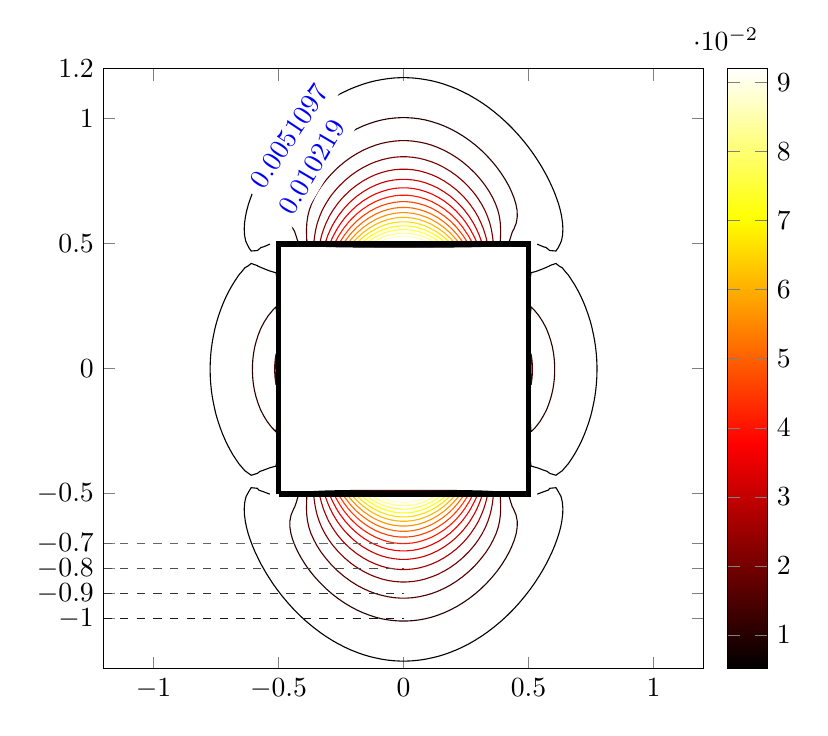
\begin{tikzpicture}

\begin{axis}[%
width=3in,
height=3in,
at={(0in,0in)},
scale only axis,
point meta min=0.0051,
point meta max=0.0920,
colormap/hot2,
xmin=-1.2000,
xmax=1.2000,
ymin=-1.2000,
ymax=1.2000,
ytick={-1.0000,-0.9000,-0.8000,-0.7000,-0.5000,0.0000,0.5000,1.0000,1.2000},
axis background/.style={fill=white},
colorbar
]
\addplot[contour prepared, contour prepared format=matlab, contour/labels=false] table[row sep=crcr] {%
%
0.0051	120.0000\\
-0.5348	0.4983\\
-0.5597	0.4878\\
-0.5701	0.4851\\
-0.5846	0.4729\\
-0.6095	0.4709\\
-0.6192	0.4851\\
-0.6311	0.5100\\
-0.6343	0.5250\\
-0.6360	0.5348\\
-0.6373	0.5597\\
-0.6359	0.5846\\
-0.6343	0.5945\\
-0.6323	0.6095\\
-0.6270	0.6343\\
-0.6201	0.6592\\
-0.6115	0.6841\\
-0.6095	0.6891\\
-0.6020	0.7090\\
-0.5912	0.7338\\
-0.5846	0.7474\\
-0.5793	0.7587\\
-0.5663	0.7836\\
-0.5597	0.7949\\
-0.5521	0.8085\\
-0.5366	0.8333\\
-0.5348	0.8359\\
-0.5201	0.8582\\
-0.5100	0.8723\\
-0.5022	0.8831\\
-0.4851	0.9048\\
-0.4826	0.9080\\
-0.4616	0.9328\\
-0.4602	0.9344\\
-0.4388	0.9577\\
-0.4353	0.9614\\
-0.4140	0.9826\\
-0.4104	0.9860\\
-0.3867	1.0075\\
-0.3856	1.0085\\
-0.3607	1.0292\\
-0.3567	1.0323\\
-0.3358	1.0483\\
-0.3229	1.0572\\
-0.3109	1.0655\\
-0.2861	1.0810\\
-0.2842	1.0821\\
-0.2612	1.0955\\
-0.2384	1.1070\\
-0.2363	1.1080\\
-0.2114	1.1197\\
-0.1866	1.1295\\
-0.1798	1.1318\\
-0.1617	1.1384\\
-0.1368	1.1459\\
-0.1119	1.1520\\
-0.0871	1.1567\\
-0.0869	1.1567\\
-0.0622	1.1605\\
-0.0373	1.1631\\
-0.0124	1.1643\\
0.0124	1.1643\\
0.0373	1.1631\\
0.0622	1.1605\\
0.0869	1.1567\\
0.0871	1.1567\\
0.1119	1.1520\\
0.1368	1.1459\\
0.1617	1.1384\\
0.1798	1.1318\\
0.1866	1.1295\\
0.2114	1.1197\\
0.2363	1.1080\\
0.2384	1.1070\\
0.2612	1.0955\\
0.2842	1.0821\\
0.2861	1.0810\\
0.3109	1.0655\\
0.3229	1.0572\\
0.3358	1.0483\\
0.3567	1.0323\\
0.3607	1.0292\\
0.3856	1.0085\\
0.3867	1.0075\\
0.4104	0.9860\\
0.4140	0.9826\\
0.4353	0.9614\\
0.4388	0.9577\\
0.4602	0.9344\\
0.4616	0.9328\\
0.4826	0.9080\\
0.4851	0.9048\\
0.5022	0.8831\\
0.5100	0.8723\\
0.5201	0.8582\\
0.5348	0.8359\\
0.5366	0.8333\\
0.5521	0.8085\\
0.5597	0.7949\\
0.5663	0.7836\\
0.5793	0.7587\\
0.5846	0.7474\\
0.5912	0.7338\\
0.6020	0.7090\\
0.6095	0.6891\\
0.6115	0.6841\\
0.6201	0.6592\\
0.6270	0.6343\\
0.6323	0.6095\\
0.6343	0.5945\\
0.6359	0.5846\\
0.6373	0.5597\\
0.6360	0.5348\\
0.6343	0.5250\\
0.6311	0.5100\\
0.6192	0.4851\\
0.6095	0.4709\\
0.5846	0.4729\\
0.5701	0.4851\\
0.5597	0.4878\\
0.5348	0.4983\\
0.0051	38.0000\\
-0.4602	-0.5070\\
-0.4353	-0.5000\\
-0.4104	-0.4960\\
-0.3856	-0.4933\\
-0.3607	-0.4914\\
-0.3358	-0.4901\\
-0.3109	-0.4891\\
-0.2861	-0.4885\\
-0.2612	-0.4879\\
-0.2363	-0.4875\\
-0.2114	-0.4872\\
-0.1866	-0.4870\\
-0.1617	-0.4868\\
-0.1368	-0.4867\\
-0.1119	-0.4866\\
-0.0871	-0.4865\\
-0.0622	-0.4864\\
-0.0373	-0.4864\\
-0.0124	-0.4864\\
0.0124	-0.4864\\
0.0373	-0.4864\\
0.0622	-0.4864\\
0.0871	-0.4865\\
0.1119	-0.4866\\
0.1368	-0.4867\\
0.1617	-0.4868\\
0.1866	-0.4870\\
0.2114	-0.4872\\
0.2363	-0.4875\\
0.2612	-0.4879\\
0.2861	-0.4885\\
0.3109	-0.4891\\
0.3358	-0.4901\\
0.3607	-0.4914\\
0.3856	-0.4933\\
0.4104	-0.4960\\
0.4353	-0.5000\\
0.4602	-0.5070\\
0.0051	38.0000\\
0.4602	0.5065\\
0.4353	0.4997\\
0.4104	0.4958\\
0.3856	0.4932\\
0.3607	0.4914\\
0.3358	0.4901\\
0.3109	0.4892\\
0.2861	0.4885\\
0.2612	0.4880\\
0.2363	0.4876\\
0.2114	0.4873\\
0.1866	0.4870\\
0.1617	0.4869\\
0.1368	0.4867\\
0.1119	0.4866\\
0.0871	0.4865\\
0.0622	0.4865\\
0.0373	0.4864\\
0.0124	0.4864\\
-0.0124	0.4864\\
-0.0373	0.4864\\
-0.0622	0.4865\\
-0.0871	0.4865\\
-0.1119	0.4866\\
-0.1368	0.4867\\
-0.1617	0.4869\\
-0.1866	0.4870\\
-0.2114	0.4873\\
-0.2363	0.4876\\
-0.2612	0.4880\\
-0.2861	0.4885\\
-0.3109	0.4892\\
-0.3358	0.4901\\
-0.3607	0.4914\\
-0.3856	0.4932\\
-0.4104	0.4958\\
-0.4353	0.4997\\
-0.4602	0.5065\\
0.0051	120.0000\\
0.5348	-0.5016\\
0.5597	-0.4922\\
0.5796	-0.4851\\
0.5846	-0.4783\\
0.6095	-0.4758\\
0.6155	-0.4851\\
0.6295	-0.5100\\
0.6343	-0.5294\\
0.6353	-0.5348\\
0.6373	-0.5597\\
0.6364	-0.5846\\
0.6343	-0.5995\\
0.6331	-0.6095\\
0.6282	-0.6343\\
0.6216	-0.6592\\
0.6133	-0.6841\\
0.6095	-0.6940\\
0.6040	-0.7090\\
0.5935	-0.7338\\
0.5846	-0.7524\\
0.5817	-0.7587\\
0.5690	-0.7836\\
0.5597	-0.7999\\
0.5550	-0.8085\\
0.5398	-0.8333\\
0.5348	-0.8409\\
0.5236	-0.8582\\
0.5100	-0.8772\\
0.5058	-0.8831\\
0.4866	-0.9080\\
0.4851	-0.9098\\
0.4660	-0.9328\\
0.4602	-0.9394\\
0.4436	-0.9577\\
0.4353	-0.9664\\
0.4192	-0.9826\\
0.4104	-0.9911\\
0.3925	-1.0075\\
0.3856	-1.0136\\
0.3629	-1.0323\\
0.3607	-1.0342\\
0.3358	-1.0531\\
0.3300	-1.0572\\
0.3109	-1.0705\\
0.2924	-1.0821\\
0.2861	-1.0861\\
0.2612	-1.1004\\
0.2482	-1.1070\\
0.2363	-1.1132\\
0.2114	-1.1246\\
0.1930	-1.1318\\
0.1866	-1.1345\\
0.1617	-1.1434\\
0.1368	-1.1508\\
0.1120	-1.1567\\
0.1119	-1.1567\\
0.0871	-1.1619\\
0.0622	-1.1656\\
0.0373	-1.1681\\
0.0124	-1.1694\\
-0.0124	-1.1694\\
-0.0373	-1.1681\\
-0.0622	-1.1656\\
-0.0871	-1.1619\\
-0.1119	-1.1567\\
-0.1120	-1.1567\\
-0.1368	-1.1508\\
-0.1617	-1.1434\\
-0.1866	-1.1345\\
-0.1930	-1.1318\\
-0.2114	-1.1246\\
-0.2363	-1.1132\\
-0.2482	-1.1070\\
-0.2612	-1.1004\\
-0.2861	-1.0861\\
-0.2924	-1.0821\\
-0.3109	-1.0705\\
-0.3300	-1.0572\\
-0.3358	-1.0531\\
-0.3607	-1.0342\\
-0.3629	-1.0323\\
-0.3856	-1.0136\\
-0.3925	-1.0075\\
-0.4104	-0.9911\\
-0.4192	-0.9826\\
-0.4353	-0.9664\\
-0.4436	-0.9577\\
-0.4602	-0.9394\\
-0.4660	-0.9328\\
-0.4851	-0.9098\\
-0.4866	-0.9080\\
-0.5058	-0.8831\\
-0.5100	-0.8772\\
-0.5236	-0.8582\\
-0.5348	-0.8409\\
-0.5398	-0.8333\\
-0.5550	-0.8085\\
-0.5597	-0.7999\\
-0.5690	-0.7836\\
-0.5817	-0.7587\\
-0.5846	-0.7524\\
-0.5935	-0.7338\\
-0.6040	-0.7090\\
-0.6095	-0.6940\\
-0.6133	-0.6841\\
-0.6216	-0.6592\\
-0.6282	-0.6343\\
-0.6331	-0.6095\\
-0.6343	-0.5995\\
-0.6364	-0.5846\\
-0.6373	-0.5597\\
-0.6353	-0.5348\\
-0.6343	-0.5294\\
-0.6295	-0.5100\\
-0.6155	-0.4851\\
-0.6095	-0.4758\\
-0.5846	-0.4783\\
-0.5796	-0.4851\\
-0.5597	-0.4922\\
-0.5348	-0.5016\\
0.0051	91.0000\\
-0.7587	-0.1454\\
-0.7606	-0.1368\\
-0.7651	-0.1119\\
-0.7686	-0.0871\\
-0.7712	-0.0622\\
-0.7729	-0.0373\\
-0.7736	-0.0124\\
-0.7736	0.0124\\
-0.7726	0.0373\\
-0.7708	0.0622\\
-0.7680	0.0871\\
-0.7643	0.1119\\
-0.7596	0.1368\\
-0.7587	0.1406\\
-0.7542	0.1617\\
-0.7478	0.1866\\
-0.7402	0.2114\\
-0.7338	0.2297\\
-0.7315	0.2363\\
-0.7219	0.2612\\
-0.7108	0.2861\\
-0.7090	0.2899\\
-0.6984	0.3109\\
-0.6845	0.3358\\
-0.6841	0.3365\\
-0.6684	0.3607\\
-0.6592	0.3747\\
-0.6495	0.3856\\
-0.6343	0.4043\\
-0.6230	0.4104\\
-0.6095	0.4212\\
-0.5846	0.4125\\
-0.5827	0.4104\\
-0.5597	0.4007\\
-0.5348	0.3910\\
-0.5161	0.3856\\
-0.5100	0.3843\\
-0.5065	0.3607\\
-0.5036	0.3358\\
-0.5014	0.3109\\
-0.4996	0.2861\\
-0.4982	0.2612\\
-0.4970	0.2363\\
-0.4961	0.2114\\
-0.4954	0.1866\\
-0.4948	0.1617\\
-0.4943	0.1368\\
-0.4939	0.1119\\
-0.4936	0.0871\\
-0.4934	0.0622\\
-0.4932	0.0373\\
-0.4932	0.0124\\
-0.4932	-0.0124\\
-0.4932	-0.0373\\
-0.4933	-0.0622\\
-0.4935	-0.0871\\
-0.4938	-0.1119\\
-0.4942	-0.1368\\
-0.4946	-0.1617\\
-0.4952	-0.1866\\
-0.4959	-0.2114\\
-0.4968	-0.2363\\
-0.4979	-0.2612\\
-0.4993	-0.2861\\
-0.5010	-0.3109\\
-0.5032	-0.3358\\
-0.5059	-0.3607\\
-0.5094	-0.3856\\
-0.5100	-0.3894\\
-0.5348	-0.3961\\
-0.5597	-0.4055\\
-0.5743	-0.4104\\
-0.5846	-0.4185\\
-0.6095	-0.4260\\
-0.6310	-0.4104\\
-0.6343	-0.4086\\
-0.6538	-0.3856\\
-0.6592	-0.3795\\
-0.6718	-0.3607\\
-0.6841	-0.3417\\
-0.6874	-0.3358\\
-0.7010	-0.3109\\
-0.7090	-0.2949\\
-0.7131	-0.2861\\
-0.7239	-0.2612\\
-0.7333	-0.2363\\
-0.7338	-0.2347\\
-0.7418	-0.2114\\
-0.7492	-0.1866\\
-0.7553	-0.1617\\
-0.7587	-0.1454\\
0.0051	91.0000\\
0.5100	-0.3894\\
0.5094	-0.3856\\
0.5059	-0.3607\\
0.5032	-0.3358\\
0.5010	-0.3109\\
0.4993	-0.2861\\
0.4979	-0.2612\\
0.4968	-0.2363\\
0.4959	-0.2114\\
0.4952	-0.1866\\
0.4946	-0.1617\\
0.4942	-0.1368\\
0.4938	-0.1119\\
0.4935	-0.0871\\
0.4933	-0.0622\\
0.4932	-0.0373\\
0.4932	-0.0124\\
0.4932	0.0124\\
0.4932	0.0373\\
0.4934	0.0622\\
0.4936	0.0871\\
0.4939	0.1119\\
0.4943	0.1368\\
0.4948	0.1617\\
0.4954	0.1866\\
0.4961	0.2114\\
0.4970	0.2363\\
0.4982	0.2612\\
0.4996	0.2861\\
0.5014	0.3109\\
0.5036	0.3358\\
0.5065	0.3607\\
0.5100	0.3843\\
0.5161	0.3856\\
0.5348	0.3910\\
0.5597	0.4007\\
0.5827	0.4104\\
0.5846	0.4125\\
0.6095	0.4212\\
0.6230	0.4104\\
0.6343	0.4043\\
0.6495	0.3856\\
0.6592	0.3747\\
0.6684	0.3607\\
0.6841	0.3365\\
0.6845	0.3358\\
0.6984	0.3109\\
0.7090	0.2899\\
0.7108	0.2861\\
0.7219	0.2612\\
0.7315	0.2363\\
0.7338	0.2297\\
0.7402	0.2114\\
0.7478	0.1866\\
0.7542	0.1617\\
0.7587	0.1406\\
0.7596	0.1368\\
0.7643	0.1119\\
0.7680	0.0871\\
0.7708	0.0622\\
0.7726	0.0373\\
0.7736	0.0124\\
0.7736	-0.0124\\
0.7729	-0.0373\\
0.7712	-0.0622\\
0.7686	-0.0871\\
0.7651	-0.1119\\
0.7606	-0.1368\\
0.7587	-0.1454\\
0.7553	-0.1617\\
0.7492	-0.1866\\
0.7418	-0.2114\\
0.7338	-0.2347\\
0.7333	-0.2363\\
0.7239	-0.2612\\
0.7131	-0.2861\\
0.7090	-0.2949\\
0.7010	-0.3109\\
0.6874	-0.3358\\
0.6841	-0.3417\\
0.6718	-0.3607\\
0.6592	-0.3795\\
0.6538	-0.3856\\
0.6343	-0.4086\\
0.6310	-0.4104\\
0.6095	-0.4260\\
0.5846	-0.4185\\
0.5743	-0.4104\\
0.5597	-0.4055\\
0.5348	-0.3961\\
0.5100	-0.3894\\
0.0102	49.0000\\
-0.5846	-0.1299\\
-0.5903	-0.1119\\
-0.5964	-0.0871\\
-0.6006	-0.0622\\
-0.6033	-0.0373\\
-0.6045	-0.0124\\
-0.6044	0.0124\\
-0.6029	0.0373\\
-0.5999	0.0622\\
-0.5953	0.0871\\
-0.5889	0.1119\\
-0.5846	0.1248\\
-0.5808	0.1368\\
-0.5708	0.1617\\
-0.5597	0.1827\\
-0.5577	0.1866\\
-0.5418	0.2114\\
-0.5348	0.2201\\
-0.5213	0.2363\\
-0.5100	0.2472\\
-0.5090	0.2363\\
-0.5071	0.2114\\
-0.5056	0.1866\\
-0.5044	0.1617\\
-0.5035	0.1368\\
-0.5027	0.1119\\
-0.5021	0.0871\\
-0.5017	0.0622\\
-0.5014	0.0373\\
-0.5013	0.0124\\
-0.5012	-0.0124\\
-0.5014	-0.0373\\
-0.5016	-0.0622\\
-0.5020	-0.0871\\
-0.5026	-0.1119\\
-0.5033	-0.1368\\
-0.5042	-0.1617\\
-0.5054	-0.1866\\
-0.5068	-0.2114\\
-0.5086	-0.2363\\
-0.5100	-0.2522\\
-0.5259	-0.2363\\
-0.5348	-0.2251\\
-0.5454	-0.2114\\
-0.5597	-0.1877\\
-0.5604	-0.1866\\
-0.5730	-0.1617\\
-0.5825	-0.1368\\
-0.5846	-0.1299\\
0.0102	115.0000\\
-0.4353	-0.7044\\
-0.4434	-0.6841\\
-0.4505	-0.6592\\
-0.4545	-0.6343\\
-0.4547	-0.6095\\
-0.4499	-0.5846\\
-0.4393	-0.5597\\
-0.4353	-0.5527\\
-0.4291	-0.5348\\
-0.4219	-0.5100\\
-0.4104	-0.5068\\
-0.3856	-0.5014\\
-0.3607	-0.4977\\
-0.3358	-0.4951\\
-0.3109	-0.4932\\
-0.2861	-0.4918\\
-0.2612	-0.4908\\
-0.2363	-0.4900\\
-0.2114	-0.4894\\
-0.1866	-0.4889\\
-0.1617	-0.4886\\
-0.1368	-0.4883\\
-0.1119	-0.4881\\
-0.0871	-0.4879\\
-0.0622	-0.4878\\
-0.0373	-0.4877\\
-0.0124	-0.4877\\
0.0124	-0.4877\\
0.0373	-0.4877\\
0.0622	-0.4878\\
0.0871	-0.4879\\
0.1119	-0.4881\\
0.1368	-0.4883\\
0.1617	-0.4886\\
0.1866	-0.4889\\
0.2114	-0.4894\\
0.2363	-0.4900\\
0.2612	-0.4908\\
0.2861	-0.4918\\
0.3109	-0.4932\\
0.3358	-0.4951\\
0.3607	-0.4977\\
0.3856	-0.5014\\
0.4104	-0.5068\\
0.4219	-0.5100\\
0.4291	-0.5348\\
0.4353	-0.5527\\
0.4393	-0.5597\\
0.4499	-0.5846\\
0.4547	-0.6095\\
0.4545	-0.6343\\
0.4505	-0.6592\\
0.4434	-0.6841\\
0.4353	-0.7044\\
0.4336	-0.7090\\
0.4223	-0.7338\\
0.4104	-0.7549\\
0.4083	-0.7587\\
0.3928	-0.7836\\
0.3856	-0.7937\\
0.3749	-0.8085\\
0.3607	-0.8262\\
0.3547	-0.8333\\
0.3358	-0.8541\\
0.3319	-0.8582\\
0.3109	-0.8788\\
0.3062	-0.8831\\
0.2861	-0.9006\\
0.2767	-0.9080\\
0.2612	-0.9199\\
0.2422	-0.9328\\
0.2363	-0.9368\\
0.2114	-0.9519\\
0.2003	-0.9577\\
0.1866	-0.9650\\
0.1617	-0.9763\\
0.1450	-0.9826\\
0.1368	-0.9858\\
0.1119	-0.9939\\
0.0871	-1.0001\\
0.0622	-1.0046\\
0.0383	-1.0075\\
0.0373	-1.0076\\
0.0124	-1.0092\\
-0.0124	-1.0092\\
-0.0373	-1.0076\\
-0.0383	-1.0075\\
-0.0622	-1.0046\\
-0.0871	-1.0001\\
-0.1119	-0.9939\\
-0.1368	-0.9858\\
-0.1450	-0.9826\\
-0.1617	-0.9763\\
-0.1866	-0.9650\\
-0.2003	-0.9577\\
-0.2114	-0.9519\\
-0.2363	-0.9368\\
-0.2422	-0.9328\\
-0.2612	-0.9199\\
-0.2767	-0.9080\\
-0.2861	-0.9006\\
-0.3062	-0.8831\\
-0.3109	-0.8788\\
-0.3319	-0.8582\\
-0.3358	-0.8541\\
-0.3547	-0.8333\\
-0.3607	-0.8262\\
-0.3749	-0.8085\\
-0.3856	-0.7937\\
-0.3928	-0.7836\\
-0.4083	-0.7587\\
-0.4104	-0.7549\\
-0.4223	-0.7338\\
-0.4336	-0.7090\\
-0.4353	-0.7044\\
0.0102	113.0000\\
-0.4353	0.5481\\
-0.4418	0.5597\\
-0.4513	0.5846\\
-0.4550	0.6095\\
-0.4540	0.6343\\
-0.4493	0.6592\\
-0.4416	0.6841\\
-0.4353	0.6993\\
-0.4316	0.7090\\
-0.4197	0.7338\\
-0.4104	0.7499\\
-0.4055	0.7587\\
-0.3893	0.7836\\
-0.3856	0.7887\\
-0.3711	0.8085\\
-0.3607	0.8212\\
-0.3504	0.8333\\
-0.3358	0.8492\\
-0.3271	0.8582\\
-0.3109	0.8739\\
-0.3006	0.8831\\
-0.2861	0.8957\\
-0.2702	0.9080\\
-0.2612	0.9149\\
-0.2363	0.9318\\
-0.2345	0.9328\\
-0.2114	0.9470\\
-0.1907	0.9577\\
-0.1866	0.9599\\
-0.1617	0.9714\\
-0.1368	0.9808\\
-0.1309	0.9826\\
-0.1119	0.9888\\
-0.0871	0.9952\\
-0.0622	0.9998\\
-0.0373	1.0028\\
-0.0124	1.0043\\
0.0124	1.0043\\
0.0373	1.0028\\
0.0622	0.9998\\
0.0871	0.9952\\
0.1119	0.9888\\
0.1309	0.9826\\
0.1368	0.9808\\
0.1617	0.9714\\
0.1866	0.9599\\
0.1907	0.9577\\
0.2114	0.9470\\
0.2345	0.9328\\
0.2363	0.9318\\
0.2612	0.9149\\
0.2702	0.9080\\
0.2861	0.8957\\
0.3006	0.8831\\
0.3109	0.8739\\
0.3271	0.8582\\
0.3358	0.8492\\
0.3504	0.8333\\
0.3607	0.8212\\
0.3711	0.8085\\
0.3856	0.7887\\
0.3893	0.7836\\
0.4055	0.7587\\
0.4104	0.7499\\
0.4197	0.7338\\
0.4316	0.7090\\
0.4353	0.6993\\
0.4416	0.6841\\
0.4493	0.6592\\
0.4540	0.6343\\
0.4550	0.6095\\
0.4513	0.5846\\
0.4418	0.5597\\
0.4353	0.5481\\
0.4309	0.5348\\
0.4232	0.5100\\
0.4104	0.5066\\
0.3856	0.5014\\
0.3607	0.4978\\
0.3358	0.4952\\
0.3109	0.4933\\
0.2861	0.4919\\
0.2612	0.4909\\
0.2363	0.4901\\
0.2114	0.4895\\
0.1866	0.4890\\
0.1617	0.4886\\
0.1368	0.4884\\
0.1119	0.4881\\
0.0871	0.4880\\
0.0622	0.4879\\
0.0373	0.4878\\
0.0124	0.4878\\
-0.0124	0.4878\\
-0.0373	0.4878\\
-0.0622	0.4879\\
-0.0871	0.4880\\
-0.1119	0.4881\\
-0.1368	0.4884\\
-0.1617	0.4886\\
-0.1866	0.4890\\
-0.2114	0.4895\\
-0.2363	0.4901\\
-0.2612	0.4909\\
-0.2861	0.4919\\
-0.3109	0.4933\\
-0.3358	0.4952\\
-0.3607	0.4978\\
-0.3856	0.5014\\
-0.4104	0.5066\\
-0.4232	0.5100\\
-0.4309	0.5348\\
-0.4353	0.5481\\
0.0102	49.0000\\
0.5100	-0.2522\\
0.5086	-0.2363\\
0.5068	-0.2114\\
0.5054	-0.1866\\
0.5042	-0.1617\\
0.5033	-0.1368\\
0.5026	-0.1119\\
0.5020	-0.0871\\
0.5016	-0.0622\\
0.5014	-0.0373\\
0.5012	-0.0124\\
0.5013	0.0124\\
0.5014	0.0373\\
0.5017	0.0622\\
0.5021	0.0871\\
0.5027	0.1119\\
0.5035	0.1368\\
0.5044	0.1617\\
0.5056	0.1866\\
0.5071	0.2114\\
0.5090	0.2363\\
0.5100	0.2472\\
0.5213	0.2363\\
0.5348	0.2201\\
0.5418	0.2114\\
0.5577	0.1866\\
0.5597	0.1827\\
0.5708	0.1617\\
0.5808	0.1368\\
0.5846	0.1248\\
0.5889	0.1119\\
0.5953	0.0871\\
0.5999	0.0622\\
0.6029	0.0373\\
0.6044	0.0124\\
0.6045	-0.0124\\
0.6033	-0.0373\\
0.6006	-0.0622\\
0.5964	-0.0871\\
0.5903	-0.1119\\
0.5846	-0.1299\\
0.5825	-0.1368\\
0.5730	-0.1617\\
0.5604	-0.1866\\
0.5597	-0.1877\\
0.5454	-0.2114\\
0.5348	-0.2251\\
0.5259	-0.2363\\
0.5100	-0.2522\\
0.0153	13.0000\\
-0.5100	-0.0649\\
-0.5105	-0.0622\\
-0.5139	-0.0373\\
-0.5155	-0.0124\\
-0.5154	0.0124\\
-0.5134	0.0373\\
-0.5100	0.0600\\
-0.5096	0.0373\\
-0.5094	0.0124\\
-0.5093	-0.0124\\
-0.5095	-0.0373\\
-0.5099	-0.0622\\
-0.5100	-0.0649\\
0.0153	99.0000\\
-0.3856	-0.5974\\
-0.3873	-0.5846\\
-0.3883	-0.5597\\
-0.3879	-0.5348\\
-0.3869	-0.5100\\
-0.3856	-0.5096\\
-0.3607	-0.5041\\
-0.3358	-0.5001\\
-0.3109	-0.4973\\
-0.2861	-0.4952\\
-0.2612	-0.4936\\
-0.2363	-0.4925\\
-0.2114	-0.4916\\
-0.1866	-0.4909\\
-0.1617	-0.4903\\
-0.1368	-0.4899\\
-0.1119	-0.4896\\
-0.0871	-0.4893\\
-0.0622	-0.4892\\
-0.0373	-0.4891\\
-0.0124	-0.4890\\
0.0124	-0.4890\\
0.0373	-0.4891\\
0.0622	-0.4892\\
0.0871	-0.4893\\
0.1119	-0.4896\\
0.1368	-0.4899\\
0.1617	-0.4903\\
0.1866	-0.4909\\
0.2114	-0.4916\\
0.2363	-0.4925\\
0.2612	-0.4936\\
0.2861	-0.4952\\
0.3109	-0.4973\\
0.3358	-0.5001\\
0.3607	-0.5041\\
0.3856	-0.5096\\
0.3869	-0.5100\\
0.3879	-0.5348\\
0.3883	-0.5597\\
0.3873	-0.5846\\
0.3856	-0.5974\\
0.3841	-0.6095\\
0.3785	-0.6343\\
0.3702	-0.6592\\
0.3607	-0.6801\\
0.3589	-0.6841\\
0.3457	-0.7090\\
0.3358	-0.7244\\
0.3296	-0.7338\\
0.3109	-0.7584\\
0.3107	-0.7587\\
0.2891	-0.7836\\
0.2861	-0.7869\\
0.2640	-0.8085\\
0.2612	-0.8110\\
0.2363	-0.8319\\
0.2344	-0.8333\\
0.2114	-0.8501\\
0.1985	-0.8582\\
0.1866	-0.8657\\
0.1617	-0.8789\\
0.1523	-0.8831\\
0.1368	-0.8902\\
0.1119	-0.8994\\
0.0871	-0.9065\\
0.0799	-0.9080\\
0.0622	-0.9120\\
0.0373	-0.9157\\
0.0124	-0.9175\\
-0.0124	-0.9175\\
-0.0373	-0.9157\\
-0.0622	-0.9120\\
-0.0799	-0.9080\\
-0.0871	-0.9065\\
-0.1119	-0.8994\\
-0.1368	-0.8902\\
-0.1523	-0.8831\\
-0.1617	-0.8789\\
-0.1866	-0.8657\\
-0.1985	-0.8582\\
-0.2114	-0.8501\\
-0.2344	-0.8333\\
-0.2363	-0.8319\\
-0.2612	-0.8110\\
-0.2640	-0.8085\\
-0.2861	-0.7869\\
-0.2891	-0.7836\\
-0.3107	-0.7587\\
-0.3109	-0.7584\\
-0.3296	-0.7338\\
-0.3358	-0.7244\\
-0.3457	-0.7090\\
-0.3589	-0.6841\\
-0.3607	-0.6801\\
-0.3702	-0.6592\\
-0.3785	-0.6343\\
-0.3841	-0.6095\\
-0.3856	-0.5974\\
0.0153	99.0000\\
-0.3856	0.5096\\
-0.3871	0.5100\\
-0.3880	0.5348\\
-0.3882	0.5597\\
-0.3868	0.5846\\
-0.3856	0.5927\\
-0.3832	0.6095\\
-0.3771	0.6343\\
-0.3681	0.6592\\
-0.3607	0.6751\\
-0.3565	0.6841\\
-0.3426	0.7090\\
-0.3358	0.7194\\
-0.3261	0.7338\\
-0.3109	0.7536\\
-0.3067	0.7587\\
-0.2861	0.7819\\
-0.2844	0.7836\\
-0.2612	0.8061\\
-0.2584	0.8085\\
-0.2363	0.8271\\
-0.2278	0.8333\\
-0.2114	0.8452\\
-0.1904	0.8582\\
-0.1866	0.8606\\
-0.1617	0.8741\\
-0.1411	0.8831\\
-0.1368	0.8851\\
-0.1119	0.8945\\
-0.0871	0.9017\\
-0.0622	0.9069\\
-0.0543	0.9080\\
-0.0373	0.9105\\
-0.0124	0.9124\\
0.0124	0.9124\\
0.0373	0.9105\\
0.0543	0.9080\\
0.0622	0.9069\\
0.0871	0.9017\\
0.1119	0.8945\\
0.1368	0.8851\\
0.1411	0.8831\\
0.1617	0.8741\\
0.1866	0.8606\\
0.1904	0.8582\\
0.2114	0.8452\\
0.2278	0.8333\\
0.2363	0.8271\\
0.2584	0.8085\\
0.2612	0.8061\\
0.2844	0.7836\\
0.2861	0.7819\\
0.3067	0.7587\\
0.3109	0.7536\\
0.3261	0.7338\\
0.3358	0.7194\\
0.3426	0.7090\\
0.3565	0.6841\\
0.3607	0.6751\\
0.3681	0.6592\\
0.3771	0.6343\\
0.3832	0.6095\\
0.3856	0.5927\\
0.3868	0.5846\\
0.3882	0.5597\\
0.3880	0.5348\\
0.3871	0.5100\\
0.3856	0.5096\\
0.3607	0.5042\\
0.3358	0.5003\\
0.3109	0.4975\\
0.2861	0.4954\\
0.2612	0.4938\\
0.2363	0.4926\\
0.2114	0.4917\\
0.1866	0.4910\\
0.1617	0.4904\\
0.1368	0.4900\\
0.1119	0.4897\\
0.0871	0.4894\\
0.0622	0.4893\\
0.0373	0.4891\\
0.0124	0.4891\\
-0.0124	0.4891\\
-0.0373	0.4891\\
-0.0622	0.4893\\
-0.0871	0.4894\\
-0.1119	0.4897\\
-0.1368	0.4900\\
-0.1617	0.4904\\
-0.1866	0.4910\\
-0.2114	0.4917\\
-0.2363	0.4926\\
-0.2612	0.4938\\
-0.2861	0.4954\\
-0.3109	0.4975\\
-0.3358	0.5003\\
-0.3607	0.5042\\
-0.3856	0.5096\\
0.0153	13.0000\\
0.5100	-0.0649\\
0.5099	-0.0622\\
0.5095	-0.0373\\
0.5093	-0.0124\\
0.5094	0.0124\\
0.5096	0.0373\\
0.5100	0.0600\\
0.5134	0.0373\\
0.5154	0.0124\\
0.5155	-0.0124\\
0.5139	-0.0373\\
0.5105	-0.0622\\
0.5100	-0.0649\\
0.0204	85.0000\\
-0.3358	-0.6138\\
-0.3376	-0.6095\\
-0.3458	-0.5846\\
-0.3517	-0.5597\\
-0.3559	-0.5348\\
-0.3590	-0.5100\\
-0.3358	-0.5052\\
-0.3109	-0.5014\\
-0.2861	-0.4986\\
-0.2612	-0.4965\\
-0.2363	-0.4949\\
-0.2114	-0.4937\\
-0.1866	-0.4928\\
-0.1617	-0.4921\\
-0.1368	-0.4915\\
-0.1119	-0.4911\\
-0.0871	-0.4908\\
-0.0622	-0.4905\\
-0.0373	-0.4904\\
-0.0124	-0.4903\\
0.0124	-0.4903\\
0.0373	-0.4904\\
0.0622	-0.4905\\
0.0871	-0.4908\\
0.1119	-0.4911\\
0.1368	-0.4915\\
0.1617	-0.4921\\
0.1866	-0.4928\\
0.2114	-0.4937\\
0.2363	-0.4949\\
0.2612	-0.4965\\
0.2861	-0.4986\\
0.3109	-0.5014\\
0.3358	-0.5052\\
0.3590	-0.5100\\
0.3559	-0.5348\\
0.3517	-0.5597\\
0.3458	-0.5846\\
0.3376	-0.6095\\
0.3358	-0.6138\\
0.3275	-0.6343\\
0.3145	-0.6592\\
0.3109	-0.6653\\
0.2992	-0.6841\\
0.2861	-0.7022\\
0.2808	-0.7090\\
0.2612	-0.7317\\
0.2591	-0.7338\\
0.2363	-0.7563\\
0.2335	-0.7587\\
0.2114	-0.7773\\
0.2027	-0.7836\\
0.1866	-0.7951\\
0.1640	-0.8085\\
0.1617	-0.8099\\
0.1368	-0.8226\\
0.1119	-0.8326\\
0.1096	-0.8333\\
0.0871	-0.8409\\
0.0622	-0.8470\\
0.0373	-0.8509\\
0.0124	-0.8528\\
-0.0124	-0.8528\\
-0.0373	-0.8509\\
-0.0622	-0.8470\\
-0.0871	-0.8409\\
-0.1096	-0.8333\\
-0.1119	-0.8326\\
-0.1368	-0.8226\\
-0.1617	-0.8099\\
-0.1640	-0.8085\\
-0.1866	-0.7951\\
-0.2027	-0.7836\\
-0.2114	-0.7773\\
-0.2335	-0.7587\\
-0.2363	-0.7563\\
-0.2591	-0.7338\\
-0.2612	-0.7317\\
-0.2808	-0.7090\\
-0.2861	-0.7022\\
-0.2992	-0.6841\\
-0.3109	-0.6653\\
-0.3145	-0.6592\\
-0.3275	-0.6343\\
-0.3358	-0.6138\\
0.0204	85.0000\\
-0.3358	0.5054\\
-0.3584	0.5100\\
-0.3552	0.5348\\
-0.3507	0.5597\\
-0.3444	0.5846\\
-0.3358	0.6089\\
-0.3356	0.6095\\
-0.3251	0.6343\\
-0.3116	0.6592\\
-0.3109	0.6602\\
-0.2958	0.6841\\
-0.2861	0.6973\\
-0.2768	0.7090\\
-0.2612	0.7268\\
-0.2544	0.7338\\
-0.2363	0.7515\\
-0.2279	0.7587\\
-0.2114	0.7724\\
-0.1957	0.7836\\
-0.1866	0.7901\\
-0.1617	0.8050\\
-0.1547	0.8085\\
-0.1368	0.8177\\
-0.1119	0.8278\\
-0.0944	0.8333\\
-0.0871	0.8358\\
-0.0622	0.8419\\
-0.0373	0.8459\\
-0.0124	0.8479\\
0.0124	0.8479\\
0.0373	0.8459\\
0.0622	0.8419\\
0.0871	0.8358\\
0.0944	0.8333\\
0.1119	0.8278\\
0.1368	0.8177\\
0.1547	0.8085\\
0.1617	0.8050\\
0.1866	0.7901\\
0.1957	0.7836\\
0.2114	0.7724\\
0.2279	0.7587\\
0.2363	0.7515\\
0.2544	0.7338\\
0.2612	0.7268\\
0.2768	0.7090\\
0.2861	0.6973\\
0.2958	0.6841\\
0.3109	0.6602\\
0.3116	0.6592\\
0.3251	0.6343\\
0.3356	0.6095\\
0.3358	0.6089\\
0.3444	0.5846\\
0.3507	0.5597\\
0.3552	0.5348\\
0.3584	0.5100\\
0.3358	0.5054\\
0.3109	0.5016\\
0.2861	0.4988\\
0.2612	0.4967\\
0.2363	0.4951\\
0.2114	0.4939\\
0.1866	0.4929\\
0.1617	0.4922\\
0.1368	0.4916\\
0.1119	0.4912\\
0.0871	0.4909\\
0.0622	0.4907\\
0.0373	0.4905\\
0.0124	0.4904\\
-0.0124	0.4904\\
-0.0373	0.4905\\
-0.0622	0.4907\\
-0.0871	0.4909\\
-0.1119	0.4912\\
-0.1368	0.4916\\
-0.1617	0.4922\\
-0.1866	0.4929\\
-0.2114	0.4939\\
-0.2363	0.4951\\
-0.2612	0.4967\\
-0.2861	0.4988\\
-0.3109	0.5016\\
-0.3358	0.5054\\
0.0255	77.0000\\
-0.3109	-0.5852\\
-0.3112	-0.5846\\
-0.3210	-0.5597\\
-0.3287	-0.5348\\
-0.3348	-0.5100\\
-0.3109	-0.5054\\
-0.2861	-0.5020\\
-0.2612	-0.4994\\
-0.2363	-0.4974\\
-0.2114	-0.4959\\
-0.1866	-0.4947\\
-0.1617	-0.4938\\
-0.1368	-0.4931\\
-0.1119	-0.4926\\
-0.0871	-0.4922\\
-0.0622	-0.4919\\
-0.0373	-0.4917\\
-0.0124	-0.4916\\
0.0124	-0.4916\\
0.0373	-0.4917\\
0.0622	-0.4919\\
0.0871	-0.4922\\
0.1119	-0.4926\\
0.1368	-0.4931\\
0.1617	-0.4938\\
0.1866	-0.4947\\
0.2114	-0.4959\\
0.2363	-0.4974\\
0.2612	-0.4994\\
0.2861	-0.5020\\
0.3109	-0.5054\\
0.3348	-0.5100\\
0.3287	-0.5348\\
0.3210	-0.5597\\
0.3112	-0.5846\\
0.3109	-0.5852\\
0.2997	-0.6095\\
0.2861	-0.6331\\
0.2853	-0.6343\\
0.2684	-0.6592\\
0.2612	-0.6687\\
0.2482	-0.6841\\
0.2363	-0.6971\\
0.2240	-0.7090\\
0.2114	-0.7206\\
0.1947	-0.7338\\
0.1866	-0.7401\\
0.1617	-0.7565\\
0.1576	-0.7587\\
0.1368	-0.7704\\
0.1119	-0.7813\\
0.1052	-0.7836\\
0.0871	-0.7902\\
0.0622	-0.7967\\
0.0373	-0.8009\\
0.0124	-0.8030\\
-0.0124	-0.8030\\
-0.0373	-0.8009\\
-0.0622	-0.7967\\
-0.0871	-0.7902\\
-0.1052	-0.7836\\
-0.1119	-0.7813\\
-0.1368	-0.7704\\
-0.1576	-0.7587\\
-0.1617	-0.7565\\
-0.1866	-0.7401\\
-0.1947	-0.7338\\
-0.2114	-0.7206\\
-0.2240	-0.7090\\
-0.2363	-0.6971\\
-0.2482	-0.6841\\
-0.2612	-0.6687\\
-0.2684	-0.6592\\
-0.2853	-0.6343\\
-0.2861	-0.6331\\
-0.2997	-0.6095\\
-0.3109	-0.5852\\
0.0255	77.0000\\
-0.3109	0.5057\\
-0.3337	0.5100\\
-0.3273	0.5348\\
-0.3193	0.5597\\
-0.3109	0.5803\\
-0.3091	0.5846\\
-0.2971	0.6095\\
-0.2861	0.6282\\
-0.2822	0.6343\\
-0.2646	0.6592\\
-0.2612	0.6636\\
-0.2437	0.6841\\
-0.2363	0.6921\\
-0.2186	0.7090\\
-0.2114	0.7155\\
-0.1881	0.7338\\
-0.1866	0.7350\\
-0.1617	0.7517\\
-0.1487	0.7587\\
-0.1368	0.7653\\
-0.1119	0.7765\\
-0.0910	0.7836\\
-0.0871	0.7850\\
-0.0622	0.7917\\
-0.0373	0.7960\\
-0.0124	0.7981\\
0.0124	0.7981\\
0.0373	0.7960\\
0.0622	0.7917\\
0.0871	0.7850\\
0.0910	0.7836\\
0.1119	0.7765\\
0.1368	0.7653\\
0.1487	0.7587\\
0.1617	0.7517\\
0.1866	0.7350\\
0.1881	0.7338\\
0.2114	0.7155\\
0.2186	0.7090\\
0.2363	0.6921\\
0.2437	0.6841\\
0.2612	0.6636\\
0.2646	0.6592\\
0.2822	0.6343\\
0.2861	0.6282\\
0.2971	0.6095\\
0.3091	0.5846\\
0.3109	0.5803\\
0.3193	0.5597\\
0.3273	0.5348\\
0.3337	0.5100\\
0.3109	0.5057\\
0.2861	0.5022\\
0.2612	0.4996\\
0.2363	0.4976\\
0.2114	0.4961\\
0.1866	0.4949\\
0.1617	0.4940\\
0.1368	0.4933\\
0.1119	0.4927\\
0.0871	0.4923\\
0.0622	0.4920\\
0.0373	0.4919\\
0.0124	0.4918\\
-0.0124	0.4918\\
-0.0373	0.4919\\
-0.0622	0.4920\\
-0.0871	0.4923\\
-0.1119	0.4927\\
-0.1368	0.4933\\
-0.1617	0.4940\\
-0.1866	0.4949\\
-0.2114	0.4961\\
-0.2363	0.4976\\
-0.2612	0.4996\\
-0.2861	0.5022\\
-0.3109	0.5057\\
0.0307	75.0000\\
-0.3109	-0.5166\\
-0.3132	-0.5100\\
-0.3109	-0.5095\\
-0.2861	-0.5053\\
-0.2612	-0.5022\\
-0.2363	-0.4999\\
-0.2114	-0.4980\\
-0.1866	-0.4966\\
-0.1617	-0.4955\\
-0.1368	-0.4947\\
-0.1119	-0.4941\\
-0.0871	-0.4936\\
-0.0622	-0.4933\\
-0.0373	-0.4930\\
-0.0124	-0.4929\\
0.0124	-0.4929\\
0.0373	-0.4930\\
0.0622	-0.4933\\
0.0871	-0.4936\\
0.1119	-0.4941\\
0.1368	-0.4947\\
0.1617	-0.4955\\
0.1866	-0.4966\\
0.2114	-0.4980\\
0.2363	-0.4999\\
0.2612	-0.5022\\
0.2861	-0.5053\\
0.3109	-0.5095\\
0.3132	-0.5100\\
0.3109	-0.5166\\
0.3043	-0.5348\\
0.2937	-0.5597\\
0.2861	-0.5751\\
0.2809	-0.5846\\
0.2658	-0.6095\\
0.2612	-0.6162\\
0.2477	-0.6343\\
0.2363	-0.6482\\
0.2260	-0.6592\\
0.2114	-0.6740\\
0.1999	-0.6841\\
0.1866	-0.6954\\
0.1674	-0.7090\\
0.1617	-0.7130\\
0.1368	-0.7277\\
0.1238	-0.7338\\
0.1119	-0.7396\\
0.0871	-0.7490\\
0.0622	-0.7557\\
0.0447	-0.7587\\
0.0373	-0.7601\\
0.0124	-0.7625\\
-0.0124	-0.7625\\
-0.0373	-0.7601\\
-0.0447	-0.7587\\
-0.0622	-0.7557\\
-0.0871	-0.7490\\
-0.1119	-0.7396\\
-0.1238	-0.7338\\
-0.1368	-0.7277\\
-0.1617	-0.7130\\
-0.1674	-0.7090\\
-0.1866	-0.6954\\
-0.1999	-0.6841\\
-0.2114	-0.6740\\
-0.2260	-0.6592\\
-0.2363	-0.6482\\
-0.2477	-0.6343\\
-0.2612	-0.6162\\
-0.2658	-0.6095\\
-0.2809	-0.5846\\
-0.2861	-0.5751\\
-0.2937	-0.5597\\
-0.3043	-0.5348\\
-0.3109	-0.5166\\
0.0307	73.0000\\
-0.3109	0.5099\\
-0.3115	0.5100\\
-0.3109	0.5114\\
-0.3024	0.5348\\
-0.2913	0.5597\\
-0.2861	0.5701\\
-0.2781	0.5846\\
-0.2623	0.6095\\
-0.2612	0.6111\\
-0.2437	0.6343\\
-0.2363	0.6432\\
-0.2212	0.6592\\
-0.2114	0.6690\\
-0.1940	0.6841\\
-0.1866	0.6904\\
-0.1617	0.7079\\
-0.1599	0.7090\\
-0.1368	0.7228\\
-0.1131	0.7338\\
-0.1119	0.7344\\
-0.0871	0.7440\\
-0.0622	0.7508\\
-0.0373	0.7552\\
-0.0124	0.7574\\
0.0124	0.7574\\
0.0373	0.7552\\
0.0622	0.7508\\
0.0871	0.7440\\
0.1119	0.7344\\
0.1131	0.7338\\
0.1368	0.7228\\
0.1599	0.7090\\
0.1617	0.7079\\
0.1866	0.6904\\
0.1940	0.6841\\
0.2114	0.6690\\
0.2212	0.6592\\
0.2363	0.6432\\
0.2437	0.6343\\
0.2612	0.6111\\
0.2623	0.6095\\
0.2781	0.5846\\
0.2861	0.5701\\
0.2913	0.5597\\
0.3024	0.5348\\
0.3109	0.5114\\
0.3115	0.5100\\
0.3109	0.5099\\
0.2861	0.5057\\
0.2612	0.5025\\
0.2363	0.5001\\
0.2114	0.4983\\
0.1866	0.4969\\
0.1617	0.4958\\
0.1368	0.4949\\
0.1119	0.4943\\
0.0871	0.4938\\
0.0622	0.4934\\
0.0373	0.4932\\
0.0124	0.4931\\
-0.0124	0.4931\\
-0.0373	0.4932\\
-0.0622	0.4934\\
-0.0871	0.4938\\
-0.1119	0.4943\\
-0.1368	0.4949\\
-0.1617	0.4958\\
-0.1866	0.4969\\
-0.2114	0.4983\\
-0.2363	0.5001\\
-0.2612	0.5025\\
-0.2861	0.5057\\
-0.3109	0.5099\\
0.0358	67.0000\\
-0.2861	-0.5260\\
-0.2932	-0.5100\\
-0.2861	-0.5087\\
-0.2612	-0.5051\\
-0.2363	-0.5023\\
-0.2114	-0.5002\\
-0.1866	-0.4986\\
-0.1617	-0.4973\\
-0.1368	-0.4963\\
-0.1119	-0.4956\\
-0.0871	-0.4950\\
-0.0622	-0.4946\\
-0.0373	-0.4944\\
-0.0124	-0.4942\\
0.0124	-0.4942\\
0.0373	-0.4944\\
0.0622	-0.4946\\
0.0871	-0.4950\\
0.1119	-0.4956\\
0.1368	-0.4963\\
0.1617	-0.4973\\
0.1866	-0.4986\\
0.2114	-0.5002\\
0.2363	-0.5023\\
0.2612	-0.5051\\
0.2861	-0.5087\\
0.2932	-0.5100\\
0.2861	-0.5260\\
0.2818	-0.5348\\
0.2685	-0.5597\\
0.2612	-0.5718\\
0.2527	-0.5846\\
0.2363	-0.6066\\
0.2339	-0.6095\\
0.2115	-0.6343\\
0.2114	-0.6344\\
0.1866	-0.6574\\
0.1842	-0.6592\\
0.1617	-0.6764\\
0.1493	-0.6841\\
0.1368	-0.6919\\
0.1119	-0.7043\\
0.0998	-0.7090\\
0.0871	-0.7141\\
0.0622	-0.7214\\
0.0373	-0.7262\\
0.0124	-0.7284\\
-0.0124	-0.7284\\
-0.0373	-0.7262\\
-0.0622	-0.7214\\
-0.0871	-0.7141\\
-0.0998	-0.7090\\
-0.1119	-0.7043\\
-0.1368	-0.6919\\
-0.1493	-0.6841\\
-0.1617	-0.6764\\
-0.1842	-0.6592\\
-0.1866	-0.6574\\
-0.2114	-0.6344\\
-0.2115	-0.6343\\
-0.2339	-0.6095\\
-0.2363	-0.6066\\
-0.2527	-0.5846\\
-0.2612	-0.5718\\
-0.2685	-0.5597\\
-0.2818	-0.5348\\
-0.2861	-0.5260\\
0.0358	67.0000\\
-0.2861	0.5091\\
-0.2910	0.5100\\
-0.2861	0.5210\\
-0.2793	0.5348\\
-0.2655	0.5597\\
-0.2612	0.5668\\
-0.2492	0.5846\\
-0.2363	0.6018\\
-0.2298	0.6095\\
-0.2114	0.6296\\
-0.2065	0.6343\\
-0.1866	0.6526\\
-0.1779	0.6592\\
-0.1617	0.6715\\
-0.1411	0.6841\\
-0.1368	0.6868\\
-0.1119	0.6995\\
-0.0871	0.7089\\
-0.0869	0.7090\\
-0.0622	0.7164\\
-0.0373	0.7212\\
-0.0124	0.7236\\
0.0124	0.7236\\
0.0373	0.7212\\
0.0622	0.7164\\
0.0869	0.7090\\
0.0871	0.7089\\
0.1119	0.6995\\
0.1368	0.6868\\
0.1411	0.6841\\
0.1617	0.6715\\
0.1779	0.6592\\
0.1866	0.6526\\
0.2065	0.6343\\
0.2114	0.6296\\
0.2298	0.6095\\
0.2363	0.6018\\
0.2492	0.5846\\
0.2612	0.5668\\
0.2655	0.5597\\
0.2793	0.5348\\
0.2861	0.5210\\
0.2910	0.5100\\
0.2861	0.5091\\
0.2612	0.5054\\
0.2363	0.5027\\
0.2114	0.5005\\
0.1866	0.4988\\
0.1617	0.4976\\
0.1368	0.4966\\
0.1119	0.4958\\
0.0871	0.4952\\
0.0622	0.4948\\
0.0373	0.4946\\
0.0124	0.4945\\
-0.0124	0.4945\\
-0.0373	0.4946\\
-0.0622	0.4948\\
-0.0871	0.4952\\
-0.1119	0.4958\\
-0.1368	0.4966\\
-0.1617	0.4976\\
-0.1866	0.4988\\
-0.2114	0.5005\\
-0.2363	0.5027\\
-0.2612	0.5054\\
-0.2861	0.5091\\
0.0409	61.0000\\
-0.2612	-0.5335\\
-0.2742	-0.5100\\
-0.2612	-0.5079\\
-0.2363	-0.5048\\
-0.2114	-0.5024\\
-0.1866	-0.5005\\
-0.1617	-0.4990\\
-0.1368	-0.4979\\
-0.1119	-0.4971\\
-0.0871	-0.4964\\
-0.0622	-0.4960\\
-0.0373	-0.4957\\
-0.0124	-0.4955\\
0.0124	-0.4955\\
0.0373	-0.4957\\
0.0622	-0.4960\\
0.0871	-0.4964\\
0.1119	-0.4971\\
0.1368	-0.4979\\
0.1617	-0.4990\\
0.1866	-0.5005\\
0.2114	-0.5024\\
0.2363	-0.5048\\
0.2612	-0.5079\\
0.2742	-0.5100\\
0.2612	-0.5335\\
0.2604	-0.5348\\
0.2445	-0.5597\\
0.2363	-0.5712\\
0.2255	-0.5846\\
0.2114	-0.6008\\
0.2028	-0.6095\\
0.1866	-0.6250\\
0.1749	-0.6343\\
0.1617	-0.6448\\
0.1392	-0.6592\\
0.1368	-0.6607\\
0.1119	-0.6740\\
0.0871	-0.6839\\
0.0864	-0.6841\\
0.0622	-0.6917\\
0.0373	-0.6967\\
0.0124	-0.6991\\
-0.0124	-0.6991\\
-0.0373	-0.6967\\
-0.0622	-0.6917\\
-0.0864	-0.6841\\
-0.0871	-0.6839\\
-0.1119	-0.6740\\
-0.1368	-0.6607\\
-0.1392	-0.6592\\
-0.1617	-0.6448\\
-0.1749	-0.6343\\
-0.1866	-0.6250\\
-0.2028	-0.6095\\
-0.2114	-0.6008\\
-0.2255	-0.5846\\
-0.2363	-0.5712\\
-0.2445	-0.5597\\
-0.2604	-0.5348\\
-0.2612	-0.5335\\
0.0409	61.0000\\
-0.2612	0.5084\\
-0.2717	0.5100\\
-0.2612	0.5288\\
-0.2575	0.5348\\
-0.2409	0.5597\\
-0.2363	0.5661\\
-0.2213	0.5846\\
-0.2114	0.5959\\
-0.1977	0.6095\\
-0.1866	0.6200\\
-0.1685	0.6343\\
-0.1617	0.6397\\
-0.1368	0.6559\\
-0.1303	0.6592\\
-0.1119	0.6691\\
-0.0871	0.6791\\
-0.0700	0.6841\\
-0.0622	0.6865\\
-0.0373	0.6916\\
-0.0124	0.6941\\
0.0124	0.6941\\
0.0373	0.6916\\
0.0622	0.6865\\
0.0700	0.6841\\
0.0871	0.6791\\
0.1119	0.6691\\
0.1303	0.6592\\
0.1368	0.6559\\
0.1617	0.6397\\
0.1685	0.6343\\
0.1866	0.6200\\
0.1977	0.6095\\
0.2114	0.5959\\
0.2213	0.5846\\
0.2363	0.5661\\
0.2409	0.5597\\
0.2575	0.5348\\
0.2612	0.5288\\
0.2717	0.5100\\
0.2612	0.5084\\
0.2363	0.5052\\
0.2114	0.5027\\
0.1866	0.5008\\
0.1617	0.4993\\
0.1368	0.4982\\
0.1119	0.4973\\
0.0871	0.4967\\
0.0622	0.4962\\
0.0373	0.4959\\
0.0124	0.4958\\
-0.0124	0.4958\\
-0.0373	0.4959\\
-0.0622	0.4962\\
-0.0871	0.4967\\
-0.1119	0.4973\\
-0.1368	0.4982\\
-0.1617	0.4993\\
-0.1866	0.5008\\
-0.2114	0.5027\\
-0.2363	0.5052\\
-0.2612	0.5084\\
0.0460	55.0000\\
-0.2363	-0.5400\\
-0.2399	-0.5348\\
-0.2559	-0.5100\\
-0.2363	-0.5072\\
-0.2114	-0.5045\\
-0.1866	-0.5024\\
-0.1617	-0.5008\\
-0.1368	-0.4995\\
-0.1119	-0.4986\\
-0.0871	-0.4979\\
-0.0622	-0.4973\\
-0.0373	-0.4970\\
-0.0124	-0.4969\\
0.0124	-0.4969\\
0.0373	-0.4970\\
0.0622	-0.4973\\
0.0871	-0.4979\\
0.1119	-0.4986\\
0.1368	-0.4995\\
0.1617	-0.5008\\
0.1866	-0.5024\\
0.2114	-0.5045\\
0.2363	-0.5072\\
0.2559	-0.5100\\
0.2399	-0.5348\\
0.2363	-0.5400\\
0.2210	-0.5597\\
0.2114	-0.5712\\
0.1985	-0.5846\\
0.1866	-0.5964\\
0.1708	-0.6095\\
0.1617	-0.6169\\
0.1368	-0.6335\\
0.1353	-0.6343\\
0.1119	-0.6473\\
0.0871	-0.6576\\
0.0817	-0.6592\\
0.0622	-0.6655\\
0.0373	-0.6707\\
0.0124	-0.6732\\
-0.0124	-0.6732\\
-0.0373	-0.6707\\
-0.0622	-0.6655\\
-0.0817	-0.6592\\
-0.0871	-0.6576\\
-0.1119	-0.6473\\
-0.1353	-0.6343\\
-0.1368	-0.6335\\
-0.1617	-0.6169\\
-0.1708	-0.6095\\
-0.1866	-0.5964\\
-0.1985	-0.5846\\
-0.2114	-0.5712\\
-0.2210	-0.5597\\
-0.2363	-0.5400\\
0.0460	55.0000\\
-0.2363	0.5077\\
-0.2529	0.5100\\
-0.2363	0.5348\\
-0.2363	0.5348\\
-0.2168	0.5597\\
-0.2114	0.5661\\
-0.1934	0.5846\\
-0.1866	0.5913\\
-0.1646	0.6095\\
-0.1617	0.6118\\
-0.1368	0.6287\\
-0.1264	0.6343\\
-0.1119	0.6423\\
-0.0871	0.6528\\
-0.0657	0.6592\\
-0.0622	0.6603\\
-0.0373	0.6656\\
-0.0124	0.6682\\
0.0124	0.6682\\
0.0373	0.6656\\
0.0622	0.6603\\
0.0657	0.6592\\
0.0871	0.6528\\
0.1119	0.6423\\
0.1264	0.6343\\
0.1368	0.6287\\
0.1617	0.6118\\
0.1646	0.6095\\
0.1866	0.5913\\
0.1934	0.5846\\
0.2114	0.5661\\
0.2168	0.5597\\
0.2363	0.5348\\
0.2363	0.5348\\
0.2529	0.5100\\
0.2363	0.5077\\
0.2114	0.5049\\
0.1866	0.5028\\
0.1617	0.5011\\
0.1368	0.4999\\
0.1119	0.4989\\
0.0871	0.4981\\
0.0622	0.4976\\
0.0373	0.4973\\
0.0124	0.4971\\
-0.0124	0.4971\\
-0.0373	0.4973\\
-0.0622	0.4976\\
-0.0871	0.4981\\
-0.1119	0.4989\\
-0.1368	0.4999\\
-0.1617	0.5011\\
-0.1866	0.5028\\
-0.2114	0.5049\\
-0.2363	0.5077\\
0.0511	53.0000\\
-0.2363	-0.5126\\
-0.2381	-0.5100\\
-0.2363	-0.5097\\
-0.2114	-0.5067\\
-0.1866	-0.5043\\
-0.1617	-0.5025\\
-0.1368	-0.5011\\
-0.1119	-0.5001\\
-0.0871	-0.4993\\
-0.0622	-0.4987\\
-0.0373	-0.4983\\
-0.0124	-0.4982\\
0.0124	-0.4982\\
0.0373	-0.4983\\
0.0622	-0.4987\\
0.0871	-0.4993\\
0.1119	-0.5001\\
0.1368	-0.5011\\
0.1617	-0.5025\\
0.1866	-0.5043\\
0.2114	-0.5067\\
0.2363	-0.5097\\
0.2381	-0.5100\\
0.2363	-0.5126\\
0.2196	-0.5348\\
0.2114	-0.5449\\
0.1976	-0.5597\\
0.1866	-0.5710\\
0.1707	-0.5846\\
0.1617	-0.5922\\
0.1368	-0.6093\\
0.1365	-0.6095\\
0.1119	-0.6235\\
0.0871	-0.6340\\
0.0859	-0.6343\\
0.0622	-0.6422\\
0.0373	-0.6475\\
0.0124	-0.6501\\
-0.0124	-0.6501\\
-0.0373	-0.6475\\
-0.0622	-0.6422\\
-0.0859	-0.6343\\
-0.0871	-0.6340\\
-0.1119	-0.6235\\
-0.1365	-0.6095\\
-0.1368	-0.6093\\
-0.1617	-0.5922\\
-0.1707	-0.5846\\
-0.1866	-0.5710\\
-0.1976	-0.5597\\
-0.2114	-0.5449\\
-0.2196	-0.5348\\
-0.2363	-0.5126\\
0.0511	49.0000\\
-0.2114	0.5071\\
-0.2346	0.5100\\
-0.2155	0.5348\\
-0.2114	0.5398\\
-0.1927	0.5597\\
-0.1866	0.5659\\
-0.1646	0.5846\\
-0.1617	0.5871\\
-0.1368	0.6045\\
-0.1278	0.6095\\
-0.1119	0.6185\\
-0.0871	0.6292\\
-0.0705	0.6343\\
-0.0622	0.6371\\
-0.0373	0.6425\\
-0.0124	0.6451\\
0.0124	0.6451\\
0.0373	0.6425\\
0.0622	0.6371\\
0.0705	0.6343\\
0.0871	0.6292\\
0.1119	0.6185\\
0.1278	0.6095\\
0.1368	0.6045\\
0.1617	0.5871\\
0.1646	0.5846\\
0.1866	0.5659\\
0.1927	0.5597\\
0.2114	0.5398\\
0.2155	0.5348\\
0.2346	0.5100\\
0.2114	0.5071\\
0.1866	0.5048\\
0.1617	0.5029\\
0.1368	0.5015\\
0.1119	0.5004\\
0.0871	0.4996\\
0.0622	0.4990\\
0.0373	0.4987\\
0.0124	0.4985\\
-0.0124	0.4985\\
-0.0373	0.4987\\
-0.0622	0.4990\\
-0.0871	0.4996\\
-0.1119	0.5004\\
-0.1368	0.5015\\
-0.1617	0.5029\\
-0.1866	0.5048\\
-0.2114	0.5071\\
0.0562	47.0000\\
-0.2114	-0.5215\\
-0.2205	-0.5100\\
-0.2114	-0.5088\\
-0.1866	-0.5063\\
-0.1617	-0.5043\\
-0.1368	-0.5027\\
-0.1119	-0.5016\\
-0.0871	-0.5007\\
-0.0622	-0.5001\\
-0.0373	-0.4997\\
-0.0124	-0.4995\\
0.0124	-0.4995\\
0.0373	-0.4997\\
0.0622	-0.5001\\
0.0871	-0.5007\\
0.1119	-0.5016\\
0.1368	-0.5027\\
0.1617	-0.5043\\
0.1866	-0.5063\\
0.2114	-0.5088\\
0.2205	-0.5100\\
0.2114	-0.5215\\
0.1992	-0.5348\\
0.1866	-0.5482\\
0.1735	-0.5597\\
0.1617	-0.5700\\
0.1410	-0.5846\\
0.1368	-0.5876\\
0.1119	-0.6020\\
0.0946	-0.6095\\
0.0871	-0.6129\\
0.0622	-0.6212\\
0.0373	-0.6265\\
0.0124	-0.6291\\
-0.0124	-0.6291\\
-0.0373	-0.6265\\
-0.0622	-0.6212\\
-0.0871	-0.6129\\
-0.0946	-0.6095\\
-0.1119	-0.6020\\
-0.1368	-0.5876\\
-0.1410	-0.5846\\
-0.1617	-0.5700\\
-0.1735	-0.5597\\
-0.1866	-0.5482\\
-0.1992	-0.5348\\
-0.2114	-0.5215\\
0.0562	47.0000\\
-0.2114	0.5093\\
-0.2165	0.5100\\
-0.2114	0.5164\\
-0.1945	0.5348\\
-0.1866	0.5432\\
-0.1677	0.5597\\
-0.1617	0.5649\\
-0.1368	0.5826\\
-0.1332	0.5846\\
-0.1119	0.5970\\
-0.0871	0.6078\\
-0.0820	0.6095\\
-0.0622	0.6162\\
-0.0373	0.6216\\
-0.0124	0.6242\\
0.0124	0.6242\\
0.0373	0.6216\\
0.0622	0.6162\\
0.0820	0.6095\\
0.0871	0.6078\\
0.1119	0.5970\\
0.1332	0.5846\\
0.1368	0.5826\\
0.1617	0.5649\\
0.1677	0.5597\\
0.1866	0.5432\\
0.1945	0.5348\\
0.2114	0.5164\\
0.2165	0.5100\\
0.2114	0.5093\\
0.1866	0.5067\\
0.1617	0.5047\\
0.1368	0.5031\\
0.1119	0.5019\\
0.0871	0.5010\\
0.0622	0.5004\\
0.0373	0.5000\\
0.0124	0.4998\\
-0.0124	0.4998\\
-0.0373	0.5000\\
-0.0622	0.5004\\
-0.0871	0.5010\\
-0.1119	0.5019\\
-0.1368	0.5031\\
-0.1617	0.5047\\
-0.1866	0.5067\\
-0.2114	0.5093\\
0.0613	43.0000\\
-0.1866	-0.5275\\
-0.2028	-0.5100\\
-0.1866	-0.5082\\
-0.1617	-0.5060\\
-0.1368	-0.5043\\
-0.1119	-0.5031\\
-0.0871	-0.5021\\
-0.0622	-0.5014\\
-0.0373	-0.5010\\
-0.0124	-0.5008\\
0.0124	-0.5008\\
0.0373	-0.5010\\
0.0622	-0.5014\\
0.0871	-0.5021\\
0.1119	-0.5031\\
0.1368	-0.5043\\
0.1617	-0.5060\\
0.1866	-0.5082\\
0.2028	-0.5100\\
0.1866	-0.5275\\
0.1784	-0.5348\\
0.1617	-0.5498\\
0.1480	-0.5597\\
0.1368	-0.5679\\
0.1119	-0.5822\\
0.1067	-0.5846\\
0.0871	-0.5937\\
0.0622	-0.6020\\
0.0373	-0.6073\\
0.0161	-0.6095\\
0.0124	-0.6099\\
-0.0124	-0.6099\\
-0.0161	-0.6095\\
-0.0373	-0.6073\\
-0.0622	-0.6020\\
-0.0871	-0.5937\\
-0.1067	-0.5846\\
-0.1119	-0.5822\\
-0.1368	-0.5679\\
-0.1480	-0.5597\\
-0.1617	-0.5498\\
-0.1784	-0.5348\\
-0.1866	-0.5275\\
0.0613	41.0000\\
-0.1866	0.5087\\
-0.1983	0.5100\\
-0.1866	0.5226\\
-0.1729	0.5348\\
-0.1617	0.5448\\
-0.1410	0.5597\\
-0.1368	0.5628\\
-0.1119	0.5774\\
-0.0958	0.5846\\
-0.0871	0.5886\\
-0.0622	0.5971\\
-0.0373	0.6025\\
-0.0124	0.6051\\
0.0124	0.6051\\
0.0373	0.6025\\
0.0622	0.5971\\
0.0871	0.5886\\
0.0958	0.5846\\
0.1119	0.5774\\
0.1368	0.5628\\
0.1410	0.5597\\
0.1617	0.5448\\
0.1729	0.5348\\
0.1866	0.5226\\
0.1983	0.5100\\
0.1866	0.5087\\
0.1617	0.5065\\
0.1368	0.5048\\
0.1119	0.5035\\
0.0871	0.5025\\
0.0622	0.5018\\
0.0373	0.5014\\
0.0124	0.5012\\
-0.0124	0.5012\\
-0.0373	0.5014\\
-0.0622	0.5018\\
-0.0871	0.5025\\
-0.1119	0.5035\\
-0.1368	0.5048\\
-0.1617	0.5065\\
-0.1866	0.5087\\
0.0664	37.0000\\
-0.1617	-0.5312\\
-0.1849	-0.5100\\
-0.1617	-0.5078\\
-0.1368	-0.5060\\
-0.1119	-0.5046\\
-0.0871	-0.5035\\
-0.0622	-0.5028\\
-0.0373	-0.5023\\
-0.0124	-0.5021\\
0.0124	-0.5021\\
0.0373	-0.5023\\
0.0622	-0.5028\\
0.0871	-0.5035\\
0.1119	-0.5046\\
0.1368	-0.5060\\
0.1617	-0.5078\\
0.1849	-0.5100\\
0.1617	-0.5312\\
0.1568	-0.5348\\
0.1368	-0.5498\\
0.1198	-0.5597\\
0.1119	-0.5644\\
0.0871	-0.5760\\
0.0622	-0.5841\\
0.0600	-0.5846\\
0.0373	-0.5899\\
0.0124	-0.5927\\
-0.0124	-0.5927\\
-0.0373	-0.5899\\
-0.0600	-0.5846\\
-0.0622	-0.5841\\
-0.0871	-0.5760\\
-0.1119	-0.5644\\
-0.1198	-0.5597\\
-0.1368	-0.5498\\
-0.1568	-0.5348\\
-0.1617	-0.5312\\
0.0664	37.0000\\
-0.1617	0.5083\\
-0.1797	0.5100\\
-0.1617	0.5264\\
-0.1502	0.5348\\
-0.1368	0.5448\\
-0.1119	0.5592\\
-0.1109	0.5597\\
-0.0871	0.5710\\
-0.0622	0.5794\\
-0.0377	0.5846\\
-0.0373	0.5847\\
-0.0124	0.5875\\
0.0124	0.5875\\
0.0373	0.5847\\
0.0377	0.5846\\
0.0622	0.5794\\
0.0871	0.5710\\
0.1109	0.5597\\
0.1119	0.5592\\
0.1368	0.5448\\
0.1502	0.5348\\
0.1617	0.5264\\
0.1797	0.5100\\
0.1617	0.5083\\
0.1368	0.5064\\
0.1119	0.5050\\
0.0871	0.5040\\
0.0622	0.5032\\
0.0373	0.5027\\
0.0124	0.5025\\
-0.0124	0.5025\\
-0.0373	0.5027\\
-0.0622	0.5032\\
-0.0871	0.5040\\
-0.1119	0.5050\\
-0.1368	0.5064\\
-0.1617	0.5083\\
0.0715	35.0000\\
-0.1617	-0.5142\\
-0.1663	-0.5100\\
-0.1617	-0.5095\\
-0.1368	-0.5076\\
-0.1119	-0.5061\\
-0.0871	-0.5049\\
-0.0622	-0.5042\\
-0.0373	-0.5037\\
-0.0124	-0.5034\\
0.0124	-0.5034\\
0.0373	-0.5037\\
0.0622	-0.5042\\
0.0871	-0.5049\\
0.1119	-0.5061\\
0.1368	-0.5076\\
0.1617	-0.5095\\
0.1663	-0.5100\\
0.1617	-0.5142\\
0.1368	-0.5328\\
0.1334	-0.5348\\
0.1119	-0.5480\\
0.0871	-0.5593\\
0.0859	-0.5597\\
0.0622	-0.5682\\
0.0373	-0.5738\\
0.0124	-0.5765\\
-0.0124	-0.5765\\
-0.0373	-0.5738\\
-0.0622	-0.5682\\
-0.0859	-0.5597\\
-0.0871	-0.5593\\
-0.1119	-0.5480\\
-0.1334	-0.5348\\
-0.1368	-0.5328\\
-0.1617	-0.5142\\
0.0715	31.0000\\
-0.1368	0.5081\\
-0.1605	0.5100\\
-0.1368	0.5280\\
-0.1253	0.5348\\
-0.1119	0.5430\\
-0.0871	0.5546\\
-0.0715	0.5597\\
-0.0622	0.5630\\
-0.0373	0.5688\\
-0.0124	0.5716\\
0.0124	0.5716\\
0.0373	0.5688\\
0.0622	0.5630\\
0.0715	0.5597\\
0.0871	0.5546\\
0.1119	0.5430\\
0.1253	0.5348\\
0.1368	0.5280\\
0.1605	0.5100\\
0.1368	0.5081\\
0.1119	0.5065\\
0.0871	0.5054\\
0.0622	0.5046\\
0.0373	0.5041\\
0.0124	0.5038\\
-0.0124	0.5038\\
-0.0373	0.5041\\
-0.0622	0.5046\\
-0.0871	0.5054\\
-0.1119	0.5065\\
-0.1368	0.5081\\
0.0766	31.0000\\
-0.1368	-0.5175\\
-0.1467	-0.5100\\
-0.1368	-0.5092\\
-0.1119	-0.5076\\
-0.0871	-0.5064\\
-0.0622	-0.5055\\
-0.0373	-0.5050\\
-0.0124	-0.5047\\
0.0124	-0.5047\\
0.0373	-0.5050\\
0.0622	-0.5055\\
0.0871	-0.5064\\
0.1119	-0.5076\\
0.1368	-0.5092\\
0.1467	-0.5100\\
0.1368	-0.5175\\
0.1119	-0.5324\\
0.1068	-0.5348\\
0.0871	-0.5444\\
0.0622	-0.5530\\
0.0373	-0.5585\\
0.0258	-0.5597\\
0.0124	-0.5613\\
-0.0124	-0.5613\\
-0.0258	-0.5597\\
-0.0373	-0.5585\\
-0.0622	-0.5530\\
-0.0871	-0.5444\\
-0.1068	-0.5348\\
-0.1119	-0.5324\\
-0.1368	-0.5175\\
0.0766	29.0000\\
-0.1368	0.5097\\
-0.1399	0.5100\\
-0.1368	0.5123\\
-0.1119	0.5276\\
-0.0963	0.5348\\
-0.0871	0.5393\\
-0.0622	0.5481\\
-0.0373	0.5537\\
-0.0124	0.5564\\
0.0124	0.5564\\
0.0373	0.5537\\
0.0622	0.5481\\
0.0871	0.5393\\
0.0963	0.5348\\
0.1119	0.5276\\
0.1368	0.5123\\
0.1399	0.5100\\
0.1368	0.5097\\
0.1119	0.5081\\
0.0871	0.5069\\
0.0622	0.5060\\
0.0373	0.5054\\
0.0124	0.5052\\
-0.0124	0.5052\\
-0.0373	0.5054\\
-0.0622	0.5060\\
-0.0871	0.5069\\
-0.1119	0.5081\\
-0.1368	0.5097\\
0.0818	25.0000\\
-0.1119	-0.5183\\
-0.1253	-0.5100\\
-0.1119	-0.5091\\
-0.0871	-0.5078\\
-0.0622	-0.5069\\
-0.0373	-0.5063\\
-0.0124	-0.5060\\
0.0124	-0.5060\\
0.0373	-0.5063\\
0.0622	-0.5069\\
0.0871	-0.5078\\
0.1119	-0.5091\\
0.1253	-0.5100\\
0.1119	-0.5183\\
0.0871	-0.5301\\
0.0731	-0.5348\\
0.0622	-0.5388\\
0.0373	-0.5447\\
0.0124	-0.5476\\
-0.0124	-0.5476\\
-0.0373	-0.5447\\
-0.0622	-0.5388\\
-0.0731	-0.5348\\
-0.0871	-0.5301\\
-0.1119	-0.5183\\
0.0818	25.0000\\
-0.1119	0.5096\\
-0.1171	0.5100\\
-0.1119	0.5132\\
-0.0871	0.5253\\
-0.0622	0.5337\\
-0.0571	0.5348\\
-0.0373	0.5396\\
-0.0124	0.5425\\
0.0124	0.5425\\
0.0373	0.5396\\
0.0571	0.5348\\
0.0622	0.5337\\
0.0871	0.5253\\
0.1119	0.5132\\
0.1171	0.5100\\
0.1119	0.5096\\
0.0871	0.5083\\
0.0622	0.5074\\
0.0373	0.5068\\
0.0124	0.5065\\
-0.0124	0.5065\\
-0.0373	0.5068\\
-0.0622	0.5074\\
-0.0871	0.5083\\
-0.1119	0.5096\\
0.0869	19.0000\\
-0.0871	-0.5169\\
-0.1011	-0.5100\\
-0.0871	-0.5092\\
-0.0622	-0.5082\\
-0.0373	-0.5076\\
-0.0124	-0.5073\\
0.0124	-0.5073\\
0.0373	-0.5076\\
0.0622	-0.5082\\
0.0871	-0.5092\\
0.1011	-0.5100\\
0.0871	-0.5169\\
0.0622	-0.5257\\
0.0373	-0.5313\\
0.0124	-0.5341\\
-0.0124	-0.5341\\
-0.0373	-0.5313\\
-0.0622	-0.5257\\
-0.0871	-0.5169\\
0.0869	19.0000\\
-0.0871	0.5098\\
-0.0906	0.5100\\
-0.0871	0.5117\\
-0.0622	0.5208\\
-0.0373	0.5265\\
-0.0124	0.5293\\
0.0124	0.5293\\
0.0373	0.5265\\
0.0622	0.5208\\
0.0871	0.5117\\
0.0906	0.5100\\
0.0871	0.5098\\
0.0622	0.5088\\
0.0373	0.5082\\
0.0124	0.5078\\
-0.0124	0.5078\\
-0.0373	0.5082\\
-0.0622	0.5088\\
-0.0871	0.5098\\
0.0920	15.0000\\
-0.0622	-0.5131\\
-0.0707	-0.5100\\
-0.0622	-0.5096\\
-0.0373	-0.5090\\
-0.0124	-0.5086\\
0.0124	-0.5086\\
0.0373	-0.5090\\
0.0622	-0.5096\\
0.0707	-0.5100\\
0.0622	-0.5131\\
0.0373	-0.5191\\
0.0124	-0.5220\\
-0.0124	-0.5220\\
-0.0373	-0.5191\\
-0.0622	-0.5131\\
0.0920	11.0000\\
-0.0373	0.5095\\
-0.0538	0.5100\\
-0.0373	0.5140\\
-0.0124	0.5170\\
0.0124	0.5170\\
0.0373	0.5140\\
0.0538	0.5100\\
0.0373	0.5095\\
0.0124	0.5092\\
-0.0124	0.5092\\
-0.0373	0.5095\\
};
\addplot [color=black, line width=2.0pt, forget plot]
  table[row sep=crcr]{%
-0.5000	-0.5000\\
0.5000	-0.5000\\
0.5000	0.5000\\
-0.5000	0.5000\\
-0.5000	-0.5000\\
};
\node[fill=white, align=center, rotate=56.2438, font=\color{blue}]
at (axis cs:-0.459,0.931) {0.0051097};
\node[fill=white, align=center, rotate=59.4298, font=\color{blue}]
at (axis cs:-0.368,0.807) {0.010219};
\addplot [color=white!10!black, dashed, forget plot]
  table[row sep=crcr]{%
-1.2000	-1.0000\\
0.0000	-1.0000\\
};
\addplot [color=white!20!black, dashed, forget plot]
  table[row sep=crcr]{%
-1.2000	-0.9000\\
0.0000	-0.9000\\
};
\addplot [color=white!30!black, dashed, forget plot]
  table[row sep=crcr]{%
-1.2000	-0.8000\\
0.0000	-0.8000\\
};
\addplot [color=white!40!black, dashed, forget plot]
  table[row sep=crcr]{%
-1.2000	-0.7000\\
0.0000	-0.7000\\
};
\end{axis}
\end{tikzpicture}%
      }
   \end{minipage}
   %\end{tabular}
\caption{Distributions of effective mode areas and cooperativity per atom near a SWG.}\label{fig:swg_Aeffgeometry}
\end{figure}

Figs.~\ref{fig:nanofiber_Aeffgeometr} and~\ref{fig:swg_Aeffgeometry} show plots of $1/A_{Far}$, $1/A_{in}$, and $C_1$ as a function of  $\mbf{r}'_\perp$ for the two nanophotonic geometries.  We see that $A_{Far}$ is cylindrically symmetric for both nanofiber and SWG geometries which have a $ C_4 $ rotation symmetry, and thus the measurement strength is independent of the azimuthal position, depending only on $\vert \mbf{r}'_\perp\vert$.  In contrast $A_{in}$ is azimuthally anisotropic.  $1/A_{in}$ is smallest along the $y$-axis at a given radial distance, which corresponds to smallest intensity of the $H$-mode, and thus smallest scattering rate $\gamma_s$.  This angle corresponds to the position at which $\vert \mbf{u}_V (\mbf{r}'_\perp) \vert$ is largest and thus yields the largest enhancement of $C_1$.  Thus, counterintuitively, we enhance the cooperativity by placing the atom at the angle of minimum input intensity.   This enhancement is even greater for the square waveguide, as the modes are even more anisotropic in this case.  For typical geometries, given a nanofiber with radius $a = 250$nm and atoms trapped and a radial distance $?$ from the surface, the single atom cooperativity is $C_1 =?$ at the optimal trapping angle; for the square waveguide of width $w =?$nm, and atoms trapped $?$nm from the surface, $C_1 =?$ at optimum.  Thus with order 1000 trapped atoms the $N_A$-atom cooperativity is of order ?, sufficient to generate substantial spin squeezing.

\section{Spin squeezing dynamics}

Given an ensemble of $N_A$ atoms initially prepared in a spin coherent state for the hyperfine spin $f$, polarized in the transverse plane, e.g., along the $x$-axis, a QND measurement of the collective spin  $F_z$ will squeeze the uncertainty of that component.  The metrologically relevant squeezing parameter defined by Wineland {\emph{et al.}}~\cite{Wineland1992} is,
\begin{align}\label{eq:xi2Faraday}
\xi^2 &\equiv  \frac{2 f N_A\expect{\Delta F_z ^2}}{\expect{\hat{F}_x}^2}.
\end{align}
Under the assumption that the state is symmetric with respect to exchange of any two atoms, the collective expectation value can be decomposed into \begin{align}
\expect{\Delta F_\perp^2} &= N_A \expect{\Delta f_z^2}+N_A(N_A-1)\left. \expect{\Delta f_z^{(i)}\Delta f_z^{(j)}}\right|_{i\neq j}\label{eq:DeltaFz2}\\
\expect{\hat{F}_x } & =N_A \expect{\hat{f}_x},\label{eq:expectFx}
\end{align}
where the first term of Eq.~\eqref{eq:DeltaFz2} and Eq.~\eqref{eq:expectFx} is the projection noise associated with the  $N_A$ identical spin-$f$  atoms, and  the second term of Eq.~\eqref{eq:DeltaFz2} is determined by two-body covariances, $ \left.\expect{\Delta f_\perp^{(i)}\Delta f_\perp^{(j)}}\right|_{i\neq j}=\expect{\Delta f_z^{(1)}\Delta f_z^{(2)}} = \expect{\hat{f}_z^{(1)}\hat{f}_z^{(2)}}-\expect{\hat{f}_z^{(1)}} \expect{\hat{f}_z^{(1)}} $.  Negative values in these two-body correlations correspond to the pairwise entanglement among atoms that yields spin squeezing~\cite{Wang2003Spin}.  Note that the collective state of atoms can be treated as pairwise-symmetric if the detuning is far-off resonance so that all collective sub- and super-radiant modes~\cite{Asenjo-Garcia2017Atom,Asenjo-Garcia2017Exponential} are equally (and thus symmetrically) excited.  In this paper, we work in the dispersive regime with a few thousands of atoms and can safely ignore the atom-atom interaction caused by multiple scattering, and hence the collective atomic system satisfy the exchange symmetry. 

To study the spin squeezing dynamics, we employ a first-principles stochastic master equation for the collective state of $N_A$ atoms,
\begin{align}\label{eq:totaldrhodt}
\mathrm{d}\hat{\rho}= \left.\mathrm{d}\hat{\rho}\right|_{QND}+\left.\mathrm{d}\hat{\rho}\right|_{op}.
\end{align}
The first term on the right-hand side of Eq.\eqref{eq:totaldrhodt} governs the spin dynamics arising from QND measurement,
\begin{align}
\left.\mathrm{d}\hat{\rho}\right|_{QND} &= \sqrt{\frac{\kappa}{4}}\mathcal{H}\left[\hat{\rho} \right]\mathrm{d}W + \frac{\kappa}{4}\mathcal{L}\left[ \hat{\rho}\right]\mathrm{d}t, 
\end{align}
where  $\kappa$ is the measurement strength defined in Eq. (?), and $\mathrm{d}W$ is a stochastic Weiner interval. The conditional dynamics are generated by superoperators that depend on the {\em collective} spin
\begin{subequations}
\begin{align}
\mathcal{H}\left[ \hat{\rho}\right] &= \hat{F}_z \hat{\rho} + \hat{\rho}\hat{F}_z -2\expect{\hat{F}_z}\hat{\rho}, \\
\mathcal{L}\left[ \hat{\rho} \right] &= \hat{F}_z \hat{\rho}\hat{F}_z -\frac{1}{2}\left(\hat{\rho}\hat{F}_z^2+\hat{F}_z^2\hat{\rho} \right)=\frac{1}{2}\left[\hat{F}_z,\left[\hat{\rho},\hat{F}_z \right] \right].
\end{align}
\end{subequations}
The second term governs decoherence arising from optical pumping, which acts {\em locally} on each atom$,\mathrm{d}\hat{\rho}|_{op}=\sum_i^{N_A} \mathcal{D}^{(i)}\left[ \hat{\rho}\right] \mathrm{d}t$, where 
\begin{equation}
\mathcal{D}^{(i)}\left[ \hat{\rho}\right] = -\frac{i}{\hbar}\left(\hat{H}^{(i)}_{\rm eff}\hat{\rho} - \hat{\rho} \hat{H}^{(i)\dag}_{\rm eff}\right) + \gamma_s\sum_q \hat{W}^{(i)}_q \hat{\rho}\hat{W}^{(i)\dag}_q.
\end{equation}
Here $\hat{H}^{(i)}_{\rm eff}$ is the effective nonHermitian Hamiltonian describing the local light shift and absorption by the $i^{th}$ atom and $\hat{W}^{(i)}_q$ is the jump operator corresponding to optical pumping through spontaneous emission of a photon of polarization $q$~\cite{Deutsch2010a} (see Appendix ?).   
The rate of decoherence is characterized by the free space scattering rate, Eq. (?).  Note, optical pumping superoperator, Eq. (?),  is not trace preserving when restricted to a given hyperfine manifold $f$.  In this case, optical pumping of atoms to the other hyperfine manifold in the ground-electronic state is treated as loss.  If the atoms are placed at the optimal angle, the local field is linearly polarized.  In that case the vector light shift vanishes, and for detunings large compared to the excited-state hyperfine splitting, the rank-2 tensor light shift is negligible.  In that case the light shift is dominated by the scalar component, which has no effect on the spin dynamics.  In that case $\hat{H}_{\rm eff} \propto -i\hbar \gamma_s 1$.

The solution to the master equation is made possible by three approximations. Firstly, we restrict the subspace of internal magnetic sublevels that participate in the dynamics.  The system is initialized in a spin coherent state, with all atoms spin-polarized along the $x$-axis.  We denote this as the ``fiducial state" $\ket{\uparrow} = \ket{f, m_x =f}$.   Through QND measurement, spin squeezing is induced by entanglement with the  ``coupled state"  $\ket{\downarrow} = \ket{f, m_x=f-1}$.  Optical pumping is dominated by ``spin flips" $\ket{\uparrow}\rightarrow \ket{\downarrow}$ and ``loss" due to pumping to the other hyperfine level.  We finally include a third internal magnetic sublevel $\ket{T} = \ket{f, m_x=f-2}$ to account for  ``transfer of coherences" that can occur in spontaneous emission~\cite{Norris2014}.  Restricted to this qutrit basis with dimension $ d=3 $, the internal hyperfine spin operators are
\begin{subequations}\label{eq:fxfz_xbasis}
\begin{align}
\hat{f}_x &= -\left[f \hat{\sigma}_{\uparrow \uparrow} +(f-1) \hat{\sigma}_{\downarrow \downarrow} + (f-2)  \hat{\sigma}_{T T}\right], \\
\hat{f}_z &= \sqrt{\frac{f}{2}} \left(\hat{\sigma}_{\uparrow \downarrow} + \hat{\sigma}_{\downarrow \uparrow}\right) + \sqrt{\frac{2f-1}{2}}  \left(\hat{\sigma}_{\downarrow T} + \hat{\sigma}_{T \downarrow }\right),
\end{align}
\end{subequations}
where we have defined the atomic population and coherence operators $\hat{\sigma}_{ba}=\ket{b}\bra{a}$.

Secondly, we assume the collective spin state conserves its form under exchange symmetry. This approximation is valid in the far-detuning regime where the atom-atom interactions ($ \sim 1/\Delta^2 $) are negligible~\cite{Asenjo-Garcia2017Atom,Asenjo-Garcia2017Exponential}. With this, we can limit our attention to the symmetric subspace and define, for example, the symmetric two-body covariances by
\begin{align}
\expect{\Delta\sigma_{ba}^{(1)}\Delta\sigma_{dc}^{(2)}}_s \equiv \frac{1}{2}\left[\expect{\Delta\sigma_{ba}^{(1)}\Delta\sigma_{dc}^{(2)}}+\expect{\Delta\sigma_{ba}^{(2)}\Delta\sigma_{dc}^{(1)}} \right] ,
\end{align}
where the superscripts, $ ^{(1)} $ and $ ^{(2)} $, label arbitrary two atoms in the ensemble. Due to the exchange symmetry, $ \expect{\Delta\sigma_{ba}^{(1)}\Delta\sigma_{dc}^{(2)}}_s=\expect{\Delta\sigma_{ba}^{(1)}\Delta\sigma_{dc}^{(2)}}=\expect{\Delta\sigma_{ba}^{(2)}\Delta\sigma_{dc}^{(1)}} $ and reduces the number of $ n $-body moments required to compute the spin dynamics of the ensemble.

Thirdly, we make the Gaussian approximation, valid for large atomic ensembles, so that the many-body state is fully characterized by one- and two-body correlations. Equivalently, the state is defined by the one and two-body density operators, with matrix elements $\rho^{(1)}_{a, b} =\expect{\hat{\sigma}_{ba}}$, $\rho^{(1,2)}_{ac,bd}=\expect{\Delta \sigma_{ba}^{(1)}\Delta\sigma_{dc}^{(2)} }_s$ in the symmetric subspace.   Optical pumping, acting locally, couple only $n$-body correlations to themselves, e.g.,
\begin{equation}
\left.d\expect{\Delta \sigma_{ba}^{(1)}\Delta\sigma_{dc}^{(2)} }_s\right|_{op} = \expect{\mathcal{D}[\Delta \sigma_{ba}^{(1)}]\Delta\sigma_{dc}^{(2)} }_sdt + \expect{\Delta \sigma_{ba}^{(1)} \mathcal{D}[\Delta\sigma_{dc}^{(2)}] }_sdt .
\end{equation}
QND measurement generates higher order correlations according to
\begin{equation}
\left.d\expect{\hat{\sigma}_{ba}}\right|_{QND} =\frac{\kappa}{4}\expect{\mathcal{L}^\dagger\left[\hat{\sigma}_{ba} \right]}dt + \sqrt{\frac{\kappa}{4}}\expect{\mathcal{H}^\dagger\left[\hat{\sigma}_{ba} \right]}dW .
\end{equation}
We can truncate this hierarchy in the Gaussian approximation, setting third order cumulants to zero.  Thus, for example,
\begin{align}
\left.d\expect{\Delta \sigma_{ba}^{(1)} \Delta \sigma_{dc}^{(2)}}_s \right|_{QND} &= \left.d\expect{\hat{\sigma}_{ba}^{(1)} \hat{\sigma}_{dc}^{(2)}}_s \right|_{QND} - \left. \expect{\hat{\sigma}_{ba}} \right|_{QND} \left( \left.d\expect{\hat{\sigma}_{dc}} \right|_{QND}\right) \nonumber\\
&\quad - \left. \expect{\hat{\sigma}_{dc}} \right|_{QND} \left( \left.d\expect{\hat{\sigma}_{ba}} \right|_{QND}\right)
- \left.d\expect{\sigma_{ba}} \right|_{QND}\left.d\expect{\sigma_{dc}} \right|_{QND} \nonumber \\
&= -\kappa\expect{\Delta \sigma^{(1)}_{ba}  \Delta F_z }_s \expect{\Delta F_z \Delta \sigma_{dc}^{(2)} }_sdt,
\end{align}
where we have employed the Ito calculus $dW^2 = dt$.
By setting the third-order cumulants to zero, the Lindblad dynamics of the two-body covariances stay constant, $ \left.d\expect{\Delta \sigma_{ba}^{(1)} \Delta \sigma_{dc}^{(2)}}_s\right|_\mathcal{L} =\frac{\kappa}{4}\expect{\mathcal{L}^\dagger\left[\Delta\sigma_{ba}^{(1)}\Delta\sigma_{dc}^{(2)} \right]}_sdt=0 $, which indicates the events of no-photon detection under the Gaussian state approximation do not generate atom-atom correlations and the spin squeezing phenomenon while the measurement backaction when the photons from the guided modes are detected does. Using all the approximations above, the collective spin dynamics can be efficiently calculated with $ d^2=9 $ equations for the one-body quantity, $ \expect{\hat{\sigma}_{ba}} $, and $ \frac{d^2(d^2+1)}{2}=45 $ equations for the two-body covariances, $ \expect{\Delta \sigma_{ba}^{(1)}\Delta\sigma_{dc}^{(2)} }_s $, in the symmetric subspace independent of the number of atoms.
In general, to include the $ n $-body correlations, $ \sum_i^n\left(\!\begin{array}{c}i\\d^2\end{array} \! \right) $ equations are required and the formalism above can be extended to cut off the covariances at the $ (n+1)^{\text{th}} $ order. For our problem, counting up to the two-body correlations is enough in the Gaussian state limit as we will show later.

With this formalism in hand, we can calculate the squeezing parameter, Eq.\eqref{eq:xi2Faraday}, as a function of time by finding time-dependent solutions for the one-body averages $\expect{\hat{f}_x}$ and  $\expect{\Delta f_z^2}$, and the two-body correlations $\expect{\Delta f_z^{(1)} \Delta f_z^{(1)}}$ and hence the collective quantities.  This is done in the qutrit basis according to Eq.~\eqref{eq:fxfz_xbasis} and presented in Appendix~\ref{Appendix::collectivespinoperators}. 

In Fig.~\ref{fig:xi_rpfix_NA_t}, we plot the inversed spin squeezing parameter as a function of time and the peak inversed squeezing parameter as a function of atom number, $ N_A $, for both optical nanofiber and the SWG cases. By placing atoms $ 200 $nm away from the nanofiber surface ($ r'\!_\perp=1.8a $), $ \sim 7 $dB of squeezing may be achievable for $ 2500 $ atoms. Using the SWG platform, on the other hand, with the same number of atoms placed $150 $nm away from the surface of the square waveguide, $ \sim 13.5 $dB of squeezing may be reachable. With more atoms, the peak inversed squeezing parameter can be improved, of course.

\begin{figure}[htb]
\centering
 \begin{minipage}[h]{0.95\linewidth}
 %\begin{tabular}{*{2}{b{0.2\textwidth-2\tabcolsep}}}
  \subfloat[h][$\xi^{-2}_{nanofiber}(t)$]{
    %% This file was created by matlab2tikz.
%
\begin{tikzpicture}

\begin{axis}[%
width=6cm,
height=4.913cm,
at={(0cm,0cm)},
scale only axis,
xmin=0.0000,
xmax=0.0200,
xlabel style={font=\color{white!15!black}},
xlabel={$\gamma_st$},
ymin=0.0000,
ymax=8.0000,
ytick={0.0000,3.0000,5.0000,7.0000,8.0000},
ylabel style={font=\color{white!15!black}},
ylabel={$\xi^{-2}$ (dB)},
axis background/.style={fill=white},
xmajorgrids,
ymajorgrids
]
\addplot [color=red, line width=2.0pt, forget plot]
  table[row sep=crcr]{%
0.0000	-0.0000\\
0.0005	1.9225\\
0.0010	3.1779\\
0.0015	4.0835\\
0.0020	4.7732\\
0.0025	5.3095\\
0.0030	5.7334\\
0.0035	6.0692\\
0.0040	6.3400\\
0.0045	6.5526\\
0.0050	6.7196\\
0.0055	6.8532\\
0.0060	6.9553\\
0.0065	7.0296\\
0.0070	7.0787\\
0.0075	7.1130\\
0.0080	7.1309\\
0.0085	7.1351\\
0.0090	7.1260\\
0.0095	7.1078\\
0.0100	7.0826\\
0.0105	7.0503\\
0.0110	7.0096\\
0.0115	6.9663\\
0.0120	6.9143\\
0.0125	6.8585\\
0.0130	6.8076\\
0.0135	6.7528\\
0.0145	6.6299\\
0.0150	6.5675\\
0.0155	6.5033\\
0.0170	6.3019\\
0.0180	6.1632\\
0.0185	6.0909\\
0.0190	6.0210\\
0.0195	5.9483\\
0.0200	5.8734\\
};
\end{axis}
\end{tikzpicture}%
    \includegraphics{fig/autofig/FaradayProtocol-figure6}
    \label{fig:nanofiber_xi_t_rp1d8a_NA2500}
    }
    \hfill
  \subfloat[h][$ \xi^{-2}_{peak,nanofiber}(N_A) $]{
      \label{fig:nanofiber_peakxi_NA_rp1d8a}
      \includegraphics{fig/autofig/FaradayProtocol-figure7}
      %% This file was created by matlab2tikz.
%
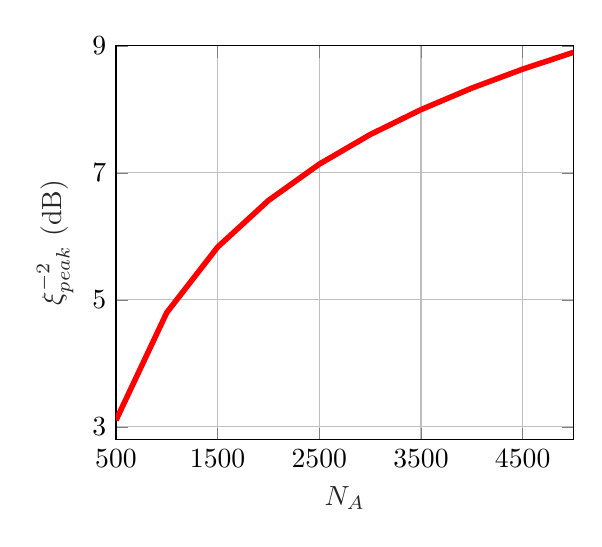
\begin{tikzpicture}

\begin{axis}[%
width=5.811cm,
height=5cm,
at={(0cm,0cm)},
scale only axis,
xmin=500.0000,
xmax=5000.0000,
xtick={500.0000,1500.0000,2500.0000,3500.0000,4500.0000},
xlabel style={font=\color{white!15!black}},
xlabel={$N_A$},
ymin=2.8000,
ymax=9.0000,
ytick={3.0000,5.0000,7.0000,9.0000},
ylabel style={font=\color{white!15!black}},
ylabel={$\xi^{-2}_{peak}$ (dB)},
axis background/.style={fill=white},
xmajorgrids,
ymajorgrids
]
\addplot [color=red, line width=2.0pt, forget plot]
  table[row sep=crcr]{%
500.0000	3.1013\\
1000.0000	4.7994\\
1500.0000	5.8299\\
2000.0000	6.5648\\
2500.0000	7.1364\\
3000.0000	7.6022\\
3500.0000	7.9950\\
4000.0000	8.3342\\
4500.0000	8.6323\\
5000.0000	8.8977\\
};
\end{axis}
\end{tikzpicture}%
      }
   \end{minipage}\vfill
   \begin{minipage}[h]{0.95\linewidth}
    %\begin{tabular}{*{2}{b{0.2\textwidth-2\tabcolsep}}}
     \subfloat[h][$\xi^{-2}_{swg}(t)$]{
       %% This file was created by matlab2tikz.
%
\begin{tikzpicture}

\begin{axis}[%
width=5.742cm,
height=5cm,
at={(0cm,0cm)},
scale only axis,
xmin=0.0000,
xmax=0.0200,
xlabel style={font=\color{white!15!black}},
xlabel={$\gamma_st$},
ymin=-0.0000,
ymax=15.0000,
ytick={0.0000,5.0000,10.0000,13.0000,15.0000},
ylabel style={font=\color{white!15!black}},
ylabel={$\xi^{-2}$ (dB)},
axis background/.style={fill=white},
xmajorgrids,
ymajorgrids
]
\addplot [color=red, line width=2.0pt, forget plot]
  table[row sep=crcr]{%
0.0000	-0.0000\\
0.0005	9.2127\\
0.0010	11.4964\\
0.0015	12.5705\\
0.0020	13.1046\\
0.0025	13.3550\\
0.0030	13.4526\\
0.0035	13.4910\\
0.0040	13.4601\\
0.0045	13.4038\\
0.0050	13.3194\\
0.0055	13.2902\\
0.0060	13.2224\\
0.0065	13.1505\\
0.0070	13.0608\\
0.0075	12.9938\\
0.0080	12.9249\\
0.0085	12.8305\\
0.0090	12.7494\\
0.0095	12.6334\\
0.0100	12.5877\\
0.0105	12.4988\\
0.0110	12.4221\\
0.0115	12.3573\\
0.0120	12.2446\\
0.0125	12.1795\\
0.0130	12.1504\\
0.0135	12.0730\\
0.0140	11.9911\\
0.0145	11.8203\\
0.0150	11.7723\\
0.0155	11.6516\\
0.0160	11.6381\\
0.0165	11.5762\\
0.0170	11.5176\\
0.0175	11.4509\\
0.0180	11.2967\\
0.0185	11.2256\\
0.0190	11.1860\\
0.0195	11.1267\\
0.0200	11.0153\\
};
\end{axis}
\end{tikzpicture}%
       \includegraphics{fig/autofig/FaradayProtocol-figure8}
       \label{fig:swg_xi_t_rp1d_NA2500}
       }
       \hfill
     \subfloat[h][$ \xi^{-2}_{peak,swg}(N_A) $]{
         \label{fig:swg_peakxi_NA_rp1d}
         \includegraphics{fig/autofig/FaradayProtocol-figure9}
         %% This file was created by matlab2tikz.
%
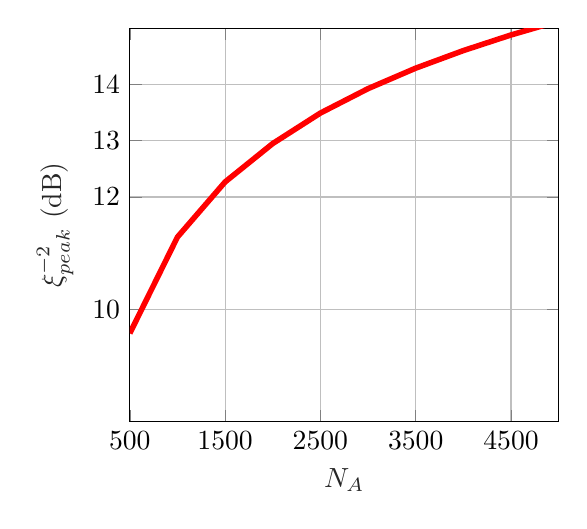
\begin{tikzpicture}

\begin{axis}[%
width=5.447cm,
height=5cm,
at={(0cm,0cm)},
scale only axis,
xmin=500.0000,
xmax=5000.0000,
xtick={500.0000,1500.0000,2500.0000,3500.0000,4500.0000},
xlabel style={font=\color{white!15!black}},
xlabel={$N_A$},
ymin=8.0000,
ymax=15.0000,
ytick={10.0000,12.0000,13.0000,14.0000,16.0000},
ylabel style={font=\color{white!15!black}},
ylabel={$\xi^{-2}_{peak}$ (dB)},
axis background/.style={fill=white},
xmajorgrids,
ymajorgrids
]
\addplot [color=red, line width=2.0pt, forget plot]
  table[row sep=crcr]{%
500.0000	9.5742\\
1000.0000	11.2863\\
1500.0000	12.2668\\
2000.0000	12.9497\\
2500.0000	13.4916\\
3000.0000	13.9257\\
3500.0000	14.2898\\
4000.0000	14.6025\\
4500.0000	14.8801\\
5000.0000	15.1264\\
};
\end{axis}
\end{tikzpicture}%
         }
   \end{minipage}
   %\end{tabular}
\caption{Spin squeezing parameter as a function of time and atom number.}\label{fig:xi_rpfix_NA_t}
\end{figure}

Apparently, the cooperativity of atom-light coupling increases as the atoms are placed closer to the waveguide surface. Figs.\ref{fig:nanofiber_peakxi_rp_NA2500} and~\ref{fig:swg_peakxi_rp_NA2500} show the inversed peak squeezing parameter as a function of $ r\!_\perp $ for both nanofiber and SWG geometries with $2500$ atoms. We find that the inversed peak squeezing parameter linearly decrease in the unit of $ dB $ or in the $ 10\log_{10} $ scale as the atoms move away from the waveguides. To explain this result, we also plot out the cooperativity, $ C_1 $, in the logarithm scale in Figs.\ref{fig:nanofiber_C1_y} and~\ref{fig:swg_C1_y} as a function of atom radial position for both waveguides. As you can see, $ \log_{10}(C_1) $ is also linearly decreasing as $ r\!_\perp $ increases. Cooperativity is indeed the key parameter to predict the peak inversed spin squeezing parameter. 


\begin{figure}[htb]
\centering
 \begin{minipage}[h]{0.95\linewidth}
 %\begin{tabular}{*{2}{b{0.2\textwidth-2\tabcolsep}}}
  \subfloat[h][$\xi^{-2}_{peak,nanofiber}(r\!_\perp)$]{
    %% This file was created by matlab2tikz.
%
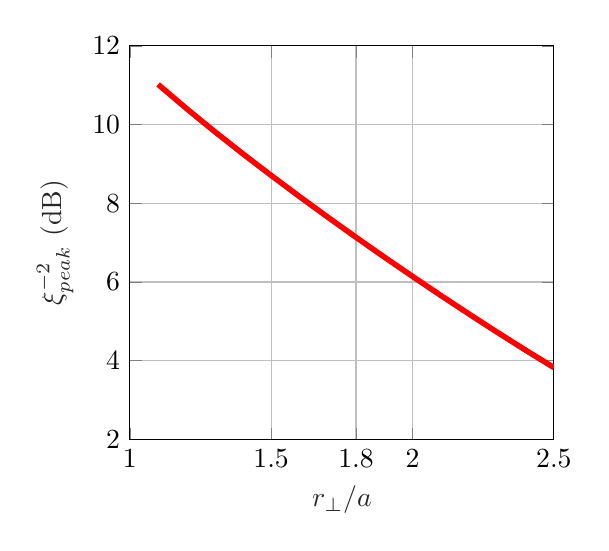
\begin{tikzpicture}

\begin{axis}[%
width=5.386cm,
height=5cm,
at={(0cm,0cm)},
scale only axis,
xmin=1.0000,
xmax=2.5000,
xtick={1.0000,1.5000,1.8000,2.0000,2.5000},
xlabel style={font=\color{white!15!black}},
xlabel={$r_\perp/a$},
ymin=2.0000,
ymax=12.0000,
ylabel style={font=\color{white!15!black}},
ylabel={$\xi^{-2}_{peak}$ (dB)},
axis background/.style={fill=white},
xmajorgrids,
ymajorgrids
]
\addplot [color=red, line width=2.0pt, forget plot]
  table[row sep=crcr]{%
1.1000	11.0198\\
1.2000	10.4084\\
1.3000	9.8223\\
1.4000	9.2556\\
1.5000	8.7068\\
1.6000	8.1716\\
1.7000	7.6484\\
1.8000	7.1364\\
1.9000	6.6338\\
2.0000	6.1423\\
2.1000	5.6591\\
2.2000	5.1855\\
2.3000	4.7217\\
2.4000	4.2688\\
2.5000	3.8276\\
};
\end{axis}
\end{tikzpicture}%
    \includegraphics{fig/autofig/FaradayProtocol-figure10}
    \label{fig:nanofiber_peakxi_rp_NA2500}
    }
    \hfill
  \subfloat[h][$ C_1(r\!_\perp) $ of a nanofiber]{
      \label{fig:nanofiber_C1_y}
      \includegraphics{fig/autofig/FaradayProtocol-figure11}
      %% This file was created by matlab2tikz.
%
%The latest updates can be retrieved from
%  http://www.mathworks.com/matlabcentral/fileexchange/22022-matlab2tikz-matlab2tikz
%where you can also make suggestions and rate matlab2tikz.
%
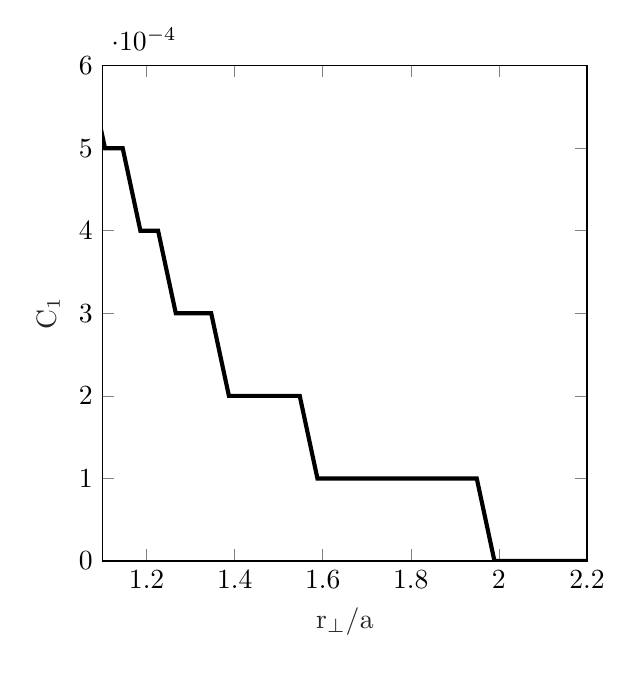
\begin{tikzpicture}

\begin{axis}[%
width=2.422in,
height=2.477in,
at={(0.406in,0.413in)},
scale only axis,
xmin=1.1000,
xmax=2.2000,
xlabel style={font=\color{white!15!black}},
xlabel={$\text{r}_\perp\text{/a}$},
ymin=0.0000,
ymax=0.0006,
ylabel style={font=\color{white!15!black}},
ylabel={$\text{C}_\text{1}$},
axis background/.style={fill=white}
]
\addplot [color=black, line width=1.5pt, forget plot]
  table[row sep=crcr]{%
1.0653	0.0006\\
1.1055	0.0005\\
1.1457	0.0005\\
1.1859	0.0004\\
1.2261	0.0004\\
1.2663	0.0003\\
1.3065	0.0003\\
1.3467	0.0003\\
1.3869	0.0002\\
1.4271	0.0002\\
1.4673	0.0002\\
1.5075	0.0002\\
1.5477	0.0002\\
1.5879	0.0001\\
1.6281	0.0001\\
1.6683	0.0001\\
1.7085	0.0001\\
1.7487	0.0001\\
1.7889	0.0001\\
1.8291	0.0001\\
1.8693	0.0001\\
1.9095	0.0001\\
1.9497	0.0001\\
1.9899	0.0000\\
2.0302	0.0000\\
2.0704	0.0000\\
2.1106	0.0000\\
2.1508	0.0000\\
2.2312	0.0000\\
};
\end{axis}
\end{tikzpicture}%
      }
   \end{minipage}\vfill
   \begin{minipage}[h]{0.95\linewidth}
    %\begin{tabular}{*{2}{b{0.2\textwidth-2\tabcolsep}}}
     \subfloat[h][$\xi^{-2}_{peak,swg}(r\!_\perp)$]{
       %% This file was created by matlab2tikz.
%
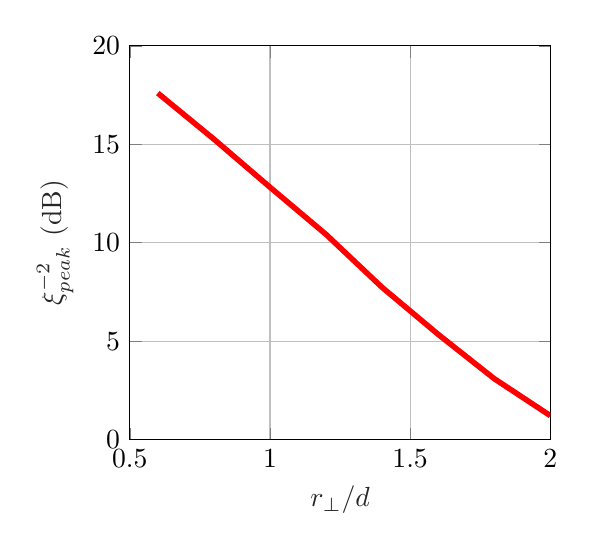
\begin{tikzpicture}

\begin{axis}[%
width=5.341cm,
height=5cm,
at={(0cm,0cm)},
scale only axis,
xmin=0.5000,
xmax=2.0000,
xtick={0.5000,1.0000,1.5000,2.0000},
xlabel style={font=\color{white!15!black}},
xlabel={$r_\perp/d$},
ymin=0.0000,
ymax=20.0000,
ylabel style={font=\color{white!15!black}},
ylabel={$\xi^{-2}_{peak}$ (dB)},
axis background/.style={fill=white},
xmajorgrids,
ymajorgrids
]
\addplot [color=red, line width=2.0pt, forget plot]
  table[row sep=crcr]{%
0.6000	17.5969\\
0.8000	15.2582\\
1.0000	12.8169\\
1.2000	10.4185\\
1.4000	7.7272\\
1.6000	5.3402\\
1.8000	3.0891\\
2.0000	1.2100\\
};
\end{axis}
\end{tikzpicture}%
       \includegraphics{fig/autofig/FaradayProtocol-figure12}
       \label{fig:swg_peakxi_rp_NA2500}
       }
       \hfill
     \subfloat[h][$ C_1(r\!_\perp) $ of a SWG]{
         \label{fig:swg_C1_y}
         \includegraphics{fig/autofig/FaradayProtocol-figure13}
         %% This file was created by matlab2tikz.
%
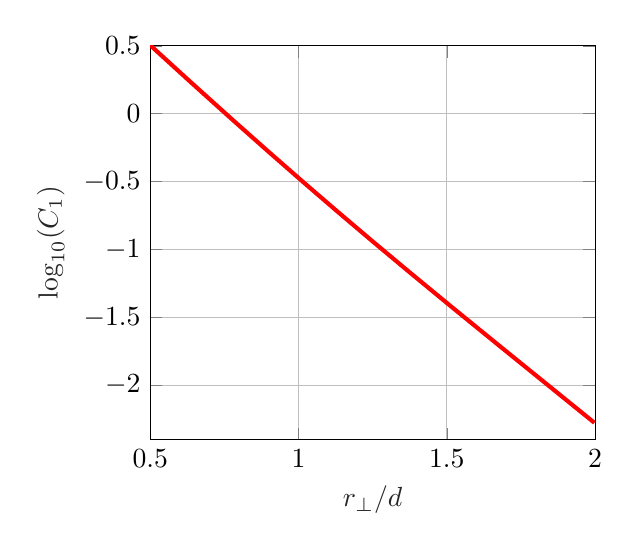
\begin{tikzpicture}

\begin{axis}[%
width=5.65cm,
height=5cm,
at={(0cm,0cm)},
scale only axis,
xmin=0.5000,
xmax=2.0000,
xlabel style={font=\color{white!15!black}},
xlabel={$r_\perp/d$},
ymin=-2.4000,
ymax=0.5000,
ylabel style={font=\color{white!15!black}},
ylabel={$\log_{10}(C_1)$},
axis background/.style={fill=white},
xmajorgrids,
ymajorgrids
]
\addplot [color=red, line width=1.5pt, forget plot]
  table[row sep=crcr]{%
0.5000	0.5041\\
0.6343	0.2366\\
0.7736	-0.0373\\
0.8980	-0.2786\\
1.0174	-0.5068\\
1.1318	-0.7220\\
1.2512	-0.9432\\
1.3756	-1.1702\\
1.5149	-1.4210\\
1.6791	-1.7132\\
1.9975	-2.2766\\
};
\end{axis}
\end{tikzpicture}%
         }
   \end{minipage}
   %\end{tabular}
\caption{Peak squeezing parameter and cooperativity as a function of atom position.}\label{fig:peakxi_rp_NA}
\end{figure}


\section{Conclusion and outlook}


\bibliography{refs/Archive}

%===============Appendix================= %
\begin{appendix}
\section{Relationships between some collective operators and the first- and second-moments in the symmetric subspace} \label{Appendix::collectivespinoperators}

Using the definitions of the atomic angular momentum operators in the $ x $-basis and the collective atomic operators, one can derive the relations between collective angular momentum operators and microscopic $\sigma_{ba}$ operators in the qutrit symmetric subspace. Below, we only present the formulas of $ \expect{\hat{F}_x} $ and $ \Delta F^2_z $ which are required to calculate the spin squeezing parameter.
\begin{subequations}
	\begin{align}
	\expect{\hat{F}_x} &= \sum_i^{N_A}\expect{\hat{f}_x}\nonumber\\
	&= -N_A \left[f\expect{\sigmauu}+(f-1)\expect{\sigmadd}+(f-2)\expect{\sigmatt } \right]\\
	\Delta F_z^2 &= N_A\expect{\Delta f_z^2} + N_A(N_A-1)\expect{\Delta f_z^{(1)}\Delta f_z^{(2)} }_s\nn\\
	&=N_A\left\{ \frac{f}{2}\left(\expect{\sigmauu}+\expect{\sigmadd}-2\expect{\sigmaud}\expect{\sigmadu}-\expect{\sigmaud}^2-\expect{\sigmadu}^2 \right)\right. \nn\\
	&\quad\quad+ \frac{2f-1}{2}\left(\expect{\sigmadd}+\expect{\sigmatt}-2\expect{\sigmadt}\expect{\sigmatd}-\expect{\sigmadt}^2-\expect{\sigmatd}^2 \right)\nn\\
	&\quad\quad +\left. \frac{\sqrt{f(2f-1)}}{2}\left[\expect{\sigmaut }+\expect{\sigmatu} -2\expect{\sigmaud}(\expect{\sigmadt}+\expect{\sigmatd}) -2\expect{\sigmadu}(\expect{\sigmadt}+\expect{\sigmatd} ) \right] \right\}\nn\\
	&\quad +N_A(N_A-1)\left[\frac{f}{2}(\expect{\Dsigmaud^{(1)}\Dsigmaud^{(2)} }_s +2\expect{\Dsigmaud^{(1)}\Dsigmadu^{(2)} }_s+\expect{\Dsigmadu^{(1)}\Dsigmadu^{(2)} }_s )\right.\\
	&\quad\quad + \frac{2f-1}{2}(\expect{\Dsigmadt^{(1)}\Dsigmadt^{(2)} }_s +2\expect{\Dsigmadt^{(1)}\Dsigmatd^{(2)} }_s +\expect{\Dsigmatd^{(1)}\Dsigmatd^{(2)} }_s) \nn\\
	&\quad\quad + \left. \sqrt{f(2f-1)}(\expect{\Dsigmaud^{(1)}\Dsigmadt^{(2)} }_s +\expect{\Dsigmaud^{(1)}\Dsigmatd^{(2)} }_s +\expect{\Dsigmadu^{(1)}\Dsigmadt^{(2)} }_s+\expect{\Dsigmadu^{(1)}\Dsigmatd^{(2)} }_s )\right]\nn
	\end{align}
\end{subequations}



\end{appendix}
\end{document}
